\documentclass{book}
\usepackage[a4paper,top=2.5cm,bottom=2.5cm,left=2.5cm,right=2.5cm]{geometry}
\usepackage{makeidx}
\usepackage{natbib}
\usepackage{graphicx}
\usepackage{multicol}
\usepackage{float}
\usepackage{listings}
\usepackage{color}
\usepackage{ifthen}
\usepackage[table]{xcolor}
\usepackage{textcomp}
\usepackage{alltt}
\usepackage[utf8]{inputenc}
\usepackage{mathptmx}
\usepackage[scaled=.90]{helvet}
\usepackage{courier}
\usepackage{sectsty}
\usepackage{amssymb}
\usepackage[titles]{tocloft}
\usepackage{doxygen}
\lstset{language=C++,inputencoding=utf8,basicstyle=\footnotesize,breaklines=true,breakatwhitespace=true,tabsize=8,numbers=left }
\makeindex
\setcounter{tocdepth}{3}
\renewcommand{\footrulewidth}{0.4pt}
\renewcommand{\familydefault}{\sfdefault}
\hfuzz=15pt
\setlength{\emergencystretch}{15pt}
\hbadness=750
\tolerance=750
\begin{document}
\begin{titlepage}
\vspace*{7cm}
\begin{center}
{\Large Basic Tensor Algebra Subprograms (B\-T\-A\-S) \\[1ex]\large Beta 3.\-0 }\\
\vspace*{1cm}
{\large Generated by Doxygen 1.8.3.1}\\
\vspace*{0.5cm}
{\small Fri Sep 6 2013 14:36:27}\\
\end{center}
\end{titlepage}
\clearemptydoublepage
\pagenumbering{roman}
\tableofcontents
\clearemptydoublepage
\pagenumbering{arabic}
\chapter{Basic Tensor Algebra Subroutines in C/\-C++ (B\-T\-A\-S)}
\label{index}This is C++11 version of B\-T\-A\-S Dependency to B\-L\-I\-T\-Z++ library has been removed.

T\-: value type N\-: rank of array Q\-: quantum number class\section{F\-E\-A\-T\-U\-R\-E\-S}\label{index_FEATURES}

\begin{DoxyEnumerate}
\item Provided generic type array classes, T\-Array$<$\-T, N$>$, S\-T\-Array$<$\-T, N$>$, and Q\-S\-T\-Array$<$T, N, Q = \doxyref{Quantum}{p.}{d8/df8/classQuantum}$>$
\end{DoxyEnumerate}


\begin{DoxyEnumerate}
\item Defined D\-Array$<$\-N$>$ as the alias to T\-Array$<$double, N$>$ (using template alias in C++11). S\-D\-Array$<$\-N$>$ and Q\-S\-D\-Array$<$\-N, Q$>$ as well
\end{DoxyEnumerate}


\begin{DoxyEnumerate}
\item Provided L\-A\-P\-A\-C\-K interfaces written in C
\end{DoxyEnumerate}


\begin{DoxyEnumerate}
\item Provided B\-L\-A\-S/\-L\-A\-P\-A\-C\-K-\/like interfaces called with D\-Array$<$\-N$>$, S\-T\-Array$<$\-N$>$, and Q\-S\-T\-Array$<$\-N, Q$>$
\end{DoxyEnumerate}


\begin{DoxyEnumerate}
\item Provided expressive contraction, permutation, and decomposition functions
\end{DoxyEnumerate}\section{C\-O\-M\-P\-I\-L\-A\-T\-I\-O\-N}\label{index_COMPILATION}

\begin{DoxyEnumerate}
\item Compiler and Library Dependencies
\end{DoxyEnumerate}

G\-N\-U G\-C\-C 4.\-7.\-0 or later Intel C/\-C++ Compiler 13.\-0 or later

B\-O\-O\-S\-T library ({\tt http\-://www.\-boost.\-org/}) C\-B\-L\-A\-S \& L\-A\-P\-A\-C\-K library or Intel M\-K\-L library


\begin{DoxyEnumerate}
\item Build libbtas.\-a

cd \$\-B\-T\-A\-S\-\_\-\-R\-O\-O\-T/lib/ make
\end{DoxyEnumerate}


\begin{DoxyEnumerate}
\item Build your code with B\-T\-A\-S library (G\-C\-C with M\-K\-L library)

g++ -\/std=c++0x -\/\-O3 -\/fopnemp -\/\-I\$\-B\-T\-A\-S\-\_\-\-R\-O\-O\-T/include \$\-B\-T\-A\-S\-\_\-\-R\-O\-O\-T/lib/libbtas.a -\/lboost\-\_\-serialization -\/lmkl\-\_\-core -\/lmkl\-\_\-intel\-\_\-lp64 -\/lmkl\-\_\-sequential
\end{DoxyEnumerate}

For coding, {\ttfamily \$\-B\-T\-A\-S\-\_\-\-R\-O\-O\-T/lib/tests.C} and {\ttfamily \$\-B\-T\-A\-S\-\_\-\-R\-O\-O\-T/dmrg/} involves helpful example to use B\-T\-A\-S

If '-\/\-D\-\_\-\-P\-R\-I\-N\-T\-\_\-\-W\-A\-R\-N\-I\-N\-G\-S' is specified, warning that S\-D\-Array\-::reserve or S\-D\-Array\-::insert is called with prohibited (quantum number) block is printed. It gives verbose output, but helps to check undesirable behavior upon reservation and insertion. 
\chapter{Namespace Index}
\section{Namespace List}
Here is a list of all namespaces with brief descriptions\-:\begin{DoxyCompactList}
\item\contentsline{section}{{\bf boost} }{\pageref{d4/da9/namespaceboost}}{}
\item\contentsline{section}{{\bf boost\-::serialization} }{\pageref{de/d49/namespaceboost_1_1serialization}}{}
\item\contentsline{section}{{\bf btas} }{\pageref{df/daf/namespacebtas}}{}
\item\contentsline{section}{{\bf mps} }{\pageref{d1/d7b/namespacemps}}{}
\end{DoxyCompactList}

\chapter{Hierarchical Index}
\section{Class Hierarchy}
This inheritance list is sorted roughly, but not completely, alphabetically\-:\begin{DoxyCompactList}
\item \contentsline{section}{F\-C\-\_\-\-C\-O\-M\-P\-L\-E\-X\-\_\-08}{\pageref{d4/d56/structFC__COMPLEX__08}}{}
\item \contentsline{section}{F\-C\-\_\-\-C\-O\-M\-P\-L\-E\-X\-\_\-16}{\pageref{d5/d95/structFC__COMPLEX__16}}{}
\item \contentsline{section}{btas\-:\-:indexed\-\_\-loop$<$ N $>$}{\pageref{d4/d84/classbtas_1_1indexed__loop}}{}
\item \contentsline{section}{btas\-:\-:indexed\-\_\-loop$<$ 1 $>$}{\pageref{d7/d39/classbtas_1_1indexed__loop_3_011_01_4}}{}
\item \contentsline{section}{btas\-:\-:null\-\_\-deleter}{\pageref{d8/d8a/structbtas_1_1null__deleter}}{}
\item \contentsline{section}{btas\-:\-:Q\-S\-Tmerge\-Info$<$ N, Q $>$}{\pageref{d0/de7/classbtas_1_1QSTmergeInfo}}{}
\item \contentsline{section}{Quantum}{\pageref{d8/df8/classQuantum}}{}
\item \contentsline{section}{btas\-:\-:S\-T\-Array$<$ T, N $>$}{\pageref{d7/d05/classbtas_1_1STArray}}{}
\begin{DoxyCompactList}
\item \contentsline{section}{btas\-:\-:Q\-S\-T\-Array$<$ T, N, Q $>$}{\pageref{db/dff/classbtas_1_1QSTArray}}{}
\end{DoxyCompactList}
\item \contentsline{section}{btas\-:\-:T\-\_\-arglist\-\_\-base}{\pageref{d7/dd4/classbtas_1_1T__arglist__base}}{}
\begin{DoxyCompactList}
\item \contentsline{section}{btas\-:\-:C\-\_\-arglist\-\_\-triple$<$ T, N1, N2, N3 $>$}{\pageref{d5/d67/classbtas_1_1C__arglist__triple}}{}
\item \contentsline{section}{btas\-:\-:R\-\_\-arglist\-\_\-double$<$ T, N1, N2 $>$}{\pageref{d5/dcd/classbtas_1_1R__arglist__double}}{}
\item \contentsline{section}{btas\-:\-:R\-\_\-arglist\-\_\-quadra$<$ T, N1, N2, N3, N4 $>$}{\pageref{d4/dec/classbtas_1_1R__arglist__quadra}}{}
\item \contentsline{section}{btas\-:\-:R\-\_\-arglist\-\_\-single$<$ T, N1 $>$}{\pageref{d5/d3b/classbtas_1_1R__arglist__single}}{}
\item \contentsline{section}{btas\-:\-:R\-\_\-arglist\-\_\-triple$<$ T, N1, N2, N3 $>$}{\pageref{dd/d0a/classbtas_1_1R__arglist__triple}}{}
\item \contentsline{section}{btas\-:\-:C\-\_\-arglist\-\_\-triple$<$ double, N\-A, N\-B, N\-C $>$}{\pageref{d5/d67/classbtas_1_1C__arglist__triple}}{}
\begin{DoxyCompactList}
\item \contentsline{section}{btas\-:\-:Dgemm\-Arglist$<$ N\-A, N\-B, N\-C $>$}{\pageref{d6/d9b/classbtas_1_1DgemmArglist}}{}
\item \contentsline{section}{btas\-:\-:Dgemv\-Arglist$<$ N\-A, N\-B, N\-C $>$}{\pageref{df/d7c/classbtas_1_1DgemvArglist}}{}
\item \contentsline{section}{btas\-:\-:Dger\-Arglist$<$ N\-A, N\-B, N\-C $>$}{\pageref{da/db6/classbtas_1_1DgerArglist}}{}
\end{DoxyCompactList}
\item \contentsline{section}{btas\-:\-:R\-\_\-arglist\-\_\-double$<$ double, N, N $>$}{\pageref{d5/dcd/classbtas_1_1R__arglist__double}}{}
\begin{DoxyCompactList}
\item \contentsline{section}{btas\-:\-:Daxpy\-Arglist$<$ N $>$}{\pageref{d3/d12/classbtas_1_1DaxpyArglist}}{}
\item \contentsline{section}{btas\-:\-:Dcopy\-Arglist$<$ N $>$}{\pageref{d9/dfc/classbtas_1_1DcopyArglist}}{}
\item \contentsline{section}{btas\-:\-:Dpermute\-Arglist$<$ N $>$}{\pageref{d6/d58/classbtas_1_1DpermuteArglist}}{}
\end{DoxyCompactList}
\item \contentsline{section}{btas\-:\-:R\-\_\-arglist\-\_\-quadra$<$ double, N\-A, 1, N\-U, N\-A-\/\-N\-U+2 $>$}{\pageref{d4/dec/classbtas_1_1R__arglist__quadra}}{}
\begin{DoxyCompactList}
\item \contentsline{section}{btas\-:\-:Dgesvd\-Arglist$<$ N\-A, N\-U $>$}{\pageref{d5/d3c/classbtas_1_1DgesvdArglist}}{}
\end{DoxyCompactList}
\item \contentsline{section}{btas\-:\-:R\-\_\-arglist\-\_\-single$<$ double, N $>$}{\pageref{d5/d3b/classbtas_1_1R__arglist__single}}{}
\begin{DoxyCompactList}
\item \contentsline{section}{btas\-:\-:Dscal\-Arglist$<$ N $>$}{\pageref{d0/d2f/classbtas_1_1DscalArglist}}{}
\end{DoxyCompactList}
\end{DoxyCompactList}
\item \contentsline{section}{btas\-:\-:T\-Array$<$ T, N $>$}{\pageref{db/d3c/classbtas_1_1TArray}}{}
\begin{DoxyCompactList}
\item \contentsline{section}{btas\-:\-:T\-Sub\-Array$<$ T, N $>$}{\pageref{da/d50/classbtas_1_1TSubArray}}{}
\end{DoxyCompactList}
\item \contentsline{section}{time\-\_\-stamp}{\pageref{d2/d9d/classtime__stamp}}{}
\item vector\begin{DoxyCompactList}
\item \contentsline{section}{btas\-:\-:Qshapes$<$ Q $>$}{\pageref{dd/df1/classbtas_1_1Qshapes}}{}
\end{DoxyCompactList}
\end{DoxyCompactList}

\chapter{Data Structure Index}
\section{Data Structures}
Here are the data structures with brief descriptions\-:\begin{DoxyCompactList}
\item\contentsline{section}{{\bf btas\-::\-C\-\_\-arglist\-\_\-triple$<$ T, N1, N2, N3 $>$} \\*Argment list for contraction }{\pageref{d5/d67/classbtas_1_1C__arglist__triple}}{}
\item\contentsline{section}{{\bf btas\-::\-Daxpy\-Arglist$<$ N $>$} }{\pageref{d3/d12/classbtas_1_1DaxpyArglist}}{}
\item\contentsline{section}{{\bf btas\-::\-Dcopy\-Arglist$<$ N $>$} }{\pageref{d9/dfc/classbtas_1_1DcopyArglist}}{}
\item\contentsline{section}{{\bf btas\-::\-Dgemm\-Arglist$<$ N\-A, N\-B, N\-C $>$} }{\pageref{d6/d9b/classbtas_1_1DgemmArglist}}{}
\item\contentsline{section}{{\bf btas\-::\-Dgemv\-Arglist$<$ N\-A, N\-B, N\-C $>$} }{\pageref{df/d7c/classbtas_1_1DgemvArglist}}{}
\item\contentsline{section}{{\bf btas\-::\-Dger\-Arglist$<$ N\-A, N\-B, N\-C $>$} }{\pageref{da/db6/classbtas_1_1DgerArglist}}{}
\item\contentsline{section}{{\bf btas\-::\-Dgesvd\-Arglist$<$ N\-A, N\-U $>$} }{\pageref{d5/d3c/classbtas_1_1DgesvdArglist}}{}
\item\contentsline{section}{{\bf btas\-::\-Dpermute\-Arglist$<$ N $>$} }{\pageref{d6/d58/classbtas_1_1DpermuteArglist}}{}
\item\contentsline{section}{{\bf btas\-::\-Dscal\-Arglist$<$ N $>$} }{\pageref{d0/d2f/classbtas_1_1DscalArglist}}{}
\item\contentsline{section}{{\bf F\-C\-\_\-\-C\-O\-M\-P\-L\-E\-X\-\_\-08} }{\pageref{d4/d56/structFC__COMPLEX__08}}{}
\item\contentsline{section}{{\bf F\-C\-\_\-\-C\-O\-M\-P\-L\-E\-X\-\_\-16} }{\pageref{d5/d95/structFC__COMPLEX__16}}{}
\item\contentsline{section}{{\bf btas\-::indexed\-\_\-loop$<$ N $>$} \\*Indexed loop for array object }{\pageref{d4/d84/classbtas_1_1indexed__loop}}{}
\item\contentsline{section}{{\bf btas\-::indexed\-\_\-loop$<$ 1 $>$} }{\pageref{d7/d39/classbtas_1_1indexed__loop_3_011_01_4}}{}
\item\contentsline{section}{{\bf btas\-::null\-\_\-deleter} \\*Null-\/deleter }{\pageref{d8/d8a/structbtas_1_1null__deleter}}{}
\item\contentsline{section}{{\bf btas\-::\-Qshapes$<$ Q $>$} \\*\doxyref{Quantum}{p.}{d8/df8/classQuantum} number vector }{\pageref{dd/df1/classbtas_1_1Qshapes}}{}
\item\contentsline{section}{{\bf btas\-::\-Q\-S\-T\-Array$<$ T, N, Q $>$} \\*\doxyref{Quantum}{p.}{d8/df8/classQuantum} number-\/based block sparse array }{\pageref{db/dff/classbtas_1_1QSTArray}}{}
\item\contentsline{section}{{\bf btas\-::\-Q\-S\-Tmerge\-Info$<$ N, Q $>$} \\*Merged index infomation by quantum number-\/based sparse array }{\pageref{d0/de7/classbtas_1_1QSTmergeInfo}}{}
\item\contentsline{section}{{\bf Quantum} \\*Default quantum number class }{\pageref{d8/df8/classQuantum}}{}
\item\contentsline{section}{{\bf btas\-::\-R\-\_\-arglist\-\_\-double$<$ T, N1, N2 $>$} \\*Replication argment list for double argments function }{\pageref{d5/dcd/classbtas_1_1R__arglist__double}}{}
\item\contentsline{section}{{\bf btas\-::\-R\-\_\-arglist\-\_\-quadra$<$ T, N1, N2, N3, N4 $>$} \\*Replication argment list for quadruple argments function }{\pageref{d4/dec/classbtas_1_1R__arglist__quadra}}{}
\item\contentsline{section}{{\bf btas\-::\-R\-\_\-arglist\-\_\-single$<$ T, N1 $>$} \\*Replication argment list for single argment function }{\pageref{d5/d3b/classbtas_1_1R__arglist__single}}{}
\item\contentsline{section}{{\bf btas\-::\-R\-\_\-arglist\-\_\-triple$<$ T, N1, N2, N3 $>$} \\*Replication argment list for triple argments function }{\pageref{dd/d0a/classbtas_1_1R__arglist__triple}}{}
\item\contentsline{section}{{\bf btas\-::\-S\-T\-Array$<$ T, N $>$} \\*Block-\/sparse array class }{\pageref{d7/d05/classbtas_1_1STArray}}{}
\item\contentsline{section}{{\bf btas\-::\-T\-\_\-arglist\-\_\-base} \\*Base class of argment list }{\pageref{d7/dd4/classbtas_1_1T__arglist__base}}{}
\item\contentsline{section}{{\bf btas\-::\-T\-Array$<$ T, N $>$} \\*Dense array class }{\pageref{db/d3c/classbtas_1_1TArray}}{}
\item\contentsline{section}{{\bf time\-\_\-stamp} \\*Clock function for timing }{\pageref{d2/d9d/classtime__stamp}}{}
\item\contentsline{section}{{\bf btas\-::\-T\-Sub\-Array$<$ T, N $>$} \\*Sub-\/array of dense array \doxyref{T\-Array}{p.}{db/d3c/classbtas_1_1TArray} }{\pageref{da/d50/classbtas_1_1TSubArray}}{}
\end{DoxyCompactList}

\chapter{File Index}
\section{File List}
Here is a list of all files with brief descriptions\-:\begin{DoxyCompactList}
\item\contentsline{section}{include/{\bf contract.\-h} }{\pageref{dd/d9c/contract_8h}}{}
\item\contentsline{section}{include/{\bf decompose.\-h} \\*B\-T\-A\-S driver routines for tensor decomposition }{\pageref{df/dfc/decompose_8h}}{}
\item\contentsline{section}{include/{\bf indexed\-\_\-loop.\-h} }{\pageref{d0/d6e/indexed__loop_8h}}{}
\item\contentsline{section}{include/{\bf permute.\-h} }{\pageref{df/da6/permute_8h}}{}
\item\contentsline{section}{include/{\bf time\-\_\-stamp.\-h} }{\pageref{d3/dd0/time__stamp_8h}}{}
\item\contentsline{section}{include/btas/{\bf blas\-\_\-cxx\-\_\-interface.\-h} }{\pageref{dd/d03/blas__cxx__interface_8h}}{}
\item\contentsline{section}{include/btas/{\bf btas.\-h} }{\pageref{d9/d0b/btas_8h}}{}
\item\contentsline{section}{include/btas/{\bf btas\-\_\-contract\-\_\-shape.\-h} }{\pageref{dd/d9e/btas__contract__shape_8h}}{}
\item\contentsline{section}{include/btas/{\bf btas\-\_\-permute\-\_\-shape.\-h} }{\pageref{dc/d2e/btas__permute__shape_8h}}{}
\item\contentsline{section}{include/btas/{\bf Targlist.\-h} }{\pageref{d6/d01/Targlist_8h}}{}
\item\contentsline{section}{include/btas/{\bf T\-Vector.\-h} \\*Utility functions for fixed and variable size vectors }{\pageref{da/dd8/TVector_8h}}{}
\item\contentsline{section}{include/btas/\-D\-E\-N\-S\-E/{\bf C\-Array.\-h} \\*Dense array for single precision complex number }{\pageref{d9/d78/CArray_8h}}{}
\item\contentsline{section}{include/btas/\-D\-E\-N\-S\-E/{\bf Darglist.\-h} }{\pageref{d4/d22/Darglist_8h}}{}
\item\contentsline{section}{include/btas/\-D\-E\-N\-S\-E/{\bf D\-Array.\-h} \\*Dense array for double precision real number }{\pageref{d3/d5c/DArray_8h}}{}
\item\contentsline{section}{include/btas/\-D\-E\-N\-S\-E/{\bf Dblas.\-h} \\*B\-L\-A\-S wrappers for double precision real array }{\pageref{de/d3a/Dblas_8h}}{}
\item\contentsline{section}{include/btas/\-D\-E\-N\-S\-E/{\bf Dcontract.\-h} }{\pageref{db/da1/Dcontract_8h}}{}
\item\contentsline{section}{include/btas/\-D\-E\-N\-S\-E/{\bf Ddiagonal.\-h} }{\pageref{df/db2/Ddiagonal_8h}}{}
\item\contentsline{section}{include/btas/\-D\-E\-N\-S\-E/{\bf Dlapack.\-h} \\*L\-A\-P\-A\-C\-K wrappers for double precision real array }{\pageref{d3/da7/Dlapack_8h}}{}
\item\contentsline{section}{include/btas/\-D\-E\-N\-S\-E/{\bf Dpermute.\-h} }{\pageref{d2/d18/Dpermute_8h}}{}
\item\contentsline{section}{include/btas/\-D\-E\-N\-S\-E/{\bf Dreindex.\-h} }{\pageref{d4/d02/Dreindex_8h}}{}
\item\contentsline{section}{include/btas/\-D\-E\-N\-S\-E/{\bf S\-Array.\-h} \\*Dense array for single precision real number }{\pageref{de/d0d/SArray_8h}}{}
\item\contentsline{section}{include/btas/\-D\-E\-N\-S\-E/{\bf T\-Array.\-h} }{\pageref{df/d8f/TArray_8h}}{}
\item\contentsline{section}{include/btas/\-D\-E\-N\-S\-E/{\bf T\-Sub\-Array.\-h} \\*Dense sub-\/array class and its copy semantics }{\pageref{d8/d46/TSubArray_8h}}{}
\item\contentsline{section}{include/btas/\-D\-E\-N\-S\-E/{\bf Z\-Array.\-h} \\*Dense array for double precision complex number }{\pageref{d4/dc1/ZArray_8h}}{}
\item\contentsline{section}{include/btas/\-M\-P\-S/{\bf M\-P\-Sblas.\-h} }{\pageref{de/d28/MPSblas_8h}}{}
\item\contentsline{section}{include/btas/\-Q\-S\-P\-A\-R\-S\-E/{\bf btas\-\_\-contract\-\_\-qshape.\-h} \\*\doxyref{Quantum}{p.}{d8/df8/classQuantum} number contraction for quantum number-\/based sparse B\-L\-A\-S calls }{\pageref{df/db6/btas__contract__qshape_8h}}{}
\item\contentsline{section}{include/btas/\-Q\-S\-P\-A\-R\-S\-E/{\bf Q\-S\-D\-Array.\-h} }{\pageref{d9/dd2/QSDArray_8h}}{}
\item\contentsline{section}{include/btas/\-Q\-S\-P\-A\-R\-S\-E/{\bf Q\-S\-Dblas.\-h} \\*B\-L\-A\-S wrappers for quantum number-\/based sparse array contractions }{\pageref{d3/d2f/QSDblas_8h}}{}
\item\contentsline{section}{include/btas/\-Q\-S\-P\-A\-R\-S\-E/{\bf Q\-S\-Dcontract.\-h} \\*Convenient contraction functions for Q\-S\-D\-Array }{\pageref{dc/d13/QSDcontract_8h}}{}
\item\contentsline{section}{include/btas/\-Q\-S\-P\-A\-R\-S\-E/{\bf Q\-S\-Dlapack.\-h} }{\pageref{de/d28/QSDlapack_8h}}{}
\item\contentsline{section}{include/btas/\-Q\-S\-P\-A\-R\-S\-E/{\bf Q\-S\-Dmerge.\-h} \\*Aliases of Q\-S\-Tmerge and Q\-S\-Texpand for double precision real array }{\pageref{d3/dcb/QSDmerge_8h}}{}
\item\contentsline{section}{include/btas/\-Q\-S\-P\-A\-R\-S\-E/{\bf Q\-S\-Dpermute.\-h} \\*Array permutation for Q\-S\-D\-Array }{\pageref{d5/dc2/QSDpermute_8h}}{}
\item\contentsline{section}{include/btas/\-Q\-S\-P\-A\-R\-S\-E/{\bf Qshapes.\-h} }{\pageref{d1/d66/Qshapes_8h}}{}
\item\contentsline{section}{include/btas/\-Q\-S\-P\-A\-R\-S\-E/{\bf Q\-S\-T\-Array.\-h} }{\pageref{de/df8/QSTArray_8h}}{}
\item\contentsline{section}{include/btas/\-Q\-S\-P\-A\-R\-S\-E/{\bf Q\-S\-Tdsum.\-h} }{\pageref{d2/d1f/QSTdsum_8h}}{}
\item\contentsline{section}{include/btas/\-Q\-S\-P\-A\-R\-S\-E/{\bf Q\-S\-Tmerge.\-h} \\*Merging and expanding array indices }{\pageref{dd/df2/QSTmerge_8h}}{}
\item\contentsline{section}{include/btas/\-Q\-S\-P\-A\-R\-S\-E/{\bf Q\-S\-Tmerge\-Info.\-h} }{\pageref{d5/d49/QSTmergeInfo_8h}}{}
\item\contentsline{section}{include/btas/\-Q\-S\-P\-A\-R\-S\-E/{\bf Quantum.\-h} \\*Default quantum number class named \doxyref{Quantum}{p.}{d8/df8/classQuantum} }{\pageref{d0/d45/Quantum_8h}}{}
\item\contentsline{section}{include/btas/\-S\-P\-A\-R\-S\-E/{\bf btas\-\_\-contract\-\_\-dshape.\-h} \\*Block-\/shape contraction for sparse array B\-L\-A\-S calls }{\pageref{de/d95/btas__contract__dshape_8h}}{}
\item\contentsline{section}{include/btas/\-S\-P\-A\-R\-S\-E/{\bf S\-D\-Array.\-h} }{\pageref{da/da3/SDArray_8h}}{}
\item\contentsline{section}{include/btas/\-S\-P\-A\-R\-S\-E/{\bf S\-Dblas.\-h} }{\pageref{d6/de7/SDblas_8h}}{}
\item\contentsline{section}{include/btas/\-S\-P\-A\-R\-S\-E/{\bf S\-Dcontract.\-h} }{\pageref{db/d3c/SDcontract_8h}}{}
\item\contentsline{section}{include/btas/\-S\-P\-A\-R\-S\-E/{\bf S\-Ddiagonal.\-h} }{\pageref{d8/d3e/SDdiagonal_8h}}{}
\item\contentsline{section}{include/btas/\-S\-P\-A\-R\-S\-E/{\bf S\-Dpermute.\-h} }{\pageref{d5/d38/SDpermute_8h}}{}
\item\contentsline{section}{include/btas/\-S\-P\-A\-R\-S\-E/{\bf S\-T\-Array.\-h} }{\pageref{d8/d9f/STArray_8h}}{}
\item\contentsline{section}{include/btas/\-S\-P\-A\-R\-S\-E/{\bf S\-Tdsum.\-h} }{\pageref{d9/dc3/STdsum_8h}}{}
\item\contentsline{section}{include/lapack/{\bf clapack.\-h} \\*C/\-C++ interface to lapack calls like clapack\-\_\-xxx }{\pageref{d6/d79/clapack_8h}}{}
\item\contentsline{section}{include/lapack/{\bf lapack\-\_\-fort\-\_\-predecl.\-h} }{\pageref{d9/dcd/lapack__fort__predecl_8h}}{}
\item\contentsline{section}{lib/{\bf clapack.\-C} }{\pageref{d2/de8/clapack_8C}}{}
\item\contentsline{section}{lib/{\bf Dreindex.\-C} }{\pageref{d0/d4a/Dreindex_8C}}{}
\item\contentsline{section}{lib/{\bf libbtas.\-C} }{\pageref{d4/d96/libbtas_8C}}{}
\item\contentsline{section}{lib/{\bf tests.\-C} }{\pageref{d6/dd2/tests_8C}}{}
\end{DoxyCompactList}

\chapter{Namespace Documentation}
\section{boost Namespace Reference}
\label{d4/da9/namespaceboost}\index{boost@{boost}}
\subsection*{Namespaces}
\begin{DoxyCompactItemize}
\item 
namespace {\bf serialization}
\end{DoxyCompactItemize}

\section{boost\-:\-:serialization Namespace Reference}
\label{de/d49/namespaceboost_1_1serialization}\index{boost\-::serialization@{boost\-::serialization}}
\subsection*{Functions}
\begin{DoxyCompactItemize}
\item 
{\footnotesize template$<$class Archive , typename T , size\-\_\-t N$>$ }\\void {\bf serialize} (Archive \&ar, std\-::array$<$ T, N $>$ \&vec, const unsigned int version)
\begin{DoxyCompactList}\small\item\em Enables to use boost serialization. \end{DoxyCompactList}\end{DoxyCompactItemize}


\subsection{Function Documentation}
\index{boost\-::serialization@{boost\-::serialization}!serialize@{serialize}}
\index{serialize@{serialize}!boost::serialization@{boost\-::serialization}}
\subsubsection[{serialize}]{\setlength{\rightskip}{0pt plus 5cm}template$<$class Archive , typename T , size\-\_\-t N$>$ void boost\-::serialization\-::serialize (
\begin{DoxyParamCaption}
\item[{Archive \&}]{ar, }
\item[{std\-::array$<$ T, N $>$ \&}]{vec, }
\item[{const unsigned int}]{version}
\end{DoxyParamCaption}
)}\label{de/d49/namespaceboost_1_1serialization_ae00994c01069657b87786f512bf43809}


Enables to use boost serialization. 



Definition at line 34 of file T\-Vector.\-h.


\section{btas Namespace Reference}
\label{df/daf/namespacebtas}\index{btas@{btas}}
\subsection*{Data Structures}
\begin{DoxyCompactItemize}
\item 
struct {\bf null\-\_\-deleter}
\begin{DoxyCompactList}\small\item\em Null-\/deleter. \end{DoxyCompactList}\item 
class {\bf Dcopy\-Arglist}
\item 
class {\bf Dscal\-Arglist}
\item 
class {\bf Daxpy\-Arglist}
\item 
class {\bf Dpermute\-Arglist}
\item 
class {\bf Dgemv\-Arglist}
\item 
class {\bf Dger\-Arglist}
\item 
class {\bf Dgemm\-Arglist}
\item 
class {\bf Dgesvd\-Arglist}
\item 
class {\bf T\-Array}
\begin{DoxyCompactList}\small\item\em Dense array class. \end{DoxyCompactList}\item 
class {\bf T\-Sub\-Array}
\begin{DoxyCompactList}\small\item\em Sub-\/array of dense array \doxyref{T\-Array}{p.}{db/d3c/classbtas_1_1TArray}. \end{DoxyCompactList}\item 
class {\bf Qshapes}
\begin{DoxyCompactList}\small\item\em \doxyref{Quantum}{p.}{d8/df8/classQuantum} number vector. \end{DoxyCompactList}\item 
class {\bf Q\-S\-T\-Array}
\begin{DoxyCompactList}\small\item\em \doxyref{Quantum}{p.}{d8/df8/classQuantum} number-\/based block sparse array. \end{DoxyCompactList}\item 
class {\bf Q\-S\-Tmerge\-Info}
\begin{DoxyCompactList}\small\item\em Merged index infomation by quantum number-\/based sparse array. \end{DoxyCompactList}\item 
class {\bf S\-T\-Array}
\begin{DoxyCompactList}\small\item\em Block-\/sparse array class. \end{DoxyCompactList}\item 
class {\bf T\-\_\-arglist\-\_\-base}
\begin{DoxyCompactList}\small\item\em Base class of argment list. \end{DoxyCompactList}\item 
class {\bf R\-\_\-arglist\-\_\-single}
\begin{DoxyCompactList}\small\item\em Replication argment list for single argment function. \end{DoxyCompactList}\item 
class {\bf R\-\_\-arglist\-\_\-double}
\begin{DoxyCompactList}\small\item\em Replication argment list for double argments function. \end{DoxyCompactList}\item 
class {\bf R\-\_\-arglist\-\_\-triple}
\begin{DoxyCompactList}\small\item\em Replication argment list for triple argments function. \end{DoxyCompactList}\item 
class {\bf R\-\_\-arglist\-\_\-quadra}
\begin{DoxyCompactList}\small\item\em Replication argment list for quadruple argments function. \end{DoxyCompactList}\item 
class {\bf C\-\_\-arglist\-\_\-triple}
\begin{DoxyCompactList}\small\item\em Argment list for contraction. \end{DoxyCompactList}\item 
class {\bf indexed\-\_\-loop}
\begin{DoxyCompactList}\small\item\em Indexed loop for array object. \end{DoxyCompactList}\item 
class {\bf indexed\-\_\-loop$<$ 1 $>$}
\end{DoxyCompactItemize}
\subsection*{Typedefs}
\begin{DoxyCompactItemize}
\item 
typedef unsigned int {\bf uint}
\item 
typedef unsigned long {\bf wint}
\item 
typedef std\-::vector$<$ int $>$ {\bf Dshapes}
\begin{DoxyCompactList}\small\item\em Alias to dense shape. \end{DoxyCompactList}\item 
{\footnotesize template$<$size\-\_\-t N$>$ }\\using {\bf C\-Array} = {\bf T\-Array}$<$ complex$<$ float $>$, N $>$
\begin{DoxyCompactList}\small\item\em Alias to single precision complex array. \end{DoxyCompactList}\item 
{\footnotesize template$<$size\-\_\-t N$>$ }\\using {\bf C\-Sub\-Array} = {\bf T\-Sub\-Array}$<$ complex$<$ float $>$, N $>$
\begin{DoxyCompactList}\small\item\em Alias to single precision complex sub-\/array. \end{DoxyCompactList}\item 
{\footnotesize template$<$size\-\_\-t N$>$ }\\using {\bf D\-Array} = {\bf T\-Array}$<$ double, N $>$
\begin{DoxyCompactList}\small\item\em Alias to double precision real array. \end{DoxyCompactList}\item 
{\footnotesize template$<$size\-\_\-t N$>$ }\\using {\bf D\-Sub\-Array} = {\bf T\-Sub\-Array}$<$ double, N $>$
\begin{DoxyCompactList}\small\item\em Alias to double precision real sub-\/array. \end{DoxyCompactList}\item 
{\footnotesize template$<$size\-\_\-t N$>$ }\\using {\bf S\-Array} = {\bf T\-Array}$<$ float, N $>$
\begin{DoxyCompactList}\small\item\em Alias to single precision real array. \end{DoxyCompactList}\item 
{\footnotesize template$<$size\-\_\-t N$>$ }\\using {\bf S\-Sub\-Array} = {\bf T\-Sub\-Array}$<$ float, N $>$
\begin{DoxyCompactList}\small\item\em Alias to single precision real sub-\/array. \end{DoxyCompactList}\item 
{\footnotesize template$<$size\-\_\-t N$>$ }\\using {\bf Z\-Array} = {\bf T\-Array}$<$ complex$<$ double $>$, N $>$
\begin{DoxyCompactList}\small\item\em Alias to double precision complex array. \end{DoxyCompactList}\item 
{\footnotesize template$<$size\-\_\-t N$>$ }\\using {\bf Z\-Sub\-Array} = {\bf T\-Sub\-Array}$<$ complex$<$ double $>$, N $>$
\begin{DoxyCompactList}\small\item\em Alias to double precision complex sub-\/array. \end{DoxyCompactList}\item 
{\footnotesize template$<$size\-\_\-t N, class Q  = Quantum$>$ }\\using {\bf Q\-S\-D\-Array} = {\bf Q\-S\-T\-Array}$<$ double, N, Q $>$
\begin{DoxyCompactList}\small\item\em Alias to double precision real quatum number-\/based sparse-\/array. \end{DoxyCompactList}\item 
{\footnotesize template$<$size\-\_\-t N$>$ }\\using {\bf S\-D\-Array} = {\bf S\-T\-Array}$<$ double, N $>$
\begin{DoxyCompactList}\small\item\em alias to double precision real sparse-\/array \end{DoxyCompactList}\item 
{\footnotesize template$<$typename T , size\-\_\-t N$>$ }\\using {\bf T\-Vector} = std\-::array$<$ T, N $>$
\begin{DoxyCompactList}\small\item\em Template aliases to std\-::array$<$\-T, N$>$, for convenience. \end{DoxyCompactList}\item 
{\footnotesize template$<$size\-\_\-t N$>$ }\\using {\bf I\-Vector} = std\-::array$<$ int, N $>$
\begin{DoxyCompactList}\small\item\em Template aliases to std\-::array$<$int, N$>$, for convenience. \end{DoxyCompactList}\end{DoxyCompactItemize}
\subsection*{Enumerations}
\begin{DoxyCompactItemize}
\item 
enum {\bf B\-T\-A\-S\-\_\-\-O\-R\-D\-E\-R} \{ {\bf Row\-Major} =101, 
{\bf Col\-Major} =102
 \}
\item 
enum {\bf B\-T\-A\-S\-\_\-\-T\-R\-A\-N\-S\-P\-O\-S\-E} \{ {\bf No\-Trans} =111, 
{\bf Trans} =112, 
{\bf Conj\-Trans} =113
 \}
\item 
enum {\bf B\-T\-A\-S\-\_\-\-U\-P\-L\-O} \{ {\bf Upper} =121, 
{\bf Lower} =122
 \}
\item 
enum {\bf B\-T\-A\-S\-\_\-\-D\-I\-A\-G} \{ {\bf Non\-Unit} =131, 
{\bf Unit} =132
 \}
\item 
enum {\bf B\-T\-A\-S\-\_\-\-S\-I\-D\-E} \{ {\bf Left} =141, 
{\bf Right} =142
 \}
\item 
enum {\bf B\-T\-A\-S\-\_\-\-C\-O\-N\-T\-R\-A\-C\-T\-\_\-\-T\-U\-N\-I\-N\-G} \{ \\*
{\bf J\-O\-B\-M\-A\-S\-K\-\_\-\-A\-\_\-\-P\-M\-U\-T\-E} = 0x20, 
{\bf J\-O\-B\-M\-A\-S\-K\-\_\-\-A\-\_\-\-T\-R\-A\-N\-S} = 0x10, 
{\bf J\-O\-B\-M\-A\-S\-K\-\_\-\-B\-\_\-\-P\-M\-U\-T\-E} = 0x08, 
{\bf J\-O\-B\-M\-A\-S\-K\-\_\-\-B\-\_\-\-T\-R\-A\-N\-S} = 0x04, 
\\*
{\bf J\-O\-B\-M\-A\-S\-K\-\_\-\-B\-L\-A\-S\-\_\-\-T\-Y\-P\-E} = 0x03
 \}
\item 
enum {\bf B\-T\-A\-S\-\_\-\-A\-R\-R\-O\-W\-\_\-\-D\-I\-R\-E\-C\-T\-I\-O\-N} \{ {\bf Left\-Arrow}, 
{\bf Right\-Arrow}
 \}
\begin{DoxyCompactList}\small\item\em Arrow direction of decomposed array Because S\-V\-D splits A = U $\ast$ S $\ast$ V$^\wedge$\-T, either U or V has a total quantum number equals to that of A. \end{DoxyCompactList}\end{DoxyCompactItemize}
\subsection*{Functions}
\begin{DoxyCompactItemize}
\item 
{\footnotesize template$<$size\-\_\-t N\-A, size\-\_\-t N\-B, size\-\_\-t N\-C$>$ }\\void {\bf gemv\-\_\-contract\-\_\-shape} (const {\bf B\-T\-A\-S\-\_\-\-T\-R\-A\-N\-S\-P\-O\-S\-E} \&Trans\-A, const {\bf I\-Vector}$<$ N\-A $>$ \&a\-\_\-shape, const {\bf I\-Vector}$<$ N\-B $>$ \&b\-\_\-shape, {\bf I\-Vector}$<$ N\-C $>$ \&c\-\_\-shape)
\item 
{\footnotesize template$<$size\-\_\-t N\-A, size\-\_\-t N\-B, size\-\_\-t N\-C$>$ }\\void {\bf ger\-\_\-contract\-\_\-shape} (const {\bf I\-Vector}$<$ N\-A $>$ \&a\-\_\-shape, const {\bf I\-Vector}$<$ N\-B $>$ \&b\-\_\-shape, {\bf I\-Vector}$<$ N\-C $>$ \&c\-\_\-shape)
\item 
{\footnotesize template$<$size\-\_\-t N\-A, size\-\_\-t N\-B, size\-\_\-t N\-C, size\-\_\-t K$>$ }\\void {\bf gemm\-\_\-contract\-\_\-shape} (const {\bf B\-T\-A\-S\-\_\-\-T\-R\-A\-N\-S\-P\-O\-S\-E} \&Trans\-A, const {\bf B\-T\-A\-S\-\_\-\-T\-R\-A\-N\-S\-P\-O\-S\-E} \&Trans\-B, const {\bf I\-Vector}$<$ N\-A $>$ \&a\-\_\-shape, const {\bf I\-Vector}$<$ N\-B $>$ \&b\-\_\-shape, {\bf I\-Vector}$<$ K $>$ \&contracts, {\bf I\-Vector}$<$ N\-C $>$ \&c\-\_\-shape)
\item 
{\footnotesize template$<$size\-\_\-t N\-A, size\-\_\-t N\-B, size\-\_\-t K$>$ }\\unsigned int {\bf get\-\_\-contract\-\_\-jobs} (const {\bf I\-Vector}$<$ N\-A $>$ \&a\-\_\-shape, const {\bf I\-Vector}$<$ K $>$ \&a\-\_\-contract, {\bf I\-Vector}$<$ N\-A $>$ \&a\-\_\-permute, const {\bf I\-Vector}$<$ N\-B $>$ \&b\-\_\-shape, const {\bf I\-Vector}$<$ K $>$ \&b\-\_\-contract, {\bf I\-Vector}$<$ N\-B $>$ \&b\-\_\-permute)
\item 
{\footnotesize template$<$size\-\_\-t N\-A, size\-\_\-t N\-B, size\-\_\-t K$>$ }\\void {\bf indexed\-\_\-contract\-\_\-shape} (const {\bf I\-Vector}$<$ N\-A $>$ \&a\-\_\-symbols, {\bf I\-Vector}$<$ K $>$ \&a\-\_\-contract, const {\bf I\-Vector}$<$ N\-B $>$ \&b\-\_\-symbols, {\bf I\-Vector}$<$ K $>$ \&b\-\_\-contract, {\bf I\-Vector}$<$ N\-A+N\-B-\/K-\/K $>$ \&axb\-\_\-symbols)
\item 
{\footnotesize template$<$size\-\_\-t N$>$ }\\void {\bf permute\-\_\-shape} (const {\bf I\-Vector}$<$ N $>$ \&pindex, const {\bf I\-Vector}$<$ N $>$ \&xshape, {\bf I\-Vector}$<$ N $>$ \&xstrides, {\bf I\-Vector}$<$ N $>$ \&yshape)
\item 
{\footnotesize template$<$size\-\_\-t N$>$ }\\void {\bf indexed\-\_\-permute\-\_\-shape} (const {\bf I\-Vector}$<$ N $>$ \&x\-\_\-symbols, const {\bf I\-Vector}$<$ N $>$ \&y\-\_\-symbols, {\bf I\-Vector}$<$ N $>$ \&pindex)
\item 
{\footnotesize template$<$$>$ }\\void {\bf \-\_\-fast\-\_\-copy$<$ complex$<$ float $>$ $>$} (size\-\_\-t n, const complex$<$ float $>$ $\ast$x, complex$<$ float $>$ $\ast$y)
\begin{DoxyCompactList}\small\item\em Fast copying for single precision complex array (calling cblas\-\_\-ccopy) \end{DoxyCompactList}\item 
{\footnotesize template$<$$>$ }\\void {\bf \-\_\-fast\-\_\-scal$<$ complex$<$ float $>$ $>$} (size\-\_\-t n, const complex$<$ float $>$ \&alpha, complex$<$ float $>$ $\ast$x)
\begin{DoxyCompactList}\small\item\em Fast scaling for single precision complex array (calling cblas\-\_\-cscal) \end{DoxyCompactList}\item 
{\footnotesize template$<$$>$ }\\void {\bf \-\_\-fast\-\_\-add$<$ complex$<$ float $>$ $>$} (size\-\_\-t n, const complex$<$ float $>$ $\ast$x, complex$<$ float $>$ $\ast$y)
\begin{DoxyCompactList}\small\item\em Fast adding for single precision complex array (calling cblas\-\_\-caxpy) \end{DoxyCompactList}\item 
{\footnotesize template$<$$>$ }\\void {\bf \-\_\-fast\-\_\-copy$<$ double $>$} (size\-\_\-t n, const double $\ast$x, double $\ast$y)
\begin{DoxyCompactList}\small\item\em Fast copying for double precision real array (calling cblas\-\_\-dcopy) \end{DoxyCompactList}\item 
{\footnotesize template$<$$>$ }\\void {\bf \-\_\-fast\-\_\-scal$<$ double $>$} (size\-\_\-t n, const double \&alpha, double $\ast$x)
\begin{DoxyCompactList}\small\item\em Fast scaling for double precision real array (calling cblas\-\_\-dscal) \end{DoxyCompactList}\item 
{\footnotesize template$<$$>$ }\\void {\bf \-\_\-fast\-\_\-add$<$ double $>$} (size\-\_\-t n, const double $\ast$x, double $\ast$y)
\begin{DoxyCompactList}\small\item\em Fast adding for double precision real array (calling cblas\-\_\-daxpy) \end{DoxyCompactList}\item 
{\footnotesize template$<$size\-\_\-t N$>$ }\\void {\bf Dcopy} (const {\bf D\-Array}$<$ N $>$ \&x, {\bf D\-Array}$<$ N $>$ \&y)
\begin{DoxyCompactList}\small\item\em D\-C\-O\-P\-Y\-: y \-:= x. \end{DoxyCompactList}\item 
{\footnotesize template$<$size\-\_\-t N\-X, size\-\_\-t N\-Y$>$ }\\void {\bf Dcopy\-Flatten} (const {\bf D\-Array}$<$ N\-X $>$ \&x, {\bf D\-Array}$<$ N\-Y $>$ \&y)
\begin{DoxyCompactList}\small\item\em D\-C\-O\-P\-Y as flattened vectors\-: y \-:= x. \end{DoxyCompactList}\item 
{\footnotesize template$<$size\-\_\-t N\-X, size\-\_\-t N\-Y$>$ }\\void {\bf Dreshape} (const {\bf D\-Array}$<$ N\-X $>$ \&x, const {\bf I\-Vector}$<$ N\-Y $>$ \&y\-\_\-shape, {\bf D\-Array}$<$ N\-Y $>$ \&y)
\begin{DoxyCompactList}\small\item\em reshape rank of array \end{DoxyCompactList}\item 
{\footnotesize template$<$size\-\_\-t N$>$ }\\void {\bf Dscal} (const double \&alpha, {\bf D\-Array}$<$ N $>$ \&x)
\begin{DoxyCompactList}\small\item\em D\-S\-C\-A\-L\-: x \-:= alpha $\ast$ x. \end{DoxyCompactList}\item 
{\footnotesize template$<$size\-\_\-t N$>$ }\\void {\bf Daxpy} (const double \&alpha, const {\bf D\-Array}$<$ N $>$ \&x, {\bf D\-Array}$<$ N $>$ \&y)
\begin{DoxyCompactList}\small\item\em D\-A\-X\-P\-Y\-: y \-:= alpha $\ast$ x + y. \end{DoxyCompactList}\item 
{\footnotesize template$<$size\-\_\-t N$>$ }\\double {\bf Ddot} (const {\bf D\-Array}$<$ N $>$ \&x, const {\bf D\-Array}$<$ N $>$ \&y)
\begin{DoxyCompactList}\small\item\em D\-D\-O\-T\-: inner product of x and y. \end{DoxyCompactList}\item 
{\footnotesize template$<$size\-\_\-t N$>$ }\\double {\bf Dnrm2} (const {\bf D\-Array}$<$ N $>$ \&x)
\begin{DoxyCompactList}\small\item\em D\-N\-R\-M2\-: returns euclidean norm of x. \end{DoxyCompactList}\item 
{\footnotesize template$<$size\-\_\-t N\-A, size\-\_\-t N\-B, size\-\_\-t N\-C$>$ }\\void {\bf Dgemv} (const {\bf B\-T\-A\-S\-\_\-\-T\-R\-A\-N\-S\-P\-O\-S\-E} \&Trans\-A, const double \&alpha, const {\bf D\-Array}$<$ N\-A $>$ \&a, const {\bf D\-Array}$<$ N\-B $>$ \&b, const double \&beta, {\bf D\-Array}$<$ N\-C $>$ \&c)
\begin{DoxyCompactList}\small\item\em D\-G\-E\-M\-V\-: Matrix-\/vector multiplication, c \-:= alphe $\ast$ a $\ast$ b + beta $\ast$ c. \end{DoxyCompactList}\item 
{\footnotesize template$<$size\-\_\-t N\-A, size\-\_\-t N\-B, size\-\_\-t N\-C$>$ }\\void {\bf Dger} (const double \&alpha, const {\bf D\-Array}$<$ N\-A $>$ \&a, const {\bf D\-Array}$<$ N\-B $>$ \&b, {\bf D\-Array}$<$ N\-C $>$ \&c)
\begin{DoxyCompactList}\small\item\em D\-G\-E\-R\-: Rank-\/update / direct product, c \-:= alpha $\ast$ ( a x b ) \end{DoxyCompactList}\item 
{\footnotesize template$<$size\-\_\-t N\-A, size\-\_\-t N\-B, size\-\_\-t N\-C$>$ }\\void {\bf Dgemm} (const {\bf B\-T\-A\-S\-\_\-\-T\-R\-A\-N\-S\-P\-O\-S\-E} \&Trans\-A, const {\bf B\-T\-A\-S\-\_\-\-T\-R\-A\-N\-S\-P\-O\-S\-E} \&Trans\-B, const double \&alpha, const {\bf D\-Array}$<$ N\-A $>$ \&a, const {\bf D\-Array}$<$ N\-B $>$ \&b, const double \&beta, {\bf D\-Array}$<$ N\-C $>$ \&c)
\begin{DoxyCompactList}\small\item\em D\-G\-E\-M\-M\-: Matrix-\/matrix multiplication, c \-:= alpha $\ast$ a $\ast$ b + beta $\ast$ c. \end{DoxyCompactList}\item 
{\footnotesize template$<$size\-\_\-t N\-A, size\-\_\-t N\-B$>$ }\\void {\bf Ddimd} ({\bf D\-Array}$<$ N\-A $>$ \&a, const {\bf D\-Array}$<$ N\-B $>$ \&b)
\begin{DoxyCompactList}\small\item\em Non-\/\-B\-L\-A\-S function\-: a \-:= a(general matrix) $\ast$ b(diagonal matrix) \end{DoxyCompactList}\item 
{\footnotesize template$<$size\-\_\-t N\-A, size\-\_\-t N\-B$>$ }\\void {\bf Ddidm} (const {\bf D\-Array}$<$ N\-A $>$ \&a, {\bf D\-Array}$<$ N\-B $>$ \&b)
\begin{DoxyCompactList}\small\item\em Non-\/\-B\-L\-A\-S function\-: b \-:= a(diagonal matrix) $\ast$ b(general matrix) \end{DoxyCompactList}\item 
{\footnotesize template$<$size\-\_\-t N\-A, size\-\_\-t N\-B, size\-\_\-t N\-C$>$ }\\void {\bf Dblas\-Wrapper} (const double \&alpha, const {\bf D\-Array}$<$ N\-A $>$ \&a, const {\bf D\-Array}$<$ N\-B $>$ \&b, const double \&beta, {\bf D\-Array}$<$ N\-C $>$ \&c)
\begin{DoxyCompactList}\small\item\em Wrapper function for D\-B\-L\-A\-S. \end{DoxyCompactList}\item 
{\footnotesize template$<$size\-\_\-t N$>$ }\\void {\bf Dnormalize} ({\bf D\-Array}$<$ N $>$ \&x)
\begin{DoxyCompactList}\small\item\em Normalization. \end{DoxyCompactList}\item 
{\footnotesize template$<$size\-\_\-t N$>$ }\\void {\bf Dorthogonalize} (const {\bf D\-Array}$<$ N $>$ \&x, {\bf D\-Array}$<$ N $>$ \&y)
\begin{DoxyCompactList}\small\item\em Orthogonalization. \end{DoxyCompactList}\item 
{\footnotesize template$<$size\-\_\-t N\-A, size\-\_\-t N\-B, size\-\_\-t K$>$ }\\void {\bf Dcontract} (const double \&alpha, const {\bf D\-Array}$<$ N\-A $>$ \&a, const {\bf I\-Vector}$<$ K $>$ \&a\-\_\-contract, const {\bf D\-Array}$<$ N\-B $>$ \&b, const {\bf I\-Vector}$<$ K $>$ \&b\-\_\-contract, const double \&beta, {\bf D\-Array}$<$ N\-A+N\-B-\/K-\/K $>$ \&c)
\begin{DoxyCompactList}\small\item\em Convenient contraction function for D\-Array. \end{DoxyCompactList}\item 
{\footnotesize template$<$size\-\_\-t N\-A, size\-\_\-t N\-B, size\-\_\-t N\-C$>$ }\\void {\bf Dindexed\-\_\-contract} (const double \&alpha, const {\bf D\-Array}$<$ N\-A $>$ \&a, const {\bf I\-Vector}$<$ N\-A $>$ \&a\-\_\-symbols, const {\bf D\-Array}$<$ N\-B $>$ \&b, const {\bf I\-Vector}$<$ N\-B $>$ \&b\-\_\-symbols, const double \&beta, {\bf D\-Array}$<$ N\-C $>$ \&c, const {\bf I\-Vector}$<$ N\-C $>$ \&c\-\_\-symbols)
\begin{DoxyCompactList}\small\item\em Convenient indexed contraction function for D\-Array. \end{DoxyCompactList}\item 
{\footnotesize template$<$size\-\_\-t N\-A, size\-\_\-t K$>$ }\\void {\bf Ddiagonal} (const {\bf D\-Array}$<$ N\-A $>$ \&a, const {\bf I\-Vector}$<$ K $>$ \&d\-\_\-index, {\bf D\-Array}$<$ N\-A-\/K+1 $>$ \&b)
\begin{DoxyCompactList}\small\item\em Function to get diagonal elements. \end{DoxyCompactList}\item 
{\footnotesize template$<$size\-\_\-t M, size\-\_\-t N$>$ }\\void {\bf Dgetrf} (const {\bf D\-Array}$<$ M+N-\/2 $>$ \&a, {\bf D\-Array}$<$ M $>$ \&l, {\bf D\-Array}$<$ N $>$ \&u, std\-::vector$<$ int $>$ \&ipiv)
\begin{DoxyCompactList}\small\item\em L\-U decomposition for general array. \end{DoxyCompactList}\item 
{\footnotesize template$<$size\-\_\-t M, size\-\_\-t N$>$ }\\void {\bf Dgesv} (const {\bf D\-Array}$<$ M $>$ \&a, const {\bf D\-Array}$<$ N $>$ \&b, {\bf D\-Array}$<$ N $>$ \&x)
\begin{DoxyCompactList}\small\item\em Solve linear equation A$\ast$x = b. \end{DoxyCompactList}\item 
{\footnotesize template$<$size\-\_\-t N$>$ }\\void {\bf Dsyev} (const {\bf D\-Array}$<$ 2 $\ast$N-\/2 $>$ \&a, {\bf D\-Array}$<$ 1 $>$ \&d, {\bf D\-Array}$<$ N $>$ \&z)
\begin{DoxyCompactList}\small\item\em Solve eigenvalue problem for real symmetric matrix (S\-E\-P) \end{DoxyCompactList}\item 
{\footnotesize template$<$size\-\_\-t N$>$ }\\void {\bf Dgeev} (const {\bf D\-Array}$<$ 2 $\ast$N-\/2 $>$ \&a, {\bf D\-Array}$<$ 1 $>$ \&wr, {\bf D\-Array}$<$ 1 $>$ \&wi, {\bf D\-Array}$<$ N $>$ \&vl, {\bf D\-Array}$<$ N $>$ \&vr)
\begin{DoxyCompactList}\small\item\em Solve eigenvalue problem for real non-\/symmetric square matrix (N\-S\-G\-E\-P) \end{DoxyCompactList}\item 
{\footnotesize template$<$size\-\_\-t N$>$ }\\void {\bf Dsygv} (const {\bf D\-Array}$<$ 2 $\ast$N-\/2 $>$ \&a, const {\bf D\-Array}$<$ 2 $\ast$N-\/2 $>$ \&b, {\bf D\-Array}$<$ 1 $>$ \&d, {\bf D\-Array}$<$ N $>$ \&z)
\begin{DoxyCompactList}\small\item\em Solve generalized eigenvalue problem for real symmetric matrix. \end{DoxyCompactList}\item 
{\footnotesize template$<$size\-\_\-t N$>$ }\\void {\bf Dggev} (const {\bf D\-Array}$<$ 2 $\ast$N-\/2 $>$ \&a, const {\bf D\-Array}$<$ 2 $\ast$N-\/2 $>$ \&b, {\bf D\-Array}$<$ 1 $>$ \&alphar, {\bf D\-Array}$<$ 1 $>$ \&alphai, {\bf D\-Array}$<$ 1 $>$ \&beta, {\bf D\-Array}$<$ N $>$ \&vl, {\bf D\-Array}$<$ N $>$ \&vr)
\begin{DoxyCompactList}\small\item\em Solve generalized eigenvalue problem for non-\/symmetric real matrix pair. \end{DoxyCompactList}\item 
{\footnotesize template$<$size\-\_\-t N\-A, size\-\_\-t N\-U$>$ }\\void {\bf Dgesvd} (const {\bf D\-Array}$<$ N\-A $>$ \&a, {\bf D\-Array}$<$ 1 $>$ \&s, {\bf D\-Array}$<$ N\-U $>$ \&u, {\bf D\-Array}$<$ N\-A-\/N\-U+2 $>$ \&vt, bool calc\-\_\-full\-\_\-u=false, bool calc\-\_\-full\-\_\-vt=false)
\begin{DoxyCompactList}\small\item\em Solve singular value decomposition. \end{DoxyCompactList}\item 
{\footnotesize template$<$size\-\_\-t N$>$ }\\void {\bf Dpermute} (const {\bf D\-Array}$<$ N $>$ \&x, const {\bf I\-Vector}$<$ N $>$ \&pindx, {\bf D\-Array}$<$ N $>$ \&y)
\begin{DoxyCompactList}\small\item\em Permutation double precision real dense array. \end{DoxyCompactList}\item 
{\footnotesize template$<$size\-\_\-t N$>$ }\\void {\bf Dindexed\-\_\-permute} (const {\bf D\-Array}$<$ N $>$ \&x, const {\bf I\-Vector}$<$ N $>$ \&x\-\_\-symbols, {\bf D\-Array}$<$ N $>$ \&y, const {\bf I\-Vector}$<$ N $>$ \&y\-\_\-symbols)
\begin{DoxyCompactList}\small\item\em Indexed permutation for double precision real dense array. \end{DoxyCompactList}\item 
{\footnotesize template$<$size\-\_\-t N$>$ }\\void {\bf Dreindex} (const double $\ast$x, double $\ast$y, const {\bf I\-Vector}$<$ N $>$ \&xstr, const {\bf I\-Vector}$<$ N $>$ \&yshape)
\item 
{\footnotesize template$<$$>$ }\\void {\bf Dreindex$<$ 1 $>$} (const double $\ast$x, double $\ast$y, const {\bf I\-Vector}$<$ 1 $>$ \&xstr, const {\bf I\-Vector}$<$ 1 $>$ \&yshape)
\item 
{\footnotesize template$<$$>$ }\\void {\bf Dreindex$<$ 2 $>$} (const double $\ast$x, double $\ast$y, const {\bf I\-Vector}$<$ 2 $>$ \&xstr, const {\bf I\-Vector}$<$ 2 $>$ \&yshape)
\item 
{\footnotesize template$<$$>$ }\\void {\bf Dreindex$<$ 3 $>$} (const double $\ast$x, double $\ast$y, const {\bf I\-Vector}$<$ 3 $>$ \&xstr, const {\bf I\-Vector}$<$ 3 $>$ \&yshape)
\item 
{\footnotesize template$<$$>$ }\\void {\bf Dreindex$<$ 4 $>$} (const double $\ast$x, double $\ast$y, const {\bf I\-Vector}$<$ 4 $>$ \&xstr, const {\bf I\-Vector}$<$ 4 $>$ \&yshape)
\item 
{\footnotesize template$<$$>$ }\\void {\bf Dreindex$<$ 5 $>$} (const double $\ast$x, double $\ast$y, const {\bf I\-Vector}$<$ 5 $>$ \&xstr, const {\bf I\-Vector}$<$ 5 $>$ \&yshape)
\item 
{\footnotesize template$<$$>$ }\\void {\bf Dreindex$<$ 6 $>$} (const double $\ast$x, double $\ast$y, const {\bf I\-Vector}$<$ 6 $>$ \&xstr, const {\bf I\-Vector}$<$ 6 $>$ \&yshape)
\item 
{\footnotesize template$<$$>$ }\\void {\bf Dreindex$<$ 7 $>$} (const double $\ast$x, double $\ast$y, const {\bf I\-Vector}$<$ 7 $>$ \&xstr, const {\bf I\-Vector}$<$ 7 $>$ \&yshape)
\item 
{\footnotesize template$<$$>$ }\\void {\bf Dreindex$<$ 8 $>$} (const double $\ast$x, double $\ast$y, const {\bf I\-Vector}$<$ 8 $>$ \&xstr, const {\bf I\-Vector}$<$ 8 $>$ \&yshape)
\item 
{\footnotesize template$<$$>$ }\\void {\bf Dreindex$<$ 9 $>$} (const double $\ast$x, double $\ast$y, const {\bf I\-Vector}$<$ 9 $>$ \&xstr, const {\bf I\-Vector}$<$ 9 $>$ \&yshape)
\item 
{\footnotesize template$<$$>$ }\\void {\bf Dreindex$<$ 10 $>$} (const double $\ast$x, double $\ast$y, const {\bf I\-Vector}$<$ 10 $>$ \&xstr, const {\bf I\-Vector}$<$ 10 $>$ \&yshape)
\item 
{\footnotesize template$<$$>$ }\\void {\bf Dreindex$<$ 11 $>$} (const double $\ast$x, double $\ast$y, const {\bf I\-Vector}$<$ 11 $>$ \&xstr, const {\bf I\-Vector}$<$ 11 $>$ \&yshape)
\item 
{\footnotesize template$<$$>$ }\\void {\bf Dreindex$<$ 12 $>$} (const double $\ast$x, double $\ast$y, const {\bf I\-Vector}$<$ 12 $>$ \&xstr, const {\bf I\-Vector}$<$ 12 $>$ \&yshape)
\item 
{\footnotesize template$<$$>$ }\\void {\bf \-\_\-fast\-\_\-copy$<$ float $>$} (size\-\_\-t n, const float $\ast$x, float $\ast$y)
\begin{DoxyCompactList}\small\item\em Fast copying for single precision real array (calling cblas\-\_\-scopy) \end{DoxyCompactList}\item 
{\footnotesize template$<$$>$ }\\void {\bf \-\_\-fast\-\_\-scal$<$ float $>$} (size\-\_\-t n, const float \&alpha, float $\ast$x)
\begin{DoxyCompactList}\small\item\em Fast scaling for single precision real array (calling cblas\-\_\-sscal) \end{DoxyCompactList}\item 
{\footnotesize template$<$$>$ }\\void {\bf \-\_\-fast\-\_\-add$<$ float $>$} (size\-\_\-t n, const float $\ast$x, float $\ast$y)
\begin{DoxyCompactList}\small\item\em Fast adding for single precision real array (calling cblas\-\_\-saxpy) \end{DoxyCompactList}\item 
{\footnotesize template$<$$>$ }\\void {\bf \-\_\-fast\-\_\-copy$<$ complex$<$ double $>$ $>$} (size\-\_\-t n, const complex$<$ double $>$ $\ast$x, complex$<$ double $>$ $\ast$y)
\begin{DoxyCompactList}\small\item\em Fast copying for double precision complex array (calling cblas\-\_\-zcopy) \end{DoxyCompactList}\item 
{\footnotesize template$<$$>$ }\\void {\bf \-\_\-fast\-\_\-scal$<$ complex$<$ double $>$ $>$} (size\-\_\-t n, const complex$<$ double $>$ \&alpha, complex$<$ double $>$ $\ast$x)
\begin{DoxyCompactList}\small\item\em Fast scaling for double precision complex array (calling cblas\-\_\-zscal) \end{DoxyCompactList}\item 
{\footnotesize template$<$$>$ }\\void {\bf \-\_\-fast\-\_\-add$<$ complex$<$ double $>$ $>$} (size\-\_\-t n, const complex$<$ double $>$ $\ast$x, complex$<$ double $>$ $\ast$y)
\begin{DoxyCompactList}\small\item\em Fast adding for double precision complex array (calling cblas\-\_\-zaxpy) \end{DoxyCompactList}\item 
{\footnotesize template$<$size\-\_\-t N\-A, size\-\_\-t N\-B, size\-\_\-t N\-C, class Q  = Quantum$>$ }\\void {\bf gemv\-\_\-contract\-\_\-qshape} (const {\bf B\-T\-A\-S\-\_\-\-T\-R\-A\-N\-S\-P\-O\-S\-E} \&Trans\-A, const Q \&a\-\_\-qnum, const {\bf T\-Vector}$<$ {\bf Qshapes}$<$ Q $>$, N\-A $>$ \&a\-\_\-qshape, const Q \&b\-\_\-qnum, const {\bf T\-Vector}$<$ {\bf Qshapes}$<$ Q $>$, N\-B $>$ \&b\-\_\-qshape, Q \&c\-\_\-qnum, {\bf T\-Vector}$<$ {\bf Qshapes}$<$ Q $>$, N\-C $>$ \&c\-\_\-qshape)
\item 
{\footnotesize template$<$size\-\_\-t N\-A, size\-\_\-t N\-B, size\-\_\-t N\-C, class Q  = Quantum$>$ }\\void {\bf ger\-\_\-contract\-\_\-qshape} (const Q \&a\-\_\-qnum, const {\bf T\-Vector}$<$ {\bf Qshapes}$<$ Q $>$, N\-A $>$ \&a\-\_\-qshape, const Q \&b\-\_\-qnum, const {\bf T\-Vector}$<$ {\bf Qshapes}$<$ Q $>$, N\-B $>$ \&b\-\_\-qshape, Q \&c\-\_\-qnum, {\bf T\-Vector}$<$ {\bf Qshapes}$<$ Q $>$, N\-C $>$ \&c\-\_\-qshape)
\item 
{\footnotesize template$<$size\-\_\-t N\-A, size\-\_\-t N\-B, size\-\_\-t N\-C, class Q  = Quantum$>$ }\\void {\bf gemm\-\_\-contract\-\_\-qshape} (const {\bf B\-T\-A\-S\-\_\-\-T\-R\-A\-N\-S\-P\-O\-S\-E} \&Trans\-A, const {\bf B\-T\-A\-S\-\_\-\-T\-R\-A\-N\-S\-P\-O\-S\-E} \&Trans\-B, const Q \&a\-\_\-qnum, const {\bf T\-Vector}$<$ {\bf Qshapes}$<$ Q $>$, N\-A $>$ \&a\-\_\-qshape, const Q \&b\-\_\-qnum, const {\bf T\-Vector}$<$ {\bf Qshapes}$<$ Q $>$, N\-B $>$ \&b\-\_\-qshape, Q \&c\-\_\-qnum, {\bf T\-Vector}$<$ {\bf Qshapes}$<$ Q $>$, N\-C $>$ \&c\-\_\-qshape)
\item 
{\footnotesize template$<$typename T , size\-\_\-t N\-A, size\-\_\-t N\-B, size\-\_\-t N\-C, class Q  = Quantum$>$ }\\double {\bf f\-\_\-indexbase\-\_\-scale} (const function$<$ T(const {\bf T\-Vector}$<$ Q, N\-A $>$ \&, const {\bf T\-Vector}$<$ Q, N\-B $>$ \&, const {\bf T\-Vector}$<$ Q, N\-C $>$ \&)$>$ \&f\-\_\-scale, const {\bf T\-Vector}$<$ {\bf Qshapes}$<$ Q $>$, N\-A $>$ \&a\-\_\-qshape, const {\bf I\-Vector}$<$ N\-A $>$ \&a\-\_\-index, const {\bf T\-Vector}$<$ {\bf Qshapes}$<$ Q $>$, N\-B $>$ \&b\-\_\-qshape, const {\bf I\-Vector}$<$ N\-B $>$ \&b\-\_\-index, const {\bf T\-Vector}$<$ {\bf Qshapes}$<$ Q $>$, N\-C $>$ \&c\-\_\-qshape, const {\bf I\-Vector}$<$ N\-C $>$ \&c\-\_\-index)
\begin{DoxyCompactList}\small\item\em Wrapper function to return Clebsch-\/\-Gordan coefficient depends on block index. \end{DoxyCompactList}\item 
{\footnotesize template$<$size\-\_\-t N, class Q  = Quantum$>$ }\\void {\bf Q\-S\-Ddsum} (const {\bf Q\-S\-D\-Array}$<$ N, Q $>$ \&x, const {\bf Q\-S\-D\-Array}$<$ N, Q $>$ \&y, {\bf Q\-S\-D\-Array}$<$ N, Q $>$ \&z)
\item 
{\footnotesize template$<$size\-\_\-t N, size\-\_\-t K, class Q  = Quantum$>$ }\\void {\bf Q\-S\-Ddsum} (const {\bf Q\-S\-D\-Array}$<$ N, Q $>$ \&x, const {\bf Q\-S\-D\-Array}$<$ N, Q $>$ \&y, const {\bf I\-Vector}$<$ K $>$ \&trace\-\_\-index, {\bf Q\-S\-D\-Array}$<$ N, Q $>$ \&z)
\item 
{\footnotesize template$<$size\-\_\-t N, class Q  = Quantum$>$ }\\void {\bf Q\-S\-Dcopy} (const {\bf Q\-S\-D\-Array}$<$ N, Q $>$ \&x, {\bf Q\-S\-D\-Array}$<$ N, Q $>$ \&y)
\begin{DoxyCompactList}\small\item\em D\-C\-O\-P\-Y. \end{DoxyCompactList}\item 
{\footnotesize template$<$size\-\_\-t N, class Q  = Quantum$>$ }\\void {\bf Q\-S\-Dscal} (const double \&alpha, {\bf Q\-S\-D\-Array}$<$ N, Q $>$ \&x)
\begin{DoxyCompactList}\small\item\em D\-S\-C\-A\-L. \end{DoxyCompactList}\item 
{\footnotesize template$<$size\-\_\-t N, class Q  = Quantum$>$ }\\double {\bf Q\-S\-Ddotu} (const {\bf Q\-S\-D\-Array}$<$ N, Q $>$ \&x, const {\bf Q\-S\-D\-Array}$<$ N, Q $>$ \&y)
\begin{DoxyCompactList}\small\item\em D\-D\-O\-T(\-U)\-: X$^\wedge$\-T $\ast$ Y. \end{DoxyCompactList}\item 
{\footnotesize template$<$size\-\_\-t N, class Q  = Quantum$>$ }\\double {\bf Q\-S\-Ddotc} (const {\bf Q\-S\-D\-Array}$<$ N, Q $>$ \&x, const {\bf Q\-S\-D\-Array}$<$ N, Q $>$ \&y)
\item 
{\footnotesize template$<$size\-\_\-t N, class Q  = Quantum$>$ }\\void {\bf Q\-S\-Daxpy} (const double \&alpha, const {\bf Q\-S\-D\-Array}$<$ N, Q $>$ \&x, {\bf Q\-S\-D\-Array}$<$ N, Q $>$ \&y)
\begin{DoxyCompactList}\small\item\em D\-A\-X\-P\-Y. \end{DoxyCompactList}\item 
{\footnotesize template$<$size\-\_\-t N\-A, size\-\_\-t N\-B, size\-\_\-t N\-C, class Q  = Quantum$>$ }\\void {\bf Q\-S\-Dgemv} (const {\bf B\-T\-A\-S\-\_\-\-T\-R\-A\-N\-S\-P\-O\-S\-E} \&Trans\-A, const double \&alpha, const {\bf Q\-S\-D\-Array}$<$ N\-A, Q $>$ \&a, const {\bf Q\-S\-D\-Array}$<$ N\-B, Q $>$ \&b, const double \&beta, {\bf Q\-S\-D\-Array}$<$ N\-C, Q $>$ \&c)
\begin{DoxyCompactList}\small\item\em D\-G\-E\-M\-V. \end{DoxyCompactList}\item 
{\footnotesize template$<$size\-\_\-t N\-A, size\-\_\-t N\-B, size\-\_\-t N\-C, class Q  = Quantum$>$ }\\void {\bf Q\-S\-Dger} (const double \&alpha, const {\bf Q\-S\-D\-Array}$<$ N\-A, Q $>$ \&a, const {\bf Q\-S\-D\-Array}$<$ N\-B, Q $>$ \&b, {\bf Q\-S\-D\-Array}$<$ N\-C, Q $>$ \&c)
\begin{DoxyCompactList}\small\item\em D\-G\-E\-R. \end{DoxyCompactList}\item 
{\footnotesize template$<$size\-\_\-t N\-A, size\-\_\-t N\-B, size\-\_\-t N\-C, class Q  = Quantum$>$ }\\void {\bf Q\-S\-Dgemm} (const {\bf B\-T\-A\-S\-\_\-\-T\-R\-A\-N\-S\-P\-O\-S\-E} \&Trans\-A, const {\bf B\-T\-A\-S\-\_\-\-T\-R\-A\-N\-S\-P\-O\-S\-E} \&Trans\-B, const double \&alpha, const {\bf Q\-S\-D\-Array}$<$ N\-A, Q $>$ \&a, const {\bf Q\-S\-D\-Array}$<$ N\-B, Q $>$ \&b, const double \&beta, {\bf Q\-S\-D\-Array}$<$ N\-C, Q $>$ \&c)
\item 
{\footnotesize template$<$size\-\_\-t N\-A, size\-\_\-t N\-B, size\-\_\-t N\-C, class Q  = Quantum$>$ }\\void {\bf Q\-S\-Dgemv} (const function$<$ double(const {\bf T\-Vector}$<$ Q, N\-A $>$ \&, const {\bf T\-Vector}$<$ Q, N\-B $>$ \&, const {\bf T\-Vector}$<$ Q, N\-C $>$ \&)$>$ \&f\-\_\-scale, const {\bf B\-T\-A\-S\-\_\-\-T\-R\-A\-N\-S\-P\-O\-S\-E} \&Trans\-A, const double \&alpha, const {\bf Q\-S\-D\-Array}$<$ N\-A $>$ \&a, const {\bf Q\-S\-D\-Array}$<$ N\-B $>$ \&b, const double \&beta, {\bf Q\-S\-D\-Array}$<$ N\-C $>$ \&c)
\item 
{\footnotesize template$<$size\-\_\-t N\-A, size\-\_\-t N\-B, size\-\_\-t N\-C, class Q  = Quantum$>$ }\\void {\bf Q\-S\-Dger} (const function$<$ double(const {\bf T\-Vector}$<$ Q, N\-A $>$ \&, const {\bf T\-Vector}$<$ Q, N\-B $>$ \&, const {\bf T\-Vector}$<$ Q, N\-C $>$ \&)$>$ \&f\-\_\-scale, const double \&alpha, const {\bf Q\-S\-D\-Array}$<$ N\-A $>$ \&a, const {\bf Q\-S\-D\-Array}$<$ N\-B $>$ \&b, {\bf Q\-S\-D\-Array}$<$ N\-C $>$ \&c)
\item 
{\footnotesize template$<$size\-\_\-t N\-A, size\-\_\-t N\-B, size\-\_\-t N\-C, class Q  = Quantum$>$ }\\void {\bf Q\-S\-Dgemm} (const function$<$ double(const {\bf T\-Vector}$<$ Q, N\-A $>$ \&, const {\bf T\-Vector}$<$ Q, N\-B $>$ \&, const {\bf T\-Vector}$<$ Q, N\-C $>$ \&)$>$ \&f\-\_\-scale, const {\bf B\-T\-A\-S\-\_\-\-T\-R\-A\-N\-S\-P\-O\-S\-E} \&Trans\-A, const {\bf B\-T\-A\-S\-\_\-\-T\-R\-A\-N\-S\-P\-O\-S\-E} \&Trans\-B, const double \&alpha, const {\bf Q\-S\-D\-Array}$<$ N\-A $>$ \&a, const {\bf Q\-S\-D\-Array}$<$ N\-B $>$ \&b, const double \&beta, {\bf Q\-S\-D\-Array}$<$ N\-C $>$ \&c)
\item 
{\footnotesize template$<$size\-\_\-t N, class Q  = Quantum$>$ }\\void {\bf Q\-S\-Dnormalize} ({\bf Q\-S\-D\-Array}$<$ N, Q $>$ \&x)
\begin{DoxyCompactList}\small\item\em Normalization. \end{DoxyCompactList}\item 
{\footnotesize template$<$size\-\_\-t N, class Q  = Quantum$>$ }\\void {\bf Q\-S\-Dorthogonalize} (const {\bf Q\-S\-D\-Array}$<$ N, Q $>$ \&x, {\bf Q\-S\-D\-Array}$<$ N, Q $>$ \&y)
\begin{DoxyCompactList}\small\item\em Orthogonalization. \end{DoxyCompactList}\item 
{\footnotesize template$<$size\-\_\-t N\-A, size\-\_\-t N\-B, size\-\_\-t N\-C, size\-\_\-t K, class Q  = Quantum$>$ }\\void {\bf Q\-S\-Dcontract} (const double \&alpha, const {\bf Q\-S\-D\-Array}$<$ N\-A, Q $>$ \&a, const {\bf I\-Vector}$<$ K $>$ \&a\-\_\-contract, const {\bf Q\-S\-D\-Array}$<$ N\-B, Q $>$ \&b, const {\bf I\-Vector}$<$ K $>$ \&b\-\_\-contract, const double \&beta, {\bf Q\-S\-D\-Array}$<$ N\-C, Q $>$ \&c)
\item 
{\footnotesize template$<$size\-\_\-t N\-A, size\-\_\-t N\-B, size\-\_\-t N\-C, class Q  = Quantum$>$ }\\void {\bf Q\-S\-Dindexed\-\_\-contract} (const double \&alpha, const {\bf Q\-S\-D\-Array}$<$ N\-A, Q $>$ \&a, const {\bf I\-Vector}$<$ N\-A $>$ \&a\-\_\-symbols, const {\bf Q\-S\-D\-Array}$<$ N\-B, Q $>$ \&b, const {\bf I\-Vector}$<$ N\-B $>$ \&b\-\_\-symbols, const double \&beta, {\bf Q\-S\-D\-Array}$<$ N\-C, Q $>$ \&c, const {\bf I\-Vector}$<$ N\-C $>$ \&c\-\_\-symbols)
\item 
{\footnotesize template$<$size\-\_\-t N\-A, size\-\_\-t N\-B, size\-\_\-t N\-C, class Q  = Quantum$>$ }\\double {\bf f\-\_\-permuted\-\_\-scale\-\_\-axb} (const {\bf T\-Vector}$<$ Q, N\-A $>$ \&a\-\_\-permuted\-\_\-qindex, const {\bf I\-Vector}$<$ N\-A $>$ \&a\-\_\-permute, const {\bf T\-Vector}$<$ Q, N\-B $>$ \&b\-\_\-permuted\-\_\-qindex, const {\bf I\-Vector}$<$ N\-B $>$ \&b\-\_\-permute, const {\bf T\-Vector}$<$ Q, N\-C $>$ \&c\-\_\-qindex, const function$<$ double(const {\bf T\-Vector}$<$ Q, N\-A $>$ \&, const {\bf T\-Vector}$<$ Q, N\-B $>$ \&, const {\bf T\-Vector}$<$ Q, N\-C $>$ \&)$>$ \&f\-\_\-scale)
\item 
{\footnotesize template$<$size\-\_\-t N\-A, size\-\_\-t N\-B, size\-\_\-t N\-C, class Q  = Quantum$>$ }\\double {\bf f\-\_\-permuted\-\_\-scale\-\_\-c} (const {\bf T\-Vector}$<$ Q, N\-A $>$ \&a\-\_\-qindex, const {\bf T\-Vector}$<$ Q, N\-B $>$ \&b\-\_\-qindex, const {\bf T\-Vector}$<$ Q, N\-C $>$ \&c\-\_\-permuted\-\_\-qindex, const {\bf I\-Vector}$<$ N\-C $>$ \&c\-\_\-permute, const function$<$ double(const {\bf T\-Vector}$<$ Q, N\-A $>$ \&, const {\bf T\-Vector}$<$ Q, N\-B $>$ \&, const {\bf T\-Vector}$<$ Q, N\-C $>$ \&)$>$ \&f\-\_\-scale)
\item 
{\footnotesize template$<$size\-\_\-t N\-A, size\-\_\-t N\-B, size\-\_\-t N\-C, size\-\_\-t K, class Q  = Quantum$>$ }\\void {\bf Q\-S\-Dcontract} (const function$<$ double(const {\bf T\-Vector}$<$ Q, N\-A $>$ \&, const {\bf T\-Vector}$<$ Q, N\-B $>$ \&, const {\bf T\-Vector}$<$ Q, N\-C $>$ \&)$>$ \&f\-\_\-scale, const double \&alpha, const {\bf Q\-S\-D\-Array}$<$ N\-A, Q $>$ \&a, const {\bf I\-Vector}$<$ K $>$ \&a\-\_\-contract, const {\bf Q\-S\-D\-Array}$<$ N\-B, Q $>$ \&b, const {\bf I\-Vector}$<$ K $>$ \&b\-\_\-contract, const double \&beta, {\bf Q\-S\-D\-Array}$<$ N\-C, Q $>$ \&c)
\item 
{\footnotesize template$<$size\-\_\-t N\-A, size\-\_\-t N\-B, size\-\_\-t N\-C, class Q  = Quantum$>$ }\\void {\bf Q\-S\-Dindexed\-\_\-contract} (const function$<$ double(const {\bf T\-Vector}$<$ Q, N\-A $>$ \&, const {\bf T\-Vector}$<$ Q, N\-B $>$ \&, const {\bf T\-Vector}$<$ Q, N\-C $>$ \&)$>$ \&f\-\_\-scale, const double \&alpha, const {\bf Q\-S\-D\-Array}$<$ N\-A, Q $>$ \&a, const {\bf I\-Vector}$<$ N\-A $>$ \&a\-\_\-symbols, const {\bf Q\-S\-D\-Array}$<$ N\-B, Q $>$ \&b, const {\bf I\-Vector}$<$ N\-B $>$ \&b\-\_\-symbols, const double \&beta, {\bf Q\-S\-D\-Array}$<$ N\-C, Q $>$ \&c, const {\bf I\-Vector}$<$ N\-C $>$ \&c\-\_\-symbols)
\item 
{\footnotesize template$<$class Q  = Quantum$>$ }\\void {\bf thread\-\_\-\-Q\-S\-Dgesvd} (const {\bf B\-T\-A\-S\-\_\-\-A\-R\-R\-O\-W\-\_\-\-D\-I\-R\-E\-C\-T\-I\-O\-N} \&Arrow\-Dir, const {\bf Q\-S\-D\-Array}$<$ 2, Q $>$ \&a, {\bf S\-D\-Array}$<$ 1 $>$ \&s, {\bf Q\-S\-D\-Array}$<$ 2, Q $>$ \&u, {\bf Q\-S\-D\-Array}$<$ 2, Q $>$ \&vt, bool calc\-\_\-full\-\_\-u=false, bool calc\-\_\-full\-\_\-vt=false)
\begin{DoxyCompactList}\small\item\em Calling Dgesvd threaded for each non-\/zero block Only for matrix form. Suppose matrix A is block-\/diagonal, i.\-e. quantum number indices must be merged, which simplifies computation. \end{DoxyCompactList}\item 
{\footnotesize template$<$size\-\_\-t N\-A, size\-\_\-t N\-U, class Q  = Quantum$>$ }\\double {\bf Q\-S\-Dgesvd} (const {\bf B\-T\-A\-S\-\_\-\-A\-R\-R\-O\-W\-\_\-\-D\-I\-R\-E\-C\-T\-I\-O\-N} \&Arrow\-Dir, const {\bf Q\-S\-D\-Array}$<$ N\-A, Q $>$ \&a, {\bf S\-D\-Array}$<$ 1 $>$ \&s, {\bf Q\-S\-D\-Array}$<$ N\-U, Q $>$ \&u, {\bf Q\-S\-D\-Array}$<$ N\-A-\/N\-U+2, Q $>$ \&vt, int Dim=0, double Tol=1.\-0)
\begin{DoxyCompactList}\small\item\em Thin Singular Value Decomposition. \end{DoxyCompactList}\item 
{\footnotesize template$<$size\-\_\-t N\-A, size\-\_\-t N\-U, class Q  = Quantum$>$ }\\double {\bf Q\-S\-Dgesvd} (const {\bf B\-T\-A\-S\-\_\-\-A\-R\-R\-O\-W\-\_\-\-D\-I\-R\-E\-C\-T\-I\-O\-N} \&Arrow\-Dir, const {\bf Q\-S\-D\-Array}$<$ N\-A, Q $>$ \&a, {\bf S\-D\-Array}$<$ 1 $>$ \&s\-\_\-nz, {\bf S\-D\-Array}$<$ 1 $>$ \&s\-\_\-rm, bool calc\-\_\-full\-\_\-u, {\bf Q\-S\-D\-Array}$<$ N\-U, Q $>$ \&u\-\_\-nz, {\bf Q\-S\-D\-Array}$<$ N\-U, Q $>$ \&u\-\_\-rm, bool calc\-\_\-full\-\_\-vt, {\bf Q\-S\-D\-Array}$<$ N\-A-\/N\-U+2, Q $>$ \&vt\-\_\-nz, {\bf Q\-S\-D\-Array}$<$ N\-A-\/N\-U+2, Q $>$ \&vt\-\_\-rm, int Dim=0, double Tol=1.\-0)
\begin{DoxyCompactList}\small\item\em Full S\-V\-D. \end{DoxyCompactList}\item 
{\footnotesize template$<$size\-\_\-t M\-R, size\-\_\-t N, class Q  = Quantum$>$ }\\void {\bf Q\-S\-Dmerge} (const {\bf Q\-S\-Tmerge\-Info}$<$ M\-R, Q $>$ \&rows\-\_\-info, const {\bf Q\-S\-D\-Array}$<$ N, Q $>$ \&a, {\bf Q\-S\-D\-Array}$<$ 1+N-\/M\-R, Q $>$ \&b)
\item 
{\footnotesize template$<$size\-\_\-t N, size\-\_\-t M\-C, class Q  = Quantum$>$ }\\void {\bf Q\-S\-Dmerge} (const {\bf Q\-S\-D\-Array}$<$ N, Q $>$ \&a, const {\bf Q\-S\-Tmerge\-Info}$<$ M\-C, Q $>$ \&cols\-\_\-info, {\bf Q\-S\-D\-Array}$<$ N-\/M\-C+1, Q $>$ \&b)
\item 
{\footnotesize template$<$size\-\_\-t M\-R, size\-\_\-t M\-C, class Q  = Quantum$>$ }\\void {\bf Q\-S\-Dmerge} (const {\bf Q\-S\-Tmerge\-Info}$<$ M\-R, Q $>$ \&rows\-\_\-info, const {\bf Q\-S\-D\-Array}$<$ M\-R+M\-C, Q $>$ \&a, const {\bf Q\-S\-Tmerge\-Info}$<$ M\-C, Q $>$ \&cols\-\_\-info, {\bf Q\-S\-D\-Array}$<$ 2, Q $>$ \&b)
\item 
{\footnotesize template$<$size\-\_\-t M\-R, size\-\_\-t N, class Q  = Quantum$>$ }\\void {\bf Q\-S\-Dexpand} (const {\bf Q\-S\-Tmerge\-Info}$<$ M\-R, Q $>$ \&rows\-\_\-info, const {\bf Q\-S\-D\-Array}$<$ 1+N-\/M\-R, Q $>$ \&a, {\bf Q\-S\-D\-Array}$<$ N, Q $>$ \&b)
\item 
{\footnotesize template$<$size\-\_\-t N, size\-\_\-t M\-C, class Q  = Quantum$>$ }\\void {\bf Q\-S\-Dexpand} (const {\bf Q\-S\-D\-Array}$<$ N-\/M\-C+1, Q $>$ \&a, const {\bf Q\-S\-Tmerge\-Info}$<$ M\-C, Q $>$ \&cols\-\_\-info, {\bf Q\-S\-D\-Array}$<$ N, Q $>$ \&b)
\item 
{\footnotesize template$<$size\-\_\-t M\-R, size\-\_\-t M\-C, class Q  = Quantum$>$ }\\void {\bf Q\-S\-Dexpand} (const {\bf Q\-S\-Tmerge\-Info}$<$ M\-R, Q $>$ \&rows\-\_\-info, const {\bf Q\-S\-D\-Array}$<$ 2, Q $>$ \&a, const {\bf Q\-S\-Tmerge\-Info}$<$ M\-C, Q $>$ \&cols\-\_\-info, {\bf Q\-S\-D\-Array}$<$ M\-R+M\-C, Q $>$ \&b)
\item 
{\footnotesize template$<$size\-\_\-t N, class Q  = Quantum$>$ }\\void {\bf Q\-S\-Dpermute} (const {\bf Q\-S\-D\-Array}$<$ N, Q $>$ \&x, const {\bf I\-Vector}$<$ N $>$ \&pindex, {\bf Q\-S\-D\-Array}$<$ N, Q $>$ \&y)
\item 
{\footnotesize template$<$size\-\_\-t N, class Q  = Quantum$>$ }\\void {\bf Q\-S\-Dindexed\-\_\-permute} (const {\bf Q\-S\-D\-Array}$<$ N, Q $>$ \&x, const {\bf I\-Vector}$<$ N $>$ \&x\-\_\-symbols, {\bf Q\-S\-D\-Array}$<$ N, Q $>$ \&y, const {\bf I\-Vector}$<$ N $>$ \&y\-\_\-symbols)
\item 
{\footnotesize template$<$size\-\_\-t N, class Q $>$ }\\Q {\bf operator$\ast$} (const {\bf T\-Vector}$<$ {\bf Qshapes}$<$ Q $>$, N $>$ \&vec, const {\bf I\-Vector}$<$ N $>$ \&index)
\begin{DoxyCompactList}\small\item\em Indexed product of T\-Vector$<$Qshapes$<$\-Q$>$, N$>$ \end{DoxyCompactList}\item 
{\footnotesize template$<$size\-\_\-t N, class Q $>$ }\\Q {\bf operator$\ast$} (const {\bf I\-Vector}$<$ N $>$ \&index, const {\bf T\-Vector}$<$ {\bf Qshapes}$<$ Q $>$, N $>$ \&vec)
\begin{DoxyCompactList}\small\item\em Indexed product of T\-Vector$<$Qshapes$<$\-Q$>$, N$>$ \end{DoxyCompactList}\item 
{\footnotesize template$<$typename T , size\-\_\-t N, class Q  = Quantum$>$ }\\void {\bf Q\-S\-Tdsum} (const {\bf Q\-S\-T\-Array}$<$ T, N, Q $>$ \&x, const {\bf Q\-S\-T\-Array}$<$ T, N, Q $>$ \&y, {\bf Q\-S\-T\-Array}$<$ T, N, Q $>$ \&z)
\begin{DoxyCompactList}\small\item\em Direct sum of arrays X and Y, adding to Z. \end{DoxyCompactList}\item 
{\footnotesize template$<$typename T , size\-\_\-t N, size\-\_\-t K, class Q  = Quantum$>$ }\\void {\bf Q\-S\-Tdsum} (const {\bf Q\-S\-T\-Array}$<$ T, N, Q $>$ \&x, const {\bf Q\-S\-T\-Array}$<$ T, N, Q $>$ \&y, const {\bf I\-Vector}$<$ K $>$ \&trace\-\_\-index, {\bf Q\-S\-T\-Array}$<$ T, N, Q $>$ \&z)
\begin{DoxyCompactList}\small\item\em Partial direct sum of arrays X and Y, adding to Z. \end{DoxyCompactList}\item 
{\footnotesize template$<$typename T , size\-\_\-t M\-R, size\-\_\-t N, class Q  = Quantum$>$ }\\void {\bf Q\-S\-Tmerge} (const {\bf Q\-S\-Tmerge\-Info}$<$ M\-R, Q $>$ \&rows\-\_\-info, const {\bf Q\-S\-T\-Array}$<$ T, N, Q $>$ \&a, {\bf Q\-S\-T\-Array}$<$ T, 1+N-\/M\-R, Q $>$ \&b)
\begin{DoxyCompactList}\small\item\em Merging row ranks. \end{DoxyCompactList}\item 
{\footnotesize template$<$typename T , size\-\_\-t N, size\-\_\-t M\-C, class Q  = Quantum$>$ }\\void {\bf Q\-S\-Tmerge} (const {\bf Q\-S\-T\-Array}$<$ T, N, Q $>$ \&a, const {\bf Q\-S\-Tmerge\-Info}$<$ M\-C, Q $>$ \&cols\-\_\-info, {\bf Q\-S\-T\-Array}$<$ T, N-\/M\-C+1, Q $>$ \&b)
\begin{DoxyCompactList}\small\item\em Merging col ranks. \end{DoxyCompactList}\item 
{\footnotesize template$<$typename T , size\-\_\-t M\-R, size\-\_\-t M\-C, class Q  = Quantum$>$ }\\void {\bf Q\-S\-Tmerge} (const {\bf Q\-S\-Tmerge\-Info}$<$ M\-R, Q $>$ \&rows\-\_\-info, const {\bf Q\-S\-T\-Array}$<$ T, M\-R+M\-C, Q $>$ \&a, const {\bf Q\-S\-Tmerge\-Info}$<$ M\-C, Q $>$ \&cols\-\_\-info, {\bf Q\-S\-T\-Array}$<$ T, 2, Q $>$ \&b)
\begin{DoxyCompactList}\small\item\em Merging row and col ranks to form matrix. \end{DoxyCompactList}\item 
{\footnotesize template$<$typename T , size\-\_\-t M\-R, size\-\_\-t N, class Q  = Quantum$>$ }\\void {\bf Q\-S\-Texpand} (const {\bf Q\-S\-Tmerge\-Info}$<$ M\-R, Q $>$ \&rows\-\_\-info, const {\bf Q\-S\-T\-Array}$<$ T, 1+N-\/M\-R, Q $>$ \&a, {\bf Q\-S\-T\-Array}$<$ T, N, Q $>$ \&b)
\begin{DoxyCompactList}\small\item\em Expanding row ranks. \end{DoxyCompactList}\item 
{\footnotesize template$<$typename T , size\-\_\-t N, size\-\_\-t M\-C, class Q  = Quantum$>$ }\\void {\bf Q\-S\-Texpand} (const {\bf Q\-S\-T\-Array}$<$ T, N-\/M\-C+1, Q $>$ \&a, const {\bf Q\-S\-Tmerge\-Info}$<$ M\-C, Q $>$ \&cols\-\_\-info, {\bf Q\-S\-T\-Array}$<$ T, N, Q $>$ \&b)
\begin{DoxyCompactList}\small\item\em Expanding col ranks. \end{DoxyCompactList}\item 
{\footnotesize template$<$typename T , size\-\_\-t M\-R, size\-\_\-t M\-C, class Q  = Quantum$>$ }\\void {\bf Q\-S\-Texpand} (const {\bf Q\-S\-Tmerge\-Info}$<$ M\-R, Q $>$ \&rows\-\_\-info, const {\bf Q\-S\-T\-Array}$<$ T, 2, Q $>$ \&a, const {\bf Q\-S\-Tmerge\-Info}$<$ M\-C, Q $>$ \&cols\-\_\-info, {\bf Q\-S\-T\-Array}$<$ T, M\-R+M\-C, Q $>$ \&b)
\begin{DoxyCompactList}\small\item\em Expanding row and col of matrix. \end{DoxyCompactList}\item 
bool {\bf \-\_\-btas\-\_\-contract\-\_\-allowed} (const {\bf Dshapes} \&x, const {\bf Dshapes} \&y)
\begin{DoxyCompactList}\small\item\em Compare Dshapes ignoring 0-\/sized index. \end{DoxyCompactList}\item 
{\footnotesize template$<$size\-\_\-t N\-A, size\-\_\-t N\-B, size\-\_\-t N\-C$>$ }\\void {\bf gemv\-\_\-contract\-\_\-dshape} (const {\bf B\-T\-A\-S\-\_\-\-T\-R\-A\-N\-S\-P\-O\-S\-E} \&Trans\-A, const {\bf T\-Vector}$<$ {\bf Dshapes}, N\-A $>$ \&a\-\_\-dshape, const {\bf T\-Vector}$<$ {\bf Dshapes}, N\-B $>$ \&b\-\_\-dshape, {\bf T\-Vector}$<$ {\bf Dshapes}, N\-C $>$ \&c\-\_\-dshape)
\item 
{\footnotesize template$<$size\-\_\-t N\-A, size\-\_\-t N\-B, size\-\_\-t N\-C$>$ }\\void {\bf ger\-\_\-contract\-\_\-dshape} (const {\bf T\-Vector}$<$ {\bf Dshapes}, N\-A $>$ \&a\-\_\-dshape, const {\bf T\-Vector}$<$ {\bf Dshapes}, N\-B $>$ \&b\-\_\-dshape, {\bf T\-Vector}$<$ {\bf Dshapes}, N\-C $>$ \&c\-\_\-dshape)
\item 
{\footnotesize template$<$size\-\_\-t N\-A, size\-\_\-t N\-B, size\-\_\-t N\-C$>$ }\\void {\bf gemm\-\_\-contract\-\_\-dshape} (const {\bf B\-T\-A\-S\-\_\-\-T\-R\-A\-N\-S\-P\-O\-S\-E} \&Trans\-A, const {\bf B\-T\-A\-S\-\_\-\-T\-R\-A\-N\-S\-P\-O\-S\-E} \&Trans\-B, const {\bf T\-Vector}$<$ {\bf Dshapes}, N\-A $>$ \&a\-\_\-dshape, const {\bf T\-Vector}$<$ {\bf Dshapes}, N\-B $>$ \&b\-\_\-dshape, {\bf T\-Vector}$<$ {\bf Dshapes}, N\-C $>$ \&c\-\_\-dshape)
\item 
{\footnotesize template$<$size\-\_\-t N$>$ }\\void {\bf S\-Ddsum} (const {\bf S\-D\-Array}$<$ N $>$ \&x, const {\bf S\-D\-Array}$<$ N $>$ \&y, {\bf S\-D\-Array}$<$ N $>$ \&z)
\item 
{\footnotesize template$<$size\-\_\-t N, size\-\_\-t K$>$ }\\void {\bf S\-Ddsum} (const {\bf S\-D\-Array}$<$ N $>$ \&x, const {\bf S\-D\-Array}$<$ N $>$ \&y, const {\bf I\-Vector}$<$ K $>$ \&trace\-\_\-index, {\bf S\-D\-Array}$<$ N $>$ \&z)
\item 
{\footnotesize template$<$size\-\_\-t N$>$ }\\void {\bf serial\-\_\-\-S\-Dcopy} (const {\bf S\-D\-Array}$<$ N $>$ \&x, {\bf S\-D\-Array}$<$ N $>$ \&y, bool \-\_\-up\-\_\-cast=false)
\begin{DoxyCompactList}\small\item\em Call Dcopy per every non-\/zero block. \end{DoxyCompactList}\item 
{\footnotesize template$<$size\-\_\-t N$>$ }\\double {\bf serial\-\_\-\-S\-Ddot} (const {\bf S\-D\-Array}$<$ N $>$ \&x, const {\bf S\-D\-Array}$<$ N $>$ \&y)
\begin{DoxyCompactList}\small\item\em Call Ddot per every non-\/zero block. \end{DoxyCompactList}\item 
{\footnotesize template$<$size\-\_\-t N$>$ }\\void {\bf serial\-\_\-\-S\-Dscal} (const double \&alpha, {\bf S\-D\-Array}$<$ N $>$ \&x)
\begin{DoxyCompactList}\small\item\em Call Dscal per every non-\/zero block. \end{DoxyCompactList}\item 
{\footnotesize template$<$size\-\_\-t N$>$ }\\void {\bf serial\-\_\-\-S\-Daxpy} (const double \&alpha, const {\bf S\-D\-Array}$<$ N $>$ \&x, {\bf S\-D\-Array}$<$ N $>$ \&y)
\begin{DoxyCompactList}\small\item\em Call Daxpy per every non-\/zero block. \end{DoxyCompactList}\item 
{\footnotesize template$<$size\-\_\-t N$>$ }\\void {\bf thread\-\_\-\-S\-Dcopy} (const {\bf S\-D\-Array}$<$ N $>$ \&x, {\bf S\-D\-Array}$<$ N $>$ \&y, bool \-\_\-up\-\_\-cast)
\begin{DoxyCompactList}\small\item\em Call Dcopy per every non-\/zero block. \end{DoxyCompactList}\item 
{\footnotesize template$<$size\-\_\-t N$>$ }\\void {\bf thread\-\_\-\-S\-Dscal} (const double \&alpha, {\bf S\-D\-Array}$<$ N $>$ \&x)
\begin{DoxyCompactList}\small\item\em Call Dscal per every non-\/zero block. \end{DoxyCompactList}\item 
{\footnotesize template$<$size\-\_\-t N$>$ }\\void {\bf thread\-\_\-\-S\-Daxpy} (const double \&alpha, const {\bf S\-D\-Array}$<$ N $>$ \&x, {\bf S\-D\-Array}$<$ N $>$ \&y)
\begin{DoxyCompactList}\small\item\em Call Daxpy per every non-\/zero block. \end{DoxyCompactList}\item 
{\footnotesize template$<$size\-\_\-t N\-A, size\-\_\-t N\-B, size\-\_\-t N\-C$>$ }\\void {\bf thread\-\_\-\-S\-Dgemv} (const {\bf B\-T\-A\-S\-\_\-\-T\-R\-A\-N\-S\-P\-O\-S\-E} \&Trans\-A, const double \&alpha, const {\bf S\-D\-Array}$<$ N\-A $>$ \&a, const {\bf S\-D\-Array}$<$ N\-B $>$ \&b, {\bf S\-D\-Array}$<$ N\-C $>$ \&c)
\begin{DoxyCompactList}\small\item\em Call Dgemv per every non-\/zero block. \end{DoxyCompactList}\item 
{\footnotesize template$<$size\-\_\-t N\-A, size\-\_\-t N\-B, size\-\_\-t N\-C$>$ }\\void {\bf thread\-\_\-\-S\-Dger} (const double \&alpha, const {\bf S\-D\-Array}$<$ N\-A $>$ \&a, const {\bf S\-D\-Array}$<$ N\-B $>$ \&b, {\bf S\-D\-Array}$<$ N\-C $>$ \&c)
\begin{DoxyCompactList}\small\item\em Call Dger per every non-\/zero block. \end{DoxyCompactList}\item 
{\footnotesize template$<$size\-\_\-t N\-A, size\-\_\-t N\-B, size\-\_\-t N\-C$>$ }\\void {\bf thread\-\_\-\-S\-Dgemm} (const {\bf B\-T\-A\-S\-\_\-\-T\-R\-A\-N\-S\-P\-O\-S\-E} \&Trans\-A, const {\bf B\-T\-A\-S\-\_\-\-T\-R\-A\-N\-S\-P\-O\-S\-E} \&Trans\-B, const double \&alpha, const {\bf S\-D\-Array}$<$ N\-A $>$ \&a, const {\bf S\-D\-Array}$<$ N\-B $>$ \&b, {\bf S\-D\-Array}$<$ N\-C $>$ \&c)
\begin{DoxyCompactList}\small\item\em Call Dgemm per every non-\/zero block. \end{DoxyCompactList}\item 
{\footnotesize template$<$size\-\_\-t N\-A, size\-\_\-t N\-B, size\-\_\-t N\-C$>$ }\\void {\bf thread\-\_\-\-S\-Dgemv} (function$<$ double(const {\bf I\-Vector}$<$ N\-A $>$ \&, const {\bf I\-Vector}$<$ N\-B $>$ \&, const {\bf I\-Vector}$<$ N\-C $>$ \&)$>$ f\-\_\-scale, const {\bf B\-T\-A\-S\-\_\-\-T\-R\-A\-N\-S\-P\-O\-S\-E} \&Trans\-A, const double \&alpha, const {\bf S\-D\-Array}$<$ N\-A $>$ \&a, const {\bf S\-D\-Array}$<$ N\-B $>$ \&b, {\bf S\-D\-Array}$<$ N\-C $>$ \&c)
\begin{DoxyCompactList}\small\item\em Call Dgemv per every non-\/zero block. \end{DoxyCompactList}\item 
{\footnotesize template$<$size\-\_\-t N\-A, size\-\_\-t N\-B, size\-\_\-t N\-C$>$ }\\void {\bf thread\-\_\-\-S\-Dger} (function$<$ double(const {\bf I\-Vector}$<$ N\-A $>$ \&, const {\bf I\-Vector}$<$ N\-B $>$ \&, const {\bf I\-Vector}$<$ N\-C $>$ \&)$>$ f\-\_\-scale, const double \&alpha, const {\bf S\-D\-Array}$<$ N\-A $>$ \&a, const {\bf S\-D\-Array}$<$ N\-B $>$ \&b, {\bf S\-D\-Array}$<$ N\-C $>$ \&c)
\begin{DoxyCompactList}\small\item\em Call Dger per every non-\/zero block. \end{DoxyCompactList}\item 
{\footnotesize template$<$size\-\_\-t N\-A, size\-\_\-t N\-B, size\-\_\-t N\-C$>$ }\\void {\bf thread\-\_\-\-S\-Dgemm} (function$<$ double(const {\bf I\-Vector}$<$ N\-A $>$ \&, const {\bf I\-Vector}$<$ N\-B $>$ \&, const {\bf I\-Vector}$<$ N\-C $>$ \&)$>$ f\-\_\-scale, const {\bf B\-T\-A\-S\-\_\-\-T\-R\-A\-N\-S\-P\-O\-S\-E} \&Trans\-A, const {\bf B\-T\-A\-S\-\_\-\-T\-R\-A\-N\-S\-P\-O\-S\-E} \&Trans\-B, const double \&alpha, const {\bf S\-D\-Array}$<$ N\-A $>$ \&a, const {\bf S\-D\-Array}$<$ N\-B $>$ \&b, {\bf S\-D\-Array}$<$ N\-C $>$ \&c)
\begin{DoxyCompactList}\small\item\em Call Dgemm per every non-\/zero block. \end{DoxyCompactList}\item 
{\footnotesize template$<$size\-\_\-t N$>$ }\\void {\bf S\-Dcopy} (const {\bf S\-D\-Array}$<$ N $>$ \&x, {\bf S\-D\-Array}$<$ N $>$ \&y, bool \-\_\-up\-\_\-cast=false)
\item 
{\footnotesize template$<$size\-\_\-t N$>$ }\\void {\bf S\-Dscal} (const double \&alpha, {\bf S\-D\-Array}$<$ N $>$ \&x)
\item 
{\footnotesize template$<$size\-\_\-t N$>$ }\\double {\bf S\-Ddot} (const {\bf S\-D\-Array}$<$ N $>$ \&x, const {\bf S\-D\-Array}$<$ N $>$ \&y)
\item 
{\footnotesize template$<$size\-\_\-t N$>$ }\\void {\bf S\-Daxpy} (const double \&alpha, const {\bf S\-D\-Array}$<$ N $>$ \&x, {\bf S\-D\-Array}$<$ N $>$ \&y)
\item 
{\footnotesize template$<$size\-\_\-t N\-A, size\-\_\-t N\-B, size\-\_\-t N\-C$>$ }\\void {\bf S\-Dgemv} (const {\bf B\-T\-A\-S\-\_\-\-T\-R\-A\-N\-S\-P\-O\-S\-E} \&Trans\-A, const double \&alpha, const {\bf S\-D\-Array}$<$ N\-A $>$ \&a, const {\bf S\-D\-Array}$<$ N\-B $>$ \&b, const double \&beta, {\bf S\-D\-Array}$<$ N\-C $>$ \&c)
\item 
{\footnotesize template$<$size\-\_\-t N\-A, size\-\_\-t N\-B, size\-\_\-t N\-C$>$ }\\void {\bf S\-Dger} (const double \&alpha, const {\bf S\-D\-Array}$<$ N\-A $>$ \&a, const {\bf S\-D\-Array}$<$ N\-B $>$ \&b, {\bf S\-D\-Array}$<$ N\-C $>$ \&c)
\item 
{\footnotesize template$<$size\-\_\-t N\-A, size\-\_\-t N\-B, size\-\_\-t N\-C$>$ }\\void {\bf S\-Dgemm} (const {\bf B\-T\-A\-S\-\_\-\-T\-R\-A\-N\-S\-P\-O\-S\-E} \&Trans\-A, const {\bf B\-T\-A\-S\-\_\-\-T\-R\-A\-N\-S\-P\-O\-S\-E} \&Trans\-B, const double \&alpha, const {\bf S\-D\-Array}$<$ N\-A $>$ \&a, const {\bf S\-D\-Array}$<$ N\-B $>$ \&b, const double \&beta, {\bf S\-D\-Array}$<$ N\-C $>$ \&c)
\item 
{\footnotesize template$<$size\-\_\-t N\-A, size\-\_\-t N\-B$>$ }\\void {\bf S\-Ddimd} ({\bf S\-D\-Array}$<$ N\-A $>$ \&a, const {\bf S\-D\-Array}$<$ N\-B $>$ \&b)
\begin{DoxyCompactList}\small\item\em Non-\/\-B\-L\-A\-S function\-: (general matrix) $\ast$ (diagonal matrix) \end{DoxyCompactList}\item 
{\footnotesize template$<$size\-\_\-t N\-A, size\-\_\-t N\-B$>$ }\\void {\bf S\-Ddidm} (const {\bf S\-D\-Array}$<$ N\-A $>$ \&a, {\bf S\-D\-Array}$<$ N\-B $>$ \&b)
\begin{DoxyCompactList}\small\item\em Non-\/\-B\-L\-A\-S function\-: (diagonal matrix) $\ast$ (general matrix) \end{DoxyCompactList}\item 
{\footnotesize template$<$size\-\_\-t N\-A, size\-\_\-t N\-B, size\-\_\-t N\-C$>$ }\\void {\bf S\-Dblas\-Wrapper} (const double \&alpha, const {\bf S\-D\-Array}$<$ N\-A $>$ \&a, const {\bf S\-D\-Array}$<$ N\-B $>$ \&b, const double \&beta, {\bf S\-D\-Array}$<$ N\-C $>$ \&c)
\begin{DoxyCompactList}\small\item\em Wrapper function for D\-B\-L\-A\-S. \end{DoxyCompactList}\item 
{\footnotesize template$<$size\-\_\-t N$>$ }\\void {\bf S\-Dnormalize} ({\bf S\-D\-Array}$<$ N $>$ \&x)
\begin{DoxyCompactList}\small\item\em Normalization. \end{DoxyCompactList}\item 
{\footnotesize template$<$size\-\_\-t N$>$ }\\void {\bf S\-Dorthogonalize} (const {\bf S\-D\-Array}$<$ N $>$ \&x, {\bf S\-D\-Array}$<$ N $>$ \&y)
\begin{DoxyCompactList}\small\item\em Orthogonalization. \end{DoxyCompactList}\item 
{\footnotesize template$<$size\-\_\-t N\-A, size\-\_\-t N\-B, size\-\_\-t K$>$ }\\void {\bf S\-Dcontract} (const double \&alpha, const {\bf S\-D\-Array}$<$ N\-A $>$ \&a, const {\bf I\-Vector}$<$ K $>$ \&a\-\_\-contract, const {\bf S\-D\-Array}$<$ N\-B $>$ \&b, const {\bf I\-Vector}$<$ K $>$ \&b\-\_\-contract, const double \&beta, {\bf S\-D\-Array}$<$ N\-A+N\-B-\/K-\/K $>$ \&c)
\begin{DoxyCompactList}\small\item\em Convenient sparse-\/array contraction function. \end{DoxyCompactList}\item 
{\footnotesize template$<$size\-\_\-t N\-A, size\-\_\-t N\-B, size\-\_\-t N\-C$>$ }\\void {\bf S\-Dindexed\-\_\-contract} (const double \&alpha, const {\bf S\-D\-Array}$<$ N\-A $>$ \&a, const {\bf I\-Vector}$<$ N\-A $>$ \&a\-\_\-symbols, const {\bf S\-D\-Array}$<$ N\-B $>$ \&b, const {\bf I\-Vector}$<$ N\-B $>$ \&b\-\_\-symbols, const double \&beta, {\bf S\-D\-Array}$<$ N\-C $>$ \&c, const {\bf I\-Vector}$<$ N\-C $>$ \&c\-\_\-symbols)
\begin{DoxyCompactList}\small\item\em Convenient sparse-\/array indexed-\/contraction function. \end{DoxyCompactList}\item 
{\footnotesize template$<$size\-\_\-t N\-A, size\-\_\-t K$>$ }\\void {\bf S\-Ddiagonal} (const {\bf S\-D\-Array}$<$ N\-A $>$ \&a, const {\bf I\-Vector}$<$ K $>$ \&d\-\_\-index, {\bf S\-D\-Array}$<$ N\-A-\/K+1 $>$ \&b)
\begin{DoxyCompactList}\small\item\em Function to get diagonal elements for sparse array. \end{DoxyCompactList}\item 
{\footnotesize template$<$size\-\_\-t N$>$ }\\void {\bf serial\-\_\-\-S\-Dpermute} (const {\bf S\-D\-Array}$<$ N $>$ \&x, const {\bf I\-Vector}$<$ N $>$ \&pindex, {\bf S\-D\-Array}$<$ N $>$ \&y)
\begin{DoxyCompactList}\small\item\em Call sparse-\/array permutation (serial run) \end{DoxyCompactList}\item 
{\footnotesize template$<$size\-\_\-t N$>$ }\\void {\bf thread\-\_\-\-S\-Dpermute} (const {\bf S\-D\-Array}$<$ N $>$ \&x, const {\bf I\-Vector}$<$ N $>$ \&pindex, {\bf S\-D\-Array}$<$ N $>$ \&y)
\begin{DoxyCompactList}\small\item\em Call sparse-\/array permutation (threaded) \end{DoxyCompactList}\item 
{\footnotesize template$<$size\-\_\-t N$>$ }\\void {\bf S\-Dpermute} (const {\bf S\-D\-Array}$<$ N $>$ \&x, const {\bf I\-Vector}$<$ N $>$ \&pindex, {\bf S\-D\-Array}$<$ N $>$ \&y)
\begin{DoxyCompactList}\small\item\em Call sparse-\/array permutation (wrapper) \end{DoxyCompactList}\item 
{\footnotesize template$<$size\-\_\-t N$>$ }\\void {\bf S\-Dindexed\-\_\-permute} (const {\bf S\-D\-Array}$<$ N $>$ \&x, const {\bf I\-Vector}$<$ N $>$ \&x\-\_\-symbols, {\bf S\-D\-Array}$<$ N $>$ \&y, const {\bf I\-Vector}$<$ N $>$ \&y\-\_\-symbols)
\begin{DoxyCompactList}\small\item\em Call sparse-\/array indexed-\/permutation (wrapper) \end{DoxyCompactList}\item 
bool {\bf \-\_\-dsum\-\_\-check\-\_\-dshape} (const {\bf Dshapes} \&x, const {\bf Dshapes} \&y)
\begin{DoxyCompactList}\small\item\em To check dense block shapes. \end{DoxyCompactList}\item 
{\footnotesize template$<$typename T , size\-\_\-t N$>$ }\\void {\bf S\-Tdsum} (const {\bf S\-T\-Array}$<$ T, N $>$ \&x, const {\bf S\-T\-Array}$<$ T, N $>$ \&y, {\bf S\-T\-Array}$<$ T, N $>$ \&z)
\begin{DoxyCompactList}\small\item\em Direct sum of arrays X and Y, adding to Z. \end{DoxyCompactList}\item 
{\footnotesize template$<$typename T , size\-\_\-t N, size\-\_\-t K$>$ }\\void {\bf S\-Tdsum} (const {\bf S\-T\-Array}$<$ T, N $>$ \&x, const {\bf S\-T\-Array}$<$ T, N $>$ \&y, const {\bf I\-Vector}$<$ K $>$ \&trace\-\_\-index, {\bf S\-T\-Array}$<$ T, N $>$ \&z)
\begin{DoxyCompactList}\small\item\em Partial direct sum of arrays X and Y, adding to Z. \end{DoxyCompactList}\item 
{\footnotesize template$<$class Arglist $>$ }\\void {\bf parallel\-\_\-call} (std\-::vector$<$ Arglist $>$ \&task\-\_\-list)
\item 
{\footnotesize template$<$typename T , size\-\_\-t N$>$ }\\{\bf T\-Vector}$<$ T, N $>$ {\bf uniform} (const T \&value)
\begin{DoxyCompactList}\small\item\em Convenient constructor of T\-Vector with const value. \end{DoxyCompactList}\item 
{\footnotesize template$<$typename T $>$ }\\{\bf T\-Vector}$<$ T, 1 $>$ {\bf make\-\_\-array} (T v01)
\begin{DoxyCompactList}\small\item\em Convenient T\-Vector constructor for N = 1. \end{DoxyCompactList}\item 
{\footnotesize template$<$typename T $>$ }\\{\bf T\-Vector}$<$ T, 2 $>$ {\bf make\-\_\-array} (T v01, T v02)
\begin{DoxyCompactList}\small\item\em Convenient T\-Vector constructor for N = 2. \end{DoxyCompactList}\item 
{\footnotesize template$<$typename T $>$ }\\{\bf T\-Vector}$<$ T, 3 $>$ {\bf make\-\_\-array} (T v01, T v02, T v03)
\begin{DoxyCompactList}\small\item\em Convenient T\-Vector constructor for N = 3. \end{DoxyCompactList}\item 
{\footnotesize template$<$typename T $>$ }\\{\bf T\-Vector}$<$ T, 4 $>$ {\bf make\-\_\-array} (T v01, T v02, T v03, T v04)
\begin{DoxyCompactList}\small\item\em Convenient T\-Vector constructor for N = 4. \end{DoxyCompactList}\item 
{\footnotesize template$<$typename T $>$ }\\{\bf T\-Vector}$<$ T, 5 $>$ {\bf make\-\_\-array} (T v01, T v02, T v03, T v04, T v05)
\begin{DoxyCompactList}\small\item\em Convenient T\-Vector constructor for N = 5. \end{DoxyCompactList}\item 
{\footnotesize template$<$typename T $>$ }\\{\bf T\-Vector}$<$ T, 6 $>$ {\bf make\-\_\-array} (T v01, T v02, T v03, T v04, T v05, T v06)
\begin{DoxyCompactList}\small\item\em Convenient T\-Vector constructor for N = 6. \end{DoxyCompactList}\item 
{\footnotesize template$<$typename T $>$ }\\{\bf T\-Vector}$<$ T, 7 $>$ {\bf make\-\_\-array} (T v01, T v02, T v03, T v04, T v05, T v06, T v07)
\begin{DoxyCompactList}\small\item\em Convenient T\-Vector constructor for N = 7. \end{DoxyCompactList}\item 
{\footnotesize template$<$typename T $>$ }\\{\bf T\-Vector}$<$ T, 8 $>$ {\bf make\-\_\-array} (T v01, T v02, T v03, T v04, T v05, T v06, T v07, T v08)
\begin{DoxyCompactList}\small\item\em Convenient T\-Vector constructor for N = 8. \end{DoxyCompactList}\item 
{\footnotesize template$<$typename T $>$ }\\{\bf T\-Vector}$<$ T, 9 $>$ {\bf make\-\_\-array} (T v01, T v02, T v03, T v04, T v05, T v06, T v07, T v08, T v09)
\begin{DoxyCompactList}\small\item\em Convenient T\-Vector constructor for N = 9. \end{DoxyCompactList}\item 
{\footnotesize template$<$typename T $>$ }\\{\bf T\-Vector}$<$ T, 10 $>$ {\bf make\-\_\-array} (T v01, T v02, T v03, T v04, T v05, T v06, T v07, T v08, T v09, T v10)
\begin{DoxyCompactList}\small\item\em Convenient T\-Vector constructor for N = 10. \end{DoxyCompactList}\item 
{\footnotesize template$<$typename T $>$ }\\{\bf T\-Vector}$<$ T, 11 $>$ {\bf make\-\_\-array} (T v01, T v02, T v03, T v04, T v05, T v06, T v07, T v08, T v09, T v10, T v11)
\begin{DoxyCompactList}\small\item\em Convenient T\-Vector constructor for N = 11. \end{DoxyCompactList}\item 
{\footnotesize template$<$typename T $>$ }\\{\bf T\-Vector}$<$ T, 12 $>$ {\bf make\-\_\-array} (T v01, T v02, T v03, T v04, T v05, T v06, T v07, T v08, T v09, T v10, T v11, T v12)
\begin{DoxyCompactList}\small\item\em Convenient T\-Vector constructor for N = 12. \end{DoxyCompactList}\item 
{\footnotesize template$<$typename T , size\-\_\-t N$>$ }\\T {\bf operator$\ast$} (const {\bf T\-Vector}$<$ std\-::vector$<$ T $>$, N $>$ \&vec, const {\bf I\-Vector}$<$ N $>$ \&index)
\begin{DoxyCompactList}\small\item\em Indexed product of T\-Vector$<$std\-::vector$<$\-T$>$, N$>$ \end{DoxyCompactList}\item 
{\footnotesize template$<$typename T , size\-\_\-t N$>$ }\\T {\bf operator$\ast$} (const {\bf I\-Vector}$<$ N $>$ \&index, const {\bf T\-Vector}$<$ std\-::vector$<$ T $>$, N $>$ \&vec)
\begin{DoxyCompactList}\small\item\em Indexed product of T\-Vector$<$std\-::vector$<$\-T$>$, N$>$ \end{DoxyCompactList}\item 
{\footnotesize template$<$typename T , size\-\_\-t N$>$ }\\{\bf T\-Vector}$<$ T, N $>$ {\bf operator\&} (const {\bf T\-Vector}$<$ std\-::vector$<$ T $>$, N $>$ \&vec, const {\bf I\-Vector}$<$ N $>$ \&index)
\begin{DoxyCompactList}\small\item\em Abstract T\-Vector$<$\-T, N$>$ from T\-Vector$<$std\-::vector$<$\-T$>$, N$>$ by index. \end{DoxyCompactList}\item 
{\footnotesize template$<$typename T , size\-\_\-t N$>$ }\\{\bf T\-Vector}$<$ T, N $>$ {\bf operator\&} (const {\bf I\-Vector}$<$ N $>$ \&index, const {\bf T\-Vector}$<$ std\-::vector$<$ T $>$, N $>$ \&vec)
\begin{DoxyCompactList}\small\item\em Abstract T\-Vector$<$\-T, N$>$ from T\-Vector$<$std\-::vector$<$\-T$>$, N$>$ by index. \end{DoxyCompactList}\item 
{\footnotesize template$<$size\-\_\-t N$>$ }\\int {\bf dot} (const {\bf I\-Vector}$<$ N $>$ \&v1, const {\bf I\-Vector}$<$ N $>$ \&v2)
\begin{DoxyCompactList}\small\item\em Dot product of two integer vectors. \end{DoxyCompactList}\item 
{\footnotesize template$<$$>$ }\\int {\bf dot$<$ 1 $>$} (const {\bf I\-Vector}$<$ 1 $>$ \&v1, const {\bf I\-Vector}$<$ 1 $>$ \&v2)
\begin{DoxyCompactList}\small\item\em Dot product with small overhead, specialized for N = 1. \end{DoxyCompactList}\item 
{\footnotesize template$<$$>$ }\\int {\bf dot$<$ 2 $>$} (const {\bf I\-Vector}$<$ 2 $>$ \&v1, const {\bf I\-Vector}$<$ 2 $>$ \&v2)
\begin{DoxyCompactList}\small\item\em Dot product with small overhead, specialized for N = 2. \end{DoxyCompactList}\item 
{\footnotesize template$<$$>$ }\\int {\bf dot$<$ 3 $>$} (const {\bf I\-Vector}$<$ 3 $>$ \&v1, const {\bf I\-Vector}$<$ 3 $>$ \&v2)
\begin{DoxyCompactList}\small\item\em Dot product with small overhead, specialized for N = 3. \end{DoxyCompactList}\item 
{\footnotesize template$<$$>$ }\\int {\bf dot$<$ 4 $>$} (const {\bf I\-Vector}$<$ 4 $>$ \&v1, const {\bf I\-Vector}$<$ 4 $>$ \&v2)
\begin{DoxyCompactList}\small\item\em Dot product with small overhead, specialized for N = 4. \end{DoxyCompactList}\item 
{\footnotesize template$<$$>$ }\\int {\bf dot$<$ 5 $>$} (const {\bf I\-Vector}$<$ 5 $>$ \&v1, const {\bf I\-Vector}$<$ 5 $>$ \&v2)
\begin{DoxyCompactList}\small\item\em Dot product with small overhead, specialized for N = 5. \end{DoxyCompactList}\item 
{\footnotesize template$<$$>$ }\\int {\bf dot$<$ 6 $>$} (const {\bf I\-Vector}$<$ 6 $>$ \&v1, const {\bf I\-Vector}$<$ 6 $>$ \&v2)
\begin{DoxyCompactList}\small\item\em Dot product with small overhead, specialized for N = 6. \end{DoxyCompactList}\item 
{\footnotesize template$<$$>$ }\\int {\bf dot$<$ 7 $>$} (const {\bf I\-Vector}$<$ 7 $>$ \&v1, const {\bf I\-Vector}$<$ 7 $>$ \&v2)
\begin{DoxyCompactList}\small\item\em Dot product with small overhead, specialized for N = 7. \end{DoxyCompactList}\item 
{\footnotesize template$<$$>$ }\\int {\bf dot$<$ 8 $>$} (const {\bf I\-Vector}$<$ 8 $>$ \&v1, const {\bf I\-Vector}$<$ 8 $>$ \&v2)
\begin{DoxyCompactList}\small\item\em Dot product with small overhead, specialized for N = 8. \end{DoxyCompactList}\item 
{\footnotesize template$<$$>$ }\\int {\bf dot$<$ 9 $>$} (const {\bf I\-Vector}$<$ 9 $>$ \&v1, const {\bf I\-Vector}$<$ 9 $>$ \&v2)
\begin{DoxyCompactList}\small\item\em Dot product with small overhead, specialized for N = 9. \end{DoxyCompactList}\item 
{\footnotesize template$<$$>$ }\\int {\bf dot$<$ 10 $>$} (const {\bf I\-Vector}$<$ 10 $>$ \&v1, const {\bf I\-Vector}$<$ 10 $>$ \&v2)
\begin{DoxyCompactList}\small\item\em Dot product with small overhead, specialized for N = 10. \end{DoxyCompactList}\item 
{\footnotesize template$<$$>$ }\\int {\bf dot$<$ 11 $>$} (const {\bf I\-Vector}$<$ 11 $>$ \&v1, const {\bf I\-Vector}$<$ 11 $>$ \&v2)
\begin{DoxyCompactList}\small\item\em Dot product with small overhead, specialized for N = 11. \end{DoxyCompactList}\item 
{\footnotesize template$<$$>$ }\\int {\bf dot$<$ 12 $>$} (const {\bf I\-Vector}$<$ 12 $>$ \&v1, const {\bf I\-Vector}$<$ 12 $>$ \&v2)
\begin{DoxyCompactList}\small\item\em Dot product with small overhead, specialized for N = 12. \end{DoxyCompactList}\item 
{\bf I\-Vector}$<$ 1 $>$ {\bf shape} (int n01)
\begin{DoxyCompactList}\small\item\em Convenient I\-Vector constructor for N = 1. \end{DoxyCompactList}\item 
{\bf I\-Vector}$<$ 2 $>$ {\bf shape} (int n01, int n02)
\begin{DoxyCompactList}\small\item\em Convenient I\-Vector constructor for N = 2. \end{DoxyCompactList}\item 
{\bf I\-Vector}$<$ 3 $>$ {\bf shape} (int n01, int n02, int n03)
\begin{DoxyCompactList}\small\item\em Convenient I\-Vector constructor for N = 3. \end{DoxyCompactList}\item 
{\bf I\-Vector}$<$ 4 $>$ {\bf shape} (int n01, int n02, int n03, int n04)
\begin{DoxyCompactList}\small\item\em Convenient I\-Vector constructor for N = 4. \end{DoxyCompactList}\item 
{\bf I\-Vector}$<$ 5 $>$ {\bf shape} (int n01, int n02, int n03, int n04, int n05)
\begin{DoxyCompactList}\small\item\em Convenient I\-Vector constructor for N = 5. \end{DoxyCompactList}\item 
{\bf I\-Vector}$<$ 6 $>$ {\bf shape} (int n01, int n02, int n03, int n04, int n05, int n06)
\begin{DoxyCompactList}\small\item\em Convenient I\-Vector constructor for N = 6. \end{DoxyCompactList}\item 
{\bf I\-Vector}$<$ 7 $>$ {\bf shape} (int n01, int n02, int n03, int n04, int n05, int n06, int n07)
\begin{DoxyCompactList}\small\item\em Convenient I\-Vector constructor for N = 7. \end{DoxyCompactList}\item 
{\bf I\-Vector}$<$ 8 $>$ {\bf shape} (int n01, int n02, int n03, int n04, int n05, int n06, int n07, int n08)
\begin{DoxyCompactList}\small\item\em Convenient I\-Vector constructor for N = 8. \end{DoxyCompactList}\item 
{\bf I\-Vector}$<$ 9 $>$ {\bf shape} (int n01, int n02, int n03, int n04, int n05, int n06, int n07, int n08, int n09)
\begin{DoxyCompactList}\small\item\em Convenient I\-Vector constructor for N = 9. \end{DoxyCompactList}\item 
{\bf I\-Vector}$<$ 10 $>$ {\bf shape} (int n01, int n02, int n03, int n04, int n05, int n06, int n07, int n08, int n09, int n10)
\begin{DoxyCompactList}\small\item\em Convenient I\-Vector constructor for N = 10. \end{DoxyCompactList}\item 
{\bf I\-Vector}$<$ 11 $>$ {\bf shape} (int n01, int n02, int n03, int n04, int n05, int n06, int n07, int n08, int n09, int n10, int n11)
\begin{DoxyCompactList}\small\item\em Convenient I\-Vector constructor for N = 11. \end{DoxyCompactList}\item 
{\bf I\-Vector}$<$ 12 $>$ {\bf shape} (int n01, int n02, int n03, int n04, int n05, int n06, int n07, int n08, int n09, int n10, int n11, int n12)
\begin{DoxyCompactList}\small\item\em Convenient I\-Vector constructor for N = 12. \end{DoxyCompactList}\item 
{\footnotesize template$<$size\-\_\-t N$>$ }\\{\bf I\-Vector}$<$ N $>$ {\bf sequence} (int first=0, int incl=1)
\begin{DoxyCompactList}\small\item\em Convenient I\-Vector constructor to return sequence. \end{DoxyCompactList}\item 
{\footnotesize template$<$typename T , size\-\_\-t N$>$ }\\{\bf T\-Vector}$<$ T, N $>$ {\bf transpose} (const {\bf T\-Vector}$<$ T, N $>$ \&vec, int K)
\begin{DoxyCompactList}\small\item\em Return transposed vector. \end{DoxyCompactList}\item 
{\footnotesize template$<$typename T , size\-\_\-t N$>$ }\\{\bf T\-Vector}$<$ T, N $>$ {\bf permute} (const {\bf T\-Vector}$<$ T, N $>$ \&vec, const {\bf I\-Vector}$<$ N $>$ \&pindex)
\begin{DoxyCompactList}\small\item\em Return permuted vector. \end{DoxyCompactList}\item 
{\bf Dshapes} {\bf operator$\ast$} (const {\bf Dshapes} \&ds1, const {\bf Dshapes} \&ds2)
\begin{DoxyCompactList}\small\item\em Direct product of Dshapes. \end{DoxyCompactList}\item 
{\footnotesize template$<$typename T $>$ }\\void {\bf \-\_\-fast\-\_\-copy} (size\-\_\-t n, const T $\ast$x, T $\ast$y)
\begin{DoxyCompactList}\small\item\em Fast copy for general type. \end{DoxyCompactList}\item 
{\footnotesize template$<$typename T $>$ }\\void {\bf \-\_\-fast\-\_\-scal} (size\-\_\-t n, const T \&alpha, T $\ast$x)
\begin{DoxyCompactList}\small\item\em Fast scale function for general type (this must be specialized). \end{DoxyCompactList}\item 
{\footnotesize template$<$typename T $>$ }\\void {\bf \-\_\-fast\-\_\-add} (size\-\_\-t n, const T $\ast$x, T $\ast$y)
\begin{DoxyCompactList}\small\item\em Fast addition for general type (this must be specialized). \end{DoxyCompactList}\item 
{\footnotesize template$<$typename T $>$ }\\void {\bf fast\-\_\-copy} (const std\-::vector$<$ T $>$ \&v1, std\-::vector$<$ T $>$ \&v2)
\begin{DoxyCompactList}\small\item\em Fast copy function for std\-::vector$<$\-T$>$ \end{DoxyCompactList}\item 
{\footnotesize template$<$typename T $>$ }\\void {\bf fast\-\_\-scal} (const T \&alpha, std\-::vector$<$ T $>$ \&v)
\begin{DoxyCompactList}\small\item\em Fast scale function for std\-::vector$<$\-T$>$ \end{DoxyCompactList}\item 
{\footnotesize template$<$typename T $>$ }\\void {\bf fast\-\_\-add} (const std\-::vector$<$ T $>$ \&v1, std\-::vector$<$ T $>$ \&v2)
\begin{DoxyCompactList}\small\item\em Fast copy function for std\-::vector$<$\-T$>$ \end{DoxyCompactList}\item 
{\footnotesize template$<$size\-\_\-t N\-A, size\-\_\-t N\-B, size\-\_\-t K$>$ }\\void {\bf contract} (const double \&alpha, const {\bf D\-Array}$<$ N\-A $>$ \&a, const {\bf I\-Vector}$<$ K $>$ \&a\-\_\-contract, const {\bf D\-Array}$<$ N\-B $>$ \&b, const {\bf I\-Vector}$<$ K $>$ \&b\-\_\-contract, const double \&beta, {\bf D\-Array}$<$ N\-A+N\-B-\/K-\/K $>$ \&c)
\item 
{\footnotesize template$<$size\-\_\-t N\-A, size\-\_\-t N\-B, size\-\_\-t N\-C$>$ }\\void {\bf indexed\-\_\-contract} (const double \&alpha, const {\bf D\-Array}$<$ N\-A $>$ \&a, const {\bf I\-Vector}$<$ N\-A $>$ \&a\-\_\-symbols, const {\bf D\-Array}$<$ N\-B $>$ \&b, const {\bf I\-Vector}$<$ N\-B $>$ \&b\-\_\-symbols, const double \&beta, {\bf D\-Array}$<$ N\-C $>$ \&c, const {\bf I\-Vector}$<$ N\-C $>$ \&c\-\_\-symbols)
\item 
{\footnotesize template$<$size\-\_\-t N\-A, size\-\_\-t N\-B, size\-\_\-t K$>$ }\\void {\bf contract} (const double \&alpha, const {\bf S\-D\-Array}$<$ N\-A $>$ \&a, const {\bf I\-Vector}$<$ K $>$ \&a\-\_\-contract, const {\bf S\-D\-Array}$<$ N\-B $>$ \&b, const {\bf I\-Vector}$<$ K $>$ \&b\-\_\-contract, const double \&beta, {\bf S\-D\-Array}$<$ N\-A+N\-B-\/K-\/K $>$ \&c)
\item 
{\footnotesize template$<$size\-\_\-t N\-A, size\-\_\-t N\-B, size\-\_\-t N\-C$>$ }\\void {\bf indexed\-\_\-contract} (const double \&alpha, const {\bf S\-D\-Array}$<$ N\-A $>$ \&a, const {\bf I\-Vector}$<$ N\-A $>$ \&a\-\_\-symbols, const {\bf S\-D\-Array}$<$ N\-B $>$ \&b, const {\bf I\-Vector}$<$ N\-B $>$ \&b\-\_\-symbols, const double \&beta, {\bf S\-D\-Array}$<$ N\-C $>$ \&c, const {\bf I\-Vector}$<$ N\-C $>$ \&c\-\_\-symbols)
\item 
{\footnotesize template$<$size\-\_\-t N\-A, size\-\_\-t N\-B, size\-\_\-t K, class Q  = Quantum$>$ }\\void {\bf contract} (const double \&alpha, const {\bf Q\-S\-D\-Array}$<$ N\-A, Q $>$ \&a, const {\bf I\-Vector}$<$ K $>$ \&a\-\_\-contract, const {\bf Q\-S\-D\-Array}$<$ N\-B, Q $>$ \&b, const {\bf I\-Vector}$<$ K $>$ \&b\-\_\-contract, const double \&beta, {\bf Q\-S\-D\-Array}$<$ N\-A+N\-B-\/K-\/K, Q $>$ \&c)
\item 
{\footnotesize template$<$size\-\_\-t N\-A, size\-\_\-t N\-B, size\-\_\-t N\-C, class Q  = Quantum$>$ }\\void {\bf indexed\-\_\-contract} (const double \&alpha, const {\bf Q\-S\-D\-Array}$<$ N\-A, Q $>$ \&a, const {\bf I\-Vector}$<$ N\-A $>$ \&a\-\_\-symbols, const {\bf Q\-S\-D\-Array}$<$ N\-B, Q $>$ \&b, const {\bf I\-Vector}$<$ N\-B $>$ \&b\-\_\-symbols, const double \&beta, {\bf Q\-S\-D\-Array}$<$ N\-C, Q $>$ \&c, const {\bf I\-Vector}$<$ N\-C $>$ \&c\-\_\-symbols)
\item 
{\footnotesize template$<$size\-\_\-t N, size\-\_\-t K$>$ }\\void {\bf decompose\-\_\-shape} (const {\bf I\-Vector}$<$ K $>$ \&index, {\bf I\-Vector}$<$ N $>$ \&a\-\_\-permute)
\item 
{\footnotesize template$<$size\-\_\-t N\-A, size\-\_\-t N\-L$>$ }\\void {\bf indexed\-\_\-decompose\-\_\-shape} (const {\bf I\-Vector}$<$ N\-A $>$ \&a\-\_\-symbols, const {\bf I\-Vector}$<$ N\-L $>$ \&l\-\_\-symbols, const {\bf I\-Vector}$<$ N\-A-\/N\-L+2 $>$ \&r\-\_\-symbols, {\bf I\-Vector}$<$ N\-A $>$ \&a\-\_\-permute, {\bf I\-Vector}$<$ N\-L $>$ \&l\-\_\-permute, {\bf I\-Vector}$<$ N\-A-\/N\-L+2 $>$ \&r\-\_\-permute)
\item 
{\footnotesize template$<$size\-\_\-t N$>$ }\\void {\bf \-\_\-lsv\-\_\-truncate} (const {\bf D\-Array}$<$ N $>$ \&lsv, {\bf D\-Array}$<$ N $>$ \&lsv\-\_\-tr, int D=0)
\item 
{\footnotesize template$<$size\-\_\-t N$>$ }\\void {\bf \-\_\-rsv\-\_\-truncate} (const {\bf D\-Array}$<$ N $>$ \&rsv, {\bf D\-Array}$<$ N $>$ \&rsv\-\_\-tr, int D=0)
\item 
{\footnotesize template$<$size\-\_\-t N\-A, size\-\_\-t K$>$ }\\double {\bf decompose} (const {\bf D\-Array}$<$ N\-A $>$ \&a, const {\bf I\-Vector}$<$ K $>$ \&index, {\bf D\-Array}$<$ N\-A-\/K+1 $>$ \&l, {\bf D\-Array}$<$ K+1 $>$ \&r, int D=0)
\item 
{\footnotesize template$<$size\-\_\-t N\-A, size\-\_\-t N\-L$>$ }\\double {\bf indexed\-\_\-decompose} (const {\bf D\-Array}$<$ N\-A $>$ \&a, const {\bf I\-Vector}$<$ N\-A $>$ \&a\-\_\-symbols, {\bf D\-Array}$<$ N\-L $>$ \&l, const {\bf I\-Vector}$<$ N\-L $>$ \&l\-\_\-symbols, {\bf D\-Array}$<$ N\-A-\/N\-L+2 $>$ \&r, const {\bf I\-Vector}$<$ N\-A-\/N\-L+2 $>$ \&r\-\_\-symbols, int D=0)
\item 
{\footnotesize template$<$size\-\_\-t N\-A, size\-\_\-t K, class Q  = Quantum$>$ }\\double {\bf decompose} (const {\bf Q\-S\-D\-Array}$<$ N\-A, Q $>$ \&a, const {\bf I\-Vector}$<$ K $>$ \&index, {\bf Q\-S\-D\-Array}$<$ N\-A-\/K+1, Q $>$ \&l, {\bf Q\-S\-D\-Array}$<$ K+1, Q $>$ \&r, int D=0)
\item 
{\footnotesize template$<$size\-\_\-t N\-A, size\-\_\-t N\-L, class Q  = Quantum$>$ }\\double {\bf indexed\-\_\-decompose} (const {\bf Q\-S\-D\-Array}$<$ N\-A, Q $>$ \&a, const {\bf I\-Vector}$<$ N\-A $>$ \&a\-\_\-symbols, {\bf Q\-S\-D\-Array}$<$ N\-L, Q $>$ \&l, const {\bf I\-Vector}$<$ N\-L $>$ \&l\-\_\-symbols, {\bf Q\-S\-D\-Array}$<$ N\-A-\/N\-L+2, Q $>$ \&r, const {\bf I\-Vector}$<$ N\-A-\/N\-L+2 $>$ \&r\-\_\-symbols, int D=0)
\item 
{\footnotesize template$<$size\-\_\-t N$>$ }\\void {\bf permute} (const {\bf D\-Array}$<$ N $>$ \&x, const {\bf I\-Vector}$<$ N $>$ \&index, {\bf D\-Array}$<$ N $>$ \&y)
\item 
{\footnotesize template$<$size\-\_\-t N$>$ }\\void {\bf indexed\-\_\-permute} (const {\bf D\-Array}$<$ N $>$ \&x, const {\bf I\-Vector}$<$ N $>$ \&x\-\_\-symbols, {\bf D\-Array}$<$ N $>$ \&y, const {\bf I\-Vector}$<$ N $>$ \&y\-\_\-symbols)
\item 
{\footnotesize template$<$size\-\_\-t N$>$ }\\void {\bf permute} (const {\bf S\-D\-Array}$<$ N $>$ \&x, const {\bf I\-Vector}$<$ N $>$ \&index, {\bf S\-D\-Array}$<$ N $>$ \&y)
\item 
{\footnotesize template$<$size\-\_\-t N$>$ }\\void {\bf indexed\-\_\-permute} (const {\bf S\-D\-Array}$<$ N $>$ \&x, const {\bf I\-Vector}$<$ N $>$ \&x\-\_\-symbols, {\bf S\-D\-Array}$<$ N $>$ \&y, const {\bf I\-Vector}$<$ N $>$ \&y\-\_\-symbols)
\item 
{\footnotesize template$<$size\-\_\-t N, class Q  = Quantum$>$ }\\void {\bf permute} (const {\bf Q\-S\-D\-Array}$<$ N, Q $>$ \&x, const {\bf I\-Vector}$<$ N $>$ \&index, {\bf Q\-S\-D\-Array}$<$ N, Q $>$ \&y)
\item 
{\footnotesize template$<$size\-\_\-t N, class Q  = Quantum$>$ }\\void {\bf indexed\-\_\-permute} (const {\bf Q\-S\-D\-Array}$<$ N, Q $>$ \&x, const {\bf I\-Vector}$<$ N $>$ \&x\-\_\-symbols, {\bf Q\-S\-D\-Array}$<$ N, Q $>$ \&y, const {\bf I\-Vector}$<$ N $>$ \&y\-\_\-symbols)
\end{DoxyCompactItemize}


\subsection{Typedef Documentation}
\index{btas@{btas}!C\-Array@{C\-Array}}
\index{C\-Array@{C\-Array}!btas@{btas}}
\subsubsection[{C\-Array}]{\setlength{\rightskip}{0pt plus 5cm}template$<$size\-\_\-t N$>$ using {\bf btas\-::\-C\-Array} = typedef {\bf T\-Array}$<$complex$<$float$>$, N$>$}\label{df/daf/namespacebtas_ad5131ed825457f0981d785f6085b6936}


Alias to single precision complex array. 



Definition at line 23 of file C\-Array.\-h.

\index{btas@{btas}!C\-Sub\-Array@{C\-Sub\-Array}}
\index{C\-Sub\-Array@{C\-Sub\-Array}!btas@{btas}}
\subsubsection[{C\-Sub\-Array}]{\setlength{\rightskip}{0pt plus 5cm}template$<$size\-\_\-t N$>$ using {\bf btas\-::\-C\-Sub\-Array} = typedef {\bf T\-Sub\-Array}$<$complex$<$float$>$, N$>$}\label{df/daf/namespacebtas_aac45037f47118b6217d5ba9ae35ba505}


Alias to single precision complex sub-\/array. 



Definition at line 27 of file C\-Array.\-h.

\index{btas@{btas}!D\-Array@{D\-Array}}
\index{D\-Array@{D\-Array}!btas@{btas}}
\subsubsection[{D\-Array}]{\setlength{\rightskip}{0pt plus 5cm}template$<$size\-\_\-t N$>$ using {\bf btas\-::\-D\-Array} = typedef {\bf T\-Array}$<$double, N$>$}\label{df/daf/namespacebtas_a2d12b9bea3f68913ea89ca494b05f72e}


Alias to double precision real array. 



Definition at line 22 of file D\-Array.\-h.

\index{btas@{btas}!Dshapes@{Dshapes}}
\index{Dshapes@{Dshapes}!btas@{btas}}
\subsubsection[{Dshapes}]{\setlength{\rightskip}{0pt plus 5cm}typedef std\-::vector$<$int$>$ {\bf btas\-::\-Dshapes}}\label{df/daf/namespacebtas_a209a251acdd36f790c5044f78c469853}


Alias to dense shape. 



Definition at line 28 of file btas.\-h.

\index{btas@{btas}!D\-Sub\-Array@{D\-Sub\-Array}}
\index{D\-Sub\-Array@{D\-Sub\-Array}!btas@{btas}}
\subsubsection[{D\-Sub\-Array}]{\setlength{\rightskip}{0pt plus 5cm}template$<$size\-\_\-t N$>$ using {\bf btas\-::\-D\-Sub\-Array} = typedef {\bf T\-Sub\-Array}$<$double, N$>$}\label{df/daf/namespacebtas_a3703f92997aa46d869edc4bd9aafd38f}


Alias to double precision real sub-\/array. 



Definition at line 26 of file D\-Array.\-h.

\index{btas@{btas}!I\-Vector@{I\-Vector}}
\index{I\-Vector@{I\-Vector}!btas@{btas}}
\subsubsection[{I\-Vector}]{\setlength{\rightskip}{0pt plus 5cm}template$<$size\-\_\-t N$>$ using {\bf btas\-::\-I\-Vector} = typedef std\-::array$<$int, N$>$}\label{df/daf/namespacebtas_ad46ce7849a2f6ff92dd759b66fff20cf}


Template aliases to std\-::array$<$int, N$>$, for convenience. 



Definition at line 53 of file T\-Vector.\-h.

\index{btas@{btas}!Q\-S\-D\-Array@{Q\-S\-D\-Array}}
\index{Q\-S\-D\-Array@{Q\-S\-D\-Array}!btas@{btas}}
\subsubsection[{Q\-S\-D\-Array}]{\setlength{\rightskip}{0pt plus 5cm}template$<$size\-\_\-t N, class Q  = Quantum$>$ using {\bf btas\-::\-Q\-S\-D\-Array} = typedef {\bf Q\-S\-T\-Array}$<$double, N, Q$>$}\label{df/daf/namespacebtas_a2b30fbe95399330a2dcff0ae31af172f}


Alias to double precision real quatum number-\/based sparse-\/array. 



Definition at line 14 of file Q\-S\-D\-Array.\-h.

\index{btas@{btas}!S\-Array@{S\-Array}}
\index{S\-Array@{S\-Array}!btas@{btas}}
\subsubsection[{S\-Array}]{\setlength{\rightskip}{0pt plus 5cm}template$<$size\-\_\-t N$>$ using {\bf btas\-::\-S\-Array} = typedef {\bf T\-Array}$<$float, N$>$}\label{df/daf/namespacebtas_aa27c58dfaefb4f3b9ac68611a052f9de}


Alias to single precision real array. 



Definition at line 22 of file S\-Array.\-h.

\index{btas@{btas}!S\-D\-Array@{S\-D\-Array}}
\index{S\-D\-Array@{S\-D\-Array}!btas@{btas}}
\subsubsection[{S\-D\-Array}]{\setlength{\rightskip}{0pt plus 5cm}template$<$size\-\_\-t N$>$ using {\bf btas\-::\-S\-D\-Array} = typedef {\bf S\-T\-Array}$<$double, N$>$}\label{df/daf/namespacebtas_adaaaf0d2d0afa7c0e339eb8c96bbe3ab}


alias to double precision real sparse-\/array 



Definition at line 14 of file S\-D\-Array.\-h.

\index{btas@{btas}!S\-Sub\-Array@{S\-Sub\-Array}}
\index{S\-Sub\-Array@{S\-Sub\-Array}!btas@{btas}}
\subsubsection[{S\-Sub\-Array}]{\setlength{\rightskip}{0pt plus 5cm}template$<$size\-\_\-t N$>$ using {\bf btas\-::\-S\-Sub\-Array} = typedef {\bf T\-Sub\-Array}$<$float, N$>$}\label{df/daf/namespacebtas_a853cc838278eb2dda2a77f6b0766da67}


Alias to single precision real sub-\/array. 



Definition at line 26 of file S\-Array.\-h.

\index{btas@{btas}!T\-Vector@{T\-Vector}}
\index{T\-Vector@{T\-Vector}!btas@{btas}}
\subsubsection[{T\-Vector}]{\setlength{\rightskip}{0pt plus 5cm}template$<$typename T , size\-\_\-t N$>$ using {\bf btas\-::\-T\-Vector} = typedef std\-::array$<$T, N$>$}\label{df/daf/namespacebtas_a02bcb35e2c549039cece35adf9d7a9f9}


Template aliases to std\-::array$<$\-T, N$>$, for convenience. 



Definition at line 49 of file T\-Vector.\-h.

\index{btas@{btas}!uint@{uint}}
\index{uint@{uint}!btas@{btas}}
\subsubsection[{uint}]{\setlength{\rightskip}{0pt plus 5cm}typedef unsigned int {\bf btas\-::uint}}\label{df/daf/namespacebtas_a4941600c55ee083e91ab8f34a923c885}


Definition at line 24 of file btas.\-h.

\index{btas@{btas}!wint@{wint}}
\index{wint@{wint}!btas@{btas}}
\subsubsection[{wint}]{\setlength{\rightskip}{0pt plus 5cm}typedef unsigned long {\bf btas\-::wint}}\label{df/daf/namespacebtas_a1c4f2346e0cb98f1c5845e2bb625912e}


Definition at line 25 of file btas.\-h.

\index{btas@{btas}!Z\-Array@{Z\-Array}}
\index{Z\-Array@{Z\-Array}!btas@{btas}}
\subsubsection[{Z\-Array}]{\setlength{\rightskip}{0pt plus 5cm}template$<$size\-\_\-t N$>$ using {\bf btas\-::\-Z\-Array} = typedef {\bf T\-Array}$<$complex$<$double$>$, N$>$}\label{df/daf/namespacebtas_a979885d015a617bc9c258acc6230f440}


Alias to double precision complex array. 



Definition at line 23 of file Z\-Array.\-h.

\index{btas@{btas}!Z\-Sub\-Array@{Z\-Sub\-Array}}
\index{Z\-Sub\-Array@{Z\-Sub\-Array}!btas@{btas}}
\subsubsection[{Z\-Sub\-Array}]{\setlength{\rightskip}{0pt plus 5cm}template$<$size\-\_\-t N$>$ using {\bf btas\-::\-Z\-Sub\-Array} = typedef {\bf T\-Sub\-Array}$<$complex$<$double$>$, N$>$}\label{df/daf/namespacebtas_a2a3c75cd5854031fc7d0a93eaa5ffaad}


Alias to double precision complex sub-\/array. 



Definition at line 27 of file Z\-Array.\-h.



\subsection{Enumeration Type Documentation}
\index{btas@{btas}!B\-T\-A\-S\-\_\-\-A\-R\-R\-O\-W\-\_\-\-D\-I\-R\-E\-C\-T\-I\-O\-N@{B\-T\-A\-S\-\_\-\-A\-R\-R\-O\-W\-\_\-\-D\-I\-R\-E\-C\-T\-I\-O\-N}}
\index{B\-T\-A\-S\-\_\-\-A\-R\-R\-O\-W\-\_\-\-D\-I\-R\-E\-C\-T\-I\-O\-N@{B\-T\-A\-S\-\_\-\-A\-R\-R\-O\-W\-\_\-\-D\-I\-R\-E\-C\-T\-I\-O\-N}!btas@{btas}}
\subsubsection[{B\-T\-A\-S\-\_\-\-A\-R\-R\-O\-W\-\_\-\-D\-I\-R\-E\-C\-T\-I\-O\-N}]{\setlength{\rightskip}{0pt plus 5cm}enum {\bf btas\-::\-B\-T\-A\-S\-\_\-\-A\-R\-R\-O\-W\-\_\-\-D\-I\-R\-E\-C\-T\-I\-O\-N}}\label{df/daf/namespacebtas_acda9619c94ed85e2f0f9964d975861f1}


Arrow direction of decomposed array Because S\-V\-D splits A = U $\ast$ S $\ast$ V$^\wedge$\-T, either U or V has a total quantum number equals to that of A. 

\begin{DoxyParagraph}{Left\-Arrow\-:}
Defined U has the quantum number of A and V$^\wedge$\-T has zero quantum number
\end{DoxyParagraph}
\begin{DoxyParagraph}{Right\-Arrow\-:}
Defined V$^\wedge$\-T has the quantum number of A and U has zero quantum number 
\end{DoxyParagraph}
\begin{Desc}
\item[Enumerator]\par
\begin{description}
\index{Left\-Arrow@{Left\-Arrow}!btas@{btas}}\index{btas@{btas}!Left\-Arrow@{Left\-Arrow}}\item[{\em 
Left\-Arrow\label{df/daf/namespacebtas_acda9619c94ed85e2f0f9964d975861f1ae653327a0c205e6b9638026e6b3167a8}
}]U has the quantum number of A in S\-V\-D. \index{Right\-Arrow@{Right\-Arrow}!btas@{btas}}\index{btas@{btas}!Right\-Arrow@{Right\-Arrow}}\item[{\em 
Right\-Arrow\label{df/daf/namespacebtas_acda9619c94ed85e2f0f9964d975861f1af307da3489b7712a62897dc28ebf3b8c}
}]V$^\wedge$\-T has the quantum number of A in S\-V\-D. \end{description}
\end{Desc}


Definition at line 25 of file Q\-S\-Dlapack.\-h.

\index{btas@{btas}!B\-T\-A\-S\-\_\-\-C\-O\-N\-T\-R\-A\-C\-T\-\_\-\-T\-U\-N\-I\-N\-G@{B\-T\-A\-S\-\_\-\-C\-O\-N\-T\-R\-A\-C\-T\-\_\-\-T\-U\-N\-I\-N\-G}}
\index{B\-T\-A\-S\-\_\-\-C\-O\-N\-T\-R\-A\-C\-T\-\_\-\-T\-U\-N\-I\-N\-G@{B\-T\-A\-S\-\_\-\-C\-O\-N\-T\-R\-A\-C\-T\-\_\-\-T\-U\-N\-I\-N\-G}!btas@{btas}}
\subsubsection[{B\-T\-A\-S\-\_\-\-C\-O\-N\-T\-R\-A\-C\-T\-\_\-\-T\-U\-N\-I\-N\-G}]{\setlength{\rightskip}{0pt plus 5cm}enum {\bf btas\-::\-B\-T\-A\-S\-\_\-\-C\-O\-N\-T\-R\-A\-C\-T\-\_\-\-T\-U\-N\-I\-N\-G}}\label{df/daf/namespacebtas_aee887c00116e005c2312a8195eff55b6}
\begin{Desc}
\item[Enumerator]\par
\begin{description}
\index{J\-O\-B\-M\-A\-S\-K\-\_\-\-A\-\_\-\-P\-M\-U\-T\-E@{J\-O\-B\-M\-A\-S\-K\-\_\-\-A\-\_\-\-P\-M\-U\-T\-E}!btas@{btas}}\index{btas@{btas}!J\-O\-B\-M\-A\-S\-K\-\_\-\-A\-\_\-\-P\-M\-U\-T\-E@{J\-O\-B\-M\-A\-S\-K\-\_\-\-A\-\_\-\-P\-M\-U\-T\-E}}\item[{\em 
J\-O\-B\-M\-A\-S\-K\-\_\-\-A\-\_\-\-P\-M\-U\-T\-E\label{df/daf/namespacebtas_aee887c00116e005c2312a8195eff55b6affe9d4927d401f4932589803fd70f90c}
}]\index{J\-O\-B\-M\-A\-S\-K\-\_\-\-A\-\_\-\-T\-R\-A\-N\-S@{J\-O\-B\-M\-A\-S\-K\-\_\-\-A\-\_\-\-T\-R\-A\-N\-S}!btas@{btas}}\index{btas@{btas}!J\-O\-B\-M\-A\-S\-K\-\_\-\-A\-\_\-\-T\-R\-A\-N\-S@{J\-O\-B\-M\-A\-S\-K\-\_\-\-A\-\_\-\-T\-R\-A\-N\-S}}\item[{\em 
J\-O\-B\-M\-A\-S\-K\-\_\-\-A\-\_\-\-T\-R\-A\-N\-S\label{df/daf/namespacebtas_aee887c00116e005c2312a8195eff55b6a78d22fc9d98a3028f26261d8e8277b30}
}]\index{J\-O\-B\-M\-A\-S\-K\-\_\-\-B\-\_\-\-P\-M\-U\-T\-E@{J\-O\-B\-M\-A\-S\-K\-\_\-\-B\-\_\-\-P\-M\-U\-T\-E}!btas@{btas}}\index{btas@{btas}!J\-O\-B\-M\-A\-S\-K\-\_\-\-B\-\_\-\-P\-M\-U\-T\-E@{J\-O\-B\-M\-A\-S\-K\-\_\-\-B\-\_\-\-P\-M\-U\-T\-E}}\item[{\em 
J\-O\-B\-M\-A\-S\-K\-\_\-\-B\-\_\-\-P\-M\-U\-T\-E\label{df/daf/namespacebtas_aee887c00116e005c2312a8195eff55b6a19ecb62c0d74d65045a90bae0b56b487}
}]\index{J\-O\-B\-M\-A\-S\-K\-\_\-\-B\-\_\-\-T\-R\-A\-N\-S@{J\-O\-B\-M\-A\-S\-K\-\_\-\-B\-\_\-\-T\-R\-A\-N\-S}!btas@{btas}}\index{btas@{btas}!J\-O\-B\-M\-A\-S\-K\-\_\-\-B\-\_\-\-T\-R\-A\-N\-S@{J\-O\-B\-M\-A\-S\-K\-\_\-\-B\-\_\-\-T\-R\-A\-N\-S}}\item[{\em 
J\-O\-B\-M\-A\-S\-K\-\_\-\-B\-\_\-\-T\-R\-A\-N\-S\label{df/daf/namespacebtas_aee887c00116e005c2312a8195eff55b6a83ec8fe0961b597bf019d68cb67cc98c}
}]\index{J\-O\-B\-M\-A\-S\-K\-\_\-\-B\-L\-A\-S\-\_\-\-T\-Y\-P\-E@{J\-O\-B\-M\-A\-S\-K\-\_\-\-B\-L\-A\-S\-\_\-\-T\-Y\-P\-E}!btas@{btas}}\index{btas@{btas}!J\-O\-B\-M\-A\-S\-K\-\_\-\-B\-L\-A\-S\-\_\-\-T\-Y\-P\-E@{J\-O\-B\-M\-A\-S\-K\-\_\-\-B\-L\-A\-S\-\_\-\-T\-Y\-P\-E}}\item[{\em 
J\-O\-B\-M\-A\-S\-K\-\_\-\-B\-L\-A\-S\-\_\-\-T\-Y\-P\-E\label{df/daf/namespacebtas_aee887c00116e005c2312a8195eff55b6a97c1f2de7f7223b9f36a159b7335e769}
}]\end{description}
\end{Desc}


Definition at line 84 of file btas\-\_\-contract\-\_\-shape.\-h.

\index{btas@{btas}!B\-T\-A\-S\-\_\-\-D\-I\-A\-G@{B\-T\-A\-S\-\_\-\-D\-I\-A\-G}}
\index{B\-T\-A\-S\-\_\-\-D\-I\-A\-G@{B\-T\-A\-S\-\_\-\-D\-I\-A\-G}!btas@{btas}}
\subsubsection[{B\-T\-A\-S\-\_\-\-D\-I\-A\-G}]{\setlength{\rightskip}{0pt plus 5cm}enum {\bf btas\-::\-B\-T\-A\-S\-\_\-\-D\-I\-A\-G}}\label{df/daf/namespacebtas_a4152fdab1085ded9c62ebe323138e175}
\begin{Desc}
\item[Enumerator]\par
\begin{description}
\index{Non\-Unit@{Non\-Unit}!btas@{btas}}\index{btas@{btas}!Non\-Unit@{Non\-Unit}}\item[{\em 
Non\-Unit\label{df/daf/namespacebtas_a4152fdab1085ded9c62ebe323138e175af8d247f5344c22d9e4040b3f7b281796}
}]\index{Unit@{Unit}!btas@{btas}}\index{btas@{btas}!Unit@{Unit}}\item[{\em 
Unit\label{df/daf/namespacebtas_a4152fdab1085ded9c62ebe323138e175aee411243411cf40298d781f62bc69484}
}]\end{description}
\end{Desc}


Definition at line 49 of file blas\-\_\-cxx\-\_\-interface.\-h.

\index{btas@{btas}!B\-T\-A\-S\-\_\-\-O\-R\-D\-E\-R@{B\-T\-A\-S\-\_\-\-O\-R\-D\-E\-R}}
\index{B\-T\-A\-S\-\_\-\-O\-R\-D\-E\-R@{B\-T\-A\-S\-\_\-\-O\-R\-D\-E\-R}!btas@{btas}}
\subsubsection[{B\-T\-A\-S\-\_\-\-O\-R\-D\-E\-R}]{\setlength{\rightskip}{0pt plus 5cm}enum {\bf btas\-::\-B\-T\-A\-S\-\_\-\-O\-R\-D\-E\-R}}\label{df/daf/namespacebtas_ad2cb6c6b7bbfc9d45897924b4e98bfd5}
\begin{Desc}
\item[Enumerator]\par
\begin{description}
\index{Row\-Major@{Row\-Major}!btas@{btas}}\index{btas@{btas}!Row\-Major@{Row\-Major}}\item[{\em 
Row\-Major\label{df/daf/namespacebtas_ad2cb6c6b7bbfc9d45897924b4e98bfd5af2ffbba99f7a19970966a799f135a71f}
}]\index{Col\-Major@{Col\-Major}!btas@{btas}}\index{btas@{btas}!Col\-Major@{Col\-Major}}\item[{\em 
Col\-Major\label{df/daf/namespacebtas_ad2cb6c6b7bbfc9d45897924b4e98bfd5aeb39d7ce0f46392a7a4e6dd440f14e89}
}]\end{description}
\end{Desc}


Definition at line 46 of file blas\-\_\-cxx\-\_\-interface.\-h.

\index{btas@{btas}!B\-T\-A\-S\-\_\-\-S\-I\-D\-E@{B\-T\-A\-S\-\_\-\-S\-I\-D\-E}}
\index{B\-T\-A\-S\-\_\-\-S\-I\-D\-E@{B\-T\-A\-S\-\_\-\-S\-I\-D\-E}!btas@{btas}}
\subsubsection[{B\-T\-A\-S\-\_\-\-S\-I\-D\-E}]{\setlength{\rightskip}{0pt plus 5cm}enum {\bf btas\-::\-B\-T\-A\-S\-\_\-\-S\-I\-D\-E}}\label{df/daf/namespacebtas_ab6c8aac2b6f6be2b4fcddc0310fd3f99}
\begin{Desc}
\item[Enumerator]\par
\begin{description}
\index{Left@{Left}!btas@{btas}}\index{btas@{btas}!Left@{Left}}\item[{\em 
Left\label{df/daf/namespacebtas_ab6c8aac2b6f6be2b4fcddc0310fd3f99ab06249cca1d7e80eb3e2f7b7382329ce}
}]\index{Right@{Right}!btas@{btas}}\index{btas@{btas}!Right@{Right}}\item[{\em 
Right\label{df/daf/namespacebtas_ab6c8aac2b6f6be2b4fcddc0310fd3f99a95320a8521ed4395c2dfc71e781527c1}
}]\end{description}
\end{Desc}


Definition at line 50 of file blas\-\_\-cxx\-\_\-interface.\-h.

\index{btas@{btas}!B\-T\-A\-S\-\_\-\-T\-R\-A\-N\-S\-P\-O\-S\-E@{B\-T\-A\-S\-\_\-\-T\-R\-A\-N\-S\-P\-O\-S\-E}}
\index{B\-T\-A\-S\-\_\-\-T\-R\-A\-N\-S\-P\-O\-S\-E@{B\-T\-A\-S\-\_\-\-T\-R\-A\-N\-S\-P\-O\-S\-E}!btas@{btas}}
\subsubsection[{B\-T\-A\-S\-\_\-\-T\-R\-A\-N\-S\-P\-O\-S\-E}]{\setlength{\rightskip}{0pt plus 5cm}enum {\bf btas\-::\-B\-T\-A\-S\-\_\-\-T\-R\-A\-N\-S\-P\-O\-S\-E}}\label{df/daf/namespacebtas_a283f6f030559312317fc4aa093ba532d}
\begin{Desc}
\item[Enumerator]\par
\begin{description}
\index{No\-Trans@{No\-Trans}!btas@{btas}}\index{btas@{btas}!No\-Trans@{No\-Trans}}\item[{\em 
No\-Trans\label{df/daf/namespacebtas_a283f6f030559312317fc4aa093ba532da964b86741336eb1001a777e0c7aeb3e8}
}]\index{Trans@{Trans}!btas@{btas}}\index{btas@{btas}!Trans@{Trans}}\item[{\em 
Trans\label{df/daf/namespacebtas_a283f6f030559312317fc4aa093ba532da7a804ec6e5ae74a5b6f11e0cc2f69811}
}]\index{Conj\-Trans@{Conj\-Trans}!btas@{btas}}\index{btas@{btas}!Conj\-Trans@{Conj\-Trans}}\item[{\em 
Conj\-Trans\label{df/daf/namespacebtas_a283f6f030559312317fc4aa093ba532da9438e7716ec318f09a47e911fe010e1e}
}]\end{description}
\end{Desc}


Definition at line 47 of file blas\-\_\-cxx\-\_\-interface.\-h.

\index{btas@{btas}!B\-T\-A\-S\-\_\-\-U\-P\-L\-O@{B\-T\-A\-S\-\_\-\-U\-P\-L\-O}}
\index{B\-T\-A\-S\-\_\-\-U\-P\-L\-O@{B\-T\-A\-S\-\_\-\-U\-P\-L\-O}!btas@{btas}}
\subsubsection[{B\-T\-A\-S\-\_\-\-U\-P\-L\-O}]{\setlength{\rightskip}{0pt plus 5cm}enum {\bf btas\-::\-B\-T\-A\-S\-\_\-\-U\-P\-L\-O}}\label{df/daf/namespacebtas_a108d5972b08c0fbb6b63869e5a47d3d2}
\begin{Desc}
\item[Enumerator]\par
\begin{description}
\index{Upper@{Upper}!btas@{btas}}\index{btas@{btas}!Upper@{Upper}}\item[{\em 
Upper\label{df/daf/namespacebtas_a108d5972b08c0fbb6b63869e5a47d3d2a4e8fba5f8329833382cb7c7403f8c3e9}
}]\index{Lower@{Lower}!btas@{btas}}\index{btas@{btas}!Lower@{Lower}}\item[{\em 
Lower\label{df/daf/namespacebtas_a108d5972b08c0fbb6b63869e5a47d3d2a45fb0c115b4d02e3f8b679fbdf0055f3}
}]\end{description}
\end{Desc}


Definition at line 48 of file blas\-\_\-cxx\-\_\-interface.\-h.



\subsection{Function Documentation}
\index{btas@{btas}!\-\_\-btas\-\_\-contract\-\_\-allowed@{\-\_\-btas\-\_\-contract\-\_\-allowed}}
\index{\-\_\-btas\-\_\-contract\-\_\-allowed@{\-\_\-btas\-\_\-contract\-\_\-allowed}!btas@{btas}}
\subsubsection[{\-\_\-btas\-\_\-contract\-\_\-allowed}]{\setlength{\rightskip}{0pt plus 5cm}bool btas\-::\-\_\-btas\-\_\-contract\-\_\-allowed (
\begin{DoxyParamCaption}
\item[{const Dshapes \&}]{x, }
\item[{const Dshapes \&}]{y}
\end{DoxyParamCaption}
)\hspace{0.3cm}{\ttfamily [inline]}}\label{df/daf/namespacebtas_a3dad11d7fc8f86f7f35cec6b40635bff}


Compare Dshapes ignoring 0-\/sized index. 



Definition at line 16 of file btas\-\_\-contract\-\_\-dshape.\-h.



Referenced by gemm\-\_\-contract\-\_\-dshape(), and gemv\-\_\-contract\-\_\-dshape().

\index{btas@{btas}!\-\_\-dsum\-\_\-check\-\_\-dshape@{\-\_\-dsum\-\_\-check\-\_\-dshape}}
\index{\-\_\-dsum\-\_\-check\-\_\-dshape@{\-\_\-dsum\-\_\-check\-\_\-dshape}!btas@{btas}}
\subsubsection[{\-\_\-dsum\-\_\-check\-\_\-dshape}]{\setlength{\rightskip}{0pt plus 5cm}bool btas\-::\-\_\-dsum\-\_\-check\-\_\-dshape (
\begin{DoxyParamCaption}
\item[{const Dshapes \&}]{x, }
\item[{const Dshapes \&}]{y}
\end{DoxyParamCaption}
)\hspace{0.3cm}{\ttfamily [inline]}}\label{df/daf/namespacebtas_a0f54feae067554fab5117eb661235100}


To check dense block shapes. 



Definition at line 11 of file S\-Tdsum.\-h.



Referenced by S\-Tdsum().

\index{btas@{btas}!\-\_\-fast\-\_\-add@{\-\_\-fast\-\_\-add}}
\index{\-\_\-fast\-\_\-add@{\-\_\-fast\-\_\-add}!btas@{btas}}
\subsubsection[{\-\_\-fast\-\_\-add}]{\setlength{\rightskip}{0pt plus 5cm}template$<$typename T $>$ void btas\-::\-\_\-fast\-\_\-add (
\begin{DoxyParamCaption}
\item[{size\-\_\-t}]{n, }
\item[{const T $\ast$}]{x, }
\item[{T $\ast$}]{y}
\end{DoxyParamCaption}
)\hspace{0.3cm}{\ttfamily [inline]}}\label{df/daf/namespacebtas_a3ec4d2455a931178bdddc7f84163fa19}


Fast addition for general type (this must be specialized). 



Definition at line 421 of file T\-Vector.\-h.



Referenced by fast\-\_\-add().

\index{btas@{btas}!\-\_\-fast\-\_\-add$<$ complex$<$ double $>$ $>$@{\-\_\-fast\-\_\-add$<$ complex$<$ double $>$ $>$}}
\index{\-\_\-fast\-\_\-add$<$ complex$<$ double $>$ $>$@{\-\_\-fast\-\_\-add$<$ complex$<$ double $>$ $>$}!btas@{btas}}
\subsubsection[{\-\_\-fast\-\_\-add$<$ complex$<$ double $>$ $>$}]{\setlength{\rightskip}{0pt plus 5cm}template$<$$>$ void {\bf btas\-::\-\_\-fast\-\_\-add}$<$ complex$<$ double $>$ $>$ (
\begin{DoxyParamCaption}
\item[{size\-\_\-t}]{n, }
\item[{const complex$<$ double $>$ $\ast$}]{x, }
\item[{complex$<$ double $>$ $\ast$}]{y}
\end{DoxyParamCaption}
)\hspace{0.3cm}{\ttfamily [inline]}}\label{df/daf/namespacebtas_a37f98a1846a948b9ab4a318f2c692402}


Fast adding for double precision complex array (calling cblas\-\_\-zaxpy) 



Definition at line 43 of file Z\-Array.\-h.

\index{btas@{btas}!\-\_\-fast\-\_\-add$<$ complex$<$ float $>$ $>$@{\-\_\-fast\-\_\-add$<$ complex$<$ float $>$ $>$}}
\index{\-\_\-fast\-\_\-add$<$ complex$<$ float $>$ $>$@{\-\_\-fast\-\_\-add$<$ complex$<$ float $>$ $>$}!btas@{btas}}
\subsubsection[{\-\_\-fast\-\_\-add$<$ complex$<$ float $>$ $>$}]{\setlength{\rightskip}{0pt plus 5cm}template$<$$>$ void {\bf btas\-::\-\_\-fast\-\_\-add}$<$ complex$<$ float $>$ $>$ (
\begin{DoxyParamCaption}
\item[{size\-\_\-t}]{n, }
\item[{const complex$<$ float $>$ $\ast$}]{x, }
\item[{complex$<$ float $>$ $\ast$}]{y}
\end{DoxyParamCaption}
)\hspace{0.3cm}{\ttfamily [inline]}}\label{df/daf/namespacebtas_a95edb1e6ee09e18c3427321c4727d938}


Fast adding for single precision complex array (calling cblas\-\_\-caxpy) 



Definition at line 43 of file C\-Array.\-h.

\index{btas@{btas}!\-\_\-fast\-\_\-add$<$ double $>$@{\-\_\-fast\-\_\-add$<$ double $>$}}
\index{\-\_\-fast\-\_\-add$<$ double $>$@{\-\_\-fast\-\_\-add$<$ double $>$}!btas@{btas}}
\subsubsection[{\-\_\-fast\-\_\-add$<$ double $>$}]{\setlength{\rightskip}{0pt plus 5cm}template$<$$>$ void {\bf btas\-::\-\_\-fast\-\_\-add}$<$ double $>$ (
\begin{DoxyParamCaption}
\item[{size\-\_\-t}]{n, }
\item[{const double $\ast$}]{x, }
\item[{double $\ast$}]{y}
\end{DoxyParamCaption}
)\hspace{0.3cm}{\ttfamily [inline]}}\label{df/daf/namespacebtas_a3b55ce14c7c9f3d3eca8d53caae91347}


Fast adding for double precision real array (calling cblas\-\_\-daxpy) 



Definition at line 38 of file D\-Array.\-h.

\index{btas@{btas}!\-\_\-fast\-\_\-add$<$ float $>$@{\-\_\-fast\-\_\-add$<$ float $>$}}
\index{\-\_\-fast\-\_\-add$<$ float $>$@{\-\_\-fast\-\_\-add$<$ float $>$}!btas@{btas}}
\subsubsection[{\-\_\-fast\-\_\-add$<$ float $>$}]{\setlength{\rightskip}{0pt plus 5cm}template$<$$>$ void {\bf btas\-::\-\_\-fast\-\_\-add}$<$ float $>$ (
\begin{DoxyParamCaption}
\item[{size\-\_\-t}]{n, }
\item[{const float $\ast$}]{x, }
\item[{float $\ast$}]{y}
\end{DoxyParamCaption}
)\hspace{0.3cm}{\ttfamily [inline]}}\label{df/daf/namespacebtas_a6e9ba7c4caf95541ee274fe835dd86a7}


Fast adding for single precision real array (calling cblas\-\_\-saxpy) 



Definition at line 38 of file S\-Array.\-h.

\index{btas@{btas}!\-\_\-fast\-\_\-copy@{\-\_\-fast\-\_\-copy}}
\index{\-\_\-fast\-\_\-copy@{\-\_\-fast\-\_\-copy}!btas@{btas}}
\subsubsection[{\-\_\-fast\-\_\-copy}]{\setlength{\rightskip}{0pt plus 5cm}template$<$typename T $>$ void btas\-::\-\_\-fast\-\_\-copy (
\begin{DoxyParamCaption}
\item[{size\-\_\-t}]{n, }
\item[{const T $\ast$}]{x, }
\item[{T $\ast$}]{y}
\end{DoxyParamCaption}
)\hspace{0.3cm}{\ttfamily [inline]}}\label{df/daf/namespacebtas_a59df9bf1b48d4632d670d88a6eeaf4cf}


Fast copy for general type. 



Definition at line 413 of file T\-Vector.\-h.



Referenced by btas\-::\-T\-Sub\-Array$<$ T, N $>$\-::copy(), btas\-::\-T\-Array$<$ T, N $>$\-::copy(), and fast\-\_\-copy().

\index{btas@{btas}!\-\_\-fast\-\_\-copy$<$ complex$<$ double $>$ $>$@{\-\_\-fast\-\_\-copy$<$ complex$<$ double $>$ $>$}}
\index{\-\_\-fast\-\_\-copy$<$ complex$<$ double $>$ $>$@{\-\_\-fast\-\_\-copy$<$ complex$<$ double $>$ $>$}!btas@{btas}}
\subsubsection[{\-\_\-fast\-\_\-copy$<$ complex$<$ double $>$ $>$}]{\setlength{\rightskip}{0pt plus 5cm}template$<$$>$ void {\bf btas\-::\-\_\-fast\-\_\-copy}$<$ complex$<$ double $>$ $>$ (
\begin{DoxyParamCaption}
\item[{size\-\_\-t}]{n, }
\item[{const complex$<$ double $>$ $\ast$}]{x, }
\item[{complex$<$ double $>$ $\ast$}]{y}
\end{DoxyParamCaption}
)\hspace{0.3cm}{\ttfamily [inline]}}\label{df/daf/namespacebtas_ad578b7f5c3f6da693cdb9e611635c0ee}


Fast copying for double precision complex array (calling cblas\-\_\-zcopy) 



Definition at line 31 of file Z\-Array.\-h.

\index{btas@{btas}!\-\_\-fast\-\_\-copy$<$ complex$<$ float $>$ $>$@{\-\_\-fast\-\_\-copy$<$ complex$<$ float $>$ $>$}}
\index{\-\_\-fast\-\_\-copy$<$ complex$<$ float $>$ $>$@{\-\_\-fast\-\_\-copy$<$ complex$<$ float $>$ $>$}!btas@{btas}}
\subsubsection[{\-\_\-fast\-\_\-copy$<$ complex$<$ float $>$ $>$}]{\setlength{\rightskip}{0pt plus 5cm}template$<$$>$ void {\bf btas\-::\-\_\-fast\-\_\-copy}$<$ complex$<$ float $>$ $>$ (
\begin{DoxyParamCaption}
\item[{size\-\_\-t}]{n, }
\item[{const complex$<$ float $>$ $\ast$}]{x, }
\item[{complex$<$ float $>$ $\ast$}]{y}
\end{DoxyParamCaption}
)\hspace{0.3cm}{\ttfamily [inline]}}\label{df/daf/namespacebtas_a3e2f73439df29aafd069a97390b4bc0d}


Fast copying for single precision complex array (calling cblas\-\_\-ccopy) 



Definition at line 31 of file C\-Array.\-h.

\index{btas@{btas}!\-\_\-fast\-\_\-copy$<$ double $>$@{\-\_\-fast\-\_\-copy$<$ double $>$}}
\index{\-\_\-fast\-\_\-copy$<$ double $>$@{\-\_\-fast\-\_\-copy$<$ double $>$}!btas@{btas}}
\subsubsection[{\-\_\-fast\-\_\-copy$<$ double $>$}]{\setlength{\rightskip}{0pt plus 5cm}template$<$$>$ void {\bf btas\-::\-\_\-fast\-\_\-copy}$<$ double $>$ (
\begin{DoxyParamCaption}
\item[{size\-\_\-t}]{n, }
\item[{const double $\ast$}]{x, }
\item[{double $\ast$}]{y}
\end{DoxyParamCaption}
)\hspace{0.3cm}{\ttfamily [inline]}}\label{df/daf/namespacebtas_a84f4625f70cb685b22a1239364781ac9}


Fast copying for double precision real array (calling cblas\-\_\-dcopy) 



Definition at line 30 of file D\-Array.\-h.

\index{btas@{btas}!\-\_\-fast\-\_\-copy$<$ float $>$@{\-\_\-fast\-\_\-copy$<$ float $>$}}
\index{\-\_\-fast\-\_\-copy$<$ float $>$@{\-\_\-fast\-\_\-copy$<$ float $>$}!btas@{btas}}
\subsubsection[{\-\_\-fast\-\_\-copy$<$ float $>$}]{\setlength{\rightskip}{0pt plus 5cm}template$<$$>$ void {\bf btas\-::\-\_\-fast\-\_\-copy}$<$ float $>$ (
\begin{DoxyParamCaption}
\item[{size\-\_\-t}]{n, }
\item[{const float $\ast$}]{x, }
\item[{float $\ast$}]{y}
\end{DoxyParamCaption}
)\hspace{0.3cm}{\ttfamily [inline]}}\label{df/daf/namespacebtas_af0caed7c806830340d71d612dbb661a3}


Fast copying for single precision real array (calling cblas\-\_\-scopy) 



Definition at line 30 of file S\-Array.\-h.

\index{btas@{btas}!\-\_\-fast\-\_\-scal@{\-\_\-fast\-\_\-scal}}
\index{\-\_\-fast\-\_\-scal@{\-\_\-fast\-\_\-scal}!btas@{btas}}
\subsubsection[{\-\_\-fast\-\_\-scal}]{\setlength{\rightskip}{0pt plus 5cm}template$<$typename T $>$ void btas\-::\-\_\-fast\-\_\-scal (
\begin{DoxyParamCaption}
\item[{size\-\_\-t}]{n, }
\item[{const T \&}]{alpha, }
\item[{T $\ast$}]{x}
\end{DoxyParamCaption}
)\hspace{0.3cm}{\ttfamily [inline]}}\label{df/daf/namespacebtas_a833a8b17d39db26ce5146e10a50533bd}


Fast scale function for general type (this must be specialized). 



Definition at line 417 of file T\-Vector.\-h.



Referenced by fast\-\_\-scal().

\index{btas@{btas}!\-\_\-fast\-\_\-scal$<$ complex$<$ double $>$ $>$@{\-\_\-fast\-\_\-scal$<$ complex$<$ double $>$ $>$}}
\index{\-\_\-fast\-\_\-scal$<$ complex$<$ double $>$ $>$@{\-\_\-fast\-\_\-scal$<$ complex$<$ double $>$ $>$}!btas@{btas}}
\subsubsection[{\-\_\-fast\-\_\-scal$<$ complex$<$ double $>$ $>$}]{\setlength{\rightskip}{0pt plus 5cm}template$<$$>$ void {\bf btas\-::\-\_\-fast\-\_\-scal}$<$ complex$<$ double $>$ $>$ (
\begin{DoxyParamCaption}
\item[{size\-\_\-t}]{n, }
\item[{const complex$<$ double $>$ \&}]{alpha, }
\item[{complex$<$ double $>$ $\ast$}]{x}
\end{DoxyParamCaption}
)\hspace{0.3cm}{\ttfamily [inline]}}\label{df/daf/namespacebtas_af63b5585707d657baaa69bb713b1cf69}


Fast scaling for double precision complex array (calling cblas\-\_\-zscal) 



Definition at line 37 of file Z\-Array.\-h.

\index{btas@{btas}!\-\_\-fast\-\_\-scal$<$ complex$<$ float $>$ $>$@{\-\_\-fast\-\_\-scal$<$ complex$<$ float $>$ $>$}}
\index{\-\_\-fast\-\_\-scal$<$ complex$<$ float $>$ $>$@{\-\_\-fast\-\_\-scal$<$ complex$<$ float $>$ $>$}!btas@{btas}}
\subsubsection[{\-\_\-fast\-\_\-scal$<$ complex$<$ float $>$ $>$}]{\setlength{\rightskip}{0pt plus 5cm}template$<$$>$ void {\bf btas\-::\-\_\-fast\-\_\-scal}$<$ complex$<$ float $>$ $>$ (
\begin{DoxyParamCaption}
\item[{size\-\_\-t}]{n, }
\item[{const complex$<$ float $>$ \&}]{alpha, }
\item[{complex$<$ float $>$ $\ast$}]{x}
\end{DoxyParamCaption}
)\hspace{0.3cm}{\ttfamily [inline]}}\label{df/daf/namespacebtas_aa9c9a873de2952784dadfa138b282327}


Fast scaling for single precision complex array (calling cblas\-\_\-cscal) 



Definition at line 37 of file C\-Array.\-h.

\index{btas@{btas}!\-\_\-fast\-\_\-scal$<$ double $>$@{\-\_\-fast\-\_\-scal$<$ double $>$}}
\index{\-\_\-fast\-\_\-scal$<$ double $>$@{\-\_\-fast\-\_\-scal$<$ double $>$}!btas@{btas}}
\subsubsection[{\-\_\-fast\-\_\-scal$<$ double $>$}]{\setlength{\rightskip}{0pt plus 5cm}template$<$$>$ void {\bf btas\-::\-\_\-fast\-\_\-scal}$<$ double $>$ (
\begin{DoxyParamCaption}
\item[{size\-\_\-t}]{n, }
\item[{const double \&}]{alpha, }
\item[{double $\ast$}]{x}
\end{DoxyParamCaption}
)\hspace{0.3cm}{\ttfamily [inline]}}\label{df/daf/namespacebtas_a3a6f4b93e1205c15b785917026da7f83}


Fast scaling for double precision real array (calling cblas\-\_\-dscal) 



Definition at line 34 of file D\-Array.\-h.

\index{btas@{btas}!\-\_\-fast\-\_\-scal$<$ float $>$@{\-\_\-fast\-\_\-scal$<$ float $>$}}
\index{\-\_\-fast\-\_\-scal$<$ float $>$@{\-\_\-fast\-\_\-scal$<$ float $>$}!btas@{btas}}
\subsubsection[{\-\_\-fast\-\_\-scal$<$ float $>$}]{\setlength{\rightskip}{0pt plus 5cm}template$<$$>$ void {\bf btas\-::\-\_\-fast\-\_\-scal}$<$ float $>$ (
\begin{DoxyParamCaption}
\item[{size\-\_\-t}]{n, }
\item[{const float \&}]{alpha, }
\item[{float $\ast$}]{x}
\end{DoxyParamCaption}
)\hspace{0.3cm}{\ttfamily [inline]}}\label{df/daf/namespacebtas_aa12fa9d67bbcebf7b8fa595a8e578787}


Fast scaling for single precision real array (calling cblas\-\_\-sscal) 



Definition at line 34 of file S\-Array.\-h.

\index{btas@{btas}!\-\_\-lsv\-\_\-truncate@{\-\_\-lsv\-\_\-truncate}}
\index{\-\_\-lsv\-\_\-truncate@{\-\_\-lsv\-\_\-truncate}!btas@{btas}}
\subsubsection[{\-\_\-lsv\-\_\-truncate}]{\setlength{\rightskip}{0pt plus 5cm}template$<$size\-\_\-t N$>$ void btas\-::\-\_\-lsv\-\_\-truncate (
\begin{DoxyParamCaption}
\item[{const D\-Array$<$ N $>$ \&}]{lsv, }
\item[{D\-Array$<$ N $>$ \&}]{lsv\-\_\-tr, }
\item[{int}]{D = {\ttfamily 0}}
\end{DoxyParamCaption}
)}\label{df/daf/namespacebtas_af90275cb5acb03b66a1efe32d0fecb3d}


Definition at line 108 of file decompose.\-h.



References btas\-::\-T\-Array$<$ T, N $>$\-::resize(), and btas\-::\-T\-Array$<$ T, N $>$\-::shape().



Referenced by decompose(), and indexed\-\_\-decompose().

\index{btas@{btas}!\-\_\-rsv\-\_\-truncate@{\-\_\-rsv\-\_\-truncate}}
\index{\-\_\-rsv\-\_\-truncate@{\-\_\-rsv\-\_\-truncate}!btas@{btas}}
\subsubsection[{\-\_\-rsv\-\_\-truncate}]{\setlength{\rightskip}{0pt plus 5cm}template$<$size\-\_\-t N$>$ void btas\-::\-\_\-rsv\-\_\-truncate (
\begin{DoxyParamCaption}
\item[{const D\-Array$<$ N $>$ \&}]{rsv, }
\item[{D\-Array$<$ N $>$ \&}]{rsv\-\_\-tr, }
\item[{int}]{D = {\ttfamily 0}}
\end{DoxyParamCaption}
)}\label{df/daf/namespacebtas_a34b6552b18f026a91bf795431aa3d9ce}


Definition at line 122 of file decompose.\-h.



References btas\-::\-T\-Array$<$ T, N $>$\-::resize(), and btas\-::\-T\-Array$<$ T, N $>$\-::shape().



Referenced by decompose(), and indexed\-\_\-decompose().

\index{btas@{btas}!contract@{contract}}
\index{contract@{contract}!btas@{btas}}
\subsubsection[{contract}]{\setlength{\rightskip}{0pt plus 5cm}template$<$size\-\_\-t N\-A, size\-\_\-t N\-B, size\-\_\-t K$>$ void btas\-::contract (
\begin{DoxyParamCaption}
\item[{const double \&}]{alpha, }
\item[{const D\-Array$<$ N\-A $>$ \&}]{a, }
\item[{const I\-Vector$<$ K $>$ \&}]{a\-\_\-contract, }
\item[{const D\-Array$<$ N\-B $>$ \&}]{b, }
\item[{const I\-Vector$<$ K $>$ \&}]{b\-\_\-contract, }
\item[{const double \&}]{beta, }
\item[{D\-Array$<$ N\-A+N\-B-\/K-\/K $>$ \&}]{c}
\end{DoxyParamCaption}
)\hspace{0.3cm}{\ttfamily [inline]}}\label{df/daf/namespacebtas_a006d17fd1dbca707bb2654209dce56f1}


Definition at line 12 of file contract.\-h.



References Dcontract().

\index{btas@{btas}!contract@{contract}}
\index{contract@{contract}!btas@{btas}}
\subsubsection[{contract}]{\setlength{\rightskip}{0pt plus 5cm}template$<$size\-\_\-t N\-A, size\-\_\-t N\-B, size\-\_\-t K$>$ void btas\-::contract (
\begin{DoxyParamCaption}
\item[{const double \&}]{alpha, }
\item[{const S\-D\-Array$<$ N\-A $>$ \&}]{a, }
\item[{const I\-Vector$<$ K $>$ \&}]{a\-\_\-contract, }
\item[{const S\-D\-Array$<$ N\-B $>$ \&}]{b, }
\item[{const I\-Vector$<$ K $>$ \&}]{b\-\_\-contract, }
\item[{const double \&}]{beta, }
\item[{S\-D\-Array$<$ N\-A+N\-B-\/K-\/K $>$ \&}]{c}
\end{DoxyParamCaption}
)\hspace{0.3cm}{\ttfamily [inline]}}\label{df/daf/namespacebtas_a30a4b8caaeaf01cc6aa3ce431de9a41b}


Definition at line 30 of file contract.\-h.



References S\-Dcontract().

\index{btas@{btas}!contract@{contract}}
\index{contract@{contract}!btas@{btas}}
\subsubsection[{contract}]{\setlength{\rightskip}{0pt plus 5cm}template$<$size\-\_\-t N\-A, size\-\_\-t N\-B, size\-\_\-t K, class Q  = Quantum$>$ void btas\-::contract (
\begin{DoxyParamCaption}
\item[{const double \&}]{alpha, }
\item[{const Q\-S\-D\-Array$<$ N\-A, Q $>$ \&}]{a, }
\item[{const I\-Vector$<$ K $>$ \&}]{a\-\_\-contract, }
\item[{const Q\-S\-D\-Array$<$ N\-B, Q $>$ \&}]{b, }
\item[{const I\-Vector$<$ K $>$ \&}]{b\-\_\-contract, }
\item[{const double \&}]{beta, }
\item[{Q\-S\-D\-Array$<$ N\-A+N\-B-\/K-\/K, Q $>$ \&}]{c}
\end{DoxyParamCaption}
)\hspace{0.3cm}{\ttfamily [inline]}}\label{df/daf/namespacebtas_a2ef2fd6fc864ca0a6cdc7ac6d949564c}


Definition at line 48 of file contract.\-h.



References Q\-S\-Dcontract().

\index{btas@{btas}!Daxpy@{Daxpy}}
\index{Daxpy@{Daxpy}!btas@{btas}}
\subsubsection[{Daxpy}]{\setlength{\rightskip}{0pt plus 5cm}template$<$size\-\_\-t N$>$ void btas\-::\-Daxpy (
\begin{DoxyParamCaption}
\item[{const double \&}]{alpha, }
\item[{const D\-Array$<$ N $>$ \&}]{x, }
\item[{D\-Array$<$ N $>$ \&}]{y}
\end{DoxyParamCaption}
)}\label{df/daf/namespacebtas_aa09c133e5b4bc9d5926c3d0b7d904108}


D\-A\-X\-P\-Y\-: y \-:= alpha $\ast$ x + y. 



Definition at line 62 of file Dblas.\-h.



References B\-T\-A\-S\-\_\-\-T\-H\-R\-O\-W, btas\-::\-T\-Array$<$ T, N $>$\-::data(), btas\-::\-T\-Array$<$ T, N $>$\-::resize(), btas\-::\-T\-Array$<$ T, N $>$\-::shape(), and btas\-::\-T\-Array$<$ T, N $>$\-::size().



Referenced by btas\-::\-Daxpy\-Arglist$<$ N $>$\-::call(), D\-E\-N\-S\-E\-\_\-\-T\-E\-S\-T(), Dorthogonalize(), and serial\-\_\-\-S\-Daxpy().

\index{btas@{btas}!Dblas\-Wrapper@{Dblas\-Wrapper}}
\index{Dblas\-Wrapper@{Dblas\-Wrapper}!btas@{btas}}
\subsubsection[{Dblas\-Wrapper}]{\setlength{\rightskip}{0pt plus 5cm}template$<$size\-\_\-t N\-A, size\-\_\-t N\-B, size\-\_\-t N\-C$>$ void btas\-::\-Dblas\-Wrapper (
\begin{DoxyParamCaption}
\item[{const double \&}]{alpha, }
\item[{const D\-Array$<$ N\-A $>$ \&}]{a, }
\item[{const D\-Array$<$ N\-B $>$ \&}]{b, }
\item[{const double \&}]{beta, }
\item[{D\-Array$<$ N\-C $>$ \&}]{c}
\end{DoxyParamCaption}
)}\label{df/daf/namespacebtas_ae1efe1ce6e726454a6f3eb08e3298904}


Wrapper function for D\-B\-L\-A\-S. 

When calling as vector-\/matrix multiplication (i.\-e. call D\-G\-E\-M\-V with Trans), tranposed array is returned\-: c = (a $\ast$ b)$^\wedge$\-T = b$^\wedge$\-T $\ast$ a$^\wedge$\-T 

Definition at line 222 of file Dblas.\-h.



References Dgemm(), Dgemv(), No\-Trans, and Trans.

\index{btas@{btas}!Dcontract@{Dcontract}}
\index{Dcontract@{Dcontract}!btas@{btas}}
\subsubsection[{Dcontract}]{\setlength{\rightskip}{0pt plus 5cm}template$<$size\-\_\-t N\-A, size\-\_\-t N\-B, size\-\_\-t K$>$ void btas\-::\-Dcontract (
\begin{DoxyParamCaption}
\item[{const double \&}]{alpha, }
\item[{const D\-Array$<$ N\-A $>$ \&}]{a, }
\item[{const I\-Vector$<$ K $>$ \&}]{a\-\_\-contract, }
\item[{const D\-Array$<$ N\-B $>$ \&}]{b, }
\item[{const I\-Vector$<$ K $>$ \&}]{b\-\_\-contract, }
\item[{const double \&}]{beta, }
\item[{D\-Array$<$ N\-A+N\-B-\/K-\/K $>$ \&}]{c}
\end{DoxyParamCaption}
)}\label{df/daf/namespacebtas_a7cb045dae4bdad68cd7640744cf70a5a}


Convenient contraction function for D\-Array. 



Definition at line 16 of file Dcontract.\-h.



References B\-T\-A\-S\-\_\-\-T\-H\-R\-O\-W, Dgemm(), Dgemv(), Dpermute(), get\-\_\-contract\-\_\-jobs(), J\-O\-B\-M\-A\-S\-K\-\_\-\-A\-\_\-\-P\-M\-U\-T\-E, J\-O\-B\-M\-A\-S\-K\-\_\-\-A\-\_\-\-T\-R\-A\-N\-S, J\-O\-B\-M\-A\-S\-K\-\_\-\-B\-\_\-\-P\-M\-U\-T\-E, J\-O\-B\-M\-A\-S\-K\-\_\-\-B\-\_\-\-T\-R\-A\-N\-S, J\-O\-B\-M\-A\-S\-K\-\_\-\-B\-L\-A\-S\-\_\-\-T\-Y\-P\-E, No\-Trans, btas\-::\-T\-Array$<$ T, N $>$\-::reference(), btas\-::\-T\-Array$<$ T, N $>$\-::shape(), and Trans.



Referenced by contract(), D\-E\-N\-S\-E\-\_\-\-T\-E\-S\-T(), and Dindexed\-\_\-contract().

\index{btas@{btas}!Dcopy@{Dcopy}}
\index{Dcopy@{Dcopy}!btas@{btas}}
\subsubsection[{Dcopy}]{\setlength{\rightskip}{0pt plus 5cm}template$<$size\-\_\-t N$>$ void btas\-::\-Dcopy (
\begin{DoxyParamCaption}
\item[{const D\-Array$<$ N $>$ \&}]{x, }
\item[{D\-Array$<$ N $>$ \&}]{y}
\end{DoxyParamCaption}
)}\label{df/daf/namespacebtas_aac6203e230754e635c0aa254c676e08d}


D\-C\-O\-P\-Y\-: y \-:= x. 



Definition at line 26 of file Dblas.\-h.



References btas\-::\-T\-Array$<$ T, N $>$\-::clear(), btas\-::\-T\-Array$<$ T, N $>$\-::data(), btas\-::\-T\-Array$<$ T, N $>$\-::resize(), btas\-::\-T\-Array$<$ T, N $>$\-::shape(), and btas\-::\-T\-Array$<$ T, N $>$\-::size().



Referenced by btas\-::\-Dcopy\-Arglist$<$ N $>$\-::call(), D\-E\-N\-S\-E\-\_\-\-T\-E\-S\-T(), Dgesv(), Dindexed\-\_\-permute(), Dpermute(), and serial\-\_\-\-S\-Dcopy().

\index{btas@{btas}!Dcopy\-Flatten@{Dcopy\-Flatten}}
\index{Dcopy\-Flatten@{Dcopy\-Flatten}!btas@{btas}}
\subsubsection[{Dcopy\-Flatten}]{\setlength{\rightskip}{0pt plus 5cm}template$<$size\-\_\-t N\-X, size\-\_\-t N\-Y$>$ void btas\-::\-Dcopy\-Flatten (
\begin{DoxyParamCaption}
\item[{const D\-Array$<$ N\-X $>$ \&}]{x, }
\item[{D\-Array$<$ N\-Y $>$ \&}]{y}
\end{DoxyParamCaption}
)}\label{df/daf/namespacebtas_a7a6e56cb8f73fc4b74347119e1094348}


D\-C\-O\-P\-Y as flattened vectors\-: y \-:= x. 

x and y must have the same size ranks of x and y can be varied 

Definition at line 40 of file Dblas.\-h.



References B\-T\-A\-S\-\_\-\-T\-H\-R\-O\-W, btas\-::\-T\-Array$<$ T, N $>$\-::data(), and btas\-::\-T\-Array$<$ T, N $>$\-::size().



Referenced by Dgetrf(), Dreshape(), Dsyev(), and Dsygv().

\index{btas@{btas}!Ddiagonal@{Ddiagonal}}
\index{Ddiagonal@{Ddiagonal}!btas@{btas}}
\subsubsection[{Ddiagonal}]{\setlength{\rightskip}{0pt plus 5cm}template$<$size\-\_\-t N\-A, size\-\_\-t K$>$ void btas\-::\-Ddiagonal (
\begin{DoxyParamCaption}
\item[{const D\-Array$<$ N\-A $>$ \&}]{a, }
\item[{const I\-Vector$<$ K $>$ \&}]{d\-\_\-index, }
\item[{D\-Array$<$ N\-A-\/K+1 $>$ \&}]{b}
\end{DoxyParamCaption}
)}\label{df/daf/namespacebtas_a489d5c932c35c9820dece1a2bb7520f2}


Function to get diagonal elements. 

Note that the order of d\-\_\-index affects to the index of 'b' a(i,j,k,l) with d\-\_\-index(j,l) returns b(i,j,k) = a(i,j,k,j) a(i,j,k,l) with d\-\_\-index(l,j) returns b(i,k,l) = a(i,l,k,l) 

Definition at line 20 of file Ddiagonal.\-h.



References B\-T\-A\-S\-\_\-\-T\-H\-R\-O\-W, btas\-::\-T\-Array$<$ T, N $>$\-::data(), Dreindex(), btas\-::\-T\-Array$<$ T, N $>$\-::resize(), btas\-::\-T\-Array$<$ T, N $>$\-::shape(), btas\-::\-T\-Array$<$ T, N $>$\-::size(), and btas\-::\-T\-Array$<$ T, N $>$\-::stride().



Referenced by D\-E\-N\-S\-E\-\_\-\-T\-E\-S\-T(), and S\-Ddiagonal().

\index{btas@{btas}!Ddidm@{Ddidm}}
\index{Ddidm@{Ddidm}!btas@{btas}}
\subsubsection[{Ddidm}]{\setlength{\rightskip}{0pt plus 5cm}template$<$size\-\_\-t N\-A, size\-\_\-t N\-B$>$ void btas\-::\-Ddidm (
\begin{DoxyParamCaption}
\item[{const D\-Array$<$ N\-A $>$ \&}]{a, }
\item[{D\-Array$<$ N\-B $>$ \&}]{b}
\end{DoxyParamCaption}
)}\label{df/daf/namespacebtas_a2db51bc7cf1e28b8d7f3ecce0be231e7}


Non-\/\-B\-L\-A\-S function\-: b \-:= a(diagonal matrix) $\ast$ b(general matrix) 

N\-A $<$= N\-B 

Definition at line 203 of file Dblas.\-h.



References B\-T\-A\-S\-\_\-\-T\-H\-R\-O\-W, btas\-::\-T\-Array$<$ T, N $>$\-::data(), btas\-::\-T\-Array$<$ T, N $>$\-::shape(), and btas\-::\-T\-Array$<$ T, N $>$\-::size().



Referenced by decompose(), indexed\-\_\-decompose(), and S\-Ddidm().

\index{btas@{btas}!Ddimd@{Ddimd}}
\index{Ddimd@{Ddimd}!btas@{btas}}
\subsubsection[{Ddimd}]{\setlength{\rightskip}{0pt plus 5cm}template$<$size\-\_\-t N\-A, size\-\_\-t N\-B$>$ void btas\-::\-Ddimd (
\begin{DoxyParamCaption}
\item[{D\-Array$<$ N\-A $>$ \&}]{a, }
\item[{const D\-Array$<$ N\-B $>$ \&}]{b}
\end{DoxyParamCaption}
)}\label{df/daf/namespacebtas_a1e6437464a2bb4b060ca320302289c33}


Non-\/\-B\-L\-A\-S function\-: a \-:= a(general matrix) $\ast$ b(diagonal matrix) 

N\-B $<$= N\-A 

Definition at line 183 of file Dblas.\-h.



References B\-T\-A\-S\-\_\-\-T\-H\-R\-O\-W, btas\-::\-T\-Array$<$ T, N $>$\-::data(), btas\-::\-T\-Array$<$ T, N $>$\-::shape(), and btas\-::\-T\-Array$<$ T, N $>$\-::size().



Referenced by S\-Ddimd().

\index{btas@{btas}!Ddot@{Ddot}}
\index{Ddot@{Ddot}!btas@{btas}}
\subsubsection[{Ddot}]{\setlength{\rightskip}{0pt plus 5cm}template$<$size\-\_\-t N$>$ double btas\-::\-Ddot (
\begin{DoxyParamCaption}
\item[{const D\-Array$<$ N $>$ \&}]{x, }
\item[{const D\-Array$<$ N $>$ \&}]{y}
\end{DoxyParamCaption}
)}\label{df/daf/namespacebtas_ac6fe26aa60371b3565adca1673ee4fc9}


D\-D\-O\-T\-: inner product of x and y. 



Definition at line 78 of file Dblas.\-h.



References B\-T\-A\-S\-\_\-\-T\-H\-R\-O\-W, btas\-::\-T\-Array$<$ T, N $>$\-::data(), btas\-::\-T\-Array$<$ T, N $>$\-::shape(), and btas\-::\-T\-Array$<$ T, N $>$\-::size().



Referenced by D\-E\-N\-S\-E\-\_\-\-T\-E\-S\-T(), Dorthogonalize(), and serial\-\_\-\-S\-Ddot().

\index{btas@{btas}!decompose@{decompose}}
\index{decompose@{decompose}!btas@{btas}}
\subsubsection[{decompose}]{\setlength{\rightskip}{0pt plus 5cm}template$<$size\-\_\-t N\-A, size\-\_\-t K$>$ double btas\-::decompose (
\begin{DoxyParamCaption}
\item[{const D\-Array$<$ N\-A $>$ \&}]{a, }
\item[{const I\-Vector$<$ K $>$ \&}]{index, }
\item[{D\-Array$<$ N\-A-\/K+1 $>$ \&}]{l, }
\item[{D\-Array$<$ K+1 $>$ \&}]{r, }
\item[{int}]{D = {\ttfamily 0}}
\end{DoxyParamCaption}
)}\label{df/daf/namespacebtas_a7e8aafd811fe5f5c687ff2e204967710}


Definition at line 136 of file decompose.\-h.



References \-\_\-lsv\-\_\-truncate(), \-\_\-rsv\-\_\-truncate(), Ddidm(), decompose\-\_\-shape(), Dgesvd(), Dpermute(), and btas\-::\-T\-Array$<$ T, N $>$\-::size().

\index{btas@{btas}!decompose@{decompose}}
\index{decompose@{decompose}!btas@{btas}}
\subsubsection[{decompose}]{\setlength{\rightskip}{0pt plus 5cm}template$<$size\-\_\-t N\-A, size\-\_\-t K, class Q  = Quantum$>$ double btas\-::decompose (
\begin{DoxyParamCaption}
\item[{const Q\-S\-D\-Array$<$ N\-A, Q $>$ \&}]{a, }
\item[{const I\-Vector$<$ K $>$ \&}]{index, }
\item[{Q\-S\-D\-Array$<$ N\-A-\/K+1, Q $>$ \&}]{l, }
\item[{Q\-S\-D\-Array$<$ K+1, Q $>$ \&}]{r, }
\item[{int}]{D = {\ttfamily 0}}
\end{DoxyParamCaption}
)}\label{df/daf/namespacebtas_a493ad1248fd0d7ae6cad0e91e9f04084}


Definition at line 204 of file decompose.\-h.



References decompose\-\_\-shape(), Q\-S\-Dgesvd(), Q\-S\-Dpermute(), S\-Ddidm(), and S\-Ddot().

\index{btas@{btas}!decompose\-\_\-shape@{decompose\-\_\-shape}}
\index{decompose\-\_\-shape@{decompose\-\_\-shape}!btas@{btas}}
\subsubsection[{decompose\-\_\-shape}]{\setlength{\rightskip}{0pt plus 5cm}template$<$size\-\_\-t N, size\-\_\-t K$>$ void btas\-::decompose\-\_\-shape (
\begin{DoxyParamCaption}
\item[{const I\-Vector$<$ K $>$ \&}]{index, }
\item[{I\-Vector$<$ N $>$ \&}]{a\-\_\-permute}
\end{DoxyParamCaption}
)}\label{df/daf/namespacebtas_a9bc703fa100b4ee826f501e554e2aeed}


Definition at line 27 of file decompose.\-h.



References B\-T\-A\-S\-\_\-\-T\-H\-R\-O\-W.



Referenced by decompose().

\index{btas@{btas}!Dgeev@{Dgeev}}
\index{Dgeev@{Dgeev}!btas@{btas}}
\subsubsection[{Dgeev}]{\setlength{\rightskip}{0pt plus 5cm}template$<$size\-\_\-t N$>$ void btas\-::\-Dgeev (
\begin{DoxyParamCaption}
\item[{const D\-Array$<$ 2 $\ast$N-\/2 $>$ \&}]{a, }
\item[{D\-Array$<$ 1 $>$ \&}]{wr, }
\item[{D\-Array$<$ 1 $>$ \&}]{wi, }
\item[{D\-Array$<$ N $>$ \&}]{vl, }
\item[{D\-Array$<$ N $>$ \&}]{vr}
\end{DoxyParamCaption}
)}\label{df/daf/namespacebtas_a4dede27c77dcedff4d66208dee576b6f}


Solve eigenvalue problem for real non-\/symmetric square matrix (N\-S\-G\-E\-P) 

[(N-\/1) x (N-\/1)] square array 'a' is decomposed into [(N-\/1) x (1)] left/right eigenvectors and corresponding complex diagonal matrix

i.\-e. [ A $\ast$ vr(j) = w(j) $\ast$ vr(j) ] and [ vl(j)$^\wedge$\-T $\ast$ A = w(j) $\ast$ vl(j)$^\wedge$\-T ], where [ 'w' = 'wr' + i $\ast$ 'wi' ]


\begin{DoxyParams}{Parameters}
{\em a} & array to be decomposed \\
\hline
{\em wr} & real part of eigenvalues \\
\hline
{\em wi} & imaginary part of eigenvalues \\
\hline
{\em vl} & left eigenvectors \\
\hline
{\em vr} & right eigenvectors \\
\hline
\end{DoxyParams}


Definition at line 178 of file Dlapack.\-h.



References B\-T\-A\-S\-\_\-\-T\-H\-R\-O\-W, clapack\-\_\-dgeev(), Clapack\-Calc\-Vector, btas\-::\-T\-Array$<$ T, N $>$\-::data(), Dpermute(), btas\-::\-T\-Array$<$ T, N $>$\-::resize(), btas\-::\-T\-Array$<$ T, N $>$\-::shape(), btas\-::\-T\-Array$<$ T, N $>$\-::size(), and transpose().

\index{btas@{btas}!Dgemm@{Dgemm}}
\index{Dgemm@{Dgemm}!btas@{btas}}
\subsubsection[{Dgemm}]{\setlength{\rightskip}{0pt plus 5cm}template$<$size\-\_\-t N\-A, size\-\_\-t N\-B, size\-\_\-t N\-C$>$ void btas\-::\-Dgemm (
\begin{DoxyParamCaption}
\item[{const B\-T\-A\-S\-\_\-\-T\-R\-A\-N\-S\-P\-O\-S\-E \&}]{Trans\-A, }
\item[{const B\-T\-A\-S\-\_\-\-T\-R\-A\-N\-S\-P\-O\-S\-E \&}]{Trans\-B, }
\item[{const double \&}]{alpha, }
\item[{const D\-Array$<$ N\-A $>$ \&}]{a, }
\item[{const D\-Array$<$ N\-B $>$ \&}]{b, }
\item[{const double \&}]{beta, }
\item[{D\-Array$<$ N\-C $>$ \&}]{c}
\end{DoxyParamCaption}
)}\label{df/daf/namespacebtas_ad3d05758e7956c06af8f59f7debbb870}


D\-G\-E\-M\-M\-: Matrix-\/matrix multiplication, c \-:= alpha $\ast$ a $\ast$ b + beta $\ast$ c. 


\begin{DoxyParams}{Parameters}
{\em alpha} & scalar number \\
\hline
{\em beta} & scalar number \\
\hline
{\em a} & array to be contracted, regarded as matrix \\
\hline
{\em b} & array to be contracted, regarded as matrix \\
\hline
{\em c} & array to be returned, regarded as matrix \\
\hline
\end{DoxyParams}
ranks to be contracted 

Definition at line 153 of file Dblas.\-h.



References B\-T\-A\-S\-\_\-\-T\-H\-R\-O\-W, btas\-::\-T\-Array$<$ T, N $>$\-::data(), gemm\-\_\-contract\-\_\-shape(), No\-Trans, btas\-::\-T\-Array$<$ T, N $>$\-::resize(), Row\-Major, btas\-::\-T\-Array$<$ T, N $>$\-::shape(), and btas\-::\-T\-Array$<$ T, N $>$\-::size().



Referenced by btas\-::\-Dgemm\-Arglist$<$ N\-A, N\-B, N\-C $>$\-::call(), Dblas\-Wrapper(), Dcontract(), and D\-E\-N\-S\-E\-\_\-\-T\-E\-S\-T().

\index{btas@{btas}!Dgemv@{Dgemv}}
\index{Dgemv@{Dgemv}!btas@{btas}}
\subsubsection[{Dgemv}]{\setlength{\rightskip}{0pt plus 5cm}template$<$size\-\_\-t N\-A, size\-\_\-t N\-B, size\-\_\-t N\-C$>$ void btas\-::\-Dgemv (
\begin{DoxyParamCaption}
\item[{const B\-T\-A\-S\-\_\-\-T\-R\-A\-N\-S\-P\-O\-S\-E \&}]{Trans\-A, }
\item[{const double \&}]{alpha, }
\item[{const D\-Array$<$ N\-A $>$ \&}]{a, }
\item[{const D\-Array$<$ N\-B $>$ \&}]{b, }
\item[{const double \&}]{beta, }
\item[{D\-Array$<$ N\-C $>$ \&}]{c}
\end{DoxyParamCaption}
)}\label{df/daf/namespacebtas_adcc79614447ed4b2ccb781de170430dd}


D\-G\-E\-M\-V\-: Matrix-\/vector multiplication, c \-:= alphe $\ast$ a $\ast$ b + beta $\ast$ c. 



Definition at line 96 of file Dblas.\-h.



References B\-T\-A\-S\-\_\-\-T\-H\-R\-O\-W, btas\-::\-T\-Array$<$ T, N $>$\-::data(), gemv\-\_\-contract\-\_\-shape(), No\-Trans, btas\-::\-T\-Array$<$ T, N $>$\-::resize(), Row\-Major, btas\-::\-T\-Array$<$ T, N $>$\-::shape(), and btas\-::\-T\-Array$<$ T, N $>$\-::size().



Referenced by btas\-::\-Dgemv\-Arglist$<$ N\-A, N\-B, N\-C $>$\-::call(), Dblas\-Wrapper(), Dcontract(), and D\-E\-N\-S\-E\-\_\-\-T\-E\-S\-T().

\index{btas@{btas}!Dger@{Dger}}
\index{Dger@{Dger}!btas@{btas}}
\subsubsection[{Dger}]{\setlength{\rightskip}{0pt plus 5cm}template$<$size\-\_\-t N\-A, size\-\_\-t N\-B, size\-\_\-t N\-C$>$ void btas\-::\-Dger (
\begin{DoxyParamCaption}
\item[{const double \&}]{alpha, }
\item[{const D\-Array$<$ N\-A $>$ \&}]{a, }
\item[{const D\-Array$<$ N\-B $>$ \&}]{b, }
\item[{D\-Array$<$ N\-C $>$ \&}]{c}
\end{DoxyParamCaption}
)}\label{df/daf/namespacebtas_ae4cd03bcfbfb0c97d9f6d026167f1680}


D\-G\-E\-R\-: Rank-\/update / direct product, c \-:= alpha $\ast$ ( a x b ) 



Definition at line 121 of file Dblas.\-h.



References B\-T\-A\-S\-\_\-\-T\-H\-R\-O\-W, btas\-::\-T\-Array$<$ T, N $>$\-::data(), ger\-\_\-contract\-\_\-shape(), btas\-::\-T\-Array$<$ T, N $>$\-::resize(), Row\-Major, btas\-::\-T\-Array$<$ T, N $>$\-::shape(), and btas\-::\-T\-Array$<$ T, N $>$\-::size().



Referenced by btas\-::\-Dger\-Arglist$<$ N\-A, N\-B, N\-C $>$\-::call(), and D\-E\-N\-S\-E\-\_\-\-T\-E\-S\-T().

\index{btas@{btas}!Dgesv@{Dgesv}}
\index{Dgesv@{Dgesv}!btas@{btas}}
\subsubsection[{Dgesv}]{\setlength{\rightskip}{0pt plus 5cm}template$<$size\-\_\-t M, size\-\_\-t N$>$ void btas\-::\-Dgesv (
\begin{DoxyParamCaption}
\item[{const D\-Array$<$ M $>$ \&}]{a, }
\item[{const D\-Array$<$ N $>$ \&}]{b, }
\item[{D\-Array$<$ N $>$ \&}]{x}
\end{DoxyParamCaption}
)}\label{df/daf/namespacebtas_ad5f99b6c9318dfd3a75894c4bb766cc2}


Solve linear equation A$\ast$x = b. 


\begin{DoxyParams}{Parameters}
{\em a} & is [(M-\/\-N+1) x (N-\/1)] array viewed as a square matrix A \\
\hline
{\em b} & is [(N-\/1) x (1)] array viewed as a set of input vectors B \\
\hline
{\em x} & is a set of solutions \\
\hline
\end{DoxyParams}


Definition at line 79 of file Dlapack.\-h.



References B\-T\-A\-S\-\_\-\-T\-H\-R\-O\-W, clapack\-\_\-dgesv(), btas\-::\-T\-Array$<$ T, N $>$\-::data(), Dcopy(), Dpermute(), btas\-::\-T\-Array$<$ T, N $>$\-::shape(), btas\-::\-T\-Array$<$ T, N $>$\-::size(), and transpose().

\index{btas@{btas}!Dgesvd@{Dgesvd}}
\index{Dgesvd@{Dgesvd}!btas@{btas}}
\subsubsection[{Dgesvd}]{\setlength{\rightskip}{0pt plus 5cm}template$<$size\-\_\-t N\-A, size\-\_\-t N\-U$>$ void btas\-::\-Dgesvd (
\begin{DoxyParamCaption}
\item[{const D\-Array$<$ N\-A $>$ \&}]{a, }
\item[{D\-Array$<$ 1 $>$ \&}]{s, }
\item[{D\-Array$<$ N\-U $>$ \&}]{u, }
\item[{D\-Array$<$ N\-A-\/N\-U+2 $>$ \&}]{vt, }
\item[{bool}]{calc\-\_\-full\-\_\-u = {\ttfamily false}, }
\item[{bool}]{calc\-\_\-full\-\_\-vt = {\ttfamily false}}
\end{DoxyParamCaption}
)}\label{df/daf/namespacebtas_a6483037b356cce57553d4dbd068b2c87}


Solve singular value decomposition. 



Definition at line 306 of file Dlapack.\-h.



References B\-T\-A\-S\-\_\-\-T\-H\-R\-O\-W, clapack\-\_\-dgesvd(), Clapack\-Calc\-Thin\-Vector, btas\-::\-T\-Array$<$ T, N $>$\-::data(), btas\-::\-T\-Array$<$ T, N $>$\-::resize(), btas\-::\-T\-Array$<$ T, N $>$\-::shape(), and btas\-::\-T\-Array$<$ T, N $>$\-::size().



Referenced by btas\-::\-Dgesvd\-Arglist$<$ N\-A, N\-U $>$\-::call(), decompose(), and indexed\-\_\-decompose().

\index{btas@{btas}!Dgetrf@{Dgetrf}}
\index{Dgetrf@{Dgetrf}!btas@{btas}}
\subsubsection[{Dgetrf}]{\setlength{\rightskip}{0pt plus 5cm}template$<$size\-\_\-t M, size\-\_\-t N$>$ void btas\-::\-Dgetrf (
\begin{DoxyParamCaption}
\item[{const D\-Array$<$ M+N-\/2 $>$ \&}]{a, }
\item[{D\-Array$<$ M $>$ \&}]{l, }
\item[{D\-Array$<$ N $>$ \&}]{u, }
\item[{std\-::vector$<$ int $>$ \&}]{ipiv}
\end{DoxyParamCaption}
)}\label{df/daf/namespacebtas_a18a13cbc7ef8ba92c022769c89da1922}


L\-U decomposition for general array. 

i.\-e. compute fragmentation s.\-t. A = P $\ast$ L $\ast$ U 
\begin{DoxyParams}{Parameters}
{\em a} & is an array viewed as a general rectangular matrix A \\
\hline
{\em l} & is an array viewed as a lower triangular matrix L \\
\hline
{\em u} & is an array viewed as a upper triangular matrix U \\
\hline
{\em ipiv} & contains pivot info. corresponding permutation matrix P \\
\hline
\end{DoxyParams}


Definition at line 34 of file Dlapack.\-h.



References B\-T\-A\-S\-\_\-\-T\-H\-R\-O\-W, clapack\-\_\-dgetrf(), btas\-::\-T\-Array$<$ T, N $>$\-::data(), Dcopy\-Flatten(), Dpermute(), btas\-::\-T\-Array$<$ T, N $>$\-::resize(), btas\-::\-T\-Array$<$ T, N $>$\-::shape(), and transpose().

\index{btas@{btas}!Dggev@{Dggev}}
\index{Dggev@{Dggev}!btas@{btas}}
\subsubsection[{Dggev}]{\setlength{\rightskip}{0pt plus 5cm}template$<$size\-\_\-t N$>$ void btas\-::\-Dggev (
\begin{DoxyParamCaption}
\item[{const D\-Array$<$ 2 $\ast$N-\/2 $>$ \&}]{a, }
\item[{const D\-Array$<$ 2 $\ast$N-\/2 $>$ \&}]{b, }
\item[{D\-Array$<$ 1 $>$ \&}]{alphar, }
\item[{D\-Array$<$ 1 $>$ \&}]{alphai, }
\item[{D\-Array$<$ 1 $>$ \&}]{beta, }
\item[{D\-Array$<$ N $>$ \&}]{vl, }
\item[{D\-Array$<$ N $>$ \&}]{vr}
\end{DoxyParamCaption}
)}\label{df/daf/namespacebtas_a07257a420b6a6c5b3f05363f2667eb54}


Solve generalized eigenvalue problem for non-\/symmetric real matrix pair. 

i.\-e. [ A $\ast$ vr(j) = d(j) $\ast$ B $\ast$ vr(j) ] and [ vl(j)$^\wedge$\-T $\ast$ A = d(j) $\ast$ vl(j)$^\wedge$\-T $\ast$ B ] where [ d(j) = (alphar(j) + i $\ast$ alphai(j)) / beta(j) ], and [ d(j+1) = (alphar(j) -\/ i $\ast$ alphai(j)) / beta(j) ] if alphai(j) is not zero 

Definition at line 259 of file Dlapack.\-h.



References B\-T\-A\-S\-\_\-\-T\-H\-R\-O\-W, clapack\-\_\-dggev(), Clapack\-Calc\-Vector, btas\-::\-T\-Array$<$ T, N $>$\-::data(), Dpermute(), btas\-::\-T\-Array$<$ T, N $>$\-::resize(), btas\-::\-T\-Array$<$ T, N $>$\-::shape(), btas\-::\-T\-Array$<$ T, N $>$\-::size(), and transpose().

\index{btas@{btas}!Dindexed\-\_\-contract@{Dindexed\-\_\-contract}}
\index{Dindexed\-\_\-contract@{Dindexed\-\_\-contract}!btas@{btas}}
\subsubsection[{Dindexed\-\_\-contract}]{\setlength{\rightskip}{0pt plus 5cm}template$<$size\-\_\-t N\-A, size\-\_\-t N\-B, size\-\_\-t N\-C$>$ void btas\-::\-Dindexed\-\_\-contract (
\begin{DoxyParamCaption}
\item[{const double \&}]{alpha, }
\item[{const D\-Array$<$ N\-A $>$ \&}]{a, }
\item[{const I\-Vector$<$ N\-A $>$ \&}]{a\-\_\-symbols, }
\item[{const D\-Array$<$ N\-B $>$ \&}]{b, }
\item[{const I\-Vector$<$ N\-B $>$ \&}]{b\-\_\-symbols, }
\item[{const double \&}]{beta, }
\item[{D\-Array$<$ N\-C $>$ \&}]{c, }
\item[{const I\-Vector$<$ N\-C $>$ \&}]{c\-\_\-symbols}
\end{DoxyParamCaption}
)}\label{df/daf/namespacebtas_acb9016984ce2bc37807b4e87e99fd2ce}


Convenient indexed contraction function for D\-Array. 



Definition at line 60 of file Dcontract.\-h.



References Dcontract(), Dindexed\-\_\-permute(), indexed\-\_\-contract\-\_\-shape(), and btas\-::\-T\-Array$<$ T, N $>$\-::size().



Referenced by D\-E\-N\-S\-E\-\_\-\-T\-E\-S\-T(), and indexed\-\_\-contract().

\index{btas@{btas}!Dindexed\-\_\-permute@{Dindexed\-\_\-permute}}
\index{Dindexed\-\_\-permute@{Dindexed\-\_\-permute}!btas@{btas}}
\subsubsection[{Dindexed\-\_\-permute}]{\setlength{\rightskip}{0pt plus 5cm}template$<$size\-\_\-t N$>$ void btas\-::\-Dindexed\-\_\-permute (
\begin{DoxyParamCaption}
\item[{const D\-Array$<$ N $>$ \&}]{x, }
\item[{const I\-Vector$<$ N $>$ \&}]{x\-\_\-symbols, }
\item[{D\-Array$<$ N $>$ \&}]{y, }
\item[{const I\-Vector$<$ N $>$ \&}]{y\-\_\-symbols}
\end{DoxyParamCaption}
)}\label{df/daf/namespacebtas_a6738d35779eefbf0916b06e3679bfdfa}


Indexed permutation for double precision real dense array. 



Definition at line 44 of file Dpermute.\-h.



References Dcopy(), Dpermute(), and indexed\-\_\-permute\-\_\-shape().



Referenced by Dindexed\-\_\-contract(), and indexed\-\_\-permute().

\index{btas@{btas}!Dnormalize@{Dnormalize}}
\index{Dnormalize@{Dnormalize}!btas@{btas}}
\subsubsection[{Dnormalize}]{\setlength{\rightskip}{0pt plus 5cm}template$<$size\-\_\-t N$>$ void btas\-::\-Dnormalize (
\begin{DoxyParamCaption}
\item[{D\-Array$<$ N $>$ \&}]{x}
\end{DoxyParamCaption}
)}\label{df/daf/namespacebtas_a12bfdea53e34df31d7e09d3a5100bf40}


Normalization. 



Definition at line 240 of file Dblas.\-h.



References Dnrm2(), Dscal(), and mps\-::nrm2().

\index{btas@{btas}!Dnrm2@{Dnrm2}}
\index{Dnrm2@{Dnrm2}!btas@{btas}}
\subsubsection[{Dnrm2}]{\setlength{\rightskip}{0pt plus 5cm}template$<$size\-\_\-t N$>$ double btas\-::\-Dnrm2 (
\begin{DoxyParamCaption}
\item[{const D\-Array$<$ N $>$ \&}]{x}
\end{DoxyParamCaption}
)}\label{df/daf/namespacebtas_ac9e33b624c9cda18c40c10e7fa132c40}


D\-N\-R\-M2\-: returns euclidean norm of x. 



Definition at line 86 of file Dblas.\-h.



References btas\-::\-T\-Array$<$ T, N $>$\-::data(), and btas\-::\-T\-Array$<$ T, N $>$\-::size().



Referenced by Dnormalize().

\index{btas@{btas}!Dorthogonalize@{Dorthogonalize}}
\index{Dorthogonalize@{Dorthogonalize}!btas@{btas}}
\subsubsection[{Dorthogonalize}]{\setlength{\rightskip}{0pt plus 5cm}template$<$size\-\_\-t N$>$ void btas\-::\-Dorthogonalize (
\begin{DoxyParamCaption}
\item[{const D\-Array$<$ N $>$ \&}]{x, }
\item[{D\-Array$<$ N $>$ \&}]{y}
\end{DoxyParamCaption}
)}\label{df/daf/namespacebtas_a8488094bb87f2aa3c9e284502a8c4398}


Orthogonalization. 



Definition at line 247 of file Dblas.\-h.



References Daxpy(), and Ddot().

\index{btas@{btas}!dot@{dot}}
\index{dot@{dot}!btas@{btas}}
\subsubsection[{dot}]{\setlength{\rightskip}{0pt plus 5cm}template$<$size\-\_\-t N$>$ int btas\-::dot (
\begin{DoxyParamCaption}
\item[{const I\-Vector$<$ N $>$ \&}]{v1, }
\item[{const I\-Vector$<$ N $>$ \&}]{v2}
\end{DoxyParamCaption}
)\hspace{0.3cm}{\ttfamily [inline]}}\label{df/daf/namespacebtas_aef90ff52a1615ea3d98d3915638b87e4}


Dot product of two integer vectors. 



Definition at line 200 of file T\-Vector.\-h.



Referenced by btas\-::\-T\-Array$<$ T, N $>$\-::at(), btas\-::\-T\-Sub\-Array$<$ T, N $>$\-::copy(), btas\-::\-T\-Array$<$ T, N $>$\-::copy(), mps\-::dist(), mps\-::nrm2(), btas\-::\-T\-Array$<$ T, N $>$\-::operator()(), btas\-::\-S\-T\-Array$<$ T, N $>$\-::permuted\-\_\-view(), and btas\-::\-S\-T\-Array$<$ T, N $>$\-::tag().

\index{btas@{btas}!dot$<$ 1 $>$@{dot$<$ 1 $>$}}
\index{dot$<$ 1 $>$@{dot$<$ 1 $>$}!btas@{btas}}
\subsubsection[{dot$<$ 1 $>$}]{\setlength{\rightskip}{0pt plus 5cm}template$<$$>$ int {\bf btas\-::dot}$<$ 1 $>$ (
\begin{DoxyParamCaption}
\item[{const I\-Vector$<$ 1 $>$ \&}]{v1, }
\item[{const I\-Vector$<$ 1 $>$ \&}]{v2}
\end{DoxyParamCaption}
)\hspace{0.3cm}{\ttfamily [inline]}}\label{df/daf/namespacebtas_ac074f2cb643d469e4661c44dbf4e0a18}


Dot product with small overhead, specialized for N = 1. 



Definition at line 208 of file T\-Vector.\-h.

\index{btas@{btas}!dot$<$ 10 $>$@{dot$<$ 10 $>$}}
\index{dot$<$ 10 $>$@{dot$<$ 10 $>$}!btas@{btas}}
\subsubsection[{dot$<$ 10 $>$}]{\setlength{\rightskip}{0pt plus 5cm}template$<$$>$ int {\bf btas\-::dot}$<$ 10 $>$ (
\begin{DoxyParamCaption}
\item[{const I\-Vector$<$ 10 $>$ \&}]{v1, }
\item[{const I\-Vector$<$ 10 $>$ \&}]{v2}
\end{DoxyParamCaption}
)\hspace{0.3cm}{\ttfamily [inline]}}\label{df/daf/namespacebtas_a21ff1b3271afffc5e8104d0ed8d8a6f6}


Dot product with small overhead, specialized for N = 10. 



Definition at line 262 of file T\-Vector.\-h.

\index{btas@{btas}!dot$<$ 11 $>$@{dot$<$ 11 $>$}}
\index{dot$<$ 11 $>$@{dot$<$ 11 $>$}!btas@{btas}}
\subsubsection[{dot$<$ 11 $>$}]{\setlength{\rightskip}{0pt plus 5cm}template$<$$>$ int {\bf btas\-::dot}$<$ 11 $>$ (
\begin{DoxyParamCaption}
\item[{const I\-Vector$<$ 11 $>$ \&}]{v1, }
\item[{const I\-Vector$<$ 11 $>$ \&}]{v2}
\end{DoxyParamCaption}
)\hspace{0.3cm}{\ttfamily [inline]}}\label{df/daf/namespacebtas_ac895b8ac78f85104b688e9b7783f7b79}


Dot product with small overhead, specialized for N = 11. 



Definition at line 268 of file T\-Vector.\-h.

\index{btas@{btas}!dot$<$ 12 $>$@{dot$<$ 12 $>$}}
\index{dot$<$ 12 $>$@{dot$<$ 12 $>$}!btas@{btas}}
\subsubsection[{dot$<$ 12 $>$}]{\setlength{\rightskip}{0pt plus 5cm}template$<$$>$ int {\bf btas\-::dot}$<$ 12 $>$ (
\begin{DoxyParamCaption}
\item[{const I\-Vector$<$ 12 $>$ \&}]{v1, }
\item[{const I\-Vector$<$ 12 $>$ \&}]{v2}
\end{DoxyParamCaption}
)\hspace{0.3cm}{\ttfamily [inline]}}\label{df/daf/namespacebtas_a3efc45cdac1020bd68d6b0c3230af04b}


Dot product with small overhead, specialized for N = 12. 



Definition at line 274 of file T\-Vector.\-h.

\index{btas@{btas}!dot$<$ 2 $>$@{dot$<$ 2 $>$}}
\index{dot$<$ 2 $>$@{dot$<$ 2 $>$}!btas@{btas}}
\subsubsection[{dot$<$ 2 $>$}]{\setlength{\rightskip}{0pt plus 5cm}template$<$$>$ int {\bf btas\-::dot}$<$ 2 $>$ (
\begin{DoxyParamCaption}
\item[{const I\-Vector$<$ 2 $>$ \&}]{v1, }
\item[{const I\-Vector$<$ 2 $>$ \&}]{v2}
\end{DoxyParamCaption}
)\hspace{0.3cm}{\ttfamily [inline]}}\label{df/daf/namespacebtas_af76f3221db82cc96cd60da118f92a94b}


Dot product with small overhead, specialized for N = 2. 



Definition at line 214 of file T\-Vector.\-h.

\index{btas@{btas}!dot$<$ 3 $>$@{dot$<$ 3 $>$}}
\index{dot$<$ 3 $>$@{dot$<$ 3 $>$}!btas@{btas}}
\subsubsection[{dot$<$ 3 $>$}]{\setlength{\rightskip}{0pt plus 5cm}template$<$$>$ int {\bf btas\-::dot}$<$ 3 $>$ (
\begin{DoxyParamCaption}
\item[{const I\-Vector$<$ 3 $>$ \&}]{v1, }
\item[{const I\-Vector$<$ 3 $>$ \&}]{v2}
\end{DoxyParamCaption}
)\hspace{0.3cm}{\ttfamily [inline]}}\label{df/daf/namespacebtas_a8bf2dff9c8281af78642d7d76bb5cc53}


Dot product with small overhead, specialized for N = 3. 



Definition at line 220 of file T\-Vector.\-h.

\index{btas@{btas}!dot$<$ 4 $>$@{dot$<$ 4 $>$}}
\index{dot$<$ 4 $>$@{dot$<$ 4 $>$}!btas@{btas}}
\subsubsection[{dot$<$ 4 $>$}]{\setlength{\rightskip}{0pt plus 5cm}template$<$$>$ int {\bf btas\-::dot}$<$ 4 $>$ (
\begin{DoxyParamCaption}
\item[{const I\-Vector$<$ 4 $>$ \&}]{v1, }
\item[{const I\-Vector$<$ 4 $>$ \&}]{v2}
\end{DoxyParamCaption}
)\hspace{0.3cm}{\ttfamily [inline]}}\label{df/daf/namespacebtas_af01ba99ec2d0e41b21e7a29562d24e12}


Dot product with small overhead, specialized for N = 4. 



Definition at line 226 of file T\-Vector.\-h.

\index{btas@{btas}!dot$<$ 5 $>$@{dot$<$ 5 $>$}}
\index{dot$<$ 5 $>$@{dot$<$ 5 $>$}!btas@{btas}}
\subsubsection[{dot$<$ 5 $>$}]{\setlength{\rightskip}{0pt plus 5cm}template$<$$>$ int {\bf btas\-::dot}$<$ 5 $>$ (
\begin{DoxyParamCaption}
\item[{const I\-Vector$<$ 5 $>$ \&}]{v1, }
\item[{const I\-Vector$<$ 5 $>$ \&}]{v2}
\end{DoxyParamCaption}
)\hspace{0.3cm}{\ttfamily [inline]}}\label{df/daf/namespacebtas_afbed26f7f368491a2198b0e4a9b6471c}


Dot product with small overhead, specialized for N = 5. 



Definition at line 232 of file T\-Vector.\-h.

\index{btas@{btas}!dot$<$ 6 $>$@{dot$<$ 6 $>$}}
\index{dot$<$ 6 $>$@{dot$<$ 6 $>$}!btas@{btas}}
\subsubsection[{dot$<$ 6 $>$}]{\setlength{\rightskip}{0pt plus 5cm}template$<$$>$ int {\bf btas\-::dot}$<$ 6 $>$ (
\begin{DoxyParamCaption}
\item[{const I\-Vector$<$ 6 $>$ \&}]{v1, }
\item[{const I\-Vector$<$ 6 $>$ \&}]{v2}
\end{DoxyParamCaption}
)\hspace{0.3cm}{\ttfamily [inline]}}\label{df/daf/namespacebtas_a6ea9c7cc03a409289636a303468cd692}


Dot product with small overhead, specialized for N = 6. 



Definition at line 238 of file T\-Vector.\-h.

\index{btas@{btas}!dot$<$ 7 $>$@{dot$<$ 7 $>$}}
\index{dot$<$ 7 $>$@{dot$<$ 7 $>$}!btas@{btas}}
\subsubsection[{dot$<$ 7 $>$}]{\setlength{\rightskip}{0pt plus 5cm}template$<$$>$ int {\bf btas\-::dot}$<$ 7 $>$ (
\begin{DoxyParamCaption}
\item[{const I\-Vector$<$ 7 $>$ \&}]{v1, }
\item[{const I\-Vector$<$ 7 $>$ \&}]{v2}
\end{DoxyParamCaption}
)\hspace{0.3cm}{\ttfamily [inline]}}\label{df/daf/namespacebtas_a74634800b4703237ea4d5ac7c268a14f}


Dot product with small overhead, specialized for N = 7. 



Definition at line 244 of file T\-Vector.\-h.

\index{btas@{btas}!dot$<$ 8 $>$@{dot$<$ 8 $>$}}
\index{dot$<$ 8 $>$@{dot$<$ 8 $>$}!btas@{btas}}
\subsubsection[{dot$<$ 8 $>$}]{\setlength{\rightskip}{0pt plus 5cm}template$<$$>$ int {\bf btas\-::dot}$<$ 8 $>$ (
\begin{DoxyParamCaption}
\item[{const I\-Vector$<$ 8 $>$ \&}]{v1, }
\item[{const I\-Vector$<$ 8 $>$ \&}]{v2}
\end{DoxyParamCaption}
)\hspace{0.3cm}{\ttfamily [inline]}}\label{df/daf/namespacebtas_a2ff01b8535fd7fe11cf1ac2f68a5168a}


Dot product with small overhead, specialized for N = 8. 



Definition at line 250 of file T\-Vector.\-h.

\index{btas@{btas}!dot$<$ 9 $>$@{dot$<$ 9 $>$}}
\index{dot$<$ 9 $>$@{dot$<$ 9 $>$}!btas@{btas}}
\subsubsection[{dot$<$ 9 $>$}]{\setlength{\rightskip}{0pt plus 5cm}template$<$$>$ int {\bf btas\-::dot}$<$ 9 $>$ (
\begin{DoxyParamCaption}
\item[{const I\-Vector$<$ 9 $>$ \&}]{v1, }
\item[{const I\-Vector$<$ 9 $>$ \&}]{v2}
\end{DoxyParamCaption}
)\hspace{0.3cm}{\ttfamily [inline]}}\label{df/daf/namespacebtas_af56b83dde18a56a9edea13221746f90f}


Dot product with small overhead, specialized for N = 9. 



Definition at line 256 of file T\-Vector.\-h.

\index{btas@{btas}!Dpermute@{Dpermute}}
\index{Dpermute@{Dpermute}!btas@{btas}}
\subsubsection[{Dpermute}]{\setlength{\rightskip}{0pt plus 5cm}template$<$size\-\_\-t N$>$ void btas\-::\-Dpermute (
\begin{DoxyParamCaption}
\item[{const D\-Array$<$ N $>$ \&}]{x, }
\item[{const I\-Vector$<$ N $>$ \&}]{pindx, }
\item[{D\-Array$<$ N $>$ \&}]{y}
\end{DoxyParamCaption}
)}\label{df/daf/namespacebtas_ac86c32f76ef907ccb096d23846ce87df}


Permutation double precision real dense array. 



Definition at line 17 of file Dpermute.\-h.



References B\-T\-A\-S\-\_\-\-T\-H\-R\-O\-W, btas\-::\-T\-Array$<$ T, N $>$\-::data(), Dcopy(), Dreindex(), permute\-\_\-shape(), btas\-::\-T\-Array$<$ T, N $>$\-::resize(), btas\-::\-T\-Array$<$ T, N $>$\-::shape(), and btas\-::\-T\-Array$<$ T, N $>$\-::size().



Referenced by btas\-::\-Dpermute\-Arglist$<$ N $>$\-::call(), Dcontract(), decompose(), D\-E\-N\-S\-E\-\_\-\-T\-E\-S\-T(), Dgeev(), Dgesv(), Dgetrf(), Dggev(), Dindexed\-\_\-permute(), Dsyev(), Dsygv(), indexed\-\_\-decompose(), permute(), and serial\-\_\-\-S\-Dpermute().

\index{btas@{btas}!Dreindex@{Dreindex}}
\index{Dreindex@{Dreindex}!btas@{btas}}
\subsubsection[{Dreindex}]{\setlength{\rightskip}{0pt plus 5cm}template$<$size\-\_\-t N$>$ void btas\-::\-Dreindex (
\begin{DoxyParamCaption}
\item[{const double $\ast$}]{x, }
\item[{double $\ast$}]{y, }
\item[{const I\-Vector$<$ N $>$ \&}]{xstr, }
\item[{const I\-Vector$<$ N $>$ \&}]{yshape}
\end{DoxyParamCaption}
)}\label{df/daf/namespacebtas_a808ddfb94167c788244a350404aab6f5}


Definition at line 10 of file Dreindex.\-h.



References B\-T\-A\-S\-\_\-\-T\-H\-R\-O\-W.



Referenced by Ddiagonal(), and Dpermute().

\index{btas@{btas}!Dreindex$<$ 1 $>$@{Dreindex$<$ 1 $>$}}
\index{Dreindex$<$ 1 $>$@{Dreindex$<$ 1 $>$}!btas@{btas}}
\subsubsection[{Dreindex$<$ 1 $>$}]{\setlength{\rightskip}{0pt plus 5cm}template$<$$>$ void {\bf btas\-::\-Dreindex}$<$ 1 $>$ (
\begin{DoxyParamCaption}
\item[{const double $\ast$}]{x, }
\item[{double $\ast$}]{y, }
\item[{const I\-Vector$<$ 1 $>$ \&}]{xstr, }
\item[{const I\-Vector$<$ 1 $>$ \&}]{yshape}
\end{DoxyParamCaption}
)}\label{df/daf/namespacebtas_a4aa18d26e9e416e4cf29276cf86d66ed}


Definition at line 4 of file Dreindex.\-C.

\index{btas@{btas}!Dreindex$<$ 10 $>$@{Dreindex$<$ 10 $>$}}
\index{Dreindex$<$ 10 $>$@{Dreindex$<$ 10 $>$}!btas@{btas}}
\subsubsection[{Dreindex$<$ 10 $>$}]{\setlength{\rightskip}{0pt plus 5cm}template$<$$>$ void {\bf btas\-::\-Dreindex}$<$ 10 $>$ (
\begin{DoxyParamCaption}
\item[{const double $\ast$}]{x, }
\item[{double $\ast$}]{y, }
\item[{const I\-Vector$<$ 10 $>$ \&}]{xstr, }
\item[{const I\-Vector$<$ 10 $>$ \&}]{yshape}
\end{DoxyParamCaption}
)}\label{df/daf/namespacebtas_a5ae14b0c34a133bab5a6bc3f97a49e9d}


Definition at line 193 of file Dreindex.\-C.

\index{btas@{btas}!Dreindex$<$ 11 $>$@{Dreindex$<$ 11 $>$}}
\index{Dreindex$<$ 11 $>$@{Dreindex$<$ 11 $>$}!btas@{btas}}
\subsubsection[{Dreindex$<$ 11 $>$}]{\setlength{\rightskip}{0pt plus 5cm}template$<$$>$ void {\bf btas\-::\-Dreindex}$<$ 11 $>$ (
\begin{DoxyParamCaption}
\item[{const double $\ast$}]{x, }
\item[{double $\ast$}]{y, }
\item[{const I\-Vector$<$ 11 $>$ \&}]{xstr, }
\item[{const I\-Vector$<$ 11 $>$ \&}]{yshape}
\end{DoxyParamCaption}
)}\label{df/daf/namespacebtas_a304bc97b73b7d89e6dd8e6e28d1f7716}


Definition at line 229 of file Dreindex.\-C.

\index{btas@{btas}!Dreindex$<$ 12 $>$@{Dreindex$<$ 12 $>$}}
\index{Dreindex$<$ 12 $>$@{Dreindex$<$ 12 $>$}!btas@{btas}}
\subsubsection[{Dreindex$<$ 12 $>$}]{\setlength{\rightskip}{0pt plus 5cm}template$<$$>$ void {\bf btas\-::\-Dreindex}$<$ 12 $>$ (
\begin{DoxyParamCaption}
\item[{const double $\ast$}]{x, }
\item[{double $\ast$}]{y, }
\item[{const I\-Vector$<$ 12 $>$ \&}]{xstr, }
\item[{const I\-Vector$<$ 12 $>$ \&}]{yshape}
\end{DoxyParamCaption}
)}\label{df/daf/namespacebtas_a5762acf1185a217da38e13b80393df22}


Definition at line 268 of file Dreindex.\-C.

\index{btas@{btas}!Dreindex$<$ 2 $>$@{Dreindex$<$ 2 $>$}}
\index{Dreindex$<$ 2 $>$@{Dreindex$<$ 2 $>$}!btas@{btas}}
\subsubsection[{Dreindex$<$ 2 $>$}]{\setlength{\rightskip}{0pt plus 5cm}template$<$$>$ void {\bf btas\-::\-Dreindex}$<$ 2 $>$ (
\begin{DoxyParamCaption}
\item[{const double $\ast$}]{x, }
\item[{double $\ast$}]{y, }
\item[{const I\-Vector$<$ 2 $>$ \&}]{xstr, }
\item[{const I\-Vector$<$ 2 $>$ \&}]{yshape}
\end{DoxyParamCaption}
)}\label{df/daf/namespacebtas_acae73d278f1e586e10ab39174c4c5067}


Definition at line 13 of file Dreindex.\-C.

\index{btas@{btas}!Dreindex$<$ 3 $>$@{Dreindex$<$ 3 $>$}}
\index{Dreindex$<$ 3 $>$@{Dreindex$<$ 3 $>$}!btas@{btas}}
\subsubsection[{Dreindex$<$ 3 $>$}]{\setlength{\rightskip}{0pt plus 5cm}template$<$$>$ void {\bf btas\-::\-Dreindex}$<$ 3 $>$ (
\begin{DoxyParamCaption}
\item[{const double $\ast$}]{x, }
\item[{double $\ast$}]{y, }
\item[{const I\-Vector$<$ 3 $>$ \&}]{xstr, }
\item[{const I\-Vector$<$ 3 $>$ \&}]{yshape}
\end{DoxyParamCaption}
)}\label{df/daf/namespacebtas_a65252d102d9ea93a085c8d46225f8034}


Definition at line 25 of file Dreindex.\-C.

\index{btas@{btas}!Dreindex$<$ 4 $>$@{Dreindex$<$ 4 $>$}}
\index{Dreindex$<$ 4 $>$@{Dreindex$<$ 4 $>$}!btas@{btas}}
\subsubsection[{Dreindex$<$ 4 $>$}]{\setlength{\rightskip}{0pt plus 5cm}template$<$$>$ void {\bf btas\-::\-Dreindex}$<$ 4 $>$ (
\begin{DoxyParamCaption}
\item[{const double $\ast$}]{x, }
\item[{double $\ast$}]{y, }
\item[{const I\-Vector$<$ 4 $>$ \&}]{xstr, }
\item[{const I\-Vector$<$ 4 $>$ \&}]{yshape}
\end{DoxyParamCaption}
)}\label{df/daf/namespacebtas_ad3ba1d21fdbcad6ca3e6aa4478eb03c6}


Definition at line 40 of file Dreindex.\-C.

\index{btas@{btas}!Dreindex$<$ 5 $>$@{Dreindex$<$ 5 $>$}}
\index{Dreindex$<$ 5 $>$@{Dreindex$<$ 5 $>$}!btas@{btas}}
\subsubsection[{Dreindex$<$ 5 $>$}]{\setlength{\rightskip}{0pt plus 5cm}template$<$$>$ void {\bf btas\-::\-Dreindex}$<$ 5 $>$ (
\begin{DoxyParamCaption}
\item[{const double $\ast$}]{x, }
\item[{double $\ast$}]{y, }
\item[{const I\-Vector$<$ 5 $>$ \&}]{xstr, }
\item[{const I\-Vector$<$ 5 $>$ \&}]{yshape}
\end{DoxyParamCaption}
)}\label{df/daf/namespacebtas_aaca1078476faace615ee059f2ea36320}


Definition at line 58 of file Dreindex.\-C.

\index{btas@{btas}!Dreindex$<$ 6 $>$@{Dreindex$<$ 6 $>$}}
\index{Dreindex$<$ 6 $>$@{Dreindex$<$ 6 $>$}!btas@{btas}}
\subsubsection[{Dreindex$<$ 6 $>$}]{\setlength{\rightskip}{0pt plus 5cm}template$<$$>$ void {\bf btas\-::\-Dreindex}$<$ 6 $>$ (
\begin{DoxyParamCaption}
\item[{const double $\ast$}]{x, }
\item[{double $\ast$}]{y, }
\item[{const I\-Vector$<$ 6 $>$ \&}]{xstr, }
\item[{const I\-Vector$<$ 6 $>$ \&}]{yshape}
\end{DoxyParamCaption}
)}\label{df/daf/namespacebtas_a66a1d08df5c4835808fac317a5644400}


Definition at line 79 of file Dreindex.\-C.

\index{btas@{btas}!Dreindex$<$ 7 $>$@{Dreindex$<$ 7 $>$}}
\index{Dreindex$<$ 7 $>$@{Dreindex$<$ 7 $>$}!btas@{btas}}
\subsubsection[{Dreindex$<$ 7 $>$}]{\setlength{\rightskip}{0pt plus 5cm}template$<$$>$ void {\bf btas\-::\-Dreindex}$<$ 7 $>$ (
\begin{DoxyParamCaption}
\item[{const double $\ast$}]{x, }
\item[{double $\ast$}]{y, }
\item[{const I\-Vector$<$ 7 $>$ \&}]{xstr, }
\item[{const I\-Vector$<$ 7 $>$ \&}]{yshape}
\end{DoxyParamCaption}
)}\label{df/daf/namespacebtas_afadef2ec4f4f4cf51a38ab40e22ed84f}


Definition at line 103 of file Dreindex.\-C.

\index{btas@{btas}!Dreindex$<$ 8 $>$@{Dreindex$<$ 8 $>$}}
\index{Dreindex$<$ 8 $>$@{Dreindex$<$ 8 $>$}!btas@{btas}}
\subsubsection[{Dreindex$<$ 8 $>$}]{\setlength{\rightskip}{0pt plus 5cm}template$<$$>$ void {\bf btas\-::\-Dreindex}$<$ 8 $>$ (
\begin{DoxyParamCaption}
\item[{const double $\ast$}]{x, }
\item[{double $\ast$}]{y, }
\item[{const I\-Vector$<$ 8 $>$ \&}]{xstr, }
\item[{const I\-Vector$<$ 8 $>$ \&}]{yshape}
\end{DoxyParamCaption}
)}\label{df/daf/namespacebtas_a40370485b917ab9fb0e57796e6ec4ff8}


Definition at line 130 of file Dreindex.\-C.

\index{btas@{btas}!Dreindex$<$ 9 $>$@{Dreindex$<$ 9 $>$}}
\index{Dreindex$<$ 9 $>$@{Dreindex$<$ 9 $>$}!btas@{btas}}
\subsubsection[{Dreindex$<$ 9 $>$}]{\setlength{\rightskip}{0pt plus 5cm}template$<$$>$ void {\bf btas\-::\-Dreindex}$<$ 9 $>$ (
\begin{DoxyParamCaption}
\item[{const double $\ast$}]{x, }
\item[{double $\ast$}]{y, }
\item[{const I\-Vector$<$ 9 $>$ \&}]{xstr, }
\item[{const I\-Vector$<$ 9 $>$ \&}]{yshape}
\end{DoxyParamCaption}
)}\label{df/daf/namespacebtas_af881ea6de3ed86c576ad7e7b50890ad3}


Definition at line 160 of file Dreindex.\-C.

\index{btas@{btas}!Dreshape@{Dreshape}}
\index{Dreshape@{Dreshape}!btas@{btas}}
\subsubsection[{Dreshape}]{\setlength{\rightskip}{0pt plus 5cm}template$<$size\-\_\-t N\-X, size\-\_\-t N\-Y$>$ void btas\-::\-Dreshape (
\begin{DoxyParamCaption}
\item[{const D\-Array$<$ N\-X $>$ \&}]{x, }
\item[{const I\-Vector$<$ N\-Y $>$ \&}]{y\-\_\-shape, }
\item[{D\-Array$<$ N\-Y $>$ \&}]{y}
\end{DoxyParamCaption}
)}\label{df/daf/namespacebtas_a9fb72ed6540716370442a8977988d59a}


reshape rank of array 



Definition at line 48 of file Dblas.\-h.



References Dcopy\-Flatten(), and btas\-::\-T\-Array$<$ T, N $>$\-::resize().

\index{btas@{btas}!Dscal@{Dscal}}
\index{Dscal@{Dscal}!btas@{btas}}
\subsubsection[{Dscal}]{\setlength{\rightskip}{0pt plus 5cm}template$<$size\-\_\-t N$>$ void btas\-::\-Dscal (
\begin{DoxyParamCaption}
\item[{const double \&}]{alpha, }
\item[{D\-Array$<$ N $>$ \&}]{x}
\end{DoxyParamCaption}
)}\label{df/daf/namespacebtas_a787575a67a0640578d4acc1c0731fe44}


D\-S\-C\-A\-L\-: x \-:= alpha $\ast$ x. 



Definition at line 55 of file Dblas.\-h.



References btas\-::\-T\-Array$<$ T, N $>$\-::data(), and btas\-::\-T\-Array$<$ T, N $>$\-::size().



Referenced by btas\-::\-Dscal\-Arglist$<$ N $>$\-::call(), D\-E\-N\-S\-E\-\_\-\-T\-E\-S\-T(), Dnormalize(), and serial\-\_\-\-S\-Dscal().

\index{btas@{btas}!Dsyev@{Dsyev}}
\index{Dsyev@{Dsyev}!btas@{btas}}
\subsubsection[{Dsyev}]{\setlength{\rightskip}{0pt plus 5cm}template$<$size\-\_\-t N$>$ void btas\-::\-Dsyev (
\begin{DoxyParamCaption}
\item[{const D\-Array$<$ 2 $\ast$N-\/2 $>$ \&}]{a, }
\item[{D\-Array$<$ 1 $>$ \&}]{d, }
\item[{D\-Array$<$ N $>$ \&}]{z}
\end{DoxyParamCaption}
)}\label{df/daf/namespacebtas_ae4227c94151ecc52ad3237db686c33dc}


Solve eigenvalue problem for real symmetric matrix (S\-E\-P) 

i.\-e. compute A = Z $\ast$ D $\ast$ Z$^\wedge$\-T 
\begin{DoxyParams}{Parameters}
{\em a} & is [(N-\/1) x (N-\/1)] symmetric array A \\
\hline
{\em d} & is diagonal matrix D containing eigenvalues \\
\hline
{\em z} & is [(N-\/1) x (1)] unitary array Z containing eigenvectors \\
\hline
\end{DoxyParams}


Definition at line 136 of file Dlapack.\-h.



References B\-T\-A\-S\-\_\-\-T\-H\-R\-O\-W, clapack\-\_\-dsyev(), Clapack\-Calc\-Vector, Clapack\-Upper, btas\-::\-T\-Array$<$ T, N $>$\-::data(), Dcopy\-Flatten(), Dpermute(), btas\-::\-T\-Array$<$ T, N $>$\-::resize(), btas\-::\-T\-Array$<$ T, N $>$\-::shape(), btas\-::\-T\-Array$<$ T, N $>$\-::size(), and transpose().

\index{btas@{btas}!Dsygv@{Dsygv}}
\index{Dsygv@{Dsygv}!btas@{btas}}
\subsubsection[{Dsygv}]{\setlength{\rightskip}{0pt plus 5cm}template$<$size\-\_\-t N$>$ void btas\-::\-Dsygv (
\begin{DoxyParamCaption}
\item[{const D\-Array$<$ 2 $\ast$N-\/2 $>$ \&}]{a, }
\item[{const D\-Array$<$ 2 $\ast$N-\/2 $>$ \&}]{b, }
\item[{D\-Array$<$ 1 $>$ \&}]{d, }
\item[{D\-Array$<$ N $>$ \&}]{z}
\end{DoxyParamCaption}
)}\label{df/daf/namespacebtas_aa10842cedca240d88b74b8792a8fb45b}


Solve generalized eigenvalue problem for real symmetric matrix. 

i.\-e. [ A $\ast$ z(j) = d(j) $\ast$ B $\ast$ z(j) ] 

Definition at line 214 of file Dlapack.\-h.



References B\-T\-A\-S\-\_\-\-T\-H\-R\-O\-W, clapack\-\_\-dsygv(), Clapack\-Calc\-Vector, Clapack\-Upper, btas\-::\-T\-Array$<$ T, N $>$\-::data(), Dcopy\-Flatten(), Dpermute(), btas\-::\-T\-Array$<$ T, N $>$\-::resize(), btas\-::\-T\-Array$<$ T, N $>$\-::shape(), btas\-::\-T\-Array$<$ T, N $>$\-::size(), and transpose().

\index{btas@{btas}!f\-\_\-indexbase\-\_\-scale@{f\-\_\-indexbase\-\_\-scale}}
\index{f\-\_\-indexbase\-\_\-scale@{f\-\_\-indexbase\-\_\-scale}!btas@{btas}}
\subsubsection[{f\-\_\-indexbase\-\_\-scale}]{\setlength{\rightskip}{0pt plus 5cm}template$<$typename T , size\-\_\-t N\-A, size\-\_\-t N\-B, size\-\_\-t N\-C, class Q  = Quantum$>$ double btas\-::f\-\_\-indexbase\-\_\-scale (
\begin{DoxyParamCaption}
\item[{const function$<$ T(const T\-Vector$<$ Q, N\-A $>$ \&, const T\-Vector$<$ Q, N\-B $>$ \&, const T\-Vector$<$ Q, N\-C $>$ \&)$>$ \&}]{f\-\_\-scale, }
\item[{const T\-Vector$<$ Qshapes$<$ Q $>$, N\-A $>$ \&}]{a\-\_\-qshape, }
\item[{const I\-Vector$<$ N\-A $>$ \&}]{a\-\_\-index, }
\item[{const T\-Vector$<$ Qshapes$<$ Q $>$, N\-B $>$ \&}]{b\-\_\-qshape, }
\item[{const I\-Vector$<$ N\-B $>$ \&}]{b\-\_\-index, }
\item[{const T\-Vector$<$ Qshapes$<$ Q $>$, N\-C $>$ \&}]{c\-\_\-qshape, }
\item[{const I\-Vector$<$ N\-C $>$ \&}]{c\-\_\-index}
\end{DoxyParamCaption}
)}\label{df/daf/namespacebtas_a4fb74888f1468f38d40116a4a56a0649}


Wrapper function to return Clebsch-\/\-Gordan coefficient depends on block index. 



Definition at line 117 of file btas\-\_\-contract\-\_\-qshape.\-h.

\index{btas@{btas}!f\-\_\-permuted\-\_\-scale\-\_\-axb@{f\-\_\-permuted\-\_\-scale\-\_\-axb}}
\index{f\-\_\-permuted\-\_\-scale\-\_\-axb@{f\-\_\-permuted\-\_\-scale\-\_\-axb}!btas@{btas}}
\subsubsection[{f\-\_\-permuted\-\_\-scale\-\_\-axb}]{\setlength{\rightskip}{0pt plus 5cm}template$<$size\-\_\-t N\-A, size\-\_\-t N\-B, size\-\_\-t N\-C, class Q  = Quantum$>$ double btas\-::f\-\_\-permuted\-\_\-scale\-\_\-axb (
\begin{DoxyParamCaption}
\item[{const T\-Vector$<$ Q, N\-A $>$ \&}]{a\-\_\-permuted\-\_\-qindex, }
\item[{const I\-Vector$<$ N\-A $>$ \&}]{a\-\_\-permute, }
\item[{const T\-Vector$<$ Q, N\-B $>$ \&}]{b\-\_\-permuted\-\_\-qindex, }
\item[{const I\-Vector$<$ N\-B $>$ \&}]{b\-\_\-permute, }
\item[{const T\-Vector$<$ Q, N\-C $>$ \&}]{c\-\_\-qindex, }
\item[{const function$<$ double(const T\-Vector$<$ Q, N\-A $>$ \&, const T\-Vector$<$ Q, N\-B $>$ \&, const T\-Vector$<$ Q, N\-C $>$ \&)$>$ \&}]{f\-\_\-scale}
\end{DoxyParamCaption}
)}\label{df/daf/namespacebtas_a3bf00251082b3ecd661bcb505ff20559}


Definition at line 92 of file Q\-S\-Dcontract.\-h.

\index{btas@{btas}!f\-\_\-permuted\-\_\-scale\-\_\-c@{f\-\_\-permuted\-\_\-scale\-\_\-c}}
\index{f\-\_\-permuted\-\_\-scale\-\_\-c@{f\-\_\-permuted\-\_\-scale\-\_\-c}!btas@{btas}}
\subsubsection[{f\-\_\-permuted\-\_\-scale\-\_\-c}]{\setlength{\rightskip}{0pt plus 5cm}template$<$size\-\_\-t N\-A, size\-\_\-t N\-B, size\-\_\-t N\-C, class Q  = Quantum$>$ double btas\-::f\-\_\-permuted\-\_\-scale\-\_\-c (
\begin{DoxyParamCaption}
\item[{const T\-Vector$<$ Q, N\-A $>$ \&}]{a\-\_\-qindex, }
\item[{const T\-Vector$<$ Q, N\-B $>$ \&}]{b\-\_\-qindex, }
\item[{const T\-Vector$<$ Q, N\-C $>$ \&}]{c\-\_\-permuted\-\_\-qindex, }
\item[{const I\-Vector$<$ N\-C $>$ \&}]{c\-\_\-permute, }
\item[{const function$<$ double(const T\-Vector$<$ Q, N\-A $>$ \&, const T\-Vector$<$ Q, N\-B $>$ \&, const T\-Vector$<$ Q, N\-C $>$ \&)$>$ \&}]{f\-\_\-scale}
\end{DoxyParamCaption}
)}\label{df/daf/namespacebtas_aee62b49bbb477497ecb8f2c564327cfe}


Definition at line 109 of file Q\-S\-Dcontract.\-h.

\index{btas@{btas}!fast\-\_\-add@{fast\-\_\-add}}
\index{fast\-\_\-add@{fast\-\_\-add}!btas@{btas}}
\subsubsection[{fast\-\_\-add}]{\setlength{\rightskip}{0pt plus 5cm}template$<$typename T $>$ void btas\-::fast\-\_\-add (
\begin{DoxyParamCaption}
\item[{const std\-::vector$<$ T $>$ \&}]{v1, }
\item[{std\-::vector$<$ T $>$ \&}]{v2}
\end{DoxyParamCaption}
)}\label{df/daf/namespacebtas_a25095c2093cc07a44339e99b5217a98d}


Fast copy function for std\-::vector$<$\-T$>$ 



Definition at line 441 of file T\-Vector.\-h.



References \-\_\-fast\-\_\-add().



Referenced by btas\-::\-T\-Array$<$ T, N $>$\-::add().

\index{btas@{btas}!fast\-\_\-copy@{fast\-\_\-copy}}
\index{fast\-\_\-copy@{fast\-\_\-copy}!btas@{btas}}
\subsubsection[{fast\-\_\-copy}]{\setlength{\rightskip}{0pt plus 5cm}template$<$typename T $>$ void btas\-::fast\-\_\-copy (
\begin{DoxyParamCaption}
\item[{const std\-::vector$<$ T $>$ \&}]{v1, }
\item[{std\-::vector$<$ T $>$ \&}]{v2}
\end{DoxyParamCaption}
)}\label{df/daf/namespacebtas_aba80f267e685a616f463cabdc147d2a2}


Fast copy function for std\-::vector$<$\-T$>$ 



Definition at line 425 of file T\-Vector.\-h.



References \-\_\-fast\-\_\-copy().



Referenced by btas\-::\-T\-Array$<$ T, N $>$\-::copy().

\index{btas@{btas}!fast\-\_\-scal@{fast\-\_\-scal}}
\index{fast\-\_\-scal@{fast\-\_\-scal}!btas@{btas}}
\subsubsection[{fast\-\_\-scal}]{\setlength{\rightskip}{0pt plus 5cm}template$<$typename T $>$ void btas\-::fast\-\_\-scal (
\begin{DoxyParamCaption}
\item[{const T \&}]{alpha, }
\item[{std\-::vector$<$ T $>$ \&}]{v}
\end{DoxyParamCaption}
)}\label{df/daf/namespacebtas_a48eaeec1da173ce65accb71611667229}


Fast scale function for std\-::vector$<$\-T$>$ 



Definition at line 433 of file T\-Vector.\-h.



References \-\_\-fast\-\_\-scal().



Referenced by btas\-::\-T\-Array$<$ T, N $>$\-::scale().

\index{btas@{btas}!gemm\-\_\-contract\-\_\-dshape@{gemm\-\_\-contract\-\_\-dshape}}
\index{gemm\-\_\-contract\-\_\-dshape@{gemm\-\_\-contract\-\_\-dshape}!btas@{btas}}
\subsubsection[{gemm\-\_\-contract\-\_\-dshape}]{\setlength{\rightskip}{0pt plus 5cm}template$<$size\-\_\-t N\-A, size\-\_\-t N\-B, size\-\_\-t N\-C$>$ void btas\-::gemm\-\_\-contract\-\_\-dshape (
\begin{DoxyParamCaption}
\item[{const B\-T\-A\-S\-\_\-\-T\-R\-A\-N\-S\-P\-O\-S\-E \&}]{Trans\-A, }
\item[{const B\-T\-A\-S\-\_\-\-T\-R\-A\-N\-S\-P\-O\-S\-E \&}]{Trans\-B, }
\item[{const T\-Vector$<$ Dshapes, N\-A $>$ \&}]{a\-\_\-dshape, }
\item[{const T\-Vector$<$ Dshapes, N\-B $>$ \&}]{b\-\_\-dshape, }
\item[{T\-Vector$<$ Dshapes, N\-C $>$ \&}]{c\-\_\-dshape}
\end{DoxyParamCaption}
)}\label{df/daf/namespacebtas_a5b4dfb17ca0a01b85a459735848c0f44}


Definition at line 54 of file btas\-\_\-contract\-\_\-dshape.\-h.



References \-\_\-btas\-\_\-contract\-\_\-allowed(), B\-T\-A\-S\-\_\-\-T\-H\-R\-O\-W, and No\-Trans.



Referenced by Q\-S\-Dgemm(), and S\-Dgemm().

\index{btas@{btas}!gemm\-\_\-contract\-\_\-qshape@{gemm\-\_\-contract\-\_\-qshape}}
\index{gemm\-\_\-contract\-\_\-qshape@{gemm\-\_\-contract\-\_\-qshape}!btas@{btas}}
\subsubsection[{gemm\-\_\-contract\-\_\-qshape}]{\setlength{\rightskip}{0pt plus 5cm}template$<$size\-\_\-t N\-A, size\-\_\-t N\-B, size\-\_\-t N\-C, class Q  = Quantum$>$ void btas\-::gemm\-\_\-contract\-\_\-qshape (
\begin{DoxyParamCaption}
\item[{const B\-T\-A\-S\-\_\-\-T\-R\-A\-N\-S\-P\-O\-S\-E \&}]{Trans\-A, }
\item[{const B\-T\-A\-S\-\_\-\-T\-R\-A\-N\-S\-P\-O\-S\-E \&}]{Trans\-B, }
\item[{const Q \&}]{a\-\_\-qnum, }
\item[{const T\-Vector$<$ Qshapes$<$ Q $>$, N\-A $>$ \&}]{a\-\_\-qshape, }
\item[{const Q \&}]{b\-\_\-qnum, }
\item[{const T\-Vector$<$ Qshapes$<$ Q $>$, N\-B $>$ \&}]{b\-\_\-qshape, }
\item[{Q \&}]{c\-\_\-qnum, }
\item[{T\-Vector$<$ Qshapes$<$ Q $>$, N\-C $>$ \&}]{c\-\_\-qshape}
\end{DoxyParamCaption}
)}\label{df/daf/namespacebtas_ac2982bb3126b37c2534d17a690d5b629}


Definition at line 61 of file btas\-\_\-contract\-\_\-qshape.\-h.



References B\-T\-A\-S\-\_\-\-T\-H\-R\-O\-W, Conj\-Trans, and No\-Trans.



Referenced by Q\-S\-Dgemm().

\index{btas@{btas}!gemm\-\_\-contract\-\_\-shape@{gemm\-\_\-contract\-\_\-shape}}
\index{gemm\-\_\-contract\-\_\-shape@{gemm\-\_\-contract\-\_\-shape}!btas@{btas}}
\subsubsection[{gemm\-\_\-contract\-\_\-shape}]{\setlength{\rightskip}{0pt plus 5cm}template$<$size\-\_\-t N\-A, size\-\_\-t N\-B, size\-\_\-t N\-C, size\-\_\-t K$>$ void btas\-::gemm\-\_\-contract\-\_\-shape (
\begin{DoxyParamCaption}
\item[{const B\-T\-A\-S\-\_\-\-T\-R\-A\-N\-S\-P\-O\-S\-E \&}]{Trans\-A, }
\item[{const B\-T\-A\-S\-\_\-\-T\-R\-A\-N\-S\-P\-O\-S\-E \&}]{Trans\-B, }
\item[{const I\-Vector$<$ N\-A $>$ \&}]{a\-\_\-shape, }
\item[{const I\-Vector$<$ N\-B $>$ \&}]{b\-\_\-shape, }
\item[{I\-Vector$<$ K $>$ \&}]{contracts, }
\item[{I\-Vector$<$ N\-C $>$ \&}]{c\-\_\-shape}
\end{DoxyParamCaption}
)\hspace{0.3cm}{\ttfamily [inline]}}\label{df/daf/namespacebtas_a1bd590512710bd0e34957e5c8604aa63}


Definition at line 48 of file btas\-\_\-contract\-\_\-shape.\-h.



References B\-T\-A\-S\-\_\-\-T\-H\-R\-O\-W, and No\-Trans.



Referenced by Dgemm().

\index{btas@{btas}!gemv\-\_\-contract\-\_\-dshape@{gemv\-\_\-contract\-\_\-dshape}}
\index{gemv\-\_\-contract\-\_\-dshape@{gemv\-\_\-contract\-\_\-dshape}!btas@{btas}}
\subsubsection[{gemv\-\_\-contract\-\_\-dshape}]{\setlength{\rightskip}{0pt plus 5cm}template$<$size\-\_\-t N\-A, size\-\_\-t N\-B, size\-\_\-t N\-C$>$ void btas\-::gemv\-\_\-contract\-\_\-dshape (
\begin{DoxyParamCaption}
\item[{const B\-T\-A\-S\-\_\-\-T\-R\-A\-N\-S\-P\-O\-S\-E \&}]{Trans\-A, }
\item[{const T\-Vector$<$ Dshapes, N\-A $>$ \&}]{a\-\_\-dshape, }
\item[{const T\-Vector$<$ Dshapes, N\-B $>$ \&}]{b\-\_\-dshape, }
\item[{T\-Vector$<$ Dshapes, N\-C $>$ \&}]{c\-\_\-dshape}
\end{DoxyParamCaption}
)}\label{df/daf/namespacebtas_a39c268b9e1a02b2edb9806e2bf2c9140}


Definition at line 25 of file btas\-\_\-contract\-\_\-dshape.\-h.



References \-\_\-btas\-\_\-contract\-\_\-allowed(), B\-T\-A\-S\-\_\-\-T\-H\-R\-O\-W, and No\-Trans.



Referenced by Q\-S\-Dgemv(), and S\-Dgemv().

\index{btas@{btas}!gemv\-\_\-contract\-\_\-qshape@{gemv\-\_\-contract\-\_\-qshape}}
\index{gemv\-\_\-contract\-\_\-qshape@{gemv\-\_\-contract\-\_\-qshape}!btas@{btas}}
\subsubsection[{gemv\-\_\-contract\-\_\-qshape}]{\setlength{\rightskip}{0pt plus 5cm}template$<$size\-\_\-t N\-A, size\-\_\-t N\-B, size\-\_\-t N\-C, class Q  = Quantum$>$ void btas\-::gemv\-\_\-contract\-\_\-qshape (
\begin{DoxyParamCaption}
\item[{const B\-T\-A\-S\-\_\-\-T\-R\-A\-N\-S\-P\-O\-S\-E \&}]{Trans\-A, }
\item[{const Q \&}]{a\-\_\-qnum, }
\item[{const T\-Vector$<$ Qshapes$<$ Q $>$, N\-A $>$ \&}]{a\-\_\-qshape, }
\item[{const Q \&}]{b\-\_\-qnum, }
\item[{const T\-Vector$<$ Qshapes$<$ Q $>$, N\-B $>$ \&}]{b\-\_\-qshape, }
\item[{Q \&}]{c\-\_\-qnum, }
\item[{T\-Vector$<$ Qshapes$<$ Q $>$, N\-C $>$ \&}]{c\-\_\-qshape}
\end{DoxyParamCaption}
)}\label{df/daf/namespacebtas_a96ea1f6d99ccbcd5a43fb5c9201fc0f5}


Definition at line 19 of file btas\-\_\-contract\-\_\-qshape.\-h.



References B\-T\-A\-S\-\_\-\-T\-H\-R\-O\-W, Conj\-Trans, and No\-Trans.



Referenced by Q\-S\-Dgemv().

\index{btas@{btas}!gemv\-\_\-contract\-\_\-shape@{gemv\-\_\-contract\-\_\-shape}}
\index{gemv\-\_\-contract\-\_\-shape@{gemv\-\_\-contract\-\_\-shape}!btas@{btas}}
\subsubsection[{gemv\-\_\-contract\-\_\-shape}]{\setlength{\rightskip}{0pt plus 5cm}template$<$size\-\_\-t N\-A, size\-\_\-t N\-B, size\-\_\-t N\-C$>$ void btas\-::gemv\-\_\-contract\-\_\-shape (
\begin{DoxyParamCaption}
\item[{const B\-T\-A\-S\-\_\-\-T\-R\-A\-N\-S\-P\-O\-S\-E \&}]{Trans\-A, }
\item[{const I\-Vector$<$ N\-A $>$ \&}]{a\-\_\-shape, }
\item[{const I\-Vector$<$ N\-B $>$ \&}]{b\-\_\-shape, }
\item[{I\-Vector$<$ N\-C $>$ \&}]{c\-\_\-shape}
\end{DoxyParamCaption}
)\hspace{0.3cm}{\ttfamily [inline]}}\label{df/daf/namespacebtas_ac1aad13bb02372582646690c16395edb}


Definition at line 17 of file btas\-\_\-contract\-\_\-shape.\-h.



References B\-T\-A\-S\-\_\-\-T\-H\-R\-O\-W, and No\-Trans.



Referenced by Dgemv().

\index{btas@{btas}!ger\-\_\-contract\-\_\-dshape@{ger\-\_\-contract\-\_\-dshape}}
\index{ger\-\_\-contract\-\_\-dshape@{ger\-\_\-contract\-\_\-dshape}!btas@{btas}}
\subsubsection[{ger\-\_\-contract\-\_\-dshape}]{\setlength{\rightskip}{0pt plus 5cm}template$<$size\-\_\-t N\-A, size\-\_\-t N\-B, size\-\_\-t N\-C$>$ void btas\-::ger\-\_\-contract\-\_\-dshape (
\begin{DoxyParamCaption}
\item[{const T\-Vector$<$ Dshapes, N\-A $>$ \&}]{a\-\_\-dshape, }
\item[{const T\-Vector$<$ Dshapes, N\-B $>$ \&}]{b\-\_\-dshape, }
\item[{T\-Vector$<$ Dshapes, N\-C $>$ \&}]{c\-\_\-dshape}
\end{DoxyParamCaption}
)}\label{df/daf/namespacebtas_a45eb4bc436813eb5fd89042cc5295e95}


Definition at line 44 of file btas\-\_\-contract\-\_\-dshape.\-h.



Referenced by Q\-S\-Dger(), and S\-Dger().

\index{btas@{btas}!ger\-\_\-contract\-\_\-qshape@{ger\-\_\-contract\-\_\-qshape}}
\index{ger\-\_\-contract\-\_\-qshape@{ger\-\_\-contract\-\_\-qshape}!btas@{btas}}
\subsubsection[{ger\-\_\-contract\-\_\-qshape}]{\setlength{\rightskip}{0pt plus 5cm}template$<$size\-\_\-t N\-A, size\-\_\-t N\-B, size\-\_\-t N\-C, class Q  = Quantum$>$ void btas\-::ger\-\_\-contract\-\_\-qshape (
\begin{DoxyParamCaption}
\item[{const Q \&}]{a\-\_\-qnum, }
\item[{const T\-Vector$<$ Qshapes$<$ Q $>$, N\-A $>$ \&}]{a\-\_\-qshape, }
\item[{const Q \&}]{b\-\_\-qnum, }
\item[{const T\-Vector$<$ Qshapes$<$ Q $>$, N\-B $>$ \&}]{b\-\_\-qshape, }
\item[{Q \&}]{c\-\_\-qnum, }
\item[{T\-Vector$<$ Qshapes$<$ Q $>$, N\-C $>$ \&}]{c\-\_\-qshape}
\end{DoxyParamCaption}
)}\label{df/daf/namespacebtas_ab2625ab8912fabe9c0688a722e9973b3}


Definition at line 50 of file btas\-\_\-contract\-\_\-qshape.\-h.



Referenced by Q\-S\-Dger().

\index{btas@{btas}!ger\-\_\-contract\-\_\-shape@{ger\-\_\-contract\-\_\-shape}}
\index{ger\-\_\-contract\-\_\-shape@{ger\-\_\-contract\-\_\-shape}!btas@{btas}}
\subsubsection[{ger\-\_\-contract\-\_\-shape}]{\setlength{\rightskip}{0pt plus 5cm}template$<$size\-\_\-t N\-A, size\-\_\-t N\-B, size\-\_\-t N\-C$>$ void btas\-::ger\-\_\-contract\-\_\-shape (
\begin{DoxyParamCaption}
\item[{const I\-Vector$<$ N\-A $>$ \&}]{a\-\_\-shape, }
\item[{const I\-Vector$<$ N\-B $>$ \&}]{b\-\_\-shape, }
\item[{I\-Vector$<$ N\-C $>$ \&}]{c\-\_\-shape}
\end{DoxyParamCaption}
)\hspace{0.3cm}{\ttfamily [inline]}}\label{df/daf/namespacebtas_a530dd83bb597b8ea55f9a0d8f2a4e7f1}


Definition at line 37 of file btas\-\_\-contract\-\_\-shape.\-h.



References B\-T\-A\-S\-\_\-\-T\-H\-R\-O\-W.



Referenced by Dger().

\index{btas@{btas}!get\-\_\-contract\-\_\-jobs@{get\-\_\-contract\-\_\-jobs}}
\index{get\-\_\-contract\-\_\-jobs@{get\-\_\-contract\-\_\-jobs}!btas@{btas}}
\subsubsection[{get\-\_\-contract\-\_\-jobs}]{\setlength{\rightskip}{0pt plus 5cm}template$<$size\-\_\-t N\-A, size\-\_\-t N\-B, size\-\_\-t K$>$ unsigned int btas\-::get\-\_\-contract\-\_\-jobs (
\begin{DoxyParamCaption}
\item[{const I\-Vector$<$ N\-A $>$ \&}]{a\-\_\-shape, }
\item[{const I\-Vector$<$ K $>$ \&}]{a\-\_\-contract, }
\item[{I\-Vector$<$ N\-A $>$ \&}]{a\-\_\-permute, }
\item[{const I\-Vector$<$ N\-B $>$ \&}]{b\-\_\-shape, }
\item[{const I\-Vector$<$ K $>$ \&}]{b\-\_\-contract, }
\item[{I\-Vector$<$ N\-B $>$ \&}]{b\-\_\-permute}
\end{DoxyParamCaption}
)}\label{df/daf/namespacebtas_a6b44f799f18d2067ecf388dafaf9587a}
job\-\_\-type = 2 calls G\-E\-M\-M by default

job\-\_\-type = 1 calls G\-E\-M\-V(\-Trans, B, A, C) 

Definition at line 98 of file btas\-\_\-contract\-\_\-shape.\-h.



References J\-O\-B\-M\-A\-S\-K\-\_\-\-A\-\_\-\-P\-M\-U\-T\-E, J\-O\-B\-M\-A\-S\-K\-\_\-\-B\-\_\-\-P\-M\-U\-T\-E, and J\-O\-B\-M\-A\-S\-K\-\_\-\-B\-\_\-\-T\-R\-A\-N\-S.



Referenced by Dcontract(), Q\-S\-Dcontract(), and S\-Dcontract().

\index{btas@{btas}!indexed\-\_\-contract@{indexed\-\_\-contract}}
\index{indexed\-\_\-contract@{indexed\-\_\-contract}!btas@{btas}}
\subsubsection[{indexed\-\_\-contract}]{\setlength{\rightskip}{0pt plus 5cm}template$<$size\-\_\-t N\-A, size\-\_\-t N\-B, size\-\_\-t N\-C$>$ void btas\-::indexed\-\_\-contract (
\begin{DoxyParamCaption}
\item[{const double \&}]{alpha, }
\item[{const D\-Array$<$ N\-A $>$ \&}]{a, }
\item[{const I\-Vector$<$ N\-A $>$ \&}]{a\-\_\-symbols, }
\item[{const D\-Array$<$ N\-B $>$ \&}]{b, }
\item[{const I\-Vector$<$ N\-B $>$ \&}]{b\-\_\-symbols, }
\item[{const double \&}]{beta, }
\item[{D\-Array$<$ N\-C $>$ \&}]{c, }
\item[{const I\-Vector$<$ N\-C $>$ \&}]{c\-\_\-symbols}
\end{DoxyParamCaption}
)\hspace{0.3cm}{\ttfamily [inline]}}\label{df/daf/namespacebtas_a859b766ff7ad454dca10e6244485e321}


Definition at line 21 of file contract.\-h.



References Dindexed\-\_\-contract().

\index{btas@{btas}!indexed\-\_\-contract@{indexed\-\_\-contract}}
\index{indexed\-\_\-contract@{indexed\-\_\-contract}!btas@{btas}}
\subsubsection[{indexed\-\_\-contract}]{\setlength{\rightskip}{0pt plus 5cm}template$<$size\-\_\-t N\-A, size\-\_\-t N\-B, size\-\_\-t N\-C$>$ void btas\-::indexed\-\_\-contract (
\begin{DoxyParamCaption}
\item[{const double \&}]{alpha, }
\item[{const S\-D\-Array$<$ N\-A $>$ \&}]{a, }
\item[{const I\-Vector$<$ N\-A $>$ \&}]{a\-\_\-symbols, }
\item[{const S\-D\-Array$<$ N\-B $>$ \&}]{b, }
\item[{const I\-Vector$<$ N\-B $>$ \&}]{b\-\_\-symbols, }
\item[{const double \&}]{beta, }
\item[{S\-D\-Array$<$ N\-C $>$ \&}]{c, }
\item[{const I\-Vector$<$ N\-C $>$ \&}]{c\-\_\-symbols}
\end{DoxyParamCaption}
)\hspace{0.3cm}{\ttfamily [inline]}}\label{df/daf/namespacebtas_acced229d59740bf4d0200103e995739c}


Definition at line 39 of file contract.\-h.



References S\-Dindexed\-\_\-contract().

\index{btas@{btas}!indexed\-\_\-contract@{indexed\-\_\-contract}}
\index{indexed\-\_\-contract@{indexed\-\_\-contract}!btas@{btas}}
\subsubsection[{indexed\-\_\-contract}]{\setlength{\rightskip}{0pt plus 5cm}template$<$size\-\_\-t N\-A, size\-\_\-t N\-B, size\-\_\-t N\-C, class Q  = Quantum$>$ void btas\-::indexed\-\_\-contract (
\begin{DoxyParamCaption}
\item[{const double \&}]{alpha, }
\item[{const Q\-S\-D\-Array$<$ N\-A, Q $>$ \&}]{a, }
\item[{const I\-Vector$<$ N\-A $>$ \&}]{a\-\_\-symbols, }
\item[{const Q\-S\-D\-Array$<$ N\-B, Q $>$ \&}]{b, }
\item[{const I\-Vector$<$ N\-B $>$ \&}]{b\-\_\-symbols, }
\item[{const double \&}]{beta, }
\item[{Q\-S\-D\-Array$<$ N\-C, Q $>$ \&}]{c, }
\item[{const I\-Vector$<$ N\-C $>$ \&}]{c\-\_\-symbols}
\end{DoxyParamCaption}
)\hspace{0.3cm}{\ttfamily [inline]}}\label{df/daf/namespacebtas_a9bcc3baaba06125b8bf45ab864f19b40}


Definition at line 57 of file contract.\-h.



References Q\-S\-Dindexed\-\_\-contract().

\index{btas@{btas}!indexed\-\_\-contract\-\_\-shape@{indexed\-\_\-contract\-\_\-shape}}
\index{indexed\-\_\-contract\-\_\-shape@{indexed\-\_\-contract\-\_\-shape}!btas@{btas}}
\subsubsection[{indexed\-\_\-contract\-\_\-shape}]{\setlength{\rightskip}{0pt plus 5cm}template$<$size\-\_\-t N\-A, size\-\_\-t N\-B, size\-\_\-t K$>$ void btas\-::indexed\-\_\-contract\-\_\-shape (
\begin{DoxyParamCaption}
\item[{const I\-Vector$<$ N\-A $>$ \&}]{a\-\_\-symbols, }
\item[{I\-Vector$<$ K $>$ \&}]{a\-\_\-contract, }
\item[{const I\-Vector$<$ N\-B $>$ \&}]{b\-\_\-symbols, }
\item[{I\-Vector$<$ K $>$ \&}]{b\-\_\-contract, }
\item[{I\-Vector$<$ N\-A+N\-B-\/K-\/K $>$ \&}]{axb\-\_\-symbols}
\end{DoxyParamCaption}
)}\label{df/daf/namespacebtas_ac6f2c04512c0ef543dc30708f4f50721}


Definition at line 142 of file btas\-\_\-contract\-\_\-shape.\-h.



References B\-T\-A\-S\-\_\-\-T\-H\-R\-O\-W.



Referenced by Dindexed\-\_\-contract(), Q\-S\-Dindexed\-\_\-contract(), and S\-Dindexed\-\_\-contract().

\index{btas@{btas}!indexed\-\_\-decompose@{indexed\-\_\-decompose}}
\index{indexed\-\_\-decompose@{indexed\-\_\-decompose}!btas@{btas}}
\subsubsection[{indexed\-\_\-decompose}]{\setlength{\rightskip}{0pt plus 5cm}template$<$size\-\_\-t N\-A, size\-\_\-t N\-L$>$ double btas\-::indexed\-\_\-decompose (
\begin{DoxyParamCaption}
\item[{const D\-Array$<$ N\-A $>$ \&}]{a, }
\item[{const I\-Vector$<$ N\-A $>$ \&}]{a\-\_\-symbols, }
\item[{D\-Array$<$ N\-L $>$ \&}]{l, }
\item[{const I\-Vector$<$ N\-L $>$ \&}]{l\-\_\-symbols, }
\item[{D\-Array$<$ N\-A-\/N\-L+2 $>$ \&}]{r, }
\item[{const I\-Vector$<$ N\-A-\/N\-L+2 $>$ \&}]{r\-\_\-symbols, }
\item[{int}]{D = {\ttfamily 0}}
\end{DoxyParamCaption}
)}\label{df/daf/namespacebtas_a72f67ab9a0dd67e230b88c27bb669f21}


Definition at line 166 of file decompose.\-h.



References \-\_\-lsv\-\_\-truncate(), \-\_\-rsv\-\_\-truncate(), Ddidm(), Dgesvd(), Dpermute(), indexed\-\_\-decompose\-\_\-shape(), and btas\-::\-T\-Array$<$ T, N $>$\-::size().

\index{btas@{btas}!indexed\-\_\-decompose@{indexed\-\_\-decompose}}
\index{indexed\-\_\-decompose@{indexed\-\_\-decompose}!btas@{btas}}
\subsubsection[{indexed\-\_\-decompose}]{\setlength{\rightskip}{0pt plus 5cm}template$<$size\-\_\-t N\-A, size\-\_\-t N\-L, class Q  = Quantum$>$ double btas\-::indexed\-\_\-decompose (
\begin{DoxyParamCaption}
\item[{const Q\-S\-D\-Array$<$ N\-A, Q $>$ \&}]{a, }
\item[{const I\-Vector$<$ N\-A $>$ \&}]{a\-\_\-symbols, }
\item[{Q\-S\-D\-Array$<$ N\-L, Q $>$ \&}]{l, }
\item[{const I\-Vector$<$ N\-L $>$ \&}]{l\-\_\-symbols, }
\item[{Q\-S\-D\-Array$<$ N\-A-\/N\-L+2, Q $>$ \&}]{r, }
\item[{const I\-Vector$<$ N\-A-\/N\-L+2 $>$ \&}]{r\-\_\-symbols, }
\item[{int}]{D = {\ttfamily 0}}
\end{DoxyParamCaption}
)}\label{df/daf/namespacebtas_a6449a5f4f34bf34a5bc95f7fbb6bf685}


Definition at line 226 of file decompose.\-h.



References indexed\-\_\-decompose\-\_\-shape(), Q\-S\-Dgesvd(), Q\-S\-Dpermute(), S\-Ddidm(), and S\-Ddot().

\index{btas@{btas}!indexed\-\_\-decompose\-\_\-shape@{indexed\-\_\-decompose\-\_\-shape}}
\index{indexed\-\_\-decompose\-\_\-shape@{indexed\-\_\-decompose\-\_\-shape}!btas@{btas}}
\subsubsection[{indexed\-\_\-decompose\-\_\-shape}]{\setlength{\rightskip}{0pt plus 5cm}template$<$size\-\_\-t N\-A, size\-\_\-t N\-L$>$ void btas\-::indexed\-\_\-decompose\-\_\-shape (
\begin{DoxyParamCaption}
\item[{const I\-Vector$<$ N\-A $>$ \&}]{a\-\_\-symbols, }
\item[{const I\-Vector$<$ N\-L $>$ \&}]{l\-\_\-symbols, }
\item[{const I\-Vector$<$ N\-A-\/N\-L+2 $>$ \&}]{r\-\_\-symbols, }
\item[{I\-Vector$<$ N\-A $>$ \&}]{a\-\_\-permute, }
\item[{I\-Vector$<$ N\-L $>$ \&}]{l\-\_\-permute, }
\item[{I\-Vector$<$ N\-A-\/N\-L+2 $>$ \&}]{r\-\_\-permute}
\end{DoxyParamCaption}
)}\label{df/daf/namespacebtas_ad88103359c64f80a0e73ee843bb68135}


Definition at line 44 of file decompose.\-h.



References B\-T\-A\-S\-\_\-\-T\-H\-R\-O\-W.



Referenced by indexed\-\_\-decompose().

\index{btas@{btas}!indexed\-\_\-permute@{indexed\-\_\-permute}}
\index{indexed\-\_\-permute@{indexed\-\_\-permute}!btas@{btas}}
\subsubsection[{indexed\-\_\-permute}]{\setlength{\rightskip}{0pt plus 5cm}template$<$size\-\_\-t N$>$ void btas\-::indexed\-\_\-permute (
\begin{DoxyParamCaption}
\item[{const D\-Array$<$ N $>$ \&}]{x, }
\item[{const I\-Vector$<$ N $>$ \&}]{x\-\_\-symbols, }
\item[{D\-Array$<$ N $>$ \&}]{y, }
\item[{const I\-Vector$<$ N $>$ \&}]{y\-\_\-symbols}
\end{DoxyParamCaption}
)\hspace{0.3cm}{\ttfamily [inline]}}\label{df/daf/namespacebtas_af4d20147be6178dd89c52bffce1ae433}


Definition at line 19 of file permute.\-h.



References Dindexed\-\_\-permute().

\index{btas@{btas}!indexed\-\_\-permute@{indexed\-\_\-permute}}
\index{indexed\-\_\-permute@{indexed\-\_\-permute}!btas@{btas}}
\subsubsection[{indexed\-\_\-permute}]{\setlength{\rightskip}{0pt plus 5cm}template$<$size\-\_\-t N$>$ void btas\-::indexed\-\_\-permute (
\begin{DoxyParamCaption}
\item[{const S\-D\-Array$<$ N $>$ \&}]{x, }
\item[{const I\-Vector$<$ N $>$ \&}]{x\-\_\-symbols, }
\item[{S\-D\-Array$<$ N $>$ \&}]{y, }
\item[{const I\-Vector$<$ N $>$ \&}]{y\-\_\-symbols}
\end{DoxyParamCaption}
)\hspace{0.3cm}{\ttfamily [inline]}}\label{df/daf/namespacebtas_a372dc07c241ca67cc5230d554b961b88}


Definition at line 34 of file permute.\-h.



References S\-Dindexed\-\_\-permute().

\index{btas@{btas}!indexed\-\_\-permute@{indexed\-\_\-permute}}
\index{indexed\-\_\-permute@{indexed\-\_\-permute}!btas@{btas}}
\subsubsection[{indexed\-\_\-permute}]{\setlength{\rightskip}{0pt plus 5cm}template$<$size\-\_\-t N, class Q  = Quantum$>$ void btas\-::indexed\-\_\-permute (
\begin{DoxyParamCaption}
\item[{const Q\-S\-D\-Array$<$ N, Q $>$ \&}]{x, }
\item[{const I\-Vector$<$ N $>$ \&}]{x\-\_\-symbols, }
\item[{Q\-S\-D\-Array$<$ N, Q $>$ \&}]{y, }
\item[{const I\-Vector$<$ N $>$ \&}]{y\-\_\-symbols}
\end{DoxyParamCaption}
)\hspace{0.3cm}{\ttfamily [inline]}}\label{df/daf/namespacebtas_ae8787109011c2a381ba641ebdd15336e}


Definition at line 49 of file permute.\-h.



References Q\-S\-Dindexed\-\_\-permute().

\index{btas@{btas}!indexed\-\_\-permute\-\_\-shape@{indexed\-\_\-permute\-\_\-shape}}
\index{indexed\-\_\-permute\-\_\-shape@{indexed\-\_\-permute\-\_\-shape}!btas@{btas}}
\subsubsection[{indexed\-\_\-permute\-\_\-shape}]{\setlength{\rightskip}{0pt plus 5cm}template$<$size\-\_\-t N$>$ void btas\-::indexed\-\_\-permute\-\_\-shape (
\begin{DoxyParamCaption}
\item[{const I\-Vector$<$ N $>$ \&}]{x\-\_\-symbols, }
\item[{const I\-Vector$<$ N $>$ \&}]{y\-\_\-symbols, }
\item[{I\-Vector$<$ N $>$ \&}]{pindex}
\end{DoxyParamCaption}
)}\label{df/daf/namespacebtas_adaf4ab6c4e1a2ddf0a4a5c3b9fd7fb6c}


Definition at line 33 of file btas\-\_\-permute\-\_\-shape.\-h.



References B\-T\-A\-S\-\_\-\-T\-H\-R\-O\-W.



Referenced by Dindexed\-\_\-permute(), Q\-S\-Dindexed\-\_\-contract(), Q\-S\-Dindexed\-\_\-permute(), and S\-Dindexed\-\_\-permute().

\index{btas@{btas}!make\-\_\-array@{make\-\_\-array}}
\index{make\-\_\-array@{make\-\_\-array}!btas@{btas}}
\subsubsection[{make\-\_\-array}]{\setlength{\rightskip}{0pt plus 5cm}template$<$typename T $>$ {\bf T\-Vector}$<$T, 1$>$ btas\-::make\-\_\-array (
\begin{DoxyParamCaption}
\item[{T}]{v01}
\end{DoxyParamCaption}
)\hspace{0.3cm}{\ttfamily [inline]}}\label{df/daf/namespacebtas_a02f6819c410b93f0b5064738e6f4f03d}


Convenient T\-Vector constructor for N = 1. 



Definition at line 68 of file T\-Vector.\-h.



Referenced by mps\-::create(), mps\-::product\-\_\-state(), Q\-S\-Dgesvd(), and Q\-S\-P\-A\-R\-S\-E\-\_\-\-T\-E\-S\-T().

\index{btas@{btas}!make\-\_\-array@{make\-\_\-array}}
\index{make\-\_\-array@{make\-\_\-array}!btas@{btas}}
\subsubsection[{make\-\_\-array}]{\setlength{\rightskip}{0pt plus 5cm}template$<$typename T $>$ {\bf T\-Vector}$<$T, 2$>$ btas\-::make\-\_\-array (
\begin{DoxyParamCaption}
\item[{T}]{v01, }
\item[{T}]{v02}
\end{DoxyParamCaption}
)\hspace{0.3cm}{\ttfamily [inline]}}\label{df/daf/namespacebtas_ab009ee2619e46cbec409353548f28c25}


Convenient T\-Vector constructor for N = 2. 



Definition at line 75 of file T\-Vector.\-h.

\index{btas@{btas}!make\-\_\-array@{make\-\_\-array}}
\index{make\-\_\-array@{make\-\_\-array}!btas@{btas}}
\subsubsection[{make\-\_\-array}]{\setlength{\rightskip}{0pt plus 5cm}template$<$typename T $>$ {\bf T\-Vector}$<$T, 3$>$ btas\-::make\-\_\-array (
\begin{DoxyParamCaption}
\item[{T}]{v01, }
\item[{T}]{v02, }
\item[{T}]{v03}
\end{DoxyParamCaption}
)\hspace{0.3cm}{\ttfamily [inline]}}\label{df/daf/namespacebtas_a0dfc0370eebd05f969d462a162054022}


Convenient T\-Vector constructor for N = 3. 



Definition at line 82 of file T\-Vector.\-h.

\index{btas@{btas}!make\-\_\-array@{make\-\_\-array}}
\index{make\-\_\-array@{make\-\_\-array}!btas@{btas}}
\subsubsection[{make\-\_\-array}]{\setlength{\rightskip}{0pt plus 5cm}template$<$typename T $>$ {\bf T\-Vector}$<$T, 4$>$ btas\-::make\-\_\-array (
\begin{DoxyParamCaption}
\item[{T}]{v01, }
\item[{T}]{v02, }
\item[{T}]{v03, }
\item[{T}]{v04}
\end{DoxyParamCaption}
)\hspace{0.3cm}{\ttfamily [inline]}}\label{df/daf/namespacebtas_a8e7882389957cd527b8cbacd8147555a}


Convenient T\-Vector constructor for N = 4. 



Definition at line 89 of file T\-Vector.\-h.

\index{btas@{btas}!make\-\_\-array@{make\-\_\-array}}
\index{make\-\_\-array@{make\-\_\-array}!btas@{btas}}
\subsubsection[{make\-\_\-array}]{\setlength{\rightskip}{0pt plus 5cm}template$<$typename T $>$ {\bf T\-Vector}$<$T, 5$>$ btas\-::make\-\_\-array (
\begin{DoxyParamCaption}
\item[{T}]{v01, }
\item[{T}]{v02, }
\item[{T}]{v03, }
\item[{T}]{v04, }
\item[{T}]{v05}
\end{DoxyParamCaption}
)\hspace{0.3cm}{\ttfamily [inline]}}\label{df/daf/namespacebtas_aa2483014024eef588dfcf46563ccf316}


Convenient T\-Vector constructor for N = 5. 



Definition at line 96 of file T\-Vector.\-h.

\index{btas@{btas}!make\-\_\-array@{make\-\_\-array}}
\index{make\-\_\-array@{make\-\_\-array}!btas@{btas}}
\subsubsection[{make\-\_\-array}]{\setlength{\rightskip}{0pt plus 5cm}template$<$typename T $>$ {\bf T\-Vector}$<$T, 6$>$ btas\-::make\-\_\-array (
\begin{DoxyParamCaption}
\item[{T}]{v01, }
\item[{T}]{v02, }
\item[{T}]{v03, }
\item[{T}]{v04, }
\item[{T}]{v05, }
\item[{T}]{v06}
\end{DoxyParamCaption}
)\hspace{0.3cm}{\ttfamily [inline]}}\label{df/daf/namespacebtas_a316f5f8d81ca1e2c0061de92390fe049}


Convenient T\-Vector constructor for N = 6. 



Definition at line 103 of file T\-Vector.\-h.

\index{btas@{btas}!make\-\_\-array@{make\-\_\-array}}
\index{make\-\_\-array@{make\-\_\-array}!btas@{btas}}
\subsubsection[{make\-\_\-array}]{\setlength{\rightskip}{0pt plus 5cm}template$<$typename T $>$ {\bf T\-Vector}$<$T, 7$>$ btas\-::make\-\_\-array (
\begin{DoxyParamCaption}
\item[{T}]{v01, }
\item[{T}]{v02, }
\item[{T}]{v03, }
\item[{T}]{v04, }
\item[{T}]{v05, }
\item[{T}]{v06, }
\item[{T}]{v07}
\end{DoxyParamCaption}
)\hspace{0.3cm}{\ttfamily [inline]}}\label{df/daf/namespacebtas_aa63b14d5163120f7413589292e0f73f6}


Convenient T\-Vector constructor for N = 7. 



Definition at line 110 of file T\-Vector.\-h.

\index{btas@{btas}!make\-\_\-array@{make\-\_\-array}}
\index{make\-\_\-array@{make\-\_\-array}!btas@{btas}}
\subsubsection[{make\-\_\-array}]{\setlength{\rightskip}{0pt plus 5cm}template$<$typename T $>$ {\bf T\-Vector}$<$T, 8$>$ btas\-::make\-\_\-array (
\begin{DoxyParamCaption}
\item[{T}]{v01, }
\item[{T}]{v02, }
\item[{T}]{v03, }
\item[{T}]{v04, }
\item[{T}]{v05, }
\item[{T}]{v06, }
\item[{T}]{v07, }
\item[{T}]{v08}
\end{DoxyParamCaption}
)\hspace{0.3cm}{\ttfamily [inline]}}\label{df/daf/namespacebtas_aa50000cf9c83b45c0498e3cee241a484}


Convenient T\-Vector constructor for N = 8. 



Definition at line 117 of file T\-Vector.\-h.

\index{btas@{btas}!make\-\_\-array@{make\-\_\-array}}
\index{make\-\_\-array@{make\-\_\-array}!btas@{btas}}
\subsubsection[{make\-\_\-array}]{\setlength{\rightskip}{0pt plus 5cm}template$<$typename T $>$ {\bf T\-Vector}$<$T, 9$>$ btas\-::make\-\_\-array (
\begin{DoxyParamCaption}
\item[{T}]{v01, }
\item[{T}]{v02, }
\item[{T}]{v03, }
\item[{T}]{v04, }
\item[{T}]{v05, }
\item[{T}]{v06, }
\item[{T}]{v07, }
\item[{T}]{v08, }
\item[{T}]{v09}
\end{DoxyParamCaption}
)\hspace{0.3cm}{\ttfamily [inline]}}\label{df/daf/namespacebtas_a1c4fa186897264f7509e1351ddf8b63e}


Convenient T\-Vector constructor for N = 9. 



Definition at line 124 of file T\-Vector.\-h.

\index{btas@{btas}!make\-\_\-array@{make\-\_\-array}}
\index{make\-\_\-array@{make\-\_\-array}!btas@{btas}}
\subsubsection[{make\-\_\-array}]{\setlength{\rightskip}{0pt plus 5cm}template$<$typename T $>$ {\bf T\-Vector}$<$T,10$>$ btas\-::make\-\_\-array (
\begin{DoxyParamCaption}
\item[{T}]{v01, }
\item[{T}]{v02, }
\item[{T}]{v03, }
\item[{T}]{v04, }
\item[{T}]{v05, }
\item[{T}]{v06, }
\item[{T}]{v07, }
\item[{T}]{v08, }
\item[{T}]{v09, }
\item[{T}]{v10}
\end{DoxyParamCaption}
)\hspace{0.3cm}{\ttfamily [inline]}}\label{df/daf/namespacebtas_a76a1e738a654dd1845fe6576bf4944c9}


Convenient T\-Vector constructor for N = 10. 



Definition at line 131 of file T\-Vector.\-h.

\index{btas@{btas}!make\-\_\-array@{make\-\_\-array}}
\index{make\-\_\-array@{make\-\_\-array}!btas@{btas}}
\subsubsection[{make\-\_\-array}]{\setlength{\rightskip}{0pt plus 5cm}template$<$typename T $>$ {\bf T\-Vector}$<$T,11$>$ btas\-::make\-\_\-array (
\begin{DoxyParamCaption}
\item[{T}]{v01, }
\item[{T}]{v02, }
\item[{T}]{v03, }
\item[{T}]{v04, }
\item[{T}]{v05, }
\item[{T}]{v06, }
\item[{T}]{v07, }
\item[{T}]{v08, }
\item[{T}]{v09, }
\item[{T}]{v10, }
\item[{T}]{v11}
\end{DoxyParamCaption}
)\hspace{0.3cm}{\ttfamily [inline]}}\label{df/daf/namespacebtas_a212efecc1556b084edc0d5624d20f36b}


Convenient T\-Vector constructor for N = 11. 



Definition at line 138 of file T\-Vector.\-h.

\index{btas@{btas}!make\-\_\-array@{make\-\_\-array}}
\index{make\-\_\-array@{make\-\_\-array}!btas@{btas}}
\subsubsection[{make\-\_\-array}]{\setlength{\rightskip}{0pt plus 5cm}template$<$typename T $>$ {\bf T\-Vector}$<$T,12$>$ btas\-::make\-\_\-array (
\begin{DoxyParamCaption}
\item[{T}]{v01, }
\item[{T}]{v02, }
\item[{T}]{v03, }
\item[{T}]{v04, }
\item[{T}]{v05, }
\item[{T}]{v06, }
\item[{T}]{v07, }
\item[{T}]{v08, }
\item[{T}]{v09, }
\item[{T}]{v10, }
\item[{T}]{v11, }
\item[{T}]{v12}
\end{DoxyParamCaption}
)\hspace{0.3cm}{\ttfamily [inline]}}\label{df/daf/namespacebtas_ae5451a906be0d1d78a06c169624bc946}


Convenient T\-Vector constructor for N = 12. 



Definition at line 145 of file T\-Vector.\-h.

\index{btas@{btas}!operator\&@{operator\&}}
\index{operator\&@{operator\&}!btas@{btas}}
\subsubsection[{operator\&}]{\setlength{\rightskip}{0pt plus 5cm}template$<$typename T , size\-\_\-t N$>$ {\bf T\-Vector}$<$T, N$>$ btas\-::operator\& (
\begin{DoxyParamCaption}
\item[{const T\-Vector$<$ std\-::vector$<$ T $>$, N $>$ \&}]{vec, }
\item[{const I\-Vector$<$ N $>$ \&}]{index}
\end{DoxyParamCaption}
)\hspace{0.3cm}{\ttfamily [inline]}}\label{df/daf/namespacebtas_a5f19f8c29c6e927f46fb1ea291f761ab}


Abstract T\-Vector$<$\-T, N$>$ from T\-Vector$<$std\-::vector$<$\-T$>$, N$>$ by index. 

e.\-g. index = \{ i, j, k, l \} return \{ vec[0][i], vec[1][j], vec[2][k], vec[3][l] \} 

Definition at line 178 of file T\-Vector.\-h.

\index{btas@{btas}!operator\&@{operator\&}}
\index{operator\&@{operator\&}!btas@{btas}}
\subsubsection[{operator\&}]{\setlength{\rightskip}{0pt plus 5cm}template$<$typename T , size\-\_\-t N$>$ {\bf T\-Vector}$<$T, N$>$ btas\-::operator\& (
\begin{DoxyParamCaption}
\item[{const I\-Vector$<$ N $>$ \&}]{index, }
\item[{const T\-Vector$<$ std\-::vector$<$ T $>$, N $>$ \&}]{vec}
\end{DoxyParamCaption}
)\hspace{0.3cm}{\ttfamily [inline]}}\label{df/daf/namespacebtas_a7f026207a60f26430688a3008bc6a69b}


Abstract T\-Vector$<$\-T, N$>$ from T\-Vector$<$std\-::vector$<$\-T$>$, N$>$ by index. 

e.\-g. index = \{ i, j, k, l \} return \{ vec[0][i], vec[1][j], vec[2][k], vec[3][l] \} 

Definition at line 188 of file T\-Vector.\-h.

\index{btas@{btas}!operator$\ast$@{operator$\ast$}}
\index{operator$\ast$@{operator$\ast$}!btas@{btas}}
\subsubsection[{operator$\ast$}]{\setlength{\rightskip}{0pt plus 5cm}template$<$size\-\_\-t N, class Q $>$ Q btas\-::operator$\ast$ (
\begin{DoxyParamCaption}
\item[{const T\-Vector$<$ Qshapes$<$ Q $>$, N $>$ \&}]{vec, }
\item[{const I\-Vector$<$ N $>$ \&}]{index}
\end{DoxyParamCaption}
)\hspace{0.3cm}{\ttfamily [inline]}}\label{df/daf/namespacebtas_a9fee5c43066c756bf314286fd26d0854}


Indexed product of T\-Vector$<$Qshapes$<$\-Q$>$, N$>$ 

e.\-g. index = \{ i, j, k, l \} return vec[0][i] $\ast$ vec[1][j] $\ast$ vec[2][k] $\ast$ vec[3][l] 

Definition at line 109 of file Qshapes.\-h.

\index{btas@{btas}!operator$\ast$@{operator$\ast$}}
\index{operator$\ast$@{operator$\ast$}!btas@{btas}}
\subsubsection[{operator$\ast$}]{\setlength{\rightskip}{0pt plus 5cm}template$<$size\-\_\-t N, class Q $>$ Q btas\-::operator$\ast$ (
\begin{DoxyParamCaption}
\item[{const I\-Vector$<$ N $>$ \&}]{index, }
\item[{const T\-Vector$<$ Qshapes$<$ Q $>$, N $>$ \&}]{vec}
\end{DoxyParamCaption}
)\hspace{0.3cm}{\ttfamily [inline]}}\label{df/daf/namespacebtas_aa565fd99e1938f2c66e09c5c4ed3d1d6}


Indexed product of T\-Vector$<$Qshapes$<$\-Q$>$, N$>$ 

e.\-g. index = \{ i, j, k, l \} return vec[0][i] $\ast$ vec[1][j] $\ast$ vec[2][k] $\ast$ vec[3][l] 

Definition at line 119 of file Qshapes.\-h.

\index{btas@{btas}!operator$\ast$@{operator$\ast$}}
\index{operator$\ast$@{operator$\ast$}!btas@{btas}}
\subsubsection[{operator$\ast$}]{\setlength{\rightskip}{0pt plus 5cm}template$<$typename T , size\-\_\-t N$>$ T btas\-::operator$\ast$ (
\begin{DoxyParamCaption}
\item[{const T\-Vector$<$ std\-::vector$<$ T $>$, N $>$ \&}]{vec, }
\item[{const I\-Vector$<$ N $>$ \&}]{index}
\end{DoxyParamCaption}
)\hspace{0.3cm}{\ttfamily [inline]}}\label{df/daf/namespacebtas_a7ef3c7382a08541e84fd5858a76c7cfc}


Indexed product of T\-Vector$<$std\-::vector$<$\-T$>$, N$>$ 

e.\-g. index = \{ i, j, k, l \} return vec[0][i] $\ast$ vec[1][j] $\ast$ vec[2][k] $\ast$ vec[3][l] 

Definition at line 158 of file T\-Vector.\-h.

\index{btas@{btas}!operator$\ast$@{operator$\ast$}}
\index{operator$\ast$@{operator$\ast$}!btas@{btas}}
\subsubsection[{operator$\ast$}]{\setlength{\rightskip}{0pt plus 5cm}template$<$typename T , size\-\_\-t N$>$ T btas\-::operator$\ast$ (
\begin{DoxyParamCaption}
\item[{const I\-Vector$<$ N $>$ \&}]{index, }
\item[{const T\-Vector$<$ std\-::vector$<$ T $>$, N $>$ \&}]{vec}
\end{DoxyParamCaption}
)\hspace{0.3cm}{\ttfamily [inline]}}\label{df/daf/namespacebtas_a993718fa364f1e026ca4a78d18376188}


Indexed product of T\-Vector$<$std\-::vector$<$\-T$>$, N$>$ 

e.\-g. index = \{ i, j, k, l \} return vec[0][i] $\ast$ vec[1][j] $\ast$ vec[2][k] $\ast$ vec[3][l] 

Definition at line 168 of file T\-Vector.\-h.

\index{btas@{btas}!operator$\ast$@{operator$\ast$}}
\index{operator$\ast$@{operator$\ast$}!btas@{btas}}
\subsubsection[{operator$\ast$}]{\setlength{\rightskip}{0pt plus 5cm}{\bf Dshapes} btas\-::operator$\ast$ (
\begin{DoxyParamCaption}
\item[{const Dshapes \&}]{ds1, }
\item[{const Dshapes \&}]{ds2}
\end{DoxyParamCaption}
)\hspace{0.3cm}{\ttfamily [inline]}}\label{df/daf/namespacebtas_accb4b608396049ce9ea2c6bc38294f2d}


Direct product of Dshapes. 



Definition at line 399 of file T\-Vector.\-h.

\index{btas@{btas}!parallel\-\_\-call@{parallel\-\_\-call}}
\index{parallel\-\_\-call@{parallel\-\_\-call}!btas@{btas}}
\subsubsection[{parallel\-\_\-call}]{\setlength{\rightskip}{0pt plus 5cm}template$<$class Arglist $>$ void btas\-::parallel\-\_\-call (
\begin{DoxyParamCaption}
\item[{std\-::vector$<$ Arglist $>$ \&}]{task\-\_\-list}
\end{DoxyParamCaption}
)}\label{df/daf/namespacebtas_aa2748012362918adf22b0951b0e93667}


Definition at line 246 of file Targlist.\-h.



Referenced by thread\-\_\-\-Q\-S\-Dgesvd(), thread\-\_\-\-S\-Daxpy(), thread\-\_\-\-S\-Dcopy(), thread\-\_\-\-S\-Dgemm(), thread\-\_\-\-S\-Dgemv(), thread\-\_\-\-S\-Dger(), thread\-\_\-\-S\-Dpermute(), and thread\-\_\-\-S\-Dscal().

\index{btas@{btas}!permute@{permute}}
\index{permute@{permute}!btas@{btas}}
\subsubsection[{permute}]{\setlength{\rightskip}{0pt plus 5cm}template$<$size\-\_\-t N$>$ void btas\-::permute (
\begin{DoxyParamCaption}
\item[{const D\-Array$<$ N $>$ \&}]{x, }
\item[{const I\-Vector$<$ N $>$ \&}]{index, }
\item[{D\-Array$<$ N $>$ \&}]{y}
\end{DoxyParamCaption}
)\hspace{0.3cm}{\ttfamily [inline]}}\label{df/daf/namespacebtas_af074b23be291b49f028df96102fdc9d5}


Definition at line 12 of file permute.\-h.



References Dpermute().

\index{btas@{btas}!permute@{permute}}
\index{permute@{permute}!btas@{btas}}
\subsubsection[{permute}]{\setlength{\rightskip}{0pt plus 5cm}template$<$size\-\_\-t N$>$ void btas\-::permute (
\begin{DoxyParamCaption}
\item[{const S\-D\-Array$<$ N $>$ \&}]{x, }
\item[{const I\-Vector$<$ N $>$ \&}]{index, }
\item[{S\-D\-Array$<$ N $>$ \&}]{y}
\end{DoxyParamCaption}
)\hspace{0.3cm}{\ttfamily [inline]}}\label{df/daf/namespacebtas_a8ec9435a09bf392aebef282be5398c69}


Definition at line 27 of file permute.\-h.



References S\-Dpermute().

\index{btas@{btas}!permute@{permute}}
\index{permute@{permute}!btas@{btas}}
\subsubsection[{permute}]{\setlength{\rightskip}{0pt plus 5cm}template$<$size\-\_\-t N, class Q  = Quantum$>$ void btas\-::permute (
\begin{DoxyParamCaption}
\item[{const Q\-S\-D\-Array$<$ N, Q $>$ \&}]{x, }
\item[{const I\-Vector$<$ N $>$ \&}]{index, }
\item[{Q\-S\-D\-Array$<$ N, Q $>$ \&}]{y}
\end{DoxyParamCaption}
)\hspace{0.3cm}{\ttfamily [inline]}}\label{df/daf/namespacebtas_a473648a4704a318d38754492683a62e9}


Definition at line 42 of file permute.\-h.



References Q\-S\-Dpermute().

\index{btas@{btas}!permute@{permute}}
\index{permute@{permute}!btas@{btas}}
\subsubsection[{permute}]{\setlength{\rightskip}{0pt plus 5cm}template$<$typename T , size\-\_\-t N$>$ {\bf T\-Vector}$<$T, N$>$ btas\-::permute (
\begin{DoxyParamCaption}
\item[{const T\-Vector$<$ T, N $>$ \&}]{vec, }
\item[{const I\-Vector$<$ N $>$ \&}]{pindex}
\end{DoxyParamCaption}
)}\label{df/daf/namespacebtas_a68a549f65214b9c9635269c6047e5b36}


Return permuted vector. 



Definition at line 388 of file T\-Vector.\-h.



Referenced by permute\-\_\-shape(), btas\-::\-S\-T\-Array$<$ T, N $>$\-::permuted\-\_\-view(), Q\-S\-Dpermute(), S\-Dpermute(), serial\-\_\-\-S\-Dpermute(), and thread\-\_\-\-S\-Dpermute().

\index{btas@{btas}!permute\-\_\-shape@{permute\-\_\-shape}}
\index{permute\-\_\-shape@{permute\-\_\-shape}!btas@{btas}}
\subsubsection[{permute\-\_\-shape}]{\setlength{\rightskip}{0pt plus 5cm}template$<$size\-\_\-t N$>$ void btas\-::permute\-\_\-shape (
\begin{DoxyParamCaption}
\item[{const I\-Vector$<$ N $>$ \&}]{pindex, }
\item[{const I\-Vector$<$ N $>$ \&}]{xshape, }
\item[{I\-Vector$<$ N $>$ \&}]{xstrides, }
\item[{I\-Vector$<$ N $>$ \&}]{yshape}
\end{DoxyParamCaption}
)}\label{df/daf/namespacebtas_abf5d2e0687b244b85cb8c33cd60d19a6}
pindex (j, k, i) means, to compute y(\-I, J, K) \-:= x(j, k, i) respected to M\-A\-T\-L\-A\-B format 

Definition at line 17 of file btas\-\_\-permute\-\_\-shape.\-h.



References permute().



Referenced by Dpermute().

\index{btas@{btas}!Q\-S\-Daxpy@{Q\-S\-Daxpy}}
\index{Q\-S\-Daxpy@{Q\-S\-Daxpy}!btas@{btas}}
\subsubsection[{Q\-S\-Daxpy}]{\setlength{\rightskip}{0pt plus 5cm}template$<$size\-\_\-t N, class Q  = Quantum$>$ void btas\-::\-Q\-S\-Daxpy (
\begin{DoxyParamCaption}
\item[{const double \&}]{alpha, }
\item[{const Q\-S\-D\-Array$<$ N, Q $>$ \&}]{x, }
\item[{Q\-S\-D\-Array$<$ N, Q $>$ \&}]{y}
\end{DoxyParamCaption}
)}\label{df/daf/namespacebtas_a76e33e12ffbcb7c2eb85b67f9f054b01}


D\-A\-X\-P\-Y. 



Definition at line 73 of file Q\-S\-Dblas.\-h.



References B\-T\-A\-S\-\_\-\-T\-H\-R\-O\-W, btas\-::\-S\-T\-Array$<$ T, N $>$\-::dshape(), btas\-::\-Q\-S\-T\-Array$<$ T, N, Q $>$\-::q(), btas\-::\-Q\-S\-T\-Array$<$ T, N, Q $>$\-::qshape(), btas\-::\-Q\-S\-T\-Array$<$ T, N, Q $>$\-::resize(), serial\-\_\-\-S\-Daxpy(), btas\-::\-S\-T\-Array$<$ T, N $>$\-::size(), and thread\-\_\-\-S\-Daxpy().



Referenced by Q\-S\-Dorthogonalize().

\index{btas@{btas}!Q\-S\-Dcontract@{Q\-S\-Dcontract}}
\index{Q\-S\-Dcontract@{Q\-S\-Dcontract}!btas@{btas}}
\subsubsection[{Q\-S\-Dcontract}]{\setlength{\rightskip}{0pt plus 5cm}template$<$size\-\_\-t N\-A, size\-\_\-t N\-B, size\-\_\-t N\-C, size\-\_\-t K, class Q  = Quantum$>$ void btas\-::\-Q\-S\-Dcontract (
\begin{DoxyParamCaption}
\item[{const double \&}]{alpha, }
\item[{const Q\-S\-D\-Array$<$ N\-A, Q $>$ \&}]{a, }
\item[{const I\-Vector$<$ K $>$ \&}]{a\-\_\-contract, }
\item[{const Q\-S\-D\-Array$<$ N\-B, Q $>$ \&}]{b, }
\item[{const I\-Vector$<$ K $>$ \&}]{b\-\_\-contract, }
\item[{const double \&}]{beta, }
\item[{Q\-S\-D\-Array$<$ N\-C, Q $>$ \&}]{c}
\end{DoxyParamCaption}
)}\label{df/daf/namespacebtas_a3a1775d77105b0f7f5d93f8f644c77ab}


Definition at line 20 of file Q\-S\-Dcontract.\-h.



References B\-T\-A\-S\-\_\-\-T\-H\-R\-O\-W, get\-\_\-contract\-\_\-jobs(), J\-O\-B\-M\-A\-S\-K\-\_\-\-A\-\_\-\-P\-M\-U\-T\-E, J\-O\-B\-M\-A\-S\-K\-\_\-\-A\-\_\-\-T\-R\-A\-N\-S, J\-O\-B\-M\-A\-S\-K\-\_\-\-B\-\_\-\-P\-M\-U\-T\-E, J\-O\-B\-M\-A\-S\-K\-\_\-\-B\-\_\-\-T\-R\-A\-N\-S, J\-O\-B\-M\-A\-S\-K\-\_\-\-B\-L\-A\-S\-\_\-\-T\-Y\-P\-E, No\-Trans, Q\-S\-Dgemm(), Q\-S\-Dgemv(), Q\-S\-Dpermute(), btas\-::\-Q\-S\-T\-Array$<$ T, N, Q $>$\-::reference(), btas\-::\-S\-T\-Array$<$ T, N $>$\-::shape(), and Trans.



Referenced by mps\-::compress(), contract(), mps\-::dot(), Q\-S\-Dindexed\-\_\-contract(), and Q\-S\-P\-A\-R\-S\-E\-\_\-\-T\-E\-S\-T().

\index{btas@{btas}!Q\-S\-Dcontract@{Q\-S\-Dcontract}}
\index{Q\-S\-Dcontract@{Q\-S\-Dcontract}!btas@{btas}}
\subsubsection[{Q\-S\-Dcontract}]{\setlength{\rightskip}{0pt plus 5cm}template$<$size\-\_\-t N\-A, size\-\_\-t N\-B, size\-\_\-t N\-C, size\-\_\-t K, class Q  = Quantum$>$ void btas\-::\-Q\-S\-Dcontract (
\begin{DoxyParamCaption}
\item[{const function$<$ double(const T\-Vector$<$ Q, N\-A $>$ \&, const T\-Vector$<$ Q, N\-B $>$ \&, const T\-Vector$<$ Q, N\-C $>$ \&)$>$ \&}]{f\-\_\-scale, }
\item[{const double \&}]{alpha, }
\item[{const Q\-S\-D\-Array$<$ N\-A, Q $>$ \&}]{a, }
\item[{const I\-Vector$<$ K $>$ \&}]{a\-\_\-contract, }
\item[{const Q\-S\-D\-Array$<$ N\-B, Q $>$ \&}]{b, }
\item[{const I\-Vector$<$ K $>$ \&}]{b\-\_\-contract, }
\item[{const double \&}]{beta, }
\item[{Q\-S\-D\-Array$<$ N\-C, Q $>$ \&}]{c}
\end{DoxyParamCaption}
)}\label{df/daf/namespacebtas_a4a3c8c03ab3203cad3be8e200f6924dc}


Definition at line 123 of file Q\-S\-Dcontract.\-h.



References B\-T\-A\-S\-\_\-\-T\-H\-R\-O\-W, get\-\_\-contract\-\_\-jobs(), J\-O\-B\-M\-A\-S\-K\-\_\-\-A\-\_\-\-P\-M\-U\-T\-E, J\-O\-B\-M\-A\-S\-K\-\_\-\-A\-\_\-\-T\-R\-A\-N\-S, J\-O\-B\-M\-A\-S\-K\-\_\-\-B\-\_\-\-P\-M\-U\-T\-E, J\-O\-B\-M\-A\-S\-K\-\_\-\-B\-\_\-\-T\-R\-A\-N\-S, J\-O\-B\-M\-A\-S\-K\-\_\-\-B\-L\-A\-S\-\_\-\-T\-Y\-P\-E, No\-Trans, Q\-S\-Dgemm(), Q\-S\-Dgemv(), Q\-S\-Dpermute(), btas\-::\-Q\-S\-T\-Array$<$ T, N, Q $>$\-::reference(), btas\-::\-S\-T\-Array$<$ T, N $>$\-::shape(), and Trans.

\index{btas@{btas}!Q\-S\-Dcopy@{Q\-S\-Dcopy}}
\index{Q\-S\-Dcopy@{Q\-S\-Dcopy}!btas@{btas}}
\subsubsection[{Q\-S\-Dcopy}]{\setlength{\rightskip}{0pt plus 5cm}template$<$size\-\_\-t N, class Q  = Quantum$>$ void btas\-::\-Q\-S\-Dcopy (
\begin{DoxyParamCaption}
\item[{const Q\-S\-D\-Array$<$ N, Q $>$ \&}]{x, }
\item[{Q\-S\-D\-Array$<$ N, Q $>$ \&}]{y}
\end{DoxyParamCaption}
)}\label{df/daf/namespacebtas_a7cdd85dd48769159cfd3b6a812a54f05}


D\-C\-O\-P\-Y. 



Definition at line 27 of file Q\-S\-Dblas.\-h.



References btas\-::\-S\-T\-Array$<$ T, N $>$\-::dshape(), btas\-::\-Q\-S\-T\-Array$<$ T, N, Q $>$\-::q(), btas\-::\-Q\-S\-T\-Array$<$ T, N, Q $>$\-::qshape(), btas\-::\-Q\-S\-T\-Array$<$ T, N, Q $>$\-::resize(), serial\-\_\-\-S\-Dcopy(), and thread\-\_\-\-S\-Dcopy().



Referenced by mps\-::compress(), Q\-S\-Dindexed\-\_\-permute(), and Q\-S\-Dpermute().

\index{btas@{btas}!Q\-S\-Ddotc@{Q\-S\-Ddotc}}
\index{Q\-S\-Ddotc@{Q\-S\-Ddotc}!btas@{btas}}
\subsubsection[{Q\-S\-Ddotc}]{\setlength{\rightskip}{0pt plus 5cm}template$<$size\-\_\-t N, class Q  = Quantum$>$ double btas\-::\-Q\-S\-Ddotc (
\begin{DoxyParamCaption}
\item[{const Q\-S\-D\-Array$<$ N, Q $>$ \&}]{x, }
\item[{const Q\-S\-D\-Array$<$ N, Q $>$ \&}]{y}
\end{DoxyParamCaption}
)}\label{df/daf/namespacebtas_a219aff93cbda56d1aebf12e1b2695e7c}
D\-D\-O\-T(\-C)\-: X$^\wedge$\-H $\ast$ Y Taking hermitian conjugate of x upon contraction (checking quantum number process only differs from Q\-S\-Ddotu) 

Definition at line 61 of file Q\-S\-Dblas.\-h.



References B\-T\-A\-S\-\_\-\-T\-H\-R\-O\-W, btas\-::\-Q\-S\-T\-Array$<$ T, N, Q $>$\-::q(), btas\-::\-Q\-S\-T\-Array$<$ T, N, Q $>$\-::qshape(), and serial\-\_\-\-S\-Ddot().



Referenced by mps\-::compress(), Q\-S\-Dnormalize(), Q\-S\-Dorthogonalize(), and Q\-S\-P\-A\-R\-S\-E\-\_\-\-T\-E\-S\-T().

\index{btas@{btas}!Q\-S\-Ddotu@{Q\-S\-Ddotu}}
\index{Q\-S\-Ddotu@{Q\-S\-Ddotu}!btas@{btas}}
\subsubsection[{Q\-S\-Ddotu}]{\setlength{\rightskip}{0pt plus 5cm}template$<$size\-\_\-t N, class Q  = Quantum$>$ double btas\-::\-Q\-S\-Ddotu (
\begin{DoxyParamCaption}
\item[{const Q\-S\-D\-Array$<$ N, Q $>$ \&}]{x, }
\item[{const Q\-S\-D\-Array$<$ N, Q $>$ \&}]{y}
\end{DoxyParamCaption}
)}\label{df/daf/namespacebtas_a75f8e5c4375b7715ac54aa59e6594639}


D\-D\-O\-T(\-U)\-: X$^\wedge$\-T $\ast$ Y. 



Definition at line 48 of file Q\-S\-Dblas.\-h.



References B\-T\-A\-S\-\_\-\-T\-H\-R\-O\-W, btas\-::\-Q\-S\-T\-Array$<$ T, N, Q $>$\-::q(), btas\-::\-Q\-S\-T\-Array$<$ T, N, Q $>$\-::qshape(), and serial\-\_\-\-S\-Ddot().

\index{btas@{btas}!Q\-S\-Ddsum@{Q\-S\-Ddsum}}
\index{Q\-S\-Ddsum@{Q\-S\-Ddsum}!btas@{btas}}
\subsubsection[{Q\-S\-Ddsum}]{\setlength{\rightskip}{0pt plus 5cm}template$<$size\-\_\-t N, class Q  = Quantum$>$ void btas\-::\-Q\-S\-Ddsum (
\begin{DoxyParamCaption}
\item[{const Q\-S\-D\-Array$<$ N, Q $>$ \&}]{x, }
\item[{const Q\-S\-D\-Array$<$ N, Q $>$ \&}]{y, }
\item[{Q\-S\-D\-Array$<$ N, Q $>$ \&}]{z}
\end{DoxyParamCaption}
)\hspace{0.3cm}{\ttfamily [inline]}}\label{df/daf/namespacebtas_af01b6101e22d26404a8a5238bccdc4f3}


Definition at line 18 of file Q\-S\-D\-Array.\-h.



References Q\-S\-Tdsum().



Referenced by mps\-::add().

\index{btas@{btas}!Q\-S\-Ddsum@{Q\-S\-Ddsum}}
\index{Q\-S\-Ddsum@{Q\-S\-Ddsum}!btas@{btas}}
\subsubsection[{Q\-S\-Ddsum}]{\setlength{\rightskip}{0pt plus 5cm}template$<$size\-\_\-t N, size\-\_\-t K, class Q  = Quantum$>$ void btas\-::\-Q\-S\-Ddsum (
\begin{DoxyParamCaption}
\item[{const Q\-S\-D\-Array$<$ N, Q $>$ \&}]{x, }
\item[{const Q\-S\-D\-Array$<$ N, Q $>$ \&}]{y, }
\item[{const I\-Vector$<$ K $>$ \&}]{trace\-\_\-index, }
\item[{Q\-S\-D\-Array$<$ N, Q $>$ \&}]{z}
\end{DoxyParamCaption}
)\hspace{0.3cm}{\ttfamily [inline]}}\label{df/daf/namespacebtas_a7c8be567bf99bfcfa2fc8471aed84c51}


Definition at line 22 of file Q\-S\-D\-Array.\-h.



References Q\-S\-Tdsum().

\index{btas@{btas}!Q\-S\-Dexpand@{Q\-S\-Dexpand}}
\index{Q\-S\-Dexpand@{Q\-S\-Dexpand}!btas@{btas}}
\subsubsection[{Q\-S\-Dexpand}]{\setlength{\rightskip}{0pt plus 5cm}template$<$size\-\_\-t M\-R, size\-\_\-t N, class Q  = Quantum$>$ void btas\-::\-Q\-S\-Dexpand (
\begin{DoxyParamCaption}
\item[{const Q\-S\-Tmerge\-Info$<$ M\-R, Q $>$ \&}]{rows\-\_\-info, }
\item[{const Q\-S\-D\-Array$<$ 1+N-\/M\-R, Q $>$ \&}]{a, }
\item[{Q\-S\-D\-Array$<$ N, Q $>$ \&}]{b}
\end{DoxyParamCaption}
)\hspace{0.3cm}{\ttfamily [inline]}}\label{df/daf/namespacebtas_a53307174867def9a10162e6e98781d7a}


Definition at line 38 of file Q\-S\-Dmerge.\-h.



Referenced by Q\-S\-Dgesvd().

\index{btas@{btas}!Q\-S\-Dexpand@{Q\-S\-Dexpand}}
\index{Q\-S\-Dexpand@{Q\-S\-Dexpand}!btas@{btas}}
\subsubsection[{Q\-S\-Dexpand}]{\setlength{\rightskip}{0pt plus 5cm}template$<$size\-\_\-t N, size\-\_\-t M\-C, class Q  = Quantum$>$ void btas\-::\-Q\-S\-Dexpand (
\begin{DoxyParamCaption}
\item[{const Q\-S\-D\-Array$<$ N-\/M\-C+1, Q $>$ \&}]{a, }
\item[{const Q\-S\-Tmerge\-Info$<$ M\-C, Q $>$ \&}]{cols\-\_\-info, }
\item[{Q\-S\-D\-Array$<$ N, Q $>$ \&}]{b}
\end{DoxyParamCaption}
)\hspace{0.3cm}{\ttfamily [inline]}}\label{df/daf/namespacebtas_a88462559af86f726f1a8cb6fdc1b6275}


Definition at line 45 of file Q\-S\-Dmerge.\-h.

\index{btas@{btas}!Q\-S\-Dexpand@{Q\-S\-Dexpand}}
\index{Q\-S\-Dexpand@{Q\-S\-Dexpand}!btas@{btas}}
\subsubsection[{Q\-S\-Dexpand}]{\setlength{\rightskip}{0pt plus 5cm}template$<$size\-\_\-t M\-R, size\-\_\-t M\-C, class Q  = Quantum$>$ void btas\-::\-Q\-S\-Dexpand (
\begin{DoxyParamCaption}
\item[{const Q\-S\-Tmerge\-Info$<$ M\-R, Q $>$ \&}]{rows\-\_\-info, }
\item[{const Q\-S\-D\-Array$<$ 2, Q $>$ \&}]{a, }
\item[{const Q\-S\-Tmerge\-Info$<$ M\-C, Q $>$ \&}]{cols\-\_\-info, }
\item[{Q\-S\-D\-Array$<$ M\-R+M\-C, Q $>$ \&}]{b}
\end{DoxyParamCaption}
)\hspace{0.3cm}{\ttfamily [inline]}}\label{df/daf/namespacebtas_a1bf907751f1323aba6859900a1b87146}


Definition at line 52 of file Q\-S\-Dmerge.\-h.

\index{btas@{btas}!Q\-S\-Dgemm@{Q\-S\-Dgemm}}
\index{Q\-S\-Dgemm@{Q\-S\-Dgemm}!btas@{btas}}
\subsubsection[{Q\-S\-Dgemm}]{\setlength{\rightskip}{0pt plus 5cm}template$<$size\-\_\-t N\-A, size\-\_\-t N\-B, size\-\_\-t N\-C, class Q  = Quantum$>$ void btas\-::\-Q\-S\-Dgemm (
\begin{DoxyParamCaption}
\item[{const B\-T\-A\-S\-\_\-\-T\-R\-A\-N\-S\-P\-O\-S\-E \&}]{Trans\-A, }
\item[{const B\-T\-A\-S\-\_\-\-T\-R\-A\-N\-S\-P\-O\-S\-E \&}]{Trans\-B, }
\item[{const double \&}]{alpha, }
\item[{const Q\-S\-D\-Array$<$ N\-A, Q $>$ \&}]{a, }
\item[{const Q\-S\-D\-Array$<$ N\-B, Q $>$ \&}]{b, }
\item[{const double \&}]{beta, }
\item[{Q\-S\-D\-Array$<$ N\-C, Q $>$ \&}]{c}
\end{DoxyParamCaption}
)}\label{df/daf/namespacebtas_acc36add47ad33c871c9f45abaa63cf74}


Definition at line 163 of file Q\-S\-Dblas.\-h.



References B\-T\-A\-S\-\_\-\-T\-H\-R\-O\-W, btas\-::\-S\-T\-Array$<$ T, N $>$\-::dshape(), gemm\-\_\-contract\-\_\-dshape(), gemm\-\_\-contract\-\_\-qshape(), No\-Trans, btas\-::\-Q\-S\-T\-Array$<$ T, N, Q $>$\-::q(), btas\-::\-Q\-S\-T\-Array$<$ T, N, Q $>$\-::qshape(), btas\-::\-Q\-S\-T\-Array$<$ T, N, Q $>$\-::resize(), S\-Dscal(), btas\-::\-S\-T\-Array$<$ T, N $>$\-::size(), thread\-\_\-\-S\-Dgemm(), and btas\-::\-S\-T\-Array$<$ T, N $>$\-::transposed\-\_\-view().



Referenced by Q\-S\-Dcontract(), and Q\-S\-P\-A\-R\-S\-E\-\_\-\-T\-E\-S\-T().

\index{btas@{btas}!Q\-S\-Dgemm@{Q\-S\-Dgemm}}
\index{Q\-S\-Dgemm@{Q\-S\-Dgemm}!btas@{btas}}
\subsubsection[{Q\-S\-Dgemm}]{\setlength{\rightskip}{0pt plus 5cm}template$<$size\-\_\-t N\-A, size\-\_\-t N\-B, size\-\_\-t N\-C, class Q  = Quantum$>$ void btas\-::\-Q\-S\-Dgemm (
\begin{DoxyParamCaption}
\item[{const function$<$ double(const T\-Vector$<$ Q, N\-A $>$ \&, const T\-Vector$<$ Q, N\-B $>$ \&, const T\-Vector$<$ Q, N\-C $>$ \&)$>$ \&}]{f\-\_\-scale, }
\item[{const B\-T\-A\-S\-\_\-\-T\-R\-A\-N\-S\-P\-O\-S\-E \&}]{Trans\-A, }
\item[{const B\-T\-A\-S\-\_\-\-T\-R\-A\-N\-S\-P\-O\-S\-E \&}]{Trans\-B, }
\item[{const double \&}]{alpha, }
\item[{const Q\-S\-D\-Array$<$ N\-A $>$ \&}]{a, }
\item[{const Q\-S\-D\-Array$<$ N\-B $>$ \&}]{b, }
\item[{const double \&}]{beta, }
\item[{Q\-S\-D\-Array$<$ N\-C $>$ \&}]{c}
\end{DoxyParamCaption}
)}\label{df/daf/namespacebtas_a4aed16039e3ef5caac790895de9462cd}


Definition at line 288 of file Q\-S\-Dblas.\-h.



References B\-T\-A\-S\-\_\-\-T\-H\-R\-O\-W, btas\-::\-S\-T\-Array$<$ T, N $>$\-::dshape(), gemm\-\_\-contract\-\_\-dshape(), gemm\-\_\-contract\-\_\-qshape(), No\-Trans, btas\-::\-Q\-S\-T\-Array$<$ T, N, Q $>$\-::q(), btas\-::\-Q\-S\-T\-Array$<$ T, N, Q $>$\-::qshape(), btas\-::\-Q\-S\-T\-Array$<$ T, N, Q $>$\-::resize(), S\-Dscal(), btas\-::\-S\-T\-Array$<$ T, N $>$\-::size(), thread\-\_\-\-S\-Dgemm(), transpose(), and btas\-::\-S\-T\-Array$<$ T, N $>$\-::transposed\-\_\-view().

\index{btas@{btas}!Q\-S\-Dgemv@{Q\-S\-Dgemv}}
\index{Q\-S\-Dgemv@{Q\-S\-Dgemv}!btas@{btas}}
\subsubsection[{Q\-S\-Dgemv}]{\setlength{\rightskip}{0pt plus 5cm}template$<$size\-\_\-t N\-A, size\-\_\-t N\-B, size\-\_\-t N\-C, class Q  = Quantum$>$ void btas\-::\-Q\-S\-Dgemv (
\begin{DoxyParamCaption}
\item[{const B\-T\-A\-S\-\_\-\-T\-R\-A\-N\-S\-P\-O\-S\-E \&}]{Trans\-A, }
\item[{const double \&}]{alpha, }
\item[{const Q\-S\-D\-Array$<$ N\-A, Q $>$ \&}]{a, }
\item[{const Q\-S\-D\-Array$<$ N\-B, Q $>$ \&}]{b, }
\item[{const double \&}]{beta, }
\item[{Q\-S\-D\-Array$<$ N\-C, Q $>$ \&}]{c}
\end{DoxyParamCaption}
)}\label{df/daf/namespacebtas_aaeec5b4a0547f52e49ac6dbce0dfae45}


D\-G\-E\-M\-V. 



Definition at line 100 of file Q\-S\-Dblas.\-h.



References B\-T\-A\-S\-\_\-\-T\-H\-R\-O\-W, btas\-::\-S\-T\-Array$<$ T, N $>$\-::dshape(), gemv\-\_\-contract\-\_\-dshape(), gemv\-\_\-contract\-\_\-qshape(), No\-Trans, btas\-::\-Q\-S\-T\-Array$<$ T, N, Q $>$\-::q(), btas\-::\-Q\-S\-T\-Array$<$ T, N, Q $>$\-::qshape(), btas\-::\-Q\-S\-T\-Array$<$ T, N, Q $>$\-::resize(), S\-Dscal(), btas\-::\-S\-T\-Array$<$ T, N $>$\-::size(), thread\-\_\-\-S\-Dgemv(), and btas\-::\-S\-T\-Array$<$ T, N $>$\-::transposed\-\_\-view().



Referenced by Q\-S\-Dcontract(), and Q\-S\-P\-A\-R\-S\-E\-\_\-\-T\-E\-S\-T().

\index{btas@{btas}!Q\-S\-Dgemv@{Q\-S\-Dgemv}}
\index{Q\-S\-Dgemv@{Q\-S\-Dgemv}!btas@{btas}}
\subsubsection[{Q\-S\-Dgemv}]{\setlength{\rightskip}{0pt plus 5cm}template$<$size\-\_\-t N\-A, size\-\_\-t N\-B, size\-\_\-t N\-C, class Q  = Quantum$>$ void btas\-::\-Q\-S\-Dgemv (
\begin{DoxyParamCaption}
\item[{const function$<$ double(const T\-Vector$<$ Q, N\-A $>$ \&, const T\-Vector$<$ Q, N\-B $>$ \&, const T\-Vector$<$ Q, N\-C $>$ \&)$>$ \&}]{f\-\_\-scale, }
\item[{const B\-T\-A\-S\-\_\-\-T\-R\-A\-N\-S\-P\-O\-S\-E \&}]{Trans\-A, }
\item[{const double \&}]{alpha, }
\item[{const Q\-S\-D\-Array$<$ N\-A $>$ \&}]{a, }
\item[{const Q\-S\-D\-Array$<$ N\-B $>$ \&}]{b, }
\item[{const double \&}]{beta, }
\item[{Q\-S\-D\-Array$<$ N\-C $>$ \&}]{c}
\end{DoxyParamCaption}
)}\label{df/daf/namespacebtas_af8ce1bcb4c42654c30537e5ac0643795}


Definition at line 211 of file Q\-S\-Dblas.\-h.



References B\-T\-A\-S\-\_\-\-T\-H\-R\-O\-W, btas\-::\-S\-T\-Array$<$ T, N $>$\-::dshape(), gemv\-\_\-contract\-\_\-dshape(), gemv\-\_\-contract\-\_\-qshape(), No\-Trans, btas\-::\-Q\-S\-T\-Array$<$ T, N, Q $>$\-::q(), btas\-::\-Q\-S\-T\-Array$<$ T, N, Q $>$\-::qshape(), btas\-::\-Q\-S\-T\-Array$<$ T, N, Q $>$\-::resize(), S\-Dscal(), btas\-::\-S\-T\-Array$<$ T, N $>$\-::size(), thread\-\_\-\-S\-Dgemv(), transpose(), and btas\-::\-S\-T\-Array$<$ T, N $>$\-::transposed\-\_\-view().

\index{btas@{btas}!Q\-S\-Dger@{Q\-S\-Dger}}
\index{Q\-S\-Dger@{Q\-S\-Dger}!btas@{btas}}
\subsubsection[{Q\-S\-Dger}]{\setlength{\rightskip}{0pt plus 5cm}template$<$size\-\_\-t N\-A, size\-\_\-t N\-B, size\-\_\-t N\-C, class Q  = Quantum$>$ void btas\-::\-Q\-S\-Dger (
\begin{DoxyParamCaption}
\item[{const double \&}]{alpha, }
\item[{const Q\-S\-D\-Array$<$ N\-A, Q $>$ \&}]{a, }
\item[{const Q\-S\-D\-Array$<$ N\-B, Q $>$ \&}]{b, }
\item[{Q\-S\-D\-Array$<$ N\-C, Q $>$ \&}]{c}
\end{DoxyParamCaption}
)}\label{df/daf/namespacebtas_a51b6ab2771cea706e56f3457e23c77c1}


D\-G\-E\-R. 



Definition at line 133 of file Q\-S\-Dblas.\-h.



References B\-T\-A\-S\-\_\-\-T\-H\-R\-O\-W, btas\-::\-S\-T\-Array$<$ T, N $>$\-::dshape(), ger\-\_\-contract\-\_\-dshape(), ger\-\_\-contract\-\_\-qshape(), btas\-::\-Q\-S\-T\-Array$<$ T, N, Q $>$\-::q(), btas\-::\-Q\-S\-T\-Array$<$ T, N, Q $>$\-::qshape(), btas\-::\-Q\-S\-T\-Array$<$ T, N, Q $>$\-::resize(), btas\-::\-S\-T\-Array$<$ T, N $>$\-::size(), and thread\-\_\-\-S\-Dger().



Referenced by Q\-S\-P\-A\-R\-S\-E\-\_\-\-T\-E\-S\-T().

\index{btas@{btas}!Q\-S\-Dger@{Q\-S\-Dger}}
\index{Q\-S\-Dger@{Q\-S\-Dger}!btas@{btas}}
\subsubsection[{Q\-S\-Dger}]{\setlength{\rightskip}{0pt plus 5cm}template$<$size\-\_\-t N\-A, size\-\_\-t N\-B, size\-\_\-t N\-C, class Q  = Quantum$>$ void btas\-::\-Q\-S\-Dger (
\begin{DoxyParamCaption}
\item[{const function$<$ double(const T\-Vector$<$ Q, N\-A $>$ \&, const T\-Vector$<$ Q, N\-B $>$ \&, const T\-Vector$<$ Q, N\-C $>$ \&)$>$ \&}]{f\-\_\-scale, }
\item[{const double \&}]{alpha, }
\item[{const Q\-S\-D\-Array$<$ N\-A $>$ \&}]{a, }
\item[{const Q\-S\-D\-Array$<$ N\-B $>$ \&}]{b, }
\item[{Q\-S\-D\-Array$<$ N\-C $>$ \&}]{c}
\end{DoxyParamCaption}
)}\label{df/daf/namespacebtas_ad01ece52623c82fa559ef51a556dc5f6}


Definition at line 253 of file Q\-S\-Dblas.\-h.



References B\-T\-A\-S\-\_\-\-T\-H\-R\-O\-W, btas\-::\-S\-T\-Array$<$ T, N $>$\-::dshape(), ger\-\_\-contract\-\_\-dshape(), ger\-\_\-contract\-\_\-qshape(), btas\-::\-Q\-S\-T\-Array$<$ T, N, Q $>$\-::q(), btas\-::\-Q\-S\-T\-Array$<$ T, N, Q $>$\-::qshape(), btas\-::\-Q\-S\-T\-Array$<$ T, N, Q $>$\-::resize(), btas\-::\-S\-T\-Array$<$ T, N $>$\-::size(), and thread\-\_\-\-S\-Dger().

\index{btas@{btas}!Q\-S\-Dgesvd@{Q\-S\-Dgesvd}}
\index{Q\-S\-Dgesvd@{Q\-S\-Dgesvd}!btas@{btas}}
\subsubsection[{Q\-S\-Dgesvd}]{\setlength{\rightskip}{0pt plus 5cm}template$<$size\-\_\-t N\-A, size\-\_\-t N\-U, class Q  = Quantum$>$ double btas\-::\-Q\-S\-Dgesvd (
\begin{DoxyParamCaption}
\item[{const B\-T\-A\-S\-\_\-\-A\-R\-R\-O\-W\-\_\-\-D\-I\-R\-E\-C\-T\-I\-O\-N \&}]{Arrow\-Dir, }
\item[{const Q\-S\-D\-Array$<$ N\-A, Q $>$ \&}]{a, }
\item[{S\-D\-Array$<$ 1 $>$ \&}]{s, }
\item[{Q\-S\-D\-Array$<$ N\-U, Q $>$ \&}]{u, }
\item[{Q\-S\-D\-Array$<$ N\-A-\/N\-U+2, Q $>$ \&}]{vt, }
\item[{int}]{Dim = {\ttfamily 0}, }
\item[{double}]{Tol = {\ttfamily 1.0}}
\end{DoxyParamCaption}
)}\label{df/daf/namespacebtas_ae172720f9cfb992fab67a6e6d21f8da8}


Thin Singular Value Decomposition. 

If Dim = 0, all non-\/zero singular values ($>$= 1.\-0e-\/16) are kept If Dim $>$ 0, only Dim number of singular values are kept If Dim $<$ 0, discards singular values less than Tol x 10$^\wedge$(Dim)

Returns total discarded norm (or density weights)\-: sum\-\_\-\{i $>$ Dim\} S(i)$^\wedge$2 

Definition at line 83 of file Q\-S\-Dlapack.\-h.



References btas\-::\-S\-T\-Array$<$ T, N $>$\-::begin(), btas\-::\-S\-T\-Array$<$ T, N $>$\-::check\-\_\-dshape(), btas\-::\-Q\-S\-T\-Array$<$ T, N, Q $>$\-::clear(), btas\-::\-S\-T\-Array$<$ T, N $>$\-::clear(), btas\-::\-S\-T\-Array$<$ T, N $>$\-::dshape(), btas\-::\-T\-Array$<$ T, N $>$\-::end(), btas\-::\-S\-T\-Array$<$ T, N $>$\-::end(), btas\-::\-S\-T\-Array$<$ T, N $>$\-::find(), Left\-Arrow, make\-\_\-array(), btas\-::\-Q\-S\-T\-Array$<$ T, N, Q $>$\-::q(), Q\-S\-Dexpand(), Q\-S\-Dmerge(), btas\-::\-Q\-S\-T\-Array$<$ T, N, Q $>$\-::qshape(), btas\-::\-Q\-S\-Tmerge\-Info$<$ N, Q $>$\-::qshape\-\_\-merged(), btas\-::\-S\-T\-Array$<$ T, N $>$\-::reserve(), btas\-::\-Q\-S\-T\-Array$<$ T, N, Q $>$\-::resize(), btas\-::\-S\-T\-Array$<$ T, N $>$\-::resize(), S\-Dcopy(), shape(), btas\-::\-Q\-S\-T\-Array$<$ T, N, Q $>$\-::subarray(), btas\-::\-S\-T\-Array$<$ T, N $>$\-::subarray(), and thread\-\_\-\-Q\-S\-Dgesvd().



Referenced by mps\-::compress(), decompose(), indexed\-\_\-decompose(), and Q\-S\-P\-A\-R\-S\-E\-\_\-\-T\-E\-S\-T().

\index{btas@{btas}!Q\-S\-Dgesvd@{Q\-S\-Dgesvd}}
\index{Q\-S\-Dgesvd@{Q\-S\-Dgesvd}!btas@{btas}}
\subsubsection[{Q\-S\-Dgesvd}]{\setlength{\rightskip}{0pt plus 5cm}template$<$size\-\_\-t N\-A, size\-\_\-t N\-U, class Q  = Quantum$>$ double btas\-::\-Q\-S\-Dgesvd (
\begin{DoxyParamCaption}
\item[{const B\-T\-A\-S\-\_\-\-A\-R\-R\-O\-W\-\_\-\-D\-I\-R\-E\-C\-T\-I\-O\-N \&}]{Arrow\-Dir, }
\item[{const Q\-S\-D\-Array$<$ N\-A, Q $>$ \&}]{a, }
\item[{S\-D\-Array$<$ 1 $>$ \&}]{s\-\_\-nz, }
\item[{S\-D\-Array$<$ 1 $>$ \&}]{s\-\_\-rm, }
\item[{bool}]{calc\-\_\-full\-\_\-u, }
\item[{Q\-S\-D\-Array$<$ N\-U, Q $>$ \&}]{u\-\_\-nz, }
\item[{Q\-S\-D\-Array$<$ N\-U, Q $>$ \&}]{u\-\_\-rm, }
\item[{bool}]{calc\-\_\-full\-\_\-vt, }
\item[{Q\-S\-D\-Array$<$ N\-A-\/N\-U+2, Q $>$ \&}]{vt\-\_\-nz, }
\item[{Q\-S\-D\-Array$<$ N\-A-\/N\-U+2, Q $>$ \&}]{vt\-\_\-rm, }
\item[{int}]{Dim = {\ttfamily 0}, }
\item[{double}]{Tol = {\ttfamily 1.0}}
\end{DoxyParamCaption}
)}\label{df/daf/namespacebtas_a63f573d924e433d9e84dc0102ab10fb9}


Full S\-V\-D. 


\begin{DoxyParams}{Parameters}
{\em s\-\_\-rm} & removed singular values \\
\hline
{\em u\-\_\-rm} & null space of left singular vectors \\
\hline
{\em vt\-\_\-rm} & null space of right singular vectors \\
\hline
\end{DoxyParams}


Definition at line 235 of file Q\-S\-Dlapack.\-h.



References btas\-::\-S\-T\-Array$<$ T, N $>$\-::begin(), btas\-::\-S\-T\-Array$<$ T, N $>$\-::check\-\_\-dshape(), btas\-::\-Q\-S\-T\-Array$<$ T, N, Q $>$\-::clear(), btas\-::\-S\-T\-Array$<$ T, N $>$\-::clear(), btas\-::\-S\-T\-Array$<$ T, N $>$\-::dshape(), btas\-::\-T\-Array$<$ T, N $>$\-::end(), btas\-::\-S\-T\-Array$<$ T, N $>$\-::end(), btas\-::\-S\-T\-Array$<$ T, N $>$\-::find(), Left\-Arrow, make\-\_\-array(), btas\-::\-Q\-S\-T\-Array$<$ T, N, Q $>$\-::q(), Q\-S\-Dexpand(), Q\-S\-Dmerge(), btas\-::\-Q\-S\-T\-Array$<$ T, N, Q $>$\-::qshape(), btas\-::\-Q\-S\-Tmerge\-Info$<$ N, Q $>$\-::qshape\-\_\-merged(), btas\-::\-S\-T\-Array$<$ T, N $>$\-::reserve(), btas\-::\-Q\-S\-T\-Array$<$ T, N, Q $>$\-::resize(), btas\-::\-S\-T\-Array$<$ T, N $>$\-::resize(), S\-Dcopy(), S\-Ddot(), shape(), btas\-::\-S\-T\-Array$<$ T, N $>$\-::shape(), btas\-::\-Q\-S\-T\-Array$<$ T, N, Q $>$\-::subarray(), btas\-::\-S\-T\-Array$<$ T, N $>$\-::subarray(), and thread\-\_\-\-Q\-S\-Dgesvd().

\index{btas@{btas}!Q\-S\-Dindexed\-\_\-contract@{Q\-S\-Dindexed\-\_\-contract}}
\index{Q\-S\-Dindexed\-\_\-contract@{Q\-S\-Dindexed\-\_\-contract}!btas@{btas}}
\subsubsection[{Q\-S\-Dindexed\-\_\-contract}]{\setlength{\rightskip}{0pt plus 5cm}template$<$size\-\_\-t N\-A, size\-\_\-t N\-B, size\-\_\-t N\-C, class Q  = Quantum$>$ void btas\-::\-Q\-S\-Dindexed\-\_\-contract (
\begin{DoxyParamCaption}
\item[{const double \&}]{alpha, }
\item[{const Q\-S\-D\-Array$<$ N\-A, Q $>$ \&}]{a, }
\item[{const I\-Vector$<$ N\-A $>$ \&}]{a\-\_\-symbols, }
\item[{const Q\-S\-D\-Array$<$ N\-B, Q $>$ \&}]{b, }
\item[{const I\-Vector$<$ N\-B $>$ \&}]{b\-\_\-symbols, }
\item[{const double \&}]{beta, }
\item[{Q\-S\-D\-Array$<$ N\-C, Q $>$ \&}]{c, }
\item[{const I\-Vector$<$ N\-C $>$ \&}]{c\-\_\-symbols}
\end{DoxyParamCaption}
)}\label{df/daf/namespacebtas_ace6137f6475efced036f32a001e68359}


Definition at line 62 of file Q\-S\-Dcontract.\-h.



References indexed\-\_\-contract\-\_\-shape(), Q\-S\-Dcontract(), Q\-S\-Dindexed\-\_\-permute(), and btas\-::\-S\-T\-Array$<$ T, N $>$\-::size().



Referenced by mps\-::dot(), mps\-::gemm(), mps\-::gemv(), indexed\-\_\-contract(), and mps\-::inprod().

\index{btas@{btas}!Q\-S\-Dindexed\-\_\-contract@{Q\-S\-Dindexed\-\_\-contract}}
\index{Q\-S\-Dindexed\-\_\-contract@{Q\-S\-Dindexed\-\_\-contract}!btas@{btas}}
\subsubsection[{Q\-S\-Dindexed\-\_\-contract}]{\setlength{\rightskip}{0pt plus 5cm}template$<$size\-\_\-t N\-A, size\-\_\-t N\-B, size\-\_\-t N\-C, class Q  = Quantum$>$ void btas\-::\-Q\-S\-Dindexed\-\_\-contract (
\begin{DoxyParamCaption}
\item[{const function$<$ double(const T\-Vector$<$ Q, N\-A $>$ \&, const T\-Vector$<$ Q, N\-B $>$ \&, const T\-Vector$<$ Q, N\-C $>$ \&)$>$ \&}]{f\-\_\-scale, }
\item[{const double \&}]{alpha, }
\item[{const Q\-S\-D\-Array$<$ N\-A, Q $>$ \&}]{a, }
\item[{const I\-Vector$<$ N\-A $>$ \&}]{a\-\_\-symbols, }
\item[{const Q\-S\-D\-Array$<$ N\-B, Q $>$ \&}]{b, }
\item[{const I\-Vector$<$ N\-B $>$ \&}]{b\-\_\-symbols, }
\item[{const double \&}]{beta, }
\item[{Q\-S\-D\-Array$<$ N\-C, Q $>$ \&}]{c, }
\item[{const I\-Vector$<$ N\-C $>$ \&}]{c\-\_\-symbols}
\end{DoxyParamCaption}
)}\label{df/daf/namespacebtas_a080da8c22cceea72a0c90e6eeb2b5691}


Definition at line 173 of file Q\-S\-Dcontract.\-h.



References indexed\-\_\-contract\-\_\-shape(), indexed\-\_\-permute\-\_\-shape(), Q\-S\-Dcontract(), Q\-S\-Dindexed\-\_\-permute(), Q\-S\-Dpermute(), and btas\-::\-S\-T\-Array$<$ T, N $>$\-::size().

\index{btas@{btas}!Q\-S\-Dindexed\-\_\-permute@{Q\-S\-Dindexed\-\_\-permute}}
\index{Q\-S\-Dindexed\-\_\-permute@{Q\-S\-Dindexed\-\_\-permute}!btas@{btas}}
\subsubsection[{Q\-S\-Dindexed\-\_\-permute}]{\setlength{\rightskip}{0pt plus 5cm}template$<$size\-\_\-t N, class Q  = Quantum$>$ void btas\-::\-Q\-S\-Dindexed\-\_\-permute (
\begin{DoxyParamCaption}
\item[{const Q\-S\-D\-Array$<$ N, Q $>$ \&}]{x, }
\item[{const I\-Vector$<$ N $>$ \&}]{x\-\_\-symbols, }
\item[{Q\-S\-D\-Array$<$ N, Q $>$ \&}]{y, }
\item[{const I\-Vector$<$ N $>$ \&}]{y\-\_\-symbols}
\end{DoxyParamCaption}
)}\label{df/daf/namespacebtas_af73271a8341bb5e038da5c04468db018}


Definition at line 42 of file Q\-S\-Dpermute.\-h.



References indexed\-\_\-permute\-\_\-shape(), Q\-S\-Dcopy(), and Q\-S\-Dpermute().



Referenced by indexed\-\_\-permute(), and Q\-S\-Dindexed\-\_\-contract().

\index{btas@{btas}!Q\-S\-Dmerge@{Q\-S\-Dmerge}}
\index{Q\-S\-Dmerge@{Q\-S\-Dmerge}!btas@{btas}}
\subsubsection[{Q\-S\-Dmerge}]{\setlength{\rightskip}{0pt plus 5cm}template$<$size\-\_\-t M\-R, size\-\_\-t N, class Q  = Quantum$>$ void btas\-::\-Q\-S\-Dmerge (
\begin{DoxyParamCaption}
\item[{const Q\-S\-Tmerge\-Info$<$ M\-R, Q $>$ \&}]{rows\-\_\-info, }
\item[{const Q\-S\-D\-Array$<$ N, Q $>$ \&}]{a, }
\item[{Q\-S\-D\-Array$<$ 1+N-\/M\-R, Q $>$ \&}]{b}
\end{DoxyParamCaption}
)\hspace{0.3cm}{\ttfamily [inline]}}\label{df/daf/namespacebtas_a3257f076649d9f100c8266a0f7f98c60}


Definition at line 17 of file Q\-S\-Dmerge.\-h.



Referenced by Q\-S\-Dgesvd(), and Q\-S\-P\-A\-R\-S\-E\-\_\-\-T\-E\-S\-T().

\index{btas@{btas}!Q\-S\-Dmerge@{Q\-S\-Dmerge}}
\index{Q\-S\-Dmerge@{Q\-S\-Dmerge}!btas@{btas}}
\subsubsection[{Q\-S\-Dmerge}]{\setlength{\rightskip}{0pt plus 5cm}template$<$size\-\_\-t N, size\-\_\-t M\-C, class Q  = Quantum$>$ void btas\-::\-Q\-S\-Dmerge (
\begin{DoxyParamCaption}
\item[{const Q\-S\-D\-Array$<$ N, Q $>$ \&}]{a, }
\item[{const Q\-S\-Tmerge\-Info$<$ M\-C, Q $>$ \&}]{cols\-\_\-info, }
\item[{Q\-S\-D\-Array$<$ N-\/M\-C+1, Q $>$ \&}]{b}
\end{DoxyParamCaption}
)\hspace{0.3cm}{\ttfamily [inline]}}\label{df/daf/namespacebtas_afa7b1a553e7aad52d9036fd6156dcf7d}


Definition at line 24 of file Q\-S\-Dmerge.\-h.

\index{btas@{btas}!Q\-S\-Dmerge@{Q\-S\-Dmerge}}
\index{Q\-S\-Dmerge@{Q\-S\-Dmerge}!btas@{btas}}
\subsubsection[{Q\-S\-Dmerge}]{\setlength{\rightskip}{0pt plus 5cm}template$<$size\-\_\-t M\-R, size\-\_\-t M\-C, class Q  = Quantum$>$ void btas\-::\-Q\-S\-Dmerge (
\begin{DoxyParamCaption}
\item[{const Q\-S\-Tmerge\-Info$<$ M\-R, Q $>$ \&}]{rows\-\_\-info, }
\item[{const Q\-S\-D\-Array$<$ M\-R+M\-C, Q $>$ \&}]{a, }
\item[{const Q\-S\-Tmerge\-Info$<$ M\-C, Q $>$ \&}]{cols\-\_\-info, }
\item[{Q\-S\-D\-Array$<$ 2, Q $>$ \&}]{b}
\end{DoxyParamCaption}
)\hspace{0.3cm}{\ttfamily [inline]}}\label{df/daf/namespacebtas_adc3e78ce000f43a549ce54bf908afd89}


Definition at line 31 of file Q\-S\-Dmerge.\-h.

\index{btas@{btas}!Q\-S\-Dnormalize@{Q\-S\-Dnormalize}}
\index{Q\-S\-Dnormalize@{Q\-S\-Dnormalize}!btas@{btas}}
\subsubsection[{Q\-S\-Dnormalize}]{\setlength{\rightskip}{0pt plus 5cm}template$<$size\-\_\-t N, class Q  = Quantum$>$ void btas\-::\-Q\-S\-Dnormalize (
\begin{DoxyParamCaption}
\item[{Q\-S\-D\-Array$<$ N, Q $>$ \&}]{x}
\end{DoxyParamCaption}
)}\label{df/daf/namespacebtas_aa3e07788852c8d6de8b10e33097dcd33}


Normalization. 



Definition at line 349 of file Q\-S\-Dblas.\-h.



References Q\-S\-Ddotc(), and Q\-S\-Dscal().

\index{btas@{btas}!Q\-S\-Dorthogonalize@{Q\-S\-Dorthogonalize}}
\index{Q\-S\-Dorthogonalize@{Q\-S\-Dorthogonalize}!btas@{btas}}
\subsubsection[{Q\-S\-Dorthogonalize}]{\setlength{\rightskip}{0pt plus 5cm}template$<$size\-\_\-t N, class Q  = Quantum$>$ void btas\-::\-Q\-S\-Dorthogonalize (
\begin{DoxyParamCaption}
\item[{const Q\-S\-D\-Array$<$ N, Q $>$ \&}]{x, }
\item[{Q\-S\-D\-Array$<$ N, Q $>$ \&}]{y}
\end{DoxyParamCaption}
)}\label{df/daf/namespacebtas_aa15360d80f51175cef8005606b890e4b}


Orthogonalization. 



Definition at line 356 of file Q\-S\-Dblas.\-h.



References Q\-S\-Daxpy(), and Q\-S\-Ddotc().

\index{btas@{btas}!Q\-S\-Dpermute@{Q\-S\-Dpermute}}
\index{Q\-S\-Dpermute@{Q\-S\-Dpermute}!btas@{btas}}
\subsubsection[{Q\-S\-Dpermute}]{\setlength{\rightskip}{0pt plus 5cm}template$<$size\-\_\-t N, class Q  = Quantum$>$ void btas\-::\-Q\-S\-Dpermute (
\begin{DoxyParamCaption}
\item[{const Q\-S\-D\-Array$<$ N, Q $>$ \&}]{x, }
\item[{const I\-Vector$<$ N $>$ \&}]{pindex, }
\item[{Q\-S\-D\-Array$<$ N, Q $>$ \&}]{y}
\end{DoxyParamCaption}
)}\label{df/daf/namespacebtas_ac689dcddaf29c73ae0d970d9bf16437e}


Definition at line 21 of file Q\-S\-Dpermute.\-h.



References B\-T\-A\-S\-\_\-\-T\-H\-R\-O\-W, btas\-::\-S\-T\-Array$<$ T, N $>$\-::dshape(), permute(), btas\-::\-Q\-S\-T\-Array$<$ T, N, Q $>$\-::q(), Q\-S\-Dcopy(), btas\-::\-Q\-S\-T\-Array$<$ T, N, Q $>$\-::qshape(), btas\-::\-Q\-S\-T\-Array$<$ T, N, Q $>$\-::resize(), serial\-\_\-\-S\-Dpermute(), and thread\-\_\-\-S\-Dpermute().



Referenced by decompose(), indexed\-\_\-decompose(), permute(), Q\-S\-Dcontract(), Q\-S\-Dindexed\-\_\-contract(), and Q\-S\-Dindexed\-\_\-permute().

\index{btas@{btas}!Q\-S\-Dscal@{Q\-S\-Dscal}}
\index{Q\-S\-Dscal@{Q\-S\-Dscal}!btas@{btas}}
\subsubsection[{Q\-S\-Dscal}]{\setlength{\rightskip}{0pt plus 5cm}template$<$size\-\_\-t N, class Q  = Quantum$>$ void btas\-::\-Q\-S\-Dscal (
\begin{DoxyParamCaption}
\item[{const double \&}]{alpha, }
\item[{Q\-S\-D\-Array$<$ N, Q $>$ \&}]{x}
\end{DoxyParamCaption}
)}\label{df/daf/namespacebtas_a757f0bb483b53de3a821d9533a3fd6e5}


D\-S\-C\-A\-L. 



Definition at line 40 of file Q\-S\-Dblas.\-h.



References S\-Dscal().



Referenced by mps\-::compress(), Q\-S\-Dnormalize(), Q\-S\-P\-A\-R\-S\-E\-\_\-\-T\-E\-S\-T(), and mps\-::scal().

\index{btas@{btas}!Q\-S\-Tdsum@{Q\-S\-Tdsum}}
\index{Q\-S\-Tdsum@{Q\-S\-Tdsum}!btas@{btas}}
\subsubsection[{Q\-S\-Tdsum}]{\setlength{\rightskip}{0pt plus 5cm}template$<$typename T , size\-\_\-t N, class Q  = Quantum$>$ void btas\-::\-Q\-S\-Tdsum (
\begin{DoxyParamCaption}
\item[{const Q\-S\-T\-Array$<$ T, N, Q $>$ \&}]{x, }
\item[{const Q\-S\-T\-Array$<$ T, N, Q $>$ \&}]{y, }
\item[{Q\-S\-T\-Array$<$ T, N, Q $>$ \&}]{z}
\end{DoxyParamCaption}
)}\label{df/daf/namespacebtas_a44e079536354ce0fcc62fbca7a419cd0}


Direct sum of arrays X and Y, adding to Z. 

E.\-g.) Z = X (+) Y \-: N = 2 $|$ x x $|$ $|$ x x 0 0 0 $|$ $|$ x x $|$ (+) = $|$ x x 0 0 0 $|$ $|$ y y y $|$ $|$ 0 0 y y y $|$ 

Definition at line 18 of file Q\-S\-Tdsum.\-h.



References B\-T\-A\-S\-\_\-\-T\-H\-R\-O\-W, btas\-::\-S\-T\-Array$<$ T, N $>$\-::dshape(), btas\-::\-Q\-S\-T\-Array$<$ T, N, Q $>$\-::q(), btas\-::\-Q\-S\-T\-Array$<$ T, N, Q $>$\-::qshape(), btas\-::\-Q\-S\-T\-Array$<$ T, N, Q $>$\-::resize(), and btas\-::\-S\-T\-Array$<$ T, N $>$\-::size().



Referenced by Q\-S\-Ddsum(), and Q\-S\-P\-A\-R\-S\-E\-\_\-\-T\-E\-S\-T().

\index{btas@{btas}!Q\-S\-Tdsum@{Q\-S\-Tdsum}}
\index{Q\-S\-Tdsum@{Q\-S\-Tdsum}!btas@{btas}}
\subsubsection[{Q\-S\-Tdsum}]{\setlength{\rightskip}{0pt plus 5cm}template$<$typename T , size\-\_\-t N, size\-\_\-t K, class Q  = Quantum$>$ void btas\-::\-Q\-S\-Tdsum (
\begin{DoxyParamCaption}
\item[{const Q\-S\-T\-Array$<$ T, N, Q $>$ \&}]{x, }
\item[{const Q\-S\-T\-Array$<$ T, N, Q $>$ \&}]{y, }
\item[{const I\-Vector$<$ K $>$ \&}]{trace\-\_\-index, }
\item[{Q\-S\-T\-Array$<$ T, N, Q $>$ \&}]{z}
\end{DoxyParamCaption}
)}\label{df/daf/namespacebtas_ab9f93d9e92ce47b467235dd8f5658700}


Partial direct sum of arrays X and Y, adding to Z. 

E.\-g.) Z = X (+) Y with trace index = \{ 0 \} \-: N = 2, K = 1 $|$ x x $|$ $|$ y y y $|$ $|$ x x y y y $|$ $|$ x x $|$ (+) $|$ y y y $|$ = $|$ x x y y y $|$ $|$ x x $|$ $|$ y y y $|$ $|$ x x y y y $|$

Note that sizes of trace indices must be the same between two arrays 

Definition at line 51 of file Q\-S\-Tdsum.\-h.



References B\-T\-A\-S\-\_\-\-T\-H\-R\-O\-W, btas\-::\-S\-T\-Array$<$ T, N $>$\-::dshape(), btas\-::\-Q\-S\-T\-Array$<$ T, N, Q $>$\-::q(), btas\-::\-Q\-S\-T\-Array$<$ T, N, Q $>$\-::qshape(), btas\-::\-Q\-S\-T\-Array$<$ T, N, Q $>$\-::resize(), and btas\-::\-S\-T\-Array$<$ T, N $>$\-::size().

\index{btas@{btas}!Q\-S\-Texpand@{Q\-S\-Texpand}}
\index{Q\-S\-Texpand@{Q\-S\-Texpand}!btas@{btas}}
\subsubsection[{Q\-S\-Texpand}]{\setlength{\rightskip}{0pt plus 5cm}template$<$typename T , size\-\_\-t M\-R, size\-\_\-t N, class Q  = Quantum$>$ void btas\-::\-Q\-S\-Texpand (
\begin{DoxyParamCaption}
\item[{const Q\-S\-Tmerge\-Info$<$ M\-R, Q $>$ \&}]{rows\-\_\-info, }
\item[{const Q\-S\-T\-Array$<$ T, 1+N-\/M\-R, Q $>$ \&}]{a, }
\item[{Q\-S\-T\-Array$<$ T, N, Q $>$ \&}]{b}
\end{DoxyParamCaption}
)}\label{df/daf/namespacebtas_a5248ce20d66202d20524dd5f25f1e0df}


Expanding row ranks. 

Row-\/expand\-: \{ Rows-\/info(i,j $<$-\/$>$ r), A(r,k,l) \} -\/$>$ B(i,j,k,l) 

Definition at line 219 of file Q\-S\-Tmerge.\-h.



References btas\-::\-S\-T\-Array$<$ T, N $>$\-::begin(), btas\-::\-Q\-S\-Tmerge\-Info$<$ N, Q $>$\-::dshape(), btas\-::\-S\-T\-Array$<$ T, N $>$\-::dshape(), btas\-::\-Q\-S\-Tmerge\-Info$<$ N, Q $>$\-::dshape\-\_\-packed(), btas\-::\-S\-T\-Array$<$ T, N $>$\-::end(), btas\-::\-Q\-S\-Tmerge\-Info$<$ N, Q $>$\-::equal\-\_\-range(), btas\-::\-Q\-S\-T\-Array$<$ T, N, Q $>$\-::q(), btas\-::\-Q\-S\-Tmerge\-Info$<$ N, Q $>$\-::qshape(), btas\-::\-Q\-S\-T\-Array$<$ T, N, Q $>$\-::qshape(), btas\-::\-S\-T\-Array$<$ T, N $>$\-::reserve(), btas\-::\-Q\-S\-T\-Array$<$ T, N, Q $>$\-::resize(), btas\-::\-T\-Array$<$ T, N $>$\-::shape(), btas\-::\-S\-T\-Array$<$ T, N $>$\-::stride(), and btas\-::\-T\-Array$<$ T, N $>$\-::subarray().

\index{btas@{btas}!Q\-S\-Texpand@{Q\-S\-Texpand}}
\index{Q\-S\-Texpand@{Q\-S\-Texpand}!btas@{btas}}
\subsubsection[{Q\-S\-Texpand}]{\setlength{\rightskip}{0pt plus 5cm}template$<$typename T , size\-\_\-t N, size\-\_\-t M\-C, class Q  = Quantum$>$ void btas\-::\-Q\-S\-Texpand (
\begin{DoxyParamCaption}
\item[{const Q\-S\-T\-Array$<$ T, N-\/M\-C+1, Q $>$ \&}]{a, }
\item[{const Q\-S\-Tmerge\-Info$<$ M\-C, Q $>$ \&}]{cols\-\_\-info, }
\item[{Q\-S\-T\-Array$<$ T, N, Q $>$ \&}]{b}
\end{DoxyParamCaption}
)}\label{df/daf/namespacebtas_a4dc6cc04900c240e11cfcaf97c609999}


Expanding col ranks. 

Column-\/expand\-: \{ A(i,j,c), Cols-\/info(k,l $<$-\/$>$ c) \} -\/$>$ B(i,j,k,l) 

Definition at line 267 of file Q\-S\-Tmerge.\-h.



References btas\-::\-S\-T\-Array$<$ T, N $>$\-::begin(), btas\-::\-Q\-S\-Tmerge\-Info$<$ N, Q $>$\-::dshape(), btas\-::\-S\-T\-Array$<$ T, N $>$\-::dshape(), btas\-::\-Q\-S\-Tmerge\-Info$<$ N, Q $>$\-::dshape\-\_\-packed(), btas\-::\-S\-T\-Array$<$ T, N $>$\-::end(), btas\-::\-Q\-S\-Tmerge\-Info$<$ N, Q $>$\-::equal\-\_\-range(), btas\-::\-Q\-S\-T\-Array$<$ T, N, Q $>$\-::q(), btas\-::\-Q\-S\-Tmerge\-Info$<$ N, Q $>$\-::qshape(), btas\-::\-Q\-S\-T\-Array$<$ T, N, Q $>$\-::qshape(), btas\-::\-S\-T\-Array$<$ T, N $>$\-::reserve(), btas\-::\-Q\-S\-T\-Array$<$ T, N, Q $>$\-::resize(), btas\-::\-T\-Array$<$ T, N $>$\-::shape(), btas\-::\-S\-T\-Array$<$ T, N $>$\-::stride(), and btas\-::\-T\-Array$<$ T, N $>$\-::subarray().

\index{btas@{btas}!Q\-S\-Texpand@{Q\-S\-Texpand}}
\index{Q\-S\-Texpand@{Q\-S\-Texpand}!btas@{btas}}
\subsubsection[{Q\-S\-Texpand}]{\setlength{\rightskip}{0pt plus 5cm}template$<$typename T , size\-\_\-t M\-R, size\-\_\-t M\-C, class Q  = Quantum$>$ void btas\-::\-Q\-S\-Texpand (
\begin{DoxyParamCaption}
\item[{const Q\-S\-Tmerge\-Info$<$ M\-R, Q $>$ \&}]{rows\-\_\-info, }
\item[{const Q\-S\-T\-Array$<$ T, 2, Q $>$ \&}]{a, }
\item[{const Q\-S\-Tmerge\-Info$<$ M\-C, Q $>$ \&}]{cols\-\_\-info, }
\item[{Q\-S\-T\-Array$<$ T, M\-R+M\-C, Q $>$ \&}]{b}
\end{DoxyParamCaption}
)}\label{df/daf/namespacebtas_abba65ba2c9532294d2c655488cdc2dce}


Expanding row and col of matrix. 

Row/\-Column-\/expand\-: \{ Rows-\/info(i,j $<$-\/$>$ r), A(r,c), Cols-\/info(k,l $<$-\/$>$ c) \} -\/$>$ B(i,j,k,l) 

Definition at line 315 of file Q\-S\-Tmerge.\-h.



References btas\-::\-S\-T\-Array$<$ T, N $>$\-::begin(), btas\-::\-Q\-S\-Tmerge\-Info$<$ N, Q $>$\-::dshape(), btas\-::\-Q\-S\-Tmerge\-Info$<$ N, Q $>$\-::dshape\-\_\-packed(), btas\-::\-S\-T\-Array$<$ T, N $>$\-::end(), btas\-::\-Q\-S\-Tmerge\-Info$<$ N, Q $>$\-::equal\-\_\-range(), btas\-::\-Q\-S\-T\-Array$<$ T, N, Q $>$\-::q(), btas\-::\-Q\-S\-Tmerge\-Info$<$ N, Q $>$\-::qshape(), btas\-::\-S\-T\-Array$<$ T, N $>$\-::reserve(), btas\-::\-Q\-S\-T\-Array$<$ T, N, Q $>$\-::resize(), btas\-::\-S\-T\-Array$<$ T, N $>$\-::stride(), and btas\-::\-T\-Array$<$ T, N $>$\-::subarray().

\index{btas@{btas}!Q\-S\-Tmerge@{Q\-S\-Tmerge}}
\index{Q\-S\-Tmerge@{Q\-S\-Tmerge}!btas@{btas}}
\subsubsection[{Q\-S\-Tmerge}]{\setlength{\rightskip}{0pt plus 5cm}template$<$typename T , size\-\_\-t M\-R, size\-\_\-t N, class Q  = Quantum$>$ void btas\-::\-Q\-S\-Tmerge (
\begin{DoxyParamCaption}
\item[{const Q\-S\-Tmerge\-Info$<$ M\-R, Q $>$ \&}]{rows\-\_\-info, }
\item[{const Q\-S\-T\-Array$<$ T, N, Q $>$ \&}]{a, }
\item[{Q\-S\-T\-Array$<$ T, 1+N-\/M\-R, Q $>$ \&}]{b}
\end{DoxyParamCaption}
)}\label{df/daf/namespacebtas_a83cf8151cf84fe6f41eda6840dcef2bc}


Merging row ranks. 

Row-\/merge\-: \{ Rows-\/info(i,j $<$-\/$>$ r), A(i,j,k,l) \} -\/$>$ B(r,k,l) 

Definition at line 33 of file Q\-S\-Tmerge.\-h.



References btas\-::\-S\-T\-Array$<$ T, N $>$\-::allowed(), btas\-::\-S\-T\-Array$<$ T, N $>$\-::dshape(), btas\-::\-Q\-S\-Tmerge\-Info$<$ N, Q $>$\-::dshape\-\_\-merged(), btas\-::\-Q\-S\-Tmerge\-Info$<$ N, Q $>$\-::dshape\-\_\-packed(), btas\-::\-S\-T\-Array$<$ T, N $>$\-::end(), btas\-::\-Q\-S\-Tmerge\-Info$<$ N, Q $>$\-::equal\-\_\-range(), btas\-::\-T\-Array$<$ T, N $>$\-::fill(), btas\-::\-S\-T\-Array$<$ T, N $>$\-::find(), btas\-::\-S\-T\-Array$<$ T, N $>$\-::index(), btas\-::\-S\-T\-Array$<$ T, N $>$\-::insert(), btas\-::\-Q\-S\-T\-Array$<$ T, N, Q $>$\-::q(), btas\-::\-Q\-S\-T\-Array$<$ T, N, Q $>$\-::qshape(), btas\-::\-Q\-S\-Tmerge\-Info$<$ N, Q $>$\-::qshape\-\_\-merged(), btas\-::\-Q\-S\-T\-Array$<$ T, N, Q $>$\-::resize(), btas\-::\-S\-T\-Array$<$ T, N $>$\-::shape(), and btas\-::\-S\-T\-Array$<$ T, N $>$\-::stride().



Referenced by mps\-::add(), mps\-::gemm(), mps\-::gemv(), and mps\-::inprod().

\index{btas@{btas}!Q\-S\-Tmerge@{Q\-S\-Tmerge}}
\index{Q\-S\-Tmerge@{Q\-S\-Tmerge}!btas@{btas}}
\subsubsection[{Q\-S\-Tmerge}]{\setlength{\rightskip}{0pt plus 5cm}template$<$typename T , size\-\_\-t N, size\-\_\-t M\-C, class Q  = Quantum$>$ void btas\-::\-Q\-S\-Tmerge (
\begin{DoxyParamCaption}
\item[{const Q\-S\-T\-Array$<$ T, N, Q $>$ \&}]{a, }
\item[{const Q\-S\-Tmerge\-Info$<$ M\-C, Q $>$ \&}]{cols\-\_\-info, }
\item[{Q\-S\-T\-Array$<$ T, N-\/M\-C+1, Q $>$ \&}]{b}
\end{DoxyParamCaption}
)}\label{df/daf/namespacebtas_ac15e57bbef32ecd6e69359845fb25583}


Merging col ranks. 

Column-\/merge\-: \{ A(i,j,k,l), Cols-\/info(k,l $<$-\/$>$ c) \} -\/$>$ B(i,j,c) 

Definition at line 94 of file Q\-S\-Tmerge.\-h.



References btas\-::\-S\-T\-Array$<$ T, N $>$\-::allowed(), btas\-::\-S\-T\-Array$<$ T, N $>$\-::dshape(), btas\-::\-Q\-S\-Tmerge\-Info$<$ N, Q $>$\-::dshape\-\_\-merged(), btas\-::\-Q\-S\-Tmerge\-Info$<$ N, Q $>$\-::dshape\-\_\-packed(), btas\-::\-S\-T\-Array$<$ T, N $>$\-::end(), btas\-::\-Q\-S\-Tmerge\-Info$<$ N, Q $>$\-::equal\-\_\-range(), btas\-::\-T\-Array$<$ T, N $>$\-::fill(), btas\-::\-S\-T\-Array$<$ T, N $>$\-::find(), btas\-::\-S\-T\-Array$<$ T, N $>$\-::index(), btas\-::\-S\-T\-Array$<$ T, N $>$\-::insert(), btas\-::\-Q\-S\-T\-Array$<$ T, N, Q $>$\-::q(), btas\-::\-Q\-S\-T\-Array$<$ T, N, Q $>$\-::qshape(), btas\-::\-Q\-S\-Tmerge\-Info$<$ N, Q $>$\-::qshape\-\_\-merged(), btas\-::\-Q\-S\-T\-Array$<$ T, N, Q $>$\-::resize(), btas\-::\-S\-T\-Array$<$ T, N $>$\-::size(), and btas\-::\-S\-T\-Array$<$ T, N $>$\-::stride().

\index{btas@{btas}!Q\-S\-Tmerge@{Q\-S\-Tmerge}}
\index{Q\-S\-Tmerge@{Q\-S\-Tmerge}!btas@{btas}}
\subsubsection[{Q\-S\-Tmerge}]{\setlength{\rightskip}{0pt plus 5cm}template$<$typename T , size\-\_\-t M\-R, size\-\_\-t M\-C, class Q  = Quantum$>$ void btas\-::\-Q\-S\-Tmerge (
\begin{DoxyParamCaption}
\item[{const Q\-S\-Tmerge\-Info$<$ M\-R, Q $>$ \&}]{rows\-\_\-info, }
\item[{const Q\-S\-T\-Array$<$ T, M\-R+M\-C, Q $>$ \&}]{a, }
\item[{const Q\-S\-Tmerge\-Info$<$ M\-C, Q $>$ \&}]{cols\-\_\-info, }
\item[{Q\-S\-T\-Array$<$ T, 2, Q $>$ \&}]{b}
\end{DoxyParamCaption}
)}\label{df/daf/namespacebtas_a37ebd0e7601f13780a6acdc0dd3a9561}


Merging row and col ranks to form matrix. 

Row/\-Column-\/merge\-: \{ Rows-\/info(i,j $<$-\/$>$ r), A(i,j,k,l), Cols-\/info(k,l -\/$>$ c) \} -\/$>$ B(r,c) 

Definition at line 155 of file Q\-S\-Tmerge.\-h.



References btas\-::\-S\-T\-Array$<$ T, N $>$\-::allowed(), btas\-::\-S\-T\-Array$<$ T, N $>$\-::dshape(), btas\-::\-Q\-S\-Tmerge\-Info$<$ N, Q $>$\-::dshape\-\_\-merged(), btas\-::\-Q\-S\-Tmerge\-Info$<$ N, Q $>$\-::dshape\-\_\-packed(), btas\-::\-S\-T\-Array$<$ T, N $>$\-::end(), btas\-::\-Q\-S\-Tmerge\-Info$<$ N, Q $>$\-::equal\-\_\-range(), btas\-::\-T\-Array$<$ T, N $>$\-::fill(), btas\-::\-S\-T\-Array$<$ T, N $>$\-::find(), btas\-::\-S\-T\-Array$<$ T, N $>$\-::insert(), btas\-::\-Q\-S\-T\-Array$<$ T, N, Q $>$\-::q(), btas\-::\-Q\-S\-Tmerge\-Info$<$ N, Q $>$\-::qshape\-\_\-merged(), btas\-::\-Q\-S\-T\-Array$<$ T, N, Q $>$\-::resize(), shape(), btas\-::\-S\-T\-Array$<$ T, N $>$\-::shape(), and btas\-::\-S\-T\-Array$<$ T, N $>$\-::stride().

\index{btas@{btas}!S\-Daxpy@{S\-Daxpy}}
\index{S\-Daxpy@{S\-Daxpy}!btas@{btas}}
\subsubsection[{S\-Daxpy}]{\setlength{\rightskip}{0pt plus 5cm}template$<$size\-\_\-t N$>$ void btas\-::\-S\-Daxpy (
\begin{DoxyParamCaption}
\item[{const double \&}]{alpha, }
\item[{const S\-D\-Array$<$ N $>$ \&}]{x, }
\item[{S\-D\-Array$<$ N $>$ \&}]{y}
\end{DoxyParamCaption}
)}\label{df/daf/namespacebtas_a71fdcb6c73a81bd634eab7689b7d5b61}


Definition at line 468 of file S\-Dblas.\-h.



References B\-T\-A\-S\-\_\-\-T\-H\-R\-O\-W, btas\-::\-S\-T\-Array$<$ T, N $>$\-::dshape(), btas\-::\-S\-T\-Array$<$ T, N $>$\-::resize(), serial\-\_\-\-S\-Daxpy(), btas\-::\-S\-T\-Array$<$ T, N $>$\-::size(), and thread\-\_\-\-S\-Daxpy().



Referenced by S\-Dorthogonalize().

\index{btas@{btas}!S\-Dblas\-Wrapper@{S\-Dblas\-Wrapper}}
\index{S\-Dblas\-Wrapper@{S\-Dblas\-Wrapper}!btas@{btas}}
\subsubsection[{S\-Dblas\-Wrapper}]{\setlength{\rightskip}{0pt plus 5cm}template$<$size\-\_\-t N\-A, size\-\_\-t N\-B, size\-\_\-t N\-C$>$ void btas\-::\-S\-Dblas\-Wrapper (
\begin{DoxyParamCaption}
\item[{const double \&}]{alpha, }
\item[{const S\-D\-Array$<$ N\-A $>$ \&}]{a, }
\item[{const S\-D\-Array$<$ N\-B $>$ \&}]{b, }
\item[{const double \&}]{beta, }
\item[{S\-D\-Array$<$ N\-C $>$ \&}]{c}
\end{DoxyParamCaption}
)}\label{df/daf/namespacebtas_a2e0e831b6774c3ccd3c778d6d1ee4d43}


Wrapper function for D\-B\-L\-A\-S. 



Definition at line 595 of file S\-Dblas.\-h.



References No\-Trans, S\-Dgemm(), S\-Dgemv(), and Trans.

\index{btas@{btas}!S\-Dcontract@{S\-Dcontract}}
\index{S\-Dcontract@{S\-Dcontract}!btas@{btas}}
\subsubsection[{S\-Dcontract}]{\setlength{\rightskip}{0pt plus 5cm}template$<$size\-\_\-t N\-A, size\-\_\-t N\-B, size\-\_\-t K$>$ void btas\-::\-S\-Dcontract (
\begin{DoxyParamCaption}
\item[{const double \&}]{alpha, }
\item[{const S\-D\-Array$<$ N\-A $>$ \&}]{a, }
\item[{const I\-Vector$<$ K $>$ \&}]{a\-\_\-contract, }
\item[{const S\-D\-Array$<$ N\-B $>$ \&}]{b, }
\item[{const I\-Vector$<$ K $>$ \&}]{b\-\_\-contract, }
\item[{const double \&}]{beta, }
\item[{S\-D\-Array$<$ N\-A+N\-B-\/K-\/K $>$ \&}]{c}
\end{DoxyParamCaption}
)}\label{df/daf/namespacebtas_a8466a4475503d23f6d6a5fffdcf4968e}


Convenient sparse-\/array contraction function. 



Definition at line 16 of file S\-Dcontract.\-h.



References B\-T\-A\-S\-\_\-\-T\-H\-R\-O\-W, get\-\_\-contract\-\_\-jobs(), J\-O\-B\-M\-A\-S\-K\-\_\-\-A\-\_\-\-P\-M\-U\-T\-E, J\-O\-B\-M\-A\-S\-K\-\_\-\-A\-\_\-\-T\-R\-A\-N\-S, J\-O\-B\-M\-A\-S\-K\-\_\-\-B\-\_\-\-P\-M\-U\-T\-E, J\-O\-B\-M\-A\-S\-K\-\_\-\-B\-\_\-\-T\-R\-A\-N\-S, J\-O\-B\-M\-A\-S\-K\-\_\-\-B\-L\-A\-S\-\_\-\-T\-Y\-P\-E, No\-Trans, btas\-::\-S\-T\-Array$<$ T, N $>$\-::reference(), S\-Dgemm(), S\-Dgemv(), S\-Dpermute(), btas\-::\-S\-T\-Array$<$ T, N $>$\-::shape(), and Trans.



Referenced by contract(), and S\-Dindexed\-\_\-contract().

\index{btas@{btas}!S\-Dcopy@{S\-Dcopy}}
\index{S\-Dcopy@{S\-Dcopy}!btas@{btas}}
\subsubsection[{S\-Dcopy}]{\setlength{\rightskip}{0pt plus 5cm}template$<$size\-\_\-t N$>$ void btas\-::\-S\-Dcopy (
\begin{DoxyParamCaption}
\item[{const S\-D\-Array$<$ N $>$ \&}]{x, }
\item[{S\-D\-Array$<$ N $>$ \&}]{y, }
\item[{bool}]{\-\_\-up\-\_\-cast = {\ttfamily false}}
\end{DoxyParamCaption}
)}\label{df/daf/namespacebtas_a2c021e2dfcd320a98e7cb18030b6df6c}


Definition at line 429 of file S\-Dblas.\-h.



References B\-T\-A\-S\-\_\-\-T\-H\-R\-O\-W, btas\-::\-S\-T\-Array$<$ T, N $>$\-::dshape(), btas\-::\-S\-T\-Array$<$ T, N $>$\-::resize(), serial\-\_\-\-S\-Dcopy(), btas\-::\-S\-T\-Array$<$ T, N $>$\-::shape(), and thread\-\_\-\-S\-Dcopy().



Referenced by Q\-S\-Dgesvd(), S\-Dindexed\-\_\-permute(), and S\-Dpermute().

\index{btas@{btas}!S\-Ddiagonal@{S\-Ddiagonal}}
\index{S\-Ddiagonal@{S\-Ddiagonal}!btas@{btas}}
\subsubsection[{S\-Ddiagonal}]{\setlength{\rightskip}{0pt plus 5cm}template$<$size\-\_\-t N\-A, size\-\_\-t K$>$ void btas\-::\-S\-Ddiagonal (
\begin{DoxyParamCaption}
\item[{const S\-D\-Array$<$ N\-A $>$ \&}]{a, }
\item[{const I\-Vector$<$ K $>$ \&}]{d\-\_\-index, }
\item[{S\-D\-Array$<$ N\-A-\/K+1 $>$ \&}]{b}
\end{DoxyParamCaption}
)}\label{df/daf/namespacebtas_afc0577fd04bdd1316fd7da6e0864b6c2}


Function to get diagonal elements for sparse array. 

Note that the order of d\-\_\-index affects to the index of 'b' a(i,j,k,l) with d\-\_\-index(j,l) returns b(i,j,k) = a(i,j,k,j) a(i,j,k,l) with d\-\_\-index(l,j) returns b(i,k,l) = a(i,l,k,l) 

Definition at line 22 of file S\-Ddiagonal.\-h.



References btas\-::\-S\-T\-Array$<$ T, N $>$\-::begin(), B\-T\-A\-S\-\_\-\-T\-H\-R\-O\-W, Ddiagonal(), btas\-::\-S\-T\-Array$<$ T, N $>$\-::dshape(), btas\-::\-S\-T\-Array$<$ T, N $>$\-::end(), btas\-::\-S\-T\-Array$<$ T, N $>$\-::index(), btas\-::\-S\-T\-Array$<$ T, N $>$\-::reserve(), btas\-::\-S\-T\-Array$<$ T, N $>$\-::resize(), and btas\-::\-S\-T\-Array$<$ T, N $>$\-::size().

\index{btas@{btas}!S\-Ddidm@{S\-Ddidm}}
\index{S\-Ddidm@{S\-Ddidm}!btas@{btas}}
\subsubsection[{S\-Ddidm}]{\setlength{\rightskip}{0pt plus 5cm}template$<$size\-\_\-t N\-A, size\-\_\-t N\-B$>$ void btas\-::\-S\-Ddidm (
\begin{DoxyParamCaption}
\item[{const S\-D\-Array$<$ N\-A $>$ \&}]{a, }
\item[{S\-D\-Array$<$ N\-B $>$ \&}]{b}
\end{DoxyParamCaption}
)}\label{df/daf/namespacebtas_a77de29adc1e164f0e170ecf5d31fd915}


Non-\/\-B\-L\-A\-S function\-: (diagonal matrix) $\ast$ (general matrix) 



Definition at line 582 of file S\-Dblas.\-h.



References btas\-::\-S\-T\-Array$<$ T, N $>$\-::begin(), Ddidm(), btas\-::\-S\-T\-Array$<$ T, N $>$\-::end(), btas\-::\-S\-T\-Array$<$ T, N $>$\-::find(), and btas\-::\-S\-T\-Array$<$ T, N $>$\-::shape().



Referenced by mps\-::compress(), decompose(), and indexed\-\_\-decompose().

\index{btas@{btas}!S\-Ddimd@{S\-Ddimd}}
\index{S\-Ddimd@{S\-Ddimd}!btas@{btas}}
\subsubsection[{S\-Ddimd}]{\setlength{\rightskip}{0pt plus 5cm}template$<$size\-\_\-t N\-A, size\-\_\-t N\-B$>$ void btas\-::\-S\-Ddimd (
\begin{DoxyParamCaption}
\item[{S\-D\-Array$<$ N\-A $>$ \&}]{a, }
\item[{const S\-D\-Array$<$ N\-B $>$ \&}]{b}
\end{DoxyParamCaption}
)}\label{df/daf/namespacebtas_ab321129b92effda729b3f69a95616d07}


Non-\/\-B\-L\-A\-S function\-: (general matrix) $\ast$ (diagonal matrix) 



Definition at line 570 of file S\-Dblas.\-h.



References btas\-::\-S\-T\-Array$<$ T, N $>$\-::begin(), Ddimd(), btas\-::\-S\-T\-Array$<$ T, N $>$\-::end(), btas\-::\-S\-T\-Array$<$ T, N $>$\-::find(), and btas\-::\-S\-T\-Array$<$ T, N $>$\-::size().



Referenced by mps\-::compress().

\index{btas@{btas}!S\-Ddot@{S\-Ddot}}
\index{S\-Ddot@{S\-Ddot}!btas@{btas}}
\subsubsection[{S\-Ddot}]{\setlength{\rightskip}{0pt plus 5cm}template$<$size\-\_\-t N$>$ double btas\-::\-S\-Ddot (
\begin{DoxyParamCaption}
\item[{const S\-D\-Array$<$ N $>$ \&}]{x, }
\item[{const S\-D\-Array$<$ N $>$ \&}]{y}
\end{DoxyParamCaption}
)}\label{df/daf/namespacebtas_a620efc58c8861d9f0698a61f8572868f}


Definition at line 459 of file S\-Dblas.\-h.



References B\-T\-A\-S\-\_\-\-T\-H\-R\-O\-W, serial\-\_\-\-S\-Ddot(), and btas\-::\-S\-T\-Array$<$ T, N $>$\-::shape().



Referenced by decompose(), indexed\-\_\-decompose(), Q\-S\-Dgesvd(), S\-Dnormalize(), and S\-Dorthogonalize().

\index{btas@{btas}!S\-Ddsum@{S\-Ddsum}}
\index{S\-Ddsum@{S\-Ddsum}!btas@{btas}}
\subsubsection[{S\-Ddsum}]{\setlength{\rightskip}{0pt plus 5cm}template$<$size\-\_\-t N$>$ void btas\-::\-S\-Ddsum (
\begin{DoxyParamCaption}
\item[{const S\-D\-Array$<$ N $>$ \&}]{x, }
\item[{const S\-D\-Array$<$ N $>$ \&}]{y, }
\item[{S\-D\-Array$<$ N $>$ \&}]{z}
\end{DoxyParamCaption}
)\hspace{0.3cm}{\ttfamily [inline]}}\label{df/daf/namespacebtas_a8c7485027501a002a6651d65072868c9}


Definition at line 18 of file S\-D\-Array.\-h.



References S\-Tdsum().

\index{btas@{btas}!S\-Ddsum@{S\-Ddsum}}
\index{S\-Ddsum@{S\-Ddsum}!btas@{btas}}
\subsubsection[{S\-Ddsum}]{\setlength{\rightskip}{0pt plus 5cm}template$<$size\-\_\-t N, size\-\_\-t K$>$ void btas\-::\-S\-Ddsum (
\begin{DoxyParamCaption}
\item[{const S\-D\-Array$<$ N $>$ \&}]{x, }
\item[{const S\-D\-Array$<$ N $>$ \&}]{y, }
\item[{const I\-Vector$<$ K $>$ \&}]{trace\-\_\-index, }
\item[{S\-D\-Array$<$ N $>$ \&}]{z}
\end{DoxyParamCaption}
)\hspace{0.3cm}{\ttfamily [inline]}}\label{df/daf/namespacebtas_a9ca96f2de74f7dfe3c009ef2aab0f9eb}


Definition at line 22 of file S\-D\-Array.\-h.



References S\-Tdsum().

\index{btas@{btas}!S\-Dgemm@{S\-Dgemm}}
\index{S\-Dgemm@{S\-Dgemm}!btas@{btas}}
\subsubsection[{S\-Dgemm}]{\setlength{\rightskip}{0pt plus 5cm}template$<$size\-\_\-t N\-A, size\-\_\-t N\-B, size\-\_\-t N\-C$>$ void btas\-::\-S\-Dgemm (
\begin{DoxyParamCaption}
\item[{const B\-T\-A\-S\-\_\-\-T\-R\-A\-N\-S\-P\-O\-S\-E \&}]{Trans\-A, }
\item[{const B\-T\-A\-S\-\_\-\-T\-R\-A\-N\-S\-P\-O\-S\-E \&}]{Trans\-B, }
\item[{const double \&}]{alpha, }
\item[{const S\-D\-Array$<$ N\-A $>$ \&}]{a, }
\item[{const S\-D\-Array$<$ N\-B $>$ \&}]{b, }
\item[{const double \&}]{beta, }
\item[{S\-D\-Array$<$ N\-C $>$ \&}]{c}
\end{DoxyParamCaption}
)}\label{df/daf/namespacebtas_a89a71142090370830a036425d65f50c8}
call threaded sparse-\/dgemm

since c(i, j) = sum\-\_\-\{k\} a(i, k) $\ast$ b(k, j), it's advantageous to store 'b' as b(j, k) order so that summation over k has less memory-\/miss when searching non-\/zero element

Definition at line 535 of file S\-Dblas.\-h.



References B\-T\-A\-S\-\_\-\-T\-H\-R\-O\-W, btas\-::\-S\-T\-Array$<$ T, N $>$\-::dshape(), gemm\-\_\-contract\-\_\-dshape(), No\-Trans, btas\-::\-S\-T\-Array$<$ T, N $>$\-::resize(), S\-Dscal(), btas\-::\-S\-T\-Array$<$ T, N $>$\-::size(), thread\-\_\-\-S\-Dgemm(), and btas\-::\-S\-T\-Array$<$ T, N $>$\-::transposed\-\_\-view().



Referenced by S\-Dblas\-Wrapper(), and S\-Dcontract().

\index{btas@{btas}!S\-Dgemv@{S\-Dgemv}}
\index{S\-Dgemv@{S\-Dgemv}!btas@{btas}}
\subsubsection[{S\-Dgemv}]{\setlength{\rightskip}{0pt plus 5cm}template$<$size\-\_\-t N\-A, size\-\_\-t N\-B, size\-\_\-t N\-C$>$ void btas\-::\-S\-Dgemv (
\begin{DoxyParamCaption}
\item[{const B\-T\-A\-S\-\_\-\-T\-R\-A\-N\-S\-P\-O\-S\-E \&}]{Trans\-A, }
\item[{const double \&}]{alpha, }
\item[{const S\-D\-Array$<$ N\-A $>$ \&}]{a, }
\item[{const S\-D\-Array$<$ N\-B $>$ \&}]{b, }
\item[{const double \&}]{beta, }
\item[{S\-D\-Array$<$ N\-C $>$ \&}]{c}
\end{DoxyParamCaption}
)}\label{df/daf/namespacebtas_a4f54dd6def6fd444adc7aefdd970dc08}


Definition at line 490 of file S\-Dblas.\-h.



References B\-T\-A\-S\-\_\-\-T\-H\-R\-O\-W, btas\-::\-S\-T\-Array$<$ T, N $>$\-::dshape(), gemv\-\_\-contract\-\_\-dshape(), No\-Trans, btas\-::\-S\-T\-Array$<$ T, N $>$\-::resize(), S\-Dscal(), btas\-::\-S\-T\-Array$<$ T, N $>$\-::size(), thread\-\_\-\-S\-Dgemv(), and btas\-::\-S\-T\-Array$<$ T, N $>$\-::transposed\-\_\-view().



Referenced by S\-Dblas\-Wrapper(), and S\-Dcontract().

\index{btas@{btas}!S\-Dger@{S\-Dger}}
\index{S\-Dger@{S\-Dger}!btas@{btas}}
\subsubsection[{S\-Dger}]{\setlength{\rightskip}{0pt plus 5cm}template$<$size\-\_\-t N\-A, size\-\_\-t N\-B, size\-\_\-t N\-C$>$ void btas\-::\-S\-Dger (
\begin{DoxyParamCaption}
\item[{const double \&}]{alpha, }
\item[{const S\-D\-Array$<$ N\-A $>$ \&}]{a, }
\item[{const S\-D\-Array$<$ N\-B $>$ \&}]{b, }
\item[{S\-D\-Array$<$ N\-C $>$ \&}]{c}
\end{DoxyParamCaption}
)}\label{df/daf/namespacebtas_a6296a020fab5daa793ac8002e5121118}


Definition at line 513 of file S\-Dblas.\-h.



References B\-T\-A\-S\-\_\-\-T\-H\-R\-O\-W, btas\-::\-S\-T\-Array$<$ T, N $>$\-::dshape(), ger\-\_\-contract\-\_\-dshape(), btas\-::\-S\-T\-Array$<$ T, N $>$\-::resize(), btas\-::\-S\-T\-Array$<$ T, N $>$\-::size(), and thread\-\_\-\-S\-Dger().

\index{btas@{btas}!S\-Dindexed\-\_\-contract@{S\-Dindexed\-\_\-contract}}
\index{S\-Dindexed\-\_\-contract@{S\-Dindexed\-\_\-contract}!btas@{btas}}
\subsubsection[{S\-Dindexed\-\_\-contract}]{\setlength{\rightskip}{0pt plus 5cm}template$<$size\-\_\-t N\-A, size\-\_\-t N\-B, size\-\_\-t N\-C$>$ void btas\-::\-S\-Dindexed\-\_\-contract (
\begin{DoxyParamCaption}
\item[{const double \&}]{alpha, }
\item[{const S\-D\-Array$<$ N\-A $>$ \&}]{a, }
\item[{const I\-Vector$<$ N\-A $>$ \&}]{a\-\_\-symbols, }
\item[{const S\-D\-Array$<$ N\-B $>$ \&}]{b, }
\item[{const I\-Vector$<$ N\-B $>$ \&}]{b\-\_\-symbols, }
\item[{const double \&}]{beta, }
\item[{S\-D\-Array$<$ N\-C $>$ \&}]{c, }
\item[{const I\-Vector$<$ N\-C $>$ \&}]{c\-\_\-symbols}
\end{DoxyParamCaption}
)}\label{df/daf/namespacebtas_a94558608f77a418e986db72846ceab9d}


Convenient sparse-\/array indexed-\/contraction function. 



Definition at line 60 of file S\-Dcontract.\-h.



References indexed\-\_\-contract\-\_\-shape(), S\-Dcontract(), S\-Dindexed\-\_\-permute(), and btas\-::\-S\-T\-Array$<$ T, N $>$\-::size().



Referenced by indexed\-\_\-contract().

\index{btas@{btas}!S\-Dindexed\-\_\-permute@{S\-Dindexed\-\_\-permute}}
\index{S\-Dindexed\-\_\-permute@{S\-Dindexed\-\_\-permute}!btas@{btas}}
\subsubsection[{S\-Dindexed\-\_\-permute}]{\setlength{\rightskip}{0pt plus 5cm}template$<$size\-\_\-t N$>$ void btas\-::\-S\-Dindexed\-\_\-permute (
\begin{DoxyParamCaption}
\item[{const S\-D\-Array$<$ N $>$ \&}]{x, }
\item[{const I\-Vector$<$ N $>$ \&}]{x\-\_\-symbols, }
\item[{S\-D\-Array$<$ N $>$ \&}]{y, }
\item[{const I\-Vector$<$ N $>$ \&}]{y\-\_\-symbols}
\end{DoxyParamCaption}
)}\label{df/daf/namespacebtas_abf1738972e269a70685eddf17187d64a}


Call sparse-\/array indexed-\/permutation (wrapper) 



Definition at line 73 of file S\-Dpermute.\-h.



References indexed\-\_\-permute\-\_\-shape(), S\-Dcopy(), and S\-Dpermute().



Referenced by indexed\-\_\-permute(), and S\-Dindexed\-\_\-contract().

\index{btas@{btas}!S\-Dnormalize@{S\-Dnormalize}}
\index{S\-Dnormalize@{S\-Dnormalize}!btas@{btas}}
\subsubsection[{S\-Dnormalize}]{\setlength{\rightskip}{0pt plus 5cm}template$<$size\-\_\-t N$>$ void btas\-::\-S\-Dnormalize (
\begin{DoxyParamCaption}
\item[{S\-D\-Array$<$ N $>$ \&}]{x}
\end{DoxyParamCaption}
)}\label{df/daf/namespacebtas_af756cb637393a9477ff059f7e77cfbdf}


Normalization. 



Definition at line 614 of file S\-Dblas.\-h.



References S\-Ddot(), and S\-Dscal().

\index{btas@{btas}!S\-Dorthogonalize@{S\-Dorthogonalize}}
\index{S\-Dorthogonalize@{S\-Dorthogonalize}!btas@{btas}}
\subsubsection[{S\-Dorthogonalize}]{\setlength{\rightskip}{0pt plus 5cm}template$<$size\-\_\-t N$>$ void btas\-::\-S\-Dorthogonalize (
\begin{DoxyParamCaption}
\item[{const S\-D\-Array$<$ N $>$ \&}]{x, }
\item[{S\-D\-Array$<$ N $>$ \&}]{y}
\end{DoxyParamCaption}
)}\label{df/daf/namespacebtas_af724c1c8dff4e94cf89a1d4520dc4cd0}


Orthogonalization. 



Definition at line 621 of file S\-Dblas.\-h.



References S\-Daxpy(), and S\-Ddot().

\index{btas@{btas}!S\-Dpermute@{S\-Dpermute}}
\index{S\-Dpermute@{S\-Dpermute}!btas@{btas}}
\subsubsection[{S\-Dpermute}]{\setlength{\rightskip}{0pt plus 5cm}template$<$size\-\_\-t N$>$ void btas\-::\-S\-Dpermute (
\begin{DoxyParamCaption}
\item[{const S\-D\-Array$<$ N $>$ \&}]{x, }
\item[{const I\-Vector$<$ N $>$ \&}]{pindex, }
\item[{S\-D\-Array$<$ N $>$ \&}]{y}
\end{DoxyParamCaption}
)}\label{df/daf/namespacebtas_a928d51b8a7fe0121d3e069842310d079}


Call sparse-\/array permutation (wrapper) 



Definition at line 51 of file S\-Dpermute.\-h.



References B\-T\-A\-S\-\_\-\-T\-H\-R\-O\-W, btas\-::\-S\-T\-Array$<$ T, N $>$\-::dshape(), permute(), btas\-::\-S\-T\-Array$<$ T, N $>$\-::resize(), S\-Dcopy(), serial\-\_\-\-S\-Dpermute(), and thread\-\_\-\-S\-Dpermute().



Referenced by permute(), S\-Dcontract(), and S\-Dindexed\-\_\-permute().

\index{btas@{btas}!S\-Dscal@{S\-Dscal}}
\index{S\-Dscal@{S\-Dscal}!btas@{btas}}
\subsubsection[{S\-Dscal}]{\setlength{\rightskip}{0pt plus 5cm}template$<$size\-\_\-t N$>$ void btas\-::\-S\-Dscal (
\begin{DoxyParamCaption}
\item[{const double \&}]{alpha, }
\item[{S\-D\-Array$<$ N $>$ \&}]{x}
\end{DoxyParamCaption}
)}\label{df/daf/namespacebtas_aa3a1793a42ebd31ac0630a327915f662}


Definition at line 448 of file S\-Dblas.\-h.



References serial\-\_\-\-S\-Dscal(), and thread\-\_\-\-S\-Dscal().



Referenced by Q\-S\-Dgemm(), Q\-S\-Dgemv(), Q\-S\-Dscal(), S\-Dgemm(), S\-Dgemv(), and S\-Dnormalize().

\index{btas@{btas}!sequence@{sequence}}
\index{sequence@{sequence}!btas@{btas}}
\subsubsection[{sequence}]{\setlength{\rightskip}{0pt plus 5cm}template$<$size\-\_\-t N$>$ {\bf I\-Vector}$<$N$>$ btas\-::sequence (
\begin{DoxyParamCaption}
\item[{int}]{first = {\ttfamily 0}, }
\item[{int}]{incl = {\ttfamily 1}}
\end{DoxyParamCaption}
)}\label{df/daf/namespacebtas_a4b9ddd3c67758962d265ecc6700ef8c6}


Convenient I\-Vector constructor to return sequence. 

e.\-g. sequence$<$5$>$(0, 1) returns \{ 0, 1, 2, 3, 4 \} 
\begin{DoxyParams}{Parameters}
{\em first} & starting value of sequence \\
\hline
{\em incl} & increments of sequence \\
\hline
\end{DoxyParams}


Definition at line 359 of file T\-Vector.\-h.

\index{btas@{btas}!serial\-\_\-\-S\-Daxpy@{serial\-\_\-\-S\-Daxpy}}
\index{serial\-\_\-\-S\-Daxpy@{serial\-\_\-\-S\-Daxpy}!btas@{btas}}
\subsubsection[{serial\-\_\-\-S\-Daxpy}]{\setlength{\rightskip}{0pt plus 5cm}template$<$size\-\_\-t N$>$ void btas\-::serial\-\_\-\-S\-Daxpy (
\begin{DoxyParamCaption}
\item[{const double \&}]{alpha, }
\item[{const S\-D\-Array$<$ N $>$ \&}]{x, }
\item[{S\-D\-Array$<$ N $>$ \&}]{y}
\end{DoxyParamCaption}
)}\label{df/daf/namespacebtas_a00e0823c1b1cf88af3860a5fc4639470}


Call Daxpy per every non-\/zero block. 



Definition at line 74 of file S\-Dblas.\-h.



References btas\-::\-S\-T\-Array$<$ T, N $>$\-::begin(), B\-T\-A\-S\-\_\-\-T\-H\-R\-O\-W, Daxpy(), btas\-::\-S\-T\-Array$<$ T, N $>$\-::end(), and btas\-::\-S\-T\-Array$<$ T, N $>$\-::reserve().



Referenced by Q\-S\-Daxpy(), and S\-Daxpy().

\index{btas@{btas}!serial\-\_\-\-S\-Dcopy@{serial\-\_\-\-S\-Dcopy}}
\index{serial\-\_\-\-S\-Dcopy@{serial\-\_\-\-S\-Dcopy}!btas@{btas}}
\subsubsection[{serial\-\_\-\-S\-Dcopy}]{\setlength{\rightskip}{0pt plus 5cm}template$<$size\-\_\-t N$>$ void btas\-::serial\-\_\-\-S\-Dcopy (
\begin{DoxyParamCaption}
\item[{const S\-D\-Array$<$ N $>$ \&}]{x, }
\item[{S\-D\-Array$<$ N $>$ \&}]{y, }
\item[{bool}]{\-\_\-up\-\_\-cast = {\ttfamily false}}
\end{DoxyParamCaption}
)}\label{df/daf/namespacebtas_ab02201acdf5d2682a9e269bee1ce9741}


Call Dcopy per every non-\/zero block. 

if \-\_\-up\-\_\-cast is on, only blocks in 'x' that allowed in 'y' are copied in other words, e.\-g. doing up-\/cast from S\-D\-Array(x) to Q\-S\-D\-Array(y)

if \-\_\-up\-\_\-cast is off, it's aborted when block in 'x' that is not allowed in 'y' is found 

Definition at line 37 of file S\-Dblas.\-h.



References btas\-::\-S\-T\-Array$<$ T, N $>$\-::begin(), B\-T\-A\-S\-\_\-\-T\-H\-R\-O\-W, Dcopy(), btas\-::\-S\-T\-Array$<$ T, N $>$\-::end(), and btas\-::\-S\-T\-Array$<$ T, N $>$\-::reserve().



Referenced by Q\-S\-Dcopy(), and S\-Dcopy().

\index{btas@{btas}!serial\-\_\-\-S\-Ddot@{serial\-\_\-\-S\-Ddot}}
\index{serial\-\_\-\-S\-Ddot@{serial\-\_\-\-S\-Ddot}!btas@{btas}}
\subsubsection[{serial\-\_\-\-S\-Ddot}]{\setlength{\rightskip}{0pt plus 5cm}template$<$size\-\_\-t N$>$ double btas\-::serial\-\_\-\-S\-Ddot (
\begin{DoxyParamCaption}
\item[{const S\-D\-Array$<$ N $>$ \&}]{x, }
\item[{const S\-D\-Array$<$ N $>$ \&}]{y}
\end{DoxyParamCaption}
)}\label{df/daf/namespacebtas_a9b242c6a1153816d9f68223fb64bd6dc}


Call Ddot per every non-\/zero block. 



Definition at line 51 of file S\-Dblas.\-h.



References btas\-::\-S\-T\-Array$<$ T, N $>$\-::begin(), Ddot(), btas\-::\-S\-T\-Array$<$ T, N $>$\-::end(), and btas\-::\-S\-T\-Array$<$ T, N $>$\-::find().



Referenced by Q\-S\-Ddotc(), Q\-S\-Ddotu(), and S\-Ddot().

\index{btas@{btas}!serial\-\_\-\-S\-Dpermute@{serial\-\_\-\-S\-Dpermute}}
\index{serial\-\_\-\-S\-Dpermute@{serial\-\_\-\-S\-Dpermute}!btas@{btas}}
\subsubsection[{serial\-\_\-\-S\-Dpermute}]{\setlength{\rightskip}{0pt plus 5cm}template$<$size\-\_\-t N$>$ void btas\-::serial\-\_\-\-S\-Dpermute (
\begin{DoxyParamCaption}
\item[{const S\-D\-Array$<$ N $>$ \&}]{x, }
\item[{const I\-Vector$<$ N $>$ \&}]{pindex, }
\item[{S\-D\-Array$<$ N $>$ \&}]{y}
\end{DoxyParamCaption}
)}\label{df/daf/namespacebtas_a58f033e5febb23c12aff377eb3af9fa0}


Call sparse-\/array permutation (serial run) 



Definition at line 22 of file S\-Dpermute.\-h.



References btas\-::\-S\-T\-Array$<$ T, N $>$\-::begin(), Dpermute(), btas\-::\-S\-T\-Array$<$ T, N $>$\-::end(), btas\-::\-S\-T\-Array$<$ T, N $>$\-::index(), permute(), and btas\-::\-S\-T\-Array$<$ T, N $>$\-::reserve().



Referenced by Q\-S\-Dpermute(), and S\-Dpermute().

\index{btas@{btas}!serial\-\_\-\-S\-Dscal@{serial\-\_\-\-S\-Dscal}}
\index{serial\-\_\-\-S\-Dscal@{serial\-\_\-\-S\-Dscal}!btas@{btas}}
\subsubsection[{serial\-\_\-\-S\-Dscal}]{\setlength{\rightskip}{0pt plus 5cm}template$<$size\-\_\-t N$>$ void btas\-::serial\-\_\-\-S\-Dscal (
\begin{DoxyParamCaption}
\item[{const double \&}]{alpha, }
\item[{S\-D\-Array$<$ N $>$ \&}]{x}
\end{DoxyParamCaption}
)}\label{df/daf/namespacebtas_aeb9bd57bb75eabdbdae5bcca5fd8e4a7}


Call Dscal per every non-\/zero block. 



Definition at line 65 of file S\-Dblas.\-h.



References btas\-::\-S\-T\-Array$<$ T, N $>$\-::begin(), Dscal(), and btas\-::\-S\-T\-Array$<$ T, N $>$\-::end().



Referenced by S\-Dscal().

\index{btas@{btas}!shape@{shape}}
\index{shape@{shape}!btas@{btas}}
\subsubsection[{shape}]{\setlength{\rightskip}{0pt plus 5cm}{\bf I\-Vector}$<$ 1$>$ btas\-::shape (
\begin{DoxyParamCaption}
\item[{int}]{n01}
\end{DoxyParamCaption}
)\hspace{0.3cm}{\ttfamily [inline]}}\label{df/daf/namespacebtas_a0f524d30c5b688ee5b6f9ef12277c185}


Convenient I\-Vector constructor for N = 1. 



Definition at line 283 of file T\-Vector.\-h.



Referenced by mps\-::compress(), D\-E\-N\-S\-E\-\_\-\-T\-E\-S\-T(), mps\-::dot(), mps\-::gemm(), mps\-::gemv(), mps\-::inprod(), Q\-S\-Dgesvd(), Q\-S\-P\-A\-R\-S\-E\-\_\-\-T\-E\-S\-T(), and Q\-S\-Tmerge().

\index{btas@{btas}!shape@{shape}}
\index{shape@{shape}!btas@{btas}}
\subsubsection[{shape}]{\setlength{\rightskip}{0pt plus 5cm}{\bf I\-Vector}$<$ 2$>$ btas\-::shape (
\begin{DoxyParamCaption}
\item[{int}]{n01, }
\item[{int}]{n02}
\end{DoxyParamCaption}
)\hspace{0.3cm}{\ttfamily [inline]}}\label{df/daf/namespacebtas_afb2df2fe495866f136c99c3922b9b5a0}


Convenient I\-Vector constructor for N = 2. 



Definition at line 289 of file T\-Vector.\-h.

\index{btas@{btas}!shape@{shape}}
\index{shape@{shape}!btas@{btas}}
\subsubsection[{shape}]{\setlength{\rightskip}{0pt plus 5cm}{\bf I\-Vector}$<$ 3$>$ btas\-::shape (
\begin{DoxyParamCaption}
\item[{int}]{n01, }
\item[{int}]{n02, }
\item[{int}]{n03}
\end{DoxyParamCaption}
)\hspace{0.3cm}{\ttfamily [inline]}}\label{df/daf/namespacebtas_a03002d5a188ff21fe8ad4be22f7c8b50}


Convenient I\-Vector constructor for N = 3. 



Definition at line 295 of file T\-Vector.\-h.

\index{btas@{btas}!shape@{shape}}
\index{shape@{shape}!btas@{btas}}
\subsubsection[{shape}]{\setlength{\rightskip}{0pt plus 5cm}{\bf I\-Vector}$<$ 4$>$ btas\-::shape (
\begin{DoxyParamCaption}
\item[{int}]{n01, }
\item[{int}]{n02, }
\item[{int}]{n03, }
\item[{int}]{n04}
\end{DoxyParamCaption}
)\hspace{0.3cm}{\ttfamily [inline]}}\label{df/daf/namespacebtas_ae1ccdd19405f6f1aa38624de9cc0af4a}


Convenient I\-Vector constructor for N = 4. 



Definition at line 301 of file T\-Vector.\-h.

\index{btas@{btas}!shape@{shape}}
\index{shape@{shape}!btas@{btas}}
\subsubsection[{shape}]{\setlength{\rightskip}{0pt plus 5cm}{\bf I\-Vector}$<$ 5$>$ btas\-::shape (
\begin{DoxyParamCaption}
\item[{int}]{n01, }
\item[{int}]{n02, }
\item[{int}]{n03, }
\item[{int}]{n04, }
\item[{int}]{n05}
\end{DoxyParamCaption}
)\hspace{0.3cm}{\ttfamily [inline]}}\label{df/daf/namespacebtas_ae94ced5ced93a1a8e1b1ca9d096d5ed0}


Convenient I\-Vector constructor for N = 5. 



Definition at line 307 of file T\-Vector.\-h.

\index{btas@{btas}!shape@{shape}}
\index{shape@{shape}!btas@{btas}}
\subsubsection[{shape}]{\setlength{\rightskip}{0pt plus 5cm}{\bf I\-Vector}$<$ 6$>$ btas\-::shape (
\begin{DoxyParamCaption}
\item[{int}]{n01, }
\item[{int}]{n02, }
\item[{int}]{n03, }
\item[{int}]{n04, }
\item[{int}]{n05, }
\item[{int}]{n06}
\end{DoxyParamCaption}
)\hspace{0.3cm}{\ttfamily [inline]}}\label{df/daf/namespacebtas_ad91982479a2d9fa6de547726b233bac7}


Convenient I\-Vector constructor for N = 6. 



Definition at line 313 of file T\-Vector.\-h.

\index{btas@{btas}!shape@{shape}}
\index{shape@{shape}!btas@{btas}}
\subsubsection[{shape}]{\setlength{\rightskip}{0pt plus 5cm}{\bf I\-Vector}$<$ 7$>$ btas\-::shape (
\begin{DoxyParamCaption}
\item[{int}]{n01, }
\item[{int}]{n02, }
\item[{int}]{n03, }
\item[{int}]{n04, }
\item[{int}]{n05, }
\item[{int}]{n06, }
\item[{int}]{n07}
\end{DoxyParamCaption}
)\hspace{0.3cm}{\ttfamily [inline]}}\label{df/daf/namespacebtas_ad7fbbd9a14383d63809333a500d16681}


Convenient I\-Vector constructor for N = 7. 



Definition at line 319 of file T\-Vector.\-h.

\index{btas@{btas}!shape@{shape}}
\index{shape@{shape}!btas@{btas}}
\subsubsection[{shape}]{\setlength{\rightskip}{0pt plus 5cm}{\bf I\-Vector}$<$ 8$>$ btas\-::shape (
\begin{DoxyParamCaption}
\item[{int}]{n01, }
\item[{int}]{n02, }
\item[{int}]{n03, }
\item[{int}]{n04, }
\item[{int}]{n05, }
\item[{int}]{n06, }
\item[{int}]{n07, }
\item[{int}]{n08}
\end{DoxyParamCaption}
)\hspace{0.3cm}{\ttfamily [inline]}}\label{df/daf/namespacebtas_a1a7b1d6643b13420603c60d187df8f8f}


Convenient I\-Vector constructor for N = 8. 



Definition at line 325 of file T\-Vector.\-h.

\index{btas@{btas}!shape@{shape}}
\index{shape@{shape}!btas@{btas}}
\subsubsection[{shape}]{\setlength{\rightskip}{0pt plus 5cm}{\bf I\-Vector}$<$ 9$>$ btas\-::shape (
\begin{DoxyParamCaption}
\item[{int}]{n01, }
\item[{int}]{n02, }
\item[{int}]{n03, }
\item[{int}]{n04, }
\item[{int}]{n05, }
\item[{int}]{n06, }
\item[{int}]{n07, }
\item[{int}]{n08, }
\item[{int}]{n09}
\end{DoxyParamCaption}
)\hspace{0.3cm}{\ttfamily [inline]}}\label{df/daf/namespacebtas_a6f6ecea3b236b08251ac1df3eb63b81d}


Convenient I\-Vector constructor for N = 9. 



Definition at line 331 of file T\-Vector.\-h.

\index{btas@{btas}!shape@{shape}}
\index{shape@{shape}!btas@{btas}}
\subsubsection[{shape}]{\setlength{\rightskip}{0pt plus 5cm}{\bf I\-Vector}$<$10$>$ btas\-::shape (
\begin{DoxyParamCaption}
\item[{int}]{n01, }
\item[{int}]{n02, }
\item[{int}]{n03, }
\item[{int}]{n04, }
\item[{int}]{n05, }
\item[{int}]{n06, }
\item[{int}]{n07, }
\item[{int}]{n08, }
\item[{int}]{n09, }
\item[{int}]{n10}
\end{DoxyParamCaption}
)\hspace{0.3cm}{\ttfamily [inline]}}\label{df/daf/namespacebtas_a1c05c986cf62f27f9bf0fe1ba7d80aa7}


Convenient I\-Vector constructor for N = 10. 



Definition at line 337 of file T\-Vector.\-h.

\index{btas@{btas}!shape@{shape}}
\index{shape@{shape}!btas@{btas}}
\subsubsection[{shape}]{\setlength{\rightskip}{0pt plus 5cm}{\bf I\-Vector}$<$11$>$ btas\-::shape (
\begin{DoxyParamCaption}
\item[{int}]{n01, }
\item[{int}]{n02, }
\item[{int}]{n03, }
\item[{int}]{n04, }
\item[{int}]{n05, }
\item[{int}]{n06, }
\item[{int}]{n07, }
\item[{int}]{n08, }
\item[{int}]{n09, }
\item[{int}]{n10, }
\item[{int}]{n11}
\end{DoxyParamCaption}
)\hspace{0.3cm}{\ttfamily [inline]}}\label{df/daf/namespacebtas_a16730c458b42db6e7893744cdbaae734}


Convenient I\-Vector constructor for N = 11. 



Definition at line 343 of file T\-Vector.\-h.

\index{btas@{btas}!shape@{shape}}
\index{shape@{shape}!btas@{btas}}
\subsubsection[{shape}]{\setlength{\rightskip}{0pt plus 5cm}{\bf I\-Vector}$<$12$>$ btas\-::shape (
\begin{DoxyParamCaption}
\item[{int}]{n01, }
\item[{int}]{n02, }
\item[{int}]{n03, }
\item[{int}]{n04, }
\item[{int}]{n05, }
\item[{int}]{n06, }
\item[{int}]{n07, }
\item[{int}]{n08, }
\item[{int}]{n09, }
\item[{int}]{n10, }
\item[{int}]{n11, }
\item[{int}]{n12}
\end{DoxyParamCaption}
)\hspace{0.3cm}{\ttfamily [inline]}}\label{df/daf/namespacebtas_a9c4b9ba0bc953f0ea57645778a738f62}


Convenient I\-Vector constructor for N = 12. 



Definition at line 349 of file T\-Vector.\-h.

\index{btas@{btas}!S\-Tdsum@{S\-Tdsum}}
\index{S\-Tdsum@{S\-Tdsum}!btas@{btas}}
\subsubsection[{S\-Tdsum}]{\setlength{\rightskip}{0pt plus 5cm}template$<$typename T , size\-\_\-t N$>$ void btas\-::\-S\-Tdsum (
\begin{DoxyParamCaption}
\item[{const S\-T\-Array$<$ T, N $>$ \&}]{x, }
\item[{const S\-T\-Array$<$ T, N $>$ \&}]{y, }
\item[{S\-T\-Array$<$ T, N $>$ \&}]{z}
\end{DoxyParamCaption}
)}\label{df/daf/namespacebtas_a7db8b313776e4dc5477884d9df4c18b4}


Direct sum of arrays X and Y, adding to Z. 

E.\-g.) Z = X (+) Y \-: N = 2 $|$ x x $|$ $|$ x x 0 0 0 $|$ $|$ x x $|$ (+) = $|$ x x 0 0 0 $|$ $|$ y y y $|$ $|$ 0 0 y y y $|$ 

Definition at line 27 of file S\-Tdsum.\-h.



References \-\_\-dsum\-\_\-check\-\_\-dshape(), btas\-::\-S\-T\-Array$<$ T, N $>$\-::begin(), B\-T\-A\-S\-\_\-\-T\-H\-R\-O\-W, btas\-::\-S\-T\-Array$<$ T, N $>$\-::dshape(), btas\-::\-S\-T\-Array$<$ T, N $>$\-::end(), btas\-::\-S\-T\-Array$<$ T, N $>$\-::index(), btas\-::\-S\-T\-Array$<$ T, N $>$\-::insert(), btas\-::\-S\-T\-Array$<$ T, N $>$\-::resize(), btas\-::\-S\-T\-Array$<$ T, N $>$\-::shape(), and btas\-::\-S\-T\-Array$<$ T, N $>$\-::size().



Referenced by S\-Ddsum().

\index{btas@{btas}!S\-Tdsum@{S\-Tdsum}}
\index{S\-Tdsum@{S\-Tdsum}!btas@{btas}}
\subsubsection[{S\-Tdsum}]{\setlength{\rightskip}{0pt plus 5cm}template$<$typename T , size\-\_\-t N, size\-\_\-t K$>$ void btas\-::\-S\-Tdsum (
\begin{DoxyParamCaption}
\item[{const S\-T\-Array$<$ T, N $>$ \&}]{x, }
\item[{const S\-T\-Array$<$ T, N $>$ \&}]{y, }
\item[{const I\-Vector$<$ K $>$ \&}]{trace\-\_\-index, }
\item[{S\-T\-Array$<$ T, N $>$ \&}]{z}
\end{DoxyParamCaption}
)}\label{df/daf/namespacebtas_a60e8071cce841d895ff6c431a70696df}


Partial direct sum of arrays X and Y, adding to Z. 

E.\-g.) Z = X (+) Y with trace index = \{ 0 \} \-: N = 2, K = 1 $|$ x x $|$ $|$ y y y $|$ $|$ x x y y y $|$ $|$ x x $|$ (+) $|$ y y y $|$ = $|$ x x y y y $|$ $|$ x x $|$ $|$ y y y $|$ $|$ x x y y y $|$

Note that sizes of trace indices must be the same between two arrays 

Definition at line 63 of file S\-Tdsum.\-h.



References \-\_\-dsum\-\_\-check\-\_\-dshape(), btas\-::\-S\-T\-Array$<$ T, N $>$\-::begin(), B\-T\-A\-S\-\_\-\-T\-H\-R\-O\-W, btas\-::\-S\-T\-Array$<$ T, N $>$\-::dshape(), btas\-::\-S\-T\-Array$<$ T, N $>$\-::end(), btas\-::\-S\-T\-Array$<$ T, N $>$\-::index(), btas\-::\-S\-T\-Array$<$ T, N $>$\-::insert(), btas\-::\-S\-T\-Array$<$ T, N $>$\-::resize(), btas\-::\-S\-T\-Array$<$ T, N $>$\-::shape(), and btas\-::\-S\-T\-Array$<$ T, N $>$\-::size().

\index{btas@{btas}!thread\-\_\-\-Q\-S\-Dgesvd@{thread\-\_\-\-Q\-S\-Dgesvd}}
\index{thread\-\_\-\-Q\-S\-Dgesvd@{thread\-\_\-\-Q\-S\-Dgesvd}!btas@{btas}}
\subsubsection[{thread\-\_\-\-Q\-S\-Dgesvd}]{\setlength{\rightskip}{0pt plus 5cm}template$<$class Q  = Quantum$>$ void btas\-::thread\-\_\-\-Q\-S\-Dgesvd (
\begin{DoxyParamCaption}
\item[{const B\-T\-A\-S\-\_\-\-A\-R\-R\-O\-W\-\_\-\-D\-I\-R\-E\-C\-T\-I\-O\-N \&}]{Arrow\-Dir, }
\item[{const Q\-S\-D\-Array$<$ 2, Q $>$ \&}]{a, }
\item[{S\-D\-Array$<$ 1 $>$ \&}]{s, }
\item[{Q\-S\-D\-Array$<$ 2, Q $>$ \&}]{u, }
\item[{Q\-S\-D\-Array$<$ 2, Q $>$ \&}]{vt, }
\item[{bool}]{calc\-\_\-full\-\_\-u = {\ttfamily false}, }
\item[{bool}]{calc\-\_\-full\-\_\-vt = {\ttfamily false}}
\end{DoxyParamCaption}
)}\label{df/daf/namespacebtas_ad42994594cd46c9b9b9ea8bf85d21224}


Calling Dgesvd threaded for each non-\/zero block Only for matrix form. Suppose matrix A is block-\/diagonal, i.\-e. quantum number indices must be merged, which simplifies computation. 

Q\-S\-Dgesvd subroutine merges array A to pass it here. 

Definition at line 38 of file Q\-S\-Dlapack.\-h.



References btas\-::\-S\-T\-Array$<$ T, N $>$\-::begin(), btas\-::\-S\-T\-Array$<$ T, N $>$\-::end(), Left\-Arrow, parallel\-\_\-call(), btas\-::\-S\-T\-Array$<$ T, N $>$\-::reserve(), btas\-::\-S\-T\-Array$<$ T, N $>$\-::shape(), and btas\-::\-S\-T\-Array$<$ T, N $>$\-::size().



Referenced by Q\-S\-Dgesvd().

\index{btas@{btas}!thread\-\_\-\-S\-Daxpy@{thread\-\_\-\-S\-Daxpy}}
\index{thread\-\_\-\-S\-Daxpy@{thread\-\_\-\-S\-Daxpy}!btas@{btas}}
\subsubsection[{thread\-\_\-\-S\-Daxpy}]{\setlength{\rightskip}{0pt plus 5cm}template$<$size\-\_\-t N$>$ void btas\-::thread\-\_\-\-S\-Daxpy (
\begin{DoxyParamCaption}
\item[{const double \&}]{alpha, }
\item[{const S\-D\-Array$<$ N $>$ \&}]{x, }
\item[{S\-D\-Array$<$ N $>$ \&}]{y}
\end{DoxyParamCaption}
)}\label{df/daf/namespacebtas_a04fbffc9e192ba3f3108b3db5f4973ba}


Call Daxpy per every non-\/zero block. 



Definition at line 125 of file S\-Dblas.\-h.



References btas\-::\-S\-T\-Array$<$ T, N $>$\-::begin(), B\-T\-A\-S\-\_\-\-T\-H\-R\-O\-W, btas\-::\-S\-T\-Array$<$ T, N $>$\-::end(), btas\-::\-S\-T\-Array$<$ T, N $>$\-::nnz(), parallel\-\_\-call(), and btas\-::\-S\-T\-Array$<$ T, N $>$\-::reserve().



Referenced by Q\-S\-Daxpy(), and S\-Daxpy().

\index{btas@{btas}!thread\-\_\-\-S\-Dcopy@{thread\-\_\-\-S\-Dcopy}}
\index{thread\-\_\-\-S\-Dcopy@{thread\-\_\-\-S\-Dcopy}!btas@{btas}}
\subsubsection[{thread\-\_\-\-S\-Dcopy}]{\setlength{\rightskip}{0pt plus 5cm}template$<$size\-\_\-t N$>$ void btas\-::thread\-\_\-\-S\-Dcopy (
\begin{DoxyParamCaption}
\item[{const S\-D\-Array$<$ N $>$ \&}]{x, }
\item[{S\-D\-Array$<$ N $>$ \&}]{y, }
\item[{bool}]{\-\_\-up\-\_\-cast}
\end{DoxyParamCaption}
)}\label{df/daf/namespacebtas_af6c956bd1a28009413a38c2919cd535a}


Call Dcopy per every non-\/zero block. 

if \-\_\-up\-\_\-cast is on, only blocks in 'x' that allowed in 'y' are copied in other words, e.\-g. doing up-\/cast from S\-D\-Array(x) to Q\-S\-D\-Array(y)

if \-\_\-up\-\_\-cast is off, it's aborted when block in 'x' that is not allowed in 'y' is found 

Definition at line 96 of file S\-Dblas.\-h.



References btas\-::\-S\-T\-Array$<$ T, N $>$\-::begin(), B\-T\-A\-S\-\_\-\-T\-H\-R\-O\-W, btas\-::\-S\-T\-Array$<$ T, N $>$\-::end(), btas\-::\-S\-T\-Array$<$ T, N $>$\-::nnz(), parallel\-\_\-call(), and btas\-::\-S\-T\-Array$<$ T, N $>$\-::reserve().



Referenced by Q\-S\-Dcopy(), and S\-Dcopy().

\index{btas@{btas}!thread\-\_\-\-S\-Dgemm@{thread\-\_\-\-S\-Dgemm}}
\index{thread\-\_\-\-S\-Dgemm@{thread\-\_\-\-S\-Dgemm}!btas@{btas}}
\subsubsection[{thread\-\_\-\-S\-Dgemm}]{\setlength{\rightskip}{0pt plus 5cm}template$<$size\-\_\-t N\-A, size\-\_\-t N\-B, size\-\_\-t N\-C$>$ void btas\-::thread\-\_\-\-S\-Dgemm (
\begin{DoxyParamCaption}
\item[{const B\-T\-A\-S\-\_\-\-T\-R\-A\-N\-S\-P\-O\-S\-E \&}]{Trans\-A, }
\item[{const B\-T\-A\-S\-\_\-\-T\-R\-A\-N\-S\-P\-O\-S\-E \&}]{Trans\-B, }
\item[{const double \&}]{alpha, }
\item[{const S\-D\-Array$<$ N\-A $>$ \&}]{a, }
\item[{const S\-D\-Array$<$ N\-B $>$ \&}]{b, }
\item[{S\-D\-Array$<$ N\-C $>$ \&}]{c}
\end{DoxyParamCaption}
)}\label{df/daf/namespacebtas_ad3f7f7584f86b7d70a737ed8bc754229}


Call Dgemm per every non-\/zero block. 

before calling thread\-\_\-\-S\-Dgemv
\begin{DoxyItemize}
\item 'c' is scaled by beta
\item sparse-\/block of 'a' is transposed if Trans\-A = Trans
\end{DoxyItemize}

sparse-\/block of 'b' is transposed if Trans\-B = No\-Trans since c(i, j) = sum\-\_\-\{k\} a(i, k) $\ast$ b(k, j), it's advantageous to store 'b' as b(j, k) order so that summation over k has less memory-\/miss when searching non-\/zero element

note that dense-\/arrays have not yet been transposed approximately 

Definition at line 223 of file S\-Dblas.\-h.



References btas\-::\-Dgemm\-Arglist$<$ N\-A, N\-B, N\-C $>$\-::add(), btas\-::\-S\-T\-Array$<$ T, N $>$\-::allowed(), B\-T\-A\-S\-\_\-\-T\-H\-R\-O\-W, btas\-::\-S\-T\-Array$<$ T, N $>$\-::end(), btas\-::\-S\-T\-Array$<$ T, N $>$\-::lower\-\_\-bound(), btas\-::\-S\-T\-Array$<$ T, N $>$\-::nnz(), parallel\-\_\-call(), btas\-::\-S\-T\-Array$<$ T, N $>$\-::reserve(), btas\-::\-Dgemm\-Arglist$<$ N\-A, N\-B, N\-C $>$\-::reset(), btas\-::\-S\-T\-Array$<$ T, N $>$\-::shape(), btas\-::\-C\-\_\-arglist\-\_\-triple$<$ double, N\-A, N\-B, N\-C $>$\-::size(), and btas\-::\-S\-T\-Array$<$ T, N $>$\-::upper\-\_\-bound().



Referenced by Q\-S\-Dgemm(), and S\-Dgemm().

\index{btas@{btas}!thread\-\_\-\-S\-Dgemm@{thread\-\_\-\-S\-Dgemm}}
\index{thread\-\_\-\-S\-Dgemm@{thread\-\_\-\-S\-Dgemm}!btas@{btas}}
\subsubsection[{thread\-\_\-\-S\-Dgemm}]{\setlength{\rightskip}{0pt plus 5cm}template$<$size\-\_\-t N\-A, size\-\_\-t N\-B, size\-\_\-t N\-C$>$ void btas\-::thread\-\_\-\-S\-Dgemm (
\begin{DoxyParamCaption}
\item[{function$<$ double(const I\-Vector$<$ N\-A $>$ \&, const I\-Vector$<$ N\-B $>$ \&, const I\-Vector$<$ N\-C $>$ \&)$>$}]{f\-\_\-scale, }
\item[{const B\-T\-A\-S\-\_\-\-T\-R\-A\-N\-S\-P\-O\-S\-E \&}]{Trans\-A, }
\item[{const B\-T\-A\-S\-\_\-\-T\-R\-A\-N\-S\-P\-O\-S\-E \&}]{Trans\-B, }
\item[{const double \&}]{alpha, }
\item[{const S\-D\-Array$<$ N\-A $>$ \&}]{a, }
\item[{const S\-D\-Array$<$ N\-B $>$ \&}]{b, }
\item[{S\-D\-Array$<$ N\-C $>$ \&}]{c}
\end{DoxyParamCaption}
)}\label{df/daf/namespacebtas_ab92f5a46cd8b808a17d8c1c8a804518d}


Call Dgemm per every non-\/zero block. 

before calling thread\-\_\-\-S\-Dgemv
\begin{DoxyItemize}
\item 'c' is scaled by beta
\item sparse-\/block of 'a' is transposed if Trans\-A = Trans
\end{DoxyItemize}

sparse-\/block of 'b' is transposed if Trans\-B = No\-Trans since c(i, j) = sum\-\_\-\{k\} a(i, k) $\ast$ b(k, j), it's advantageous to store 'b' as b(j, k) order so that summation over k has less memory-\/miss when searching non-\/zero element

note that dense-\/arrays have not yet been transposed approximately 

Definition at line 366 of file S\-Dblas.\-h.



References btas\-::\-Dgemm\-Arglist$<$ N\-A, N\-B, N\-C $>$\-::add(), btas\-::\-S\-T\-Array$<$ T, N $>$\-::allowed(), B\-T\-A\-S\-\_\-\-T\-H\-R\-O\-W, btas\-::\-S\-T\-Array$<$ T, N $>$\-::end(), btas\-::\-S\-T\-Array$<$ T, N $>$\-::index(), btas\-::\-S\-T\-Array$<$ T, N $>$\-::lower\-\_\-bound(), btas\-::\-S\-T\-Array$<$ T, N $>$\-::nnz(), parallel\-\_\-call(), btas\-::\-S\-T\-Array$<$ T, N $>$\-::reserve(), btas\-::\-Dgemm\-Arglist$<$ N\-A, N\-B, N\-C $>$\-::reset(), btas\-::\-S\-T\-Array$<$ T, N $>$\-::shape(), btas\-::\-C\-\_\-arglist\-\_\-triple$<$ double, N\-A, N\-B, N\-C $>$\-::size(), and btas\-::\-S\-T\-Array$<$ T, N $>$\-::upper\-\_\-bound().

\index{btas@{btas}!thread\-\_\-\-S\-Dgemv@{thread\-\_\-\-S\-Dgemv}}
\index{thread\-\_\-\-S\-Dgemv@{thread\-\_\-\-S\-Dgemv}!btas@{btas}}
\subsubsection[{thread\-\_\-\-S\-Dgemv}]{\setlength{\rightskip}{0pt plus 5cm}template$<$size\-\_\-t N\-A, size\-\_\-t N\-B, size\-\_\-t N\-C$>$ void btas\-::thread\-\_\-\-S\-Dgemv (
\begin{DoxyParamCaption}
\item[{const B\-T\-A\-S\-\_\-\-T\-R\-A\-N\-S\-P\-O\-S\-E \&}]{Trans\-A, }
\item[{const double \&}]{alpha, }
\item[{const S\-D\-Array$<$ N\-A $>$ \&}]{a, }
\item[{const S\-D\-Array$<$ N\-B $>$ \&}]{b, }
\item[{S\-D\-Array$<$ N\-C $>$ \&}]{c}
\end{DoxyParamCaption}
)}\label{df/daf/namespacebtas_abc1a73078a860e3791e2316f0d632888}


Call Dgemv per every non-\/zero block. 

before calling thread\-\_\-\-S\-Dgemv
\begin{DoxyItemize}
\item 'c' is scaled by beta
\item sparse-\/block of 'a' is transposed if Trans\-A = Trans, note that dense-\/arrays have not yet been transposed 
\end{DoxyItemize}

Definition at line 146 of file S\-Dblas.\-h.



References btas\-::\-Dgemv\-Arglist$<$ N\-A, N\-B, N\-C $>$\-::add(), btas\-::\-S\-T\-Array$<$ T, N $>$\-::allowed(), B\-T\-A\-S\-\_\-\-T\-H\-R\-O\-W, btas\-::\-S\-T\-Array$<$ T, N $>$\-::end(), btas\-::\-S\-T\-Array$<$ T, N $>$\-::find(), btas\-::\-S\-T\-Array$<$ T, N $>$\-::lower\-\_\-bound(), btas\-::\-S\-T\-Array$<$ T, N $>$\-::nnz(), parallel\-\_\-call(), btas\-::\-S\-T\-Array$<$ T, N $>$\-::reserve(), btas\-::\-Dgemv\-Arglist$<$ N\-A, N\-B, N\-C $>$\-::reset(), btas\-::\-S\-T\-Array$<$ T, N $>$\-::shape(), btas\-::\-C\-\_\-arglist\-\_\-triple$<$ double, N\-A, N\-B, N\-C $>$\-::size(), and btas\-::\-S\-T\-Array$<$ T, N $>$\-::upper\-\_\-bound().



Referenced by Q\-S\-Dgemv(), and S\-Dgemv().

\index{btas@{btas}!thread\-\_\-\-S\-Dgemv@{thread\-\_\-\-S\-Dgemv}}
\index{thread\-\_\-\-S\-Dgemv@{thread\-\_\-\-S\-Dgemv}!btas@{btas}}
\subsubsection[{thread\-\_\-\-S\-Dgemv}]{\setlength{\rightskip}{0pt plus 5cm}template$<$size\-\_\-t N\-A, size\-\_\-t N\-B, size\-\_\-t N\-C$>$ void btas\-::thread\-\_\-\-S\-Dgemv (
\begin{DoxyParamCaption}
\item[{function$<$ double(const I\-Vector$<$ N\-A $>$ \&, const I\-Vector$<$ N\-B $>$ \&, const I\-Vector$<$ N\-C $>$ \&)$>$}]{f\-\_\-scale, }
\item[{const B\-T\-A\-S\-\_\-\-T\-R\-A\-N\-S\-P\-O\-S\-E \&}]{Trans\-A, }
\item[{const double \&}]{alpha, }
\item[{const S\-D\-Array$<$ N\-A $>$ \&}]{a, }
\item[{const S\-D\-Array$<$ N\-B $>$ \&}]{b, }
\item[{S\-D\-Array$<$ N\-C $>$ \&}]{c}
\end{DoxyParamCaption}
)}\label{df/daf/namespacebtas_ae1f715169be73529b18cddbee303310c}


Call Dgemv per every non-\/zero block. 

before calling thread\-\_\-\-S\-Dgemv
\begin{DoxyItemize}
\item 'c' is scaled by beta
\item sparse-\/block of 'a' is transposed if Trans\-A = Trans, note that dense-\/arrays have not yet been transposed 
\end{DoxyItemize}

Definition at line 285 of file S\-Dblas.\-h.



References btas\-::\-Dgemv\-Arglist$<$ N\-A, N\-B, N\-C $>$\-::add(), btas\-::\-S\-T\-Array$<$ T, N $>$\-::allowed(), B\-T\-A\-S\-\_\-\-T\-H\-R\-O\-W, btas\-::\-S\-T\-Array$<$ T, N $>$\-::end(), btas\-::\-S\-T\-Array$<$ T, N $>$\-::find(), btas\-::\-S\-T\-Array$<$ T, N $>$\-::index(), btas\-::\-S\-T\-Array$<$ T, N $>$\-::lower\-\_\-bound(), btas\-::\-S\-T\-Array$<$ T, N $>$\-::nnz(), parallel\-\_\-call(), btas\-::\-S\-T\-Array$<$ T, N $>$\-::reserve(), btas\-::\-Dgemv\-Arglist$<$ N\-A, N\-B, N\-C $>$\-::reset(), btas\-::\-S\-T\-Array$<$ T, N $>$\-::shape(), btas\-::\-C\-\_\-arglist\-\_\-triple$<$ double, N\-A, N\-B, N\-C $>$\-::size(), and btas\-::\-S\-T\-Array$<$ T, N $>$\-::upper\-\_\-bound().

\index{btas@{btas}!thread\-\_\-\-S\-Dger@{thread\-\_\-\-S\-Dger}}
\index{thread\-\_\-\-S\-Dger@{thread\-\_\-\-S\-Dger}!btas@{btas}}
\subsubsection[{thread\-\_\-\-S\-Dger}]{\setlength{\rightskip}{0pt plus 5cm}template$<$size\-\_\-t N\-A, size\-\_\-t N\-B, size\-\_\-t N\-C$>$ void btas\-::thread\-\_\-\-S\-Dger (
\begin{DoxyParamCaption}
\item[{const double \&}]{alpha, }
\item[{const S\-D\-Array$<$ N\-A $>$ \&}]{a, }
\item[{const S\-D\-Array$<$ N\-B $>$ \&}]{b, }
\item[{S\-D\-Array$<$ N\-C $>$ \&}]{c}
\end{DoxyParamCaption}
)}\label{df/daf/namespacebtas_af0276dbd9a25c7e7425f52ec6257796d}


Call Dger per every non-\/zero block. 

approximately 

Definition at line 186 of file S\-Dblas.\-h.



References btas\-::\-Dger\-Arglist$<$ N\-A, N\-B, N\-C $>$\-::add(), btas\-::\-S\-T\-Array$<$ T, N $>$\-::allowed(), btas\-::\-S\-T\-Array$<$ T, N $>$\-::begin(), B\-T\-A\-S\-\_\-\-T\-H\-R\-O\-W, btas\-::\-S\-T\-Array$<$ T, N $>$\-::end(), btas\-::\-S\-T\-Array$<$ T, N $>$\-::nnz(), parallel\-\_\-call(), btas\-::\-S\-T\-Array$<$ T, N $>$\-::reserve(), and btas\-::\-S\-T\-Array$<$ T, N $>$\-::shape().



Referenced by Q\-S\-Dger(), and S\-Dger().

\index{btas@{btas}!thread\-\_\-\-S\-Dger@{thread\-\_\-\-S\-Dger}}
\index{thread\-\_\-\-S\-Dger@{thread\-\_\-\-S\-Dger}!btas@{btas}}
\subsubsection[{thread\-\_\-\-S\-Dger}]{\setlength{\rightskip}{0pt plus 5cm}template$<$size\-\_\-t N\-A, size\-\_\-t N\-B, size\-\_\-t N\-C$>$ void btas\-::thread\-\_\-\-S\-Dger (
\begin{DoxyParamCaption}
\item[{function$<$ double(const I\-Vector$<$ N\-A $>$ \&, const I\-Vector$<$ N\-B $>$ \&, const I\-Vector$<$ N\-C $>$ \&)$>$}]{f\-\_\-scale, }
\item[{const double \&}]{alpha, }
\item[{const S\-D\-Array$<$ N\-A $>$ \&}]{a, }
\item[{const S\-D\-Array$<$ N\-B $>$ \&}]{b, }
\item[{S\-D\-Array$<$ N\-C $>$ \&}]{c}
\end{DoxyParamCaption}
)}\label{df/daf/namespacebtas_a770db700602a370173ff227e2ac9d8a9}


Call Dger per every non-\/zero block. 

approximately 

Definition at line 327 of file S\-Dblas.\-h.



References btas\-::\-Dger\-Arglist$<$ N\-A, N\-B, N\-C $>$\-::add(), btas\-::\-S\-T\-Array$<$ T, N $>$\-::allowed(), btas\-::\-S\-T\-Array$<$ T, N $>$\-::begin(), B\-T\-A\-S\-\_\-\-T\-H\-R\-O\-W, btas\-::\-S\-T\-Array$<$ T, N $>$\-::end(), btas\-::\-S\-T\-Array$<$ T, N $>$\-::index(), btas\-::\-S\-T\-Array$<$ T, N $>$\-::nnz(), parallel\-\_\-call(), btas\-::\-S\-T\-Array$<$ T, N $>$\-::reserve(), and btas\-::\-S\-T\-Array$<$ T, N $>$\-::shape().

\index{btas@{btas}!thread\-\_\-\-S\-Dpermute@{thread\-\_\-\-S\-Dpermute}}
\index{thread\-\_\-\-S\-Dpermute@{thread\-\_\-\-S\-Dpermute}!btas@{btas}}
\subsubsection[{thread\-\_\-\-S\-Dpermute}]{\setlength{\rightskip}{0pt plus 5cm}template$<$size\-\_\-t N$>$ void btas\-::thread\-\_\-\-S\-Dpermute (
\begin{DoxyParamCaption}
\item[{const S\-D\-Array$<$ N $>$ \&}]{x, }
\item[{const I\-Vector$<$ N $>$ \&}]{pindex, }
\item[{S\-D\-Array$<$ N $>$ \&}]{y}
\end{DoxyParamCaption}
)}\label{df/daf/namespacebtas_a52b89cbdf19960396b89177874c0d16b}


Call sparse-\/array permutation (threaded) 



Definition at line 35 of file S\-Dpermute.\-h.



References btas\-::\-S\-T\-Array$<$ T, N $>$\-::begin(), btas\-::\-S\-T\-Array$<$ T, N $>$\-::end(), btas\-::\-S\-T\-Array$<$ T, N $>$\-::index(), btas\-::\-S\-T\-Array$<$ T, N $>$\-::nnz(), parallel\-\_\-call(), permute(), and btas\-::\-S\-T\-Array$<$ T, N $>$\-::reserve().



Referenced by Q\-S\-Dpermute(), and S\-Dpermute().

\index{btas@{btas}!thread\-\_\-\-S\-Dscal@{thread\-\_\-\-S\-Dscal}}
\index{thread\-\_\-\-S\-Dscal@{thread\-\_\-\-S\-Dscal}!btas@{btas}}
\subsubsection[{thread\-\_\-\-S\-Dscal}]{\setlength{\rightskip}{0pt plus 5cm}template$<$size\-\_\-t N$>$ void btas\-::thread\-\_\-\-S\-Dscal (
\begin{DoxyParamCaption}
\item[{const double \&}]{alpha, }
\item[{S\-D\-Array$<$ N $>$ \&}]{x}
\end{DoxyParamCaption}
)}\label{df/daf/namespacebtas_a035d827b594c5515bd25ffc7e9523859}


Call Dscal per every non-\/zero block. 



Definition at line 113 of file S\-Dblas.\-h.



References btas\-::\-S\-T\-Array$<$ T, N $>$\-::begin(), btas\-::\-S\-T\-Array$<$ T, N $>$\-::end(), btas\-::\-S\-T\-Array$<$ T, N $>$\-::nnz(), and parallel\-\_\-call().



Referenced by S\-Dscal().

\index{btas@{btas}!transpose@{transpose}}
\index{transpose@{transpose}!btas@{btas}}
\subsubsection[{transpose}]{\setlength{\rightskip}{0pt plus 5cm}template$<$typename T , size\-\_\-t N$>$ {\bf T\-Vector}$<$T, N$>$ btas\-::transpose (
\begin{DoxyParamCaption}
\item[{const T\-Vector$<$ T, N $>$ \&}]{vec, }
\item[{int}]{K}
\end{DoxyParamCaption}
)}\label{df/daf/namespacebtas_a382fcc7f994f44b0c5bccee2188df60c}


Return transposed vector. 

e.\-g. N = 6, K = 4 [i,j,k,l,m,n] -\/$>$ [m,n,i,j,k,l] $|$1 2 3 4$|$5 6$|$ $|$5 6$|$1 2 3 4$|$ 

Definition at line 378 of file T\-Vector.\-h.



Referenced by Dgeev(), Dgesv(), Dgetrf(), Dggev(), Dsyev(), Dsygv(), Q\-S\-Dgemm(), Q\-S\-Dgemv(), and btas\-::\-S\-T\-Array$<$ T, N $>$\-::transposed\-\_\-view().

\index{btas@{btas}!uniform@{uniform}}
\index{uniform@{uniform}!btas@{btas}}
\subsubsection[{uniform}]{\setlength{\rightskip}{0pt plus 5cm}template$<$typename T , size\-\_\-t N$>$ {\bf T\-Vector}$<$T, N$>$ btas\-::uniform (
\begin{DoxyParamCaption}
\item[{const T \&}]{value}
\end{DoxyParamCaption}
)}\label{df/daf/namespacebtas_a8708b698d78395c90cf0055875e169be}


Convenient constructor of T\-Vector with const value. 



Definition at line 57 of file T\-Vector.\-h.


\section{mps Namespace Reference}
\label{d1/d7b/namespacemps}\index{mps@{mps}}
\subsection*{Typedefs}
\begin{DoxyCompactItemize}
\item 
{\footnotesize template$<$size\-\_\-t N, class Q $>$ }\\using {\bf M\-P\-X} = std\-::vector$<$ {\bf Q\-S\-D\-Array}$<$ N, Q $>$ $>$
\begin{DoxyCompactList}\small\item\em typedefine M\-P\-X as a std\-::vector$<$ Q\-S\-D\-Array$<$\-N$>$ $>$ for functions the same for both M\-P\-S and M\-P\-O \end{DoxyCompactList}\item 
{\footnotesize template$<$class Q $>$ }\\using {\bf M\-P\-S} = std\-::vector$<$ {\bf Q\-S\-D\-Array}$<$ 3, Q $>$ $>$
\begin{DoxyCompactList}\small\item\em typedefine M\-P\-S as an std\-::vector$<$ Q\-S\-D\-Array$<$3$>$ $>$ \end{DoxyCompactList}\item 
{\footnotesize template$<$class Q $>$ }\\using {\bf M\-P\-O} = std\-::vector$<$ {\bf Q\-S\-D\-Array}$<$ 4, Q $>$ $>$
\begin{DoxyCompactList}\small\item\em typedefine M\-P\-O as an std\-::vector$<$ Q\-S\-D\-Array$<$4$>$ $>$ \end{DoxyCompactList}\end{DoxyCompactItemize}
\subsection*{Enumerations}
\begin{DoxyCompactItemize}
\item 
enum {\bf M\-P\-S\-\_\-\-D\-I\-R\-E\-C\-T\-I\-O\-N} \{ {\bf Left}, 
{\bf Right}
 \}
\end{DoxyCompactItemize}
\subsection*{Functions}
\begin{DoxyCompactItemize}
\item 
{\footnotesize template$<$class Q $>$ }\\void {\bf calc\-\_\-qdim} (int L, const Q \&qt, const {\bf Qshapes}$<$ Q $>$ \&qp, std\-::vector$<$ {\bf Qshapes}$<$ Q $>$ $>$ \&qr, std\-::vector$<$ {\bf Dshapes} $>$ \&dr, int D)
\item 
{\footnotesize template$<$class Q $>$ }\\{\bf M\-P\-S}$<$ Q $>$ {\bf create} (int L, const Q \&qt, const {\bf Qshapes}$<$ Q $>$ \&qp, int D, const function$<$ double(void)$>$ \&f\-\_\-random\-\_\-generator)
\item 
{\footnotesize template$<$class Q $>$ }\\{\bf M\-P\-S}$<$ Q $>$ {\bf create} (int L, const Q \&qt, const {\bf Qshapes}$<$ Q $>$ \&qp, int D, double value=0.\-0)
\item 
{\footnotesize template$<$class Q $>$ }\\{\bf M\-P\-S}$<$ Q $>$ {\bf product\-\_\-state} (int L, const {\bf Qshapes}$<$ Q $>$ \&qp, const std\-::vector$<$ int $>$ \&occ)
\item 
{\footnotesize template$<$size\-\_\-t N, class Q $>$ }\\void {\bf scal} (double alpha, {\bf M\-P\-X}$<$ N, Q $>$ \&mpx)
\item 
{\footnotesize template$<$size\-\_\-t N, class Q $>$ }\\{\bf M\-P\-X}$<$ N, Q $>$ {\bf add} (const {\bf M\-P\-X}$<$ N, Q $>$ \&A, const {\bf M\-P\-X}$<$ N, Q $>$ \&B)
\item 
{\footnotesize template$<$size\-\_\-t N, class Q $>$ }\\void {\bf compress} ({\bf M\-P\-X}$<$ N, Q $>$ \&mpx, const {\bf M\-P\-S\-\_\-\-D\-I\-R\-E\-C\-T\-I\-O\-N} \&dir, int D)
\item 
{\footnotesize template$<$size\-\_\-t N, class Q $>$ }\\void {\bf clean} ({\bf M\-P\-X}$<$ N, Q $>$ \&mpx)
\item 
{\footnotesize template$<$class Q $>$ }\\double {\bf inprod} (const {\bf M\-P\-S\-\_\-\-D\-I\-R\-E\-C\-T\-I\-O\-N} \&dir, const {\bf M\-P\-S}$<$ Q $>$ \&A, const {\bf M\-P\-O}$<$ Q $>$ \&O, const {\bf M\-P\-S}$<$ Q $>$ \&B)
\item 
{\footnotesize template$<$class Q $>$ }\\{\bf M\-P\-S}$<$ Q $>$ {\bf gemv} (const {\bf M\-P\-O}$<$ Q $>$ \&O, const {\bf M\-P\-S}$<$ Q $>$ \&A)
\item 
{\footnotesize template$<$class Q $>$ }\\{\bf M\-P\-O}$<$ Q $>$ {\bf gemm} (const {\bf M\-P\-O}$<$ Q $>$ \&O1, const {\bf M\-P\-O}$<$ Q $>$ \&O2)
\item 
{\footnotesize template$<$class Q $>$ }\\double {\bf dot} (const {\bf M\-P\-S\-\_\-\-D\-I\-R\-E\-C\-T\-I\-O\-N} \&dir, const {\bf M\-P\-S}$<$ Q $>$ \&X, const {\bf M\-P\-S}$<$ Q $>$ \&Y)
\item 
{\footnotesize template$<$class Q $>$ }\\double {\bf nrm2} (const {\bf M\-P\-S}$<$ Q $>$ \&mps)
\item 
{\footnotesize template$<$class Q $>$ }\\double {\bf dist} (const {\bf M\-P\-S}$<$ Q $>$ \&X, const {\bf M\-P\-S}$<$ Q $>$ \&Y)
\item 
{\footnotesize template$<$class Q $>$ }\\void {\bf normalize} ({\bf M\-P\-S}$<$ Q $>$ \&mps)
\item 
{\footnotesize template$<$class Q $>$ }\\{\bf M\-P\-S}$<$ Q $>$ {\bf exp} (const {\bf M\-P\-O}$<$ Q $>$ \&O, const {\bf M\-P\-S}$<$ Q $>$ \&A, int cutoff)
\item 
{\footnotesize template$<$size\-\_\-t N, class Q $>$ }\\void {\bf save} (const {\bf M\-P\-X}$<$ N, Q $>$ \&mpx, const char $\ast$filename)
\item 
{\footnotesize template$<$size\-\_\-t N, class Q $>$ }\\void {\bf load} ({\bf M\-P\-X}$<$ N, Q $>$ \&mpx, const char $\ast$filename)
\end{DoxyCompactItemize}


\subsection{Typedef Documentation}
\index{mps@{mps}!M\-P\-O@{M\-P\-O}}
\index{M\-P\-O@{M\-P\-O}!mps@{mps}}
\subsubsection[{M\-P\-O}]{\setlength{\rightskip}{0pt plus 5cm}template$<$class Q $>$ using {\bf mps\-::\-M\-P\-O} = typedef std\-::vector$<$ {\bf Q\-S\-D\-Array}$<$4,Q$>$ $>$}\label{d1/d7b/namespacemps_abe11c169d93a4e72b657b166debe9d38}


typedefine M\-P\-O as an std\-::vector$<$ Q\-S\-D\-Array$<$4$>$ $>$ 



Definition at line 81 of file M\-P\-Sblas.\-h.

\index{mps@{mps}!M\-P\-S@{M\-P\-S}}
\index{M\-P\-S@{M\-P\-S}!mps@{mps}}
\subsubsection[{M\-P\-S}]{\setlength{\rightskip}{0pt plus 5cm}template$<$class Q $>$ using {\bf mps\-::\-M\-P\-S} = typedef std\-::vector$<$ {\bf Q\-S\-D\-Array}$<$3,Q$>$ $>$}\label{d1/d7b/namespacemps_a3ec6b7bfece940b1dadb03aeb36fa284}


typedefine M\-P\-S as an std\-::vector$<$ Q\-S\-D\-Array$<$3$>$ $>$ 



Definition at line 77 of file M\-P\-Sblas.\-h.

\index{mps@{mps}!M\-P\-X@{M\-P\-X}}
\index{M\-P\-X@{M\-P\-X}!mps@{mps}}
\subsubsection[{M\-P\-X}]{\setlength{\rightskip}{0pt plus 5cm}template$<$size\-\_\-t N, class Q $>$ using {\bf mps\-::\-M\-P\-X} = typedef std\-::vector$<$ {\bf Q\-S\-D\-Array}$<$N,Q$>$ $>$}\label{d1/d7b/namespacemps_a5838d946f927bd8a88881fe9e29f830d}


typedefine M\-P\-X as a std\-::vector$<$ Q\-S\-D\-Array$<$\-N$>$ $>$ for functions the same for both M\-P\-S and M\-P\-O 



Definition at line 73 of file M\-P\-Sblas.\-h.



\subsection{Enumeration Type Documentation}
\index{mps@{mps}!M\-P\-S\-\_\-\-D\-I\-R\-E\-C\-T\-I\-O\-N@{M\-P\-S\-\_\-\-D\-I\-R\-E\-C\-T\-I\-O\-N}}
\index{M\-P\-S\-\_\-\-D\-I\-R\-E\-C\-T\-I\-O\-N@{M\-P\-S\-\_\-\-D\-I\-R\-E\-C\-T\-I\-O\-N}!mps@{mps}}
\subsubsection[{M\-P\-S\-\_\-\-D\-I\-R\-E\-C\-T\-I\-O\-N}]{\setlength{\rightskip}{0pt plus 5cm}enum {\bf mps\-::\-M\-P\-S\-\_\-\-D\-I\-R\-E\-C\-T\-I\-O\-N}}\label{d1/d7b/namespacemps_a2584e5eaf9fdf62c48664041aef54e86}
\begin{Desc}
\item[Enumerator]\par
\begin{description}
\index{Left@{Left}!mps@{mps}}\index{mps@{mps}!Left@{Left}}\item[{\em 
Left\label{d1/d7b/namespacemps_a2584e5eaf9fdf62c48664041aef54e86abe34a9bd1e83433506f7a7f7ae0458ae}
}]\index{Right@{Right}!mps@{mps}}\index{mps@{mps}!Right@{Right}}\item[{\em 
Right\label{d1/d7b/namespacemps_a2584e5eaf9fdf62c48664041aef54e86afa8e6b46f0d42b897324dea4d60b1a51}
}]left to right right to left \end{description}
\end{Desc}


Definition at line 64 of file M\-P\-Sblas.\-h.



\subsection{Function Documentation}
\index{mps@{mps}!add@{add}}
\index{add@{add}!mps@{mps}}
\subsubsection[{add}]{\setlength{\rightskip}{0pt plus 5cm}template$<$size\-\_\-t N, class Q $>$ {\bf M\-P\-X}$<$N,Q$>$ mps\-::add (
\begin{DoxyParamCaption}
\item[{const M\-P\-X$<$ N, Q $>$ \&}]{A, }
\item[{const M\-P\-X$<$ N, Q $>$ \&}]{B}
\end{DoxyParamCaption}
)}\label{d1/d7b/namespacemps_a2654a8e7c2ac3090fd1a73b734ea30f2}
construct new M\-P\-X A\-B that is the sum of A + B\-: this is done by making a larger M\-P\-X object with larger bond dimension, taking the direct sum of the individual tensors in the chain 
\begin{DoxyParams}{Parameters}
{\em A} & input M\-P\-X \\
\hline
{\em B} & input M\-P\-X \\
\hline
\end{DoxyParams}
\begin{DoxyReturn}{Returns}
the M\-P\-X result 
\end{DoxyReturn}


Definition at line 481 of file M\-P\-Sblas.\-h.



References B\-T\-A\-S\-\_\-\-T\-H\-R\-O\-W, btas\-::\-Q\-S\-T\-Array$<$ T, N, Q $>$\-::clear(), btas\-::\-S\-T\-Array$<$ T, N $>$\-::dshape(), btas\-::\-Q\-S\-Ddsum(), btas\-::\-Q\-S\-T\-Array$<$ T, N, Q $>$\-::qshape(), btas\-::\-Q\-S\-Tmerge(), and btas\-::\-Q\-S\-Tmerge\-Info$<$ N, Q $>$\-::reset().



Referenced by exp().

\index{mps@{mps}!calc\-\_\-qdim@{calc\-\_\-qdim}}
\index{calc\-\_\-qdim@{calc\-\_\-qdim}!mps@{mps}}
\subsubsection[{calc\-\_\-qdim}]{\setlength{\rightskip}{0pt plus 5cm}template$<$class Q $>$ void mps\-::calc\-\_\-qdim (
\begin{DoxyParamCaption}
\item[{int}]{L, }
\item[{const Q \&}]{qt, }
\item[{const {\bf Qshapes}$<$ Q $>$ \&}]{qp, }
\item[{std\-::vector$<$ {\bf Qshapes}$<$ Q $>$ $>$ \&}]{qr, }
\item[{std\-::vector$<$ {\bf Dshapes} $>$ \&}]{dr, }
\item[{int}]{D}
\end{DoxyParamCaption}
)}\label{d1/d7b/namespacemps_a496dd1db8e061ff63a729b6ccfc7573a}
given the length, total quantumnumber and physical quantumnumbers, and some cutoff block dimension \begin{DoxyReturn}{Returns}
the right-\/bond quantumnumbers and dimensions 
\end{DoxyReturn}

\begin{DoxyParams}{Parameters}
{\em L} & length of the chain \\
\hline
{\em qt} & total quantumnumber \\
\hline
{\em qp} & array of physical quantumnumbers on the sites \\
\hline
{\em qr} & std\-::vector of Qshapes length L, will contain the right bond quantumnumbers on exit, input will be destroyed \\
\hline
{\em dr} & std\-::vector of Dshapes length L, will contain the right bond dimensions corresponding to the numbers on exit, input will be destroyed \\
\hline
{\em D} & cutoff block dimension (max dimension of each quantumsector) \\
\hline
\end{DoxyParams}


Definition at line 94 of file M\-P\-Sblas.\-h.



Referenced by create().

\index{mps@{mps}!clean@{clean}}
\index{clean@{clean}!mps@{mps}}
\subsubsection[{clean}]{\setlength{\rightskip}{0pt plus 5cm}template$<$size\-\_\-t N, class Q $>$ void mps\-::clean (
\begin{DoxyParamCaption}
\item[{M\-P\-X$<$ N, Q $>$ \&}]{mpx}
\end{DoxyParamCaption}
)}\label{d1/d7b/namespacemps_a01f7b36a76c2992bb138ecf9d3077b7a}
clean up the M\-P\-X, i.\-e. make sure the right quantumblocks are connected, remove unnecessary quantumnumbers and blocks 
\begin{DoxyParams}{Parameters}
{\em mpx} & input M\-P\-X, will be changed 'cleaned' on exit \\
\hline
\end{DoxyParams}


Definition at line 670 of file M\-P\-Sblas.\-h.

\index{mps@{mps}!compress@{compress}}
\index{compress@{compress}!mps@{mps}}
\subsubsection[{compress}]{\setlength{\rightskip}{0pt plus 5cm}template$<$size\-\_\-t N, class Q $>$ void mps\-::compress (
\begin{DoxyParamCaption}
\item[{M\-P\-X$<$ N, Q $>$ \&}]{mpx, }
\item[{const M\-P\-S\-\_\-\-D\-I\-R\-E\-C\-T\-I\-O\-N \&}]{dir, }
\item[{int}]{D}
\end{DoxyParamCaption}
)}\label{d1/d7b/namespacemps_a875f4dedf9cb4461d6289668d8fa3fcb}
Compress an M\-P object by performing an S\-V\-D 
\begin{DoxyParams}{Parameters}
{\em mpx} & is the input M\-P\-X, will be lost/overwritten by the compressed M\-P\-X \\
\hline
{\em dir} & direction of the canonicalization, from left to right if Left, right to left if Right \\
\hline
{\em D} & if $>$ 0 this specifies the number of states to be kept if == 0 all the states are kept if $<$ 0 all singular values $>$ 10$^\wedge$-\/\-D are kept \\
\hline
\end{DoxyParams}


Definition at line 574 of file M\-P\-Sblas.\-h.



References btas\-::\-Q\-S\-T\-Array$<$ T, N, Q $>$\-::clear(), btas\-::\-Left, btas\-::\-Q\-S\-Dcontract(), btas\-::\-Q\-S\-Dcopy(), btas\-::\-Q\-S\-Ddotc(), btas\-::\-Q\-S\-Dgesvd(), btas\-::\-Q\-S\-Dscal(), btas\-::\-Right\-Arrow, scal(), btas\-::\-S\-Ddidm(), btas\-::\-S\-Ddimd(), and btas\-::shape().



Referenced by exp().

\index{mps@{mps}!create@{create}}
\index{create@{create}!mps@{mps}}
\subsubsection[{create}]{\setlength{\rightskip}{0pt plus 5cm}template$<$class Q $>$ {\bf M\-P\-S}$<$Q$>$ mps\-::create (
\begin{DoxyParamCaption}
\item[{int}]{L, }
\item[{const Q \&}]{qt, }
\item[{const {\bf Qshapes}$<$ Q $>$ \&}]{qp, }
\item[{int}]{D, }
\item[{const function$<$ double(void)$>$ \&}]{f\-\_\-random\-\_\-generator}
\end{DoxyParamCaption}
)}\label{d1/d7b/namespacemps_a7d3e88ff08e71b2fbd3215bc15ce5f9a}
create an M\-P\-S chain of length L initialized randomly on total Q number qt, with physical quantumnumber qp 
\begin{DoxyParams}{Parameters}
{\em L} & length of the chain \\
\hline
{\em qt} & total quantumnumber \\
\hline
{\em qp} & Qshapes object containing the physical quantumnumbers \\
\hline
{\em D} & maximal dimension of the quantum blocks \\
\hline
\end{DoxyParams}
\begin{DoxyReturn}{Returns}
the M\-P\-S chain randomly filled and with correct quantumnumbers and dimensions 
\end{DoxyReturn}


Definition at line 304 of file M\-P\-Sblas.\-h.



References calc\-\_\-qdim(), and btas\-::make\-\_\-array().

\index{mps@{mps}!create@{create}}
\index{create@{create}!mps@{mps}}
\subsubsection[{create}]{\setlength{\rightskip}{0pt plus 5cm}template$<$class Q $>$ {\bf M\-P\-S}$<$Q$>$ mps\-::create (
\begin{DoxyParamCaption}
\item[{int}]{L, }
\item[{const Q \&}]{qt, }
\item[{const {\bf Qshapes}$<$ Q $>$ \&}]{qp, }
\item[{int}]{D, }
\item[{double}]{value = {\ttfamily 0.0}}
\end{DoxyParamCaption}
)}\label{d1/d7b/namespacemps_acfab6120e744dfd541ce36a7634a5477}
create an M\-P\-S chain of length L initialized on a contant number on total Q number qt, with physical quantumnumber qp 
\begin{DoxyParams}{Parameters}
{\em L} & length of the chain \\
\hline
{\em qt} & total quantumnumber \\
\hline
{\em qp} & Qshapes object containing the physical quantumnumbers \\
\hline
{\em D} & maximal dimension of the quantum blocks \\
\hline
{\em value} & the number the mps is initialized onto, standard 0 \\
\hline
\end{DoxyParams}
\begin{DoxyReturn}{Returns}
the M\-P\-S chain randomly filled and with correct quantumnumbers and dimensions 
\end{DoxyReturn}


Definition at line 359 of file M\-P\-Sblas.\-h.



References calc\-\_\-qdim(), and btas\-::make\-\_\-array().

\index{mps@{mps}!dist@{dist}}
\index{dist@{dist}!mps@{mps}}
\subsubsection[{dist}]{\setlength{\rightskip}{0pt plus 5cm}template$<$class Q $>$ double mps\-::dist (
\begin{DoxyParamCaption}
\item[{const M\-P\-S$<$ Q $>$ \&}]{X, }
\item[{const M\-P\-S$<$ Q $>$ \&}]{Y}
\end{DoxyParamCaption}
)}\label{d1/d7b/namespacemps_a661e2966b370e23c848dc07b99623569}
\begin{DoxyReturn}{Returns}
the distance between 2 mps's $|$$|$\-X -\/ Y$|$$|$\-\_\-2 
\end{DoxyReturn}


Definition at line 1116 of file M\-P\-Sblas.\-h.



References btas\-::dot(), btas\-::\-Left, and nrm2().

\index{mps@{mps}!dot@{dot}}
\index{dot@{dot}!mps@{mps}}
\subsubsection[{dot}]{\setlength{\rightskip}{0pt plus 5cm}template$<$class Q $>$ double mps\-::dot (
\begin{DoxyParamCaption}
\item[{const M\-P\-S\-\_\-\-D\-I\-R\-E\-C\-T\-I\-O\-N \&}]{dir, }
\item[{const M\-P\-S$<$ Q $>$ \&}]{X, }
\item[{const M\-P\-S$<$ Q $>$ \&}]{Y}
\end{DoxyParamCaption}
)}\label{d1/d7b/namespacemps_a574830f20867cba807bed3ffe562bcfa}
the contraction of two M\-P\-S's \begin{DoxyReturn}{Returns}
the overlap of two M\-P\-S objects 
\end{DoxyReturn}

\begin{DoxyParams}{Parameters}
{\em X} & input M\-P\-S \\
\hline
{\em Y} & input M\-P\-S \\
\hline
\end{DoxyParams}


Definition at line 1028 of file M\-P\-Sblas.\-h.



References btas\-::\-S\-T\-Array$<$ T, N $>$\-::begin(), btas\-::\-Q\-S\-T\-Array$<$ T, N, Q $>$\-::clear(), btas\-::\-S\-T\-Array$<$ T, N $>$\-::end(), btas\-::\-S\-T\-Array$<$ T, N $>$\-::find(), btas\-::\-Left, btas\-::\-Q\-S\-Dcontract(), btas\-::\-Q\-S\-Dindexed\-\_\-contract(), and btas\-::shape().

\index{mps@{mps}!exp@{exp}}
\index{exp@{exp}!mps@{mps}}
\subsubsection[{exp}]{\setlength{\rightskip}{0pt plus 5cm}template$<$class Q $>$ {\bf M\-P\-S}$<$Q$>$ mps\-::exp (
\begin{DoxyParamCaption}
\item[{const M\-P\-O$<$ Q $>$ \&}]{O, }
\item[{const M\-P\-S$<$ Q $>$ \&}]{A, }
\item[{int}]{cutoff}
\end{DoxyParamCaption}
)}\label{d1/d7b/namespacemps_a90ad3eb8fa9768ed35dcd97fdc7bc179}
\begin{DoxyReturn}{Returns}
the M\-P\-S that is the result of the expontential of the operator M\-P\-O O acting on input M\-P\-S A. 
\end{DoxyReturn}

\begin{DoxyParams}{Parameters}
{\em cutoff} & number of terms in the expansion that will be kept. \\
\hline
\end{DoxyParams}


Definition at line 1139 of file M\-P\-Sblas.\-h.



References add(), compress(), gemv(), Left, Right, and scal().

\index{mps@{mps}!gemm@{gemm}}
\index{gemm@{gemm}!mps@{mps}}
\subsubsection[{gemm}]{\setlength{\rightskip}{0pt plus 5cm}template$<$class Q $>$ {\bf M\-P\-O}$<$Q$>$ mps\-::gemm (
\begin{DoxyParamCaption}
\item[{const M\-P\-O$<$ Q $>$ \&}]{O1, }
\item[{const M\-P\-O$<$ Q $>$ \&}]{O2}
\end{DoxyParamCaption}
)}\label{d1/d7b/namespacemps_ac2f50ac42e146db0b3a2da922214996f}
M\-P\-O equivalent of a matrix matrix multiplication. M\-P\-O action on M\-P\-O gives new M\-P\-O\-: O1-\/\-O2$|$\-M\-P\-S$>$ 
\begin{DoxyParams}{Parameters}
{\em O1} & input M\-P\-O \\
\hline
{\em O2} & input M\-P\-O \\
\hline
\end{DoxyParams}
\begin{DoxyReturn}{Returns}
the new M\-P\-O object created by the multiplication 
\end{DoxyReturn}


Definition at line 963 of file M\-P\-Sblas.\-h.



References B\-T\-A\-S\-\_\-\-T\-H\-R\-O\-W, btas\-::\-Q\-S\-T\-Array$<$ T, N, Q $>$\-::clear(), btas\-::\-S\-T\-Array$<$ T, N $>$\-::dshape(), btas\-::\-Q\-S\-Dindexed\-\_\-contract(), btas\-::\-Q\-S\-T\-Array$<$ T, N, Q $>$\-::qshape(), btas\-::\-Q\-S\-Tmerge(), btas\-::\-Q\-S\-Tmerge\-Info$<$ N, Q $>$\-::reset(), and btas\-::shape().

\index{mps@{mps}!gemv@{gemv}}
\index{gemv@{gemv}!mps@{mps}}
\subsubsection[{gemv}]{\setlength{\rightskip}{0pt plus 5cm}template$<$class Q $>$ {\bf M\-P\-S}$<$Q$>$ mps\-::gemv (
\begin{DoxyParamCaption}
\item[{const M\-P\-O$<$ Q $>$ \&}]{O, }
\item[{const M\-P\-S$<$ Q $>$ \&}]{A}
\end{DoxyParamCaption}
)}\label{d1/d7b/namespacemps_aeeaeadc211098303ef56b4cc4d688cc5}
M\-P\-O/\-S equivalent of a matrix vector multiplication. Let an M\-P\-O act on an M\-P\-S and return the new M\-P\-S 
\begin{DoxyParams}{Parameters}
{\em O} & input M\-P\-O \\
\hline
{\em A} & input M\-P\-S \\
\hline
\end{DoxyParams}
\begin{DoxyReturn}{Returns}
the new M\-P\-S object created by the multiplication 
\end{DoxyReturn}


Definition at line 897 of file M\-P\-Sblas.\-h.



References B\-T\-A\-S\-\_\-\-T\-H\-R\-O\-W, btas\-::\-Q\-S\-T\-Array$<$ T, N, Q $>$\-::clear(), btas\-::\-S\-T\-Array$<$ T, N $>$\-::dshape(), btas\-::\-Q\-S\-Dindexed\-\_\-contract(), btas\-::\-Q\-S\-T\-Array$<$ T, N, Q $>$\-::qshape(), btas\-::\-Q\-S\-Tmerge(), btas\-::\-Q\-S\-Tmerge\-Info$<$ N, Q $>$\-::reset(), and btas\-::shape().



Referenced by exp().

\index{mps@{mps}!inprod@{inprod}}
\index{inprod@{inprod}!mps@{mps}}
\subsubsection[{inprod}]{\setlength{\rightskip}{0pt plus 5cm}template$<$class Q $>$ double mps\-::inprod (
\begin{DoxyParamCaption}
\item[{const M\-P\-S\-\_\-\-D\-I\-R\-E\-C\-T\-I\-O\-N \&}]{dir, }
\item[{const M\-P\-S$<$ Q $>$ \&}]{A, }
\item[{const M\-P\-O$<$ Q $>$ \&}]{O, }
\item[{const M\-P\-S$<$ Q $>$ \&}]{B}
\end{DoxyParamCaption}
)}\label{d1/d7b/namespacemps_ae6806ef095da78898481c3a8c3d6c447}

\begin{DoxyParams}{Parameters}
{\em dir} & go from left to right (Left) or right to left (Right) for contraction \\
\hline
{\em A} & input M\-P\-S \\
\hline
{\em O} & input M\-P\-O \\
\hline
{\em B} & input M\-P\-S \\
\hline
\end{DoxyParams}
\begin{DoxyReturn}{Returns}
the number containing $<$ A $|$ O $|$ B $>$ 
\end{DoxyReturn}


Definition at line 768 of file M\-P\-Sblas.\-h.



References btas\-::\-S\-T\-Array$<$ T, N $>$\-::begin(), B\-T\-A\-S\-\_\-\-T\-H\-R\-O\-W, btas\-::\-Q\-S\-T\-Array$<$ T, N, Q $>$\-::clear(), btas\-::\-S\-T\-Array$<$ T, N $>$\-::dshape(), btas\-::\-S\-T\-Array$<$ T, N $>$\-::end(), btas\-::\-S\-T\-Array$<$ T, N $>$\-::find(), btas\-::\-Left, btas\-::\-Q\-S\-Dindexed\-\_\-contract(), btas\-::\-Q\-S\-T\-Array$<$ T, N, Q $>$\-::qshape(), btas\-::\-Q\-S\-Tmerge(), and btas\-::shape().

\index{mps@{mps}!load@{load}}
\index{load@{load}!mps@{mps}}
\subsubsection[{load}]{\setlength{\rightskip}{0pt plus 5cm}template$<$size\-\_\-t N, class Q $>$ void mps\-::load (
\begin{DoxyParamCaption}
\item[{M\-P\-X$<$ N, Q $>$ \&}]{mpx, }
\item[{const char $\ast$}]{filename}
\end{DoxyParamCaption}
)}\label{d1/d7b/namespacemps_ad894bba5c224139ef27abee2d4d896e4}
load the M\-P\-X object from a file in binary format. 

Definition at line 1200 of file M\-P\-Sblas.\-h.

\index{mps@{mps}!normalize@{normalize}}
\index{normalize@{normalize}!mps@{mps}}
\subsubsection[{normalize}]{\setlength{\rightskip}{0pt plus 5cm}template$<$class Q $>$ void mps\-::normalize (
\begin{DoxyParamCaption}
\item[{M\-P\-S$<$ Q $>$ \&}]{mps}
\end{DoxyParamCaption}
)}\label{d1/d7b/namespacemps_ac33af7a2b54f017dd15dd241ee3e70dc}
normalize the M\-P\-S 

Definition at line 1126 of file M\-P\-Sblas.\-h.



References nrm2(), and scal().

\index{mps@{mps}!nrm2@{nrm2}}
\index{nrm2@{nrm2}!mps@{mps}}
\subsubsection[{nrm2}]{\setlength{\rightskip}{0pt plus 5cm}template$<$class Q $>$ double mps\-::nrm2 (
\begin{DoxyParamCaption}
\item[{const M\-P\-S$<$ Q $>$ \&}]{mps}
\end{DoxyParamCaption}
)}\label{d1/d7b/namespacemps_a608f782225026e6fc67e335a96e6c1b6}
\begin{DoxyReturn}{Returns}
the norm of the state 
\end{DoxyReturn}


Definition at line 1106 of file M\-P\-Sblas.\-h.



References btas\-::dot(), and btas\-::\-Left.



Referenced by dist(), btas\-::\-Dnormalize(), and normalize().

\index{mps@{mps}!product\-\_\-state@{product\-\_\-state}}
\index{product\-\_\-state@{product\-\_\-state}!mps@{mps}}
\subsubsection[{product\-\_\-state}]{\setlength{\rightskip}{0pt plus 5cm}template$<$class Q $>$ {\bf M\-P\-S}$<$Q$>$ mps\-::product\-\_\-state (
\begin{DoxyParamCaption}
\item[{int}]{L, }
\item[{const {\bf Qshapes}$<$ Q $>$ \&}]{qp, }
\item[{const std\-::vector$<$ int $>$ \&}]{occ}
\end{DoxyParamCaption}
)}\label{d1/d7b/namespacemps_a31e73428d4d7c797f13fc2e8562646ca}

\begin{DoxyParams}{Parameters}
{\em L} & length of the chain \\
\hline
{\em qp} & physical quantumnumbers \\
\hline
{\em occ} & std\-::vector of length L ints containing the local physical quantumnumber on every site in the product state \\
\hline
\end{DoxyParams}
\begin{DoxyReturn}{Returns}
create an product state chain of length L with physical indices qp and 
\end{DoxyReturn}


Definition at line 411 of file M\-P\-Sblas.\-h.



References btas\-::make\-\_\-array().

\index{mps@{mps}!save@{save}}
\index{save@{save}!mps@{mps}}
\subsubsection[{save}]{\setlength{\rightskip}{0pt plus 5cm}template$<$size\-\_\-t N, class Q $>$ void mps\-::save (
\begin{DoxyParamCaption}
\item[{const M\-P\-X$<$ N, Q $>$ \&}]{mpx, }
\item[{const char $\ast$}]{filename}
\end{DoxyParamCaption}
)}\label{d1/d7b/namespacemps_a7dbde7c20b013d08d18e9f3447644d6c}
save the M\-P\-X object to a file in binary format. 

Definition at line 1179 of file M\-P\-Sblas.\-h.

\index{mps@{mps}!scal@{scal}}
\index{scal@{scal}!mps@{mps}}
\subsubsection[{scal}]{\setlength{\rightskip}{0pt plus 5cm}template$<$size\-\_\-t N, class Q $>$ void mps\-::scal (
\begin{DoxyParamCaption}
\item[{double}]{alpha, }
\item[{M\-P\-X$<$ N, Q $>$ \&}]{mpx}
\end{DoxyParamCaption}
)}\label{d1/d7b/namespacemps_a7fc24213d15c2eaabf5becde7f132968}
scale the M\-P\-X with a constant factor 
\begin{DoxyParams}{Parameters}
{\em alpha} & scalingfactor \\
\hline
{\em mpx} & the M\-P\-X to be scaled \\
\hline
\end{DoxyParams}


Definition at line 462 of file M\-P\-Sblas.\-h.



References btas\-::\-Q\-S\-Dscal().



Referenced by compress(), exp(), and normalize().


\chapter{Data Structure Documentation}
\section{btas\-:\-:C\-\_\-arglist\-\_\-triple$<$ T, N1, N2, N3 $>$ Class Template Reference}
\label{d5/d67/classbtas_1_1C__arglist__triple}\index{btas\-::\-C\-\_\-arglist\-\_\-triple$<$ T, N1, N2, N3 $>$@{btas\-::\-C\-\_\-arglist\-\_\-triple$<$ T, N1, N2, N3 $>$}}


Argment list for contraction.  




{\ttfamily \#include $<$Targlist.\-h$>$}

Inheritance diagram for btas\-:\-:C\-\_\-arglist\-\_\-triple$<$ T, N1, N2, N3 $>$\-:\begin{figure}[H]
\begin{center}
\leavevmode
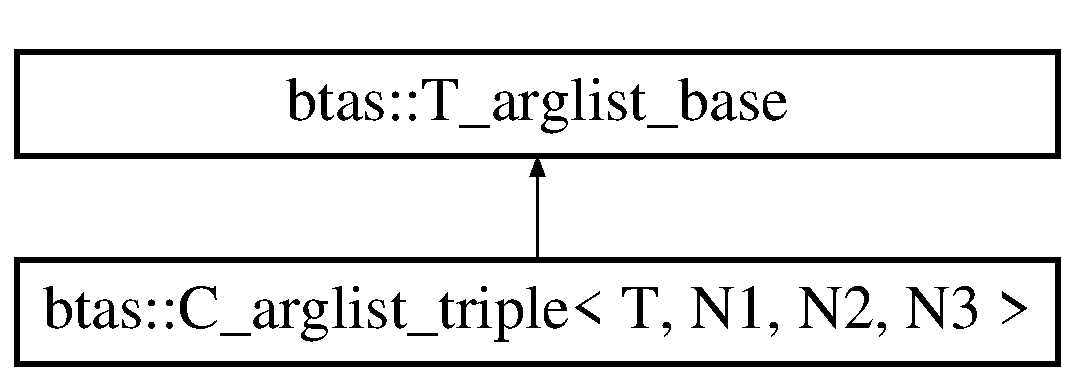
\includegraphics[height=2.000000cm]{d5/d67/classbtas_1_1C__arglist__triple}
\end{center}
\end{figure}
\subsection*{Public Member Functions}
\begin{DoxyCompactItemize}
\item 
{\bf C\-\_\-arglist\-\_\-triple} ()
\begin{DoxyCompactList}\small\item\em Default constructor. \end{DoxyCompactList}\item 
virtual {\bf $\sim$\-C\-\_\-arglist\-\_\-triple} ()
\begin{DoxyCompactList}\small\item\em Destructor. \end{DoxyCompactList}\item 
{\bf C\-\_\-arglist\-\_\-triple} (const shared\-\_\-ptr$<$ {\bf T\-Array}$<$ T, N3 $>$$>$ \&arg3\-\_\-ptr)
\begin{DoxyCompactList}\small\item\em Initializer. \end{DoxyCompactList}\item 
void {\bf reset} (const shared\-\_\-ptr$<$ {\bf T\-Array}$<$ T, N3 $>$$>$ \&arg3\-\_\-ptr)
\begin{DoxyCompactList}\small\item\em Reset argment 3. \end{DoxyCompactList}\item 
virtual void {\bf clear} ()
\begin{DoxyCompactList}\small\item\em Clear argments. \end{DoxyCompactList}\item 
void {\bf add} (const shared\-\_\-ptr$<$ {\bf T\-Array}$<$ T, N1 $>$$>$ \&arg1\-\_\-ptr, const shared\-\_\-ptr$<$ {\bf T\-Array}$<$ T, N2 $>$$>$ \&arg2\-\_\-ptr)
\begin{DoxyCompactList}\small\item\em Add argment list. \end{DoxyCompactList}\item 
size\-\_\-t {\bf size} () const 
\begin{DoxyCompactList}\small\item\em Return number of argment list. \end{DoxyCompactList}\end{DoxyCompactItemize}
\subsection*{Protected Member Functions}
\begin{DoxyCompactItemize}
\item 
virtual size\-\_\-t {\bf mf\-\_\-flops\-\_\-count} (const shared\-\_\-ptr$<$ {\bf T\-Array}$<$ T, N1 $>$$>$ \&arg1\-\_\-ptr, const shared\-\_\-ptr$<$ {\bf T\-Array}$<$ T, N2 $>$$>$ \&arg2\-\_\-ptr)
\begin{DoxyCompactList}\small\item\em Function to compute F\-L\-O\-P\-S count. \end{DoxyCompactList}\end{DoxyCompactItemize}
\subsection*{Protected Attributes}
\begin{DoxyCompactItemize}
\item 
std\-::vector$<$ shared\-\_\-ptr\\*
$<$ {\bf T\-Array}$<$ T, N1 $>$ $>$ $>$ {\bf m\-\_\-argment\-\_\-1}
\begin{DoxyCompactList}\small\item\em array list of a \end{DoxyCompactList}\item 
std\-::vector$<$ shared\-\_\-ptr\\*
$<$ {\bf T\-Array}$<$ T, N2 $>$ $>$ $>$ {\bf m\-\_\-argment\-\_\-2}
\begin{DoxyCompactList}\small\item\em array list of b \end{DoxyCompactList}\item 
shared\-\_\-ptr$<$ {\bf T\-Array}$<$ T, N3 $>$ $>$ {\bf m\-\_\-argment\-\_\-3}
\end{DoxyCompactItemize}


\subsection{Detailed Description}
\subsubsection*{template$<$typename T, size\-\_\-t N1, size\-\_\-t N2, size\-\_\-t N3$>$class btas\-::\-C\-\_\-arglist\-\_\-triple$<$ T, N1, N2, N3 $>$}

Argment list for contraction. 

i.\-e. B\-L\-A\-S (level 2, 3)\-: G\-E\-M\-V, G\-E\-R, G\-E\-M\-M, etc. m\-\_\-arglist has pairs of array (a, b) and m\-\_\-c\-\_\-ptr has the pointer to array (c), for function call s.\-t. c = sum\-\_\-\{i\} foo(a[i], b[i]) 

Definition at line 199 of file Targlist.\-h.



\subsection{Constructor \& Destructor Documentation}
\index{btas\-::\-C\-\_\-arglist\-\_\-triple@{btas\-::\-C\-\_\-arglist\-\_\-triple}!C\-\_\-arglist\-\_\-triple@{C\-\_\-arglist\-\_\-triple}}
\index{C\-\_\-arglist\-\_\-triple@{C\-\_\-arglist\-\_\-triple}!btas::C_arglist_triple@{btas\-::\-C\-\_\-arglist\-\_\-triple}}
\subsubsection[{C\-\_\-arglist\-\_\-triple}]{\setlength{\rightskip}{0pt plus 5cm}template$<$typename T, size\-\_\-t N1, size\-\_\-t N2, size\-\_\-t N3$>$ {\bf btas\-::\-C\-\_\-arglist\-\_\-triple}$<$ T, N1, N2, N3 $>$\-::{\bf C\-\_\-arglist\-\_\-triple} (
\begin{DoxyParamCaption}
{}
\end{DoxyParamCaption}
)\hspace{0.3cm}{\ttfamily [inline]}}\label{d5/d67/classbtas_1_1C__arglist__triple_a9dd4f5796599deab42425a15c4393b5b}


Default constructor. 



Definition at line 210 of file Targlist.\-h.

\index{btas\-::\-C\-\_\-arglist\-\_\-triple@{btas\-::\-C\-\_\-arglist\-\_\-triple}!$\sim$\-C\-\_\-arglist\-\_\-triple@{$\sim$\-C\-\_\-arglist\-\_\-triple}}
\index{$\sim$\-C\-\_\-arglist\-\_\-triple@{$\sim$\-C\-\_\-arglist\-\_\-triple}!btas::C_arglist_triple@{btas\-::\-C\-\_\-arglist\-\_\-triple}}
\subsubsection[{$\sim$\-C\-\_\-arglist\-\_\-triple}]{\setlength{\rightskip}{0pt plus 5cm}template$<$typename T, size\-\_\-t N1, size\-\_\-t N2, size\-\_\-t N3$>$ virtual {\bf btas\-::\-C\-\_\-arglist\-\_\-triple}$<$ T, N1, N2, N3 $>$\-::$\sim${\bf C\-\_\-arglist\-\_\-triple} (
\begin{DoxyParamCaption}
{}
\end{DoxyParamCaption}
)\hspace{0.3cm}{\ttfamily [inline]}, {\ttfamily [virtual]}}\label{d5/d67/classbtas_1_1C__arglist__triple_afee196154ed2b27e875161b132c5841b}


Destructor. 



Definition at line 212 of file Targlist.\-h.

\index{btas\-::\-C\-\_\-arglist\-\_\-triple@{btas\-::\-C\-\_\-arglist\-\_\-triple}!C\-\_\-arglist\-\_\-triple@{C\-\_\-arglist\-\_\-triple}}
\index{C\-\_\-arglist\-\_\-triple@{C\-\_\-arglist\-\_\-triple}!btas::C_arglist_triple@{btas\-::\-C\-\_\-arglist\-\_\-triple}}
\subsubsection[{C\-\_\-arglist\-\_\-triple}]{\setlength{\rightskip}{0pt plus 5cm}template$<$typename T, size\-\_\-t N1, size\-\_\-t N2, size\-\_\-t N3$>$ {\bf btas\-::\-C\-\_\-arglist\-\_\-triple}$<$ T, N1, N2, N3 $>$\-::{\bf C\-\_\-arglist\-\_\-triple} (
\begin{DoxyParamCaption}
\item[{const shared\-\_\-ptr$<$ {\bf T\-Array}$<$ T, N3 $>$$>$ \&}]{arg3\-\_\-ptr}
\end{DoxyParamCaption}
)\hspace{0.3cm}{\ttfamily [inline]}}\label{d5/d67/classbtas_1_1C__arglist__triple_a93a7ab93760d5f50ef53110c669f980b}


Initializer. 



Definition at line 215 of file Targlist.\-h.



\subsection{Member Function Documentation}
\index{btas\-::\-C\-\_\-arglist\-\_\-triple@{btas\-::\-C\-\_\-arglist\-\_\-triple}!add@{add}}
\index{add@{add}!btas::C_arglist_triple@{btas\-::\-C\-\_\-arglist\-\_\-triple}}
\subsubsection[{add}]{\setlength{\rightskip}{0pt plus 5cm}template$<$typename T, size\-\_\-t N1, size\-\_\-t N2, size\-\_\-t N3$>$ void {\bf btas\-::\-C\-\_\-arglist\-\_\-triple}$<$ T, N1, N2, N3 $>$\-::add (
\begin{DoxyParamCaption}
\item[{const shared\-\_\-ptr$<$ {\bf T\-Array}$<$ T, N1 $>$$>$ \&}]{arg1\-\_\-ptr, }
\item[{const shared\-\_\-ptr$<$ {\bf T\-Array}$<$ T, N2 $>$$>$ \&}]{arg2\-\_\-ptr}
\end{DoxyParamCaption}
)\hspace{0.3cm}{\ttfamily [inline]}}\label{d5/d67/classbtas_1_1C__arglist__triple_aedc2489b4d8f4a0d5ccb42db25397bc0}


Add argment list. 



Definition at line 231 of file Targlist.\-h.



Referenced by btas\-::\-Dgemv\-Arglist$<$ N\-A, N\-B, N\-C $>$\-::add(), btas\-::\-Dger\-Arglist$<$ N\-A, N\-B, N\-C $>$\-::add(), and btas\-::\-Dgemm\-Arglist$<$ N\-A, N\-B, N\-C $>$\-::add().

\index{btas\-::\-C\-\_\-arglist\-\_\-triple@{btas\-::\-C\-\_\-arglist\-\_\-triple}!clear@{clear}}
\index{clear@{clear}!btas::C_arglist_triple@{btas\-::\-C\-\_\-arglist\-\_\-triple}}
\subsubsection[{clear}]{\setlength{\rightskip}{0pt plus 5cm}template$<$typename T, size\-\_\-t N1, size\-\_\-t N2, size\-\_\-t N3$>$ virtual void {\bf btas\-::\-C\-\_\-arglist\-\_\-triple}$<$ T, N1, N2, N3 $>$\-::clear (
\begin{DoxyParamCaption}
{}
\end{DoxyParamCaption}
)\hspace{0.3cm}{\ttfamily [inline]}, {\ttfamily [virtual]}}\label{d5/d67/classbtas_1_1C__arglist__triple_a2df507deb003fe1a16a692dd76a408c5}


Clear argments. 



Reimplemented in {\bf btas\-::\-Dgemm\-Arglist$<$ N\-A, N\-B, N\-C $>$} \doxyref{}{p.}{d6/d9b/classbtas_1_1DgemmArglist_a90f7f0bf9d8e6cedb8eb1c2bf84b257e}, {\bf btas\-::\-Dger\-Arglist$<$ N\-A, N\-B, N\-C $>$} \doxyref{}{p.}{da/db6/classbtas_1_1DgerArglist_a43a8a8922741041d0724da534ccf866b}, and {\bf btas\-::\-Dgemv\-Arglist$<$ N\-A, N\-B, N\-C $>$} \doxyref{}{p.}{df/d7c/classbtas_1_1DgemvArglist_a48b444eefcb720024388a39ce05a7b3a}.



Definition at line 223 of file Targlist.\-h.



Referenced by btas\-::\-Dgemv\-Arglist$<$ N\-A, N\-B, N\-C $>$\-::clear(), btas\-::\-Dger\-Arglist$<$ N\-A, N\-B, N\-C $>$\-::clear(), and btas\-::\-Dgemm\-Arglist$<$ N\-A, N\-B, N\-C $>$\-::clear().

\index{btas\-::\-C\-\_\-arglist\-\_\-triple@{btas\-::\-C\-\_\-arglist\-\_\-triple}!mf\-\_\-flops\-\_\-count@{mf\-\_\-flops\-\_\-count}}
\index{mf\-\_\-flops\-\_\-count@{mf\-\_\-flops\-\_\-count}!btas::C_arglist_triple@{btas\-::\-C\-\_\-arglist\-\_\-triple}}
\subsubsection[{mf\-\_\-flops\-\_\-count}]{\setlength{\rightskip}{0pt plus 5cm}template$<$typename T, size\-\_\-t N1, size\-\_\-t N2, size\-\_\-t N3$>$ virtual size\-\_\-t {\bf btas\-::\-C\-\_\-arglist\-\_\-triple}$<$ T, N1, N2, N3 $>$\-::mf\-\_\-flops\-\_\-count (
\begin{DoxyParamCaption}
\item[{const shared\-\_\-ptr$<$ {\bf T\-Array}$<$ T, N1 $>$$>$ \&}]{arg1\-\_\-ptr, }
\item[{const shared\-\_\-ptr$<$ {\bf T\-Array}$<$ T, N2 $>$$>$ \&}]{arg2\-\_\-ptr}
\end{DoxyParamCaption}
)\hspace{0.3cm}{\ttfamily [inline]}, {\ttfamily [protected]}, {\ttfamily [virtual]}}\label{d5/d67/classbtas_1_1C__arglist__triple_a77718d56f71d6ae94dfab282c2bbe821}


Function to compute F\-L\-O\-P\-S count. 



Definition at line 206 of file Targlist.\-h.



Referenced by btas\-::\-C\-\_\-arglist\-\_\-triple$<$ double, N\-A, N\-B, N\-C $>$\-::add().

\index{btas\-::\-C\-\_\-arglist\-\_\-triple@{btas\-::\-C\-\_\-arglist\-\_\-triple}!reset@{reset}}
\index{reset@{reset}!btas::C_arglist_triple@{btas\-::\-C\-\_\-arglist\-\_\-triple}}
\subsubsection[{reset}]{\setlength{\rightskip}{0pt plus 5cm}template$<$typename T, size\-\_\-t N1, size\-\_\-t N2, size\-\_\-t N3$>$ void {\bf btas\-::\-C\-\_\-arglist\-\_\-triple}$<$ T, N1, N2, N3 $>$\-::reset (
\begin{DoxyParamCaption}
\item[{const shared\-\_\-ptr$<$ {\bf T\-Array}$<$ T, N3 $>$$>$ \&}]{arg3\-\_\-ptr}
\end{DoxyParamCaption}
)\hspace{0.3cm}{\ttfamily [inline]}}\label{d5/d67/classbtas_1_1C__arglist__triple_a1f3dd8710628e9e02aa6923e9d452297}


Reset argment 3. 



Definition at line 219 of file Targlist.\-h.



Referenced by btas\-::\-Dgemv\-Arglist$<$ N\-A, N\-B, N\-C $>$\-::reset(), btas\-::\-Dger\-Arglist$<$ N\-A, N\-B, N\-C $>$\-::reset(), and btas\-::\-Dgemm\-Arglist$<$ N\-A, N\-B, N\-C $>$\-::reset().

\index{btas\-::\-C\-\_\-arglist\-\_\-triple@{btas\-::\-C\-\_\-arglist\-\_\-triple}!size@{size}}
\index{size@{size}!btas::C_arglist_triple@{btas\-::\-C\-\_\-arglist\-\_\-triple}}
\subsubsection[{size}]{\setlength{\rightskip}{0pt plus 5cm}template$<$typename T, size\-\_\-t N1, size\-\_\-t N2, size\-\_\-t N3$>$ size\-\_\-t {\bf btas\-::\-C\-\_\-arglist\-\_\-triple}$<$ T, N1, N2, N3 $>$\-::size (
\begin{DoxyParamCaption}
{}
\end{DoxyParamCaption}
) const\hspace{0.3cm}{\ttfamily [inline]}}\label{d5/d67/classbtas_1_1C__arglist__triple_a671322982551a4eb2a6acc70978dd634}


Return number of argment list. 



Definition at line 238 of file Targlist.\-h.



\subsection{Field Documentation}
\index{btas\-::\-C\-\_\-arglist\-\_\-triple@{btas\-::\-C\-\_\-arglist\-\_\-triple}!m\-\_\-argment\-\_\-1@{m\-\_\-argment\-\_\-1}}
\index{m\-\_\-argment\-\_\-1@{m\-\_\-argment\-\_\-1}!btas::C_arglist_triple@{btas\-::\-C\-\_\-arglist\-\_\-triple}}
\subsubsection[{m\-\_\-argment\-\_\-1}]{\setlength{\rightskip}{0pt plus 5cm}template$<$typename T, size\-\_\-t N1, size\-\_\-t N2, size\-\_\-t N3$>$ std\-::vector$<$shared\-\_\-ptr$<${\bf T\-Array}$<$T, N1$>$ $>$ $>$ {\bf btas\-::\-C\-\_\-arglist\-\_\-triple}$<$ T, N1, N2, N3 $>$\-::m\-\_\-argment\-\_\-1\hspace{0.3cm}{\ttfamily [protected]}}\label{d5/d67/classbtas_1_1C__arglist__triple_ab64e5b37ac2e4cf445699718b42bd097}


array list of a 



Definition at line 201 of file Targlist.\-h.



Referenced by btas\-::\-C\-\_\-arglist\-\_\-triple$<$ double, N\-A, N\-B, N\-C $>$\-::add(), btas\-::\-C\-\_\-arglist\-\_\-triple$<$ double, N\-A, N\-B, N\-C $>$\-::clear(), and btas\-::\-C\-\_\-arglist\-\_\-triple$<$ double, N\-A, N\-B, N\-C $>$\-::size().

\index{btas\-::\-C\-\_\-arglist\-\_\-triple@{btas\-::\-C\-\_\-arglist\-\_\-triple}!m\-\_\-argment\-\_\-2@{m\-\_\-argment\-\_\-2}}
\index{m\-\_\-argment\-\_\-2@{m\-\_\-argment\-\_\-2}!btas::C_arglist_triple@{btas\-::\-C\-\_\-arglist\-\_\-triple}}
\subsubsection[{m\-\_\-argment\-\_\-2}]{\setlength{\rightskip}{0pt plus 5cm}template$<$typename T, size\-\_\-t N1, size\-\_\-t N2, size\-\_\-t N3$>$ std\-::vector$<$shared\-\_\-ptr$<${\bf T\-Array}$<$T, N2$>$ $>$ $>$ {\bf btas\-::\-C\-\_\-arglist\-\_\-triple}$<$ T, N1, N2, N3 $>$\-::m\-\_\-argment\-\_\-2\hspace{0.3cm}{\ttfamily [protected]}}\label{d5/d67/classbtas_1_1C__arglist__triple_aa63ab62d457b84c9e7237a7943481220}


array list of b 



Definition at line 202 of file Targlist.\-h.



Referenced by btas\-::\-C\-\_\-arglist\-\_\-triple$<$ double, N\-A, N\-B, N\-C $>$\-::add(), and btas\-::\-C\-\_\-arglist\-\_\-triple$<$ double, N\-A, N\-B, N\-C $>$\-::clear().

\index{btas\-::\-C\-\_\-arglist\-\_\-triple@{btas\-::\-C\-\_\-arglist\-\_\-triple}!m\-\_\-argment\-\_\-3@{m\-\_\-argment\-\_\-3}}
\index{m\-\_\-argment\-\_\-3@{m\-\_\-argment\-\_\-3}!btas::C_arglist_triple@{btas\-::\-C\-\_\-arglist\-\_\-triple}}
\subsubsection[{m\-\_\-argment\-\_\-3}]{\setlength{\rightskip}{0pt plus 5cm}template$<$typename T, size\-\_\-t N1, size\-\_\-t N2, size\-\_\-t N3$>$ shared\-\_\-ptr$<${\bf T\-Array}$<$T, N3$>$ $>$ {\bf btas\-::\-C\-\_\-arglist\-\_\-triple}$<$ T, N1, N2, N3 $>$\-::m\-\_\-argment\-\_\-3\hspace{0.3cm}{\ttfamily [protected]}}\label{d5/d67/classbtas_1_1C__arglist__triple_ae135b1e690b14b78d69272c6d45f6833}
array c 

Definition at line 203 of file Targlist.\-h.



Referenced by btas\-::\-C\-\_\-arglist\-\_\-triple$<$ double, N\-A, N\-B, N\-C $>$\-::clear(), btas\-::\-C\-\_\-arglist\-\_\-triple$<$ double, N\-A, N\-B, N\-C $>$\-::mf\-\_\-flops\-\_\-count(), and btas\-::\-C\-\_\-arglist\-\_\-triple$<$ double, N\-A, N\-B, N\-C $>$\-::reset().



The documentation for this class was generated from the following file\-:\begin{DoxyCompactItemize}
\item 
include/btas/{\bf Targlist.\-h}\end{DoxyCompactItemize}

\section{btas\-:\-:Daxpy\-Arglist$<$ N $>$ Class Template Reference}
\label{d3/d12/classbtas_1_1DaxpyArglist}\index{btas\-::\-Daxpy\-Arglist$<$ N $>$@{btas\-::\-Daxpy\-Arglist$<$ N $>$}}


{\ttfamily \#include $<$Darglist.\-h$>$}

Inheritance diagram for btas\-:\-:Daxpy\-Arglist$<$ N $>$\-:\begin{figure}[H]
\begin{center}
\leavevmode
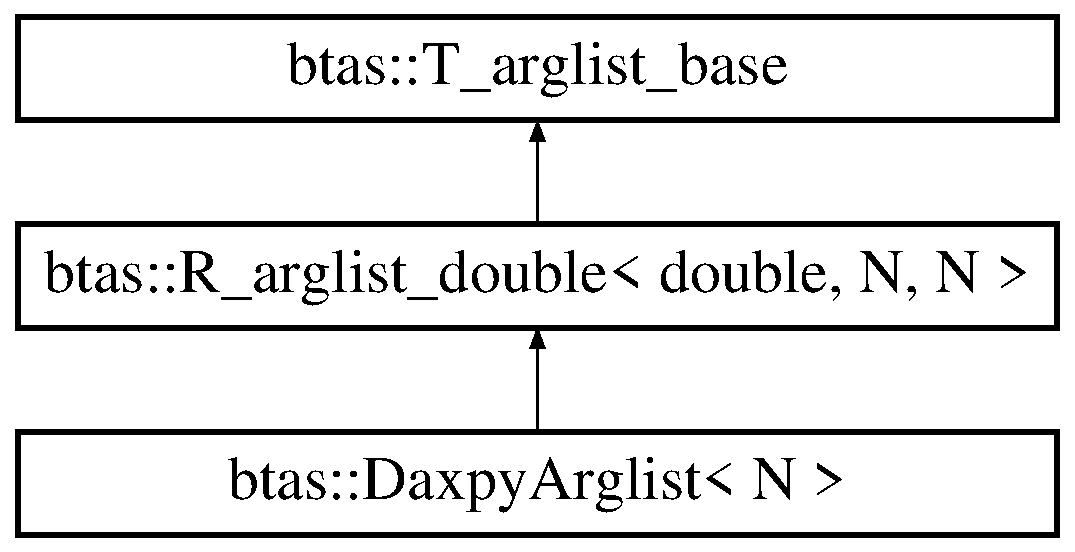
\includegraphics[height=3.000000cm]{d3/d12/classbtas_1_1DaxpyArglist}
\end{center}
\end{figure}
\subsection*{Public Member Functions}
\begin{DoxyCompactItemize}
\item 
{\bf Daxpy\-Arglist} ()
\begin{DoxyCompactList}\small\item\em Default constructor. \end{DoxyCompactList}\item 
{\bf Daxpy\-Arglist} (const double \&alpha, const shared\-\_\-ptr$<$ {\bf D\-Array}$<$ N $>$$>$ \&x\-\_\-ptr, const shared\-\_\-ptr$<$ {\bf D\-Array}$<$ N $>$$>$ \&y\-\_\-ptr)
\begin{DoxyCompactList}\small\item\em Initializer. \end{DoxyCompactList}\item 
void {\bf reset} (const double \&alpha, const shared\-\_\-ptr$<$ {\bf D\-Array}$<$ N $>$$>$ \&x\-\_\-ptr, const shared\-\_\-ptr$<$ {\bf D\-Array}$<$ N $>$$>$ \&y\-\_\-ptr)
\begin{DoxyCompactList}\small\item\em Reset arglist. \end{DoxyCompactList}\item 
void {\bf call} () const 
\begin{DoxyCompactList}\small\item\em Call Daxpy. \end{DoxyCompactList}\end{DoxyCompactItemize}
\subsection*{Private Attributes}
\begin{DoxyCompactItemize}
\item 
double {\bf m\-\_\-alpha}
\end{DoxyCompactItemize}
\subsection*{Additional Inherited Members}


\subsection{Detailed Description}
\subsubsection*{template$<$size\-\_\-t N$>$class btas\-::\-Daxpy\-Arglist$<$ N $>$}



Definition at line 59 of file Darglist.\-h.



\subsection{Constructor \& Destructor Documentation}
\index{btas\-::\-Daxpy\-Arglist@{btas\-::\-Daxpy\-Arglist}!Daxpy\-Arglist@{Daxpy\-Arglist}}
\index{Daxpy\-Arglist@{Daxpy\-Arglist}!btas::DaxpyArglist@{btas\-::\-Daxpy\-Arglist}}
\subsubsection[{Daxpy\-Arglist}]{\setlength{\rightskip}{0pt plus 5cm}template$<$size\-\_\-t N$>$ {\bf btas\-::\-Daxpy\-Arglist}$<$ N $>$\-::{\bf Daxpy\-Arglist} (
\begin{DoxyParamCaption}
{}
\end{DoxyParamCaption}
)\hspace{0.3cm}{\ttfamily [inline]}}\label{d3/d12/classbtas_1_1DaxpyArglist_ac9f68ced22d39c62c7e8737f57d66573}


Default constructor. 



Definition at line 65 of file Darglist.\-h.

\index{btas\-::\-Daxpy\-Arglist@{btas\-::\-Daxpy\-Arglist}!Daxpy\-Arglist@{Daxpy\-Arglist}}
\index{Daxpy\-Arglist@{Daxpy\-Arglist}!btas::DaxpyArglist@{btas\-::\-Daxpy\-Arglist}}
\subsubsection[{Daxpy\-Arglist}]{\setlength{\rightskip}{0pt plus 5cm}template$<$size\-\_\-t N$>$ {\bf btas\-::\-Daxpy\-Arglist}$<$ N $>$\-::{\bf Daxpy\-Arglist} (
\begin{DoxyParamCaption}
\item[{const double \&}]{alpha, }
\item[{const shared\-\_\-ptr$<$ {\bf D\-Array}$<$ N $>$$>$ \&}]{x\-\_\-ptr, }
\item[{const shared\-\_\-ptr$<$ {\bf D\-Array}$<$ N $>$$>$ \&}]{y\-\_\-ptr}
\end{DoxyParamCaption}
)\hspace{0.3cm}{\ttfamily [inline]}}\label{d3/d12/classbtas_1_1DaxpyArglist_ae4dd3c60303e5927a266becec781d96d}


Initializer. 



Definition at line 68 of file Darglist.\-h.



\subsection{Member Function Documentation}
\index{btas\-::\-Daxpy\-Arglist@{btas\-::\-Daxpy\-Arglist}!call@{call}}
\index{call@{call}!btas::DaxpyArglist@{btas\-::\-Daxpy\-Arglist}}
\subsubsection[{call}]{\setlength{\rightskip}{0pt plus 5cm}template$<$size\-\_\-t N$>$ void {\bf btas\-::\-Daxpy\-Arglist}$<$ N $>$\-::call (
\begin{DoxyParamCaption}
{}
\end{DoxyParamCaption}
) const\hspace{0.3cm}{\ttfamily [inline]}}\label{d3/d12/classbtas_1_1DaxpyArglist_a0a73ba4569447d3dcff588f2949b58c9}


Call Daxpy. 



Definition at line 81 of file Darglist.\-h.



References btas\-::\-Daxpy(), and btas\-::\-Daxpy\-Arglist$<$ N $>$\-::m\-\_\-alpha.

\index{btas\-::\-Daxpy\-Arglist@{btas\-::\-Daxpy\-Arglist}!reset@{reset}}
\index{reset@{reset}!btas::DaxpyArglist@{btas\-::\-Daxpy\-Arglist}}
\subsubsection[{reset}]{\setlength{\rightskip}{0pt plus 5cm}template$<$size\-\_\-t N$>$ void {\bf btas\-::\-Daxpy\-Arglist}$<$ N $>$\-::reset (
\begin{DoxyParamCaption}
\item[{const double \&}]{alpha, }
\item[{const shared\-\_\-ptr$<$ {\bf D\-Array}$<$ N $>$$>$ \&}]{x\-\_\-ptr, }
\item[{const shared\-\_\-ptr$<$ {\bf D\-Array}$<$ N $>$$>$ \&}]{y\-\_\-ptr}
\end{DoxyParamCaption}
)\hspace{0.3cm}{\ttfamily [inline]}}\label{d3/d12/classbtas_1_1DaxpyArglist_ae60c31b163bddc69ea24db1e3fe513a0}


Reset arglist. 



Definition at line 74 of file Darglist.\-h.



References btas\-::\-Daxpy\-Arglist$<$ N $>$\-::m\-\_\-alpha, and btas\-::\-R\-\_\-arglist\-\_\-double$<$ T, N1, N2 $>$\-::reset().



\subsection{Field Documentation}
\index{btas\-::\-Daxpy\-Arglist@{btas\-::\-Daxpy\-Arglist}!m\-\_\-alpha@{m\-\_\-alpha}}
\index{m\-\_\-alpha@{m\-\_\-alpha}!btas::DaxpyArglist@{btas\-::\-Daxpy\-Arglist}}
\subsubsection[{m\-\_\-alpha}]{\setlength{\rightskip}{0pt plus 5cm}template$<$size\-\_\-t N$>$ double {\bf btas\-::\-Daxpy\-Arglist}$<$ N $>$\-::m\-\_\-alpha\hspace{0.3cm}{\ttfamily [private]}}\label{d3/d12/classbtas_1_1DaxpyArglist_a787baaae8e7bd6786246b87fa4ed3196}


Definition at line 62 of file Darglist.\-h.



Referenced by btas\-::\-Daxpy\-Arglist$<$ N $>$\-::call(), and btas\-::\-Daxpy\-Arglist$<$ N $>$\-::reset().



The documentation for this class was generated from the following file\-:\begin{DoxyCompactItemize}
\item 
include/btas/\-D\-E\-N\-S\-E/{\bf Darglist.\-h}\end{DoxyCompactItemize}

\section{btas\-:\-:Dcopy\-Arglist$<$ N $>$ Class Template Reference}
\label{d9/dfc/classbtas_1_1DcopyArglist}\index{btas\-::\-Dcopy\-Arglist$<$ N $>$@{btas\-::\-Dcopy\-Arglist$<$ N $>$}}


{\ttfamily \#include $<$Darglist.\-h$>$}

Inheritance diagram for btas\-:\-:Dcopy\-Arglist$<$ N $>$\-:\begin{figure}[H]
\begin{center}
\leavevmode
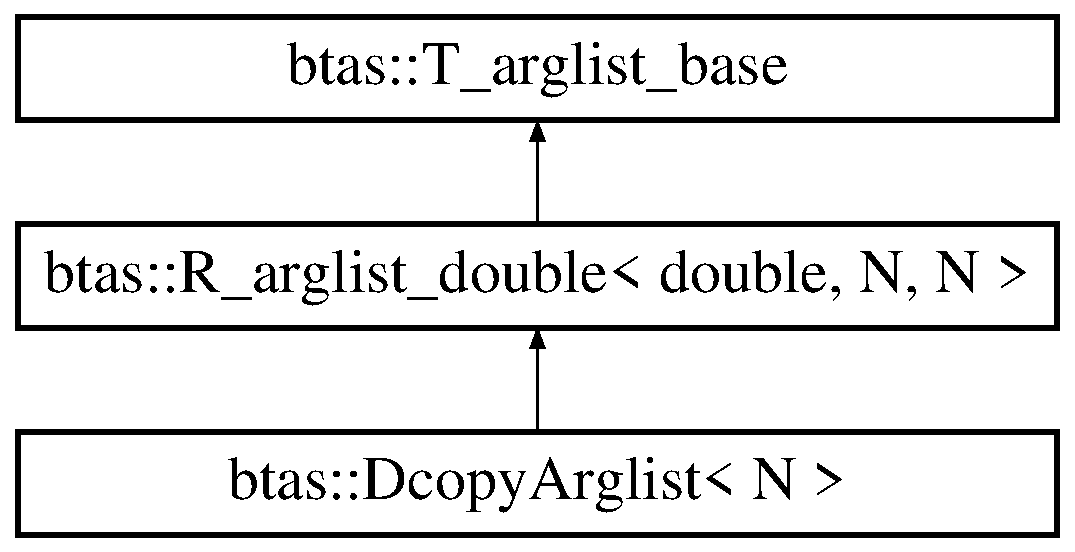
\includegraphics[height=3.000000cm]{d9/dfc/classbtas_1_1DcopyArglist}
\end{center}
\end{figure}
\subsection*{Public Member Functions}
\begin{DoxyCompactItemize}
\item 
{\bf Dcopy\-Arglist} ()
\begin{DoxyCompactList}\small\item\em Default constructor. \end{DoxyCompactList}\item 
{\bf Dcopy\-Arglist} (const shared\-\_\-ptr$<$ {\bf D\-Array}$<$ N $>$$>$ \&x\-\_\-ptr, const shared\-\_\-ptr$<$ {\bf D\-Array}$<$ N $>$$>$ \&y\-\_\-ptr)
\begin{DoxyCompactList}\small\item\em Initializer. \end{DoxyCompactList}\item 
void {\bf call} () const 
\begin{DoxyCompactList}\small\item\em Call Dcopy. \end{DoxyCompactList}\end{DoxyCompactItemize}
\subsection*{Additional Inherited Members}


\subsection{Detailed Description}
\subsubsection*{template$<$size\-\_\-t N$>$class btas\-::\-Dcopy\-Arglist$<$ N $>$}



Definition at line 20 of file Darglist.\-h.



\subsection{Constructor \& Destructor Documentation}
\index{btas\-::\-Dcopy\-Arglist@{btas\-::\-Dcopy\-Arglist}!Dcopy\-Arglist@{Dcopy\-Arglist}}
\index{Dcopy\-Arglist@{Dcopy\-Arglist}!btas::DcopyArglist@{btas\-::\-Dcopy\-Arglist}}
\subsubsection[{Dcopy\-Arglist}]{\setlength{\rightskip}{0pt plus 5cm}template$<$size\-\_\-t N$>$ {\bf btas\-::\-Dcopy\-Arglist}$<$ N $>$\-::{\bf Dcopy\-Arglist} (
\begin{DoxyParamCaption}
{}
\end{DoxyParamCaption}
)\hspace{0.3cm}{\ttfamily [inline]}}\label{d9/dfc/classbtas_1_1DcopyArglist_aef87db883b5ac4f14323e565f89101e6}


Default constructor. 



Definition at line 23 of file Darglist.\-h.

\index{btas\-::\-Dcopy\-Arglist@{btas\-::\-Dcopy\-Arglist}!Dcopy\-Arglist@{Dcopy\-Arglist}}
\index{Dcopy\-Arglist@{Dcopy\-Arglist}!btas::DcopyArglist@{btas\-::\-Dcopy\-Arglist}}
\subsubsection[{Dcopy\-Arglist}]{\setlength{\rightskip}{0pt plus 5cm}template$<$size\-\_\-t N$>$ {\bf btas\-::\-Dcopy\-Arglist}$<$ N $>$\-::{\bf Dcopy\-Arglist} (
\begin{DoxyParamCaption}
\item[{const shared\-\_\-ptr$<$ {\bf D\-Array}$<$ N $>$$>$ \&}]{x\-\_\-ptr, }
\item[{const shared\-\_\-ptr$<$ {\bf D\-Array}$<$ N $>$$>$ \&}]{y\-\_\-ptr}
\end{DoxyParamCaption}
)\hspace{0.3cm}{\ttfamily [inline]}}\label{d9/dfc/classbtas_1_1DcopyArglist_af9563cf4f09d3bdbb81ed557c21ca32d}


Initializer. 



Definition at line 26 of file Darglist.\-h.



\subsection{Member Function Documentation}
\index{btas\-::\-Dcopy\-Arglist@{btas\-::\-Dcopy\-Arglist}!call@{call}}
\index{call@{call}!btas::DcopyArglist@{btas\-::\-Dcopy\-Arglist}}
\subsubsection[{call}]{\setlength{\rightskip}{0pt plus 5cm}template$<$size\-\_\-t N$>$ void {\bf btas\-::\-Dcopy\-Arglist}$<$ N $>$\-::call (
\begin{DoxyParamCaption}
{}
\end{DoxyParamCaption}
) const\hspace{0.3cm}{\ttfamily [inline]}}\label{d9/dfc/classbtas_1_1DcopyArglist_a203dbe487df96f6d57b672eb392a5e71}


Call Dcopy. 



Definition at line 30 of file Darglist.\-h.



References btas\-::\-Dcopy().



The documentation for this class was generated from the following file\-:\begin{DoxyCompactItemize}
\item 
include/btas/\-D\-E\-N\-S\-E/{\bf Darglist.\-h}\end{DoxyCompactItemize}

\section{btas\-:\-:Dgemm\-Arglist$<$ N\-A, N\-B, N\-C $>$ Class Template Reference}
\label{d6/d9b/classbtas_1_1DgemmArglist}\index{btas\-::\-Dgemm\-Arglist$<$ N\-A, N\-B, N\-C $>$@{btas\-::\-Dgemm\-Arglist$<$ N\-A, N\-B, N\-C $>$}}


{\ttfamily \#include $<$Darglist.\-h$>$}

Inheritance diagram for btas\-:\-:Dgemm\-Arglist$<$ N\-A, N\-B, N\-C $>$\-:\begin{figure}[H]
\begin{center}
\leavevmode
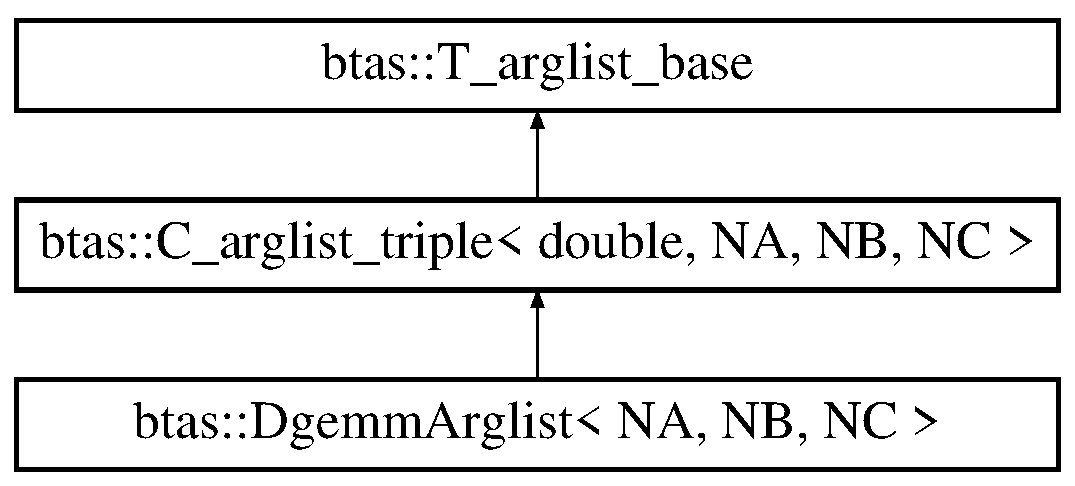
\includegraphics[height=3.000000cm]{d6/d9b/classbtas_1_1DgemmArglist}
\end{center}
\end{figure}
\subsection*{Public Member Functions}
\begin{DoxyCompactItemize}
\item 
{\bf Dgemm\-Arglist} ()
\begin{DoxyCompactList}\small\item\em Default constructor. \end{DoxyCompactList}\item 
{\bf Dgemm\-Arglist} (const shared\-\_\-ptr$<$ {\bf D\-Array}$<$ N\-C $>$$>$ \&c\-\_\-ptr, const {\bf B\-T\-A\-S\-\_\-\-T\-R\-A\-N\-S\-P\-O\-S\-E} \&transa={\bf No\-Trans}, const {\bf B\-T\-A\-S\-\_\-\-T\-R\-A\-N\-S\-P\-O\-S\-E} \&transb={\bf No\-Trans}, const double \&alpha=1.\-0, const double \&beta=1.\-0)
\begin{DoxyCompactList}\small\item\em Initializer. \end{DoxyCompactList}\item 
void {\bf reset} (const shared\-\_\-ptr$<$ {\bf D\-Array}$<$ N\-C $>$$>$ \&c\-\_\-ptr, const {\bf B\-T\-A\-S\-\_\-\-T\-R\-A\-N\-S\-P\-O\-S\-E} \&transa={\bf No\-Trans}, const {\bf B\-T\-A\-S\-\_\-\-T\-R\-A\-N\-S\-P\-O\-S\-E} \&transb={\bf No\-Trans}, const double \&alpha=1.\-0, const double \&beta=1.\-0)
\begin{DoxyCompactList}\small\item\em Reset arglist. \end{DoxyCompactList}\item 
void {\bf clear} ()
\begin{DoxyCompactList}\small\item\em Clear argments. \end{DoxyCompactList}\item 
void {\bf add} (const shared\-\_\-ptr$<$ {\bf D\-Array}$<$ N\-A $>$$>$ \&a\-\_\-ptr, const shared\-\_\-ptr$<$ {\bf D\-Array}$<$ N\-B $>$$>$ \&b\-\_\-ptr, double scale=1.\-0)
\begin{DoxyCompactList}\small\item\em Add arglist. \end{DoxyCompactList}\item 
void {\bf call} () const 
\begin{DoxyCompactList}\small\item\em Call Dgemm. \end{DoxyCompactList}\end{DoxyCompactItemize}
\subsection*{Private Member Functions}
\begin{DoxyCompactItemize}
\item 
size\-\_\-t {\bf mf\-\_\-flops\-\_\-count} (const shared\-\_\-ptr$<$ {\bf D\-Array}$<$ N\-A $>$$>$ \&a\-\_\-ptr, const shared\-\_\-ptr$<$ {\bf D\-Array}$<$ N\-B $>$$>$ \&b\-\_\-ptr)
\begin{DoxyCompactList}\small\item\em return F\-L\-O\-P\-S count \end{DoxyCompactList}\end{DoxyCompactItemize}
\subsection*{Private Attributes}
\begin{DoxyCompactItemize}
\item 
std\-::vector$<$ double $>$ {\bf m\-\_\-scale}
\begin{DoxyCompactList}\small\item\em this contains index-\/dependent scaling s.\-t. parity, Clebsch-\/\-Gordan coeff., etc. \end{DoxyCompactList}\item 
{\bf B\-T\-A\-S\-\_\-\-T\-R\-A\-N\-S\-P\-O\-S\-E} {\bf m\-\_\-transa}
\item 
{\bf B\-T\-A\-S\-\_\-\-T\-R\-A\-N\-S\-P\-O\-S\-E} {\bf m\-\_\-transb}
\item 
double {\bf m\-\_\-alpha}
\item 
double {\bf m\-\_\-beta}
\end{DoxyCompactItemize}
\subsection*{Additional Inherited Members}


\subsection{Detailed Description}
\subsubsection*{template$<$size\-\_\-t N\-A, size\-\_\-t N\-B, size\-\_\-t N\-C$>$class btas\-::\-Dgemm\-Arglist$<$ N\-A, N\-B, N\-C $>$}



Definition at line 230 of file Darglist.\-h.



\subsection{Constructor \& Destructor Documentation}
\index{btas\-::\-Dgemm\-Arglist@{btas\-::\-Dgemm\-Arglist}!Dgemm\-Arglist@{Dgemm\-Arglist}}
\index{Dgemm\-Arglist@{Dgemm\-Arglist}!btas::DgemmArglist@{btas\-::\-Dgemm\-Arglist}}
\subsubsection[{Dgemm\-Arglist}]{\setlength{\rightskip}{0pt plus 5cm}template$<$size\-\_\-t N\-A, size\-\_\-t N\-B, size\-\_\-t N\-C$>$ {\bf btas\-::\-Dgemm\-Arglist}$<$ N\-A, N\-B, N\-C $>$\-::{\bf Dgemm\-Arglist} (
\begin{DoxyParamCaption}
{}
\end{DoxyParamCaption}
)\hspace{0.3cm}{\ttfamily [inline]}}\label{d6/d9b/classbtas_1_1DgemmArglist_a0fd868f66d8e27932f4ee9857f27bd3d}


Default constructor. 



Definition at line 260 of file Darglist.\-h.

\index{btas\-::\-Dgemm\-Arglist@{btas\-::\-Dgemm\-Arglist}!Dgemm\-Arglist@{Dgemm\-Arglist}}
\index{Dgemm\-Arglist@{Dgemm\-Arglist}!btas::DgemmArglist@{btas\-::\-Dgemm\-Arglist}}
\subsubsection[{Dgemm\-Arglist}]{\setlength{\rightskip}{0pt plus 5cm}template$<$size\-\_\-t N\-A, size\-\_\-t N\-B, size\-\_\-t N\-C$>$ {\bf btas\-::\-Dgemm\-Arglist}$<$ N\-A, N\-B, N\-C $>$\-::{\bf Dgemm\-Arglist} (
\begin{DoxyParamCaption}
\item[{const shared\-\_\-ptr$<$ {\bf D\-Array}$<$ N\-C $>$$>$ \&}]{c\-\_\-ptr, }
\item[{const {\bf B\-T\-A\-S\-\_\-\-T\-R\-A\-N\-S\-P\-O\-S\-E} \&}]{transa = {\ttfamily {\bf No\-Trans}}, }
\item[{const {\bf B\-T\-A\-S\-\_\-\-T\-R\-A\-N\-S\-P\-O\-S\-E} \&}]{transb = {\ttfamily {\bf No\-Trans}}, }
\item[{const double \&}]{alpha = {\ttfamily 1.0}, }
\item[{const double \&}]{beta = {\ttfamily 1.0}}
\end{DoxyParamCaption}
)\hspace{0.3cm}{\ttfamily [inline]}}\label{d6/d9b/classbtas_1_1DgemmArglist_aded7dcfb0a650c0238fbbad005499831}


Initializer. 



Definition at line 263 of file Darglist.\-h.



\subsection{Member Function Documentation}
\index{btas\-::\-Dgemm\-Arglist@{btas\-::\-Dgemm\-Arglist}!add@{add}}
\index{add@{add}!btas::DgemmArglist@{btas\-::\-Dgemm\-Arglist}}
\subsubsection[{add}]{\setlength{\rightskip}{0pt plus 5cm}template$<$size\-\_\-t N\-A, size\-\_\-t N\-B, size\-\_\-t N\-C$>$ void {\bf btas\-::\-Dgemm\-Arglist}$<$ N\-A, N\-B, N\-C $>$\-::add (
\begin{DoxyParamCaption}
\item[{const shared\-\_\-ptr$<$ {\bf D\-Array}$<$ N\-A $>$$>$ \&}]{a\-\_\-ptr, }
\item[{const shared\-\_\-ptr$<$ {\bf D\-Array}$<$ N\-B $>$$>$ \&}]{b\-\_\-ptr, }
\item[{double}]{scale = {\ttfamily 1.0}}
\end{DoxyParamCaption}
)\hspace{0.3cm}{\ttfamily [inline]}}\label{d6/d9b/classbtas_1_1DgemmArglist_a49343dc10366c1db2d2b524b798e23c2}


Add arglist. 



Definition at line 294 of file Darglist.\-h.



References btas\-::\-C\-\_\-arglist\-\_\-triple$<$ T, N1, N2, N3 $>$\-::add(), and btas\-::\-Dgemm\-Arglist$<$ N\-A, N\-B, N\-C $>$\-::m\-\_\-scale.



Referenced by btas\-::thread\-\_\-\-S\-Dgemm().

\index{btas\-::\-Dgemm\-Arglist@{btas\-::\-Dgemm\-Arglist}!call@{call}}
\index{call@{call}!btas::DgemmArglist@{btas\-::\-Dgemm\-Arglist}}
\subsubsection[{call}]{\setlength{\rightskip}{0pt plus 5cm}template$<$size\-\_\-t N\-A, size\-\_\-t N\-B, size\-\_\-t N\-C$>$ void {\bf btas\-::\-Dgemm\-Arglist}$<$ N\-A, N\-B, N\-C $>$\-::call (
\begin{DoxyParamCaption}
{}
\end{DoxyParamCaption}
) const\hspace{0.3cm}{\ttfamily [inline]}}\label{d6/d9b/classbtas_1_1DgemmArglist_a15537a90b45c2591f1d3defb17d91cc9}


Call Dgemm. 



Definition at line 300 of file Darglist.\-h.



References btas\-::\-Dgemm(), btas\-::\-Dgemm\-Arglist$<$ N\-A, N\-B, N\-C $>$\-::m\-\_\-alpha, btas\-::\-Dgemm\-Arglist$<$ N\-A, N\-B, N\-C $>$\-::m\-\_\-beta, btas\-::\-Dgemm\-Arglist$<$ N\-A, N\-B, N\-C $>$\-::m\-\_\-scale, btas\-::\-Dgemm\-Arglist$<$ N\-A, N\-B, N\-C $>$\-::m\-\_\-transa, btas\-::\-Dgemm\-Arglist$<$ N\-A, N\-B, N\-C $>$\-::m\-\_\-transb, and btas\-::\-C\-\_\-arglist\-\_\-triple$<$ double, N\-A, N\-B, N\-C $>$\-::size().

\index{btas\-::\-Dgemm\-Arglist@{btas\-::\-Dgemm\-Arglist}!clear@{clear}}
\index{clear@{clear}!btas::DgemmArglist@{btas\-::\-Dgemm\-Arglist}}
\subsubsection[{clear}]{\setlength{\rightskip}{0pt plus 5cm}template$<$size\-\_\-t N\-A, size\-\_\-t N\-B, size\-\_\-t N\-C$>$ void {\bf btas\-::\-Dgemm\-Arglist}$<$ N\-A, N\-B, N\-C $>$\-::clear (
\begin{DoxyParamCaption}
{}
\end{DoxyParamCaption}
)\hspace{0.3cm}{\ttfamily [inline]}, {\ttfamily [virtual]}}\label{d6/d9b/classbtas_1_1DgemmArglist_a90f7f0bf9d8e6cedb8eb1c2bf84b257e}


Clear argments. 



Reimplemented from {\bf btas\-::\-C\-\_\-arglist\-\_\-triple$<$ double, N\-A, N\-B, N\-C $>$} \doxyref{}{p.}{d5/d67/classbtas_1_1C__arglist__triple_a2df507deb003fe1a16a692dd76a408c5}.



Definition at line 284 of file Darglist.\-h.



References btas\-::\-C\-\_\-arglist\-\_\-triple$<$ T, N1, N2, N3 $>$\-::clear(), btas\-::\-Dgemm\-Arglist$<$ N\-A, N\-B, N\-C $>$\-::m\-\_\-alpha, btas\-::\-Dgemm\-Arglist$<$ N\-A, N\-B, N\-C $>$\-::m\-\_\-beta, btas\-::\-Dgemm\-Arglist$<$ N\-A, N\-B, N\-C $>$\-::m\-\_\-scale, btas\-::\-Dgemm\-Arglist$<$ N\-A, N\-B, N\-C $>$\-::m\-\_\-transa, btas\-::\-Dgemm\-Arglist$<$ N\-A, N\-B, N\-C $>$\-::m\-\_\-transb, and btas\-::\-No\-Trans.

\index{btas\-::\-Dgemm\-Arglist@{btas\-::\-Dgemm\-Arglist}!mf\-\_\-flops\-\_\-count@{mf\-\_\-flops\-\_\-count}}
\index{mf\-\_\-flops\-\_\-count@{mf\-\_\-flops\-\_\-count}!btas::DgemmArglist@{btas\-::\-Dgemm\-Arglist}}
\subsubsection[{mf\-\_\-flops\-\_\-count}]{\setlength{\rightskip}{0pt plus 5cm}template$<$size\-\_\-t N\-A, size\-\_\-t N\-B, size\-\_\-t N\-C$>$ size\-\_\-t {\bf btas\-::\-Dgemm\-Arglist}$<$ N\-A, N\-B, N\-C $>$\-::mf\-\_\-flops\-\_\-count (
\begin{DoxyParamCaption}
\item[{const shared\-\_\-ptr$<$ {\bf D\-Array}$<$ N\-A $>$$>$ \&}]{a\-\_\-ptr, }
\item[{const shared\-\_\-ptr$<$ {\bf D\-Array}$<$ N\-B $>$$>$ \&}]{b\-\_\-ptr}
\end{DoxyParamCaption}
)\hspace{0.3cm}{\ttfamily [inline]}, {\ttfamily [private]}}\label{d6/d9b/classbtas_1_1DgemmArglist_a6dfdf7a21991773cf0c5b02dd8bb0ea7}


return F\-L\-O\-P\-S count 



Definition at line 245 of file Darglist.\-h.



References btas\-::\-Dgemm\-Arglist$<$ N\-A, N\-B, N\-C $>$\-::m\-\_\-transb, and btas\-::\-No\-Trans.

\index{btas\-::\-Dgemm\-Arglist@{btas\-::\-Dgemm\-Arglist}!reset@{reset}}
\index{reset@{reset}!btas::DgemmArglist@{btas\-::\-Dgemm\-Arglist}}
\subsubsection[{reset}]{\setlength{\rightskip}{0pt plus 5cm}template$<$size\-\_\-t N\-A, size\-\_\-t N\-B, size\-\_\-t N\-C$>$ void {\bf btas\-::\-Dgemm\-Arglist}$<$ N\-A, N\-B, N\-C $>$\-::reset (
\begin{DoxyParamCaption}
\item[{const shared\-\_\-ptr$<$ {\bf D\-Array}$<$ N\-C $>$$>$ \&}]{c\-\_\-ptr, }
\item[{const {\bf B\-T\-A\-S\-\_\-\-T\-R\-A\-N\-S\-P\-O\-S\-E} \&}]{transa = {\ttfamily {\bf No\-Trans}}, }
\item[{const {\bf B\-T\-A\-S\-\_\-\-T\-R\-A\-N\-S\-P\-O\-S\-E} \&}]{transb = {\ttfamily {\bf No\-Trans}}, }
\item[{const double \&}]{alpha = {\ttfamily 1.0}, }
\item[{const double \&}]{beta = {\ttfamily 1.0}}
\end{DoxyParamCaption}
)\hspace{0.3cm}{\ttfamily [inline]}}\label{d6/d9b/classbtas_1_1DgemmArglist_a2a53322bbdc92140e2420b87b6796088}


Reset arglist. 



Definition at line 272 of file Darglist.\-h.



References btas\-::\-Dgemm\-Arglist$<$ N\-A, N\-B, N\-C $>$\-::m\-\_\-alpha, btas\-::\-Dgemm\-Arglist$<$ N\-A, N\-B, N\-C $>$\-::m\-\_\-beta, btas\-::\-Dgemm\-Arglist$<$ N\-A, N\-B, N\-C $>$\-::m\-\_\-transa, btas\-::\-Dgemm\-Arglist$<$ N\-A, N\-B, N\-C $>$\-::m\-\_\-transb, and btas\-::\-C\-\_\-arglist\-\_\-triple$<$ T, N1, N2, N3 $>$\-::reset().



Referenced by btas\-::thread\-\_\-\-S\-Dgemm().



\subsection{Field Documentation}
\index{btas\-::\-Dgemm\-Arglist@{btas\-::\-Dgemm\-Arglist}!m\-\_\-alpha@{m\-\_\-alpha}}
\index{m\-\_\-alpha@{m\-\_\-alpha}!btas::DgemmArglist@{btas\-::\-Dgemm\-Arglist}}
\subsubsection[{m\-\_\-alpha}]{\setlength{\rightskip}{0pt plus 5cm}template$<$size\-\_\-t N\-A, size\-\_\-t N\-B, size\-\_\-t N\-C$>$ double {\bf btas\-::\-Dgemm\-Arglist}$<$ N\-A, N\-B, N\-C $>$\-::m\-\_\-alpha\hspace{0.3cm}{\ttfamily [private]}}\label{d6/d9b/classbtas_1_1DgemmArglist_a1e46211ee333ea1b84e1f36add49c7b4}


Definition at line 240 of file Darglist.\-h.



Referenced by btas\-::\-Dgemm\-Arglist$<$ N\-A, N\-B, N\-C $>$\-::call(), btas\-::\-Dgemm\-Arglist$<$ N\-A, N\-B, N\-C $>$\-::clear(), and btas\-::\-Dgemm\-Arglist$<$ N\-A, N\-B, N\-C $>$\-::reset().

\index{btas\-::\-Dgemm\-Arglist@{btas\-::\-Dgemm\-Arglist}!m\-\_\-beta@{m\-\_\-beta}}
\index{m\-\_\-beta@{m\-\_\-beta}!btas::DgemmArglist@{btas\-::\-Dgemm\-Arglist}}
\subsubsection[{m\-\_\-beta}]{\setlength{\rightskip}{0pt plus 5cm}template$<$size\-\_\-t N\-A, size\-\_\-t N\-B, size\-\_\-t N\-C$>$ double {\bf btas\-::\-Dgemm\-Arglist}$<$ N\-A, N\-B, N\-C $>$\-::m\-\_\-beta\hspace{0.3cm}{\ttfamily [private]}}\label{d6/d9b/classbtas_1_1DgemmArglist_a4c0c62827c056ee5134d5f198340be74}


Definition at line 242 of file Darglist.\-h.



Referenced by btas\-::\-Dgemm\-Arglist$<$ N\-A, N\-B, N\-C $>$\-::call(), btas\-::\-Dgemm\-Arglist$<$ N\-A, N\-B, N\-C $>$\-::clear(), and btas\-::\-Dgemm\-Arglist$<$ N\-A, N\-B, N\-C $>$\-::reset().

\index{btas\-::\-Dgemm\-Arglist@{btas\-::\-Dgemm\-Arglist}!m\-\_\-scale@{m\-\_\-scale}}
\index{m\-\_\-scale@{m\-\_\-scale}!btas::DgemmArglist@{btas\-::\-Dgemm\-Arglist}}
\subsubsection[{m\-\_\-scale}]{\setlength{\rightskip}{0pt plus 5cm}template$<$size\-\_\-t N\-A, size\-\_\-t N\-B, size\-\_\-t N\-C$>$ std\-::vector$<$double$>$ {\bf btas\-::\-Dgemm\-Arglist}$<$ N\-A, N\-B, N\-C $>$\-::m\-\_\-scale\hspace{0.3cm}{\ttfamily [private]}}\label{d6/d9b/classbtas_1_1DgemmArglist_ae57211add4842339ef8128797adff19b}


this contains index-\/dependent scaling s.\-t. parity, Clebsch-\/\-Gordan coeff., etc. 



Definition at line 234 of file Darglist.\-h.



Referenced by btas\-::\-Dgemm\-Arglist$<$ N\-A, N\-B, N\-C $>$\-::add(), btas\-::\-Dgemm\-Arglist$<$ N\-A, N\-B, N\-C $>$\-::call(), and btas\-::\-Dgemm\-Arglist$<$ N\-A, N\-B, N\-C $>$\-::clear().

\index{btas\-::\-Dgemm\-Arglist@{btas\-::\-Dgemm\-Arglist}!m\-\_\-transa@{m\-\_\-transa}}
\index{m\-\_\-transa@{m\-\_\-transa}!btas::DgemmArglist@{btas\-::\-Dgemm\-Arglist}}
\subsubsection[{m\-\_\-transa}]{\setlength{\rightskip}{0pt plus 5cm}template$<$size\-\_\-t N\-A, size\-\_\-t N\-B, size\-\_\-t N\-C$>$ {\bf B\-T\-A\-S\-\_\-\-T\-R\-A\-N\-S\-P\-O\-S\-E} {\bf btas\-::\-Dgemm\-Arglist}$<$ N\-A, N\-B, N\-C $>$\-::m\-\_\-transa\hspace{0.3cm}{\ttfamily [private]}}\label{d6/d9b/classbtas_1_1DgemmArglist_a3d78eb23b56676ce4bf55e5cffe3ae9f}


Definition at line 236 of file Darglist.\-h.



Referenced by btas\-::\-Dgemm\-Arglist$<$ N\-A, N\-B, N\-C $>$\-::call(), btas\-::\-Dgemm\-Arglist$<$ N\-A, N\-B, N\-C $>$\-::clear(), and btas\-::\-Dgemm\-Arglist$<$ N\-A, N\-B, N\-C $>$\-::reset().

\index{btas\-::\-Dgemm\-Arglist@{btas\-::\-Dgemm\-Arglist}!m\-\_\-transb@{m\-\_\-transb}}
\index{m\-\_\-transb@{m\-\_\-transb}!btas::DgemmArglist@{btas\-::\-Dgemm\-Arglist}}
\subsubsection[{m\-\_\-transb}]{\setlength{\rightskip}{0pt plus 5cm}template$<$size\-\_\-t N\-A, size\-\_\-t N\-B, size\-\_\-t N\-C$>$ {\bf B\-T\-A\-S\-\_\-\-T\-R\-A\-N\-S\-P\-O\-S\-E} {\bf btas\-::\-Dgemm\-Arglist}$<$ N\-A, N\-B, N\-C $>$\-::m\-\_\-transb\hspace{0.3cm}{\ttfamily [private]}}\label{d6/d9b/classbtas_1_1DgemmArglist_a1ec0379bacf68e399fa695c5e7be3e95}


Definition at line 238 of file Darglist.\-h.



Referenced by btas\-::\-Dgemm\-Arglist$<$ N\-A, N\-B, N\-C $>$\-::call(), btas\-::\-Dgemm\-Arglist$<$ N\-A, N\-B, N\-C $>$\-::clear(), btas\-::\-Dgemm\-Arglist$<$ N\-A, N\-B, N\-C $>$\-::mf\-\_\-flops\-\_\-count(), and btas\-::\-Dgemm\-Arglist$<$ N\-A, N\-B, N\-C $>$\-::reset().



The documentation for this class was generated from the following file\-:\begin{DoxyCompactItemize}
\item 
include/btas/\-D\-E\-N\-S\-E/{\bf Darglist.\-h}\end{DoxyCompactItemize}

\section{btas\-:\-:Dgemv\-Arglist$<$ N\-A, N\-B, N\-C $>$ Class Template Reference}
\label{df/d7c/classbtas_1_1DgemvArglist}\index{btas\-::\-Dgemv\-Arglist$<$ N\-A, N\-B, N\-C $>$@{btas\-::\-Dgemv\-Arglist$<$ N\-A, N\-B, N\-C $>$}}


{\ttfamily \#include $<$Darglist.\-h$>$}

Inheritance diagram for btas\-:\-:Dgemv\-Arglist$<$ N\-A, N\-B, N\-C $>$\-:\begin{figure}[H]
\begin{center}
\leavevmode
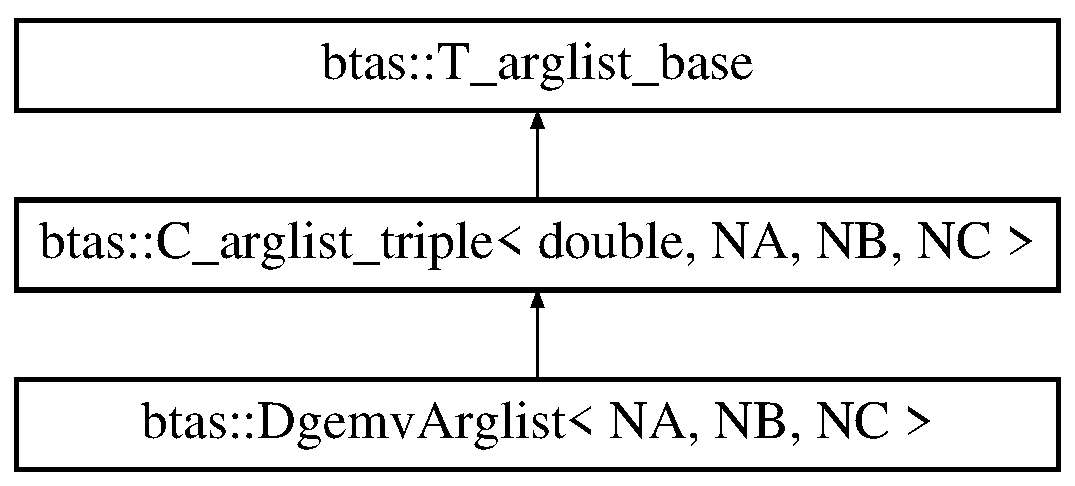
\includegraphics[height=3.000000cm]{df/d7c/classbtas_1_1DgemvArglist}
\end{center}
\end{figure}
\subsection*{Public Member Functions}
\begin{DoxyCompactItemize}
\item 
{\bf Dgemv\-Arglist} ()
\begin{DoxyCompactList}\small\item\em Default constructor. \end{DoxyCompactList}\item 
{\bf Dgemv\-Arglist} (const shared\-\_\-ptr$<$ {\bf D\-Array}$<$ N\-C $>$$>$ \&c\-\_\-ptr, const {\bf B\-T\-A\-S\-\_\-\-T\-R\-A\-N\-S\-P\-O\-S\-E} \&transa={\bf No\-Trans}, const double \&alpha=1.\-0, const double \&beta=1.\-0)
\begin{DoxyCompactList}\small\item\em Initializer. \end{DoxyCompactList}\item 
void {\bf reset} (const shared\-\_\-ptr$<$ {\bf D\-Array}$<$ N\-C $>$$>$ \&c\-\_\-ptr, const {\bf B\-T\-A\-S\-\_\-\-T\-R\-A\-N\-S\-P\-O\-S\-E} \&transa={\bf No\-Trans}, const double \&alpha=1.\-0, const double \&beta=1.\-0)
\begin{DoxyCompactList}\small\item\em Reset arglist. \end{DoxyCompactList}\item 
void {\bf clear} ()
\begin{DoxyCompactList}\small\item\em Clear argments. \end{DoxyCompactList}\item 
void {\bf add} (const shared\-\_\-ptr$<$ {\bf D\-Array}$<$ N\-A $>$$>$ \&a\-\_\-ptr, const shared\-\_\-ptr$<$ {\bf D\-Array}$<$ N\-B $>$$>$ \&b\-\_\-ptr, double scale=1.\-0)
\begin{DoxyCompactList}\small\item\em Add arglist. \end{DoxyCompactList}\item 
void {\bf call} () const 
\begin{DoxyCompactList}\small\item\em Call Dgemv. \end{DoxyCompactList}\end{DoxyCompactItemize}
\subsection*{Private Member Functions}
\begin{DoxyCompactItemize}
\item 
size\-\_\-t {\bf mf\-\_\-flops\-\_\-count} (const shared\-\_\-ptr$<$ {\bf D\-Array}$<$ N\-A $>$$>$ \&a\-\_\-ptr, const shared\-\_\-ptr$<$ {\bf D\-Array}$<$ N\-B $>$$>$ \&b\-\_\-ptr)
\begin{DoxyCompactList}\small\item\em return F\-L\-O\-P\-S count \end{DoxyCompactList}\end{DoxyCompactItemize}
\subsection*{Private Attributes}
\begin{DoxyCompactItemize}
\item 
std\-::vector$<$ double $>$ {\bf m\-\_\-scale}
\begin{DoxyCompactList}\small\item\em this contains index-\/dependent scaling s.\-t. parity, Clebsch-\/\-Gordan coeff., etc. \end{DoxyCompactList}\item 
{\bf B\-T\-A\-S\-\_\-\-T\-R\-A\-N\-S\-P\-O\-S\-E} {\bf m\-\_\-transa}
\item 
double {\bf m\-\_\-alpha}
\item 
double {\bf m\-\_\-beta}
\end{DoxyCompactItemize}
\subsection*{Additional Inherited Members}


\subsection{Detailed Description}
\subsubsection*{template$<$size\-\_\-t N\-A, size\-\_\-t N\-B, size\-\_\-t N\-C$>$class btas\-::\-Dgemv\-Arglist$<$ N\-A, N\-B, N\-C $>$}



Definition at line 118 of file Darglist.\-h.



\subsection{Constructor \& Destructor Documentation}
\index{btas\-::\-Dgemv\-Arglist@{btas\-::\-Dgemv\-Arglist}!Dgemv\-Arglist@{Dgemv\-Arglist}}
\index{Dgemv\-Arglist@{Dgemv\-Arglist}!btas::DgemvArglist@{btas\-::\-Dgemv\-Arglist}}
\subsubsection[{Dgemv\-Arglist}]{\setlength{\rightskip}{0pt plus 5cm}template$<$size\-\_\-t N\-A, size\-\_\-t N\-B, size\-\_\-t N\-C$>$ {\bf btas\-::\-Dgemv\-Arglist}$<$ N\-A, N\-B, N\-C $>$\-::{\bf Dgemv\-Arglist} (
\begin{DoxyParamCaption}
{}
\end{DoxyParamCaption}
)\hspace{0.3cm}{\ttfamily [inline]}}\label{df/d7c/classbtas_1_1DgemvArglist_a746e07e932c54c32cdcd6d8aa78b8e3a}


Default constructor. 



Definition at line 135 of file Darglist.\-h.

\index{btas\-::\-Dgemv\-Arglist@{btas\-::\-Dgemv\-Arglist}!Dgemv\-Arglist@{Dgemv\-Arglist}}
\index{Dgemv\-Arglist@{Dgemv\-Arglist}!btas::DgemvArglist@{btas\-::\-Dgemv\-Arglist}}
\subsubsection[{Dgemv\-Arglist}]{\setlength{\rightskip}{0pt plus 5cm}template$<$size\-\_\-t N\-A, size\-\_\-t N\-B, size\-\_\-t N\-C$>$ {\bf btas\-::\-Dgemv\-Arglist}$<$ N\-A, N\-B, N\-C $>$\-::{\bf Dgemv\-Arglist} (
\begin{DoxyParamCaption}
\item[{const shared\-\_\-ptr$<$ {\bf D\-Array}$<$ N\-C $>$$>$ \&}]{c\-\_\-ptr, }
\item[{const {\bf B\-T\-A\-S\-\_\-\-T\-R\-A\-N\-S\-P\-O\-S\-E} \&}]{transa = {\ttfamily {\bf No\-Trans}}, }
\item[{const double \&}]{alpha = {\ttfamily 1.0}, }
\item[{const double \&}]{beta = {\ttfamily 1.0}}
\end{DoxyParamCaption}
)\hspace{0.3cm}{\ttfamily [inline]}}\label{df/d7c/classbtas_1_1DgemvArglist_a098247ab2c2d55618cb09b7b01ed98db}


Initializer. 



Definition at line 138 of file Darglist.\-h.



\subsection{Member Function Documentation}
\index{btas\-::\-Dgemv\-Arglist@{btas\-::\-Dgemv\-Arglist}!add@{add}}
\index{add@{add}!btas::DgemvArglist@{btas\-::\-Dgemv\-Arglist}}
\subsubsection[{add}]{\setlength{\rightskip}{0pt plus 5cm}template$<$size\-\_\-t N\-A, size\-\_\-t N\-B, size\-\_\-t N\-C$>$ void {\bf btas\-::\-Dgemv\-Arglist}$<$ N\-A, N\-B, N\-C $>$\-::add (
\begin{DoxyParamCaption}
\item[{const shared\-\_\-ptr$<$ {\bf D\-Array}$<$ N\-A $>$$>$ \&}]{a\-\_\-ptr, }
\item[{const shared\-\_\-ptr$<$ {\bf D\-Array}$<$ N\-B $>$$>$ \&}]{b\-\_\-ptr, }
\item[{double}]{scale = {\ttfamily 1.0}}
\end{DoxyParamCaption}
)\hspace{0.3cm}{\ttfamily [inline]}}\label{df/d7c/classbtas_1_1DgemvArglist_a87fed56f5fba8c029e69a9e8c209ffb7}


Add arglist. 



Definition at line 165 of file Darglist.\-h.



References btas\-::\-C\-\_\-arglist\-\_\-triple$<$ T, N1, N2, N3 $>$\-::add(), and btas\-::\-Dgemv\-Arglist$<$ N\-A, N\-B, N\-C $>$\-::m\-\_\-scale.



Referenced by btas\-::thread\-\_\-\-S\-Dgemv().

\index{btas\-::\-Dgemv\-Arglist@{btas\-::\-Dgemv\-Arglist}!call@{call}}
\index{call@{call}!btas::DgemvArglist@{btas\-::\-Dgemv\-Arglist}}
\subsubsection[{call}]{\setlength{\rightskip}{0pt plus 5cm}template$<$size\-\_\-t N\-A, size\-\_\-t N\-B, size\-\_\-t N\-C$>$ void {\bf btas\-::\-Dgemv\-Arglist}$<$ N\-A, N\-B, N\-C $>$\-::call (
\begin{DoxyParamCaption}
{}
\end{DoxyParamCaption}
) const\hspace{0.3cm}{\ttfamily [inline]}}\label{df/d7c/classbtas_1_1DgemvArglist_aec28f781b0e5f289b99c5832d627c817}


Call Dgemv. 



Definition at line 171 of file Darglist.\-h.



References btas\-::\-Dgemv(), btas\-::\-Dgemv\-Arglist$<$ N\-A, N\-B, N\-C $>$\-::m\-\_\-alpha, btas\-::\-Dgemv\-Arglist$<$ N\-A, N\-B, N\-C $>$\-::m\-\_\-beta, btas\-::\-Dgemv\-Arglist$<$ N\-A, N\-B, N\-C $>$\-::m\-\_\-scale, btas\-::\-Dgemv\-Arglist$<$ N\-A, N\-B, N\-C $>$\-::m\-\_\-transa, and btas\-::\-C\-\_\-arglist\-\_\-triple$<$ double, N\-A, N\-B, N\-C $>$\-::size().

\index{btas\-::\-Dgemv\-Arglist@{btas\-::\-Dgemv\-Arglist}!clear@{clear}}
\index{clear@{clear}!btas::DgemvArglist@{btas\-::\-Dgemv\-Arglist}}
\subsubsection[{clear}]{\setlength{\rightskip}{0pt plus 5cm}template$<$size\-\_\-t N\-A, size\-\_\-t N\-B, size\-\_\-t N\-C$>$ void {\bf btas\-::\-Dgemv\-Arglist}$<$ N\-A, N\-B, N\-C $>$\-::clear (
\begin{DoxyParamCaption}
{}
\end{DoxyParamCaption}
)\hspace{0.3cm}{\ttfamily [inline]}, {\ttfamily [virtual]}}\label{df/d7c/classbtas_1_1DgemvArglist_a48b444eefcb720024388a39ce05a7b3a}


Clear argments. 



Reimplemented from {\bf btas\-::\-C\-\_\-arglist\-\_\-triple$<$ double, N\-A, N\-B, N\-C $>$} \doxyref{}{p.}{d5/d67/classbtas_1_1C__arglist__triple_a2df507deb003fe1a16a692dd76a408c5}.



Definition at line 156 of file Darglist.\-h.



References btas\-::\-C\-\_\-arglist\-\_\-triple$<$ T, N1, N2, N3 $>$\-::clear(), btas\-::\-Dgemv\-Arglist$<$ N\-A, N\-B, N\-C $>$\-::m\-\_\-alpha, btas\-::\-Dgemv\-Arglist$<$ N\-A, N\-B, N\-C $>$\-::m\-\_\-beta, btas\-::\-Dgemv\-Arglist$<$ N\-A, N\-B, N\-C $>$\-::m\-\_\-scale, btas\-::\-Dgemv\-Arglist$<$ N\-A, N\-B, N\-C $>$\-::m\-\_\-transa, and btas\-::\-No\-Trans.

\index{btas\-::\-Dgemv\-Arglist@{btas\-::\-Dgemv\-Arglist}!mf\-\_\-flops\-\_\-count@{mf\-\_\-flops\-\_\-count}}
\index{mf\-\_\-flops\-\_\-count@{mf\-\_\-flops\-\_\-count}!btas::DgemvArglist@{btas\-::\-Dgemv\-Arglist}}
\subsubsection[{mf\-\_\-flops\-\_\-count}]{\setlength{\rightskip}{0pt plus 5cm}template$<$size\-\_\-t N\-A, size\-\_\-t N\-B, size\-\_\-t N\-C$>$ size\-\_\-t {\bf btas\-::\-Dgemv\-Arglist}$<$ N\-A, N\-B, N\-C $>$\-::mf\-\_\-flops\-\_\-count (
\begin{DoxyParamCaption}
\item[{const shared\-\_\-ptr$<$ {\bf D\-Array}$<$ N\-A $>$$>$ \&}]{a\-\_\-ptr, }
\item[{const shared\-\_\-ptr$<$ {\bf D\-Array}$<$ N\-B $>$$>$ \&}]{b\-\_\-ptr}
\end{DoxyParamCaption}
)\hspace{0.3cm}{\ttfamily [inline]}, {\ttfamily [private]}}\label{df/d7c/classbtas_1_1DgemvArglist_af1de71ea2e50335062b108b2d3d2bcea}


return F\-L\-O\-P\-S count 



Definition at line 131 of file Darglist.\-h.

\index{btas\-::\-Dgemv\-Arglist@{btas\-::\-Dgemv\-Arglist}!reset@{reset}}
\index{reset@{reset}!btas::DgemvArglist@{btas\-::\-Dgemv\-Arglist}}
\subsubsection[{reset}]{\setlength{\rightskip}{0pt plus 5cm}template$<$size\-\_\-t N\-A, size\-\_\-t N\-B, size\-\_\-t N\-C$>$ void {\bf btas\-::\-Dgemv\-Arglist}$<$ N\-A, N\-B, N\-C $>$\-::reset (
\begin{DoxyParamCaption}
\item[{const shared\-\_\-ptr$<$ {\bf D\-Array}$<$ N\-C $>$$>$ \&}]{c\-\_\-ptr, }
\item[{const {\bf B\-T\-A\-S\-\_\-\-T\-R\-A\-N\-S\-P\-O\-S\-E} \&}]{transa = {\ttfamily {\bf No\-Trans}}, }
\item[{const double \&}]{alpha = {\ttfamily 1.0}, }
\item[{const double \&}]{beta = {\ttfamily 1.0}}
\end{DoxyParamCaption}
)\hspace{0.3cm}{\ttfamily [inline]}}\label{df/d7c/classbtas_1_1DgemvArglist_a465ee75bd9018a8e22faab003b7396bd}


Reset arglist. 



Definition at line 146 of file Darglist.\-h.



References btas\-::\-Dgemv\-Arglist$<$ N\-A, N\-B, N\-C $>$\-::m\-\_\-alpha, btas\-::\-Dgemv\-Arglist$<$ N\-A, N\-B, N\-C $>$\-::m\-\_\-beta, btas\-::\-Dgemv\-Arglist$<$ N\-A, N\-B, N\-C $>$\-::m\-\_\-transa, and btas\-::\-C\-\_\-arglist\-\_\-triple$<$ T, N1, N2, N3 $>$\-::reset().



Referenced by btas\-::thread\-\_\-\-S\-Dgemv().



\subsection{Field Documentation}
\index{btas\-::\-Dgemv\-Arglist@{btas\-::\-Dgemv\-Arglist}!m\-\_\-alpha@{m\-\_\-alpha}}
\index{m\-\_\-alpha@{m\-\_\-alpha}!btas::DgemvArglist@{btas\-::\-Dgemv\-Arglist}}
\subsubsection[{m\-\_\-alpha}]{\setlength{\rightskip}{0pt plus 5cm}template$<$size\-\_\-t N\-A, size\-\_\-t N\-B, size\-\_\-t N\-C$>$ double {\bf btas\-::\-Dgemv\-Arglist}$<$ N\-A, N\-B, N\-C $>$\-::m\-\_\-alpha\hspace{0.3cm}{\ttfamily [private]}}\label{df/d7c/classbtas_1_1DgemvArglist_a22f23d1edcc10908e13a8880779a467b}


Definition at line 126 of file Darglist.\-h.



Referenced by btas\-::\-Dgemv\-Arglist$<$ N\-A, N\-B, N\-C $>$\-::call(), btas\-::\-Dgemv\-Arglist$<$ N\-A, N\-B, N\-C $>$\-::clear(), and btas\-::\-Dgemv\-Arglist$<$ N\-A, N\-B, N\-C $>$\-::reset().

\index{btas\-::\-Dgemv\-Arglist@{btas\-::\-Dgemv\-Arglist}!m\-\_\-beta@{m\-\_\-beta}}
\index{m\-\_\-beta@{m\-\_\-beta}!btas::DgemvArglist@{btas\-::\-Dgemv\-Arglist}}
\subsubsection[{m\-\_\-beta}]{\setlength{\rightskip}{0pt plus 5cm}template$<$size\-\_\-t N\-A, size\-\_\-t N\-B, size\-\_\-t N\-C$>$ double {\bf btas\-::\-Dgemv\-Arglist}$<$ N\-A, N\-B, N\-C $>$\-::m\-\_\-beta\hspace{0.3cm}{\ttfamily [private]}}\label{df/d7c/classbtas_1_1DgemvArglist_a557620a84dc653458444f3d21275c5da}


Definition at line 128 of file Darglist.\-h.



Referenced by btas\-::\-Dgemv\-Arglist$<$ N\-A, N\-B, N\-C $>$\-::call(), btas\-::\-Dgemv\-Arglist$<$ N\-A, N\-B, N\-C $>$\-::clear(), and btas\-::\-Dgemv\-Arglist$<$ N\-A, N\-B, N\-C $>$\-::reset().

\index{btas\-::\-Dgemv\-Arglist@{btas\-::\-Dgemv\-Arglist}!m\-\_\-scale@{m\-\_\-scale}}
\index{m\-\_\-scale@{m\-\_\-scale}!btas::DgemvArglist@{btas\-::\-Dgemv\-Arglist}}
\subsubsection[{m\-\_\-scale}]{\setlength{\rightskip}{0pt plus 5cm}template$<$size\-\_\-t N\-A, size\-\_\-t N\-B, size\-\_\-t N\-C$>$ std\-::vector$<$double$>$ {\bf btas\-::\-Dgemv\-Arglist}$<$ N\-A, N\-B, N\-C $>$\-::m\-\_\-scale\hspace{0.3cm}{\ttfamily [private]}}\label{df/d7c/classbtas_1_1DgemvArglist_a45742fa341757c722f4bb0db557ff201}


this contains index-\/dependent scaling s.\-t. parity, Clebsch-\/\-Gordan coeff., etc. 



Definition at line 122 of file Darglist.\-h.



Referenced by btas\-::\-Dgemv\-Arglist$<$ N\-A, N\-B, N\-C $>$\-::add(), btas\-::\-Dgemv\-Arglist$<$ N\-A, N\-B, N\-C $>$\-::call(), and btas\-::\-Dgemv\-Arglist$<$ N\-A, N\-B, N\-C $>$\-::clear().

\index{btas\-::\-Dgemv\-Arglist@{btas\-::\-Dgemv\-Arglist}!m\-\_\-transa@{m\-\_\-transa}}
\index{m\-\_\-transa@{m\-\_\-transa}!btas::DgemvArglist@{btas\-::\-Dgemv\-Arglist}}
\subsubsection[{m\-\_\-transa}]{\setlength{\rightskip}{0pt plus 5cm}template$<$size\-\_\-t N\-A, size\-\_\-t N\-B, size\-\_\-t N\-C$>$ {\bf B\-T\-A\-S\-\_\-\-T\-R\-A\-N\-S\-P\-O\-S\-E} {\bf btas\-::\-Dgemv\-Arglist}$<$ N\-A, N\-B, N\-C $>$\-::m\-\_\-transa\hspace{0.3cm}{\ttfamily [private]}}\label{df/d7c/classbtas_1_1DgemvArglist_a31778123e489903a2482fc0a939c3e4d}


Definition at line 124 of file Darglist.\-h.



Referenced by btas\-::\-Dgemv\-Arglist$<$ N\-A, N\-B, N\-C $>$\-::call(), btas\-::\-Dgemv\-Arglist$<$ N\-A, N\-B, N\-C $>$\-::clear(), and btas\-::\-Dgemv\-Arglist$<$ N\-A, N\-B, N\-C $>$\-::reset().



The documentation for this class was generated from the following file\-:\begin{DoxyCompactItemize}
\item 
include/btas/\-D\-E\-N\-S\-E/{\bf Darglist.\-h}\end{DoxyCompactItemize}

\section{btas\-:\-:Dger\-Arglist$<$ N\-A, N\-B, N\-C $>$ Class Template Reference}
\label{da/db6/classbtas_1_1DgerArglist}\index{btas\-::\-Dger\-Arglist$<$ N\-A, N\-B, N\-C $>$@{btas\-::\-Dger\-Arglist$<$ N\-A, N\-B, N\-C $>$}}


{\ttfamily \#include $<$Darglist.\-h$>$}

Inheritance diagram for btas\-:\-:Dger\-Arglist$<$ N\-A, N\-B, N\-C $>$\-:\begin{figure}[H]
\begin{center}
\leavevmode
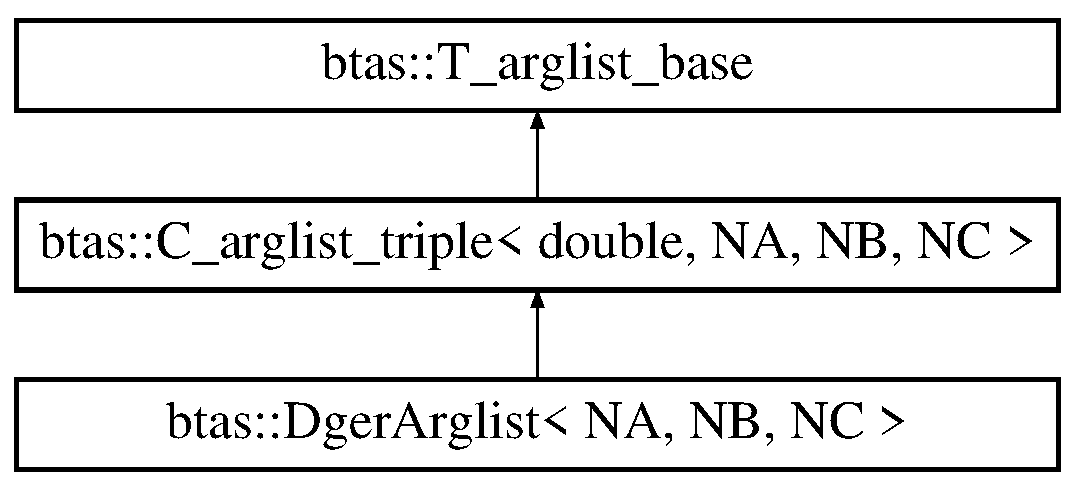
\includegraphics[height=3.000000cm]{da/db6/classbtas_1_1DgerArglist}
\end{center}
\end{figure}
\subsection*{Public Member Functions}
\begin{DoxyCompactItemize}
\item 
{\bf Dger\-Arglist} ()
\begin{DoxyCompactList}\small\item\em Default constructor. \end{DoxyCompactList}\item 
{\bf Dger\-Arglist} (const shared\-\_\-ptr$<$ {\bf D\-Array}$<$ N\-C $>$$>$ \&c\-\_\-ptr, const double \&alpha=1.\-0)
\item 
void {\bf reset} (const shared\-\_\-ptr$<$ {\bf D\-Array}$<$ N\-C $>$$>$ \&c\-\_\-ptr, const double \&alpha=1.\-0)
\begin{DoxyCompactList}\small\item\em Reset arglist. \end{DoxyCompactList}\item 
void {\bf clear} ()
\begin{DoxyCompactList}\small\item\em Clear argments. \end{DoxyCompactList}\item 
void {\bf add} (const shared\-\_\-ptr$<$ {\bf D\-Array}$<$ N\-A $>$$>$ \&a\-\_\-ptr, const shared\-\_\-ptr$<$ {\bf D\-Array}$<$ N\-B $>$$>$ \&b\-\_\-ptr, double scale=1.\-0)
\begin{DoxyCompactList}\small\item\em Add arglist. \end{DoxyCompactList}\item 
void {\bf call} () const 
\begin{DoxyCompactList}\small\item\em Call Dger. \end{DoxyCompactList}\end{DoxyCompactItemize}
\subsection*{Private Member Functions}
\begin{DoxyCompactItemize}
\item 
size\-\_\-t {\bf mf\-\_\-flops\-\_\-count} (const shared\-\_\-ptr$<$ {\bf D\-Array}$<$ N\-A $>$$>$ \&a\-\_\-ptr, const shared\-\_\-ptr$<$ {\bf D\-Array}$<$ N\-B $>$$>$ \&b\-\_\-ptr)
\begin{DoxyCompactList}\small\item\em return F\-L\-O\-P\-S count \end{DoxyCompactList}\end{DoxyCompactItemize}
\subsection*{Private Attributes}
\begin{DoxyCompactItemize}
\item 
std\-::vector$<$ double $>$ {\bf m\-\_\-scale}
\begin{DoxyCompactList}\small\item\em this contains index-\/dependent scaling s.\-t. parity, Clebsch-\/\-Gordan coeff., etc. \end{DoxyCompactList}\item 
double {\bf m\-\_\-alpha}
\end{DoxyCompactItemize}
\subsection*{Additional Inherited Members}


\subsection{Detailed Description}
\subsubsection*{template$<$size\-\_\-t N\-A, size\-\_\-t N\-B, size\-\_\-t N\-C$>$class btas\-::\-Dger\-Arglist$<$ N\-A, N\-B, N\-C $>$}



Definition at line 181 of file Darglist.\-h.



\subsection{Constructor \& Destructor Documentation}
\index{btas\-::\-Dger\-Arglist@{btas\-::\-Dger\-Arglist}!Dger\-Arglist@{Dger\-Arglist}}
\index{Dger\-Arglist@{Dger\-Arglist}!btas::DgerArglist@{btas\-::\-Dger\-Arglist}}
\subsubsection[{Dger\-Arglist}]{\setlength{\rightskip}{0pt plus 5cm}template$<$size\-\_\-t N\-A, size\-\_\-t N\-B, size\-\_\-t N\-C$>$ {\bf btas\-::\-Dger\-Arglist}$<$ N\-A, N\-B, N\-C $>$\-::{\bf Dger\-Arglist} (
\begin{DoxyParamCaption}
{}
\end{DoxyParamCaption}
)\hspace{0.3cm}{\ttfamily [inline]}}\label{da/db6/classbtas_1_1DgerArglist_a5c0dcf17c4c15d87c280830435d34920}


Default constructor. 



Definition at line 194 of file Darglist.\-h.

\index{btas\-::\-Dger\-Arglist@{btas\-::\-Dger\-Arglist}!Dger\-Arglist@{Dger\-Arglist}}
\index{Dger\-Arglist@{Dger\-Arglist}!btas::DgerArglist@{btas\-::\-Dger\-Arglist}}
\subsubsection[{Dger\-Arglist}]{\setlength{\rightskip}{0pt plus 5cm}template$<$size\-\_\-t N\-A, size\-\_\-t N\-B, size\-\_\-t N\-C$>$ {\bf btas\-::\-Dger\-Arglist}$<$ N\-A, N\-B, N\-C $>$\-::{\bf Dger\-Arglist} (
\begin{DoxyParamCaption}
\item[{const shared\-\_\-ptr$<$ {\bf D\-Array}$<$ N\-C $>$$>$ \&}]{c\-\_\-ptr, }
\item[{const double \&}]{alpha = {\ttfamily 1.0}}
\end{DoxyParamCaption}
)\hspace{0.3cm}{\ttfamily [inline]}}\label{da/db6/classbtas_1_1DgerArglist_adf0896b31c82eadfd9e1424a36c9d2e2}


Definition at line 196 of file Darglist.\-h.



\subsection{Member Function Documentation}
\index{btas\-::\-Dger\-Arglist@{btas\-::\-Dger\-Arglist}!add@{add}}
\index{add@{add}!btas::DgerArglist@{btas\-::\-Dger\-Arglist}}
\subsubsection[{add}]{\setlength{\rightskip}{0pt plus 5cm}template$<$size\-\_\-t N\-A, size\-\_\-t N\-B, size\-\_\-t N\-C$>$ void {\bf btas\-::\-Dger\-Arglist}$<$ N\-A, N\-B, N\-C $>$\-::add (
\begin{DoxyParamCaption}
\item[{const shared\-\_\-ptr$<$ {\bf D\-Array}$<$ N\-A $>$$>$ \&}]{a\-\_\-ptr, }
\item[{const shared\-\_\-ptr$<$ {\bf D\-Array}$<$ N\-B $>$$>$ \&}]{b\-\_\-ptr, }
\item[{double}]{scale = {\ttfamily 1.0}}
\end{DoxyParamCaption}
)\hspace{0.3cm}{\ttfamily [inline]}}\label{da/db6/classbtas_1_1DgerArglist_a1cc61d98f06df930dc79f7e043f5cbab}


Add arglist. 



Definition at line 215 of file Darglist.\-h.



References btas\-::\-C\-\_\-arglist\-\_\-triple$<$ T, N1, N2, N3 $>$\-::add(), and btas\-::\-Dger\-Arglist$<$ N\-A, N\-B, N\-C $>$\-::m\-\_\-scale.



Referenced by btas\-::thread\-\_\-\-S\-Dger().

\index{btas\-::\-Dger\-Arglist@{btas\-::\-Dger\-Arglist}!call@{call}}
\index{call@{call}!btas::DgerArglist@{btas\-::\-Dger\-Arglist}}
\subsubsection[{call}]{\setlength{\rightskip}{0pt plus 5cm}template$<$size\-\_\-t N\-A, size\-\_\-t N\-B, size\-\_\-t N\-C$>$ void {\bf btas\-::\-Dger\-Arglist}$<$ N\-A, N\-B, N\-C $>$\-::call (
\begin{DoxyParamCaption}
{}
\end{DoxyParamCaption}
) const\hspace{0.3cm}{\ttfamily [inline]}}\label{da/db6/classbtas_1_1DgerArglist_a573486de45c5dc8ea3838c7cad1ed0db}


Call Dger. 



Definition at line 221 of file Darglist.\-h.



References btas\-::\-Dger(), btas\-::\-Dger\-Arglist$<$ N\-A, N\-B, N\-C $>$\-::m\-\_\-alpha, btas\-::\-Dger\-Arglist$<$ N\-A, N\-B, N\-C $>$\-::m\-\_\-scale, and btas\-::\-C\-\_\-arglist\-\_\-triple$<$ double, N\-A, N\-B, N\-C $>$\-::size().

\index{btas\-::\-Dger\-Arglist@{btas\-::\-Dger\-Arglist}!clear@{clear}}
\index{clear@{clear}!btas::DgerArglist@{btas\-::\-Dger\-Arglist}}
\subsubsection[{clear}]{\setlength{\rightskip}{0pt plus 5cm}template$<$size\-\_\-t N\-A, size\-\_\-t N\-B, size\-\_\-t N\-C$>$ void {\bf btas\-::\-Dger\-Arglist}$<$ N\-A, N\-B, N\-C $>$\-::clear (
\begin{DoxyParamCaption}
{}
\end{DoxyParamCaption}
)\hspace{0.3cm}{\ttfamily [inline]}, {\ttfamily [virtual]}}\label{da/db6/classbtas_1_1DgerArglist_a43a8a8922741041d0724da534ccf866b}


Clear argments. 



Reimplemented from {\bf btas\-::\-C\-\_\-arglist\-\_\-triple$<$ double, N\-A, N\-B, N\-C $>$} \doxyref{}{p.}{d5/d67/classbtas_1_1C__arglist__triple_a2df507deb003fe1a16a692dd76a408c5}.



Definition at line 208 of file Darglist.\-h.



References btas\-::\-C\-\_\-arglist\-\_\-triple$<$ T, N1, N2, N3 $>$\-::clear(), btas\-::\-Dger\-Arglist$<$ N\-A, N\-B, N\-C $>$\-::m\-\_\-alpha, and btas\-::\-Dger\-Arglist$<$ N\-A, N\-B, N\-C $>$\-::m\-\_\-scale.

\index{btas\-::\-Dger\-Arglist@{btas\-::\-Dger\-Arglist}!mf\-\_\-flops\-\_\-count@{mf\-\_\-flops\-\_\-count}}
\index{mf\-\_\-flops\-\_\-count@{mf\-\_\-flops\-\_\-count}!btas::DgerArglist@{btas\-::\-Dger\-Arglist}}
\subsubsection[{mf\-\_\-flops\-\_\-count}]{\setlength{\rightskip}{0pt plus 5cm}template$<$size\-\_\-t N\-A, size\-\_\-t N\-B, size\-\_\-t N\-C$>$ size\-\_\-t {\bf btas\-::\-Dger\-Arglist}$<$ N\-A, N\-B, N\-C $>$\-::mf\-\_\-flops\-\_\-count (
\begin{DoxyParamCaption}
\item[{const shared\-\_\-ptr$<$ {\bf D\-Array}$<$ N\-A $>$$>$ \&}]{a\-\_\-ptr, }
\item[{const shared\-\_\-ptr$<$ {\bf D\-Array}$<$ N\-B $>$$>$ \&}]{b\-\_\-ptr}
\end{DoxyParamCaption}
)\hspace{0.3cm}{\ttfamily [inline]}, {\ttfamily [private]}}\label{da/db6/classbtas_1_1DgerArglist_ae091d8dfeb314e46973ef86a888395d2}


return F\-L\-O\-P\-S count 



Definition at line 190 of file Darglist.\-h.

\index{btas\-::\-Dger\-Arglist@{btas\-::\-Dger\-Arglist}!reset@{reset}}
\index{reset@{reset}!btas::DgerArglist@{btas\-::\-Dger\-Arglist}}
\subsubsection[{reset}]{\setlength{\rightskip}{0pt plus 5cm}template$<$size\-\_\-t N\-A, size\-\_\-t N\-B, size\-\_\-t N\-C$>$ void {\bf btas\-::\-Dger\-Arglist}$<$ N\-A, N\-B, N\-C $>$\-::reset (
\begin{DoxyParamCaption}
\item[{const shared\-\_\-ptr$<$ {\bf D\-Array}$<$ N\-C $>$$>$ \&}]{c\-\_\-ptr, }
\item[{const double \&}]{alpha = {\ttfamily 1.0}}
\end{DoxyParamCaption}
)\hspace{0.3cm}{\ttfamily [inline]}}\label{da/db6/classbtas_1_1DgerArglist_a4d193365ea8979e1913911e8ffa2c981}


Reset arglist. 



Definition at line 202 of file Darglist.\-h.



References btas\-::\-Dger\-Arglist$<$ N\-A, N\-B, N\-C $>$\-::m\-\_\-alpha, and btas\-::\-C\-\_\-arglist\-\_\-triple$<$ T, N1, N2, N3 $>$\-::reset().



\subsection{Field Documentation}
\index{btas\-::\-Dger\-Arglist@{btas\-::\-Dger\-Arglist}!m\-\_\-alpha@{m\-\_\-alpha}}
\index{m\-\_\-alpha@{m\-\_\-alpha}!btas::DgerArglist@{btas\-::\-Dger\-Arglist}}
\subsubsection[{m\-\_\-alpha}]{\setlength{\rightskip}{0pt plus 5cm}template$<$size\-\_\-t N\-A, size\-\_\-t N\-B, size\-\_\-t N\-C$>$ double {\bf btas\-::\-Dger\-Arglist}$<$ N\-A, N\-B, N\-C $>$\-::m\-\_\-alpha\hspace{0.3cm}{\ttfamily [private]}}\label{da/db6/classbtas_1_1DgerArglist_a0d3533782348de6543dfe780d7db0e71}


Definition at line 187 of file Darglist.\-h.



Referenced by btas\-::\-Dger\-Arglist$<$ N\-A, N\-B, N\-C $>$\-::call(), btas\-::\-Dger\-Arglist$<$ N\-A, N\-B, N\-C $>$\-::clear(), and btas\-::\-Dger\-Arglist$<$ N\-A, N\-B, N\-C $>$\-::reset().

\index{btas\-::\-Dger\-Arglist@{btas\-::\-Dger\-Arglist}!m\-\_\-scale@{m\-\_\-scale}}
\index{m\-\_\-scale@{m\-\_\-scale}!btas::DgerArglist@{btas\-::\-Dger\-Arglist}}
\subsubsection[{m\-\_\-scale}]{\setlength{\rightskip}{0pt plus 5cm}template$<$size\-\_\-t N\-A, size\-\_\-t N\-B, size\-\_\-t N\-C$>$ std\-::vector$<$double$>$ {\bf btas\-::\-Dger\-Arglist}$<$ N\-A, N\-B, N\-C $>$\-::m\-\_\-scale\hspace{0.3cm}{\ttfamily [private]}}\label{da/db6/classbtas_1_1DgerArglist_adfcfebc0f11af221edf44ba980628ee1}


this contains index-\/dependent scaling s.\-t. parity, Clebsch-\/\-Gordan coeff., etc. 



Definition at line 185 of file Darglist.\-h.



Referenced by btas\-::\-Dger\-Arglist$<$ N\-A, N\-B, N\-C $>$\-::add(), btas\-::\-Dger\-Arglist$<$ N\-A, N\-B, N\-C $>$\-::call(), and btas\-::\-Dger\-Arglist$<$ N\-A, N\-B, N\-C $>$\-::clear().



The documentation for this class was generated from the following file\-:\begin{DoxyCompactItemize}
\item 
include/btas/\-D\-E\-N\-S\-E/{\bf Darglist.\-h}\end{DoxyCompactItemize}

\section{btas\-:\-:Dgesvd\-Arglist$<$ N\-A, N\-U $>$ Class Template Reference}
\label{d5/d3c/classbtas_1_1DgesvdArglist}\index{btas\-::\-Dgesvd\-Arglist$<$ N\-A, N\-U $>$@{btas\-::\-Dgesvd\-Arglist$<$ N\-A, N\-U $>$}}


{\ttfamily \#include $<$Darglist.\-h$>$}

Inheritance diagram for btas\-:\-:Dgesvd\-Arglist$<$ N\-A, N\-U $>$\-:\begin{figure}[H]
\begin{center}
\leavevmode
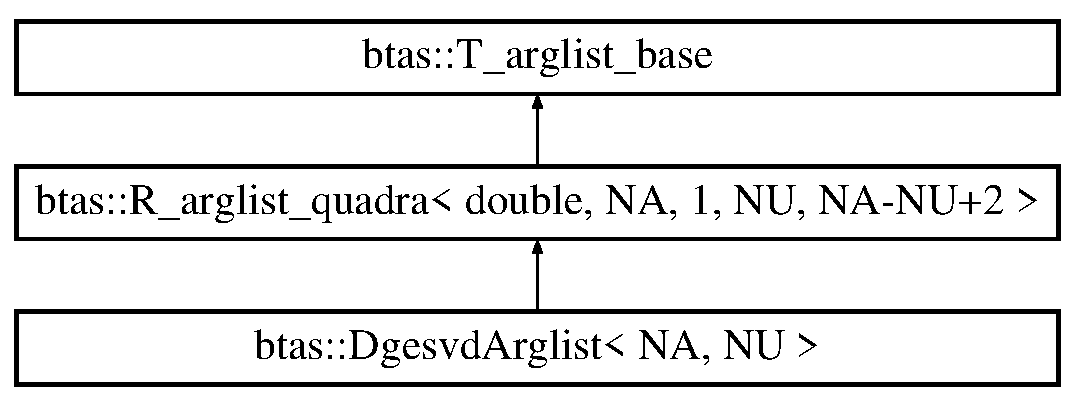
\includegraphics[height=3.000000cm]{d5/d3c/classbtas_1_1DgesvdArglist}
\end{center}
\end{figure}
\subsection*{Public Member Functions}
\begin{DoxyCompactItemize}
\item 
{\bf Dgesvd\-Arglist} ()
\begin{DoxyCompactList}\small\item\em Default constructor. \end{DoxyCompactList}\item 
{\bf Dgesvd\-Arglist} (const shared\-\_\-ptr$<$ {\bf D\-Array}$<$ N\-A $>$ $>$ \&a\-\_\-ptr, const shared\-\_\-ptr$<$ {\bf D\-Array}$<$ 1 $>$ $>$ \&s\-\_\-ptr, const shared\-\_\-ptr$<$ {\bf D\-Array}$<$ N\-U $>$ $>$ \&u\-\_\-ptr, const shared\-\_\-ptr$<$ {\bf D\-Array}$<$ N\-A-\/N\-U+2 $>$$>$ \&v\-\_\-ptr, bool calc\-\_\-u=false, bool calc\-\_\-vt=false)
\begin{DoxyCompactList}\small\item\em Initializer. \end{DoxyCompactList}\item 
void {\bf call} () const 
\begin{DoxyCompactList}\small\item\em Call Dgesvd. \end{DoxyCompactList}\end{DoxyCompactItemize}
\subsection*{Private Attributes}
\begin{DoxyCompactItemize}
\item 
bool {\bf m\-\_\-calc\-\_\-u}
\item 
bool {\bf m\-\_\-calc\-\_\-vt}
\end{DoxyCompactItemize}
\subsection*{Additional Inherited Members}


\subsection{Detailed Description}
\subsubsection*{template$<$size\-\_\-t N\-A, size\-\_\-t N\-U$>$class btas\-::\-Dgesvd\-Arglist$<$ N\-A, N\-U $>$}



Definition at line 314 of file Darglist.\-h.



\subsection{Constructor \& Destructor Documentation}
\index{btas\-::\-Dgesvd\-Arglist@{btas\-::\-Dgesvd\-Arglist}!Dgesvd\-Arglist@{Dgesvd\-Arglist}}
\index{Dgesvd\-Arglist@{Dgesvd\-Arglist}!btas::DgesvdArglist@{btas\-::\-Dgesvd\-Arglist}}
\subsubsection[{Dgesvd\-Arglist}]{\setlength{\rightskip}{0pt plus 5cm}template$<$size\-\_\-t N\-A, size\-\_\-t N\-U$>$ {\bf btas\-::\-Dgesvd\-Arglist}$<$ N\-A, N\-U $>$\-::{\bf Dgesvd\-Arglist} (
\begin{DoxyParamCaption}
{}
\end{DoxyParamCaption}
)\hspace{0.3cm}{\ttfamily [inline]}}\label{d5/d3c/classbtas_1_1DgesvdArglist_a058a32cfe701f4ce0585c812ad6b95b8}


Default constructor. 



Definition at line 320 of file Darglist.\-h.

\index{btas\-::\-Dgesvd\-Arglist@{btas\-::\-Dgesvd\-Arglist}!Dgesvd\-Arglist@{Dgesvd\-Arglist}}
\index{Dgesvd\-Arglist@{Dgesvd\-Arglist}!btas::DgesvdArglist@{btas\-::\-Dgesvd\-Arglist}}
\subsubsection[{Dgesvd\-Arglist}]{\setlength{\rightskip}{0pt plus 5cm}template$<$size\-\_\-t N\-A, size\-\_\-t N\-U$>$ {\bf btas\-::\-Dgesvd\-Arglist}$<$ N\-A, N\-U $>$\-::{\bf Dgesvd\-Arglist} (
\begin{DoxyParamCaption}
\item[{const shared\-\_\-ptr$<$ {\bf D\-Array}$<$ N\-A $>$ $>$ \&}]{a\-\_\-ptr, }
\item[{const shared\-\_\-ptr$<$ {\bf D\-Array}$<$ 1 $>$ $>$ \&}]{s\-\_\-ptr, }
\item[{const shared\-\_\-ptr$<$ {\bf D\-Array}$<$ N\-U $>$ $>$ \&}]{u\-\_\-ptr, }
\item[{const shared\-\_\-ptr$<$ {\bf D\-Array}$<$ N\-A-\/N\-U+2 $>$$>$ \&}]{v\-\_\-ptr, }
\item[{bool}]{calc\-\_\-u = {\ttfamily false}, }
\item[{bool}]{calc\-\_\-vt = {\ttfamily false}}
\end{DoxyParamCaption}
)\hspace{0.3cm}{\ttfamily [inline]}}\label{d5/d3c/classbtas_1_1DgesvdArglist_a6262aa05351fbc38e0ca759f64ac2b00}


Initializer. 



Definition at line 323 of file Darglist.\-h.



\subsection{Member Function Documentation}
\index{btas\-::\-Dgesvd\-Arglist@{btas\-::\-Dgesvd\-Arglist}!call@{call}}
\index{call@{call}!btas::DgesvdArglist@{btas\-::\-Dgesvd\-Arglist}}
\subsubsection[{call}]{\setlength{\rightskip}{0pt plus 5cm}template$<$size\-\_\-t N\-A, size\-\_\-t N\-U$>$ void {\bf btas\-::\-Dgesvd\-Arglist}$<$ N\-A, N\-U $>$\-::call (
\begin{DoxyParamCaption}
{}
\end{DoxyParamCaption}
) const\hspace{0.3cm}{\ttfamily [inline]}}\label{d5/d3c/classbtas_1_1DgesvdArglist_a0e5f1cc0b2d5415086d2d52ec22423fa}


Call Dgesvd. 



Definition at line 329 of file Darglist.\-h.



References btas\-::\-Dgesvd(), btas\-::\-Dgesvd\-Arglist$<$ N\-A, N\-U $>$\-::m\-\_\-calc\-\_\-u, and btas\-::\-Dgesvd\-Arglist$<$ N\-A, N\-U $>$\-::m\-\_\-calc\-\_\-vt.



\subsection{Field Documentation}
\index{btas\-::\-Dgesvd\-Arglist@{btas\-::\-Dgesvd\-Arglist}!m\-\_\-calc\-\_\-u@{m\-\_\-calc\-\_\-u}}
\index{m\-\_\-calc\-\_\-u@{m\-\_\-calc\-\_\-u}!btas::DgesvdArglist@{btas\-::\-Dgesvd\-Arglist}}
\subsubsection[{m\-\_\-calc\-\_\-u}]{\setlength{\rightskip}{0pt plus 5cm}template$<$size\-\_\-t N\-A, size\-\_\-t N\-U$>$ bool {\bf btas\-::\-Dgesvd\-Arglist}$<$ N\-A, N\-U $>$\-::m\-\_\-calc\-\_\-u\hspace{0.3cm}{\ttfamily [private]}}\label{d5/d3c/classbtas_1_1DgesvdArglist_aa9851f71dccca13f0a69255800c9c883}


Definition at line 316 of file Darglist.\-h.



Referenced by btas\-::\-Dgesvd\-Arglist$<$ N\-A, N\-U $>$\-::call().

\index{btas\-::\-Dgesvd\-Arglist@{btas\-::\-Dgesvd\-Arglist}!m\-\_\-calc\-\_\-vt@{m\-\_\-calc\-\_\-vt}}
\index{m\-\_\-calc\-\_\-vt@{m\-\_\-calc\-\_\-vt}!btas::DgesvdArglist@{btas\-::\-Dgesvd\-Arglist}}
\subsubsection[{m\-\_\-calc\-\_\-vt}]{\setlength{\rightskip}{0pt plus 5cm}template$<$size\-\_\-t N\-A, size\-\_\-t N\-U$>$ bool {\bf btas\-::\-Dgesvd\-Arglist}$<$ N\-A, N\-U $>$\-::m\-\_\-calc\-\_\-vt\hspace{0.3cm}{\ttfamily [private]}}\label{d5/d3c/classbtas_1_1DgesvdArglist_aee4abaa95b393b16ab07f4a2e9fedd0e}


Definition at line 317 of file Darglist.\-h.



Referenced by btas\-::\-Dgesvd\-Arglist$<$ N\-A, N\-U $>$\-::call().



The documentation for this class was generated from the following file\-:\begin{DoxyCompactItemize}
\item 
include/btas/\-D\-E\-N\-S\-E/{\bf Darglist.\-h}\end{DoxyCompactItemize}

\section{btas\-:\-:Dpermute\-Arglist$<$ N $>$ Class Template Reference}
\label{d6/d58/classbtas_1_1DpermuteArglist}\index{btas\-::\-Dpermute\-Arglist$<$ N $>$@{btas\-::\-Dpermute\-Arglist$<$ N $>$}}


{\ttfamily \#include $<$Darglist.\-h$>$}

Inheritance diagram for btas\-:\-:Dpermute\-Arglist$<$ N $>$\-:\begin{figure}[H]
\begin{center}
\leavevmode
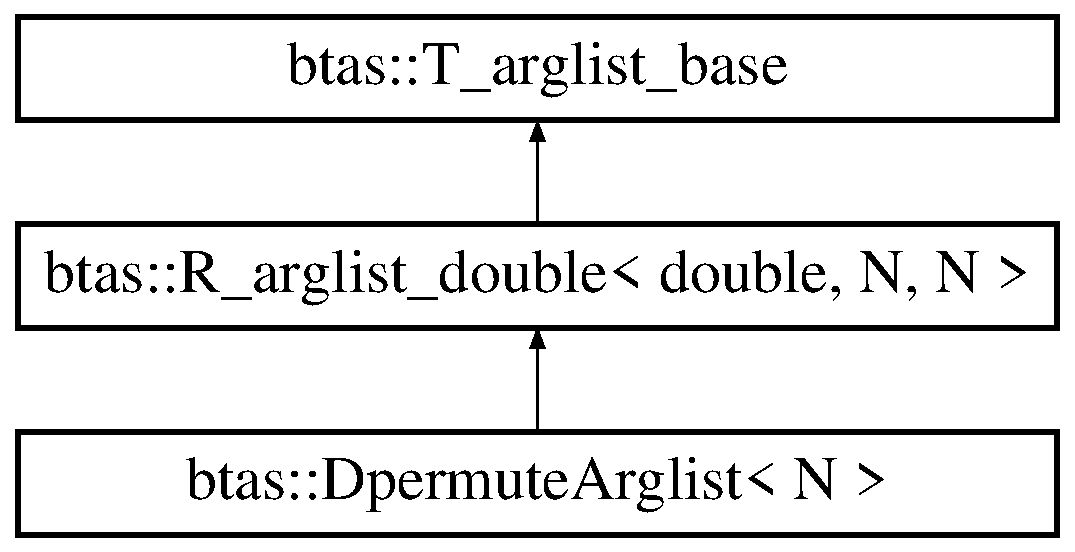
\includegraphics[height=3.000000cm]{d6/d58/classbtas_1_1DpermuteArglist}
\end{center}
\end{figure}
\subsection*{Public Member Functions}
\begin{DoxyCompactItemize}
\item 
{\bf Dpermute\-Arglist} ()
\begin{DoxyCompactList}\small\item\em Default constructor. \end{DoxyCompactList}\item 
{\bf Dpermute\-Arglist} (const shared\-\_\-ptr$<$ {\bf D\-Array}$<$ N $>$$>$ \&x\-\_\-ptr, const {\bf I\-Vector}$<$ N $>$ \&permute\-\_\-index, const shared\-\_\-ptr$<$ {\bf D\-Array}$<$ N $>$$>$ \&y\-\_\-ptr)
\begin{DoxyCompactList}\small\item\em Initializer. \end{DoxyCompactList}\item 
void {\bf reset} (const shared\-\_\-ptr$<$ {\bf D\-Array}$<$ N $>$$>$ \&x\-\_\-ptr, const {\bf I\-Vector}$<$ N $>$ \&permute\-\_\-index, const shared\-\_\-ptr$<$ {\bf D\-Array}$<$ N $>$$>$ \&y\-\_\-ptr)
\begin{DoxyCompactList}\small\item\em Reset arglist. \end{DoxyCompactList}\item 
void {\bf call} () const 
\begin{DoxyCompactList}\small\item\em Call Dpermute. \end{DoxyCompactList}\end{DoxyCompactItemize}
\subsection*{Private Attributes}
\begin{DoxyCompactItemize}
\item 
{\bf I\-Vector}$<$ N $>$ {\bf m\-\_\-permute\-\_\-index}
\end{DoxyCompactItemize}
\subsection*{Additional Inherited Members}


\subsection{Detailed Description}
\subsubsection*{template$<$size\-\_\-t N$>$class btas\-::\-Dpermute\-Arglist$<$ N $>$}



Definition at line 86 of file Darglist.\-h.



\subsection{Constructor \& Destructor Documentation}
\index{btas\-::\-Dpermute\-Arglist@{btas\-::\-Dpermute\-Arglist}!Dpermute\-Arglist@{Dpermute\-Arglist}}
\index{Dpermute\-Arglist@{Dpermute\-Arglist}!btas::DpermuteArglist@{btas\-::\-Dpermute\-Arglist}}
\subsubsection[{Dpermute\-Arglist}]{\setlength{\rightskip}{0pt plus 5cm}template$<$size\-\_\-t N$>$ {\bf btas\-::\-Dpermute\-Arglist}$<$ N $>$\-::{\bf Dpermute\-Arglist} (
\begin{DoxyParamCaption}
{}
\end{DoxyParamCaption}
)\hspace{0.3cm}{\ttfamily [inline]}}\label{d6/d58/classbtas_1_1DpermuteArglist_a62af5d6f28b698a2fa0237d325fa1bdd}


Default constructor. 



Definition at line 92 of file Darglist.\-h.

\index{btas\-::\-Dpermute\-Arglist@{btas\-::\-Dpermute\-Arglist}!Dpermute\-Arglist@{Dpermute\-Arglist}}
\index{Dpermute\-Arglist@{Dpermute\-Arglist}!btas::DpermuteArglist@{btas\-::\-Dpermute\-Arglist}}
\subsubsection[{Dpermute\-Arglist}]{\setlength{\rightskip}{0pt plus 5cm}template$<$size\-\_\-t N$>$ {\bf btas\-::\-Dpermute\-Arglist}$<$ N $>$\-::{\bf Dpermute\-Arglist} (
\begin{DoxyParamCaption}
\item[{const shared\-\_\-ptr$<$ {\bf D\-Array}$<$ N $>$$>$ \&}]{x\-\_\-ptr, }
\item[{const {\bf I\-Vector}$<$ N $>$ \&}]{permute\-\_\-index, }
\item[{const shared\-\_\-ptr$<$ {\bf D\-Array}$<$ N $>$$>$ \&}]{y\-\_\-ptr}
\end{DoxyParamCaption}
)\hspace{0.3cm}{\ttfamily [inline]}}\label{d6/d58/classbtas_1_1DpermuteArglist_a241493238d5bf927b0586c1c1d7dc87b}


Initializer. 



Definition at line 95 of file Darglist.\-h.



\subsection{Member Function Documentation}
\index{btas\-::\-Dpermute\-Arglist@{btas\-::\-Dpermute\-Arglist}!call@{call}}
\index{call@{call}!btas::DpermuteArglist@{btas\-::\-Dpermute\-Arglist}}
\subsubsection[{call}]{\setlength{\rightskip}{0pt plus 5cm}template$<$size\-\_\-t N$>$ void {\bf btas\-::\-Dpermute\-Arglist}$<$ N $>$\-::call (
\begin{DoxyParamCaption}
{}
\end{DoxyParamCaption}
) const\hspace{0.3cm}{\ttfamily [inline]}}\label{d6/d58/classbtas_1_1DpermuteArglist_a3d9eddfe6563b2138cf26ba5bceed810}


Call Dpermute. 



Definition at line 109 of file Darglist.\-h.



References btas\-::\-Dpermute(), and btas\-::\-Dpermute\-Arglist$<$ N $>$\-::m\-\_\-permute\-\_\-index.

\index{btas\-::\-Dpermute\-Arglist@{btas\-::\-Dpermute\-Arglist}!reset@{reset}}
\index{reset@{reset}!btas::DpermuteArglist@{btas\-::\-Dpermute\-Arglist}}
\subsubsection[{reset}]{\setlength{\rightskip}{0pt plus 5cm}template$<$size\-\_\-t N$>$ void {\bf btas\-::\-Dpermute\-Arglist}$<$ N $>$\-::reset (
\begin{DoxyParamCaption}
\item[{const shared\-\_\-ptr$<$ {\bf D\-Array}$<$ N $>$$>$ \&}]{x\-\_\-ptr, }
\item[{const {\bf I\-Vector}$<$ N $>$ \&}]{permute\-\_\-index, }
\item[{const shared\-\_\-ptr$<$ {\bf D\-Array}$<$ N $>$$>$ \&}]{y\-\_\-ptr}
\end{DoxyParamCaption}
)\hspace{0.3cm}{\ttfamily [inline]}}\label{d6/d58/classbtas_1_1DpermuteArglist_af8503a6b74c047066860c9906e4146a8}


Reset arglist. 



Definition at line 102 of file Darglist.\-h.



References btas\-::\-Dpermute\-Arglist$<$ N $>$\-::m\-\_\-permute\-\_\-index, and btas\-::\-R\-\_\-arglist\-\_\-double$<$ T, N1, N2 $>$\-::reset().



\subsection{Field Documentation}
\index{btas\-::\-Dpermute\-Arglist@{btas\-::\-Dpermute\-Arglist}!m\-\_\-permute\-\_\-index@{m\-\_\-permute\-\_\-index}}
\index{m\-\_\-permute\-\_\-index@{m\-\_\-permute\-\_\-index}!btas::DpermuteArglist@{btas\-::\-Dpermute\-Arglist}}
\subsubsection[{m\-\_\-permute\-\_\-index}]{\setlength{\rightskip}{0pt plus 5cm}template$<$size\-\_\-t N$>$ {\bf I\-Vector}$<$N$>$ {\bf btas\-::\-Dpermute\-Arglist}$<$ N $>$\-::m\-\_\-permute\-\_\-index\hspace{0.3cm}{\ttfamily [private]}}\label{d6/d58/classbtas_1_1DpermuteArglist_a6ce0aa13a10e6c5f1131bf8133e5407f}


Definition at line 89 of file Darglist.\-h.



Referenced by btas\-::\-Dpermute\-Arglist$<$ N $>$\-::call(), and btas\-::\-Dpermute\-Arglist$<$ N $>$\-::reset().



The documentation for this class was generated from the following file\-:\begin{DoxyCompactItemize}
\item 
include/btas/\-D\-E\-N\-S\-E/{\bf Darglist.\-h}\end{DoxyCompactItemize}

\section{btas\-:\-:Dscal\-Arglist$<$ N $>$ Class Template Reference}
\label{d0/d2f/classbtas_1_1DscalArglist}\index{btas\-::\-Dscal\-Arglist$<$ N $>$@{btas\-::\-Dscal\-Arglist$<$ N $>$}}


{\ttfamily \#include $<$Darglist.\-h$>$}

Inheritance diagram for btas\-:\-:Dscal\-Arglist$<$ N $>$\-:\begin{figure}[H]
\begin{center}
\leavevmode
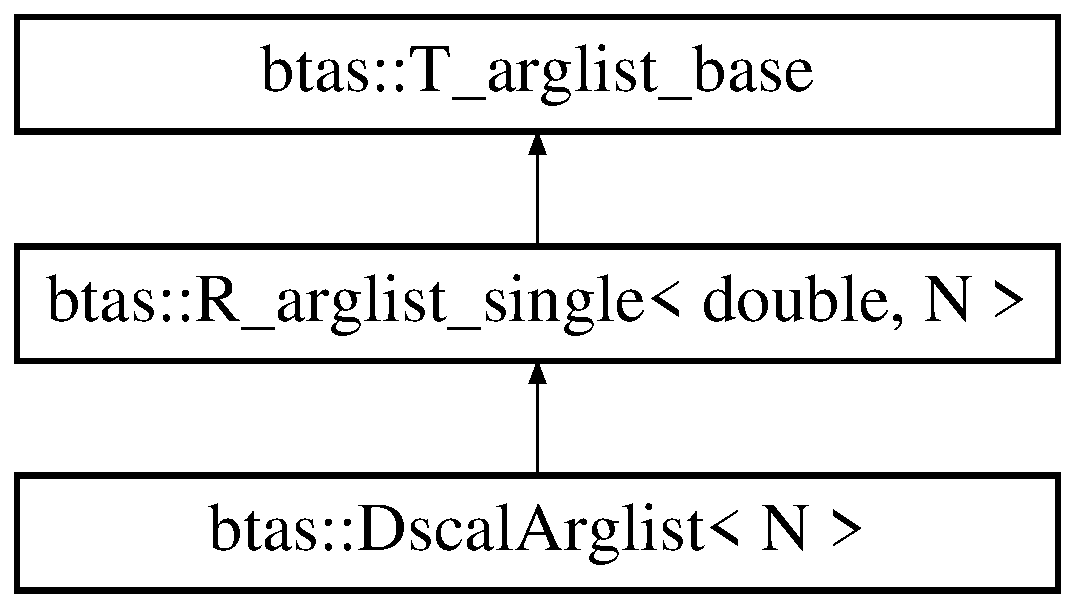
\includegraphics[height=3.000000cm]{d0/d2f/classbtas_1_1DscalArglist}
\end{center}
\end{figure}
\subsection*{Public Member Functions}
\begin{DoxyCompactItemize}
\item 
{\bf Dscal\-Arglist} ()
\begin{DoxyCompactList}\small\item\em Default constructor. \end{DoxyCompactList}\item 
{\bf Dscal\-Arglist} (const double \&alpha, const shared\-\_\-ptr$<$ {\bf D\-Array}$<$ N $>$$>$ \&x\-\_\-ptr)
\begin{DoxyCompactList}\small\item\em Initializer. \end{DoxyCompactList}\item 
void {\bf reset} (const double \&alpha, const shared\-\_\-ptr$<$ {\bf D\-Array}$<$ N $>$$>$ \&x\-\_\-ptr)
\begin{DoxyCompactList}\small\item\em Reset arglist. \end{DoxyCompactList}\item 
void {\bf call} () const 
\begin{DoxyCompactList}\small\item\em Call Dscal. \end{DoxyCompactList}\end{DoxyCompactItemize}
\subsection*{Private Attributes}
\begin{DoxyCompactItemize}
\item 
double {\bf m\-\_\-alpha}
\end{DoxyCompactItemize}
\subsection*{Additional Inherited Members}


\subsection{Detailed Description}
\subsubsection*{template$<$size\-\_\-t N$>$class btas\-::\-Dscal\-Arglist$<$ N $>$}



Definition at line 35 of file Darglist.\-h.



\subsection{Constructor \& Destructor Documentation}
\index{btas\-::\-Dscal\-Arglist@{btas\-::\-Dscal\-Arglist}!Dscal\-Arglist@{Dscal\-Arglist}}
\index{Dscal\-Arglist@{Dscal\-Arglist}!btas::DscalArglist@{btas\-::\-Dscal\-Arglist}}
\subsubsection[{Dscal\-Arglist}]{\setlength{\rightskip}{0pt plus 5cm}template$<$size\-\_\-t N$>$ {\bf btas\-::\-Dscal\-Arglist}$<$ N $>$\-::{\bf Dscal\-Arglist} (
\begin{DoxyParamCaption}
{}
\end{DoxyParamCaption}
)\hspace{0.3cm}{\ttfamily [inline]}}\label{d0/d2f/classbtas_1_1DscalArglist_ab93ebba9ed0d0e371d8ed35ca543559f}


Default constructor. 



Definition at line 41 of file Darglist.\-h.

\index{btas\-::\-Dscal\-Arglist@{btas\-::\-Dscal\-Arglist}!Dscal\-Arglist@{Dscal\-Arglist}}
\index{Dscal\-Arglist@{Dscal\-Arglist}!btas::DscalArglist@{btas\-::\-Dscal\-Arglist}}
\subsubsection[{Dscal\-Arglist}]{\setlength{\rightskip}{0pt plus 5cm}template$<$size\-\_\-t N$>$ {\bf btas\-::\-Dscal\-Arglist}$<$ N $>$\-::{\bf Dscal\-Arglist} (
\begin{DoxyParamCaption}
\item[{const double \&}]{alpha, }
\item[{const shared\-\_\-ptr$<$ {\bf D\-Array}$<$ N $>$$>$ \&}]{x\-\_\-ptr}
\end{DoxyParamCaption}
)\hspace{0.3cm}{\ttfamily [inline]}}\label{d0/d2f/classbtas_1_1DscalArglist_a2e511436d16a83d4d3dd9ce33e778737}


Initializer. 



Definition at line 44 of file Darglist.\-h.



\subsection{Member Function Documentation}
\index{btas\-::\-Dscal\-Arglist@{btas\-::\-Dscal\-Arglist}!call@{call}}
\index{call@{call}!btas::DscalArglist@{btas\-::\-Dscal\-Arglist}}
\subsubsection[{call}]{\setlength{\rightskip}{0pt plus 5cm}template$<$size\-\_\-t N$>$ void {\bf btas\-::\-Dscal\-Arglist}$<$ N $>$\-::call (
\begin{DoxyParamCaption}
{}
\end{DoxyParamCaption}
) const\hspace{0.3cm}{\ttfamily [inline]}}\label{d0/d2f/classbtas_1_1DscalArglist_acb19da019aeb588393ee760161259b37}


Call Dscal. 



Definition at line 55 of file Darglist.\-h.



References btas\-::\-Dscal(), and btas\-::\-Dscal\-Arglist$<$ N $>$\-::m\-\_\-alpha.

\index{btas\-::\-Dscal\-Arglist@{btas\-::\-Dscal\-Arglist}!reset@{reset}}
\index{reset@{reset}!btas::DscalArglist@{btas\-::\-Dscal\-Arglist}}
\subsubsection[{reset}]{\setlength{\rightskip}{0pt plus 5cm}template$<$size\-\_\-t N$>$ void {\bf btas\-::\-Dscal\-Arglist}$<$ N $>$\-::reset (
\begin{DoxyParamCaption}
\item[{const double \&}]{alpha, }
\item[{const shared\-\_\-ptr$<$ {\bf D\-Array}$<$ N $>$$>$ \&}]{x\-\_\-ptr}
\end{DoxyParamCaption}
)\hspace{0.3cm}{\ttfamily [inline]}}\label{d0/d2f/classbtas_1_1DscalArglist_ae71bc78a121a71349722a700b4f6ae1f}


Reset arglist. 



Definition at line 49 of file Darglist.\-h.



References btas\-::\-Dscal\-Arglist$<$ N $>$\-::m\-\_\-alpha, and btas\-::\-R\-\_\-arglist\-\_\-single$<$ T, N1 $>$\-::reset().



\subsection{Field Documentation}
\index{btas\-::\-Dscal\-Arglist@{btas\-::\-Dscal\-Arglist}!m\-\_\-alpha@{m\-\_\-alpha}}
\index{m\-\_\-alpha@{m\-\_\-alpha}!btas::DscalArglist@{btas\-::\-Dscal\-Arglist}}
\subsubsection[{m\-\_\-alpha}]{\setlength{\rightskip}{0pt plus 5cm}template$<$size\-\_\-t N$>$ double {\bf btas\-::\-Dscal\-Arglist}$<$ N $>$\-::m\-\_\-alpha\hspace{0.3cm}{\ttfamily [private]}}\label{d0/d2f/classbtas_1_1DscalArglist_af03624d1ff60170efb19b8d6c9d8e26e}


Definition at line 38 of file Darglist.\-h.



Referenced by btas\-::\-Dscal\-Arglist$<$ N $>$\-::call(), and btas\-::\-Dscal\-Arglist$<$ N $>$\-::reset().



The documentation for this class was generated from the following file\-:\begin{DoxyCompactItemize}
\item 
include/btas/\-D\-E\-N\-S\-E/{\bf Darglist.\-h}\end{DoxyCompactItemize}

\section{F\-C\-\_\-\-C\-O\-M\-P\-L\-E\-X\-\_\-08 Struct Reference}
\label{d4/d56/structFC__COMPLEX__08}\index{F\-C\-\_\-\-C\-O\-M\-P\-L\-E\-X\-\_\-08@{F\-C\-\_\-\-C\-O\-M\-P\-L\-E\-X\-\_\-08}}


{\ttfamily \#include $<$clapack.\-h$>$}

\subsection*{Data Fields}
\begin{DoxyCompactItemize}
\item 
float {\bf real}
\item 
float {\bf imag}
\end{DoxyCompactItemize}


\subsection{Detailed Description}


Definition at line 57 of file clapack.\-h.



\subsection{Field Documentation}
\index{F\-C\-\_\-\-C\-O\-M\-P\-L\-E\-X\-\_\-08@{F\-C\-\_\-\-C\-O\-M\-P\-L\-E\-X\-\_\-08}!imag@{imag}}
\index{imag@{imag}!FC_COMPLEX_08@{F\-C\-\_\-\-C\-O\-M\-P\-L\-E\-X\-\_\-08}}
\subsubsection[{imag}]{\setlength{\rightskip}{0pt plus 5cm}float F\-C\-\_\-\-C\-O\-M\-P\-L\-E\-X\-\_\-08\-::imag}\label{d4/d56/structFC__COMPLEX__08_abf5fdfd13f39d9fc9b055d7a83415512}


Definition at line 59 of file clapack.\-h.

\index{F\-C\-\_\-\-C\-O\-M\-P\-L\-E\-X\-\_\-08@{F\-C\-\_\-\-C\-O\-M\-P\-L\-E\-X\-\_\-08}!real@{real}}
\index{real@{real}!FC_COMPLEX_08@{F\-C\-\_\-\-C\-O\-M\-P\-L\-E\-X\-\_\-08}}
\subsubsection[{real}]{\setlength{\rightskip}{0pt plus 5cm}float F\-C\-\_\-\-C\-O\-M\-P\-L\-E\-X\-\_\-08\-::real}\label{d4/d56/structFC__COMPLEX__08_a4054ea8dd468d4c10370d337e578c16a}


Definition at line 58 of file clapack.\-h.



The documentation for this struct was generated from the following file\-:\begin{DoxyCompactItemize}
\item 
include/lapack/{\bf clapack.\-h}\end{DoxyCompactItemize}

\section{F\-C\-\_\-\-C\-O\-M\-P\-L\-E\-X\-\_\-16 Struct Reference}
\label{d5/d95/structFC__COMPLEX__16}\index{F\-C\-\_\-\-C\-O\-M\-P\-L\-E\-X\-\_\-16@{F\-C\-\_\-\-C\-O\-M\-P\-L\-E\-X\-\_\-16}}


{\ttfamily \#include $<$clapack.\-h$>$}

\subsection*{Data Fields}
\begin{DoxyCompactItemize}
\item 
double {\bf real}
\item 
double {\bf imag}
\end{DoxyCompactItemize}


\subsection{Detailed Description}


Definition at line 62 of file clapack.\-h.



\subsection{Field Documentation}
\index{F\-C\-\_\-\-C\-O\-M\-P\-L\-E\-X\-\_\-16@{F\-C\-\_\-\-C\-O\-M\-P\-L\-E\-X\-\_\-16}!imag@{imag}}
\index{imag@{imag}!FC_COMPLEX_16@{F\-C\-\_\-\-C\-O\-M\-P\-L\-E\-X\-\_\-16}}
\subsubsection[{imag}]{\setlength{\rightskip}{0pt plus 5cm}double F\-C\-\_\-\-C\-O\-M\-P\-L\-E\-X\-\_\-16\-::imag}\label{d5/d95/structFC__COMPLEX__16_a075588e4bbfd14523ef91f3d2eb460b4}


Definition at line 64 of file clapack.\-h.

\index{F\-C\-\_\-\-C\-O\-M\-P\-L\-E\-X\-\_\-16@{F\-C\-\_\-\-C\-O\-M\-P\-L\-E\-X\-\_\-16}!real@{real}}
\index{real@{real}!FC_COMPLEX_16@{F\-C\-\_\-\-C\-O\-M\-P\-L\-E\-X\-\_\-16}}
\subsubsection[{real}]{\setlength{\rightskip}{0pt plus 5cm}double F\-C\-\_\-\-C\-O\-M\-P\-L\-E\-X\-\_\-16\-::real}\label{d5/d95/structFC__COMPLEX__16_a285e27d39a7af867d2adf465dd97c724}


Definition at line 63 of file clapack.\-h.



The documentation for this struct was generated from the following file\-:\begin{DoxyCompactItemize}
\item 
include/lapack/{\bf clapack.\-h}\end{DoxyCompactItemize}

\section{btas\-:\-:indexed\-\_\-loop$<$ N $>$ Class Template Reference}
\label{d4/d84/classbtas_1_1indexed__loop}\index{btas\-::indexed\-\_\-loop$<$ N $>$@{btas\-::indexed\-\_\-loop$<$ N $>$}}


Indexed loop for array object.  




{\ttfamily \#include $<$indexed\-\_\-loop.\-h$>$}

\subsection*{Public Member Functions}
\begin{DoxyCompactItemize}
\item 
{\footnotesize template$<$size\-\_\-t M$>$ }\\{\bf indexed\-\_\-loop} (const {\bf I\-Vector}$<$ M $>$ \&first, const {\bf I\-Vector}$<$ M $>$ \&last)
\item 
{\footnotesize template$<$size\-\_\-t M$>$ }\\void {\bf reset} (const {\bf I\-Vector}$<$ M $>$ \&first, const {\bf I\-Vector}$<$ M $>$ \&last)
\item 
{\bf I\-Vector}$<$ N $>$ {\bf index} () const 
\item 
{\bf indexed\-\_\-loop} \& {\bf operator++} ()
\item 
bool {\bf end} () const 
\end{DoxyCompactItemize}
\subsection*{Private Member Functions}
\begin{DoxyCompactItemize}
\item 
{\footnotesize template$<$size\-\_\-t M$>$ }\\void {\bf make\-\_\-index} ({\bf I\-Vector}$<$ M $>$ \&{\bf index}) const 
\end{DoxyCompactItemize}
\subsection*{Private Attributes}
\begin{DoxyCompactItemize}
\item 
{\bf indexed\-\_\-loop}$<$ N-\/1 $>$ {\bf m\-\_\-oloop}
\item 
int {\bf m\-\_\-index}
\item 
int {\bf m\-\_\-first}
\item 
int {\bf m\-\_\-last}
\end{DoxyCompactItemize}
\subsection*{Friends}
\begin{DoxyCompactItemize}
\item 
class {\bf indexed\-\_\-loop$<$ N+1 $>$}
\end{DoxyCompactItemize}


\subsection{Detailed Description}
\subsubsection*{template$<$size\-\_\-t N$>$class btas\-::indexed\-\_\-loop$<$ N $>$}

Indexed loop for array object. 

\begin{DoxyParagraph}{Purpose\-:}
Let multiple for loop, e.\-g. \begin{DoxyVerb} for(int i = 0; i < Ni; ++i) {
   for(int j = 0; j < Nj; ++j) {
     for(int k = 0; k < Nk; ++k) {
       ... do something ...
     }
   }
 }
\end{DoxyVerb}

\end{DoxyParagraph}
be a single loop, i.\-e. \begin{DoxyVerb} for(indexed_loop<3> loop(make_array(0,0,0), make_array(Ni,Nj,Nk)); !loop.end(); ++loop) {
   IVector<3> index = loop.index();
   int i = index[0];
   int j = index[1];
   int k = index[2];
   ... do something ...
\end{DoxyVerb}
 

Definition at line 31 of file indexed\-\_\-loop.\-h.



\subsection{Constructor \& Destructor Documentation}
\index{btas\-::indexed\-\_\-loop@{btas\-::indexed\-\_\-loop}!indexed\-\_\-loop@{indexed\-\_\-loop}}
\index{indexed\-\_\-loop@{indexed\-\_\-loop}!btas::indexed_loop@{btas\-::indexed\-\_\-loop}}
\subsubsection[{indexed\-\_\-loop}]{\setlength{\rightskip}{0pt plus 5cm}template$<$size\-\_\-t N$>$ template$<$size\-\_\-t M$>$ {\bf btas\-::indexed\-\_\-loop}$<$ N $>$\-::{\bf indexed\-\_\-loop} (
\begin{DoxyParamCaption}
\item[{const {\bf I\-Vector}$<$ M $>$ \&}]{first, }
\item[{const {\bf I\-Vector}$<$ M $>$ \&}]{last}
\end{DoxyParamCaption}
)\hspace{0.3cm}{\ttfamily [inline]}}\label{d4/d84/classbtas_1_1indexed__loop_a25a0a14cd48eb06eb9c6e550743ece26}


Definition at line 43 of file indexed\-\_\-loop.\-h.



\subsection{Member Function Documentation}
\index{btas\-::indexed\-\_\-loop@{btas\-::indexed\-\_\-loop}!end@{end}}
\index{end@{end}!btas::indexed_loop@{btas\-::indexed\-\_\-loop}}
\subsubsection[{end}]{\setlength{\rightskip}{0pt plus 5cm}template$<$size\-\_\-t N$>$ bool {\bf btas\-::indexed\-\_\-loop}$<$ N $>$\-::end (
\begin{DoxyParamCaption}
{}
\end{DoxyParamCaption}
) const\hspace{0.3cm}{\ttfamily [inline]}}\label{d4/d84/classbtas_1_1indexed__loop_a4804caf77a04b21457f69bcf68e18798}


Definition at line 68 of file indexed\-\_\-loop.\-h.



References btas\-::indexed\-\_\-loop$<$ N $>$\-::m\-\_\-oloop.

\index{btas\-::indexed\-\_\-loop@{btas\-::indexed\-\_\-loop}!index@{index}}
\index{index@{index}!btas::indexed_loop@{btas\-::indexed\-\_\-loop}}
\subsubsection[{index}]{\setlength{\rightskip}{0pt plus 5cm}template$<$size\-\_\-t N$>$ {\bf I\-Vector}$<$N$>$ {\bf btas\-::indexed\-\_\-loop}$<$ N $>$\-::index (
\begin{DoxyParamCaption}
{}
\end{DoxyParamCaption}
) const\hspace{0.3cm}{\ttfamily [inline]}}\label{d4/d84/classbtas_1_1indexed__loop_ab580f85cde71209f62f63c7092c9f036}


Definition at line 54 of file indexed\-\_\-loop.\-h.



References btas\-::indexed\-\_\-loop$<$ N $>$\-::make\-\_\-index().

\index{btas\-::indexed\-\_\-loop@{btas\-::indexed\-\_\-loop}!make\-\_\-index@{make\-\_\-index}}
\index{make\-\_\-index@{make\-\_\-index}!btas::indexed_loop@{btas\-::indexed\-\_\-loop}}
\subsubsection[{make\-\_\-index}]{\setlength{\rightskip}{0pt plus 5cm}template$<$size\-\_\-t N$>$ template$<$size\-\_\-t M$>$ void {\bf btas\-::indexed\-\_\-loop}$<$ N $>$\-::make\-\_\-index (
\begin{DoxyParamCaption}
\item[{{\bf I\-Vector}$<$ M $>$ \&}]{index}
\end{DoxyParamCaption}
) const\hspace{0.3cm}{\ttfamily [inline]}, {\ttfamily [private]}}\label{d4/d84/classbtas_1_1indexed__loop_a0fcb4bddd3ab4fa11646588895923dea}


Definition at line 36 of file indexed\-\_\-loop.\-h.



References btas\-::indexed\-\_\-loop$<$ N $>$\-::m\-\_\-index, and btas\-::indexed\-\_\-loop$<$ N $>$\-::m\-\_\-oloop.



Referenced by btas\-::indexed\-\_\-loop$<$ N $>$\-::index().

\index{btas\-::indexed\-\_\-loop@{btas\-::indexed\-\_\-loop}!operator++@{operator++}}
\index{operator++@{operator++}!btas::indexed_loop@{btas\-::indexed\-\_\-loop}}
\subsubsection[{operator++}]{\setlength{\rightskip}{0pt plus 5cm}template$<$size\-\_\-t N$>$ {\bf indexed\-\_\-loop}\& {\bf btas\-::indexed\-\_\-loop}$<$ N $>$\-::operator++ (
\begin{DoxyParamCaption}
{}
\end{DoxyParamCaption}
)\hspace{0.3cm}{\ttfamily [inline]}}\label{d4/d84/classbtas_1_1indexed__loop_a46e026728aaadb497a8f29dc41d5803a}


Definition at line 60 of file indexed\-\_\-loop.\-h.



References btas\-::indexed\-\_\-loop$<$ N $>$\-::m\-\_\-first, btas\-::indexed\-\_\-loop$<$ N $>$\-::m\-\_\-index, btas\-::indexed\-\_\-loop$<$ N $>$\-::m\-\_\-last, and btas\-::indexed\-\_\-loop$<$ N $>$\-::m\-\_\-oloop.

\index{btas\-::indexed\-\_\-loop@{btas\-::indexed\-\_\-loop}!reset@{reset}}
\index{reset@{reset}!btas::indexed_loop@{btas\-::indexed\-\_\-loop}}
\subsubsection[{reset}]{\setlength{\rightskip}{0pt plus 5cm}template$<$size\-\_\-t N$>$ template$<$size\-\_\-t M$>$ void {\bf btas\-::indexed\-\_\-loop}$<$ N $>$\-::reset (
\begin{DoxyParamCaption}
\item[{const {\bf I\-Vector}$<$ M $>$ \&}]{first, }
\item[{const {\bf I\-Vector}$<$ M $>$ \&}]{last}
\end{DoxyParamCaption}
)\hspace{0.3cm}{\ttfamily [inline]}}\label{d4/d84/classbtas_1_1indexed__loop_a1a876a0677fc049ac8681ec50c21629c}


Definition at line 47 of file indexed\-\_\-loop.\-h.



References btas\-::indexed\-\_\-loop$<$ N $>$\-::m\-\_\-first, btas\-::indexed\-\_\-loop$<$ N $>$\-::m\-\_\-index, btas\-::indexed\-\_\-loop$<$ N $>$\-::m\-\_\-last, and btas\-::indexed\-\_\-loop$<$ N $>$\-::m\-\_\-oloop.



\subsection{Friends And Related Function Documentation}
\index{btas\-::indexed\-\_\-loop@{btas\-::indexed\-\_\-loop}!indexed\-\_\-loop$<$ N+1 $>$@{indexed\-\_\-loop$<$ N+1 $>$}}
\index{indexed\-\_\-loop$<$ N+1 $>$@{indexed\-\_\-loop$<$ N+1 $>$}!btas::indexed_loop@{btas\-::indexed\-\_\-loop}}
\subsubsection[{indexed\-\_\-loop$<$ N+1 $>$}]{\setlength{\rightskip}{0pt plus 5cm}template$<$size\-\_\-t N$>$ friend class {\bf indexed\-\_\-loop}$<$ N+1 $>$\hspace{0.3cm}{\ttfamily [friend]}}\label{d4/d84/classbtas_1_1indexed__loop_aab14324e199b0a7abda57cd40e214f8a}


Definition at line 33 of file indexed\-\_\-loop.\-h.



\subsection{Field Documentation}
\index{btas\-::indexed\-\_\-loop@{btas\-::indexed\-\_\-loop}!m\-\_\-first@{m\-\_\-first}}
\index{m\-\_\-first@{m\-\_\-first}!btas::indexed_loop@{btas\-::indexed\-\_\-loop}}
\subsubsection[{m\-\_\-first}]{\setlength{\rightskip}{0pt plus 5cm}template$<$size\-\_\-t N$>$ int {\bf btas\-::indexed\-\_\-loop}$<$ N $>$\-::m\-\_\-first\hspace{0.3cm}{\ttfamily [private]}}\label{d4/d84/classbtas_1_1indexed__loop_a83e9fc43c8d7f22adcec5869e05ecdd0}


Definition at line 76 of file indexed\-\_\-loop.\-h.



Referenced by btas\-::indexed\-\_\-loop$<$ N $>$\-::operator++(), btas\-::indexed\-\_\-loop$<$ 1 $>$\-::operator++(), btas\-::indexed\-\_\-loop$<$ N $>$\-::reset(), and btas\-::indexed\-\_\-loop$<$ 1 $>$\-::reset().

\index{btas\-::indexed\-\_\-loop@{btas\-::indexed\-\_\-loop}!m\-\_\-index@{m\-\_\-index}}
\index{m\-\_\-index@{m\-\_\-index}!btas::indexed_loop@{btas\-::indexed\-\_\-loop}}
\subsubsection[{m\-\_\-index}]{\setlength{\rightskip}{0pt plus 5cm}template$<$size\-\_\-t N$>$ int {\bf btas\-::indexed\-\_\-loop}$<$ N $>$\-::m\-\_\-index\hspace{0.3cm}{\ttfamily [private]}}\label{d4/d84/classbtas_1_1indexed__loop_ac53c3f4465df4baf4b8cc0f9f3824f68}


Definition at line 74 of file indexed\-\_\-loop.\-h.



Referenced by btas\-::indexed\-\_\-loop$<$ 1 $>$\-::index(), btas\-::indexed\-\_\-loop$<$ N $>$\-::make\-\_\-index(), btas\-::indexed\-\_\-loop$<$ 1 $>$\-::make\-\_\-index(), btas\-::indexed\-\_\-loop$<$ N $>$\-::operator++(), btas\-::indexed\-\_\-loop$<$ 1 $>$\-::operator++(), btas\-::indexed\-\_\-loop$<$ N $>$\-::reset(), and btas\-::indexed\-\_\-loop$<$ 1 $>$\-::reset().

\index{btas\-::indexed\-\_\-loop@{btas\-::indexed\-\_\-loop}!m\-\_\-last@{m\-\_\-last}}
\index{m\-\_\-last@{m\-\_\-last}!btas::indexed_loop@{btas\-::indexed\-\_\-loop}}
\subsubsection[{m\-\_\-last}]{\setlength{\rightskip}{0pt plus 5cm}template$<$size\-\_\-t N$>$ int {\bf btas\-::indexed\-\_\-loop}$<$ N $>$\-::m\-\_\-last\hspace{0.3cm}{\ttfamily [private]}}\label{d4/d84/classbtas_1_1indexed__loop_a19e3b5fe0657aeb3f849ac9ca11c8d44}


Definition at line 78 of file indexed\-\_\-loop.\-h.



Referenced by btas\-::indexed\-\_\-loop$<$ N $>$\-::operator++(), btas\-::indexed\-\_\-loop$<$ 1 $>$\-::operator++(), btas\-::indexed\-\_\-loop$<$ N $>$\-::reset(), and btas\-::indexed\-\_\-loop$<$ 1 $>$\-::reset().

\index{btas\-::indexed\-\_\-loop@{btas\-::indexed\-\_\-loop}!m\-\_\-oloop@{m\-\_\-oloop}}
\index{m\-\_\-oloop@{m\-\_\-oloop}!btas::indexed_loop@{btas\-::indexed\-\_\-loop}}
\subsubsection[{m\-\_\-oloop}]{\setlength{\rightskip}{0pt plus 5cm}template$<$size\-\_\-t N$>$ {\bf indexed\-\_\-loop}$<$N-\/1$>$ {\bf btas\-::indexed\-\_\-loop}$<$ N $>$\-::m\-\_\-oloop\hspace{0.3cm}{\ttfamily [private]}}\label{d4/d84/classbtas_1_1indexed__loop_a1822b86cdcb21caa943d899109a786ec}


Definition at line 72 of file indexed\-\_\-loop.\-h.



Referenced by btas\-::indexed\-\_\-loop$<$ N $>$\-::end(), btas\-::indexed\-\_\-loop$<$ N $>$\-::make\-\_\-index(), btas\-::indexed\-\_\-loop$<$ N $>$\-::operator++(), and btas\-::indexed\-\_\-loop$<$ N $>$\-::reset().



The documentation for this class was generated from the following file\-:\begin{DoxyCompactItemize}
\item 
include/{\bf indexed\-\_\-loop.\-h}\end{DoxyCompactItemize}

\section{btas\-:\-:indexed\-\_\-loop$<$ 1 $>$ Class Template Reference}
\label{d7/d39/classbtas_1_1indexed__loop_3_011_01_4}\index{btas\-::indexed\-\_\-loop$<$ 1 $>$@{btas\-::indexed\-\_\-loop$<$ 1 $>$}}


{\ttfamily \#include $<$indexed\-\_\-loop.\-h$>$}

\subsection*{Public Member Functions}
\begin{DoxyCompactItemize}
\item 
{\footnotesize template$<$size\-\_\-t M$>$ }\\{\bf indexed\-\_\-loop} (const {\bf I\-Vector}$<$ M $>$ \&first, const {\bf I\-Vector}$<$ M $>$ \&last)
\item 
{\footnotesize template$<$size\-\_\-t M$>$ }\\void {\bf reset} (const {\bf I\-Vector}$<$ M $>$ \&first, const {\bf I\-Vector}$<$ M $>$ \&last)
\item 
{\bf I\-Vector}$<$ 1 $>$ {\bf index} () const 
\item 
{\bf indexed\-\_\-loop} \& {\bf operator++} ()
\item 
bool {\bf end} () const 
\end{DoxyCompactItemize}
\subsection*{Private Member Functions}
\begin{DoxyCompactItemize}
\item 
{\footnotesize template$<$size\-\_\-t M$>$ }\\void {\bf make\-\_\-index} ({\bf I\-Vector}$<$ M $>$ \&{\bf index}) const 
\end{DoxyCompactItemize}
\subsection*{Private Attributes}
\begin{DoxyCompactItemize}
\item 
int {\bf m\-\_\-index}
\item 
int {\bf m\-\_\-first}
\item 
int {\bf m\-\_\-last}
\item 
bool {\bf m\-\_\-end}
\end{DoxyCompactItemize}
\subsection*{Friends}
\begin{DoxyCompactItemize}
\item 
class {\bf indexed\-\_\-loop$<$ 2 $>$}
\end{DoxyCompactItemize}


\subsection{Detailed Description}
\subsubsection*{template$<$$>$class btas\-::indexed\-\_\-loop$<$ 1 $>$}



Definition at line 82 of file indexed\-\_\-loop.\-h.



\subsection{Constructor \& Destructor Documentation}
\index{btas\-::indexed\-\_\-loop$<$ 1 $>$@{btas\-::indexed\-\_\-loop$<$ 1 $>$}!indexed\-\_\-loop@{indexed\-\_\-loop}}
\index{indexed\-\_\-loop@{indexed\-\_\-loop}!btas::indexed_loop< 1 >@{btas\-::indexed\-\_\-loop$<$ 1 $>$}}
\subsubsection[{indexed\-\_\-loop}]{\setlength{\rightskip}{0pt plus 5cm}template$<$size\-\_\-t M$>$ {\bf btas\-::indexed\-\_\-loop}$<$ 1 $>$\-::{\bf indexed\-\_\-loop} (
\begin{DoxyParamCaption}
\item[{const {\bf I\-Vector}$<$ M $>$ \&}]{first, }
\item[{const {\bf I\-Vector}$<$ M $>$ \&}]{last}
\end{DoxyParamCaption}
)\hspace{0.3cm}{\ttfamily [inline]}}\label{d7/d39/classbtas_1_1indexed__loop_3_011_01_4_a89d16d161715a83f0620963d4fa49476}


Definition at line 91 of file indexed\-\_\-loop.\-h.



\subsection{Member Function Documentation}
\index{btas\-::indexed\-\_\-loop$<$ 1 $>$@{btas\-::indexed\-\_\-loop$<$ 1 $>$}!end@{end}}
\index{end@{end}!btas::indexed_loop< 1 >@{btas\-::indexed\-\_\-loop$<$ 1 $>$}}
\subsubsection[{end}]{\setlength{\rightskip}{0pt plus 5cm}bool {\bf btas\-::indexed\-\_\-loop}$<$ 1 $>$\-::end (
\begin{DoxyParamCaption}
{}
\end{DoxyParamCaption}
) const\hspace{0.3cm}{\ttfamily [inline]}}\label{d7/d39/classbtas_1_1indexed__loop_3_011_01_4_a376ea72eb7f2b25084c74dda11fe76a9}


Definition at line 115 of file indexed\-\_\-loop.\-h.

\index{btas\-::indexed\-\_\-loop$<$ 1 $>$@{btas\-::indexed\-\_\-loop$<$ 1 $>$}!index@{index}}
\index{index@{index}!btas::indexed_loop< 1 >@{btas\-::indexed\-\_\-loop$<$ 1 $>$}}
\subsubsection[{index}]{\setlength{\rightskip}{0pt plus 5cm}{\bf I\-Vector}$<$1$>$ {\bf btas\-::indexed\-\_\-loop}$<$ 1 $>$\-::index (
\begin{DoxyParamCaption}
{}
\end{DoxyParamCaption}
) const\hspace{0.3cm}{\ttfamily [inline]}}\label{d7/d39/classbtas_1_1indexed__loop_3_011_01_4_a5855f2d75d284bc375091bf7e744b119}


Definition at line 102 of file indexed\-\_\-loop.\-h.



References btas\-::indexed\-\_\-loop$<$ N $>$\-::m\-\_\-index.

\index{btas\-::indexed\-\_\-loop$<$ 1 $>$@{btas\-::indexed\-\_\-loop$<$ 1 $>$}!make\-\_\-index@{make\-\_\-index}}
\index{make\-\_\-index@{make\-\_\-index}!btas::indexed_loop< 1 >@{btas\-::indexed\-\_\-loop$<$ 1 $>$}}
\subsubsection[{make\-\_\-index}]{\setlength{\rightskip}{0pt plus 5cm}template$<$size\-\_\-t M$>$ void {\bf btas\-::indexed\-\_\-loop}$<$ 1 $>$\-::make\-\_\-index (
\begin{DoxyParamCaption}
\item[{{\bf I\-Vector}$<$ M $>$ \&}]{index}
\end{DoxyParamCaption}
) const\hspace{0.3cm}{\ttfamily [inline]}, {\ttfamily [private]}}\label{d7/d39/classbtas_1_1indexed__loop_3_011_01_4_a20ed1499c7f31db20f08d538ab869490}


Definition at line 87 of file indexed\-\_\-loop.\-h.



References btas\-::indexed\-\_\-loop$<$ N $>$\-::m\-\_\-index.

\index{btas\-::indexed\-\_\-loop$<$ 1 $>$@{btas\-::indexed\-\_\-loop$<$ 1 $>$}!operator++@{operator++}}
\index{operator++@{operator++}!btas::indexed_loop< 1 >@{btas\-::indexed\-\_\-loop$<$ 1 $>$}}
\subsubsection[{operator++}]{\setlength{\rightskip}{0pt plus 5cm}{\bf indexed\-\_\-loop}\& {\bf btas\-::indexed\-\_\-loop}$<$ 1 $>$\-::operator++ (
\begin{DoxyParamCaption}
{}
\end{DoxyParamCaption}
)\hspace{0.3cm}{\ttfamily [inline]}}\label{d7/d39/classbtas_1_1indexed__loop_3_011_01_4_a0479727ec9e0b8603a9af87a0bbf2ef4}


Definition at line 107 of file indexed\-\_\-loop.\-h.



References btas\-::indexed\-\_\-loop$<$ N $>$\-::m\-\_\-first, btas\-::indexed\-\_\-loop$<$ N $>$\-::m\-\_\-index, and btas\-::indexed\-\_\-loop$<$ N $>$\-::m\-\_\-last.

\index{btas\-::indexed\-\_\-loop$<$ 1 $>$@{btas\-::indexed\-\_\-loop$<$ 1 $>$}!reset@{reset}}
\index{reset@{reset}!btas::indexed_loop< 1 >@{btas\-::indexed\-\_\-loop$<$ 1 $>$}}
\subsubsection[{reset}]{\setlength{\rightskip}{0pt plus 5cm}template$<$size\-\_\-t M$>$ void {\bf btas\-::indexed\-\_\-loop}$<$ 1 $>$\-::reset (
\begin{DoxyParamCaption}
\item[{const {\bf I\-Vector}$<$ M $>$ \&}]{first, }
\item[{const {\bf I\-Vector}$<$ M $>$ \&}]{last}
\end{DoxyParamCaption}
)\hspace{0.3cm}{\ttfamily [inline]}}\label{d7/d39/classbtas_1_1indexed__loop_3_011_01_4_a87b8b1a297d66a81604b62f469745f56}


Definition at line 95 of file indexed\-\_\-loop.\-h.



References btas\-::indexed\-\_\-loop$<$ N $>$\-::m\-\_\-first, btas\-::indexed\-\_\-loop$<$ N $>$\-::m\-\_\-index, and btas\-::indexed\-\_\-loop$<$ N $>$\-::m\-\_\-last.



\subsection{Friends And Related Function Documentation}
\index{btas\-::indexed\-\_\-loop$<$ 1 $>$@{btas\-::indexed\-\_\-loop$<$ 1 $>$}!indexed\-\_\-loop$<$ 2 $>$@{indexed\-\_\-loop$<$ 2 $>$}}
\index{indexed\-\_\-loop$<$ 2 $>$@{indexed\-\_\-loop$<$ 2 $>$}!btas::indexed_loop< 1 >@{btas\-::indexed\-\_\-loop$<$ 1 $>$}}
\subsubsection[{indexed\-\_\-loop$<$ 2 $>$}]{\setlength{\rightskip}{0pt plus 5cm}friend class {\bf indexed\-\_\-loop}$<$ 2 $>$\hspace{0.3cm}{\ttfamily [friend]}}\label{d7/d39/classbtas_1_1indexed__loop_3_011_01_4_a9e5c385cfa131dd857f234a327cb5af4}


Definition at line 84 of file indexed\-\_\-loop.\-h.



\subsection{Field Documentation}
\index{btas\-::indexed\-\_\-loop$<$ 1 $>$@{btas\-::indexed\-\_\-loop$<$ 1 $>$}!m\-\_\-end@{m\-\_\-end}}
\index{m\-\_\-end@{m\-\_\-end}!btas::indexed_loop< 1 >@{btas\-::indexed\-\_\-loop$<$ 1 $>$}}
\subsubsection[{m\-\_\-end}]{\setlength{\rightskip}{0pt plus 5cm}bool {\bf btas\-::indexed\-\_\-loop}$<$ 1 $>$\-::m\-\_\-end\hspace{0.3cm}{\ttfamily [private]}}\label{d7/d39/classbtas_1_1indexed__loop_3_011_01_4_a9fcdd8a2a2f3340c12dcc2da485ee11c}


Definition at line 125 of file indexed\-\_\-loop.\-h.

\index{btas\-::indexed\-\_\-loop$<$ 1 $>$@{btas\-::indexed\-\_\-loop$<$ 1 $>$}!m\-\_\-first@{m\-\_\-first}}
\index{m\-\_\-first@{m\-\_\-first}!btas::indexed_loop< 1 >@{btas\-::indexed\-\_\-loop$<$ 1 $>$}}
\subsubsection[{m\-\_\-first}]{\setlength{\rightskip}{0pt plus 5cm}int {\bf btas\-::indexed\-\_\-loop}$<$ 1 $>$\-::m\-\_\-first\hspace{0.3cm}{\ttfamily [private]}}\label{d7/d39/classbtas_1_1indexed__loop_3_011_01_4_a3a72cf5df038567149b0c95da69ad71a}


Definition at line 121 of file indexed\-\_\-loop.\-h.

\index{btas\-::indexed\-\_\-loop$<$ 1 $>$@{btas\-::indexed\-\_\-loop$<$ 1 $>$}!m\-\_\-index@{m\-\_\-index}}
\index{m\-\_\-index@{m\-\_\-index}!btas::indexed_loop< 1 >@{btas\-::indexed\-\_\-loop$<$ 1 $>$}}
\subsubsection[{m\-\_\-index}]{\setlength{\rightskip}{0pt plus 5cm}int {\bf btas\-::indexed\-\_\-loop}$<$ 1 $>$\-::m\-\_\-index\hspace{0.3cm}{\ttfamily [private]}}\label{d7/d39/classbtas_1_1indexed__loop_3_011_01_4_a311f84ab1d0b869259e3545bfc9c540c}


Definition at line 119 of file indexed\-\_\-loop.\-h.

\index{btas\-::indexed\-\_\-loop$<$ 1 $>$@{btas\-::indexed\-\_\-loop$<$ 1 $>$}!m\-\_\-last@{m\-\_\-last}}
\index{m\-\_\-last@{m\-\_\-last}!btas::indexed_loop< 1 >@{btas\-::indexed\-\_\-loop$<$ 1 $>$}}
\subsubsection[{m\-\_\-last}]{\setlength{\rightskip}{0pt plus 5cm}int {\bf btas\-::indexed\-\_\-loop}$<$ 1 $>$\-::m\-\_\-last\hspace{0.3cm}{\ttfamily [private]}}\label{d7/d39/classbtas_1_1indexed__loop_3_011_01_4_a8d50709c833bf8e0252d4e3319655909}


Definition at line 123 of file indexed\-\_\-loop.\-h.



The documentation for this class was generated from the following file\-:\begin{DoxyCompactItemize}
\item 
include/{\bf indexed\-\_\-loop.\-h}\end{DoxyCompactItemize}

\section{btas\-:\-:null\-\_\-deleter Struct Reference}
\label{d8/d8a/structbtas_1_1null__deleter}\index{btas\-::null\-\_\-deleter@{btas\-::null\-\_\-deleter}}


Null-\/deleter.  




{\ttfamily \#include $<$btas.\-h$>$}

\subsection*{Public Member Functions}
\begin{DoxyCompactItemize}
\item 
void {\bf operator()} (void const $\ast$) const 
\end{DoxyCompactItemize}


\subsection{Detailed Description}
Null-\/deleter. 

Definition at line 44 of file btas.\-h.



\subsection{Member Function Documentation}
\index{btas\-::null\-\_\-deleter@{btas\-::null\-\_\-deleter}!operator()@{operator()}}
\index{operator()@{operator()}!btas::null_deleter@{btas\-::null\-\_\-deleter}}
\subsubsection[{operator()}]{\setlength{\rightskip}{0pt plus 5cm}void btas\-::null\-\_\-deleter\-::operator() (
\begin{DoxyParamCaption}
\item[{void const $\ast$}]{}
\end{DoxyParamCaption}
) const\hspace{0.3cm}{\ttfamily [inline]}}\label{d8/d8a/structbtas_1_1null__deleter_a712df3cbc0d96e377a68938284e08830}


Definition at line 45 of file btas.\-h.



The documentation for this struct was generated from the following file\-:\begin{DoxyCompactItemize}
\item 
include/btas/{\bf btas.\-h}\end{DoxyCompactItemize}

\section{btas\-:\-:Qshapes$<$ Q $>$ Class Template Reference}
\label{dd/df1/classbtas_1_1Qshapes}\index{btas\-::\-Qshapes$<$ Q $>$@{btas\-::\-Qshapes$<$ Q $>$}}


\doxyref{Quantum}{p.}{d8/df8/classQuantum} number vector.  




{\ttfamily \#include $<$Qshapes.\-h$>$}

Inheritance diagram for btas\-:\-:Qshapes$<$ Q $>$\-:\begin{figure}[H]
\begin{center}
\leavevmode
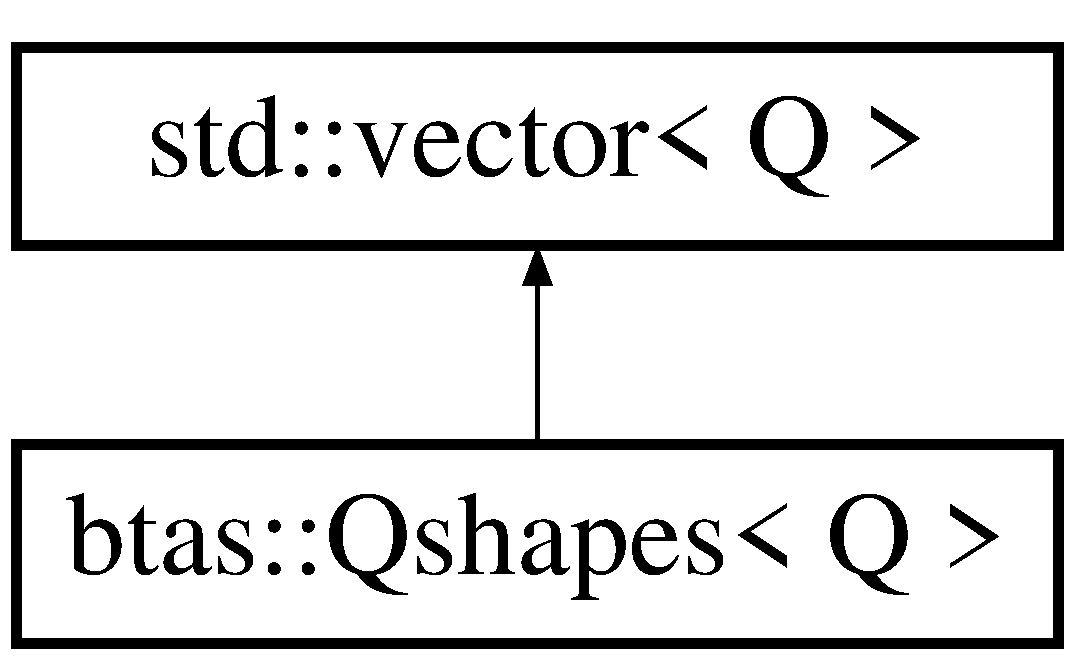
\includegraphics[height=2.000000cm]{dd/df1/classbtas_1_1Qshapes}
\end{center}
\end{figure}
\subsection*{Public Types}
\begin{DoxyCompactItemize}
\item 
typedef std\-::vector$<$ Q $>$\\*
\-::{\bf value\-\_\-type} {\bf value\-\_\-type}
\item 
typedef std\-::vector$<$ Q $>$\-::{\bf size\-\_\-type} {\bf size\-\_\-type}
\item 
typedef std\-::vector$<$ Q $>$\-::{\bf iterator} {\bf iterator}
\item 
typedef std\-::vector$<$ Q $>$\\*
\-::{\bf const\-\_\-iterator} {\bf const\-\_\-iterator}
\end{DoxyCompactItemize}
\subsection*{Public Member Functions}
\begin{DoxyCompactItemize}
\item 
{\bf Qshapes} ()
\item 
{\bf Qshapes} ({\bf size\-\_\-type} n)
\item 
{\bf Qshapes} ({\bf size\-\_\-type} n, const {\bf value\-\_\-type} \&val)
\item 
{\footnotesize template$<$class Input\-Iterator $>$ }\\{\bf Qshapes} (Input\-Iterator first, Input\-Iterator last)
\item 
{\bf Qshapes} (const {\bf Qshapes} \&x)
\item 
{\bf Qshapes} ({\bf Qshapes} \&\&x)
\item 
{\bf Qshapes} (std\-::initializer\-\_\-list$<$ {\bf value\-\_\-type} $>$ il)
\item 
{\bf $\sim$\-Qshapes} ()
\item 
{\bf Qshapes} \& {\bf operator=} (const {\bf Qshapes} \&other)
\begin{DoxyCompactList}\small\item\em Copy assignment operator. \end{DoxyCompactList}\item 
{\bf Qshapes} \& {\bf operator=} ({\bf Qshapes} \&\&other)
\begin{DoxyCompactList}\small\item\em Move assignment operator. \end{DoxyCompactList}\item 
{\bf Qshapes} {\bf operator$\ast$} (const {\bf Qshapes} \&other) const 
\begin{DoxyCompactList}\small\item\em Contract two quantum numbers\-: \{ q(ij) \-: q(i) $\ast$ q(j) \}. \end{DoxyCompactList}\item 
{\bf Qshapes} {\bf operator\&} (const {\bf Qshapes} \&other) const 
\begin{DoxyCompactList}\small\item\em Contract two quantum numbers and chose unique quantum numbers\-: \{ q(ij) \-: q(i) $\ast$ q(j) \} =$>$ \{ q(st) \}. \end{DoxyCompactList}\item 
{\bf Qshapes} {\bf operator+} (const {\bf Qshapes} \&other) const 
\begin{DoxyCompactList}\small\item\em Adding other \doxyref{Qshapes}{p.}{dd/df1/classbtas_1_1Qshapes}. \end{DoxyCompactList}\item 
{\bf Qshapes} \& {\bf operator+=} (const {\bf Qshapes} \&other)
\begin{DoxyCompactList}\small\item\em Adding other \doxyref{Qshapes}{p.}{dd/df1/classbtas_1_1Qshapes} to this. \end{DoxyCompactList}\item 
{\bf Qshapes} {\bf operator+} () const 
\begin{DoxyCompactList}\small\item\em Return copy of this. \end{DoxyCompactList}\item 
{\bf Qshapes} {\bf operator-\/} () const 
\begin{DoxyCompactList}\small\item\em Return conjugated quantum numbers. \end{DoxyCompactList}\end{DoxyCompactItemize}
\subsection*{Private Member Functions}
\begin{DoxyCompactItemize}
\item 
{\footnotesize template$<$class Archive $>$ }\\void {\bf serialize} (Archive \&ar, const unsigned int version)
\begin{DoxyCompactList}\small\item\em Boost serialization. \end{DoxyCompactList}\end{DoxyCompactItemize}
\subsection*{Friends}
\begin{DoxyCompactItemize}
\item 
class {\bf boost\-::serialization\-::access}
\end{DoxyCompactItemize}


\subsection{Detailed Description}
\subsubsection*{template$<$class Q = Quantum$>$class btas\-::\-Qshapes$<$ Q $>$}

\doxyref{Quantum}{p.}{d8/df8/classQuantum} number vector. 

Since typedef of std\-::vector$<$\-Q$>$ is ambiguous to define operators, it's implemented as a different class in terms of std\-::vector$<$\-Q$>$.

class Q must have overloaded operators\-: =, + (unary), -\/ (unary), $\ast$, ==, !=, $<$, $>$ It's also required,
\begin{DoxyItemize}
\item const static function Q\-::zero() which gives zero quantum number,
\item boolian function parity() gives true when it has odd particle number in the case of fermion
\item and, clebsch() which gives Clebsch-\/\-Gordan coefficient in the case non-\/\-Abelian symmetry
\end{DoxyItemize}

Default quantum number class is named by 'btas\-::\-Quantum' 

Definition at line 33 of file Qshapes.\-h.



\subsection{Member Typedef Documentation}
\index{btas\-::\-Qshapes@{btas\-::\-Qshapes}!const\-\_\-iterator@{const\-\_\-iterator}}
\index{const\-\_\-iterator@{const\-\_\-iterator}!btas::Qshapes@{btas\-::\-Qshapes}}
\subsubsection[{const\-\_\-iterator}]{\setlength{\rightskip}{0pt plus 5cm}template$<$class Q = Quantum$>$ typedef std\-::vector$<$Q$>$\-::{\bf const\-\_\-iterator} {\bf btas\-::\-Qshapes}$<$ Q $>$\-::{\bf const\-\_\-iterator}}\label{dd/df1/classbtas_1_1Qshapes_a8905c5fee8c906d34411b2786a2ef4d2}


Definition at line 45 of file Qshapes.\-h.

\index{btas\-::\-Qshapes@{btas\-::\-Qshapes}!iterator@{iterator}}
\index{iterator@{iterator}!btas::Qshapes@{btas\-::\-Qshapes}}
\subsubsection[{iterator}]{\setlength{\rightskip}{0pt plus 5cm}template$<$class Q = Quantum$>$ typedef std\-::vector$<$Q$>$\-::{\bf iterator} {\bf btas\-::\-Qshapes}$<$ Q $>$\-::{\bf iterator}}\label{dd/df1/classbtas_1_1Qshapes_ac9c4ff5cad7c506c9fe9741547516027}


Definition at line 44 of file Qshapes.\-h.

\index{btas\-::\-Qshapes@{btas\-::\-Qshapes}!size\-\_\-type@{size\-\_\-type}}
\index{size\-\_\-type@{size\-\_\-type}!btas::Qshapes@{btas\-::\-Qshapes}}
\subsubsection[{size\-\_\-type}]{\setlength{\rightskip}{0pt plus 5cm}template$<$class Q = Quantum$>$ typedef std\-::vector$<$Q$>$\-::{\bf size\-\_\-type} {\bf btas\-::\-Qshapes}$<$ Q $>$\-::{\bf size\-\_\-type}}\label{dd/df1/classbtas_1_1Qshapes_aadb9f7526ea591b414b921ddd621fb58}


Definition at line 43 of file Qshapes.\-h.

\index{btas\-::\-Qshapes@{btas\-::\-Qshapes}!value\-\_\-type@{value\-\_\-type}}
\index{value\-\_\-type@{value\-\_\-type}!btas::Qshapes@{btas\-::\-Qshapes}}
\subsubsection[{value\-\_\-type}]{\setlength{\rightskip}{0pt plus 5cm}template$<$class Q = Quantum$>$ typedef std\-::vector$<$Q$>$\-::{\bf value\-\_\-type} {\bf btas\-::\-Qshapes}$<$ Q $>$\-::{\bf value\-\_\-type}}\label{dd/df1/classbtas_1_1Qshapes_a25444747935f9711ce9d77247fcbe9d9}


Definition at line 42 of file Qshapes.\-h.



\subsection{Constructor \& Destructor Documentation}
\index{btas\-::\-Qshapes@{btas\-::\-Qshapes}!Qshapes@{Qshapes}}
\index{Qshapes@{Qshapes}!btas::Qshapes@{btas\-::\-Qshapes}}
\subsubsection[{Qshapes}]{\setlength{\rightskip}{0pt plus 5cm}template$<$class Q = Quantum$>$ {\bf btas\-::\-Qshapes}$<$ Q $>$\-::{\bf Qshapes} (
\begin{DoxyParamCaption}
{}
\end{DoxyParamCaption}
)\hspace{0.3cm}{\ttfamily [inline]}}\label{dd/df1/classbtas_1_1Qshapes_a6a42f2cf0c47538e62d42734efe066d6}


Definition at line 47 of file Qshapes.\-h.

\index{btas\-::\-Qshapes@{btas\-::\-Qshapes}!Qshapes@{Qshapes}}
\index{Qshapes@{Qshapes}!btas::Qshapes@{btas\-::\-Qshapes}}
\subsubsection[{Qshapes}]{\setlength{\rightskip}{0pt plus 5cm}template$<$class Q = Quantum$>$ {\bf btas\-::\-Qshapes}$<$ Q $>$\-::{\bf Qshapes} (
\begin{DoxyParamCaption}
\item[{{\bf size\-\_\-type}}]{n}
\end{DoxyParamCaption}
)\hspace{0.3cm}{\ttfamily [inline]}, {\ttfamily [explicit]}}\label{dd/df1/classbtas_1_1Qshapes_acd4a1275e786c5a6edb9026d8d73acf3}


Definition at line 48 of file Qshapes.\-h.

\index{btas\-::\-Qshapes@{btas\-::\-Qshapes}!Qshapes@{Qshapes}}
\index{Qshapes@{Qshapes}!btas::Qshapes@{btas\-::\-Qshapes}}
\subsubsection[{Qshapes}]{\setlength{\rightskip}{0pt plus 5cm}template$<$class Q = Quantum$>$ {\bf btas\-::\-Qshapes}$<$ Q $>$\-::{\bf Qshapes} (
\begin{DoxyParamCaption}
\item[{{\bf size\-\_\-type}}]{n, }
\item[{const {\bf value\-\_\-type} \&}]{val}
\end{DoxyParamCaption}
)\hspace{0.3cm}{\ttfamily [inline]}}\label{dd/df1/classbtas_1_1Qshapes_a7861ca8be937b3222ab902aecd86f397}


Definition at line 49 of file Qshapes.\-h.

\index{btas\-::\-Qshapes@{btas\-::\-Qshapes}!Qshapes@{Qshapes}}
\index{Qshapes@{Qshapes}!btas::Qshapes@{btas\-::\-Qshapes}}
\subsubsection[{Qshapes}]{\setlength{\rightskip}{0pt plus 5cm}template$<$class Q = Quantum$>$ template$<$class Input\-Iterator $>$ {\bf btas\-::\-Qshapes}$<$ Q $>$\-::{\bf Qshapes} (
\begin{DoxyParamCaption}
\item[{Input\-Iterator}]{first, }
\item[{Input\-Iterator}]{last}
\end{DoxyParamCaption}
)\hspace{0.3cm}{\ttfamily [inline]}}\label{dd/df1/classbtas_1_1Qshapes_a27b4bf02c69e9e5636e7b3479b55d1b7}


Definition at line 51 of file Qshapes.\-h.

\index{btas\-::\-Qshapes@{btas\-::\-Qshapes}!Qshapes@{Qshapes}}
\index{Qshapes@{Qshapes}!btas::Qshapes@{btas\-::\-Qshapes}}
\subsubsection[{Qshapes}]{\setlength{\rightskip}{0pt plus 5cm}template$<$class Q = Quantum$>$ {\bf btas\-::\-Qshapes}$<$ Q $>$\-::{\bf Qshapes} (
\begin{DoxyParamCaption}
\item[{const {\bf Qshapes}$<$ Q $>$ \&}]{x}
\end{DoxyParamCaption}
)\hspace{0.3cm}{\ttfamily [inline]}}\label{dd/df1/classbtas_1_1Qshapes_aa301be8a1302e9def397acfb71cdc515}


Definition at line 52 of file Qshapes.\-h.

\index{btas\-::\-Qshapes@{btas\-::\-Qshapes}!Qshapes@{Qshapes}}
\index{Qshapes@{Qshapes}!btas::Qshapes@{btas\-::\-Qshapes}}
\subsubsection[{Qshapes}]{\setlength{\rightskip}{0pt plus 5cm}template$<$class Q = Quantum$>$ {\bf btas\-::\-Qshapes}$<$ Q $>$\-::{\bf Qshapes} (
\begin{DoxyParamCaption}
\item[{{\bf Qshapes}$<$ Q $>$ \&\&}]{x}
\end{DoxyParamCaption}
)\hspace{0.3cm}{\ttfamily [inline]}}\label{dd/df1/classbtas_1_1Qshapes_ab8d045e49df56f4291c0566ea27a2517}


Definition at line 53 of file Qshapes.\-h.

\index{btas\-::\-Qshapes@{btas\-::\-Qshapes}!Qshapes@{Qshapes}}
\index{Qshapes@{Qshapes}!btas::Qshapes@{btas\-::\-Qshapes}}
\subsubsection[{Qshapes}]{\setlength{\rightskip}{0pt plus 5cm}template$<$class Q = Quantum$>$ {\bf btas\-::\-Qshapes}$<$ Q $>$\-::{\bf Qshapes} (
\begin{DoxyParamCaption}
\item[{std\-::initializer\-\_\-list$<$ {\bf value\-\_\-type} $>$}]{il}
\end{DoxyParamCaption}
)\hspace{0.3cm}{\ttfamily [inline]}}\label{dd/df1/classbtas_1_1Qshapes_a40029b980cf168bf610243dd32972b03}


Definition at line 54 of file Qshapes.\-h.

\index{btas\-::\-Qshapes@{btas\-::\-Qshapes}!$\sim$\-Qshapes@{$\sim$\-Qshapes}}
\index{$\sim$\-Qshapes@{$\sim$\-Qshapes}!btas::Qshapes@{btas\-::\-Qshapes}}
\subsubsection[{$\sim$\-Qshapes}]{\setlength{\rightskip}{0pt plus 5cm}template$<$class Q = Quantum$>$ {\bf btas\-::\-Qshapes}$<$ Q $>$\-::$\sim${\bf Qshapes} (
\begin{DoxyParamCaption}
{}
\end{DoxyParamCaption}
)\hspace{0.3cm}{\ttfamily [inline]}}\label{dd/df1/classbtas_1_1Qshapes_a12981bcca3cc764d60d004e01939f850}


Definition at line 55 of file Qshapes.\-h.



\subsection{Member Function Documentation}
\index{btas\-::\-Qshapes@{btas\-::\-Qshapes}!operator\&@{operator\&}}
\index{operator\&@{operator\&}!btas::Qshapes@{btas\-::\-Qshapes}}
\subsubsection[{operator\&}]{\setlength{\rightskip}{0pt plus 5cm}template$<$class Q = Quantum$>$ {\bf Qshapes} {\bf btas\-::\-Qshapes}$<$ Q $>$\-::operator\& (
\begin{DoxyParamCaption}
\item[{const {\bf Qshapes}$<$ Q $>$ \&}]{other}
\end{DoxyParamCaption}
) const\hspace{0.3cm}{\ttfamily [inline]}}\label{dd/df1/classbtas_1_1Qshapes_a3a9c2d1a4b9aa9e8788afdc4790c7ce5}


Contract two quantum numbers and chose unique quantum numbers\-: \{ q(ij) \-: q(i) $\ast$ q(j) \} =$>$ \{ q(st) \}. 

e.\-g. \{ q(ij) = q1, q2, q1, q3 \} =$>$ \{ q(st) = q1, q2, q3 \} 

Definition at line 71 of file Qshapes.\-h.

\index{btas\-::\-Qshapes@{btas\-::\-Qshapes}!operator$\ast$@{operator$\ast$}}
\index{operator$\ast$@{operator$\ast$}!btas::Qshapes@{btas\-::\-Qshapes}}
\subsubsection[{operator$\ast$}]{\setlength{\rightskip}{0pt plus 5cm}template$<$class Q = Quantum$>$ {\bf Qshapes} {\bf btas\-::\-Qshapes}$<$ Q $>$\-::operator$\ast$ (
\begin{DoxyParamCaption}
\item[{const {\bf Qshapes}$<$ Q $>$ \&}]{other}
\end{DoxyParamCaption}
) const\hspace{0.3cm}{\ttfamily [inline]}}\label{dd/df1/classbtas_1_1Qshapes_a91bd7a2fed31edbdd71fc204dc3e59e2}


Contract two quantum numbers\-: \{ q(ij) \-: q(i) $\ast$ q(j) \}. 



Definition at line 62 of file Qshapes.\-h.

\index{btas\-::\-Qshapes@{btas\-::\-Qshapes}!operator+@{operator+}}
\index{operator+@{operator+}!btas::Qshapes@{btas\-::\-Qshapes}}
\subsubsection[{operator+}]{\setlength{\rightskip}{0pt plus 5cm}template$<$class Q = Quantum$>$ {\bf Qshapes} {\bf btas\-::\-Qshapes}$<$ Q $>$\-::operator+ (
\begin{DoxyParamCaption}
\item[{const {\bf Qshapes}$<$ Q $>$ \&}]{other}
\end{DoxyParamCaption}
) const\hspace{0.3cm}{\ttfamily [inline]}}\label{dd/df1/classbtas_1_1Qshapes_ac29707a9171a8ba38cb05c38f0e2a113}


Adding other \doxyref{Qshapes}{p.}{dd/df1/classbtas_1_1Qshapes}. 

This is related to direct sum of \doxyref{Q\-S\-T\-Array}{p.}{db/dff/classbtas_1_1QSTArray} e.\-g. \{ q1, q2 \} + \{ q3, q4 \} = \{ q1, q2, q3, q4 \} 

Definition at line 81 of file Qshapes.\-h.

\index{btas\-::\-Qshapes@{btas\-::\-Qshapes}!operator+@{operator+}}
\index{operator+@{operator+}!btas::Qshapes@{btas\-::\-Qshapes}}
\subsubsection[{operator+}]{\setlength{\rightskip}{0pt plus 5cm}template$<$class Q = Quantum$>$ {\bf Qshapes} {\bf btas\-::\-Qshapes}$<$ Q $>$\-::operator+ (
\begin{DoxyParamCaption}
{}
\end{DoxyParamCaption}
) const\hspace{0.3cm}{\ttfamily [inline]}}\label{dd/df1/classbtas_1_1Qshapes_a2c5e8e54e72ec75441081e2ae6d0b6c6}


Return copy of this. 



Definition at line 92 of file Qshapes.\-h.

\index{btas\-::\-Qshapes@{btas\-::\-Qshapes}!operator+=@{operator+=}}
\index{operator+=@{operator+=}!btas::Qshapes@{btas\-::\-Qshapes}}
\subsubsection[{operator+=}]{\setlength{\rightskip}{0pt plus 5cm}template$<$class Q = Quantum$>$ {\bf Qshapes}\& {\bf btas\-::\-Qshapes}$<$ Q $>$\-::operator+= (
\begin{DoxyParamCaption}
\item[{const {\bf Qshapes}$<$ Q $>$ \&}]{other}
\end{DoxyParamCaption}
)\hspace{0.3cm}{\ttfamily [inline]}}\label{dd/df1/classbtas_1_1Qshapes_a168f073feb3d4a10db5ac94bc63aff99}


Adding other \doxyref{Qshapes}{p.}{dd/df1/classbtas_1_1Qshapes} to this. 



Definition at line 87 of file Qshapes.\-h.

\index{btas\-::\-Qshapes@{btas\-::\-Qshapes}!operator-\/@{operator-\/}}
\index{operator-\/@{operator-\/}!btas::Qshapes@{btas\-::\-Qshapes}}
\subsubsection[{operator-\/}]{\setlength{\rightskip}{0pt plus 5cm}template$<$class Q = Quantum$>$ {\bf Qshapes} {\bf btas\-::\-Qshapes}$<$ Q $>$\-::operator-\/ (
\begin{DoxyParamCaption}
{}
\end{DoxyParamCaption}
) const\hspace{0.3cm}{\ttfamily [inline]}}\label{dd/df1/classbtas_1_1Qshapes_ad9d9634137126cd9893c9b1c478fc549}


Return conjugated quantum numbers. 



Definition at line 97 of file Qshapes.\-h.

\index{btas\-::\-Qshapes@{btas\-::\-Qshapes}!operator=@{operator=}}
\index{operator=@{operator=}!btas::Qshapes@{btas\-::\-Qshapes}}
\subsubsection[{operator=}]{\setlength{\rightskip}{0pt plus 5cm}template$<$class Q = Quantum$>$ {\bf Qshapes}\& {\bf btas\-::\-Qshapes}$<$ Q $>$\-::operator= (
\begin{DoxyParamCaption}
\item[{const {\bf Qshapes}$<$ Q $>$ \&}]{other}
\end{DoxyParamCaption}
)\hspace{0.3cm}{\ttfamily [inline]}}\label{dd/df1/classbtas_1_1Qshapes_a3358bb3e4a4f9196c35b1e1ef1961f40}


Copy assignment operator. 



Definition at line 58 of file Qshapes.\-h.

\index{btas\-::\-Qshapes@{btas\-::\-Qshapes}!operator=@{operator=}}
\index{operator=@{operator=}!btas::Qshapes@{btas\-::\-Qshapes}}
\subsubsection[{operator=}]{\setlength{\rightskip}{0pt plus 5cm}template$<$class Q = Quantum$>$ {\bf Qshapes}\& {\bf btas\-::\-Qshapes}$<$ Q $>$\-::operator= (
\begin{DoxyParamCaption}
\item[{{\bf Qshapes}$<$ Q $>$ \&\&}]{other}
\end{DoxyParamCaption}
)\hspace{0.3cm}{\ttfamily [inline]}}\label{dd/df1/classbtas_1_1Qshapes_a70f8982332399c1d90fdfd1bb261f8a5}


Move assignment operator. 



Definition at line 60 of file Qshapes.\-h.

\index{btas\-::\-Qshapes@{btas\-::\-Qshapes}!serialize@{serialize}}
\index{serialize@{serialize}!btas::Qshapes@{btas\-::\-Qshapes}}
\subsubsection[{serialize}]{\setlength{\rightskip}{0pt plus 5cm}template$<$class Q = Quantum$>$ template$<$class Archive $>$ void {\bf btas\-::\-Qshapes}$<$ Q $>$\-::serialize (
\begin{DoxyParamCaption}
\item[{Archive \&}]{ar, }
\item[{const unsigned int}]{version}
\end{DoxyParamCaption}
)\hspace{0.3cm}{\ttfamily [inline]}, {\ttfamily [private]}}\label{dd/df1/classbtas_1_1Qshapes_ab8e1b7f5b588fcd564635509b6d8b71b}


Boost serialization. 



Definition at line 38 of file Qshapes.\-h.



\subsection{Friends And Related Function Documentation}
\index{btas\-::\-Qshapes@{btas\-::\-Qshapes}!boost\-::serialization\-::access@{boost\-::serialization\-::access}}
\index{boost\-::serialization\-::access@{boost\-::serialization\-::access}!btas::Qshapes@{btas\-::\-Qshapes}}
\subsubsection[{boost\-::serialization\-::access}]{\setlength{\rightskip}{0pt plus 5cm}template$<$class Q = Quantum$>$ friend class boost\-::serialization\-::access\hspace{0.3cm}{\ttfamily [friend]}}\label{dd/df1/classbtas_1_1Qshapes_ac98d07dd8f7b70e16ccb9a01abf56b9c}


Definition at line 35 of file Qshapes.\-h.



The documentation for this class was generated from the following file\-:\begin{DoxyCompactItemize}
\item 
include/btas/\-Q\-S\-P\-A\-R\-S\-E/{\bf Qshapes.\-h}\end{DoxyCompactItemize}

\section{btas\-:\-:Q\-S\-T\-Array$<$ T, N, Q $>$ Class Template Reference}
\label{db/dff/classbtas_1_1QSTArray}\index{btas\-::\-Q\-S\-T\-Array$<$ T, N, Q $>$@{btas\-::\-Q\-S\-T\-Array$<$ T, N, Q $>$}}


\doxyref{Quantum}{p.}{d8/df8/classQuantum} number-\/based block sparse array.  




{\ttfamily \#include $<$Q\-S\-T\-Array.\-h$>$}

Inheritance diagram for btas\-:\-:Q\-S\-T\-Array$<$ T, N, Q $>$\-:\begin{figure}[H]
\begin{center}
\leavevmode
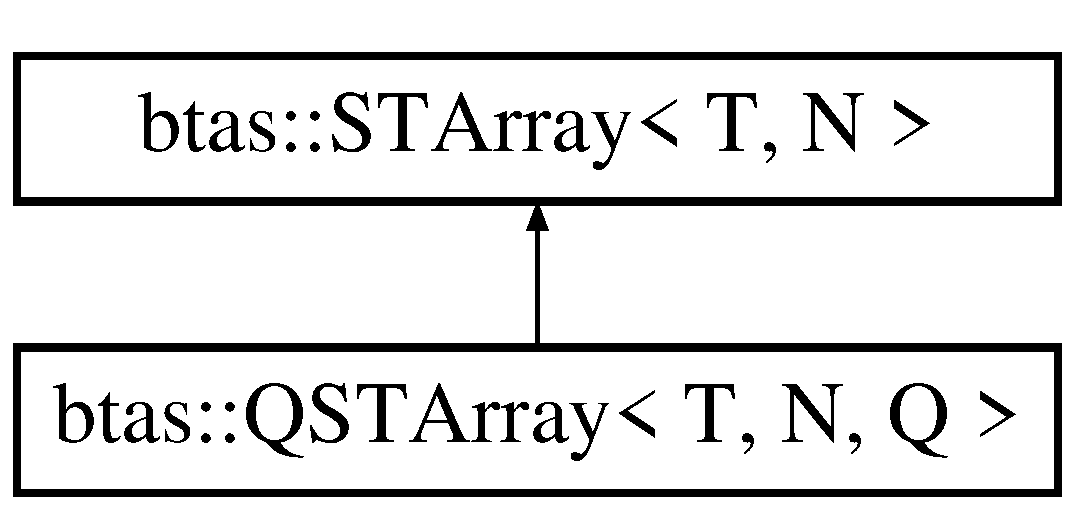
\includegraphics[height=2.000000cm]{db/dff/classbtas_1_1QSTArray}
\end{center}
\end{figure}
\subsection*{Public Types}
\begin{DoxyCompactItemize}
\item 
typedef {\bf S\-T\-Array}$<$ T, N $>$\\*
\-::{\bf const\-\_\-iterator} {\bf const\-\_\-iterator}
\item 
typedef {\bf S\-T\-Array}$<$ T, N $>$\-::{\bf iterator} {\bf iterator}
\end{DoxyCompactItemize}
\subsection*{Public Member Functions}
\begin{DoxyCompactItemize}
\item 
{\bf Q\-S\-T\-Array} ()
\begin{DoxyCompactList}\small\item\em Default constructor. \end{DoxyCompactList}\item 
{\bf $\sim$\-Q\-S\-T\-Array} ()
\begin{DoxyCompactList}\small\item\em Destructor. \end{DoxyCompactList}\item 
{\bf Q\-S\-T\-Array} (const Q \&q\-\_\-total, const {\bf T\-Vector}$<$ {\bf Qshapes}$<$ Q $>$, N $>$ \&q\-\_\-shape)
\begin{DoxyCompactList}\small\item\em Construct from quantum number indices. \end{DoxyCompactList}\item 
{\bf Q\-S\-T\-Array} (const Q \&q\-\_\-total, const {\bf T\-Vector}$<$ {\bf Qshapes}$<$ Q $>$, N $>$ \&q\-\_\-shape, const {\bf T\-Vector}$<$ {\bf Dshapes}, N $>$ \&d\-\_\-shape, bool \-\_\-allocate=true)
\begin{DoxyCompactList}\small\item\em Construct from quantum number indices and their dense shapes. \end{DoxyCompactList}\item 
{\bf Q\-S\-T\-Array} (const Q \&q\-\_\-total, const {\bf T\-Vector}$<$ {\bf Qshapes}$<$ Q $>$, N $>$ \&q\-\_\-shape, const {\bf T\-Vector}$<$ {\bf Dshapes}, N $>$ \&d\-\_\-shape, const T \&value)
\begin{DoxyCompactList}\small\item\em Construct from quantum number indices and their dense shapes and initialized by constant value. \end{DoxyCompactList}\item 
{\footnotesize template$<$class Generator $>$ }\\{\bf Q\-S\-T\-Array} (const Q \&q\-\_\-total, const {\bf T\-Vector}$<$ {\bf Qshapes}$<$ Q $>$, N $>$ \&q\-\_\-shape, const {\bf T\-Vector}$<$ {\bf Dshapes}, N $>$ \&d\-\_\-shape, Generator gen)
\begin{DoxyCompactList}\small\item\em Construct from quantum number indices and their dense shapes and initialized by gen() \end{DoxyCompactList}\item 
{\bf Q\-S\-T\-Array} (const {\bf Q\-S\-T\-Array} \&other)
\begin{DoxyCompactList}\small\item\em Copy constructor. \end{DoxyCompactList}\item 
{\bf Q\-S\-T\-Array} \& {\bf operator=} (const {\bf Q\-S\-T\-Array} \&other)
\begin{DoxyCompactList}\small\item\em Copy assignment operator. \end{DoxyCompactList}\item 
{\bf Q\-S\-T\-Array} ({\bf Q\-S\-T\-Array} \&\&other)
\begin{DoxyCompactList}\small\item\em Move constructor. \end{DoxyCompactList}\item 
{\bf Q\-S\-T\-Array} \& {\bf operator=} ({\bf Q\-S\-T\-Array} \&\&other)
\begin{DoxyCompactList}\small\item\em Move assignment operator. \end{DoxyCompactList}\item 
void {\bf reference} (const {\bf Q\-S\-T\-Array} \&other)
\begin{DoxyCompactList}\small\item\em make reference to other \end{DoxyCompactList}\item 
{\bf Q\-S\-T\-Array} {\bf subarray} (const {\bf T\-Vector}$<$ {\bf Dshapes}, N $>$ \&\-\_\-indxs) const 
\begin{DoxyCompactList}\small\item\em Make subarray reference. \end{DoxyCompactList}\item 
void {\bf resize} (const Q \&q\-\_\-total, const {\bf T\-Vector}$<$ {\bf Qshapes}$<$ Q $>$, N $>$ \&q\-\_\-shape)
\begin{DoxyCompactList}\small\item\em Construct from quantum number indices. \end{DoxyCompactList}\item 
void {\bf resize} (const Q \&q\-\_\-total, const {\bf T\-Vector}$<$ {\bf Qshapes}$<$ Q $>$, N $>$ \&q\-\_\-shape, const {\bf T\-Vector}$<$ {\bf Dshapes}, N $>$ \&d\-\_\-shape, bool \-\_\-allocate=true)
\begin{DoxyCompactList}\small\item\em Resize from quantum number indices and their dense shapes. \end{DoxyCompactList}\item 
void {\bf resize} (const Q \&q\-\_\-total, const {\bf T\-Vector}$<$ {\bf Qshapes}$<$ Q $>$, N $>$ \&q\-\_\-shape, const {\bf T\-Vector}$<$ {\bf Dshapes}, N $>$ \&d\-\_\-shape, const T \&value)
\begin{DoxyCompactList}\small\item\em Resize from quantum number indices and their dense shapes and initialized by constant value. \end{DoxyCompactList}\item 
{\footnotesize template$<$class Generator $>$ }\\void {\bf resize} (const Q \&q\-\_\-total, const {\bf T\-Vector}$<$ {\bf Qshapes}$<$ Q $>$, N $>$ \&q\-\_\-shape, const {\bf T\-Vector}$<$ {\bf Dshapes}, N $>$ \&d\-\_\-shape, Generator gen)
\begin{DoxyCompactList}\small\item\em Resize from quantum number indices and their dense shapes and initialized by gen() \end{DoxyCompactList}\item 
void {\bf operator=} (const T \&value)
\item 
void {\bf clear} ()
\begin{DoxyCompactList}\small\item\em Deallocation. \end{DoxyCompactList}\item 
void {\bf erase} (int \-\_\-rank, int \-\_\-index)
\begin{DoxyCompactList}\small\item\em Erase blocks of which have certain index. \end{DoxyCompactList}\item 
const Q \& {\bf q} () const 
\item 
const {\bf T\-Vector}$<$ {\bf Qshapes}$<$ Q $>$, N $>$ \& {\bf qshape} () const 
\item 
const {\bf Qshapes}$<$ Q $>$ \& {\bf qshape} (int i) const 
\item 
{\bf T\-Vector}$<$ Q, N $>$ {\bf qindex} (const {\bf I\-Vector}$<$ N $>$ \&block\-\_\-index) const 
\begin{DoxyCompactList}\small\item\em Returns quantum numbers corresponding to block-\/index. \end{DoxyCompactList}\item 
void {\bf parity} (const std\-::vector$<$ int $>$ \&p1)
\begin{DoxyCompactList}\small\item\em Inplaced parity operation. \end{DoxyCompactList}\item 
void {\bf parity} (const std\-::vector$<$ int $>$ \&p1, const std\-::vector$<$ int $>$ \&p2)
\begin{DoxyCompactList}\small\item\em Inplaced parity operation. \end{DoxyCompactList}\item 
{\bf Q\-S\-T\-Array} {\bf conjugate} () const 
\begin{DoxyCompactList}\small\item\em Returns conjugated referece. \end{DoxyCompactList}\item 
void {\bf conjugate\-\_\-self} ()
\begin{DoxyCompactList}\small\item\em Self conjugation. \end{DoxyCompactList}\end{DoxyCompactItemize}
\subsection*{Private Member Functions}
\begin{DoxyCompactItemize}
\item 
{\footnotesize template$<$class Archive $>$ }\\void {\bf serialize} (Archive \&ar, const unsigned int version)
\begin{DoxyCompactList}\small\item\em Boost serialization. \end{DoxyCompactList}\item 
bool {\bf mf\-\_\-check\-\_\-allowed} (const {\bf I\-Vector}$<$ N $>$ \&block\-\_\-index) const 
\begin{DoxyCompactList}\small\item\em Checking non-\/zero block. \end{DoxyCompactList}\end{DoxyCompactItemize}
\subsection*{Private Attributes}
\begin{DoxyCompactItemize}
\item 
Q {\bf m\-\_\-q\-\_\-total}
\begin{DoxyCompactList}\small\item\em Total quantum number of array. \end{DoxyCompactList}\item 
{\bf T\-Vector}$<$ {\bf Qshapes}$<$ Q $>$, N $>$ {\bf m\-\_\-q\-\_\-shape}
\begin{DoxyCompactList}\small\item\em \doxyref{Quantum}{p.}{d8/df8/classQuantum} number indices. \end{DoxyCompactList}\end{DoxyCompactItemize}
\subsection*{Friends}
\begin{DoxyCompactItemize}
\item 
class {\bf boost\-::serialization\-::access}
\end{DoxyCompactItemize}
\subsection*{Additional Inherited Members}


\subsection{Detailed Description}
\subsubsection*{template$<$typename T, size\-\_\-t N, class Q = Quantum$>$class btas\-::\-Q\-S\-T\-Array$<$ T, N, Q $>$}

\doxyref{Quantum}{p.}{d8/df8/classQuantum} number-\/based block sparse array. 

Definition at line 17 of file Q\-S\-T\-Array.\-h.



\subsection{Member Typedef Documentation}
\index{btas\-::\-Q\-S\-T\-Array@{btas\-::\-Q\-S\-T\-Array}!const\-\_\-iterator@{const\-\_\-iterator}}
\index{const\-\_\-iterator@{const\-\_\-iterator}!btas::QSTArray@{btas\-::\-Q\-S\-T\-Array}}
\subsubsection[{const\-\_\-iterator}]{\setlength{\rightskip}{0pt plus 5cm}template$<$typename T, size\-\_\-t N, class Q = Quantum$>$ typedef {\bf S\-T\-Array}$<$T, N$>$\-::{\bf const\-\_\-iterator} {\bf btas\-::\-Q\-S\-T\-Array}$<$ T, N, Q $>$\-::{\bf const\-\_\-iterator}}\label{db/dff/classbtas_1_1QSTArray_a30c5f29d49ee894681e94aa6fa7cad59}


Definition at line 19 of file Q\-S\-T\-Array.\-h.

\index{btas\-::\-Q\-S\-T\-Array@{btas\-::\-Q\-S\-T\-Array}!iterator@{iterator}}
\index{iterator@{iterator}!btas::QSTArray@{btas\-::\-Q\-S\-T\-Array}}
\subsubsection[{iterator}]{\setlength{\rightskip}{0pt plus 5cm}template$<$typename T, size\-\_\-t N, class Q = Quantum$>$ typedef {\bf S\-T\-Array}$<$T, N$>$\-::{\bf iterator} {\bf btas\-::\-Q\-S\-T\-Array}$<$ T, N, Q $>$\-::{\bf iterator}}\label{db/dff/classbtas_1_1QSTArray_a3b60ccbe20f3bbd0df90f82198b39d8d}


Definition at line 20 of file Q\-S\-T\-Array.\-h.



\subsection{Constructor \& Destructor Documentation}
\index{btas\-::\-Q\-S\-T\-Array@{btas\-::\-Q\-S\-T\-Array}!Q\-S\-T\-Array@{Q\-S\-T\-Array}}
\index{Q\-S\-T\-Array@{Q\-S\-T\-Array}!btas::QSTArray@{btas\-::\-Q\-S\-T\-Array}}
\subsubsection[{Q\-S\-T\-Array}]{\setlength{\rightskip}{0pt plus 5cm}template$<$typename T, size\-\_\-t N, class Q = Quantum$>$ {\bf btas\-::\-Q\-S\-T\-Array}$<$ T, N, Q $>$\-::{\bf Q\-S\-T\-Array} (
\begin{DoxyParamCaption}
{}
\end{DoxyParamCaption}
)\hspace{0.3cm}{\ttfamily [inline]}}\label{db/dff/classbtas_1_1QSTArray_abbca8fbe508c1fefd2c1ba33d815ee94}


Default constructor. 



Definition at line 44 of file Q\-S\-T\-Array.\-h.

\index{btas\-::\-Q\-S\-T\-Array@{btas\-::\-Q\-S\-T\-Array}!$\sim$\-Q\-S\-T\-Array@{$\sim$\-Q\-S\-T\-Array}}
\index{$\sim$\-Q\-S\-T\-Array@{$\sim$\-Q\-S\-T\-Array}!btas::QSTArray@{btas\-::\-Q\-S\-T\-Array}}
\subsubsection[{$\sim$\-Q\-S\-T\-Array}]{\setlength{\rightskip}{0pt plus 5cm}template$<$typename T, size\-\_\-t N, class Q = Quantum$>$ {\bf btas\-::\-Q\-S\-T\-Array}$<$ T, N, Q $>$\-::$\sim${\bf Q\-S\-T\-Array} (
\begin{DoxyParamCaption}
{}
\end{DoxyParamCaption}
)\hspace{0.3cm}{\ttfamily [inline]}}\label{db/dff/classbtas_1_1QSTArray_aef76b553ff90f83d3b0b0773ab9bd601}


Destructor. 



Definition at line 47 of file Q\-S\-T\-Array.\-h.

\index{btas\-::\-Q\-S\-T\-Array@{btas\-::\-Q\-S\-T\-Array}!Q\-S\-T\-Array@{Q\-S\-T\-Array}}
\index{Q\-S\-T\-Array@{Q\-S\-T\-Array}!btas::QSTArray@{btas\-::\-Q\-S\-T\-Array}}
\subsubsection[{Q\-S\-T\-Array}]{\setlength{\rightskip}{0pt plus 5cm}template$<$typename T, size\-\_\-t N, class Q = Quantum$>$ {\bf btas\-::\-Q\-S\-T\-Array}$<$ T, N, Q $>$\-::{\bf Q\-S\-T\-Array} (
\begin{DoxyParamCaption}
\item[{const Q \&}]{q\-\_\-total, }
\item[{const {\bf T\-Vector}$<$ {\bf Qshapes}$<$ Q $>$, N $>$ \&}]{q\-\_\-shape}
\end{DoxyParamCaption}
)\hspace{0.3cm}{\ttfamily [inline]}}\label{db/dff/classbtas_1_1QSTArray_aa4322694050adf875ba762508afdcb5d}


Construct from quantum number indices. 



Definition at line 51 of file Q\-S\-T\-Array.\-h.



References btas\-::\-Q\-S\-T\-Array$<$ T, N, Q $>$\-::resize().

\index{btas\-::\-Q\-S\-T\-Array@{btas\-::\-Q\-S\-T\-Array}!Q\-S\-T\-Array@{Q\-S\-T\-Array}}
\index{Q\-S\-T\-Array@{Q\-S\-T\-Array}!btas::QSTArray@{btas\-::\-Q\-S\-T\-Array}}
\subsubsection[{Q\-S\-T\-Array}]{\setlength{\rightskip}{0pt plus 5cm}template$<$typename T, size\-\_\-t N, class Q = Quantum$>$ {\bf btas\-::\-Q\-S\-T\-Array}$<$ T, N, Q $>$\-::{\bf Q\-S\-T\-Array} (
\begin{DoxyParamCaption}
\item[{const Q \&}]{q\-\_\-total, }
\item[{const {\bf T\-Vector}$<$ {\bf Qshapes}$<$ Q $>$, N $>$ \&}]{q\-\_\-shape, }
\item[{const {\bf T\-Vector}$<$ {\bf Dshapes}, N $>$ \&}]{d\-\_\-shape, }
\item[{bool}]{\-\_\-allocate = {\ttfamily true}}
\end{DoxyParamCaption}
)\hspace{0.3cm}{\ttfamily [inline]}}\label{db/dff/classbtas_1_1QSTArray_a4066191f6c9d1170aaa1645793bd7318}


Construct from quantum number indices and their dense shapes. 



Definition at line 56 of file Q\-S\-T\-Array.\-h.



References btas\-::\-Q\-S\-T\-Array$<$ T, N, Q $>$\-::resize().

\index{btas\-::\-Q\-S\-T\-Array@{btas\-::\-Q\-S\-T\-Array}!Q\-S\-T\-Array@{Q\-S\-T\-Array}}
\index{Q\-S\-T\-Array@{Q\-S\-T\-Array}!btas::QSTArray@{btas\-::\-Q\-S\-T\-Array}}
\subsubsection[{Q\-S\-T\-Array}]{\setlength{\rightskip}{0pt plus 5cm}template$<$typename T, size\-\_\-t N, class Q = Quantum$>$ {\bf btas\-::\-Q\-S\-T\-Array}$<$ T, N, Q $>$\-::{\bf Q\-S\-T\-Array} (
\begin{DoxyParamCaption}
\item[{const Q \&}]{q\-\_\-total, }
\item[{const {\bf T\-Vector}$<$ {\bf Qshapes}$<$ Q $>$, N $>$ \&}]{q\-\_\-shape, }
\item[{const {\bf T\-Vector}$<$ {\bf Dshapes}, N $>$ \&}]{d\-\_\-shape, }
\item[{const T \&}]{value}
\end{DoxyParamCaption}
)\hspace{0.3cm}{\ttfamily [inline]}}\label{db/dff/classbtas_1_1QSTArray_ae8b903926e290ae796797fe82ecb06c2}


Construct from quantum number indices and their dense shapes and initialized by constant value. 



Definition at line 61 of file Q\-S\-T\-Array.\-h.



References btas\-::\-Q\-S\-T\-Array$<$ T, N, Q $>$\-::resize().

\index{btas\-::\-Q\-S\-T\-Array@{btas\-::\-Q\-S\-T\-Array}!Q\-S\-T\-Array@{Q\-S\-T\-Array}}
\index{Q\-S\-T\-Array@{Q\-S\-T\-Array}!btas::QSTArray@{btas\-::\-Q\-S\-T\-Array}}
\subsubsection[{Q\-S\-T\-Array}]{\setlength{\rightskip}{0pt plus 5cm}template$<$typename T, size\-\_\-t N, class Q = Quantum$>$ template$<$class Generator $>$ {\bf btas\-::\-Q\-S\-T\-Array}$<$ T, N, Q $>$\-::{\bf Q\-S\-T\-Array} (
\begin{DoxyParamCaption}
\item[{const Q \&}]{q\-\_\-total, }
\item[{const {\bf T\-Vector}$<$ {\bf Qshapes}$<$ Q $>$, N $>$ \&}]{q\-\_\-shape, }
\item[{const {\bf T\-Vector}$<$ {\bf Dshapes}, N $>$ \&}]{d\-\_\-shape, }
\item[{Generator}]{gen}
\end{DoxyParamCaption}
)\hspace{0.3cm}{\ttfamily [inline]}}\label{db/dff/classbtas_1_1QSTArray_a3367e0a6a4c8dbc82536b66d0ba47ae8}


Construct from quantum number indices and their dense shapes and initialized by gen() 



Definition at line 67 of file Q\-S\-T\-Array.\-h.



References btas\-::\-Q\-S\-T\-Array$<$ T, N, Q $>$\-::resize().

\index{btas\-::\-Q\-S\-T\-Array@{btas\-::\-Q\-S\-T\-Array}!Q\-S\-T\-Array@{Q\-S\-T\-Array}}
\index{Q\-S\-T\-Array@{Q\-S\-T\-Array}!btas::QSTArray@{btas\-::\-Q\-S\-T\-Array}}
\subsubsection[{Q\-S\-T\-Array}]{\setlength{\rightskip}{0pt plus 5cm}template$<$typename T, size\-\_\-t N, class Q = Quantum$>$ {\bf btas\-::\-Q\-S\-T\-Array}$<$ T, N, Q $>$\-::{\bf Q\-S\-T\-Array} (
\begin{DoxyParamCaption}
\item[{const {\bf Q\-S\-T\-Array}$<$ T, N, Q $>$ \&}]{other}
\end{DoxyParamCaption}
)\hspace{0.3cm}{\ttfamily [inline]}}\label{db/dff/classbtas_1_1QSTArray_aa73335d16ac4090b2c7e49723caed75e}


Copy constructor. 



Definition at line 76 of file Q\-S\-T\-Array.\-h.



References btas\-::\-Q\-S\-T\-Array$<$ T, N, Q $>$\-::m\-\_\-q\-\_\-shape, and btas\-::\-Q\-S\-T\-Array$<$ T, N, Q $>$\-::m\-\_\-q\-\_\-total.

\index{btas\-::\-Q\-S\-T\-Array@{btas\-::\-Q\-S\-T\-Array}!Q\-S\-T\-Array@{Q\-S\-T\-Array}}
\index{Q\-S\-T\-Array@{Q\-S\-T\-Array}!btas::QSTArray@{btas\-::\-Q\-S\-T\-Array}}
\subsubsection[{Q\-S\-T\-Array}]{\setlength{\rightskip}{0pt plus 5cm}template$<$typename T, size\-\_\-t N, class Q = Quantum$>$ {\bf btas\-::\-Q\-S\-T\-Array}$<$ T, N, Q $>$\-::{\bf Q\-S\-T\-Array} (
\begin{DoxyParamCaption}
\item[{{\bf Q\-S\-T\-Array}$<$ T, N, Q $>$ \&\&}]{other}
\end{DoxyParamCaption}
)\hspace{0.3cm}{\ttfamily [inline]}}\label{db/dff/classbtas_1_1QSTArray_aa15a78dfac6c23748124374d5ef44d5a}


Move constructor. 



Definition at line 94 of file Q\-S\-T\-Array.\-h.



References btas\-::\-Q\-S\-T\-Array$<$ T, N, Q $>$\-::m\-\_\-q\-\_\-shape, and btas\-::\-Q\-S\-T\-Array$<$ T, N, Q $>$\-::m\-\_\-q\-\_\-total.



\subsection{Member Function Documentation}
\index{btas\-::\-Q\-S\-T\-Array@{btas\-::\-Q\-S\-T\-Array}!clear@{clear}}
\index{clear@{clear}!btas::QSTArray@{btas\-::\-Q\-S\-T\-Array}}
\subsubsection[{clear}]{\setlength{\rightskip}{0pt plus 5cm}template$<$typename T, size\-\_\-t N, class Q = Quantum$>$ void {\bf btas\-::\-Q\-S\-T\-Array}$<$ T, N, Q $>$\-::clear (
\begin{DoxyParamCaption}
{}
\end{DoxyParamCaption}
)\hspace{0.3cm}{\ttfamily [inline]}, {\ttfamily [virtual]}}\label{db/dff/classbtas_1_1QSTArray_a571c148e5351fbac6db7ca00e8cadb79}


Deallocation. 



Reimplemented from {\bf btas\-::\-S\-T\-Array$<$ T, N $>$} \doxyref{}{p.}{d7/d05/classbtas_1_1STArray_a571a8d5d37e0a90a1e175c2fb305c388}.



Definition at line 205 of file Q\-S\-T\-Array.\-h.



References btas\-::\-S\-T\-Array$<$ T, N $>$\-::clear(), btas\-::\-Q\-S\-T\-Array$<$ T, N, Q $>$\-::m\-\_\-q\-\_\-shape, and btas\-::\-Q\-S\-T\-Array$<$ T, N, Q $>$\-::m\-\_\-q\-\_\-total.



Referenced by mps\-::add(), mps\-::compress(), mps\-::dot(), mps\-::gemm(), mps\-::gemv(), mps\-::inprod(), btas\-::\-Q\-S\-Dgesvd(), and S\-E\-R\-I\-A\-L\-I\-Z\-E\-\_\-\-T\-E\-S\-T().

\index{btas\-::\-Q\-S\-T\-Array@{btas\-::\-Q\-S\-T\-Array}!conjugate@{conjugate}}
\index{conjugate@{conjugate}!btas::QSTArray@{btas\-::\-Q\-S\-T\-Array}}
\subsubsection[{conjugate}]{\setlength{\rightskip}{0pt plus 5cm}template$<$typename T, size\-\_\-t N, class Q = Quantum$>$ {\bf Q\-S\-T\-Array} {\bf btas\-::\-Q\-S\-T\-Array}$<$ T, N, Q $>$\-::conjugate (
\begin{DoxyParamCaption}
{}
\end{DoxyParamCaption}
) const\hspace{0.3cm}{\ttfamily [inline]}}\label{db/dff/classbtas_1_1QSTArray_af82a3e1c9e2d35451d144af7e1f04d67}


Returns conjugated referece. 

Conjugation means flipping direction of quantum indices. 

Definition at line 288 of file Q\-S\-T\-Array.\-h.



References btas\-::\-Q\-S\-T\-Array$<$ T, N, Q $>$\-::m\-\_\-q\-\_\-shape, and btas\-::\-Q\-S\-T\-Array$<$ T, N, Q $>$\-::m\-\_\-q\-\_\-total.



Referenced by Q\-S\-P\-A\-R\-S\-E\-\_\-\-T\-E\-S\-T().

\index{btas\-::\-Q\-S\-T\-Array@{btas\-::\-Q\-S\-T\-Array}!conjugate\-\_\-self@{conjugate\-\_\-self}}
\index{conjugate\-\_\-self@{conjugate\-\_\-self}!btas::QSTArray@{btas\-::\-Q\-S\-T\-Array}}
\subsubsection[{conjugate\-\_\-self}]{\setlength{\rightskip}{0pt plus 5cm}template$<$typename T, size\-\_\-t N, class Q = Quantum$>$ void {\bf btas\-::\-Q\-S\-T\-Array}$<$ T, N, Q $>$\-::conjugate\-\_\-self (
\begin{DoxyParamCaption}
{}
\end{DoxyParamCaption}
)\hspace{0.3cm}{\ttfamily [inline]}}\label{db/dff/classbtas_1_1QSTArray_a58deaeddc551f2f91a67a625703dc2d2}


Self conjugation. 



Definition at line 298 of file Q\-S\-T\-Array.\-h.



References btas\-::\-Q\-S\-T\-Array$<$ T, N, Q $>$\-::m\-\_\-q\-\_\-shape, and btas\-::\-Q\-S\-T\-Array$<$ T, N, Q $>$\-::m\-\_\-q\-\_\-total.

\index{btas\-::\-Q\-S\-T\-Array@{btas\-::\-Q\-S\-T\-Array}!erase@{erase}}
\index{erase@{erase}!btas::QSTArray@{btas\-::\-Q\-S\-T\-Array}}
\subsubsection[{erase}]{\setlength{\rightskip}{0pt plus 5cm}template$<$typename T, size\-\_\-t N, class Q = Quantum$>$ void {\bf btas\-::\-Q\-S\-T\-Array}$<$ T, N, Q $>$\-::erase (
\begin{DoxyParamCaption}
\item[{int}]{\-\_\-rank, }
\item[{int}]{\-\_\-index}
\end{DoxyParamCaption}
)\hspace{0.3cm}{\ttfamily [inline]}, {\ttfamily [virtual]}}\label{db/dff/classbtas_1_1QSTArray_a327328c903afc8c91d86fb6f7e6254c0}


Erase blocks of which have certain index. 

Not good design, since it can't check quantum numbers 
\begin{DoxyParams}{Parameters}
{\em \-\_\-rank} & rank in which index is associated \\
\hline
{\em \-\_\-index} & index to be removed \\
\hline
\end{DoxyParams}


Reimplemented from {\bf btas\-::\-S\-T\-Array$<$ T, N $>$} \doxyref{}{p.}{d7/d05/classbtas_1_1STArray_a7333d1b7dc605229848b55940a0f9d8e}.



Definition at line 216 of file Q\-S\-T\-Array.\-h.



References btas\-::\-S\-T\-Array$<$ T, N $>$\-::begin(), btas\-::\-S\-T\-Array$<$ T, N $>$\-::erase(), and btas\-::\-Q\-S\-T\-Array$<$ T, N, Q $>$\-::m\-\_\-q\-\_\-shape.



Referenced by Q\-S\-P\-A\-R\-S\-E\-\_\-\-T\-E\-S\-T().

\index{btas\-::\-Q\-S\-T\-Array@{btas\-::\-Q\-S\-T\-Array}!mf\-\_\-check\-\_\-allowed@{mf\-\_\-check\-\_\-allowed}}
\index{mf\-\_\-check\-\_\-allowed@{mf\-\_\-check\-\_\-allowed}!btas::QSTArray@{btas\-::\-Q\-S\-T\-Array}}
\subsubsection[{mf\-\_\-check\-\_\-allowed}]{\setlength{\rightskip}{0pt plus 5cm}template$<$typename T, size\-\_\-t N, class Q = Quantum$>$ bool {\bf btas\-::\-Q\-S\-T\-Array}$<$ T, N, Q $>$\-::mf\-\_\-check\-\_\-allowed (
\begin{DoxyParamCaption}
\item[{const {\bf I\-Vector}$<$ N $>$ \&}]{block\-\_\-index}
\end{DoxyParamCaption}
) const\hspace{0.3cm}{\ttfamily [inline]}, {\ttfamily [private]}, {\ttfamily [virtual]}}\label{db/dff/classbtas_1_1QSTArray_abe907fce0f2895ac85829557128537f1}


Checking non-\/zero block. 

\doxyref{S\-T\-Array$<$\-T, N$>$\-::mf\-\_\-check\-\_\-allowed}{p.}{d7/d05/classbtas_1_1STArray_a5cbdb42d66a0b2d00e8d9e42476ba4fb} is overridden here 

Reimplemented from {\bf btas\-::\-S\-T\-Array$<$ T, N $>$} \doxyref{}{p.}{d7/d05/classbtas_1_1STArray_a5cbdb42d66a0b2d00e8d9e42476ba4fb}.



Definition at line 33 of file Q\-S\-T\-Array.\-h.



References btas\-::\-Q\-S\-T\-Array$<$ T, N, Q $>$\-::m\-\_\-q\-\_\-shape, and btas\-::\-Q\-S\-T\-Array$<$ T, N, Q $>$\-::m\-\_\-q\-\_\-total.

\index{btas\-::\-Q\-S\-T\-Array@{btas\-::\-Q\-S\-T\-Array}!operator=@{operator=}}
\index{operator=@{operator=}!btas::QSTArray@{btas\-::\-Q\-S\-T\-Array}}
\subsubsection[{operator=}]{\setlength{\rightskip}{0pt plus 5cm}template$<$typename T, size\-\_\-t N, class Q = Quantum$>$ {\bf Q\-S\-T\-Array}\& {\bf btas\-::\-Q\-S\-T\-Array}$<$ T, N, Q $>$\-::operator= (
\begin{DoxyParamCaption}
\item[{const {\bf Q\-S\-T\-Array}$<$ T, N, Q $>$ \&}]{other}
\end{DoxyParamCaption}
)\hspace{0.3cm}{\ttfamily [inline]}}\label{db/dff/classbtas_1_1QSTArray_a4ef711e62b42dd53ef541fbe95e18aef}


Copy assignment operator. 



Definition at line 82 of file Q\-S\-T\-Array.\-h.



References btas\-::\-S\-T\-Array$<$ T, N $>$\-::copy(), btas\-::\-Q\-S\-T\-Array$<$ T, N, Q $>$\-::m\-\_\-q\-\_\-shape, and btas\-::\-Q\-S\-T\-Array$<$ T, N, Q $>$\-::m\-\_\-q\-\_\-total.

\index{btas\-::\-Q\-S\-T\-Array@{btas\-::\-Q\-S\-T\-Array}!operator=@{operator=}}
\index{operator=@{operator=}!btas::QSTArray@{btas\-::\-Q\-S\-T\-Array}}
\subsubsection[{operator=}]{\setlength{\rightskip}{0pt plus 5cm}template$<$typename T, size\-\_\-t N, class Q = Quantum$>$ {\bf Q\-S\-T\-Array}\& {\bf btas\-::\-Q\-S\-T\-Array}$<$ T, N, Q $>$\-::operator= (
\begin{DoxyParamCaption}
\item[{{\bf Q\-S\-T\-Array}$<$ T, N, Q $>$ \&\&}]{other}
\end{DoxyParamCaption}
)\hspace{0.3cm}{\ttfamily [inline]}}\label{db/dff/classbtas_1_1QSTArray_a0e6fcafa6efc89c866f9c47f80920882}


Move assignment operator. 



Definition at line 100 of file Q\-S\-T\-Array.\-h.



References btas\-::\-Q\-S\-T\-Array$<$ T, N, Q $>$\-::m\-\_\-q\-\_\-shape, btas\-::\-Q\-S\-T\-Array$<$ T, N, Q $>$\-::m\-\_\-q\-\_\-total, and btas\-::\-S\-T\-Array$<$ T, N $>$\-::operator=().

\index{btas\-::\-Q\-S\-T\-Array@{btas\-::\-Q\-S\-T\-Array}!operator=@{operator=}}
\index{operator=@{operator=}!btas::QSTArray@{btas\-::\-Q\-S\-T\-Array}}
\subsubsection[{operator=}]{\setlength{\rightskip}{0pt plus 5cm}template$<$typename T, size\-\_\-t N, class Q = Quantum$>$ void {\bf btas\-::\-Q\-S\-T\-Array}$<$ T, N, Q $>$\-::operator= (
\begin{DoxyParamCaption}
\item[{const T \&}]{value}
\end{DoxyParamCaption}
)\hspace{0.3cm}{\ttfamily [inline]}}\label{db/dff/classbtas_1_1QSTArray_a02417ba100f5f9273eccb0d663f07ddb}


Definition at line 195 of file Q\-S\-T\-Array.\-h.



References btas\-::\-S\-T\-Array$<$ T, N $>$\-::operator=().

\index{btas\-::\-Q\-S\-T\-Array@{btas\-::\-Q\-S\-T\-Array}!parity@{parity}}
\index{parity@{parity}!btas::QSTArray@{btas\-::\-Q\-S\-T\-Array}}
\subsubsection[{parity}]{\setlength{\rightskip}{0pt plus 5cm}template$<$typename T, size\-\_\-t N, class Q = Quantum$>$ void {\bf btas\-::\-Q\-S\-T\-Array}$<$ T, N, Q $>$\-::parity (
\begin{DoxyParamCaption}
\item[{const std\-::vector$<$ int $>$ \&}]{p1}
\end{DoxyParamCaption}
)\hspace{0.3cm}{\ttfamily [inline]}}\label{db/dff/classbtas_1_1QSTArray_adc5827fc2e593b94b375fc186144e0e0}


Inplaced parity operation. 

For each non-\/zero block, if q = sum\-\_\-\{i\} m\-\_\-q\-\_\-shape[p1[i]] has odd particle number, scale -\/1 

Definition at line 258 of file Q\-S\-T\-Array.\-h.



References btas\-::\-S\-T\-Array$<$ T, N $>$\-::begin(), btas\-::\-S\-T\-Array$<$ T, N $>$\-::end(), btas\-::\-S\-T\-Array$<$ T, N $>$\-::index(), and btas\-::\-Q\-S\-T\-Array$<$ T, N, Q $>$\-::m\-\_\-q\-\_\-shape.



Referenced by btas\-::\-Q\-S\-T\-Array$<$ T, N, Q $>$\-::parity().

\index{btas\-::\-Q\-S\-T\-Array@{btas\-::\-Q\-S\-T\-Array}!parity@{parity}}
\index{parity@{parity}!btas::QSTArray@{btas\-::\-Q\-S\-T\-Array}}
\subsubsection[{parity}]{\setlength{\rightskip}{0pt plus 5cm}template$<$typename T, size\-\_\-t N, class Q = Quantum$>$ void {\bf btas\-::\-Q\-S\-T\-Array}$<$ T, N, Q $>$\-::parity (
\begin{DoxyParamCaption}
\item[{const std\-::vector$<$ int $>$ \&}]{p1, }
\item[{const std\-::vector$<$ int $>$ \&}]{p2}
\end{DoxyParamCaption}
)\hspace{0.3cm}{\ttfamily [inline]}}\label{db/dff/classbtas_1_1QSTArray_a81bfbc024c8bfdeb3e6862ef00210307}


Inplaced parity operation. 

For each non-\/zero block, scale by sign = prod\-\_\-\{i\} ( -\/1 \-: both m\-\_\-q\-\_\-shape[p1[i]] and m\-\_\-q\-\_\-shape[p2[i]] have odd particle number ) 

Definition at line 273 of file Q\-S\-T\-Array.\-h.



References btas\-::\-S\-T\-Array$<$ T, N $>$\-::begin(), btas\-::\-S\-T\-Array$<$ T, N $>$\-::end(), btas\-::\-S\-T\-Array$<$ T, N $>$\-::index(), btas\-::\-Q\-S\-T\-Array$<$ T, N, Q $>$\-::m\-\_\-q\-\_\-shape, and btas\-::\-Q\-S\-T\-Array$<$ T, N, Q $>$\-::parity().

\index{btas\-::\-Q\-S\-T\-Array@{btas\-::\-Q\-S\-T\-Array}!q@{q}}
\index{q@{q}!btas::QSTArray@{btas\-::\-Q\-S\-T\-Array}}
\subsubsection[{q}]{\setlength{\rightskip}{0pt plus 5cm}template$<$typename T, size\-\_\-t N, class Q = Quantum$>$ const Q\& {\bf btas\-::\-Q\-S\-T\-Array}$<$ T, N, Q $>$\-::q (
\begin{DoxyParamCaption}
{}
\end{DoxyParamCaption}
) const\hspace{0.3cm}{\ttfamily [inline]}}\label{db/dff/classbtas_1_1QSTArray_a92843c5f7a1edb28a19580e2564e956f}
! Erase blocks of which have certain set of indices $\ast$! 

Definition at line 243 of file Q\-S\-T\-Array.\-h.



References btas\-::\-Q\-S\-T\-Array$<$ T, N, Q $>$\-::m\-\_\-q\-\_\-total.



Referenced by btas\-::\-Q\-S\-Daxpy(), btas\-::\-Q\-S\-Dcopy(), btas\-::\-Q\-S\-Ddotc(), btas\-::\-Q\-S\-Ddotu(), btas\-::\-Q\-S\-Dgemm(), btas\-::\-Q\-S\-Dgemv(), btas\-::\-Q\-S\-Dger(), btas\-::\-Q\-S\-Dgesvd(), btas\-::\-Q\-S\-Dpermute(), btas\-::\-Q\-S\-Tdsum(), btas\-::\-Q\-S\-Texpand(), and btas\-::\-Q\-S\-Tmerge().

\index{btas\-::\-Q\-S\-T\-Array@{btas\-::\-Q\-S\-T\-Array}!qindex@{qindex}}
\index{qindex@{qindex}!btas::QSTArray@{btas\-::\-Q\-S\-T\-Array}}
\subsubsection[{qindex}]{\setlength{\rightskip}{0pt plus 5cm}template$<$typename T, size\-\_\-t N, class Q = Quantum$>$ {\bf T\-Vector}$<$Q, N$>$ {\bf btas\-::\-Q\-S\-T\-Array}$<$ T, N, Q $>$\-::qindex (
\begin{DoxyParamCaption}
\item[{const {\bf I\-Vector}$<$ N $>$ \&}]{block\-\_\-index}
\end{DoxyParamCaption}
) const\hspace{0.3cm}{\ttfamily [inline]}}\label{db/dff/classbtas_1_1QSTArray_a07ebb34d17d64bacf799123275fdbcb4}


Returns quantum numbers corresponding to block-\/index. 



Definition at line 248 of file Q\-S\-T\-Array.\-h.



References btas\-::\-Q\-S\-T\-Array$<$ T, N, Q $>$\-::m\-\_\-q\-\_\-shape.

\index{btas\-::\-Q\-S\-T\-Array@{btas\-::\-Q\-S\-T\-Array}!qshape@{qshape}}
\index{qshape@{qshape}!btas::QSTArray@{btas\-::\-Q\-S\-T\-Array}}
\subsubsection[{qshape}]{\setlength{\rightskip}{0pt plus 5cm}template$<$typename T, size\-\_\-t N, class Q = Quantum$>$ const {\bf T\-Vector}$<${\bf Qshapes}$<$Q$>$, N$>$\& {\bf btas\-::\-Q\-S\-T\-Array}$<$ T, N, Q $>$\-::qshape (
\begin{DoxyParamCaption}
{}
\end{DoxyParamCaption}
) const\hspace{0.3cm}{\ttfamily [inline]}}\label{db/dff/classbtas_1_1QSTArray_a44c76f1ce6f764450b81952a7249844c}


Definition at line 244 of file Q\-S\-T\-Array.\-h.



References btas\-::\-Q\-S\-T\-Array$<$ T, N, Q $>$\-::m\-\_\-q\-\_\-shape.



Referenced by mps\-::add(), mps\-::gemm(), mps\-::gemv(), mps\-::inprod(), btas\-::\-Q\-S\-Daxpy(), btas\-::\-Q\-S\-Dcopy(), btas\-::\-Q\-S\-Ddotc(), btas\-::\-Q\-S\-Ddotu(), btas\-::\-Q\-S\-Dgemm(), btas\-::\-Q\-S\-Dgemv(), btas\-::\-Q\-S\-Dger(), btas\-::\-Q\-S\-Dgesvd(), btas\-::\-Q\-S\-Dpermute(), Q\-S\-P\-A\-R\-S\-E\-\_\-\-T\-E\-S\-T(), btas\-::\-Q\-S\-Tdsum(), btas\-::\-Q\-S\-Texpand(), and btas\-::\-Q\-S\-Tmerge().

\index{btas\-::\-Q\-S\-T\-Array@{btas\-::\-Q\-S\-T\-Array}!qshape@{qshape}}
\index{qshape@{qshape}!btas::QSTArray@{btas\-::\-Q\-S\-T\-Array}}
\subsubsection[{qshape}]{\setlength{\rightskip}{0pt plus 5cm}template$<$typename T, size\-\_\-t N, class Q = Quantum$>$ const {\bf Qshapes}$<$Q$>$\& {\bf btas\-::\-Q\-S\-T\-Array}$<$ T, N, Q $>$\-::qshape (
\begin{DoxyParamCaption}
\item[{int}]{i}
\end{DoxyParamCaption}
) const\hspace{0.3cm}{\ttfamily [inline]}}\label{db/dff/classbtas_1_1QSTArray_aab8e0927f3722f4e68621dfd77eaec2c}


Definition at line 245 of file Q\-S\-T\-Array.\-h.



References btas\-::\-Q\-S\-T\-Array$<$ T, N, Q $>$\-::m\-\_\-q\-\_\-shape.

\index{btas\-::\-Q\-S\-T\-Array@{btas\-::\-Q\-S\-T\-Array}!reference@{reference}}
\index{reference@{reference}!btas::QSTArray@{btas\-::\-Q\-S\-T\-Array}}
\subsubsection[{reference}]{\setlength{\rightskip}{0pt plus 5cm}template$<$typename T, size\-\_\-t N, class Q = Quantum$>$ void {\bf btas\-::\-Q\-S\-T\-Array}$<$ T, N, Q $>$\-::reference (
\begin{DoxyParamCaption}
\item[{const {\bf Q\-S\-T\-Array}$<$ T, N, Q $>$ \&}]{other}
\end{DoxyParamCaption}
)\hspace{0.3cm}{\ttfamily [inline]}}\label{db/dff/classbtas_1_1QSTArray_aafb2d4a91237ef7b42b739ce1cefdbac}


make reference to other 

not complete reference, since elements in m\-\_\-store are only shared. so, even if m\-\_\-shape or m\-\_\-stride is changed, it won't be affected. 

Definition at line 111 of file Q\-S\-T\-Array.\-h.



References btas\-::\-Q\-S\-T\-Array$<$ T, N, Q $>$\-::m\-\_\-q\-\_\-shape, btas\-::\-Q\-S\-T\-Array$<$ T, N, Q $>$\-::m\-\_\-q\-\_\-total, and btas\-::\-S\-T\-Array$<$ T, N $>$\-::reference().



Referenced by btas\-::\-Q\-S\-Dcontract().

\index{btas\-::\-Q\-S\-T\-Array@{btas\-::\-Q\-S\-T\-Array}!resize@{resize}}
\index{resize@{resize}!btas::QSTArray@{btas\-::\-Q\-S\-T\-Array}}
\subsubsection[{resize}]{\setlength{\rightskip}{0pt plus 5cm}template$<$typename T, size\-\_\-t N, class Q = Quantum$>$ void {\bf btas\-::\-Q\-S\-T\-Array}$<$ T, N, Q $>$\-::resize (
\begin{DoxyParamCaption}
\item[{const Q \&}]{q\-\_\-total, }
\item[{const {\bf T\-Vector}$<$ {\bf Qshapes}$<$ Q $>$, N $>$ \&}]{q\-\_\-shape}
\end{DoxyParamCaption}
)\hspace{0.3cm}{\ttfamily [inline]}}\label{db/dff/classbtas_1_1QSTArray_ab1d8733d0c7e9ac623f1e7a43987bf59}


Construct from quantum number indices. 



Definition at line 155 of file Q\-S\-T\-Array.\-h.



References btas\-::\-Q\-S\-T\-Array$<$ T, N, Q $>$\-::m\-\_\-q\-\_\-shape, btas\-::\-Q\-S\-T\-Array$<$ T, N, Q $>$\-::m\-\_\-q\-\_\-total, btas\-::\-S\-T\-Array$<$ T, N $>$\-::resize(), and btas\-::\-S\-T\-Array$<$ T, N $>$\-::size().



Referenced by btas\-::\-Q\-S\-Daxpy(), btas\-::\-Q\-S\-Dcopy(), btas\-::\-Q\-S\-Dgemm(), btas\-::\-Q\-S\-Dgemv(), btas\-::\-Q\-S\-Dger(), btas\-::\-Q\-S\-Dgesvd(), btas\-::\-Q\-S\-Dpermute(), btas\-::\-Q\-S\-T\-Array$<$ T, N, Q $>$\-::\-Q\-S\-T\-Array(), btas\-::\-Q\-S\-Tdsum(), btas\-::\-Q\-S\-Texpand(), and btas\-::\-Q\-S\-Tmerge().

\index{btas\-::\-Q\-S\-T\-Array@{btas\-::\-Q\-S\-T\-Array}!resize@{resize}}
\index{resize@{resize}!btas::QSTArray@{btas\-::\-Q\-S\-T\-Array}}
\subsubsection[{resize}]{\setlength{\rightskip}{0pt plus 5cm}template$<$typename T, size\-\_\-t N, class Q = Quantum$>$ void {\bf btas\-::\-Q\-S\-T\-Array}$<$ T, N, Q $>$\-::resize (
\begin{DoxyParamCaption}
\item[{const Q \&}]{q\-\_\-total, }
\item[{const {\bf T\-Vector}$<$ {\bf Qshapes}$<$ Q $>$, N $>$ \&}]{q\-\_\-shape, }
\item[{const {\bf T\-Vector}$<$ {\bf Dshapes}, N $>$ \&}]{d\-\_\-shape, }
\item[{bool}]{\-\_\-allocate = {\ttfamily true}}
\end{DoxyParamCaption}
)\hspace{0.3cm}{\ttfamily [inline]}}\label{db/dff/classbtas_1_1QSTArray_a5d60834d5f6e6f751f30670457e518a7}


Resize from quantum number indices and their dense shapes. 



Definition at line 165 of file Q\-S\-T\-Array.\-h.



References btas\-::\-Q\-S\-T\-Array$<$ T, N, Q $>$\-::m\-\_\-q\-\_\-shape, btas\-::\-Q\-S\-T\-Array$<$ T, N, Q $>$\-::m\-\_\-q\-\_\-total, btas\-::\-S\-T\-Array$<$ T, N $>$\-::resize(), and btas\-::\-S\-T\-Array$<$ T, N $>$\-::size().

\index{btas\-::\-Q\-S\-T\-Array@{btas\-::\-Q\-S\-T\-Array}!resize@{resize}}
\index{resize@{resize}!btas::QSTArray@{btas\-::\-Q\-S\-T\-Array}}
\subsubsection[{resize}]{\setlength{\rightskip}{0pt plus 5cm}template$<$typename T, size\-\_\-t N, class Q = Quantum$>$ void {\bf btas\-::\-Q\-S\-T\-Array}$<$ T, N, Q $>$\-::resize (
\begin{DoxyParamCaption}
\item[{const Q \&}]{q\-\_\-total, }
\item[{const {\bf T\-Vector}$<$ {\bf Qshapes}$<$ Q $>$, N $>$ \&}]{q\-\_\-shape, }
\item[{const {\bf T\-Vector}$<$ {\bf Dshapes}, N $>$ \&}]{d\-\_\-shape, }
\item[{const T \&}]{value}
\end{DoxyParamCaption}
)\hspace{0.3cm}{\ttfamily [inline]}}\label{db/dff/classbtas_1_1QSTArray_a8305424277c15bc98edc124869513638}


Resize from quantum number indices and their dense shapes and initialized by constant value. 



Definition at line 174 of file Q\-S\-T\-Array.\-h.



References btas\-::\-Q\-S\-T\-Array$<$ T, N, Q $>$\-::m\-\_\-q\-\_\-shape, btas\-::\-Q\-S\-T\-Array$<$ T, N, Q $>$\-::m\-\_\-q\-\_\-total, btas\-::\-S\-T\-Array$<$ T, N $>$\-::resize(), and btas\-::\-S\-T\-Array$<$ T, N $>$\-::size().

\index{btas\-::\-Q\-S\-T\-Array@{btas\-::\-Q\-S\-T\-Array}!resize@{resize}}
\index{resize@{resize}!btas::QSTArray@{btas\-::\-Q\-S\-T\-Array}}
\subsubsection[{resize}]{\setlength{\rightskip}{0pt plus 5cm}template$<$typename T, size\-\_\-t N, class Q = Quantum$>$ template$<$class Generator $>$ void {\bf btas\-::\-Q\-S\-T\-Array}$<$ T, N, Q $>$\-::resize (
\begin{DoxyParamCaption}
\item[{const Q \&}]{q\-\_\-total, }
\item[{const {\bf T\-Vector}$<$ {\bf Qshapes}$<$ Q $>$, N $>$ \&}]{q\-\_\-shape, }
\item[{const {\bf T\-Vector}$<$ {\bf Dshapes}, N $>$ \&}]{d\-\_\-shape, }
\item[{Generator}]{gen}
\end{DoxyParamCaption}
)\hspace{0.3cm}{\ttfamily [inline]}}\label{db/dff/classbtas_1_1QSTArray_ae6b386ca3514a45de499149b4eb4f704}


Resize from quantum number indices and their dense shapes and initialized by gen() 



Definition at line 184 of file Q\-S\-T\-Array.\-h.



References btas\-::\-Q\-S\-T\-Array$<$ T, N, Q $>$\-::m\-\_\-q\-\_\-shape, btas\-::\-Q\-S\-T\-Array$<$ T, N, Q $>$\-::m\-\_\-q\-\_\-total, btas\-::\-S\-T\-Array$<$ T, N $>$\-::resize(), and btas\-::\-S\-T\-Array$<$ T, N $>$\-::size().

\index{btas\-::\-Q\-S\-T\-Array@{btas\-::\-Q\-S\-T\-Array}!serialize@{serialize}}
\index{serialize@{serialize}!btas::QSTArray@{btas\-::\-Q\-S\-T\-Array}}
\subsubsection[{serialize}]{\setlength{\rightskip}{0pt plus 5cm}template$<$typename T, size\-\_\-t N, class Q = Quantum$>$ template$<$class Archive $>$ void {\bf btas\-::\-Q\-S\-T\-Array}$<$ T, N, Q $>$\-::serialize (
\begin{DoxyParamCaption}
\item[{Archive \&}]{ar, }
\item[{const unsigned int}]{version}
\end{DoxyParamCaption}
)\hspace{0.3cm}{\ttfamily [inline]}, {\ttfamily [private]}}\label{db/dff/classbtas_1_1QSTArray_a4f7b2f1d1dc589b80ed44d6c2f9e791d}


Boost serialization. 



Definition at line 26 of file Q\-S\-T\-Array.\-h.



References btas\-::\-Q\-S\-T\-Array$<$ T, N, Q $>$\-::m\-\_\-q\-\_\-shape, and btas\-::\-Q\-S\-T\-Array$<$ T, N, Q $>$\-::m\-\_\-q\-\_\-total.

\index{btas\-::\-Q\-S\-T\-Array@{btas\-::\-Q\-S\-T\-Array}!subarray@{subarray}}
\index{subarray@{subarray}!btas::QSTArray@{btas\-::\-Q\-S\-T\-Array}}
\subsubsection[{subarray}]{\setlength{\rightskip}{0pt plus 5cm}template$<$typename T, size\-\_\-t N, class Q = Quantum$>$ {\bf Q\-S\-T\-Array} {\bf btas\-::\-Q\-S\-T\-Array}$<$ T, N, Q $>$\-::subarray (
\begin{DoxyParamCaption}
\item[{const {\bf T\-Vector}$<$ {\bf Dshapes}, N $>$ \&}]{\-\_\-indxs}
\end{DoxyParamCaption}
) const\hspace{0.3cm}{\ttfamily [inline]}}\label{db/dff/classbtas_1_1QSTArray_a72af913d4c685e784c1b41a570a86b1f}


Make subarray reference. 


\begin{DoxyParams}{Parameters}
{\em \-\_\-indxs} & contains subarray indices e.\-g. sparse shape = \{ 4, 4 \} \-\_\-indxs = \{ \{ 1, 3 \}, \{ 0, 2, 3\} \}\\
\hline
\end{DoxyParams}
0 1 2 3 0 2 3 +--+--+--+--+ +--+--+--+ 0 $|$ $|$ $|$ $|$ $|$ -\/$>$ 1 $|$$\ast$$\ast$$|$$\ast$$\ast$$|$$\ast$$\ast$$|$ +--+--+--+--+ +--+--+--+ 1 $|$$\ast$$\ast$$|$ $|$$\ast$$\ast$$|$$\ast$$\ast$$|$ 3 $|$$\ast$$\ast$$|$$\ast$$\ast$$|$$\ast$$\ast$$|$ +--+--+--+--+ +--+--+--+ 2 $|$ $|$ $|$ $|$ $|$ +--+--+--+--+ 3 $|$$\ast$$\ast$$|$ $|$$\ast$$\ast$$|$$\ast$$\ast$$|$ +--+--+--+--+

$\ast$$\ast$ blocks are only kept to make subarray 

Definition at line 136 of file Q\-S\-T\-Array.\-h.



References btas\-::\-Q\-S\-T\-Array$<$ T, N, Q $>$\-::m\-\_\-q\-\_\-shape, and btas\-::\-Q\-S\-T\-Array$<$ T, N, Q $>$\-::m\-\_\-q\-\_\-total.



Referenced by btas\-::\-Q\-S\-Dgesvd(), and Q\-S\-P\-A\-R\-S\-E\-\_\-\-T\-E\-S\-T().



\subsection{Friends And Related Function Documentation}
\index{btas\-::\-Q\-S\-T\-Array@{btas\-::\-Q\-S\-T\-Array}!boost\-::serialization\-::access@{boost\-::serialization\-::access}}
\index{boost\-::serialization\-::access@{boost\-::serialization\-::access}!btas::QSTArray@{btas\-::\-Q\-S\-T\-Array}}
\subsubsection[{boost\-::serialization\-::access}]{\setlength{\rightskip}{0pt plus 5cm}template$<$typename T, size\-\_\-t N, class Q = Quantum$>$ friend class boost\-::serialization\-::access\hspace{0.3cm}{\ttfamily [friend]}}\label{db/dff/classbtas_1_1QSTArray_ac98d07dd8f7b70e16ccb9a01abf56b9c}


Definition at line 23 of file Q\-S\-T\-Array.\-h.



\subsection{Field Documentation}
\index{btas\-::\-Q\-S\-T\-Array@{btas\-::\-Q\-S\-T\-Array}!m\-\_\-q\-\_\-shape@{m\-\_\-q\-\_\-shape}}
\index{m\-\_\-q\-\_\-shape@{m\-\_\-q\-\_\-shape}!btas::QSTArray@{btas\-::\-Q\-S\-T\-Array}}
\subsubsection[{m\-\_\-q\-\_\-shape}]{\setlength{\rightskip}{0pt plus 5cm}template$<$typename T, size\-\_\-t N, class Q = Quantum$>$ {\bf T\-Vector}$<${\bf Qshapes}$<$Q$>$, N$>$ {\bf btas\-::\-Q\-S\-T\-Array}$<$ T, N, Q $>$\-::m\-\_\-q\-\_\-shape\hspace{0.3cm}{\ttfamily [private]}}\label{db/dff/classbtas_1_1QSTArray_a87484f6c81b61e4c92fb8f82d86f521b}


\doxyref{Quantum}{p.}{d8/df8/classQuantum} number indices. 

m\-\_\-q\-\_\-shape[0] = \{ q[0][0], q[0][1], ... \} (for the first rank) m\-\_\-q\-\_\-shape[1] = \{ q[1][0], q[1][1], ... \} (for the second rank) ...

e.\-g. for sparse block A(i, j, k), if ( m\-\_\-q\-\_\-total == m\-\_\-q\-\_\-shape[0][i] + m\-\_\-q\-\_\-shape[1][j] + m\-\_\-q\-\_\-shape[2][k] ) then A(i, j, k) is non-\/zero 

Definition at line 321 of file Q\-S\-T\-Array.\-h.



Referenced by btas\-::\-Q\-S\-T\-Array$<$ T, N, Q $>$\-::clear(), btas\-::\-Q\-S\-T\-Array$<$ T, N, Q $>$\-::conjugate(), btas\-::\-Q\-S\-T\-Array$<$ T, N, Q $>$\-::conjugate\-\_\-self(), btas\-::\-Q\-S\-T\-Array$<$ T, N, Q $>$\-::erase(), btas\-::\-Q\-S\-T\-Array$<$ T, N, Q $>$\-::mf\-\_\-check\-\_\-allowed(), btas\-::\-Q\-S\-T\-Array$<$ T, N, Q $>$\-::operator=(), btas\-::\-Q\-S\-T\-Array$<$ T, N, Q $>$\-::parity(), btas\-::\-Q\-S\-T\-Array$<$ T, N, Q $>$\-::qindex(), btas\-::\-Q\-S\-T\-Array$<$ T, N, Q $>$\-::qshape(), btas\-::\-Q\-S\-T\-Array$<$ T, N, Q $>$\-::\-Q\-S\-T\-Array(), btas\-::\-Q\-S\-T\-Array$<$ T, N, Q $>$\-::reference(), btas\-::\-Q\-S\-T\-Array$<$ T, N, Q $>$\-::resize(), btas\-::\-Q\-S\-T\-Array$<$ T, N, Q $>$\-::serialize(), and btas\-::\-Q\-S\-T\-Array$<$ T, N, Q $>$\-::subarray().

\index{btas\-::\-Q\-S\-T\-Array@{btas\-::\-Q\-S\-T\-Array}!m\-\_\-q\-\_\-total@{m\-\_\-q\-\_\-total}}
\index{m\-\_\-q\-\_\-total@{m\-\_\-q\-\_\-total}!btas::QSTArray@{btas\-::\-Q\-S\-T\-Array}}
\subsubsection[{m\-\_\-q\-\_\-total}]{\setlength{\rightskip}{0pt plus 5cm}template$<$typename T, size\-\_\-t N, class Q = Quantum$>$ Q {\bf btas\-::\-Q\-S\-T\-Array}$<$ T, N, Q $>$\-::m\-\_\-q\-\_\-total\hspace{0.3cm}{\ttfamily [private]}}\label{db/dff/classbtas_1_1QSTArray_a33d482cdc6d35d5382f99cd72d16912a}


Total quantum number of array. 



Definition at line 311 of file Q\-S\-T\-Array.\-h.



Referenced by btas\-::\-Q\-S\-T\-Array$<$ T, N, Q $>$\-::clear(), btas\-::\-Q\-S\-T\-Array$<$ T, N, Q $>$\-::conjugate(), btas\-::\-Q\-S\-T\-Array$<$ T, N, Q $>$\-::conjugate\-\_\-self(), btas\-::\-Q\-S\-T\-Array$<$ T, N, Q $>$\-::mf\-\_\-check\-\_\-allowed(), btas\-::\-Q\-S\-T\-Array$<$ T, N, Q $>$\-::operator=(), btas\-::\-Q\-S\-T\-Array$<$ T, N, Q $>$\-::q(), btas\-::\-Q\-S\-T\-Array$<$ T, N, Q $>$\-::\-Q\-S\-T\-Array(), btas\-::\-Q\-S\-T\-Array$<$ T, N, Q $>$\-::reference(), btas\-::\-Q\-S\-T\-Array$<$ T, N, Q $>$\-::resize(), btas\-::\-Q\-S\-T\-Array$<$ T, N, Q $>$\-::serialize(), and btas\-::\-Q\-S\-T\-Array$<$ T, N, Q $>$\-::subarray().



The documentation for this class was generated from the following file\-:\begin{DoxyCompactItemize}
\item 
include/btas/\-Q\-S\-P\-A\-R\-S\-E/{\bf Q\-S\-T\-Array.\-h}\end{DoxyCompactItemize}

\section{btas\-:\-:Q\-S\-Tmerge\-Info$<$ N, Q $>$ Class Template Reference}
\label{d0/de7/classbtas_1_1QSTmergeInfo}\index{btas\-::\-Q\-S\-Tmerge\-Info$<$ N, Q $>$@{btas\-::\-Q\-S\-Tmerge\-Info$<$ N, Q $>$}}


Merged index infomation by quantum number-\/based sparse array.  




{\ttfamily \#include $<$Q\-S\-Tmerge\-Info.\-h$>$}

\subsection*{Public Types}
\begin{DoxyCompactItemize}
\item 
typedef std\-::multimap$<$ int, \\*
int $>$\-::{\bf const\-\_\-iterator} {\bf const\-\_\-iterator}
\item 
typedef std\-::pair\\*
$<$ {\bf const\-\_\-iterator}, \\*
{\bf const\-\_\-iterator} $>$ {\bf const\-\_\-range}
\end{DoxyCompactItemize}
\subsection*{Public Member Functions}
\begin{DoxyCompactItemize}
\item 
{\bf Q\-S\-Tmerge\-Info} ()
\begin{DoxyCompactList}\small\item\em Default constructor. \end{DoxyCompactList}\item 
{\bf Q\-S\-Tmerge\-Info} (const {\bf T\-Vector}$<$ {\bf Qshapes}$<$ Q $>$, N $>$ \&{\bf qshape}, const {\bf T\-Vector}$<$ {\bf Dshapes}, N $>$ \&{\bf dshape})
\begin{DoxyCompactList}\small\item\em Initializer. \end{DoxyCompactList}\item 
void {\bf reset} (const {\bf T\-Vector}$<$ {\bf Qshapes}$<$ Q $>$, N $>$ \&{\bf qshape}, const {\bf T\-Vector}$<$ {\bf Dshapes}, N $>$ \&{\bf dshape})
\begin{DoxyCompactList}\small\item\em Reset information. \end{DoxyCompactList}\item 
const {\bf T\-Vector}$<$ {\bf Dshapes}, N $>$ \& {\bf dshape} () const 
\item 
const {\bf Dshapes} \& {\bf dshape} (int i) const 
\item 
const {\bf Dshapes} \& {\bf dshape\-\_\-packed} () const 
\item 
const int \& {\bf dshape\-\_\-packed} (int i) const 
\item 
const {\bf Dshapes} \& {\bf dshape\-\_\-merged} () const 
\item 
const int \& {\bf dshape\-\_\-merged} (int i) const 
\item 
const {\bf T\-Vector}$<$ {\bf Qshapes}$<$ Q $>$, N $>$ \& {\bf qshape} () const 
\item 
const {\bf Qshapes}$<$ Q $>$ \& {\bf qshape} (int i) const 
\item 
const {\bf Qshapes}$<$ Q $>$ \& {\bf qshape\-\_\-merged} () const 
\item 
const Q \& {\bf qshape\-\_\-merged} (int i) const 
\item 
{\bf const\-\_\-iterator} {\bf begin} () const 
\item 
{\bf const\-\_\-iterator} {\bf end} () const 
\item 
{\bf const\-\_\-iterator} {\bf find} (int i) const 
\item 
{\bf const\-\_\-range} {\bf equal\-\_\-range} (int i) const 
\end{DoxyCompactItemize}
\subsection*{Private Attributes}
\begin{DoxyCompactItemize}
\item 
{\bf T\-Vector}$<$ {\bf Dshapes}, N $>$ {\bf m\-\_\-dshape}
\begin{DoxyCompactList}\small\item\em Original dense shapes. \end{DoxyCompactList}\item 
{\bf Dshapes} {\bf m\-\_\-dshape\-\_\-packed}
\begin{DoxyCompactList}\small\item\em Dense shapes for packed quantum numbers. \end{DoxyCompactList}\item 
{\bf Dshapes} {\bf m\-\_\-dshape\-\_\-merged}
\begin{DoxyCompactList}\small\item\em Dense shapes for merged quantum numbers. \end{DoxyCompactList}\item 
{\bf T\-Vector}$<$ {\bf Qshapes}$<$ Q $>$, N $>$ {\bf m\-\_\-qshape}
\begin{DoxyCompactList}\small\item\em Original quantum number indices. \end{DoxyCompactList}\item 
{\bf Qshapes}$<$ Q $>$ {\bf m\-\_\-qshape\-\_\-merged}
\begin{DoxyCompactList}\small\item\em Merged quantum number indices. \end{DoxyCompactList}\item 
std\-::multimap$<$ int, int $>$ {\bf m\-\_\-index\-\_\-map}
\begin{DoxyCompactList}\small\item\em Map from merged index to packed indices. \end{DoxyCompactList}\end{DoxyCompactItemize}


\subsection{Detailed Description}
\subsubsection*{template$<$size\-\_\-t N, class Q = Quantum$>$class btas\-::\-Q\-S\-Tmerge\-Info$<$ N, Q $>$}

Merged index infomation by quantum number-\/based sparse array. 

Provides reversible conversion of merged quantum number indices.

First, quantum number indices are packed as a vector form. Packed quantum numbers is a set of naive product of quantum number indices. e.\-g. product of two indices \{q1, q2\} $\ast$ \{q1, q2\} = \{q1$\ast$q1, q1$\ast$q2, q2$\ast$q1, q2$\ast$q2\}

Then, packed indices are merged by quantum number e.\-g. \{q1$\ast$q1, q1$\ast$q2, q2$\ast$q1, q2$\ast$q2\} -\/$>$ \{q11, q12, q22\}

Multi-\/map m\-\_\-index\-\_\-map provides map from \{q11, q12, q22\} to \{q1$\ast$q1, \{q1$\ast$q2, q2$\ast$q1\}, q2$\ast$q2\} 

Definition at line 26 of file Q\-S\-Tmerge\-Info.\-h.



\subsection{Member Typedef Documentation}
\index{btas\-::\-Q\-S\-Tmerge\-Info@{btas\-::\-Q\-S\-Tmerge\-Info}!const\-\_\-iterator@{const\-\_\-iterator}}
\index{const\-\_\-iterator@{const\-\_\-iterator}!btas::QSTmergeInfo@{btas\-::\-Q\-S\-Tmerge\-Info}}
\subsubsection[{const\-\_\-iterator}]{\setlength{\rightskip}{0pt plus 5cm}template$<$size\-\_\-t N, class Q = Quantum$>$ typedef std\-::multimap$<$int, int$>$\-::{\bf const\-\_\-iterator} {\bf btas\-::\-Q\-S\-Tmerge\-Info}$<$ N, Q $>$\-::{\bf const\-\_\-iterator}}\label{d0/de7/classbtas_1_1QSTmergeInfo_abebcc6966dc7c41127384a24c05ab008}


Definition at line 28 of file Q\-S\-Tmerge\-Info.\-h.

\index{btas\-::\-Q\-S\-Tmerge\-Info@{btas\-::\-Q\-S\-Tmerge\-Info}!const\-\_\-range@{const\-\_\-range}}
\index{const\-\_\-range@{const\-\_\-range}!btas::QSTmergeInfo@{btas\-::\-Q\-S\-Tmerge\-Info}}
\subsubsection[{const\-\_\-range}]{\setlength{\rightskip}{0pt plus 5cm}template$<$size\-\_\-t N, class Q = Quantum$>$ typedef std\-::pair$<${\bf const\-\_\-iterator}, {\bf const\-\_\-iterator}$>$ {\bf btas\-::\-Q\-S\-Tmerge\-Info}$<$ N, Q $>$\-::{\bf const\-\_\-range}}\label{d0/de7/classbtas_1_1QSTmergeInfo_ae8549fa7985019bef540eb99232bd8c0}


Definition at line 29 of file Q\-S\-Tmerge\-Info.\-h.



\subsection{Constructor \& Destructor Documentation}
\index{btas\-::\-Q\-S\-Tmerge\-Info@{btas\-::\-Q\-S\-Tmerge\-Info}!Q\-S\-Tmerge\-Info@{Q\-S\-Tmerge\-Info}}
\index{Q\-S\-Tmerge\-Info@{Q\-S\-Tmerge\-Info}!btas::QSTmergeInfo@{btas\-::\-Q\-S\-Tmerge\-Info}}
\subsubsection[{Q\-S\-Tmerge\-Info}]{\setlength{\rightskip}{0pt plus 5cm}template$<$size\-\_\-t N, class Q = Quantum$>$ {\bf btas\-::\-Q\-S\-Tmerge\-Info}$<$ N, Q $>$\-::{\bf Q\-S\-Tmerge\-Info} (
\begin{DoxyParamCaption}
{}
\end{DoxyParamCaption}
)\hspace{0.3cm}{\ttfamily [inline]}}\label{d0/de7/classbtas_1_1QSTmergeInfo_a89990cf8b8c2a782ff48436c7f454c8b}


Default constructor. 



Definition at line 33 of file Q\-S\-Tmerge\-Info.\-h.

\index{btas\-::\-Q\-S\-Tmerge\-Info@{btas\-::\-Q\-S\-Tmerge\-Info}!Q\-S\-Tmerge\-Info@{Q\-S\-Tmerge\-Info}}
\index{Q\-S\-Tmerge\-Info@{Q\-S\-Tmerge\-Info}!btas::QSTmergeInfo@{btas\-::\-Q\-S\-Tmerge\-Info}}
\subsubsection[{Q\-S\-Tmerge\-Info}]{\setlength{\rightskip}{0pt plus 5cm}template$<$size\-\_\-t N, class Q = Quantum$>$ {\bf btas\-::\-Q\-S\-Tmerge\-Info}$<$ N, Q $>$\-::{\bf Q\-S\-Tmerge\-Info} (
\begin{DoxyParamCaption}
\item[{const {\bf T\-Vector}$<$ {\bf Qshapes}$<$ Q $>$, N $>$ \&}]{qshape, }
\item[{const {\bf T\-Vector}$<$ {\bf Dshapes}, N $>$ \&}]{dshape}
\end{DoxyParamCaption}
)\hspace{0.3cm}{\ttfamily [inline]}}\label{d0/de7/classbtas_1_1QSTmergeInfo_a758ccf69bab54f2bb39502d32d27faf7}


Initializer. 



Definition at line 35 of file Q\-S\-Tmerge\-Info.\-h.



References btas\-::\-Q\-S\-Tmerge\-Info$<$ N, Q $>$\-::qshape(), and btas\-::\-Q\-S\-Tmerge\-Info$<$ N, Q $>$\-::reset().



\subsection{Member Function Documentation}
\index{btas\-::\-Q\-S\-Tmerge\-Info@{btas\-::\-Q\-S\-Tmerge\-Info}!begin@{begin}}
\index{begin@{begin}!btas::QSTmergeInfo@{btas\-::\-Q\-S\-Tmerge\-Info}}
\subsubsection[{begin}]{\setlength{\rightskip}{0pt plus 5cm}template$<$size\-\_\-t N, class Q = Quantum$>$ {\bf const\-\_\-iterator} {\bf btas\-::\-Q\-S\-Tmerge\-Info}$<$ N, Q $>$\-::begin (
\begin{DoxyParamCaption}
{}
\end{DoxyParamCaption}
) const\hspace{0.3cm}{\ttfamily [inline]}}\label{d0/de7/classbtas_1_1QSTmergeInfo_adb22555f82457fd0130b2463891f489d}


Definition at line 94 of file Q\-S\-Tmerge\-Info.\-h.



References btas\-::\-Q\-S\-Tmerge\-Info$<$ N, Q $>$\-::m\-\_\-index\-\_\-map.

\index{btas\-::\-Q\-S\-Tmerge\-Info@{btas\-::\-Q\-S\-Tmerge\-Info}!dshape@{dshape}}
\index{dshape@{dshape}!btas::QSTmergeInfo@{btas\-::\-Q\-S\-Tmerge\-Info}}
\subsubsection[{dshape}]{\setlength{\rightskip}{0pt plus 5cm}template$<$size\-\_\-t N, class Q = Quantum$>$ const {\bf T\-Vector}$<${\bf Dshapes}, N$>$\& {\bf btas\-::\-Q\-S\-Tmerge\-Info}$<$ N, Q $>$\-::dshape (
\begin{DoxyParamCaption}
{}
\end{DoxyParamCaption}
) const\hspace{0.3cm}{\ttfamily [inline]}}\label{d0/de7/classbtas_1_1QSTmergeInfo_abb6ade9edea87af2ccc453cd937ac554}


Definition at line 79 of file Q\-S\-Tmerge\-Info.\-h.



References btas\-::\-Q\-S\-Tmerge\-Info$<$ N, Q $>$\-::m\-\_\-dshape.



Referenced by btas\-::\-Q\-S\-Texpand(), and btas\-::\-Q\-S\-Tmerge\-Info$<$ N, Q $>$\-::reset().

\index{btas\-::\-Q\-S\-Tmerge\-Info@{btas\-::\-Q\-S\-Tmerge\-Info}!dshape@{dshape}}
\index{dshape@{dshape}!btas::QSTmergeInfo@{btas\-::\-Q\-S\-Tmerge\-Info}}
\subsubsection[{dshape}]{\setlength{\rightskip}{0pt plus 5cm}template$<$size\-\_\-t N, class Q = Quantum$>$ const {\bf Dshapes}\& {\bf btas\-::\-Q\-S\-Tmerge\-Info}$<$ N, Q $>$\-::dshape (
\begin{DoxyParamCaption}
\item[{int}]{i}
\end{DoxyParamCaption}
) const\hspace{0.3cm}{\ttfamily [inline]}}\label{d0/de7/classbtas_1_1QSTmergeInfo_ad6e3be9b6c6df8c66975ae2f97a4393b}


Definition at line 80 of file Q\-S\-Tmerge\-Info.\-h.



References btas\-::\-Q\-S\-Tmerge\-Info$<$ N, Q $>$\-::m\-\_\-dshape.

\index{btas\-::\-Q\-S\-Tmerge\-Info@{btas\-::\-Q\-S\-Tmerge\-Info}!dshape\-\_\-merged@{dshape\-\_\-merged}}
\index{dshape\-\_\-merged@{dshape\-\_\-merged}!btas::QSTmergeInfo@{btas\-::\-Q\-S\-Tmerge\-Info}}
\subsubsection[{dshape\-\_\-merged}]{\setlength{\rightskip}{0pt plus 5cm}template$<$size\-\_\-t N, class Q = Quantum$>$ const {\bf Dshapes}\& {\bf btas\-::\-Q\-S\-Tmerge\-Info}$<$ N, Q $>$\-::dshape\-\_\-merged (
\begin{DoxyParamCaption}
{}
\end{DoxyParamCaption}
) const\hspace{0.3cm}{\ttfamily [inline]}}\label{d0/de7/classbtas_1_1QSTmergeInfo_aad87ae83b73e966fd2fab7171b9953cf}


Definition at line 85 of file Q\-S\-Tmerge\-Info.\-h.



References btas\-::\-Q\-S\-Tmerge\-Info$<$ N, Q $>$\-::m\-\_\-dshape\-\_\-merged.



Referenced by btas\-::\-Q\-S\-Tmerge().

\index{btas\-::\-Q\-S\-Tmerge\-Info@{btas\-::\-Q\-S\-Tmerge\-Info}!dshape\-\_\-merged@{dshape\-\_\-merged}}
\index{dshape\-\_\-merged@{dshape\-\_\-merged}!btas::QSTmergeInfo@{btas\-::\-Q\-S\-Tmerge\-Info}}
\subsubsection[{dshape\-\_\-merged}]{\setlength{\rightskip}{0pt plus 5cm}template$<$size\-\_\-t N, class Q = Quantum$>$ const int\& {\bf btas\-::\-Q\-S\-Tmerge\-Info}$<$ N, Q $>$\-::dshape\-\_\-merged (
\begin{DoxyParamCaption}
\item[{int}]{i}
\end{DoxyParamCaption}
) const\hspace{0.3cm}{\ttfamily [inline]}}\label{d0/de7/classbtas_1_1QSTmergeInfo_a6698dcc3ee36eb81d3616463a7f96c7d}


Definition at line 86 of file Q\-S\-Tmerge\-Info.\-h.



References btas\-::\-Q\-S\-Tmerge\-Info$<$ N, Q $>$\-::m\-\_\-dshape\-\_\-merged.

\index{btas\-::\-Q\-S\-Tmerge\-Info@{btas\-::\-Q\-S\-Tmerge\-Info}!dshape\-\_\-packed@{dshape\-\_\-packed}}
\index{dshape\-\_\-packed@{dshape\-\_\-packed}!btas::QSTmergeInfo@{btas\-::\-Q\-S\-Tmerge\-Info}}
\subsubsection[{dshape\-\_\-packed}]{\setlength{\rightskip}{0pt plus 5cm}template$<$size\-\_\-t N, class Q = Quantum$>$ const {\bf Dshapes}\& {\bf btas\-::\-Q\-S\-Tmerge\-Info}$<$ N, Q $>$\-::dshape\-\_\-packed (
\begin{DoxyParamCaption}
{}
\end{DoxyParamCaption}
) const\hspace{0.3cm}{\ttfamily [inline]}}\label{d0/de7/classbtas_1_1QSTmergeInfo_a0e5c5e36251f11bd9a1d931d5d07edf4}


Definition at line 82 of file Q\-S\-Tmerge\-Info.\-h.



References btas\-::\-Q\-S\-Tmerge\-Info$<$ N, Q $>$\-::m\-\_\-dshape\-\_\-packed.



Referenced by btas\-::\-Q\-S\-Texpand(), and btas\-::\-Q\-S\-Tmerge().

\index{btas\-::\-Q\-S\-Tmerge\-Info@{btas\-::\-Q\-S\-Tmerge\-Info}!dshape\-\_\-packed@{dshape\-\_\-packed}}
\index{dshape\-\_\-packed@{dshape\-\_\-packed}!btas::QSTmergeInfo@{btas\-::\-Q\-S\-Tmerge\-Info}}
\subsubsection[{dshape\-\_\-packed}]{\setlength{\rightskip}{0pt plus 5cm}template$<$size\-\_\-t N, class Q = Quantum$>$ const int\& {\bf btas\-::\-Q\-S\-Tmerge\-Info}$<$ N, Q $>$\-::dshape\-\_\-packed (
\begin{DoxyParamCaption}
\item[{int}]{i}
\end{DoxyParamCaption}
) const\hspace{0.3cm}{\ttfamily [inline]}}\label{d0/de7/classbtas_1_1QSTmergeInfo_ac478864ab0ca3e8515805c7a687090bf}


Definition at line 83 of file Q\-S\-Tmerge\-Info.\-h.



References btas\-::\-Q\-S\-Tmerge\-Info$<$ N, Q $>$\-::m\-\_\-dshape\-\_\-packed.

\index{btas\-::\-Q\-S\-Tmerge\-Info@{btas\-::\-Q\-S\-Tmerge\-Info}!end@{end}}
\index{end@{end}!btas::QSTmergeInfo@{btas\-::\-Q\-S\-Tmerge\-Info}}
\subsubsection[{end}]{\setlength{\rightskip}{0pt plus 5cm}template$<$size\-\_\-t N, class Q = Quantum$>$ {\bf const\-\_\-iterator} {\bf btas\-::\-Q\-S\-Tmerge\-Info}$<$ N, Q $>$\-::end (
\begin{DoxyParamCaption}
{}
\end{DoxyParamCaption}
) const\hspace{0.3cm}{\ttfamily [inline]}}\label{d0/de7/classbtas_1_1QSTmergeInfo_aefe5c9c5a8d0bf346d35d995a3fb0f48}


Definition at line 95 of file Q\-S\-Tmerge\-Info.\-h.



References btas\-::\-Q\-S\-Tmerge\-Info$<$ N, Q $>$\-::m\-\_\-index\-\_\-map.

\index{btas\-::\-Q\-S\-Tmerge\-Info@{btas\-::\-Q\-S\-Tmerge\-Info}!equal\-\_\-range@{equal\-\_\-range}}
\index{equal\-\_\-range@{equal\-\_\-range}!btas::QSTmergeInfo@{btas\-::\-Q\-S\-Tmerge\-Info}}
\subsubsection[{equal\-\_\-range}]{\setlength{\rightskip}{0pt plus 5cm}template$<$size\-\_\-t N, class Q = Quantum$>$ {\bf const\-\_\-range} {\bf btas\-::\-Q\-S\-Tmerge\-Info}$<$ N, Q $>$\-::equal\-\_\-range (
\begin{DoxyParamCaption}
\item[{int}]{i}
\end{DoxyParamCaption}
) const\hspace{0.3cm}{\ttfamily [inline]}}\label{d0/de7/classbtas_1_1QSTmergeInfo_a204597ad95eae7c3d6beb8eaabca7f8a}


Definition at line 98 of file Q\-S\-Tmerge\-Info.\-h.



References btas\-::\-Q\-S\-Tmerge\-Info$<$ N, Q $>$\-::m\-\_\-index\-\_\-map.



Referenced by btas\-::\-Q\-S\-Texpand(), and btas\-::\-Q\-S\-Tmerge().

\index{btas\-::\-Q\-S\-Tmerge\-Info@{btas\-::\-Q\-S\-Tmerge\-Info}!find@{find}}
\index{find@{find}!btas::QSTmergeInfo@{btas\-::\-Q\-S\-Tmerge\-Info}}
\subsubsection[{find}]{\setlength{\rightskip}{0pt plus 5cm}template$<$size\-\_\-t N, class Q = Quantum$>$ {\bf const\-\_\-iterator} {\bf btas\-::\-Q\-S\-Tmerge\-Info}$<$ N, Q $>$\-::find (
\begin{DoxyParamCaption}
\item[{int}]{i}
\end{DoxyParamCaption}
) const\hspace{0.3cm}{\ttfamily [inline]}}\label{d0/de7/classbtas_1_1QSTmergeInfo_adae7b212b687e243e56bbaa7f90e17e6}


Definition at line 96 of file Q\-S\-Tmerge\-Info.\-h.



References btas\-::\-Q\-S\-Tmerge\-Info$<$ N, Q $>$\-::m\-\_\-index\-\_\-map.

\index{btas\-::\-Q\-S\-Tmerge\-Info@{btas\-::\-Q\-S\-Tmerge\-Info}!qshape@{qshape}}
\index{qshape@{qshape}!btas::QSTmergeInfo@{btas\-::\-Q\-S\-Tmerge\-Info}}
\subsubsection[{qshape}]{\setlength{\rightskip}{0pt plus 5cm}template$<$size\-\_\-t N, class Q = Quantum$>$ const {\bf T\-Vector}$<${\bf Qshapes}$<$Q$>$, N$>$\& {\bf btas\-::\-Q\-S\-Tmerge\-Info}$<$ N, Q $>$\-::qshape (
\begin{DoxyParamCaption}
{}
\end{DoxyParamCaption}
) const\hspace{0.3cm}{\ttfamily [inline]}}\label{d0/de7/classbtas_1_1QSTmergeInfo_aaa40bda13e46293bd25a8077255ca49f}


Definition at line 88 of file Q\-S\-Tmerge\-Info.\-h.



References btas\-::\-Q\-S\-Tmerge\-Info$<$ N, Q $>$\-::m\-\_\-qshape.



Referenced by btas\-::\-Q\-S\-Texpand(), btas\-::\-Q\-S\-Tmerge\-Info$<$ N, Q $>$\-::\-Q\-S\-Tmerge\-Info(), and btas\-::\-Q\-S\-Tmerge\-Info$<$ N, Q $>$\-::reset().

\index{btas\-::\-Q\-S\-Tmerge\-Info@{btas\-::\-Q\-S\-Tmerge\-Info}!qshape@{qshape}}
\index{qshape@{qshape}!btas::QSTmergeInfo@{btas\-::\-Q\-S\-Tmerge\-Info}}
\subsubsection[{qshape}]{\setlength{\rightskip}{0pt plus 5cm}template$<$size\-\_\-t N, class Q = Quantum$>$ const {\bf Qshapes}$<$Q$>$\& {\bf btas\-::\-Q\-S\-Tmerge\-Info}$<$ N, Q $>$\-::qshape (
\begin{DoxyParamCaption}
\item[{int}]{i}
\end{DoxyParamCaption}
) const\hspace{0.3cm}{\ttfamily [inline]}}\label{d0/de7/classbtas_1_1QSTmergeInfo_a09f13c81aa2428f40fd879330a12d69a}


Definition at line 89 of file Q\-S\-Tmerge\-Info.\-h.



References btas\-::\-Q\-S\-Tmerge\-Info$<$ N, Q $>$\-::m\-\_\-qshape.

\index{btas\-::\-Q\-S\-Tmerge\-Info@{btas\-::\-Q\-S\-Tmerge\-Info}!qshape\-\_\-merged@{qshape\-\_\-merged}}
\index{qshape\-\_\-merged@{qshape\-\_\-merged}!btas::QSTmergeInfo@{btas\-::\-Q\-S\-Tmerge\-Info}}
\subsubsection[{qshape\-\_\-merged}]{\setlength{\rightskip}{0pt plus 5cm}template$<$size\-\_\-t N, class Q = Quantum$>$ const {\bf Qshapes}$<$Q$>$\& {\bf btas\-::\-Q\-S\-Tmerge\-Info}$<$ N, Q $>$\-::qshape\-\_\-merged (
\begin{DoxyParamCaption}
{}
\end{DoxyParamCaption}
) const\hspace{0.3cm}{\ttfamily [inline]}}\label{d0/de7/classbtas_1_1QSTmergeInfo_a9bc5ea8c7bbeb50c9a0eafa57da864b3}


Definition at line 91 of file Q\-S\-Tmerge\-Info.\-h.



References btas\-::\-Q\-S\-Tmerge\-Info$<$ N, Q $>$\-::m\-\_\-qshape\-\_\-merged.



Referenced by btas\-::\-Q\-S\-Dgesvd(), and btas\-::\-Q\-S\-Tmerge().

\index{btas\-::\-Q\-S\-Tmerge\-Info@{btas\-::\-Q\-S\-Tmerge\-Info}!qshape\-\_\-merged@{qshape\-\_\-merged}}
\index{qshape\-\_\-merged@{qshape\-\_\-merged}!btas::QSTmergeInfo@{btas\-::\-Q\-S\-Tmerge\-Info}}
\subsubsection[{qshape\-\_\-merged}]{\setlength{\rightskip}{0pt plus 5cm}template$<$size\-\_\-t N, class Q = Quantum$>$ const Q\& {\bf btas\-::\-Q\-S\-Tmerge\-Info}$<$ N, Q $>$\-::qshape\-\_\-merged (
\begin{DoxyParamCaption}
\item[{int}]{i}
\end{DoxyParamCaption}
) const\hspace{0.3cm}{\ttfamily [inline]}}\label{d0/de7/classbtas_1_1QSTmergeInfo_a14c4fc7ca71384ae55c2fab0e216c318}


Definition at line 92 of file Q\-S\-Tmerge\-Info.\-h.



References btas\-::\-Q\-S\-Tmerge\-Info$<$ N, Q $>$\-::m\-\_\-qshape\-\_\-merged.

\index{btas\-::\-Q\-S\-Tmerge\-Info@{btas\-::\-Q\-S\-Tmerge\-Info}!reset@{reset}}
\index{reset@{reset}!btas::QSTmergeInfo@{btas\-::\-Q\-S\-Tmerge\-Info}}
\subsubsection[{reset}]{\setlength{\rightskip}{0pt plus 5cm}template$<$size\-\_\-t N, class Q = Quantum$>$ void {\bf btas\-::\-Q\-S\-Tmerge\-Info}$<$ N, Q $>$\-::reset (
\begin{DoxyParamCaption}
\item[{const {\bf T\-Vector}$<$ {\bf Qshapes}$<$ Q $>$, N $>$ \&}]{qshape, }
\item[{const {\bf T\-Vector}$<$ {\bf Dshapes}, N $>$ \&}]{dshape}
\end{DoxyParamCaption}
)\hspace{0.3cm}{\ttfamily [inline]}}\label{d0/de7/classbtas_1_1QSTmergeInfo_af79f467f624e129ecf0a07640097903a}


Reset information. 



Definition at line 38 of file Q\-S\-Tmerge\-Info.\-h.



References B\-T\-A\-S\-\_\-\-T\-H\-R\-O\-W, btas\-::\-Q\-S\-Tmerge\-Info$<$ N, Q $>$\-::dshape(), btas\-::\-Q\-S\-Tmerge\-Info$<$ N, Q $>$\-::m\-\_\-dshape, btas\-::\-Q\-S\-Tmerge\-Info$<$ N, Q $>$\-::m\-\_\-dshape\-\_\-merged, btas\-::\-Q\-S\-Tmerge\-Info$<$ N, Q $>$\-::m\-\_\-dshape\-\_\-packed, btas\-::\-Q\-S\-Tmerge\-Info$<$ N, Q $>$\-::m\-\_\-index\-\_\-map, btas\-::\-Q\-S\-Tmerge\-Info$<$ N, Q $>$\-::m\-\_\-qshape, btas\-::\-Q\-S\-Tmerge\-Info$<$ N, Q $>$\-::m\-\_\-qshape\-\_\-merged, and btas\-::\-Q\-S\-Tmerge\-Info$<$ N, Q $>$\-::qshape().



Referenced by mps\-::add(), mps\-::gemm(), mps\-::gemv(), and btas\-::\-Q\-S\-Tmerge\-Info$<$ N, Q $>$\-::\-Q\-S\-Tmerge\-Info().



\subsection{Field Documentation}
\index{btas\-::\-Q\-S\-Tmerge\-Info@{btas\-::\-Q\-S\-Tmerge\-Info}!m\-\_\-dshape@{m\-\_\-dshape}}
\index{m\-\_\-dshape@{m\-\_\-dshape}!btas::QSTmergeInfo@{btas\-::\-Q\-S\-Tmerge\-Info}}
\subsubsection[{m\-\_\-dshape}]{\setlength{\rightskip}{0pt plus 5cm}template$<$size\-\_\-t N, class Q = Quantum$>$ {\bf T\-Vector}$<${\bf Dshapes}, N$>$ {\bf btas\-::\-Q\-S\-Tmerge\-Info}$<$ N, Q $>$\-::m\-\_\-dshape\hspace{0.3cm}{\ttfamily [private]}}\label{d0/de7/classbtas_1_1QSTmergeInfo_a9f4c81ec121f96c84297da7af1ae80f2}


Original dense shapes. 



Definition at line 103 of file Q\-S\-Tmerge\-Info.\-h.



Referenced by btas\-::\-Q\-S\-Tmerge\-Info$<$ N, Q $>$\-::dshape(), and btas\-::\-Q\-S\-Tmerge\-Info$<$ N, Q $>$\-::reset().

\index{btas\-::\-Q\-S\-Tmerge\-Info@{btas\-::\-Q\-S\-Tmerge\-Info}!m\-\_\-dshape\-\_\-merged@{m\-\_\-dshape\-\_\-merged}}
\index{m\-\_\-dshape\-\_\-merged@{m\-\_\-dshape\-\_\-merged}!btas::QSTmergeInfo@{btas\-::\-Q\-S\-Tmerge\-Info}}
\subsubsection[{m\-\_\-dshape\-\_\-merged}]{\setlength{\rightskip}{0pt plus 5cm}template$<$size\-\_\-t N, class Q = Quantum$>$ {\bf Dshapes} {\bf btas\-::\-Q\-S\-Tmerge\-Info}$<$ N, Q $>$\-::m\-\_\-dshape\-\_\-merged\hspace{0.3cm}{\ttfamily [private]}}\label{d0/de7/classbtas_1_1QSTmergeInfo_a41d6d644bc6c77913c7db42e602f5a3d}


Dense shapes for merged quantum numbers. 



Definition at line 109 of file Q\-S\-Tmerge\-Info.\-h.



Referenced by btas\-::\-Q\-S\-Tmerge\-Info$<$ N, Q $>$\-::dshape\-\_\-merged(), and btas\-::\-Q\-S\-Tmerge\-Info$<$ N, Q $>$\-::reset().

\index{btas\-::\-Q\-S\-Tmerge\-Info@{btas\-::\-Q\-S\-Tmerge\-Info}!m\-\_\-dshape\-\_\-packed@{m\-\_\-dshape\-\_\-packed}}
\index{m\-\_\-dshape\-\_\-packed@{m\-\_\-dshape\-\_\-packed}!btas::QSTmergeInfo@{btas\-::\-Q\-S\-Tmerge\-Info}}
\subsubsection[{m\-\_\-dshape\-\_\-packed}]{\setlength{\rightskip}{0pt plus 5cm}template$<$size\-\_\-t N, class Q = Quantum$>$ {\bf Dshapes} {\bf btas\-::\-Q\-S\-Tmerge\-Info}$<$ N, Q $>$\-::m\-\_\-dshape\-\_\-packed\hspace{0.3cm}{\ttfamily [private]}}\label{d0/de7/classbtas_1_1QSTmergeInfo_a6bfc51c02847f015110497e3e5cd05e4}


Dense shapes for packed quantum numbers. 



Definition at line 106 of file Q\-S\-Tmerge\-Info.\-h.



Referenced by btas\-::\-Q\-S\-Tmerge\-Info$<$ N, Q $>$\-::dshape\-\_\-packed(), and btas\-::\-Q\-S\-Tmerge\-Info$<$ N, Q $>$\-::reset().

\index{btas\-::\-Q\-S\-Tmerge\-Info@{btas\-::\-Q\-S\-Tmerge\-Info}!m\-\_\-index\-\_\-map@{m\-\_\-index\-\_\-map}}
\index{m\-\_\-index\-\_\-map@{m\-\_\-index\-\_\-map}!btas::QSTmergeInfo@{btas\-::\-Q\-S\-Tmerge\-Info}}
\subsubsection[{m\-\_\-index\-\_\-map}]{\setlength{\rightskip}{0pt plus 5cm}template$<$size\-\_\-t N, class Q = Quantum$>$ std\-::multimap$<$int, int$>$ {\bf btas\-::\-Q\-S\-Tmerge\-Info}$<$ N, Q $>$\-::m\-\_\-index\-\_\-map\hspace{0.3cm}{\ttfamily [private]}}\label{d0/de7/classbtas_1_1QSTmergeInfo_a08e318c51bf314e41486599b0d6ba7dd}


Map from merged index to packed indices. 



Definition at line 120 of file Q\-S\-Tmerge\-Info.\-h.



Referenced by btas\-::\-Q\-S\-Tmerge\-Info$<$ N, Q $>$\-::begin(), btas\-::\-Q\-S\-Tmerge\-Info$<$ N, Q $>$\-::end(), btas\-::\-Q\-S\-Tmerge\-Info$<$ N, Q $>$\-::equal\-\_\-range(), btas\-::\-Q\-S\-Tmerge\-Info$<$ N, Q $>$\-::find(), and btas\-::\-Q\-S\-Tmerge\-Info$<$ N, Q $>$\-::reset().

\index{btas\-::\-Q\-S\-Tmerge\-Info@{btas\-::\-Q\-S\-Tmerge\-Info}!m\-\_\-qshape@{m\-\_\-qshape}}
\index{m\-\_\-qshape@{m\-\_\-qshape}!btas::QSTmergeInfo@{btas\-::\-Q\-S\-Tmerge\-Info}}
\subsubsection[{m\-\_\-qshape}]{\setlength{\rightskip}{0pt plus 5cm}template$<$size\-\_\-t N, class Q = Quantum$>$ {\bf T\-Vector}$<${\bf Qshapes}$<$Q$>$, N$>$ {\bf btas\-::\-Q\-S\-Tmerge\-Info}$<$ N, Q $>$\-::m\-\_\-qshape\hspace{0.3cm}{\ttfamily [private]}}\label{d0/de7/classbtas_1_1QSTmergeInfo_aeeb3f386d11a5b08cc1ffdd96a7fdb16}


Original quantum number indices. 



Definition at line 113 of file Q\-S\-Tmerge\-Info.\-h.



Referenced by btas\-::\-Q\-S\-Tmerge\-Info$<$ N, Q $>$\-::qshape(), and btas\-::\-Q\-S\-Tmerge\-Info$<$ N, Q $>$\-::reset().

\index{btas\-::\-Q\-S\-Tmerge\-Info@{btas\-::\-Q\-S\-Tmerge\-Info}!m\-\_\-qshape\-\_\-merged@{m\-\_\-qshape\-\_\-merged}}
\index{m\-\_\-qshape\-\_\-merged@{m\-\_\-qshape\-\_\-merged}!btas::QSTmergeInfo@{btas\-::\-Q\-S\-Tmerge\-Info}}
\subsubsection[{m\-\_\-qshape\-\_\-merged}]{\setlength{\rightskip}{0pt plus 5cm}template$<$size\-\_\-t N, class Q = Quantum$>$ {\bf Qshapes}$<$Q$>$ {\bf btas\-::\-Q\-S\-Tmerge\-Info}$<$ N, Q $>$\-::m\-\_\-qshape\-\_\-merged\hspace{0.3cm}{\ttfamily [private]}}\label{d0/de7/classbtas_1_1QSTmergeInfo_a42d630f835b38c6893d06ca83741be04}


Merged quantum number indices. 



Definition at line 116 of file Q\-S\-Tmerge\-Info.\-h.



Referenced by btas\-::\-Q\-S\-Tmerge\-Info$<$ N, Q $>$\-::qshape\-\_\-merged(), and btas\-::\-Q\-S\-Tmerge\-Info$<$ N, Q $>$\-::reset().



The documentation for this class was generated from the following file\-:\begin{DoxyCompactItemize}
\item 
include/btas/\-Q\-S\-P\-A\-R\-S\-E/{\bf Q\-S\-Tmerge\-Info.\-h}\end{DoxyCompactItemize}

\section{Quantum Class Reference}
\label{d8/df8/classQuantum}\index{Quantum@{Quantum}}


Default quantum number class.  




{\ttfamily \#include $<$Quantum.\-h$>$}

\subsection*{Public Member Functions}
\begin{DoxyCompactItemize}
\item 
{\bf Quantum} ()
\begin{DoxyCompactList}\small\item\em Default constructor. \end{DoxyCompactList}\item 
{\bf Quantum} (int q\-\_\-val)
\begin{DoxyCompactList}\small\item\em Initializer. \end{DoxyCompactList}\item 
bool {\bf operator==} (const {\bf Quantum} \&other) const 
\begin{DoxyCompactList}\small\item\em Equal to. \end{DoxyCompactList}\item 
bool {\bf operator!=} (const {\bf Quantum} \&other) const 
\begin{DoxyCompactList}\small\item\em Not equal to. \end{DoxyCompactList}\item 
bool {\bf operator$<$} (const {\bf Quantum} \&other) const 
\begin{DoxyCompactList}\small\item\em Less than. \end{DoxyCompactList}\item 
bool {\bf operator$>$} (const {\bf Quantum} \&other) const 
\begin{DoxyCompactList}\small\item\em Greater than. \end{DoxyCompactList}\item 
{\bf Quantum} {\bf operator$\ast$} (const {\bf Quantum} \&other) const 
\begin{DoxyCompactList}\small\item\em Product of two quantum number. \end{DoxyCompactList}\item 
bool {\bf parity} () const 
\begin{DoxyCompactList}\small\item\em Parity, i.\-e. return -\/1 if fermion and odd particle number. \end{DoxyCompactList}\item 
double {\bf clebsch} () const 
\begin{DoxyCompactList}\small\item\em Clebsch-\/\-Gordan coefficient for non-\/\-Abelian symmetry. \end{DoxyCompactList}\item 
{\bf Quantum} {\bf operator+} () const 
\begin{DoxyCompactList}\small\item\em Unary plus. \end{DoxyCompactList}\item 
{\bf Quantum} {\bf operator-\/} () const 
\begin{DoxyCompactList}\small\item\em Unary minus to return conjugated quantum number. \end{DoxyCompactList}\end{DoxyCompactItemize}
\subsection*{Static Public Member Functions}
\begin{DoxyCompactItemize}
\item 
static const {\bf Quantum} {\bf zero} ()
\begin{DoxyCompactList}\small\item\em Global function to return zero quantum number. \end{DoxyCompactList}\end{DoxyCompactItemize}
\subsection*{Private Member Functions}
\begin{DoxyCompactItemize}
\item 
{\footnotesize template$<$class Archive $>$ }\\void {\bf serialize} (Archive \&ar, const unsigned int version)
\begin{DoxyCompactList}\small\item\em Boost serialization. \end{DoxyCompactList}\end{DoxyCompactItemize}
\subsection*{Private Attributes}
\begin{DoxyCompactItemize}
\item 
int {\bf m\-\_\-q\-\_\-val}
\begin{DoxyCompactList}\small\item\em \doxyref{Quantum}{p.}{d8/df8/classQuantum} number. \end{DoxyCompactList}\end{DoxyCompactItemize}
\subsection*{Friends}
\begin{DoxyCompactItemize}
\item 
class {\bf boost\-::serialization\-::access}
\item 
std\-::ostream \& {\bf operator$<$$<$} (std\-::ostream \&ost, const {\bf Quantum} \&q)
\begin{DoxyCompactList}\small\item\em Printing function. \end{DoxyCompactList}\end{DoxyCompactItemize}


\subsection{Detailed Description}
Default quantum number class. 

Minimum design of quantum number class provided in B\-T\-A\-S (designed as a spin quantum number).

\doxyref{Quantum}{p.}{d8/df8/classQuantum} number class requires,
\begin{DoxyItemize}
\item Boost serialization function
\item Global function which returns zero quantum number
\item Default constructor
\item Comparison operators, ==, !=, $<$, and $>$
\item Multiplication operator $\ast$ to take product of two quantum number
\item Function which returns parity (true for scaling by -\/1)
\item Function which returns Clebsch-\/\-Gordan coefficient
\item Unary plus and minus operators for conjugation
\item Stream printing operator$<$$<$
\end{DoxyItemize}

If defined \-\_\-\-D\-E\-F\-A\-U\-L\-T\-\_\-\-Q\-U\-A\-N\-T\-U\-M, this is included as a default quantum number class. 

Definition at line 30 of file Quantum.\-h.



\subsection{Constructor \& Destructor Documentation}
\index{Quantum@{Quantum}!Quantum@{Quantum}}
\index{Quantum@{Quantum}!Quantum@{Quantum}}
\subsubsection[{Quantum}]{\setlength{\rightskip}{0pt plus 5cm}Quantum\-::\-Quantum (
\begin{DoxyParamCaption}
{}
\end{DoxyParamCaption}
)\hspace{0.3cm}{\ttfamily [inline]}}\label{d8/df8/classQuantum_ac5839f923f9d2a48562e1f5062c70457}


Default constructor. 



Definition at line 40 of file Quantum.\-h.



Referenced by operator$\ast$(), operator+(), operator-\/(), and zero().

\index{Quantum@{Quantum}!Quantum@{Quantum}}
\index{Quantum@{Quantum}!Quantum@{Quantum}}
\subsubsection[{Quantum}]{\setlength{\rightskip}{0pt plus 5cm}Quantum\-::\-Quantum (
\begin{DoxyParamCaption}
\item[{int}]{q\-\_\-val}
\end{DoxyParamCaption}
)\hspace{0.3cm}{\ttfamily [inline]}}\label{d8/df8/classQuantum_a491025578b644df84ca0a09d3472e2c5}


Initializer. 



Definition at line 42 of file Quantum.\-h.



\subsection{Member Function Documentation}
\index{Quantum@{Quantum}!clebsch@{clebsch}}
\index{clebsch@{clebsch}!Quantum@{Quantum}}
\subsubsection[{clebsch}]{\setlength{\rightskip}{0pt plus 5cm}double Quantum\-::clebsch (
\begin{DoxyParamCaption}
{}
\end{DoxyParamCaption}
) const\hspace{0.3cm}{\ttfamily [inline]}}\label{d8/df8/classQuantum_a1c6a15f6f8ec5aaecced9fa766789721}


Clebsch-\/\-Gordan coefficient for non-\/\-Abelian symmetry. 



Definition at line 56 of file Quantum.\-h.

\index{Quantum@{Quantum}!operator!=@{operator!=}}
\index{operator!=@{operator!=}!Quantum@{Quantum}}
\subsubsection[{operator!=}]{\setlength{\rightskip}{0pt plus 5cm}bool Quantum\-::operator!= (
\begin{DoxyParamCaption}
\item[{const {\bf Quantum} \&}]{other}
\end{DoxyParamCaption}
) const\hspace{0.3cm}{\ttfamily [inline]}}\label{d8/df8/classQuantum_a8f32df1e050bd473486f5d2016d03bb9}


Not equal to. 



Definition at line 46 of file Quantum.\-h.



References m\-\_\-q\-\_\-val.

\index{Quantum@{Quantum}!operator$\ast$@{operator$\ast$}}
\index{operator$\ast$@{operator$\ast$}!Quantum@{Quantum}}
\subsubsection[{operator$\ast$}]{\setlength{\rightskip}{0pt plus 5cm}{\bf Quantum} Quantum\-::operator$\ast$ (
\begin{DoxyParamCaption}
\item[{const {\bf Quantum} \&}]{other}
\end{DoxyParamCaption}
) const\hspace{0.3cm}{\ttfamily [inline]}}\label{d8/df8/classQuantum_a41103720924888e08969f9398d705b17}


Product of two quantum number. 



Definition at line 52 of file Quantum.\-h.



References m\-\_\-q\-\_\-val, and Quantum().

\index{Quantum@{Quantum}!operator+@{operator+}}
\index{operator+@{operator+}!Quantum@{Quantum}}
\subsubsection[{operator+}]{\setlength{\rightskip}{0pt plus 5cm}{\bf Quantum} Quantum\-::operator+ (
\begin{DoxyParamCaption}
{}
\end{DoxyParamCaption}
) const\hspace{0.3cm}{\ttfamily [inline]}}\label{d8/df8/classQuantum_ad339097d1ab87d8f64b5e2b88137255b}


Unary plus. 



Definition at line 58 of file Quantum.\-h.



References m\-\_\-q\-\_\-val, and Quantum().

\index{Quantum@{Quantum}!operator-\/@{operator-\/}}
\index{operator-\/@{operator-\/}!Quantum@{Quantum}}
\subsubsection[{operator-\/}]{\setlength{\rightskip}{0pt plus 5cm}{\bf Quantum} Quantum\-::operator-\/ (
\begin{DoxyParamCaption}
{}
\end{DoxyParamCaption}
) const\hspace{0.3cm}{\ttfamily [inline]}}\label{d8/df8/classQuantum_a44409b60bb06ca0377d35df389e94f5d}


Unary minus to return conjugated quantum number. 



Definition at line 60 of file Quantum.\-h.



References m\-\_\-q\-\_\-val, and Quantum().

\index{Quantum@{Quantum}!operator$<$@{operator$<$}}
\index{operator$<$@{operator$<$}!Quantum@{Quantum}}
\subsubsection[{operator$<$}]{\setlength{\rightskip}{0pt plus 5cm}bool Quantum\-::operator$<$ (
\begin{DoxyParamCaption}
\item[{const {\bf Quantum} \&}]{other}
\end{DoxyParamCaption}
) const\hspace{0.3cm}{\ttfamily [inline]}}\label{d8/df8/classQuantum_ab88b51d4caf11261daca9ebb49448461}


Less than. 



Definition at line 48 of file Quantum.\-h.



References m\-\_\-q\-\_\-val.

\index{Quantum@{Quantum}!operator==@{operator==}}
\index{operator==@{operator==}!Quantum@{Quantum}}
\subsubsection[{operator==}]{\setlength{\rightskip}{0pt plus 5cm}bool Quantum\-::operator== (
\begin{DoxyParamCaption}
\item[{const {\bf Quantum} \&}]{other}
\end{DoxyParamCaption}
) const\hspace{0.3cm}{\ttfamily [inline]}}\label{d8/df8/classQuantum_afb046b6b370552d6c12209c0a9c9f60f}


Equal to. 



Definition at line 44 of file Quantum.\-h.



References m\-\_\-q\-\_\-val.

\index{Quantum@{Quantum}!operator$>$@{operator$>$}}
\index{operator$>$@{operator$>$}!Quantum@{Quantum}}
\subsubsection[{operator$>$}]{\setlength{\rightskip}{0pt plus 5cm}bool Quantum\-::operator$>$ (
\begin{DoxyParamCaption}
\item[{const {\bf Quantum} \&}]{other}
\end{DoxyParamCaption}
) const\hspace{0.3cm}{\ttfamily [inline]}}\label{d8/df8/classQuantum_aa3f42dcb78be9bd6951758868c64d3db}


Greater than. 



Definition at line 50 of file Quantum.\-h.



References m\-\_\-q\-\_\-val.

\index{Quantum@{Quantum}!parity@{parity}}
\index{parity@{parity}!Quantum@{Quantum}}
\subsubsection[{parity}]{\setlength{\rightskip}{0pt plus 5cm}bool Quantum\-::parity (
\begin{DoxyParamCaption}
{}
\end{DoxyParamCaption}
) const\hspace{0.3cm}{\ttfamily [inline]}}\label{d8/df8/classQuantum_a5d310cf361c3d46cf1c48faacc20c687}


Parity, i.\-e. return -\/1 if fermion and odd particle number. 



Definition at line 54 of file Quantum.\-h.

\index{Quantum@{Quantum}!serialize@{serialize}}
\index{serialize@{serialize}!Quantum@{Quantum}}
\subsubsection[{serialize}]{\setlength{\rightskip}{0pt plus 5cm}template$<$class Archive $>$ void Quantum\-::serialize (
\begin{DoxyParamCaption}
\item[{Archive \&}]{ar, }
\item[{const unsigned int}]{version}
\end{DoxyParamCaption}
)\hspace{0.3cm}{\ttfamily [inline]}, {\ttfamily [private]}}\label{d8/df8/classQuantum_a17b5b9de3bb3ce985cbd995f3534b943}


Boost serialization. 



Definition at line 35 of file Quantum.\-h.



References m\-\_\-q\-\_\-val.

\index{Quantum@{Quantum}!zero@{zero}}
\index{zero@{zero}!Quantum@{Quantum}}
\subsubsection[{zero}]{\setlength{\rightskip}{0pt plus 5cm}static const {\bf Quantum} Quantum\-::zero (
\begin{DoxyParamCaption}
{}
\end{DoxyParamCaption}
)\hspace{0.3cm}{\ttfamily [inline]}, {\ttfamily [static]}}\label{d8/df8/classQuantum_a987862361a555b8601781dffc7a3688a}


Global function to return zero quantum number. 



Definition at line 38 of file Quantum.\-h.



References Quantum().



\subsection{Friends And Related Function Documentation}
\index{Quantum@{Quantum}!boost\-::serialization\-::access@{boost\-::serialization\-::access}}
\index{boost\-::serialization\-::access@{boost\-::serialization\-::access}!Quantum@{Quantum}}
\subsubsection[{boost\-::serialization\-::access}]{\setlength{\rightskip}{0pt plus 5cm}friend class boost\-::serialization\-::access\hspace{0.3cm}{\ttfamily [friend]}}\label{d8/df8/classQuantum_ac98d07dd8f7b70e16ccb9a01abf56b9c}


Definition at line 32 of file Quantum.\-h.

\index{Quantum@{Quantum}!operator$<$$<$@{operator$<$$<$}}
\index{operator$<$$<$@{operator$<$$<$}!Quantum@{Quantum}}
\subsubsection[{operator$<$$<$}]{\setlength{\rightskip}{0pt plus 5cm}std\-::ostream\& operator$<$$<$ (
\begin{DoxyParamCaption}
\item[{std\-::ostream \&}]{ost, }
\item[{const {\bf Quantum} \&}]{q}
\end{DoxyParamCaption}
)\hspace{0.3cm}{\ttfamily [friend]}}\label{d8/df8/classQuantum_ac8e34f64bb18bd7644dffe3ee17a279f}


Printing function. 



Definition at line 62 of file Quantum.\-h.



\subsection{Field Documentation}
\index{Quantum@{Quantum}!m\-\_\-q\-\_\-val@{m\-\_\-q\-\_\-val}}
\index{m\-\_\-q\-\_\-val@{m\-\_\-q\-\_\-val}!Quantum@{Quantum}}
\subsubsection[{m\-\_\-q\-\_\-val}]{\setlength{\rightskip}{0pt plus 5cm}int Quantum\-::m\-\_\-q\-\_\-val\hspace{0.3cm}{\ttfamily [private]}}\label{d8/df8/classQuantum_a89468f41182c2d72c241bb25489eea19}


\doxyref{Quantum}{p.}{d8/df8/classQuantum} number. 



Definition at line 68 of file Quantum.\-h.



Referenced by operator!=(), operator$\ast$(), operator+(), operator-\/(), operator$<$(), operator==(), operator$>$(), and serialize().



The documentation for this class was generated from the following file\-:\begin{DoxyCompactItemize}
\item 
include/btas/\-Q\-S\-P\-A\-R\-S\-E/{\bf Quantum.\-h}\end{DoxyCompactItemize}

\section{btas\-:\-:R\-\_\-arglist\-\_\-double$<$ T, N1, N2 $>$ Class Template Reference}
\label{d5/dcd/classbtas_1_1R__arglist__double}\index{btas\-::\-R\-\_\-arglist\-\_\-double$<$ T, N1, N2 $>$@{btas\-::\-R\-\_\-arglist\-\_\-double$<$ T, N1, N2 $>$}}


Replication argment list for double argments function.  




{\ttfamily \#include $<$Targlist.\-h$>$}

Inheritance diagram for btas\-:\-:R\-\_\-arglist\-\_\-double$<$ T, N1, N2 $>$\-:\begin{figure}[H]
\begin{center}
\leavevmode
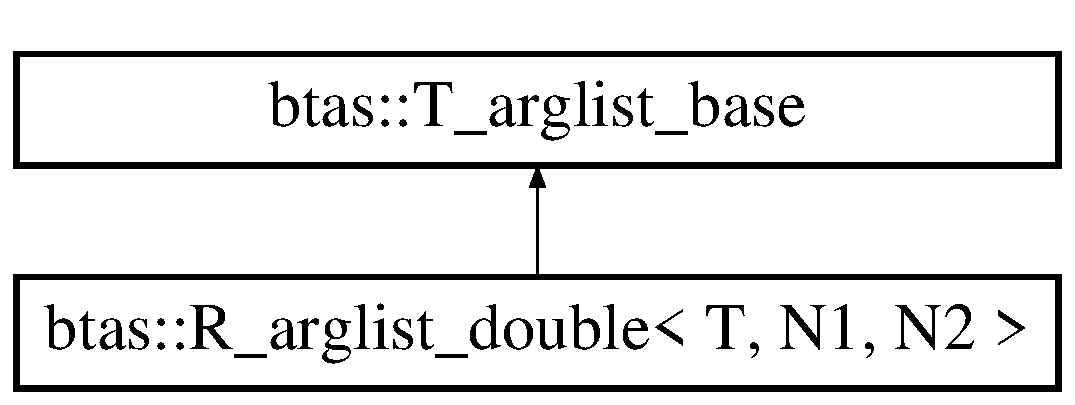
\includegraphics[height=2.000000cm]{d5/dcd/classbtas_1_1R__arglist__double}
\end{center}
\end{figure}
\subsection*{Public Member Functions}
\begin{DoxyCompactItemize}
\item 
{\bf R\-\_\-arglist\-\_\-double} ()
\begin{DoxyCompactList}\small\item\em Default constructor. \end{DoxyCompactList}\item 
virtual {\bf $\sim$\-R\-\_\-arglist\-\_\-double} ()
\begin{DoxyCompactList}\small\item\em Destructor. \end{DoxyCompactList}\item 
{\bf R\-\_\-arglist\-\_\-double} (const shared\-\_\-ptr$<$ {\bf T\-Array}$<$ T, N1 $>$$>$ \&arg1\-\_\-ptr, const shared\-\_\-ptr$<$ {\bf T\-Array}$<$ T, N2 $>$$>$ \&arg2\-\_\-ptr)
\begin{DoxyCompactList}\small\item\em Initializer. \end{DoxyCompactList}\item 
void {\bf reset} (const shared\-\_\-ptr$<$ {\bf T\-Array}$<$ T, N1 $>$$>$ \&arg1\-\_\-ptr, const shared\-\_\-ptr$<$ {\bf T\-Array}$<$ T, N2 $>$$>$ \&arg2\-\_\-ptr)
\begin{DoxyCompactList}\small\item\em Reset argment list. \end{DoxyCompactList}\end{DoxyCompactItemize}
\subsection*{Protected Member Functions}
\begin{DoxyCompactItemize}
\item 
virtual size\-\_\-t {\bf mf\-\_\-flops\-\_\-count} ()
\begin{DoxyCompactList}\small\item\em Function to compute F\-L\-O\-P\-S count. \end{DoxyCompactList}\end{DoxyCompactItemize}
\subsection*{Protected Attributes}
\begin{DoxyCompactItemize}
\item 
shared\-\_\-ptr$<$ {\bf T\-Array}$<$ T, N1 $>$ $>$ {\bf m\-\_\-argment\-\_\-1}
\item 
shared\-\_\-ptr$<$ {\bf T\-Array}$<$ T, N2 $>$ $>$ {\bf m\-\_\-argment\-\_\-2}
\end{DoxyCompactItemize}


\subsection{Detailed Description}
\subsubsection*{template$<$typename T, size\-\_\-t N1, size\-\_\-t N2$>$class btas\-::\-R\-\_\-arglist\-\_\-double$<$ T, N1, N2 $>$}

Replication argment list for double argments function. 

e.\-g. B\-L\-A\-S C\-O\-P\-Y, A\-X\-P\-Y 

Definition at line 81 of file Targlist.\-h.



\subsection{Constructor \& Destructor Documentation}
\index{btas\-::\-R\-\_\-arglist\-\_\-double@{btas\-::\-R\-\_\-arglist\-\_\-double}!R\-\_\-arglist\-\_\-double@{R\-\_\-arglist\-\_\-double}}
\index{R\-\_\-arglist\-\_\-double@{R\-\_\-arglist\-\_\-double}!btas::R_arglist_double@{btas\-::\-R\-\_\-arglist\-\_\-double}}
\subsubsection[{R\-\_\-arglist\-\_\-double}]{\setlength{\rightskip}{0pt plus 5cm}template$<$typename T, size\-\_\-t N1, size\-\_\-t N2$>$ {\bf btas\-::\-R\-\_\-arglist\-\_\-double}$<$ T, N1, N2 $>$\-::{\bf R\-\_\-arglist\-\_\-double} (
\begin{DoxyParamCaption}
{}
\end{DoxyParamCaption}
)\hspace{0.3cm}{\ttfamily [inline]}}\label{d5/dcd/classbtas_1_1R__arglist__double_a8d45c9abcf801a8c17c7443d8720f529}


Default constructor. 



Definition at line 89 of file Targlist.\-h.

\index{btas\-::\-R\-\_\-arglist\-\_\-double@{btas\-::\-R\-\_\-arglist\-\_\-double}!$\sim$\-R\-\_\-arglist\-\_\-double@{$\sim$\-R\-\_\-arglist\-\_\-double}}
\index{$\sim$\-R\-\_\-arglist\-\_\-double@{$\sim$\-R\-\_\-arglist\-\_\-double}!btas::R_arglist_double@{btas\-::\-R\-\_\-arglist\-\_\-double}}
\subsubsection[{$\sim$\-R\-\_\-arglist\-\_\-double}]{\setlength{\rightskip}{0pt plus 5cm}template$<$typename T, size\-\_\-t N1, size\-\_\-t N2$>$ virtual {\bf btas\-::\-R\-\_\-arglist\-\_\-double}$<$ T, N1, N2 $>$\-::$\sim${\bf R\-\_\-arglist\-\_\-double} (
\begin{DoxyParamCaption}
{}
\end{DoxyParamCaption}
)\hspace{0.3cm}{\ttfamily [inline]}, {\ttfamily [virtual]}}\label{d5/dcd/classbtas_1_1R__arglist__double_a7c08a3cbf1aeaaadb1b9f24823de3c59}


Destructor. 



Definition at line 91 of file Targlist.\-h.

\index{btas\-::\-R\-\_\-arglist\-\_\-double@{btas\-::\-R\-\_\-arglist\-\_\-double}!R\-\_\-arglist\-\_\-double@{R\-\_\-arglist\-\_\-double}}
\index{R\-\_\-arglist\-\_\-double@{R\-\_\-arglist\-\_\-double}!btas::R_arglist_double@{btas\-::\-R\-\_\-arglist\-\_\-double}}
\subsubsection[{R\-\_\-arglist\-\_\-double}]{\setlength{\rightskip}{0pt plus 5cm}template$<$typename T, size\-\_\-t N1, size\-\_\-t N2$>$ {\bf btas\-::\-R\-\_\-arglist\-\_\-double}$<$ T, N1, N2 $>$\-::{\bf R\-\_\-arglist\-\_\-double} (
\begin{DoxyParamCaption}
\item[{const shared\-\_\-ptr$<$ {\bf T\-Array}$<$ T, N1 $>$$>$ \&}]{arg1\-\_\-ptr, }
\item[{const shared\-\_\-ptr$<$ {\bf T\-Array}$<$ T, N2 $>$$>$ \&}]{arg2\-\_\-ptr}
\end{DoxyParamCaption}
)\hspace{0.3cm}{\ttfamily [inline]}}\label{d5/dcd/classbtas_1_1R__arglist__double_aa50ff2380ae55a6cec530bbf094274f8}


Initializer. 



Definition at line 94 of file Targlist.\-h.



\subsection{Member Function Documentation}
\index{btas\-::\-R\-\_\-arglist\-\_\-double@{btas\-::\-R\-\_\-arglist\-\_\-double}!mf\-\_\-flops\-\_\-count@{mf\-\_\-flops\-\_\-count}}
\index{mf\-\_\-flops\-\_\-count@{mf\-\_\-flops\-\_\-count}!btas::R_arglist_double@{btas\-::\-R\-\_\-arglist\-\_\-double}}
\subsubsection[{mf\-\_\-flops\-\_\-count}]{\setlength{\rightskip}{0pt plus 5cm}template$<$typename T, size\-\_\-t N1, size\-\_\-t N2$>$ virtual size\-\_\-t {\bf btas\-::\-R\-\_\-arglist\-\_\-double}$<$ T, N1, N2 $>$\-::mf\-\_\-flops\-\_\-count (
\begin{DoxyParamCaption}
{}
\end{DoxyParamCaption}
)\hspace{0.3cm}{\ttfamily [inline]}, {\ttfamily [protected]}, {\ttfamily [virtual]}}\label{d5/dcd/classbtas_1_1R__arglist__double_a84bad956959bf8d2c2b876c25bd06d2b}


Function to compute F\-L\-O\-P\-S count. 



Definition at line 86 of file Targlist.\-h.



Referenced by btas\-::\-R\-\_\-arglist\-\_\-double$<$ double, N, N $>$\-::\-R\-\_\-arglist\-\_\-double(), and btas\-::\-R\-\_\-arglist\-\_\-double$<$ double, N, N $>$\-::reset().

\index{btas\-::\-R\-\_\-arglist\-\_\-double@{btas\-::\-R\-\_\-arglist\-\_\-double}!reset@{reset}}
\index{reset@{reset}!btas::R_arglist_double@{btas\-::\-R\-\_\-arglist\-\_\-double}}
\subsubsection[{reset}]{\setlength{\rightskip}{0pt plus 5cm}template$<$typename T, size\-\_\-t N1, size\-\_\-t N2$>$ void {\bf btas\-::\-R\-\_\-arglist\-\_\-double}$<$ T, N1, N2 $>$\-::reset (
\begin{DoxyParamCaption}
\item[{const shared\-\_\-ptr$<$ {\bf T\-Array}$<$ T, N1 $>$$>$ \&}]{arg1\-\_\-ptr, }
\item[{const shared\-\_\-ptr$<$ {\bf T\-Array}$<$ T, N2 $>$$>$ \&}]{arg2\-\_\-ptr}
\end{DoxyParamCaption}
)\hspace{0.3cm}{\ttfamily [inline]}}\label{d5/dcd/classbtas_1_1R__arglist__double_a5bc9dc17df3a360c9bc2f9e6ecc52eae}


Reset argment list. 



Definition at line 102 of file Targlist.\-h.



Referenced by btas\-::\-Daxpy\-Arglist$<$ N $>$\-::reset(), and btas\-::\-Dpermute\-Arglist$<$ N $>$\-::reset().



\subsection{Field Documentation}
\index{btas\-::\-R\-\_\-arglist\-\_\-double@{btas\-::\-R\-\_\-arglist\-\_\-double}!m\-\_\-argment\-\_\-1@{m\-\_\-argment\-\_\-1}}
\index{m\-\_\-argment\-\_\-1@{m\-\_\-argment\-\_\-1}!btas::R_arglist_double@{btas\-::\-R\-\_\-arglist\-\_\-double}}
\subsubsection[{m\-\_\-argment\-\_\-1}]{\setlength{\rightskip}{0pt plus 5cm}template$<$typename T, size\-\_\-t N1, size\-\_\-t N2$>$ shared\-\_\-ptr$<${\bf T\-Array}$<$T, N1$>$ $>$ {\bf btas\-::\-R\-\_\-arglist\-\_\-double}$<$ T, N1, N2 $>$\-::m\-\_\-argment\-\_\-1\hspace{0.3cm}{\ttfamily [protected]}}\label{d5/dcd/classbtas_1_1R__arglist__double_aaa79f8a1486bbdd970a80758474532db}


Definition at line 83 of file Targlist.\-h.



Referenced by btas\-::\-R\-\_\-arglist\-\_\-double$<$ double, N, N $>$\-::mf\-\_\-flops\-\_\-count(), btas\-::\-R\-\_\-arglist\-\_\-double$<$ double, N, N $>$\-::\-R\-\_\-arglist\-\_\-double(), and btas\-::\-R\-\_\-arglist\-\_\-double$<$ double, N, N $>$\-::reset().

\index{btas\-::\-R\-\_\-arglist\-\_\-double@{btas\-::\-R\-\_\-arglist\-\_\-double}!m\-\_\-argment\-\_\-2@{m\-\_\-argment\-\_\-2}}
\index{m\-\_\-argment\-\_\-2@{m\-\_\-argment\-\_\-2}!btas::R_arglist_double@{btas\-::\-R\-\_\-arglist\-\_\-double}}
\subsubsection[{m\-\_\-argment\-\_\-2}]{\setlength{\rightskip}{0pt plus 5cm}template$<$typename T, size\-\_\-t N1, size\-\_\-t N2$>$ shared\-\_\-ptr$<${\bf T\-Array}$<$T, N2$>$ $>$ {\bf btas\-::\-R\-\_\-arglist\-\_\-double}$<$ T, N1, N2 $>$\-::m\-\_\-argment\-\_\-2\hspace{0.3cm}{\ttfamily [protected]}}\label{d5/dcd/classbtas_1_1R__arglist__double_ad6bf3381e21b264eacded62951903004}


Definition at line 84 of file Targlist.\-h.



Referenced by btas\-::\-R\-\_\-arglist\-\_\-double$<$ double, N, N $>$\-::\-R\-\_\-arglist\-\_\-double(), and btas\-::\-R\-\_\-arglist\-\_\-double$<$ double, N, N $>$\-::reset().



The documentation for this class was generated from the following file\-:\begin{DoxyCompactItemize}
\item 
include/btas/{\bf Targlist.\-h}\end{DoxyCompactItemize}

\section{btas\-:\-:R\-\_\-arglist\-\_\-quadra$<$ T, N1, N2, N3, N4 $>$ Class Template Reference}
\label{d4/dec/classbtas_1_1R__arglist__quadra}\index{btas\-::\-R\-\_\-arglist\-\_\-quadra$<$ T, N1, N2, N3, N4 $>$@{btas\-::\-R\-\_\-arglist\-\_\-quadra$<$ T, N1, N2, N3, N4 $>$}}


Replication argment list for quadruple argments function.  




{\ttfamily \#include $<$Targlist.\-h$>$}

Inheritance diagram for btas\-:\-:R\-\_\-arglist\-\_\-quadra$<$ T, N1, N2, N3, N4 $>$\-:\begin{figure}[H]
\begin{center}
\leavevmode
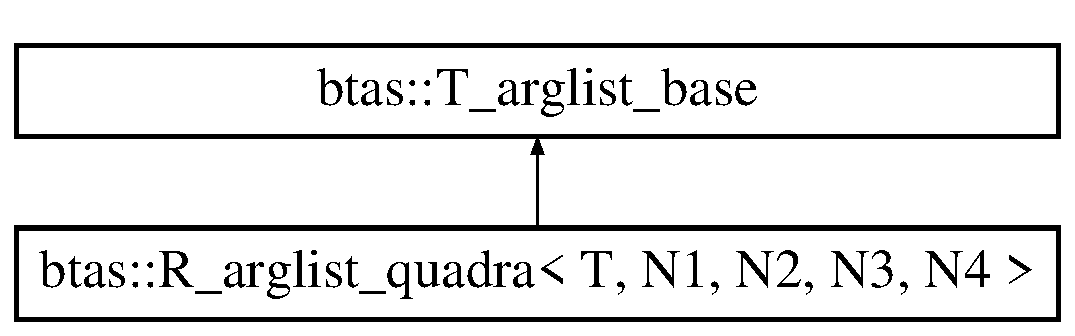
\includegraphics[height=2.000000cm]{d4/dec/classbtas_1_1R__arglist__quadra}
\end{center}
\end{figure}
\subsection*{Public Member Functions}
\begin{DoxyCompactItemize}
\item 
{\bf R\-\_\-arglist\-\_\-quadra} ()
\begin{DoxyCompactList}\small\item\em Default constructor. \end{DoxyCompactList}\item 
virtual {\bf $\sim$\-R\-\_\-arglist\-\_\-quadra} ()
\begin{DoxyCompactList}\small\item\em Destructor. \end{DoxyCompactList}\item 
{\bf R\-\_\-arglist\-\_\-quadra} (const shared\-\_\-ptr$<$ {\bf T\-Array}$<$ T, N1 $>$$>$ \&arg1\-\_\-ptr, const shared\-\_\-ptr$<$ {\bf T\-Array}$<$ T, N2 $>$$>$ \&arg2\-\_\-ptr, const shared\-\_\-ptr$<$ {\bf T\-Array}$<$ T, N3 $>$$>$ \&arg3\-\_\-ptr, const shared\-\_\-ptr$<$ {\bf T\-Array}$<$ T, N4 $>$$>$ \&arg4\-\_\-ptr)
\begin{DoxyCompactList}\small\item\em Initializer. \end{DoxyCompactList}\item 
void {\bf reset} (const shared\-\_\-ptr$<$ {\bf T\-Array}$<$ T, N1 $>$$>$ \&arg1\-\_\-ptr, const shared\-\_\-ptr$<$ {\bf T\-Array}$<$ T, N2 $>$$>$ \&arg2\-\_\-ptr, const shared\-\_\-ptr$<$ {\bf T\-Array}$<$ T, N3 $>$$>$ \&arg3\-\_\-ptr, const shared\-\_\-ptr$<$ {\bf T\-Array}$<$ T, N4 $>$$>$ \&arg4\-\_\-ptr)
\begin{DoxyCompactList}\small\item\em Reset argment list. \end{DoxyCompactList}\end{DoxyCompactItemize}
\subsection*{Protected Member Functions}
\begin{DoxyCompactItemize}
\item 
virtual size\-\_\-t {\bf mf\-\_\-flops\-\_\-count} ()
\begin{DoxyCompactList}\small\item\em Function to compute F\-L\-O\-P\-S count. \end{DoxyCompactList}\end{DoxyCompactItemize}
\subsection*{Protected Attributes}
\begin{DoxyCompactItemize}
\item 
shared\-\_\-ptr$<$ {\bf T\-Array}$<$ T, N1 $>$ $>$ {\bf m\-\_\-argment\-\_\-1}
\item 
shared\-\_\-ptr$<$ {\bf T\-Array}$<$ T, N2 $>$ $>$ {\bf m\-\_\-argment\-\_\-2}
\item 
shared\-\_\-ptr$<$ {\bf T\-Array}$<$ T, N3 $>$ $>$ {\bf m\-\_\-argment\-\_\-3}
\item 
shared\-\_\-ptr$<$ {\bf T\-Array}$<$ T, N4 $>$ $>$ {\bf m\-\_\-argment\-\_\-4}
\end{DoxyCompactItemize}


\subsection{Detailed Description}
\subsubsection*{template$<$typename T, size\-\_\-t N1, size\-\_\-t N2, size\-\_\-t N3, size\-\_\-t N4$>$class btas\-::\-R\-\_\-arglist\-\_\-quadra$<$ T, N1, N2, N3, N4 $>$}

Replication argment list for quadruple argments function. 

e.\-g. L\-A\-P\-A\-C\-K G\-E\-S\-V\-D etc. 

Definition at line 150 of file Targlist.\-h.



\subsection{Constructor \& Destructor Documentation}
\index{btas\-::\-R\-\_\-arglist\-\_\-quadra@{btas\-::\-R\-\_\-arglist\-\_\-quadra}!R\-\_\-arglist\-\_\-quadra@{R\-\_\-arglist\-\_\-quadra}}
\index{R\-\_\-arglist\-\_\-quadra@{R\-\_\-arglist\-\_\-quadra}!btas::R_arglist_quadra@{btas\-::\-R\-\_\-arglist\-\_\-quadra}}
\subsubsection[{R\-\_\-arglist\-\_\-quadra}]{\setlength{\rightskip}{0pt plus 5cm}template$<$typename T, size\-\_\-t N1, size\-\_\-t N2, size\-\_\-t N3, size\-\_\-t N4$>$ {\bf btas\-::\-R\-\_\-arglist\-\_\-quadra}$<$ T, N1, N2, N3, N4 $>$\-::{\bf R\-\_\-arglist\-\_\-quadra} (
\begin{DoxyParamCaption}
{}
\end{DoxyParamCaption}
)\hspace{0.3cm}{\ttfamily [inline]}}\label{d4/dec/classbtas_1_1R__arglist__quadra_af9bf5d91b814e53e0eaff902729ebe8c}


Default constructor. 



Definition at line 160 of file Targlist.\-h.

\index{btas\-::\-R\-\_\-arglist\-\_\-quadra@{btas\-::\-R\-\_\-arglist\-\_\-quadra}!$\sim$\-R\-\_\-arglist\-\_\-quadra@{$\sim$\-R\-\_\-arglist\-\_\-quadra}}
\index{$\sim$\-R\-\_\-arglist\-\_\-quadra@{$\sim$\-R\-\_\-arglist\-\_\-quadra}!btas::R_arglist_quadra@{btas\-::\-R\-\_\-arglist\-\_\-quadra}}
\subsubsection[{$\sim$\-R\-\_\-arglist\-\_\-quadra}]{\setlength{\rightskip}{0pt plus 5cm}template$<$typename T, size\-\_\-t N1, size\-\_\-t N2, size\-\_\-t N3, size\-\_\-t N4$>$ virtual {\bf btas\-::\-R\-\_\-arglist\-\_\-quadra}$<$ T, N1, N2, N3, N4 $>$\-::$\sim${\bf R\-\_\-arglist\-\_\-quadra} (
\begin{DoxyParamCaption}
{}
\end{DoxyParamCaption}
)\hspace{0.3cm}{\ttfamily [inline]}, {\ttfamily [virtual]}}\label{d4/dec/classbtas_1_1R__arglist__quadra_a588b5d2adfd24ae3fd9e2cf77e310de6}


Destructor. 



Definition at line 162 of file Targlist.\-h.

\index{btas\-::\-R\-\_\-arglist\-\_\-quadra@{btas\-::\-R\-\_\-arglist\-\_\-quadra}!R\-\_\-arglist\-\_\-quadra@{R\-\_\-arglist\-\_\-quadra}}
\index{R\-\_\-arglist\-\_\-quadra@{R\-\_\-arglist\-\_\-quadra}!btas::R_arglist_quadra@{btas\-::\-R\-\_\-arglist\-\_\-quadra}}
\subsubsection[{R\-\_\-arglist\-\_\-quadra}]{\setlength{\rightskip}{0pt plus 5cm}template$<$typename T, size\-\_\-t N1, size\-\_\-t N2, size\-\_\-t N3, size\-\_\-t N4$>$ {\bf btas\-::\-R\-\_\-arglist\-\_\-quadra}$<$ T, N1, N2, N3, N4 $>$\-::{\bf R\-\_\-arglist\-\_\-quadra} (
\begin{DoxyParamCaption}
\item[{const shared\-\_\-ptr$<$ {\bf T\-Array}$<$ T, N1 $>$$>$ \&}]{arg1\-\_\-ptr, }
\item[{const shared\-\_\-ptr$<$ {\bf T\-Array}$<$ T, N2 $>$$>$ \&}]{arg2\-\_\-ptr, }
\item[{const shared\-\_\-ptr$<$ {\bf T\-Array}$<$ T, N3 $>$$>$ \&}]{arg3\-\_\-ptr, }
\item[{const shared\-\_\-ptr$<$ {\bf T\-Array}$<$ T, N4 $>$$>$ \&}]{arg4\-\_\-ptr}
\end{DoxyParamCaption}
)\hspace{0.3cm}{\ttfamily [inline]}}\label{d4/dec/classbtas_1_1R__arglist__quadra_a8f886c6e81fa593c823bc794b3480f2a}


Initializer. 



Definition at line 165 of file Targlist.\-h.



\subsection{Member Function Documentation}
\index{btas\-::\-R\-\_\-arglist\-\_\-quadra@{btas\-::\-R\-\_\-arglist\-\_\-quadra}!mf\-\_\-flops\-\_\-count@{mf\-\_\-flops\-\_\-count}}
\index{mf\-\_\-flops\-\_\-count@{mf\-\_\-flops\-\_\-count}!btas::R_arglist_quadra@{btas\-::\-R\-\_\-arglist\-\_\-quadra}}
\subsubsection[{mf\-\_\-flops\-\_\-count}]{\setlength{\rightskip}{0pt plus 5cm}template$<$typename T, size\-\_\-t N1, size\-\_\-t N2, size\-\_\-t N3, size\-\_\-t N4$>$ virtual size\-\_\-t {\bf btas\-::\-R\-\_\-arglist\-\_\-quadra}$<$ T, N1, N2, N3, N4 $>$\-::mf\-\_\-flops\-\_\-count (
\begin{DoxyParamCaption}
{}
\end{DoxyParamCaption}
)\hspace{0.3cm}{\ttfamily [inline]}, {\ttfamily [protected]}, {\ttfamily [virtual]}}\label{d4/dec/classbtas_1_1R__arglist__quadra_a8b6264716aab613234a20d59b9a745ee}


Function to compute F\-L\-O\-P\-S count. 



Definition at line 157 of file Targlist.\-h.



Referenced by btas\-::\-R\-\_\-arglist\-\_\-quadra$<$ double, N\-A, 1, N\-U, N\-A-\/\-N\-U+2 $>$\-::\-R\-\_\-arglist\-\_\-quadra(), and btas\-::\-R\-\_\-arglist\-\_\-quadra$<$ double, N\-A, 1, N\-U, N\-A-\/\-N\-U+2 $>$\-::reset().

\index{btas\-::\-R\-\_\-arglist\-\_\-quadra@{btas\-::\-R\-\_\-arglist\-\_\-quadra}!reset@{reset}}
\index{reset@{reset}!btas::R_arglist_quadra@{btas\-::\-R\-\_\-arglist\-\_\-quadra}}
\subsubsection[{reset}]{\setlength{\rightskip}{0pt plus 5cm}template$<$typename T, size\-\_\-t N1, size\-\_\-t N2, size\-\_\-t N3, size\-\_\-t N4$>$ void {\bf btas\-::\-R\-\_\-arglist\-\_\-quadra}$<$ T, N1, N2, N3, N4 $>$\-::reset (
\begin{DoxyParamCaption}
\item[{const shared\-\_\-ptr$<$ {\bf T\-Array}$<$ T, N1 $>$$>$ \&}]{arg1\-\_\-ptr, }
\item[{const shared\-\_\-ptr$<$ {\bf T\-Array}$<$ T, N2 $>$$>$ \&}]{arg2\-\_\-ptr, }
\item[{const shared\-\_\-ptr$<$ {\bf T\-Array}$<$ T, N3 $>$$>$ \&}]{arg3\-\_\-ptr, }
\item[{const shared\-\_\-ptr$<$ {\bf T\-Array}$<$ T, N4 $>$$>$ \&}]{arg4\-\_\-ptr}
\end{DoxyParamCaption}
)\hspace{0.3cm}{\ttfamily [inline]}}\label{d4/dec/classbtas_1_1R__arglist__quadra_aa9330f4eb2de48d7e37a65dfb39fb11d}


Reset argment list. 



Definition at line 177 of file Targlist.\-h.



\subsection{Field Documentation}
\index{btas\-::\-R\-\_\-arglist\-\_\-quadra@{btas\-::\-R\-\_\-arglist\-\_\-quadra}!m\-\_\-argment\-\_\-1@{m\-\_\-argment\-\_\-1}}
\index{m\-\_\-argment\-\_\-1@{m\-\_\-argment\-\_\-1}!btas::R_arglist_quadra@{btas\-::\-R\-\_\-arglist\-\_\-quadra}}
\subsubsection[{m\-\_\-argment\-\_\-1}]{\setlength{\rightskip}{0pt plus 5cm}template$<$typename T, size\-\_\-t N1, size\-\_\-t N2, size\-\_\-t N3, size\-\_\-t N4$>$ shared\-\_\-ptr$<${\bf T\-Array}$<$T, N1$>$ $>$ {\bf btas\-::\-R\-\_\-arglist\-\_\-quadra}$<$ T, N1, N2, N3, N4 $>$\-::m\-\_\-argment\-\_\-1\hspace{0.3cm}{\ttfamily [protected]}}\label{d4/dec/classbtas_1_1R__arglist__quadra_a2f0401f3865812862ae057259a9c5a9c}


Definition at line 152 of file Targlist.\-h.



Referenced by btas\-::\-R\-\_\-arglist\-\_\-quadra$<$ double, N\-A, 1, N\-U, N\-A-\/\-N\-U+2 $>$\-::mf\-\_\-flops\-\_\-count(), btas\-::\-R\-\_\-arglist\-\_\-quadra$<$ double, N\-A, 1, N\-U, N\-A-\/\-N\-U+2 $>$\-::\-R\-\_\-arglist\-\_\-quadra(), and btas\-::\-R\-\_\-arglist\-\_\-quadra$<$ double, N\-A, 1, N\-U, N\-A-\/\-N\-U+2 $>$\-::reset().

\index{btas\-::\-R\-\_\-arglist\-\_\-quadra@{btas\-::\-R\-\_\-arglist\-\_\-quadra}!m\-\_\-argment\-\_\-2@{m\-\_\-argment\-\_\-2}}
\index{m\-\_\-argment\-\_\-2@{m\-\_\-argment\-\_\-2}!btas::R_arglist_quadra@{btas\-::\-R\-\_\-arglist\-\_\-quadra}}
\subsubsection[{m\-\_\-argment\-\_\-2}]{\setlength{\rightskip}{0pt plus 5cm}template$<$typename T, size\-\_\-t N1, size\-\_\-t N2, size\-\_\-t N3, size\-\_\-t N4$>$ shared\-\_\-ptr$<${\bf T\-Array}$<$T, N2$>$ $>$ {\bf btas\-::\-R\-\_\-arglist\-\_\-quadra}$<$ T, N1, N2, N3, N4 $>$\-::m\-\_\-argment\-\_\-2\hspace{0.3cm}{\ttfamily [protected]}}\label{d4/dec/classbtas_1_1R__arglist__quadra_aad9f4f0845bcf94d6d51da9dd50a3e0d}


Definition at line 153 of file Targlist.\-h.



Referenced by btas\-::\-R\-\_\-arglist\-\_\-quadra$<$ double, N\-A, 1, N\-U, N\-A-\/\-N\-U+2 $>$\-::\-R\-\_\-arglist\-\_\-quadra(), and btas\-::\-R\-\_\-arglist\-\_\-quadra$<$ double, N\-A, 1, N\-U, N\-A-\/\-N\-U+2 $>$\-::reset().

\index{btas\-::\-R\-\_\-arglist\-\_\-quadra@{btas\-::\-R\-\_\-arglist\-\_\-quadra}!m\-\_\-argment\-\_\-3@{m\-\_\-argment\-\_\-3}}
\index{m\-\_\-argment\-\_\-3@{m\-\_\-argment\-\_\-3}!btas::R_arglist_quadra@{btas\-::\-R\-\_\-arglist\-\_\-quadra}}
\subsubsection[{m\-\_\-argment\-\_\-3}]{\setlength{\rightskip}{0pt plus 5cm}template$<$typename T, size\-\_\-t N1, size\-\_\-t N2, size\-\_\-t N3, size\-\_\-t N4$>$ shared\-\_\-ptr$<${\bf T\-Array}$<$T, N3$>$ $>$ {\bf btas\-::\-R\-\_\-arglist\-\_\-quadra}$<$ T, N1, N2, N3, N4 $>$\-::m\-\_\-argment\-\_\-3\hspace{0.3cm}{\ttfamily [protected]}}\label{d4/dec/classbtas_1_1R__arglist__quadra_a63d0876f1f74b494690fd19d578bc95b}


Definition at line 154 of file Targlist.\-h.



Referenced by btas\-::\-R\-\_\-arglist\-\_\-quadra$<$ double, N\-A, 1, N\-U, N\-A-\/\-N\-U+2 $>$\-::\-R\-\_\-arglist\-\_\-quadra(), and btas\-::\-R\-\_\-arglist\-\_\-quadra$<$ double, N\-A, 1, N\-U, N\-A-\/\-N\-U+2 $>$\-::reset().

\index{btas\-::\-R\-\_\-arglist\-\_\-quadra@{btas\-::\-R\-\_\-arglist\-\_\-quadra}!m\-\_\-argment\-\_\-4@{m\-\_\-argment\-\_\-4}}
\index{m\-\_\-argment\-\_\-4@{m\-\_\-argment\-\_\-4}!btas::R_arglist_quadra@{btas\-::\-R\-\_\-arglist\-\_\-quadra}}
\subsubsection[{m\-\_\-argment\-\_\-4}]{\setlength{\rightskip}{0pt plus 5cm}template$<$typename T, size\-\_\-t N1, size\-\_\-t N2, size\-\_\-t N3, size\-\_\-t N4$>$ shared\-\_\-ptr$<${\bf T\-Array}$<$T, N4$>$ $>$ {\bf btas\-::\-R\-\_\-arglist\-\_\-quadra}$<$ T, N1, N2, N3, N4 $>$\-::m\-\_\-argment\-\_\-4\hspace{0.3cm}{\ttfamily [protected]}}\label{d4/dec/classbtas_1_1R__arglist__quadra_a933e9bb46c373bc1da02594338d5bf81}


Definition at line 155 of file Targlist.\-h.



Referenced by btas\-::\-R\-\_\-arglist\-\_\-quadra$<$ double, N\-A, 1, N\-U, N\-A-\/\-N\-U+2 $>$\-::\-R\-\_\-arglist\-\_\-quadra(), and btas\-::\-R\-\_\-arglist\-\_\-quadra$<$ double, N\-A, 1, N\-U, N\-A-\/\-N\-U+2 $>$\-::reset().



The documentation for this class was generated from the following file\-:\begin{DoxyCompactItemize}
\item 
include/btas/{\bf Targlist.\-h}\end{DoxyCompactItemize}

\section{btas\-:\-:R\-\_\-arglist\-\_\-single$<$ T, N1 $>$ Class Template Reference}
\label{d5/d3b/classbtas_1_1R__arglist__single}\index{btas\-::\-R\-\_\-arglist\-\_\-single$<$ T, N1 $>$@{btas\-::\-R\-\_\-arglist\-\_\-single$<$ T, N1 $>$}}


Replication argment list for single argment function.  




{\ttfamily \#include $<$Targlist.\-h$>$}

Inheritance diagram for btas\-:\-:R\-\_\-arglist\-\_\-single$<$ T, N1 $>$\-:\begin{figure}[H]
\begin{center}
\leavevmode
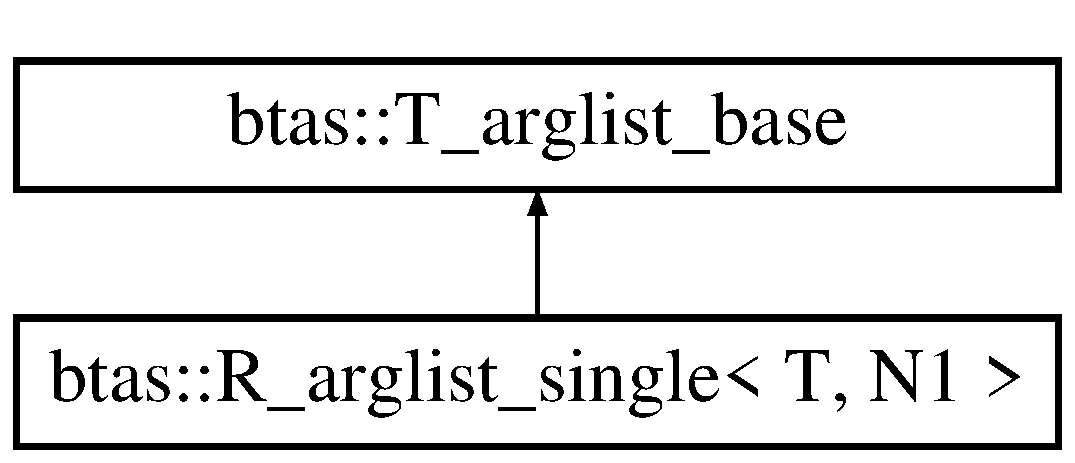
\includegraphics[height=2.000000cm]{d5/d3b/classbtas_1_1R__arglist__single}
\end{center}
\end{figure}
\subsection*{Public Member Functions}
\begin{DoxyCompactItemize}
\item 
{\bf R\-\_\-arglist\-\_\-single} ()
\begin{DoxyCompactList}\small\item\em Default constructor. \end{DoxyCompactList}\item 
virtual {\bf $\sim$\-R\-\_\-arglist\-\_\-single} ()
\begin{DoxyCompactList}\small\item\em Destructor. \end{DoxyCompactList}\item 
{\bf R\-\_\-arglist\-\_\-single} (const shared\-\_\-ptr$<$ {\bf T\-Array}$<$ T, N1 $>$$>$ \&arg1\-\_\-ptr)
\begin{DoxyCompactList}\small\item\em Initializer. \end{DoxyCompactList}\item 
void {\bf reset} (const shared\-\_\-ptr$<$ {\bf T\-Array}$<$ T, N1 $>$$>$ \&arg1\-\_\-ptr)
\begin{DoxyCompactList}\small\item\em Reset argment list. \end{DoxyCompactList}\end{DoxyCompactItemize}
\subsection*{Protected Member Functions}
\begin{DoxyCompactItemize}
\item 
virtual size\-\_\-t {\bf mf\-\_\-flops\-\_\-count} ()
\begin{DoxyCompactList}\small\item\em Function to compute F\-L\-O\-P\-S count. \end{DoxyCompactList}\end{DoxyCompactItemize}
\subsection*{Protected Attributes}
\begin{DoxyCompactItemize}
\item 
shared\-\_\-ptr$<$ {\bf T\-Array}$<$ T, N1 $>$ $>$ {\bf m\-\_\-argment\-\_\-1}
\end{DoxyCompactItemize}


\subsection{Detailed Description}
\subsubsection*{template$<$typename T, size\-\_\-t N1$>$class btas\-::\-R\-\_\-arglist\-\_\-single$<$ T, N1 $>$}

Replication argment list for single argment function. 

e.\-g. B\-L\-A\-S S\-C\-A\-L 

Definition at line 54 of file Targlist.\-h.



\subsection{Constructor \& Destructor Documentation}
\index{btas\-::\-R\-\_\-arglist\-\_\-single@{btas\-::\-R\-\_\-arglist\-\_\-single}!R\-\_\-arglist\-\_\-single@{R\-\_\-arglist\-\_\-single}}
\index{R\-\_\-arglist\-\_\-single@{R\-\_\-arglist\-\_\-single}!btas::R_arglist_single@{btas\-::\-R\-\_\-arglist\-\_\-single}}
\subsubsection[{R\-\_\-arglist\-\_\-single}]{\setlength{\rightskip}{0pt plus 5cm}template$<$typename T, size\-\_\-t N1$>$ {\bf btas\-::\-R\-\_\-arglist\-\_\-single}$<$ T, N1 $>$\-::{\bf R\-\_\-arglist\-\_\-single} (
\begin{DoxyParamCaption}
{}
\end{DoxyParamCaption}
)\hspace{0.3cm}{\ttfamily [inline]}}\label{d5/d3b/classbtas_1_1R__arglist__single_ada2f6f24721b5d2a056a81a107632dac}


Default constructor. 



Definition at line 61 of file Targlist.\-h.

\index{btas\-::\-R\-\_\-arglist\-\_\-single@{btas\-::\-R\-\_\-arglist\-\_\-single}!$\sim$\-R\-\_\-arglist\-\_\-single@{$\sim$\-R\-\_\-arglist\-\_\-single}}
\index{$\sim$\-R\-\_\-arglist\-\_\-single@{$\sim$\-R\-\_\-arglist\-\_\-single}!btas::R_arglist_single@{btas\-::\-R\-\_\-arglist\-\_\-single}}
\subsubsection[{$\sim$\-R\-\_\-arglist\-\_\-single}]{\setlength{\rightskip}{0pt plus 5cm}template$<$typename T, size\-\_\-t N1$>$ virtual {\bf btas\-::\-R\-\_\-arglist\-\_\-single}$<$ T, N1 $>$\-::$\sim${\bf R\-\_\-arglist\-\_\-single} (
\begin{DoxyParamCaption}
{}
\end{DoxyParamCaption}
)\hspace{0.3cm}{\ttfamily [inline]}, {\ttfamily [virtual]}}\label{d5/d3b/classbtas_1_1R__arglist__single_a1ea4cedc280d686b21fe330cce3f5c05}


Destructor. 



Definition at line 63 of file Targlist.\-h.

\index{btas\-::\-R\-\_\-arglist\-\_\-single@{btas\-::\-R\-\_\-arglist\-\_\-single}!R\-\_\-arglist\-\_\-single@{R\-\_\-arglist\-\_\-single}}
\index{R\-\_\-arglist\-\_\-single@{R\-\_\-arglist\-\_\-single}!btas::R_arglist_single@{btas\-::\-R\-\_\-arglist\-\_\-single}}
\subsubsection[{R\-\_\-arglist\-\_\-single}]{\setlength{\rightskip}{0pt plus 5cm}template$<$typename T, size\-\_\-t N1$>$ {\bf btas\-::\-R\-\_\-arglist\-\_\-single}$<$ T, N1 $>$\-::{\bf R\-\_\-arglist\-\_\-single} (
\begin{DoxyParamCaption}
\item[{const shared\-\_\-ptr$<$ {\bf T\-Array}$<$ T, N1 $>$$>$ \&}]{arg1\-\_\-ptr}
\end{DoxyParamCaption}
)\hspace{0.3cm}{\ttfamily [inline]}}\label{d5/d3b/classbtas_1_1R__arglist__single_a7bc77cbb0cdadb4865338c69394bea7d}


Initializer. 



Definition at line 66 of file Targlist.\-h.



\subsection{Member Function Documentation}
\index{btas\-::\-R\-\_\-arglist\-\_\-single@{btas\-::\-R\-\_\-arglist\-\_\-single}!mf\-\_\-flops\-\_\-count@{mf\-\_\-flops\-\_\-count}}
\index{mf\-\_\-flops\-\_\-count@{mf\-\_\-flops\-\_\-count}!btas::R_arglist_single@{btas\-::\-R\-\_\-arglist\-\_\-single}}
\subsubsection[{mf\-\_\-flops\-\_\-count}]{\setlength{\rightskip}{0pt plus 5cm}template$<$typename T, size\-\_\-t N1$>$ virtual size\-\_\-t {\bf btas\-::\-R\-\_\-arglist\-\_\-single}$<$ T, N1 $>$\-::mf\-\_\-flops\-\_\-count (
\begin{DoxyParamCaption}
{}
\end{DoxyParamCaption}
)\hspace{0.3cm}{\ttfamily [inline]}, {\ttfamily [protected]}, {\ttfamily [virtual]}}\label{d5/d3b/classbtas_1_1R__arglist__single_a1d580b7f24dbf1b8deabfb399d94ff75}


Function to compute F\-L\-O\-P\-S count. 



Definition at line 58 of file Targlist.\-h.



Referenced by btas\-::\-R\-\_\-arglist\-\_\-single$<$ double, N $>$\-::\-R\-\_\-arglist\-\_\-single(), and btas\-::\-R\-\_\-arglist\-\_\-single$<$ double, N $>$\-::reset().

\index{btas\-::\-R\-\_\-arglist\-\_\-single@{btas\-::\-R\-\_\-arglist\-\_\-single}!reset@{reset}}
\index{reset@{reset}!btas::R_arglist_single@{btas\-::\-R\-\_\-arglist\-\_\-single}}
\subsubsection[{reset}]{\setlength{\rightskip}{0pt plus 5cm}template$<$typename T, size\-\_\-t N1$>$ void {\bf btas\-::\-R\-\_\-arglist\-\_\-single}$<$ T, N1 $>$\-::reset (
\begin{DoxyParamCaption}
\item[{const shared\-\_\-ptr$<$ {\bf T\-Array}$<$ T, N1 $>$$>$ \&}]{arg1\-\_\-ptr}
\end{DoxyParamCaption}
)\hspace{0.3cm}{\ttfamily [inline]}}\label{d5/d3b/classbtas_1_1R__arglist__single_ac1f1c20c98434adb78200b5b66311dbb}


Reset argment list. 



Definition at line 72 of file Targlist.\-h.



Referenced by btas\-::\-Dscal\-Arglist$<$ N $>$\-::reset().



\subsection{Field Documentation}
\index{btas\-::\-R\-\_\-arglist\-\_\-single@{btas\-::\-R\-\_\-arglist\-\_\-single}!m\-\_\-argment\-\_\-1@{m\-\_\-argment\-\_\-1}}
\index{m\-\_\-argment\-\_\-1@{m\-\_\-argment\-\_\-1}!btas::R_arglist_single@{btas\-::\-R\-\_\-arglist\-\_\-single}}
\subsubsection[{m\-\_\-argment\-\_\-1}]{\setlength{\rightskip}{0pt plus 5cm}template$<$typename T, size\-\_\-t N1$>$ shared\-\_\-ptr$<${\bf T\-Array}$<$T, N1$>$ $>$ {\bf btas\-::\-R\-\_\-arglist\-\_\-single}$<$ T, N1 $>$\-::m\-\_\-argment\-\_\-1\hspace{0.3cm}{\ttfamily [protected]}}\label{d5/d3b/classbtas_1_1R__arglist__single_a494b1446b8550e2de5c2849aa5cf6cc5}


Definition at line 56 of file Targlist.\-h.



Referenced by btas\-::\-R\-\_\-arglist\-\_\-single$<$ double, N $>$\-::mf\-\_\-flops\-\_\-count(), btas\-::\-R\-\_\-arglist\-\_\-single$<$ double, N $>$\-::\-R\-\_\-arglist\-\_\-single(), and btas\-::\-R\-\_\-arglist\-\_\-single$<$ double, N $>$\-::reset().



The documentation for this class was generated from the following file\-:\begin{DoxyCompactItemize}
\item 
include/btas/{\bf Targlist.\-h}\end{DoxyCompactItemize}

\section{btas\-:\-:R\-\_\-arglist\-\_\-triple$<$ T, N1, N2, N3 $>$ Class Template Reference}
\label{dd/d0a/classbtas_1_1R__arglist__triple}\index{btas\-::\-R\-\_\-arglist\-\_\-triple$<$ T, N1, N2, N3 $>$@{btas\-::\-R\-\_\-arglist\-\_\-triple$<$ T, N1, N2, N3 $>$}}


Replication argment list for triple argments function.  




{\ttfamily \#include $<$Targlist.\-h$>$}

Inheritance diagram for btas\-:\-:R\-\_\-arglist\-\_\-triple$<$ T, N1, N2, N3 $>$\-:\begin{figure}[H]
\begin{center}
\leavevmode
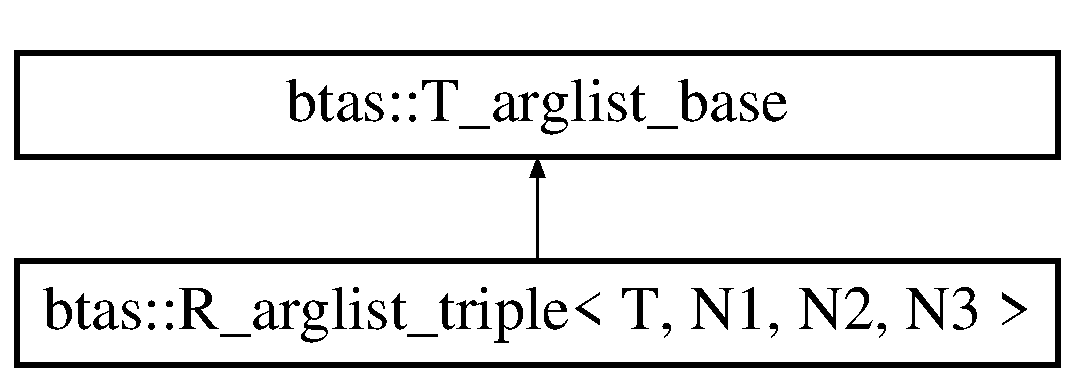
\includegraphics[height=2.000000cm]{dd/d0a/classbtas_1_1R__arglist__triple}
\end{center}
\end{figure}
\subsection*{Public Member Functions}
\begin{DoxyCompactItemize}
\item 
{\bf R\-\_\-arglist\-\_\-triple} ()
\begin{DoxyCompactList}\small\item\em Default constructor. \end{DoxyCompactList}\item 
virtual {\bf $\sim$\-R\-\_\-arglist\-\_\-triple} ()
\begin{DoxyCompactList}\small\item\em Destructor. \end{DoxyCompactList}\item 
{\bf R\-\_\-arglist\-\_\-triple} (const shared\-\_\-ptr$<$ {\bf T\-Array}$<$ T, N1 $>$$>$ \&arg1\-\_\-ptr, const shared\-\_\-ptr$<$ {\bf T\-Array}$<$ T, N2 $>$$>$ \&arg2\-\_\-ptr, const shared\-\_\-ptr$<$ {\bf T\-Array}$<$ T, N3 $>$$>$ \&arg3\-\_\-ptr)
\begin{DoxyCompactList}\small\item\em Initializer. \end{DoxyCompactList}\item 
void {\bf reset} (const shared\-\_\-ptr$<$ {\bf T\-Array}$<$ T, N1 $>$$>$ \&arg1\-\_\-ptr, const shared\-\_\-ptr$<$ {\bf T\-Array}$<$ T, N2 $>$$>$ \&arg2\-\_\-ptr, const shared\-\_\-ptr$<$ {\bf T\-Array}$<$ T, N3 $>$$>$ \&arg3\-\_\-ptr)
\begin{DoxyCompactList}\small\item\em Reset argment list. \end{DoxyCompactList}\end{DoxyCompactItemize}
\subsection*{Protected Member Functions}
\begin{DoxyCompactItemize}
\item 
virtual size\-\_\-t {\bf mf\-\_\-flops\-\_\-count} ()
\begin{DoxyCompactList}\small\item\em Function to compute F\-L\-O\-P\-S count. \end{DoxyCompactList}\end{DoxyCompactItemize}
\subsection*{Protected Attributes}
\begin{DoxyCompactItemize}
\item 
shared\-\_\-ptr$<$ {\bf T\-Array}$<$ T, N1 $>$ $>$ {\bf m\-\_\-argment\-\_\-1}
\item 
shared\-\_\-ptr$<$ {\bf T\-Array}$<$ T, N2 $>$ $>$ {\bf m\-\_\-argment\-\_\-2}
\item 
shared\-\_\-ptr$<$ {\bf T\-Array}$<$ T, N3 $>$ $>$ {\bf m\-\_\-argment\-\_\-3}
\end{DoxyCompactItemize}


\subsection{Detailed Description}
\subsubsection*{template$<$typename T, size\-\_\-t N1, size\-\_\-t N2, size\-\_\-t N3$>$class btas\-::\-R\-\_\-arglist\-\_\-triple$<$ T, N1, N2, N3 $>$}

Replication argment list for triple argments function. 

e.\-g. L\-A\-P\-A\-C\-K S\-Y\-E\-V, H\-E\-E\-V etc. 

Definition at line 113 of file Targlist.\-h.



\subsection{Constructor \& Destructor Documentation}
\index{btas\-::\-R\-\_\-arglist\-\_\-triple@{btas\-::\-R\-\_\-arglist\-\_\-triple}!R\-\_\-arglist\-\_\-triple@{R\-\_\-arglist\-\_\-triple}}
\index{R\-\_\-arglist\-\_\-triple@{R\-\_\-arglist\-\_\-triple}!btas::R_arglist_triple@{btas\-::\-R\-\_\-arglist\-\_\-triple}}
\subsubsection[{R\-\_\-arglist\-\_\-triple}]{\setlength{\rightskip}{0pt plus 5cm}template$<$typename T , size\-\_\-t N1, size\-\_\-t N2, size\-\_\-t N3$>$ {\bf btas\-::\-R\-\_\-arglist\-\_\-triple}$<$ T, N1, N2, N3 $>$\-::{\bf R\-\_\-arglist\-\_\-triple} (
\begin{DoxyParamCaption}
{}
\end{DoxyParamCaption}
)\hspace{0.3cm}{\ttfamily [inline]}}\label{dd/d0a/classbtas_1_1R__arglist__triple_a185cfe9ffb4ba4b89a847c8942a38c01}


Default constructor. 



Definition at line 122 of file Targlist.\-h.

\index{btas\-::\-R\-\_\-arglist\-\_\-triple@{btas\-::\-R\-\_\-arglist\-\_\-triple}!$\sim$\-R\-\_\-arglist\-\_\-triple@{$\sim$\-R\-\_\-arglist\-\_\-triple}}
\index{$\sim$\-R\-\_\-arglist\-\_\-triple@{$\sim$\-R\-\_\-arglist\-\_\-triple}!btas::R_arglist_triple@{btas\-::\-R\-\_\-arglist\-\_\-triple}}
\subsubsection[{$\sim$\-R\-\_\-arglist\-\_\-triple}]{\setlength{\rightskip}{0pt plus 5cm}template$<$typename T , size\-\_\-t N1, size\-\_\-t N2, size\-\_\-t N3$>$ virtual {\bf btas\-::\-R\-\_\-arglist\-\_\-triple}$<$ T, N1, N2, N3 $>$\-::$\sim${\bf R\-\_\-arglist\-\_\-triple} (
\begin{DoxyParamCaption}
{}
\end{DoxyParamCaption}
)\hspace{0.3cm}{\ttfamily [inline]}, {\ttfamily [virtual]}}\label{dd/d0a/classbtas_1_1R__arglist__triple_a867ba5bda97c042cccc131a77113957c}


Destructor. 



Definition at line 124 of file Targlist.\-h.

\index{btas\-::\-R\-\_\-arglist\-\_\-triple@{btas\-::\-R\-\_\-arglist\-\_\-triple}!R\-\_\-arglist\-\_\-triple@{R\-\_\-arglist\-\_\-triple}}
\index{R\-\_\-arglist\-\_\-triple@{R\-\_\-arglist\-\_\-triple}!btas::R_arglist_triple@{btas\-::\-R\-\_\-arglist\-\_\-triple}}
\subsubsection[{R\-\_\-arglist\-\_\-triple}]{\setlength{\rightskip}{0pt plus 5cm}template$<$typename T , size\-\_\-t N1, size\-\_\-t N2, size\-\_\-t N3$>$ {\bf btas\-::\-R\-\_\-arglist\-\_\-triple}$<$ T, N1, N2, N3 $>$\-::{\bf R\-\_\-arglist\-\_\-triple} (
\begin{DoxyParamCaption}
\item[{const shared\-\_\-ptr$<$ {\bf T\-Array}$<$ T, N1 $>$$>$ \&}]{arg1\-\_\-ptr, }
\item[{const shared\-\_\-ptr$<$ {\bf T\-Array}$<$ T, N2 $>$$>$ \&}]{arg2\-\_\-ptr, }
\item[{const shared\-\_\-ptr$<$ {\bf T\-Array}$<$ T, N3 $>$$>$ \&}]{arg3\-\_\-ptr}
\end{DoxyParamCaption}
)\hspace{0.3cm}{\ttfamily [inline]}}\label{dd/d0a/classbtas_1_1R__arglist__triple_a6f1f0cde83dca213dd132339cc9f7c2c}


Initializer. 



Definition at line 127 of file Targlist.\-h.



References btas\-::\-R\-\_\-arglist\-\_\-triple$<$ T, N1, N2, N3 $>$\-::m\-\_\-argment\-\_\-1, btas\-::\-R\-\_\-arglist\-\_\-triple$<$ T, N1, N2, N3 $>$\-::m\-\_\-argment\-\_\-2, btas\-::\-R\-\_\-arglist\-\_\-triple$<$ T, N1, N2, N3 $>$\-::m\-\_\-argment\-\_\-3, btas\-::\-T\-\_\-arglist\-\_\-base\-::m\-\_\-flops, and btas\-::\-R\-\_\-arglist\-\_\-triple$<$ T, N1, N2, N3 $>$\-::mf\-\_\-flops\-\_\-count().



\subsection{Member Function Documentation}
\index{btas\-::\-R\-\_\-arglist\-\_\-triple@{btas\-::\-R\-\_\-arglist\-\_\-triple}!mf\-\_\-flops\-\_\-count@{mf\-\_\-flops\-\_\-count}}
\index{mf\-\_\-flops\-\_\-count@{mf\-\_\-flops\-\_\-count}!btas::R_arglist_triple@{btas\-::\-R\-\_\-arglist\-\_\-triple}}
\subsubsection[{mf\-\_\-flops\-\_\-count}]{\setlength{\rightskip}{0pt plus 5cm}template$<$typename T , size\-\_\-t N1, size\-\_\-t N2, size\-\_\-t N3$>$ virtual size\-\_\-t {\bf btas\-::\-R\-\_\-arglist\-\_\-triple}$<$ T, N1, N2, N3 $>$\-::mf\-\_\-flops\-\_\-count (
\begin{DoxyParamCaption}
{}
\end{DoxyParamCaption}
)\hspace{0.3cm}{\ttfamily [inline]}, {\ttfamily [protected]}, {\ttfamily [virtual]}}\label{dd/d0a/classbtas_1_1R__arglist__triple_a36e357dfac4f735a46d883c21b5a7dc9}


Function to compute F\-L\-O\-P\-S count. 



Definition at line 119 of file Targlist.\-h.



References btas\-::\-R\-\_\-arglist\-\_\-triple$<$ T, N1, N2, N3 $>$\-::m\-\_\-argment\-\_\-1.



Referenced by btas\-::\-R\-\_\-arglist\-\_\-triple$<$ T, N1, N2, N3 $>$\-::\-R\-\_\-arglist\-\_\-triple(), and btas\-::\-R\-\_\-arglist\-\_\-triple$<$ T, N1, N2, N3 $>$\-::reset().

\index{btas\-::\-R\-\_\-arglist\-\_\-triple@{btas\-::\-R\-\_\-arglist\-\_\-triple}!reset@{reset}}
\index{reset@{reset}!btas::R_arglist_triple@{btas\-::\-R\-\_\-arglist\-\_\-triple}}
\subsubsection[{reset}]{\setlength{\rightskip}{0pt plus 5cm}template$<$typename T , size\-\_\-t N1, size\-\_\-t N2, size\-\_\-t N3$>$ void {\bf btas\-::\-R\-\_\-arglist\-\_\-triple}$<$ T, N1, N2, N3 $>$\-::reset (
\begin{DoxyParamCaption}
\item[{const shared\-\_\-ptr$<$ {\bf T\-Array}$<$ T, N1 $>$$>$ \&}]{arg1\-\_\-ptr, }
\item[{const shared\-\_\-ptr$<$ {\bf T\-Array}$<$ T, N2 $>$$>$ \&}]{arg2\-\_\-ptr, }
\item[{const shared\-\_\-ptr$<$ {\bf T\-Array}$<$ T, N3 $>$$>$ \&}]{arg3\-\_\-ptr}
\end{DoxyParamCaption}
)\hspace{0.3cm}{\ttfamily [inline]}}\label{dd/d0a/classbtas_1_1R__arglist__triple_ac026da34e1ab6e88a83c9d23be56bc53}


Reset argment list. 



Definition at line 137 of file Targlist.\-h.



References btas\-::\-R\-\_\-arglist\-\_\-triple$<$ T, N1, N2, N3 $>$\-::m\-\_\-argment\-\_\-1, btas\-::\-R\-\_\-arglist\-\_\-triple$<$ T, N1, N2, N3 $>$\-::m\-\_\-argment\-\_\-2, btas\-::\-R\-\_\-arglist\-\_\-triple$<$ T, N1, N2, N3 $>$\-::m\-\_\-argment\-\_\-3, btas\-::\-T\-\_\-arglist\-\_\-base\-::m\-\_\-flops, and btas\-::\-R\-\_\-arglist\-\_\-triple$<$ T, N1, N2, N3 $>$\-::mf\-\_\-flops\-\_\-count().



\subsection{Field Documentation}
\index{btas\-::\-R\-\_\-arglist\-\_\-triple@{btas\-::\-R\-\_\-arglist\-\_\-triple}!m\-\_\-argment\-\_\-1@{m\-\_\-argment\-\_\-1}}
\index{m\-\_\-argment\-\_\-1@{m\-\_\-argment\-\_\-1}!btas::R_arglist_triple@{btas\-::\-R\-\_\-arglist\-\_\-triple}}
\subsubsection[{m\-\_\-argment\-\_\-1}]{\setlength{\rightskip}{0pt plus 5cm}template$<$typename T , size\-\_\-t N1, size\-\_\-t N2, size\-\_\-t N3$>$ shared\-\_\-ptr$<${\bf T\-Array}$<$T, N1$>$ $>$ {\bf btas\-::\-R\-\_\-arglist\-\_\-triple}$<$ T, N1, N2, N3 $>$\-::m\-\_\-argment\-\_\-1\hspace{0.3cm}{\ttfamily [protected]}}\label{dd/d0a/classbtas_1_1R__arglist__triple_a0c1ef9115472c589a2f27bbc7a6976df}


Definition at line 115 of file Targlist.\-h.



Referenced by btas\-::\-R\-\_\-arglist\-\_\-triple$<$ T, N1, N2, N3 $>$\-::mf\-\_\-flops\-\_\-count(), btas\-::\-R\-\_\-arglist\-\_\-triple$<$ T, N1, N2, N3 $>$\-::\-R\-\_\-arglist\-\_\-triple(), and btas\-::\-R\-\_\-arglist\-\_\-triple$<$ T, N1, N2, N3 $>$\-::reset().

\index{btas\-::\-R\-\_\-arglist\-\_\-triple@{btas\-::\-R\-\_\-arglist\-\_\-triple}!m\-\_\-argment\-\_\-2@{m\-\_\-argment\-\_\-2}}
\index{m\-\_\-argment\-\_\-2@{m\-\_\-argment\-\_\-2}!btas::R_arglist_triple@{btas\-::\-R\-\_\-arglist\-\_\-triple}}
\subsubsection[{m\-\_\-argment\-\_\-2}]{\setlength{\rightskip}{0pt plus 5cm}template$<$typename T , size\-\_\-t N1, size\-\_\-t N2, size\-\_\-t N3$>$ shared\-\_\-ptr$<${\bf T\-Array}$<$T, N2$>$ $>$ {\bf btas\-::\-R\-\_\-arglist\-\_\-triple}$<$ T, N1, N2, N3 $>$\-::m\-\_\-argment\-\_\-2\hspace{0.3cm}{\ttfamily [protected]}}\label{dd/d0a/classbtas_1_1R__arglist__triple_a0dfde03a15e13f6f5c492389078a49d7}


Definition at line 116 of file Targlist.\-h.



Referenced by btas\-::\-R\-\_\-arglist\-\_\-triple$<$ T, N1, N2, N3 $>$\-::\-R\-\_\-arglist\-\_\-triple(), and btas\-::\-R\-\_\-arglist\-\_\-triple$<$ T, N1, N2, N3 $>$\-::reset().

\index{btas\-::\-R\-\_\-arglist\-\_\-triple@{btas\-::\-R\-\_\-arglist\-\_\-triple}!m\-\_\-argment\-\_\-3@{m\-\_\-argment\-\_\-3}}
\index{m\-\_\-argment\-\_\-3@{m\-\_\-argment\-\_\-3}!btas::R_arglist_triple@{btas\-::\-R\-\_\-arglist\-\_\-triple}}
\subsubsection[{m\-\_\-argment\-\_\-3}]{\setlength{\rightskip}{0pt plus 5cm}template$<$typename T , size\-\_\-t N1, size\-\_\-t N2, size\-\_\-t N3$>$ shared\-\_\-ptr$<${\bf T\-Array}$<$T, N3$>$ $>$ {\bf btas\-::\-R\-\_\-arglist\-\_\-triple}$<$ T, N1, N2, N3 $>$\-::m\-\_\-argment\-\_\-3\hspace{0.3cm}{\ttfamily [protected]}}\label{dd/d0a/classbtas_1_1R__arglist__triple_a547146621d7049e16fcd70133bd4267a}


Definition at line 117 of file Targlist.\-h.



Referenced by btas\-::\-R\-\_\-arglist\-\_\-triple$<$ T, N1, N2, N3 $>$\-::\-R\-\_\-arglist\-\_\-triple(), and btas\-::\-R\-\_\-arglist\-\_\-triple$<$ T, N1, N2, N3 $>$\-::reset().



The documentation for this class was generated from the following file\-:\begin{DoxyCompactItemize}
\item 
include/btas/{\bf Targlist.\-h}\end{DoxyCompactItemize}

\section{btas\-:\-:S\-T\-Array$<$ T, N $>$ Class Template Reference}
\label{d7/d05/classbtas_1_1STArray}\index{btas\-::\-S\-T\-Array$<$ T, N $>$@{btas\-::\-S\-T\-Array$<$ T, N $>$}}


Block-\/sparse array class.  




{\ttfamily \#include $<$S\-T\-Array.\-h$>$}

Inheritance diagram for btas\-:\-:S\-T\-Array$<$ T, N $>$\-:\begin{figure}[H]
\begin{center}
\leavevmode
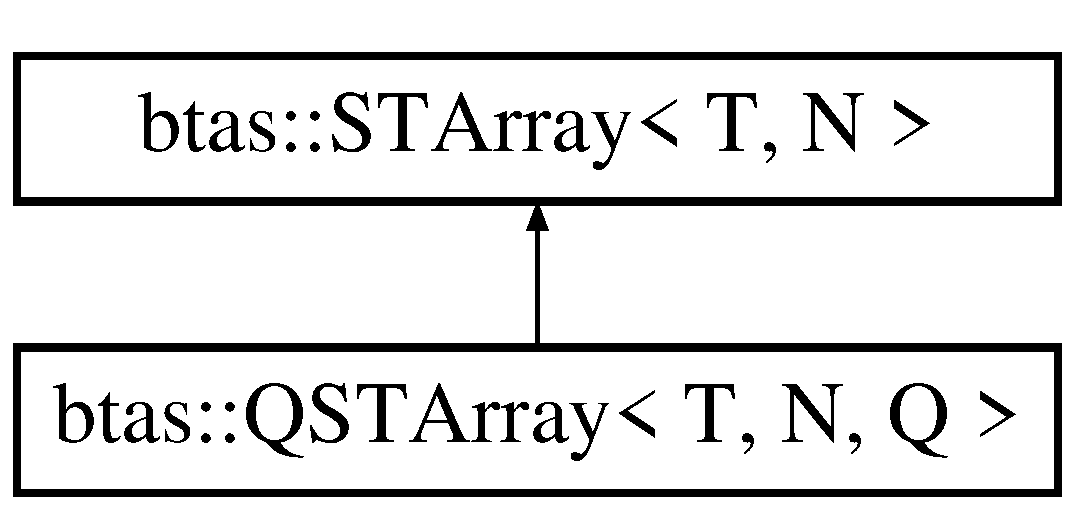
\includegraphics[height=2.000000cm]{d7/d05/classbtas_1_1STArray}
\end{center}
\end{figure}
\subsection*{Public Types}
\begin{DoxyCompactItemize}
\item 
typedef Data\-Type\-::const\-\_\-iterator {\bf const\-\_\-iterator}
\item 
typedef Data\-Type\-::iterator {\bf iterator}
\end{DoxyCompactItemize}
\subsection*{Public Member Functions}
\begin{DoxyCompactItemize}
\item 
{\bf S\-T\-Array} ()
\begin{DoxyCompactList}\small\item\em Default constructor. \end{DoxyCompactList}\item 
virtual {\bf $\sim$\-S\-T\-Array} ()
\begin{DoxyCompactList}\small\item\em Destructor. \end{DoxyCompactList}\item 
{\bf S\-T\-Array} (const {\bf I\-Vector}$<$ N $>$ \&\-\_\-shape)
\begin{DoxyCompactList}\small\item\em Construct by sparse-\/block shape. \end{DoxyCompactList}\item 
{\bf S\-T\-Array} (const {\bf T\-Vector}$<$ {\bf Dshapes}, N $>$ \&\-\_\-dn\-\_\-shape, bool \-\_\-allocate=true)
\begin{DoxyCompactList}\small\item\em Construct by dense-\/block shapes. \end{DoxyCompactList}\item 
{\bf S\-T\-Array} (const {\bf T\-Vector}$<$ {\bf Dshapes}, N $>$ \&\-\_\-dn\-\_\-shape, const T \&value)
\begin{DoxyCompactList}\small\item\em Construct by dense-\/block shapes and fill elements by value. \end{DoxyCompactList}\item 
{\footnotesize template$<$class Generator $>$ }\\{\bf S\-T\-Array} (const {\bf T\-Vector}$<$ {\bf Dshapes}, N $>$ \&\-\_\-dn\-\_\-shape, Generator gen)
\begin{DoxyCompactList}\small\item\em Construct by dense-\/block shapes and fill elements by gen() \end{DoxyCompactList}\item 
{\bf S\-T\-Array} (const {\bf S\-T\-Array} \&other)
\begin{DoxyCompactList}\small\item\em Copy constructor. \end{DoxyCompactList}\item 
{\bf S\-T\-Array} \& {\bf operator=} (const {\bf S\-T\-Array} \&other)
\begin{DoxyCompactList}\small\item\em Copy assignment operator. \end{DoxyCompactList}\item 
void {\bf copy} (const {\bf S\-T\-Array} \&other)
\begin{DoxyCompactList}\small\item\em Take deep copy of other. \end{DoxyCompactList}\item 
{\bf S\-T\-Array} ({\bf S\-T\-Array} \&\&other)
\begin{DoxyCompactList}\small\item\em Move constructor. \end{DoxyCompactList}\item 
{\bf S\-T\-Array} \& {\bf operator=} ({\bf S\-T\-Array} \&\&other)
\begin{DoxyCompactList}\small\item\em Move assignment operator. \end{DoxyCompactList}\item 
void {\bf reference} (const {\bf S\-T\-Array} \&other)
\begin{DoxyCompactList}\small\item\em make reference to other \end{DoxyCompactList}\item 
{\bf S\-T\-Array} {\bf subarray} (const {\bf T\-Vector}$<$ {\bf Dshapes}, N $>$ \&\-\_\-indxs) const 
\begin{DoxyCompactList}\small\item\em Make subarray reference. \end{DoxyCompactList}\item 
void {\bf resize} (const {\bf I\-Vector}$<$ N $>$ \&\-\_\-shape)
\begin{DoxyCompactList}\small\item\em Resize by sparse-\/block shape. \end{DoxyCompactList}\item 
void {\bf resize} (const {\bf T\-Vector}$<$ {\bf Dshapes}, N $>$ \&\-\_\-dn\-\_\-shape, bool \-\_\-allocate=true)
\begin{DoxyCompactList}\small\item\em Resize by dense-\/block shapes using this-\/$>$mf\-\_\-check\-\_\-allowed(index) \end{DoxyCompactList}\item 
void {\bf allocate} ()
\begin{DoxyCompactList}\small\item\em Allocate all allowed blocks (existed blocks are collapsed) \end{DoxyCompactList}\item 
void {\bf resize} (const {\bf T\-Vector}$<$ {\bf Dshapes}, N $>$ \&\-\_\-dn\-\_\-shape, const T \&value)
\begin{DoxyCompactList}\small\item\em Resize by dense-\/block shapes and fill all elements by value. \end{DoxyCompactList}\item 
{\footnotesize template$<$class Generator $>$ }\\void {\bf resize} (const {\bf T\-Vector}$<$ {\bf Dshapes}, N $>$ \&\-\_\-dn\-\_\-shape, Generator gen)
\begin{DoxyCompactList}\small\item\em Resize by dense-\/block shapes and fill all elements by gen() \end{DoxyCompactList}\item 
void {\bf fill} (const T \&value)
\begin{DoxyCompactList}\small\item\em fills all elements by value \end{DoxyCompactList}\item 
void {\bf operator=} (const T \&value)
\begin{DoxyCompactList}\small\item\em fills all elements by value \end{DoxyCompactList}\item 
{\footnotesize template$<$class Generator $>$ }\\void {\bf generate} (Generator gen)
\begin{DoxyCompactList}\small\item\em generates all elements by gen() \end{DoxyCompactList}\item 
{\bf iterator} {\bf erase} (const {\bf I\-Vector}$<$ N $>$ \&\-\_\-index)
\begin{DoxyCompactList}\small\item\em Erase certain block by index. \end{DoxyCompactList}\item 
{\bf iterator} {\bf erase} (const int \&\-\_\-tag)
\begin{DoxyCompactList}\small\item\em Erase certain block by tag. \end{DoxyCompactList}\item 
virtual void {\bf clear} ()
\begin{DoxyCompactList}\small\item\em Deallocation. \end{DoxyCompactList}\item 
virtual void {\bf erase} (int \-\_\-rank, int \-\_\-index\-\_\-erase)
\begin{DoxyCompactList}\small\item\em Erase blocks of which have certain index. \end{DoxyCompactList}\item 
{\bf I\-Vector}$<$ N $>$ {\bf index} (int \-\_\-tag) const 
\begin{DoxyCompactList}\small\item\em convert tag to index \end{DoxyCompactList}\item 
int {\bf tag} (const {\bf I\-Vector}$<$ N $>$ \&\-\_\-index) const 
\begin{DoxyCompactList}\small\item\em convert index to tag \end{DoxyCompactList}\item 
const {\bf I\-Vector}$<$ N $>$ \& {\bf shape} () const 
\begin{DoxyCompactList}\small\item\em Returns sparse-\/block shape. \end{DoxyCompactList}\item 
const int \& {\bf shape} (int i) const 
\begin{DoxyCompactList}\small\item\em Returns sparse-\/block shape for rank i. \end{DoxyCompactList}\item 
const {\bf I\-Vector}$<$ N $>$ \& {\bf stride} () const 
\begin{DoxyCompactList}\small\item\em Returns sparse-\/block stride. \end{DoxyCompactList}\item 
const int \& {\bf stride} (int i) const 
\begin{DoxyCompactList}\small\item\em Returns sparse-\/block stride for rank i. \end{DoxyCompactList}\item 
size\-\_\-t {\bf nnz} () const 
\begin{DoxyCompactList}\small\item\em Returns number of non-\/zero sparse-\/blocks. \end{DoxyCompactList}\item 
size\-\_\-t {\bf size} () const 
\begin{DoxyCompactList}\small\item\em Returns total number of sparse-\/blocks (includes zero blocks) \end{DoxyCompactList}\item 
const {\bf T\-Vector}$<$ {\bf Dshapes}, N $>$ \& {\bf dshape} () const 
\begin{DoxyCompactList}\small\item\em Returns dense-\/block shapes. \end{DoxyCompactList}\item 
const {\bf Dshapes} \& {\bf dshape} (int i) const 
\begin{DoxyCompactList}\small\item\em Returns dense-\/block shapes for rank i. \end{DoxyCompactList}\item 
const {\bf T\-Vector}$<$ {\bf Dshapes}, N $>$ \& {\bf check\-\_\-dshape} ()
\begin{DoxyCompactList}\small\item\em Check and update dense-\/block shapes. \end{DoxyCompactList}\item 
{\bf T\-Vector}$<$ {\bf Dshapes}, N $>$ {\bf check\-\_\-net\-\_\-dshape} () const 
\begin{DoxyCompactList}\small\item\em Calc. and return net dense-\/block shapes. \end{DoxyCompactList}\item 
{\bf const\-\_\-iterator} {\bf begin} () const 
\item 
{\bf iterator} {\bf begin} ()
\item 
{\bf const\-\_\-iterator} {\bf end} () const 
\item 
{\bf iterator} {\bf end} ()
\item 
{\bf const\-\_\-iterator} {\bf find} (const {\bf I\-Vector}$<$ N $>$ \&\-\_\-index) const 
\item 
{\bf iterator} {\bf find} (const {\bf I\-Vector}$<$ N $>$ \&\-\_\-index)
\item 
{\bf const\-\_\-iterator} {\bf lower\-\_\-bound} (const {\bf I\-Vector}$<$ N $>$ \&\-\_\-index) const 
\item 
{\bf iterator} {\bf lower\-\_\-bound} (const {\bf I\-Vector}$<$ N $>$ \&\-\_\-index)
\item 
{\bf const\-\_\-iterator} {\bf upper\-\_\-bound} (const {\bf I\-Vector}$<$ N $>$ \&\-\_\-index) const 
\item 
{\bf iterator} {\bf upper\-\_\-bound} (const {\bf I\-Vector}$<$ N $>$ \&\-\_\-index)
\item 
{\bf const\-\_\-iterator} {\bf find} (const int \&\-\_\-tag) const 
\item 
{\bf iterator} {\bf find} (const int \&\-\_\-tag)
\item 
{\bf const\-\_\-iterator} {\bf lower\-\_\-bound} (const int \&\-\_\-tag) const 
\item 
{\bf iterator} {\bf lower\-\_\-bound} (const int \&\-\_\-tag)
\item 
{\bf const\-\_\-iterator} {\bf upper\-\_\-bound} (const int \&\-\_\-tag) const 
\item 
{\bf iterator} {\bf upper\-\_\-bound} (const int \&\-\_\-tag)
\item 
bool {\bf allowed} (const int \&\-\_\-tag) const 
\begin{DoxyCompactList}\small\item\em return true if the requested block is non-\/zero, called by block tag \end{DoxyCompactList}\item 
bool {\bf allowed} (const {\bf I\-Vector}$<$ N $>$ \&\-\_\-index) const 
\begin{DoxyCompactList}\small\item\em return true if the requested block is non-\/zero, called by block index \end{DoxyCompactList}\item 
{\bf iterator} {\bf reserve} (const int \&\-\_\-tag)
\begin{DoxyCompactList}\small\item\em reserve non-\/zero block and return its iterator, by block tag \end{DoxyCompactList}\item 
{\bf iterator} {\bf reserve} (const {\bf I\-Vector}$<$ N $>$ \&\-\_\-index)
\begin{DoxyCompactList}\small\item\em reserve non-\/zero block and return its iterator, by block index \end{DoxyCompactList}\item 
{\bf iterator} {\bf insert} (const int \&\-\_\-tag, const {\bf T\-Array}$<$ T, N $>$ \&block)
\begin{DoxyCompactList}\small\item\em insert dense-\/array block and return its iterator, by block tag \end{DoxyCompactList}\item 
{\bf iterator} {\bf insert} (const {\bf I\-Vector}$<$ N $>$ \&\-\_\-index, const {\bf T\-Array}$<$ T, N $>$ \&block)
\begin{DoxyCompactList}\small\item\em insert dense-\/array block and return its iterator, by block index \end{DoxyCompactList}\item 
{\bf S\-T\-Array} {\bf transposed\-\_\-view} (int K) const 
\begin{DoxyCompactList}\small\item\em return reference in which the sparse-\/blocks are transposed \end{DoxyCompactList}\item 
{\bf S\-T\-Array} {\bf permuted\-\_\-view} (const {\bf I\-Vector}$<$ N $>$ \&pindex) const 
\begin{DoxyCompactList}\small\item\em return reference in which the sparse-\/blocks are permuted by pindex \end{DoxyCompactList}\end{DoxyCompactItemize}
\subsection*{Protected Member Functions}
\begin{DoxyCompactItemize}
\item 
virtual bool {\bf mf\-\_\-check\-\_\-allowed} (const {\bf I\-Vector}$<$ N $>$ \&\-\_\-index) const 
\begin{DoxyCompactList}\small\item\em Checking non-\/zero block. \end{DoxyCompactList}\item 
void {\bf mf\-\_\-check\-\_\-dshape} (const {\bf I\-Vector}$<$ N $>$ \&\-\_\-index, const {\bf I\-Vector}$<$ N $>$ \&\-\_\-shape)
\end{DoxyCompactItemize}
\subsection*{Protected Attributes}
\begin{DoxyCompactItemize}
\item 
{\bf I\-Vector}$<$ N $>$ {\bf m\-\_\-shape}
\begin{DoxyCompactList}\small\item\em sparse-\/block shape \end{DoxyCompactList}\item 
{\bf T\-Vector}$<$ {\bf Dshapes}, N $>$ {\bf m\-\_\-dn\-\_\-shape}
\begin{DoxyCompactList}\small\item\em dense-\/block shapes \end{DoxyCompactList}\item 
{\bf I\-Vector}$<$ N $>$ {\bf m\-\_\-stride}
\begin{DoxyCompactList}\small\item\em stride for sparse-\/block \end{DoxyCompactList}\item 
{\bf Data\-Type} {\bf m\-\_\-store}
\begin{DoxyCompactList}\small\item\em non-\/zero data array mapped by tag \end{DoxyCompactList}\end{DoxyCompactItemize}
\subsection*{Private Types}
\begin{DoxyCompactItemize}
\item 
typedef std\-::map$<$ int, \\*
shared\-\_\-ptr$<$ {\bf T\-Array}$<$ T, N $>$ $>$ $>$ {\bf Data\-Type}
\end{DoxyCompactItemize}
\subsection*{Private Member Functions}
\begin{DoxyCompactItemize}
\item 
{\footnotesize template$<$class Archive $>$ }\\void {\bf serialize} (Archive \&ar, const unsigned int version)
\end{DoxyCompactItemize}
\subsection*{Friends}
\begin{DoxyCompactItemize}
\item 
class {\bf boost\-::serialization\-::access}
\end{DoxyCompactItemize}


\subsection{Detailed Description}
\subsubsection*{template$<$typename T, size\-\_\-t N$>$class btas\-::\-S\-T\-Array$<$ T, N $>$}

Block-\/sparse array class. 

explain here for more detail 

Definition at line 26 of file S\-T\-Array.\-h.



\subsection{Member Typedef Documentation}
\index{btas\-::\-S\-T\-Array@{btas\-::\-S\-T\-Array}!const\-\_\-iterator@{const\-\_\-iterator}}
\index{const\-\_\-iterator@{const\-\_\-iterator}!btas::STArray@{btas\-::\-S\-T\-Array}}
\subsubsection[{const\-\_\-iterator}]{\setlength{\rightskip}{0pt plus 5cm}template$<$typename T, size\-\_\-t N$>$ typedef Data\-Type\-::const\-\_\-iterator {\bf btas\-::\-S\-T\-Array}$<$ T, N $>$\-::{\bf const\-\_\-iterator}}\label{d7/d05/classbtas_1_1STArray_aea95f4f4c94d262cbae35b66114e4a9d}


Definition at line 33 of file S\-T\-Array.\-h.

\index{btas\-::\-S\-T\-Array@{btas\-::\-S\-T\-Array}!Data\-Type@{Data\-Type}}
\index{Data\-Type@{Data\-Type}!btas::STArray@{btas\-::\-S\-T\-Array}}
\subsubsection[{Data\-Type}]{\setlength{\rightskip}{0pt plus 5cm}template$<$typename T, size\-\_\-t N$>$ typedef std\-::map$<$int, shared\-\_\-ptr$<${\bf T\-Array}$<$T, N$>$ $>$ $>$ {\bf btas\-::\-S\-T\-Array}$<$ T, N $>$\-::{\bf Data\-Type}\hspace{0.3cm}{\ttfamily [private]}}\label{d7/d05/classbtas_1_1STArray_afae35b5f4e73e901f012e3f7d7dc3619}


Definition at line 29 of file S\-T\-Array.\-h.

\index{btas\-::\-S\-T\-Array@{btas\-::\-S\-T\-Array}!iterator@{iterator}}
\index{iterator@{iterator}!btas::STArray@{btas\-::\-S\-T\-Array}}
\subsubsection[{iterator}]{\setlength{\rightskip}{0pt plus 5cm}template$<$typename T, size\-\_\-t N$>$ typedef Data\-Type\-::iterator {\bf btas\-::\-S\-T\-Array}$<$ T, N $>$\-::{\bf iterator}}\label{d7/d05/classbtas_1_1STArray_a6243d24cd9aafe2fafba48c105094930}


Definition at line 34 of file S\-T\-Array.\-h.



\subsection{Constructor \& Destructor Documentation}
\index{btas\-::\-S\-T\-Array@{btas\-::\-S\-T\-Array}!S\-T\-Array@{S\-T\-Array}}
\index{S\-T\-Array@{S\-T\-Array}!btas::STArray@{btas\-::\-S\-T\-Array}}
\subsubsection[{S\-T\-Array}]{\setlength{\rightskip}{0pt plus 5cm}template$<$typename T, size\-\_\-t N$>$ {\bf btas\-::\-S\-T\-Array}$<$ T, N $>$\-::{\bf S\-T\-Array} (
\begin{DoxyParamCaption}
{}
\end{DoxyParamCaption}
)\hspace{0.3cm}{\ttfamily [inline]}}\label{d7/d05/classbtas_1_1STArray_a1b0b03835a5deac0d94b35e89979ea9e}


Default constructor. 



Definition at line 65 of file S\-T\-Array.\-h.



References btas\-::\-S\-T\-Array$<$ T, N $>$\-::m\-\_\-shape, and btas\-::\-S\-T\-Array$<$ T, N $>$\-::m\-\_\-stride.

\index{btas\-::\-S\-T\-Array@{btas\-::\-S\-T\-Array}!$\sim$\-S\-T\-Array@{$\sim$\-S\-T\-Array}}
\index{$\sim$\-S\-T\-Array@{$\sim$\-S\-T\-Array}!btas::STArray@{btas\-::\-S\-T\-Array}}
\subsubsection[{$\sim$\-S\-T\-Array}]{\setlength{\rightskip}{0pt plus 5cm}template$<$typename T, size\-\_\-t N$>$ virtual {\bf btas\-::\-S\-T\-Array}$<$ T, N $>$\-::$\sim${\bf S\-T\-Array} (
\begin{DoxyParamCaption}
{}
\end{DoxyParamCaption}
)\hspace{0.3cm}{\ttfamily [inline]}, {\ttfamily [virtual]}}\label{d7/d05/classbtas_1_1STArray_ad8b5b6bdc0d2ff2c3ccd8c708f9cedec}


Destructor. 



Definition at line 68 of file S\-T\-Array.\-h.

\index{btas\-::\-S\-T\-Array@{btas\-::\-S\-T\-Array}!S\-T\-Array@{S\-T\-Array}}
\index{S\-T\-Array@{S\-T\-Array}!btas::STArray@{btas\-::\-S\-T\-Array}}
\subsubsection[{S\-T\-Array}]{\setlength{\rightskip}{0pt plus 5cm}template$<$typename T, size\-\_\-t N$>$ {\bf btas\-::\-S\-T\-Array}$<$ T, N $>$\-::{\bf S\-T\-Array} (
\begin{DoxyParamCaption}
\item[{const {\bf I\-Vector}$<$ N $>$ \&}]{\-\_\-shape}
\end{DoxyParamCaption}
)\hspace{0.3cm}{\ttfamily [inline]}}\label{d7/d05/classbtas_1_1STArray_a1f681672cdb7a6f530db156851a9f393}


Construct by sparse-\/block shape. 



Definition at line 71 of file S\-T\-Array.\-h.



References btas\-::\-S\-T\-Array$<$ T, N $>$\-::resize().

\index{btas\-::\-S\-T\-Array@{btas\-::\-S\-T\-Array}!S\-T\-Array@{S\-T\-Array}}
\index{S\-T\-Array@{S\-T\-Array}!btas::STArray@{btas\-::\-S\-T\-Array}}
\subsubsection[{S\-T\-Array}]{\setlength{\rightskip}{0pt plus 5cm}template$<$typename T, size\-\_\-t N$>$ {\bf btas\-::\-S\-T\-Array}$<$ T, N $>$\-::{\bf S\-T\-Array} (
\begin{DoxyParamCaption}
\item[{const {\bf T\-Vector}$<$ {\bf Dshapes}, N $>$ \&}]{\-\_\-dn\-\_\-shape, }
\item[{bool}]{\-\_\-allocate = {\ttfamily true}}
\end{DoxyParamCaption}
)\hspace{0.3cm}{\ttfamily [inline]}}\label{d7/d05/classbtas_1_1STArray_a5829c8c74f93adab54630f8143c452fd}


Construct by dense-\/block shapes. 



Definition at line 74 of file S\-T\-Array.\-h.



References btas\-::\-S\-T\-Array$<$ T, N $>$\-::resize().

\index{btas\-::\-S\-T\-Array@{btas\-::\-S\-T\-Array}!S\-T\-Array@{S\-T\-Array}}
\index{S\-T\-Array@{S\-T\-Array}!btas::STArray@{btas\-::\-S\-T\-Array}}
\subsubsection[{S\-T\-Array}]{\setlength{\rightskip}{0pt plus 5cm}template$<$typename T, size\-\_\-t N$>$ {\bf btas\-::\-S\-T\-Array}$<$ T, N $>$\-::{\bf S\-T\-Array} (
\begin{DoxyParamCaption}
\item[{const {\bf T\-Vector}$<$ {\bf Dshapes}, N $>$ \&}]{\-\_\-dn\-\_\-shape, }
\item[{const T \&}]{value}
\end{DoxyParamCaption}
)\hspace{0.3cm}{\ttfamily [inline]}}\label{d7/d05/classbtas_1_1STArray_ae666e88320366e056a5d7bfdd639f34c}


Construct by dense-\/block shapes and fill elements by value. 



Definition at line 77 of file S\-T\-Array.\-h.



References btas\-::\-S\-T\-Array$<$ T, N $>$\-::resize().

\index{btas\-::\-S\-T\-Array@{btas\-::\-S\-T\-Array}!S\-T\-Array@{S\-T\-Array}}
\index{S\-T\-Array@{S\-T\-Array}!btas::STArray@{btas\-::\-S\-T\-Array}}
\subsubsection[{S\-T\-Array}]{\setlength{\rightskip}{0pt plus 5cm}template$<$typename T, size\-\_\-t N$>$ template$<$class Generator $>$ {\bf btas\-::\-S\-T\-Array}$<$ T, N $>$\-::{\bf S\-T\-Array} (
\begin{DoxyParamCaption}
\item[{const {\bf T\-Vector}$<$ {\bf Dshapes}, N $>$ \&}]{\-\_\-dn\-\_\-shape, }
\item[{Generator}]{gen}
\end{DoxyParamCaption}
)\hspace{0.3cm}{\ttfamily [inline]}}\label{d7/d05/classbtas_1_1STArray_aa52e7e65b382e281208c47ac9357c8c6}


Construct by dense-\/block shapes and fill elements by gen() 



Definition at line 81 of file S\-T\-Array.\-h.



References btas\-::\-S\-T\-Array$<$ T, N $>$\-::resize().

\index{btas\-::\-S\-T\-Array@{btas\-::\-S\-T\-Array}!S\-T\-Array@{S\-T\-Array}}
\index{S\-T\-Array@{S\-T\-Array}!btas::STArray@{btas\-::\-S\-T\-Array}}
\subsubsection[{S\-T\-Array}]{\setlength{\rightskip}{0pt plus 5cm}template$<$typename T, size\-\_\-t N$>$ {\bf btas\-::\-S\-T\-Array}$<$ T, N $>$\-::{\bf S\-T\-Array} (
\begin{DoxyParamCaption}
\item[{const {\bf S\-T\-Array}$<$ T, N $>$ \&}]{other}
\end{DoxyParamCaption}
)\hspace{0.3cm}{\ttfamily [inline]}}\label{d7/d05/classbtas_1_1STArray_a2560b9c2b357f30010c03fc5a68d3262}


Copy constructor. 



Definition at line 88 of file S\-T\-Array.\-h.



References btas\-::\-S\-T\-Array$<$ T, N $>$\-::copy().

\index{btas\-::\-S\-T\-Array@{btas\-::\-S\-T\-Array}!S\-T\-Array@{S\-T\-Array}}
\index{S\-T\-Array@{S\-T\-Array}!btas::STArray@{btas\-::\-S\-T\-Array}}
\subsubsection[{S\-T\-Array}]{\setlength{\rightskip}{0pt plus 5cm}template$<$typename T, size\-\_\-t N$>$ {\bf btas\-::\-S\-T\-Array}$<$ T, N $>$\-::{\bf S\-T\-Array} (
\begin{DoxyParamCaption}
\item[{{\bf S\-T\-Array}$<$ T, N $>$ \&\&}]{other}
\end{DoxyParamCaption}
)\hspace{0.3cm}{\ttfamily [inline]}}\label{d7/d05/classbtas_1_1STArray_a581ff9c609c855a01a8e8e79f5d8780a}


Move constructor. 



Definition at line 111 of file S\-T\-Array.\-h.



References btas\-::\-S\-T\-Array$<$ T, N $>$\-::m\-\_\-dn\-\_\-shape, btas\-::\-S\-T\-Array$<$ T, N $>$\-::m\-\_\-shape, btas\-::\-S\-T\-Array$<$ T, N $>$\-::m\-\_\-store, and btas\-::\-S\-T\-Array$<$ T, N $>$\-::m\-\_\-stride.



\subsection{Member Function Documentation}
\index{btas\-::\-S\-T\-Array@{btas\-::\-S\-T\-Array}!allocate@{allocate}}
\index{allocate@{allocate}!btas::STArray@{btas\-::\-S\-T\-Array}}
\subsubsection[{allocate}]{\setlength{\rightskip}{0pt plus 5cm}template$<$typename T, size\-\_\-t N$>$ void {\bf btas\-::\-S\-T\-Array}$<$ T, N $>$\-::allocate (
\begin{DoxyParamCaption}
{}
\end{DoxyParamCaption}
)\hspace{0.3cm}{\ttfamily [inline]}}\label{d7/d05/classbtas_1_1STArray_a9c8c97258a84ddbfa4daf1cd1f41cc28}


Allocate all allowed blocks (existed blocks are collapsed) 



Definition at line 214 of file S\-T\-Array.\-h.



References btas\-::\-S\-T\-Array$<$ T, N $>$\-::m\-\_\-dn\-\_\-shape, btas\-::\-S\-T\-Array$<$ T, N $>$\-::m\-\_\-shape, btas\-::\-S\-T\-Array$<$ T, N $>$\-::m\-\_\-store, btas\-::\-S\-T\-Array$<$ T, N $>$\-::mf\-\_\-check\-\_\-allowed(), and btas\-::\-S\-T\-Array$<$ T, N $>$\-::size().



Referenced by btas\-::\-S\-T\-Array$<$ T, N $>$\-::resize().

\index{btas\-::\-S\-T\-Array@{btas\-::\-S\-T\-Array}!allowed@{allowed}}
\index{allowed@{allowed}!btas::STArray@{btas\-::\-S\-T\-Array}}
\subsubsection[{allowed}]{\setlength{\rightskip}{0pt plus 5cm}template$<$typename T, size\-\_\-t N$>$ bool {\bf btas\-::\-S\-T\-Array}$<$ T, N $>$\-::allowed (
\begin{DoxyParamCaption}
\item[{const int \&}]{\-\_\-tag}
\end{DoxyParamCaption}
) const\hspace{0.3cm}{\ttfamily [inline]}}\label{d7/d05/classbtas_1_1STArray_a9d41dfdb0103fe7469f1f944562b8929}


return true if the requested block is non-\/zero, called by block tag 



Definition at line 432 of file S\-T\-Array.\-h.



References btas\-::\-S\-T\-Array$<$ T, N $>$\-::index(), and btas\-::\-S\-T\-Array$<$ T, N $>$\-::mf\-\_\-check\-\_\-allowed().



Referenced by btas\-::\-Q\-S\-Tmerge(), btas\-::thread\-\_\-\-S\-Dgemm(), btas\-::thread\-\_\-\-S\-Dgemv(), and btas\-::thread\-\_\-\-S\-Dger().

\index{btas\-::\-S\-T\-Array@{btas\-::\-S\-T\-Array}!allowed@{allowed}}
\index{allowed@{allowed}!btas::STArray@{btas\-::\-S\-T\-Array}}
\subsubsection[{allowed}]{\setlength{\rightskip}{0pt plus 5cm}template$<$typename T, size\-\_\-t N$>$ bool {\bf btas\-::\-S\-T\-Array}$<$ T, N $>$\-::allowed (
\begin{DoxyParamCaption}
\item[{const {\bf I\-Vector}$<$ N $>$ \&}]{\-\_\-index}
\end{DoxyParamCaption}
) const\hspace{0.3cm}{\ttfamily [inline]}}\label{d7/d05/classbtas_1_1STArray_a357b76a1233a735e4590eb209f7a8743}


return true if the requested block is non-\/zero, called by block index 



Definition at line 434 of file S\-T\-Array.\-h.



References btas\-::\-S\-T\-Array$<$ T, N $>$\-::mf\-\_\-check\-\_\-allowed().

\index{btas\-::\-S\-T\-Array@{btas\-::\-S\-T\-Array}!begin@{begin}}
\index{begin@{begin}!btas::STArray@{btas\-::\-S\-T\-Array}}
\subsubsection[{begin}]{\setlength{\rightskip}{0pt plus 5cm}template$<$typename T, size\-\_\-t N$>$ {\bf const\-\_\-iterator} {\bf btas\-::\-S\-T\-Array}$<$ T, N $>$\-::begin (
\begin{DoxyParamCaption}
{}
\end{DoxyParamCaption}
) const\hspace{0.3cm}{\ttfamily [inline]}}\label{d7/d05/classbtas_1_1STArray_a95a5abb1d8532b3544cb2750e0cba94c}


Definition at line 403 of file S\-T\-Array.\-h.



References btas\-::\-S\-T\-Array$<$ T, N $>$\-::m\-\_\-store.



Referenced by mps\-::dot(), btas\-::\-Q\-S\-T\-Array$<$ T, N, Q $>$\-::erase(), mps\-::inprod(), btas\-::\-Q\-S\-T\-Array$<$ T, N, Q $>$\-::parity(), btas\-::\-Q\-S\-Dgesvd(), btas\-::\-Q\-S\-Texpand(), btas\-::\-S\-Ddiagonal(), btas\-::\-S\-Ddidm(), btas\-::\-S\-Ddimd(), btas\-::serial\-\_\-\-S\-Daxpy(), btas\-::serial\-\_\-\-S\-Dcopy(), btas\-::serial\-\_\-\-S\-Ddot(), btas\-::serial\-\_\-\-S\-Dpermute(), btas\-::serial\-\_\-\-S\-Dscal(), btas\-::\-S\-Tdsum(), btas\-::thread\-\_\-\-Q\-S\-Dgesvd(), btas\-::thread\-\_\-\-S\-Daxpy(), btas\-::thread\-\_\-\-S\-Dcopy(), btas\-::thread\-\_\-\-S\-Dger(), btas\-::thread\-\_\-\-S\-Dpermute(), and btas\-::thread\-\_\-\-S\-Dscal().

\index{btas\-::\-S\-T\-Array@{btas\-::\-S\-T\-Array}!begin@{begin}}
\index{begin@{begin}!btas::STArray@{btas\-::\-S\-T\-Array}}
\subsubsection[{begin}]{\setlength{\rightskip}{0pt plus 5cm}template$<$typename T, size\-\_\-t N$>$ {\bf iterator} {\bf btas\-::\-S\-T\-Array}$<$ T, N $>$\-::begin (
\begin{DoxyParamCaption}
{}
\end{DoxyParamCaption}
)\hspace{0.3cm}{\ttfamily [inline]}}\label{d7/d05/classbtas_1_1STArray_aab14034e1bf08d5a8ff7fedd6ced5a3a}


Definition at line 404 of file S\-T\-Array.\-h.



References btas\-::\-S\-T\-Array$<$ T, N $>$\-::m\-\_\-store.

\index{btas\-::\-S\-T\-Array@{btas\-::\-S\-T\-Array}!check\-\_\-dshape@{check\-\_\-dshape}}
\index{check\-\_\-dshape@{check\-\_\-dshape}!btas::STArray@{btas\-::\-S\-T\-Array}}
\subsubsection[{check\-\_\-dshape}]{\setlength{\rightskip}{0pt plus 5cm}template$<$typename T, size\-\_\-t N$>$ const {\bf T\-Vector}$<${\bf Dshapes}, N$>$\& {\bf btas\-::\-S\-T\-Array}$<$ T, N $>$\-::check\-\_\-dshape (
\begin{DoxyParamCaption}
{}
\end{DoxyParamCaption}
)\hspace{0.3cm}{\ttfamily [inline]}}\label{d7/d05/classbtas_1_1STArray_a3cdec7beeb57b2c266ed7aa8a511a1b4}


Check and update dense-\/block shapes. 



Definition at line 375 of file S\-T\-Array.\-h.



References btas\-::\-S\-T\-Array$<$ T, N $>$\-::index(), btas\-::\-S\-T\-Array$<$ T, N $>$\-::m\-\_\-dn\-\_\-shape, btas\-::\-S\-T\-Array$<$ T, N $>$\-::m\-\_\-store, and btas\-::\-S\-T\-Array$<$ T, N $>$\-::mf\-\_\-check\-\_\-dshape().



Referenced by btas\-::\-Q\-S\-Dgesvd().

\index{btas\-::\-S\-T\-Array@{btas\-::\-S\-T\-Array}!check\-\_\-net\-\_\-dshape@{check\-\_\-net\-\_\-dshape}}
\index{check\-\_\-net\-\_\-dshape@{check\-\_\-net\-\_\-dshape}!btas::STArray@{btas\-::\-S\-T\-Array}}
\subsubsection[{check\-\_\-net\-\_\-dshape}]{\setlength{\rightskip}{0pt plus 5cm}template$<$typename T, size\-\_\-t N$>$ {\bf T\-Vector}$<${\bf Dshapes}, N$>$ {\bf btas\-::\-S\-T\-Array}$<$ T, N $>$\-::check\-\_\-net\-\_\-dshape (
\begin{DoxyParamCaption}
{}
\end{DoxyParamCaption}
) const\hspace{0.3cm}{\ttfamily [inline]}}\label{d7/d05/classbtas_1_1STArray_a8222d6b6d51cdecfaf68581ef7e57ae8}


Calc. and return net dense-\/block shapes. 



Definition at line 382 of file S\-T\-Array.\-h.



References B\-T\-A\-S\-\_\-\-T\-H\-R\-O\-W, btas\-::\-S\-T\-Array$<$ T, N $>$\-::index(), btas\-::\-S\-T\-Array$<$ T, N $>$\-::m\-\_\-shape, btas\-::\-S\-T\-Array$<$ T, N $>$\-::m\-\_\-store, and btas\-::\-S\-T\-Array$<$ T, N $>$\-::resize().

\index{btas\-::\-S\-T\-Array@{btas\-::\-S\-T\-Array}!clear@{clear}}
\index{clear@{clear}!btas::STArray@{btas\-::\-S\-T\-Array}}
\subsubsection[{clear}]{\setlength{\rightskip}{0pt plus 5cm}template$<$typename T, size\-\_\-t N$>$ virtual void {\bf btas\-::\-S\-T\-Array}$<$ T, N $>$\-::clear (
\begin{DoxyParamCaption}
{}
\end{DoxyParamCaption}
)\hspace{0.3cm}{\ttfamily [inline]}, {\ttfamily [virtual]}}\label{d7/d05/classbtas_1_1STArray_a571a8d5d37e0a90a1e175c2fb305c388}


Deallocation. 



Reimplemented in {\bf btas\-::\-Q\-S\-T\-Array$<$ T, N, Q $>$} \doxyref{}{p.}{db/dff/classbtas_1_1QSTArray_a571c148e5351fbac6db7ca00e8cadb79}.



Definition at line 274 of file S\-T\-Array.\-h.



References btas\-::\-S\-T\-Array$<$ T, N $>$\-::m\-\_\-dn\-\_\-shape, btas\-::\-S\-T\-Array$<$ T, N $>$\-::m\-\_\-shape, btas\-::\-S\-T\-Array$<$ T, N $>$\-::m\-\_\-store, and btas\-::\-S\-T\-Array$<$ T, N $>$\-::m\-\_\-stride.



Referenced by btas\-::\-Q\-S\-T\-Array$<$ T, N, Q $>$\-::clear(), and btas\-::\-Q\-S\-Dgesvd().

\index{btas\-::\-S\-T\-Array@{btas\-::\-S\-T\-Array}!copy@{copy}}
\index{copy@{copy}!btas::STArray@{btas\-::\-S\-T\-Array}}
\subsubsection[{copy}]{\setlength{\rightskip}{0pt plus 5cm}template$<$typename T, size\-\_\-t N$>$ void {\bf btas\-::\-S\-T\-Array}$<$ T, N $>$\-::copy (
\begin{DoxyParamCaption}
\item[{const {\bf S\-T\-Array}$<$ T, N $>$ \&}]{other}
\end{DoxyParamCaption}
)\hspace{0.3cm}{\ttfamily [inline]}}\label{d7/d05/classbtas_1_1STArray_abb84c4709424f5bc784a9344fdb207dd}


Take deep copy of other. 



Definition at line 94 of file S\-T\-Array.\-h.



References btas\-::\-S\-T\-Array$<$ T, N $>$\-::m\-\_\-dn\-\_\-shape, btas\-::\-S\-T\-Array$<$ T, N $>$\-::m\-\_\-shape, btas\-::\-S\-T\-Array$<$ T, N $>$\-::m\-\_\-store, and btas\-::\-S\-T\-Array$<$ T, N $>$\-::m\-\_\-stride.



Referenced by btas\-::\-Q\-S\-T\-Array$<$ T, N, Q $>$\-::operator=(), btas\-::\-S\-T\-Array$<$ T, N $>$\-::operator=(), and btas\-::\-S\-T\-Array$<$ T, N $>$\-::\-S\-T\-Array().

\index{btas\-::\-S\-T\-Array@{btas\-::\-S\-T\-Array}!dshape@{dshape}}
\index{dshape@{dshape}!btas::STArray@{btas\-::\-S\-T\-Array}}
\subsubsection[{dshape}]{\setlength{\rightskip}{0pt plus 5cm}template$<$typename T, size\-\_\-t N$>$ const {\bf T\-Vector}$<${\bf Dshapes}, N$>$\& {\bf btas\-::\-S\-T\-Array}$<$ T, N $>$\-::dshape (
\begin{DoxyParamCaption}
{}
\end{DoxyParamCaption}
) const\hspace{0.3cm}{\ttfamily [inline]}}\label{d7/d05/classbtas_1_1STArray_a74780f06b4a898efaf95e4b99c46f703}


Returns dense-\/block shapes. 



Definition at line 369 of file S\-T\-Array.\-h.



References btas\-::\-S\-T\-Array$<$ T, N $>$\-::m\-\_\-dn\-\_\-shape.



Referenced by mps\-::add(), mps\-::gemm(), mps\-::gemv(), mps\-::inprod(), btas\-::\-Q\-S\-Daxpy(), btas\-::\-Q\-S\-Dcopy(), btas\-::\-Q\-S\-Dgemm(), btas\-::\-Q\-S\-Dgemv(), btas\-::\-Q\-S\-Dger(), btas\-::\-Q\-S\-Dgesvd(), btas\-::\-Q\-S\-Dpermute(), Q\-S\-P\-A\-R\-S\-E\-\_\-\-T\-E\-S\-T(), btas\-::\-Q\-S\-Tdsum(), btas\-::\-Q\-S\-Texpand(), btas\-::\-Q\-S\-Tmerge(), btas\-::\-S\-Daxpy(), btas\-::\-S\-Dcopy(), btas\-::\-S\-Ddiagonal(), btas\-::\-S\-Dgemm(), btas\-::\-S\-Dgemv(), btas\-::\-S\-Dger(), btas\-::\-S\-Dpermute(), and btas\-::\-S\-Tdsum().

\index{btas\-::\-S\-T\-Array@{btas\-::\-S\-T\-Array}!dshape@{dshape}}
\index{dshape@{dshape}!btas::STArray@{btas\-::\-S\-T\-Array}}
\subsubsection[{dshape}]{\setlength{\rightskip}{0pt plus 5cm}template$<$typename T, size\-\_\-t N$>$ const {\bf Dshapes}\& {\bf btas\-::\-S\-T\-Array}$<$ T, N $>$\-::dshape (
\begin{DoxyParamCaption}
\item[{int}]{i}
\end{DoxyParamCaption}
) const\hspace{0.3cm}{\ttfamily [inline]}}\label{d7/d05/classbtas_1_1STArray_a19a0d1454d5a562aab4d28ff0fff20c4}


Returns dense-\/block shapes for rank i. 



Definition at line 372 of file S\-T\-Array.\-h.



References btas\-::\-S\-T\-Array$<$ T, N $>$\-::m\-\_\-dn\-\_\-shape.

\index{btas\-::\-S\-T\-Array@{btas\-::\-S\-T\-Array}!end@{end}}
\index{end@{end}!btas::STArray@{btas\-::\-S\-T\-Array}}
\subsubsection[{end}]{\setlength{\rightskip}{0pt plus 5cm}template$<$typename T, size\-\_\-t N$>$ {\bf const\-\_\-iterator} {\bf btas\-::\-S\-T\-Array}$<$ T, N $>$\-::end (
\begin{DoxyParamCaption}
{}
\end{DoxyParamCaption}
) const\hspace{0.3cm}{\ttfamily [inline]}}\label{d7/d05/classbtas_1_1STArray_afe5f3d5a6c2728a677ed207d72cd6f5a}


Definition at line 406 of file S\-T\-Array.\-h.



References btas\-::\-S\-T\-Array$<$ T, N $>$\-::m\-\_\-store.



Referenced by mps\-::dot(), mps\-::inprod(), btas\-::\-S\-T\-Array$<$ T, N $>$\-::insert(), btas\-::\-Q\-S\-T\-Array$<$ T, N, Q $>$\-::parity(), btas\-::\-Q\-S\-Dgesvd(), btas\-::\-Q\-S\-Texpand(), btas\-::\-Q\-S\-Tmerge(), btas\-::\-S\-T\-Array$<$ T, N $>$\-::reserve(), btas\-::\-S\-Ddiagonal(), btas\-::\-S\-Ddidm(), btas\-::\-S\-Ddimd(), btas\-::serial\-\_\-\-S\-Daxpy(), btas\-::serial\-\_\-\-S\-Dcopy(), btas\-::serial\-\_\-\-S\-Ddot(), btas\-::serial\-\_\-\-S\-Dpermute(), btas\-::serial\-\_\-\-S\-Dscal(), btas\-::\-S\-Tdsum(), btas\-::thread\-\_\-\-Q\-S\-Dgesvd(), btas\-::thread\-\_\-\-S\-Daxpy(), btas\-::thread\-\_\-\-S\-Dcopy(), btas\-::thread\-\_\-\-S\-Dgemm(), btas\-::thread\-\_\-\-S\-Dgemv(), btas\-::thread\-\_\-\-S\-Dger(), btas\-::thread\-\_\-\-S\-Dpermute(), and btas\-::thread\-\_\-\-S\-Dscal().

\index{btas\-::\-S\-T\-Array@{btas\-::\-S\-T\-Array}!end@{end}}
\index{end@{end}!btas::STArray@{btas\-::\-S\-T\-Array}}
\subsubsection[{end}]{\setlength{\rightskip}{0pt plus 5cm}template$<$typename T, size\-\_\-t N$>$ {\bf iterator} {\bf btas\-::\-S\-T\-Array}$<$ T, N $>$\-::end (
\begin{DoxyParamCaption}
{}
\end{DoxyParamCaption}
)\hspace{0.3cm}{\ttfamily [inline]}}\label{d7/d05/classbtas_1_1STArray_aa3f457669d57d3174a6f0d8471bc84d8}


Definition at line 407 of file S\-T\-Array.\-h.



References btas\-::\-S\-T\-Array$<$ T, N $>$\-::m\-\_\-store.

\index{btas\-::\-S\-T\-Array@{btas\-::\-S\-T\-Array}!erase@{erase}}
\index{erase@{erase}!btas::STArray@{btas\-::\-S\-T\-Array}}
\subsubsection[{erase}]{\setlength{\rightskip}{0pt plus 5cm}template$<$typename T, size\-\_\-t N$>$ {\bf iterator} {\bf btas\-::\-S\-T\-Array}$<$ T, N $>$\-::erase (
\begin{DoxyParamCaption}
\item[{const {\bf I\-Vector}$<$ N $>$ \&}]{\-\_\-index}
\end{DoxyParamCaption}
)\hspace{0.3cm}{\ttfamily [inline]}}\label{d7/d05/classbtas_1_1STArray_a2ab208e3203e92444520dc2ce797a0d3}


Erase certain block by index. 



Definition at line 268 of file S\-T\-Array.\-h.



References btas\-::\-S\-T\-Array$<$ T, N $>$\-::m\-\_\-store, and btas\-::\-S\-T\-Array$<$ T, N $>$\-::tag().



Referenced by btas\-::\-Q\-S\-T\-Array$<$ T, N, Q $>$\-::erase().

\index{btas\-::\-S\-T\-Array@{btas\-::\-S\-T\-Array}!erase@{erase}}
\index{erase@{erase}!btas::STArray@{btas\-::\-S\-T\-Array}}
\subsubsection[{erase}]{\setlength{\rightskip}{0pt plus 5cm}template$<$typename T, size\-\_\-t N$>$ {\bf iterator} {\bf btas\-::\-S\-T\-Array}$<$ T, N $>$\-::erase (
\begin{DoxyParamCaption}
\item[{const int \&}]{\-\_\-tag}
\end{DoxyParamCaption}
)\hspace{0.3cm}{\ttfamily [inline]}}\label{d7/d05/classbtas_1_1STArray_a0017ba2bd3ea08cbb0309452429ca506}


Erase certain block by tag. 



Definition at line 271 of file S\-T\-Array.\-h.



References btas\-::\-S\-T\-Array$<$ T, N $>$\-::m\-\_\-store.

\index{btas\-::\-S\-T\-Array@{btas\-::\-S\-T\-Array}!erase@{erase}}
\index{erase@{erase}!btas::STArray@{btas\-::\-S\-T\-Array}}
\subsubsection[{erase}]{\setlength{\rightskip}{0pt plus 5cm}template$<$typename T, size\-\_\-t N$>$ virtual void {\bf btas\-::\-S\-T\-Array}$<$ T, N $>$\-::erase (
\begin{DoxyParamCaption}
\item[{int}]{\-\_\-rank, }
\item[{int}]{\-\_\-index\-\_\-erase}
\end{DoxyParamCaption}
)\hspace{0.3cm}{\ttfamily [inline]}, {\ttfamily [virtual]}}\label{d7/d05/classbtas_1_1STArray_a7333d1b7dc605229848b55940a0f9d8e}


Erase blocks of which have certain index. 


\begin{DoxyParams}{Parameters}
{\em \-\_\-rank} & rank in which index is associated \\
\hline
{\em \-\_\-index} & index to be removed \\
\hline
\end{DoxyParams}


Reimplemented in {\bf btas\-::\-Q\-S\-T\-Array$<$ T, N, Q $>$} \doxyref{}{p.}{db/dff/classbtas_1_1QSTArray_a327328c903afc8c91d86fb6f7e6254c0}.



Definition at line 287 of file S\-T\-Array.\-h.



References btas\-::\-S\-T\-Array$<$ T, N $>$\-::index(), btas\-::\-S\-T\-Array$<$ T, N $>$\-::m\-\_\-shape, btas\-::\-S\-T\-Array$<$ T, N $>$\-::m\-\_\-store, and btas\-::\-S\-T\-Array$<$ T, N $>$\-::tag().

\index{btas\-::\-S\-T\-Array@{btas\-::\-S\-T\-Array}!fill@{fill}}
\index{fill@{fill}!btas::STArray@{btas\-::\-S\-T\-Array}}
\subsubsection[{fill}]{\setlength{\rightskip}{0pt plus 5cm}template$<$typename T, size\-\_\-t N$>$ void {\bf btas\-::\-S\-T\-Array}$<$ T, N $>$\-::fill (
\begin{DoxyParamCaption}
\item[{const T \&}]{value}
\end{DoxyParamCaption}
)\hspace{0.3cm}{\ttfamily [inline]}}\label{d7/d05/classbtas_1_1STArray_a6721751fec88cb501e2a888471540ecf}


fills all elements by value 



Definition at line 246 of file S\-T\-Array.\-h.



References btas\-::\-S\-T\-Array$<$ T, N $>$\-::m\-\_\-store.



Referenced by btas\-::\-S\-T\-Array$<$ T, N $>$\-::operator=(), and btas\-::\-S\-T\-Array$<$ T, N $>$\-::resize().

\index{btas\-::\-S\-T\-Array@{btas\-::\-S\-T\-Array}!find@{find}}
\index{find@{find}!btas::STArray@{btas\-::\-S\-T\-Array}}
\subsubsection[{find}]{\setlength{\rightskip}{0pt plus 5cm}template$<$typename T, size\-\_\-t N$>$ {\bf const\-\_\-iterator} {\bf btas\-::\-S\-T\-Array}$<$ T, N $>$\-::find (
\begin{DoxyParamCaption}
\item[{const {\bf I\-Vector}$<$ N $>$ \&}]{\-\_\-index}
\end{DoxyParamCaption}
) const\hspace{0.3cm}{\ttfamily [inline]}}\label{d7/d05/classbtas_1_1STArray_a18e40e21fc0739dc28f88b4950ebfe91}


Definition at line 409 of file S\-T\-Array.\-h.



References btas\-::\-S\-T\-Array$<$ T, N $>$\-::m\-\_\-store, and btas\-::\-S\-T\-Array$<$ T, N $>$\-::tag().



Referenced by mps\-::dot(), mps\-::inprod(), btas\-::\-S\-T\-Array$<$ T, N $>$\-::insert(), btas\-::\-Q\-S\-Dgesvd(), btas\-::\-Q\-S\-Tmerge(), btas\-::\-S\-T\-Array$<$ T, N $>$\-::reserve(), btas\-::\-S\-Ddidm(), btas\-::\-S\-Ddimd(), btas\-::serial\-\_\-\-S\-Ddot(), and btas\-::thread\-\_\-\-S\-Dgemv().

\index{btas\-::\-S\-T\-Array@{btas\-::\-S\-T\-Array}!find@{find}}
\index{find@{find}!btas::STArray@{btas\-::\-S\-T\-Array}}
\subsubsection[{find}]{\setlength{\rightskip}{0pt plus 5cm}template$<$typename T, size\-\_\-t N$>$ {\bf iterator} {\bf btas\-::\-S\-T\-Array}$<$ T, N $>$\-::find (
\begin{DoxyParamCaption}
\item[{const {\bf I\-Vector}$<$ N $>$ \&}]{\-\_\-index}
\end{DoxyParamCaption}
)\hspace{0.3cm}{\ttfamily [inline]}}\label{d7/d05/classbtas_1_1STArray_a789a447b930a0bee80eff2c9e9046339}


Definition at line 410 of file S\-T\-Array.\-h.



References btas\-::\-S\-T\-Array$<$ T, N $>$\-::m\-\_\-store, and btas\-::\-S\-T\-Array$<$ T, N $>$\-::tag().

\index{btas\-::\-S\-T\-Array@{btas\-::\-S\-T\-Array}!find@{find}}
\index{find@{find}!btas::STArray@{btas\-::\-S\-T\-Array}}
\subsubsection[{find}]{\setlength{\rightskip}{0pt plus 5cm}template$<$typename T, size\-\_\-t N$>$ {\bf const\-\_\-iterator} {\bf btas\-::\-S\-T\-Array}$<$ T, N $>$\-::find (
\begin{DoxyParamCaption}
\item[{const int \&}]{\-\_\-tag}
\end{DoxyParamCaption}
) const\hspace{0.3cm}{\ttfamily [inline]}}\label{d7/d05/classbtas_1_1STArray_ac513967e345abc16cbc277db39bb16cb}


Definition at line 418 of file S\-T\-Array.\-h.



References btas\-::\-S\-T\-Array$<$ T, N $>$\-::m\-\_\-store.

\index{btas\-::\-S\-T\-Array@{btas\-::\-S\-T\-Array}!find@{find}}
\index{find@{find}!btas::STArray@{btas\-::\-S\-T\-Array}}
\subsubsection[{find}]{\setlength{\rightskip}{0pt plus 5cm}template$<$typename T, size\-\_\-t N$>$ {\bf iterator} {\bf btas\-::\-S\-T\-Array}$<$ T, N $>$\-::find (
\begin{DoxyParamCaption}
\item[{const int \&}]{\-\_\-tag}
\end{DoxyParamCaption}
)\hspace{0.3cm}{\ttfamily [inline]}}\label{d7/d05/classbtas_1_1STArray_a7efc983f7a60656f05cd2589e5ad54d1}


Definition at line 419 of file S\-T\-Array.\-h.



References btas\-::\-S\-T\-Array$<$ T, N $>$\-::m\-\_\-store.

\index{btas\-::\-S\-T\-Array@{btas\-::\-S\-T\-Array}!generate@{generate}}
\index{generate@{generate}!btas::STArray@{btas\-::\-S\-T\-Array}}
\subsubsection[{generate}]{\setlength{\rightskip}{0pt plus 5cm}template$<$typename T, size\-\_\-t N$>$ template$<$class Generator $>$ void {\bf btas\-::\-S\-T\-Array}$<$ T, N $>$\-::generate (
\begin{DoxyParamCaption}
\item[{Generator}]{gen}
\end{DoxyParamCaption}
)\hspace{0.3cm}{\ttfamily [inline]}}\label{d7/d05/classbtas_1_1STArray_a2c24ff8bb25c60da64c0b60114a22e1c}


generates all elements by gen() 



Definition at line 255 of file S\-T\-Array.\-h.



References btas\-::\-S\-T\-Array$<$ T, N $>$\-::m\-\_\-store.



Referenced by Q\-S\-P\-A\-R\-S\-E\-\_\-\-T\-E\-S\-T(), btas\-::\-S\-T\-Array$<$ T, N $>$\-::resize(), and S\-E\-R\-I\-A\-L\-I\-Z\-E\-\_\-\-T\-E\-S\-T().

\index{btas\-::\-S\-T\-Array@{btas\-::\-S\-T\-Array}!index@{index}}
\index{index@{index}!btas::STArray@{btas\-::\-S\-T\-Array}}
\subsubsection[{index}]{\setlength{\rightskip}{0pt plus 5cm}template$<$typename T, size\-\_\-t N$>$ {\bf I\-Vector}$<$N$>$ {\bf btas\-::\-S\-T\-Array}$<$ T, N $>$\-::index (
\begin{DoxyParamCaption}
\item[{int}]{\-\_\-tag}
\end{DoxyParamCaption}
) const\hspace{0.3cm}{\ttfamily [inline]}}\label{d7/d05/classbtas_1_1STArray_a52ebe17c70be98ca8d13349dc9168ff8}


convert tag to index 

! Erase blocks of which have certain set of indices $\ast$! 

Definition at line 334 of file S\-T\-Array.\-h.



References btas\-::\-S\-T\-Array$<$ T, N $>$\-::m\-\_\-stride.



Referenced by btas\-::\-S\-T\-Array$<$ T, N $>$\-::allowed(), btas\-::\-S\-T\-Array$<$ T, N $>$\-::check\-\_\-dshape(), btas\-::\-S\-T\-Array$<$ T, N $>$\-::check\-\_\-net\-\_\-dshape(), btas\-::\-S\-T\-Array$<$ T, N $>$\-::erase(), btas\-::\-S\-T\-Array$<$ T, N $>$\-::insert(), btas\-::\-Q\-S\-T\-Array$<$ T, N, Q $>$\-::parity(), btas\-::\-S\-T\-Array$<$ T, N $>$\-::permuted\-\_\-view(), btas\-::\-Q\-S\-Tmerge(), btas\-::\-S\-T\-Array$<$ T, N $>$\-::reserve(), btas\-::\-S\-Ddiagonal(), btas\-::serial\-\_\-\-S\-Dpermute(), btas\-::\-S\-Tdsum(), btas\-::\-S\-T\-Array$<$ T, N $>$\-::subarray(), btas\-::thread\-\_\-\-S\-Dgemm(), btas\-::thread\-\_\-\-S\-Dgemv(), btas\-::thread\-\_\-\-S\-Dger(), and btas\-::thread\-\_\-\-S\-Dpermute().

\index{btas\-::\-S\-T\-Array@{btas\-::\-S\-T\-Array}!insert@{insert}}
\index{insert@{insert}!btas::STArray@{btas\-::\-S\-T\-Array}}
\subsubsection[{insert}]{\setlength{\rightskip}{0pt plus 5cm}template$<$typename T, size\-\_\-t N$>$ {\bf iterator} {\bf btas\-::\-S\-T\-Array}$<$ T, N $>$\-::insert (
\begin{DoxyParamCaption}
\item[{const int \&}]{\-\_\-tag, }
\item[{const {\bf T\-Array}$<$ T, N $>$ \&}]{block}
\end{DoxyParamCaption}
)\hspace{0.3cm}{\ttfamily [inline]}}\label{d7/d05/classbtas_1_1STArray_a0532f8dc0ece402145761d3b0c4ab7b8}


insert dense-\/array block and return its iterator, by block tag 

if the requested block already exists\-:
\begin{DoxyItemize}
\item add array to it, return its iterator if the requested block hasn't allocated
\item insert dense-\/array block and return its iterator
\item or, return last iterator if it's not allowed, with warning message (optional) 
\end{DoxyItemize}

Definition at line 502 of file S\-T\-Array.\-h.



References B\-T\-A\-S\-\_\-\-D\-E\-B\-U\-G, btas\-::\-S\-T\-Array$<$ T, N $>$\-::end(), btas\-::\-S\-T\-Array$<$ T, N $>$\-::find(), btas\-::\-S\-T\-Array$<$ T, N $>$\-::index(), btas\-::\-S\-T\-Array$<$ T, N $>$\-::m\-\_\-store, btas\-::\-S\-T\-Array$<$ T, N $>$\-::mf\-\_\-check\-\_\-allowed(), btas\-::\-S\-T\-Array$<$ T, N $>$\-::mf\-\_\-check\-\_\-dshape(), and btas\-::\-T\-Array$<$ T, N $>$\-::shape().



Referenced by btas\-::\-Q\-S\-Tmerge(), and btas\-::\-S\-Tdsum().

\index{btas\-::\-S\-T\-Array@{btas\-::\-S\-T\-Array}!insert@{insert}}
\index{insert@{insert}!btas::STArray@{btas\-::\-S\-T\-Array}}
\subsubsection[{insert}]{\setlength{\rightskip}{0pt plus 5cm}template$<$typename T, size\-\_\-t N$>$ {\bf iterator} {\bf btas\-::\-S\-T\-Array}$<$ T, N $>$\-::insert (
\begin{DoxyParamCaption}
\item[{const {\bf I\-Vector}$<$ N $>$ \&}]{\-\_\-index, }
\item[{const {\bf T\-Array}$<$ T, N $>$ \&}]{block}
\end{DoxyParamCaption}
)\hspace{0.3cm}{\ttfamily [inline]}}\label{d7/d05/classbtas_1_1STArray_a43c7b13cd371b69380f11a9af3fccedb}


insert dense-\/array block and return its iterator, by block index 



Definition at line 523 of file S\-T\-Array.\-h.



References B\-T\-A\-S\-\_\-\-D\-E\-B\-U\-G, btas\-::\-S\-T\-Array$<$ T, N $>$\-::end(), btas\-::\-S\-T\-Array$<$ T, N $>$\-::find(), btas\-::\-S\-T\-Array$<$ T, N $>$\-::m\-\_\-store, btas\-::\-S\-T\-Array$<$ T, N $>$\-::mf\-\_\-check\-\_\-allowed(), btas\-::\-S\-T\-Array$<$ T, N $>$\-::mf\-\_\-check\-\_\-dshape(), btas\-::\-T\-Array$<$ T, N $>$\-::shape(), and btas\-::\-S\-T\-Array$<$ T, N $>$\-::tag().

\index{btas\-::\-S\-T\-Array@{btas\-::\-S\-T\-Array}!lower\-\_\-bound@{lower\-\_\-bound}}
\index{lower\-\_\-bound@{lower\-\_\-bound}!btas::STArray@{btas\-::\-S\-T\-Array}}
\subsubsection[{lower\-\_\-bound}]{\setlength{\rightskip}{0pt plus 5cm}template$<$typename T, size\-\_\-t N$>$ {\bf const\-\_\-iterator} {\bf btas\-::\-S\-T\-Array}$<$ T, N $>$\-::lower\-\_\-bound (
\begin{DoxyParamCaption}
\item[{const {\bf I\-Vector}$<$ N $>$ \&}]{\-\_\-index}
\end{DoxyParamCaption}
) const\hspace{0.3cm}{\ttfamily [inline]}}\label{d7/d05/classbtas_1_1STArray_a0c82d601ef544e51c312c38692e27f50}


Definition at line 412 of file S\-T\-Array.\-h.



References btas\-::\-S\-T\-Array$<$ T, N $>$\-::m\-\_\-store, and btas\-::\-S\-T\-Array$<$ T, N $>$\-::tag().



Referenced by btas\-::thread\-\_\-\-S\-Dgemm(), and btas\-::thread\-\_\-\-S\-Dgemv().

\index{btas\-::\-S\-T\-Array@{btas\-::\-S\-T\-Array}!lower\-\_\-bound@{lower\-\_\-bound}}
\index{lower\-\_\-bound@{lower\-\_\-bound}!btas::STArray@{btas\-::\-S\-T\-Array}}
\subsubsection[{lower\-\_\-bound}]{\setlength{\rightskip}{0pt plus 5cm}template$<$typename T, size\-\_\-t N$>$ {\bf iterator} {\bf btas\-::\-S\-T\-Array}$<$ T, N $>$\-::lower\-\_\-bound (
\begin{DoxyParamCaption}
\item[{const {\bf I\-Vector}$<$ N $>$ \&}]{\-\_\-index}
\end{DoxyParamCaption}
)\hspace{0.3cm}{\ttfamily [inline]}}\label{d7/d05/classbtas_1_1STArray_aad19c684736afd4f6d8311831f533a95}


Definition at line 413 of file S\-T\-Array.\-h.



References btas\-::\-S\-T\-Array$<$ T, N $>$\-::m\-\_\-store, and btas\-::\-S\-T\-Array$<$ T, N $>$\-::tag().

\index{btas\-::\-S\-T\-Array@{btas\-::\-S\-T\-Array}!lower\-\_\-bound@{lower\-\_\-bound}}
\index{lower\-\_\-bound@{lower\-\_\-bound}!btas::STArray@{btas\-::\-S\-T\-Array}}
\subsubsection[{lower\-\_\-bound}]{\setlength{\rightskip}{0pt plus 5cm}template$<$typename T, size\-\_\-t N$>$ {\bf const\-\_\-iterator} {\bf btas\-::\-S\-T\-Array}$<$ T, N $>$\-::lower\-\_\-bound (
\begin{DoxyParamCaption}
\item[{const int \&}]{\-\_\-tag}
\end{DoxyParamCaption}
) const\hspace{0.3cm}{\ttfamily [inline]}}\label{d7/d05/classbtas_1_1STArray_a8065e503757757d41e6ab132e70d4aeb}


Definition at line 421 of file S\-T\-Array.\-h.



References btas\-::\-S\-T\-Array$<$ T, N $>$\-::m\-\_\-store.

\index{btas\-::\-S\-T\-Array@{btas\-::\-S\-T\-Array}!lower\-\_\-bound@{lower\-\_\-bound}}
\index{lower\-\_\-bound@{lower\-\_\-bound}!btas::STArray@{btas\-::\-S\-T\-Array}}
\subsubsection[{lower\-\_\-bound}]{\setlength{\rightskip}{0pt plus 5cm}template$<$typename T, size\-\_\-t N$>$ {\bf iterator} {\bf btas\-::\-S\-T\-Array}$<$ T, N $>$\-::lower\-\_\-bound (
\begin{DoxyParamCaption}
\item[{const int \&}]{\-\_\-tag}
\end{DoxyParamCaption}
)\hspace{0.3cm}{\ttfamily [inline]}}\label{d7/d05/classbtas_1_1STArray_a9ee89bf1bb765f5e021f7f91e4810843}


Definition at line 422 of file S\-T\-Array.\-h.



References btas\-::\-S\-T\-Array$<$ T, N $>$\-::m\-\_\-store.

\index{btas\-::\-S\-T\-Array@{btas\-::\-S\-T\-Array}!mf\-\_\-check\-\_\-allowed@{mf\-\_\-check\-\_\-allowed}}
\index{mf\-\_\-check\-\_\-allowed@{mf\-\_\-check\-\_\-allowed}!btas::STArray@{btas\-::\-S\-T\-Array}}
\subsubsection[{mf\-\_\-check\-\_\-allowed}]{\setlength{\rightskip}{0pt plus 5cm}template$<$typename T, size\-\_\-t N$>$ virtual bool {\bf btas\-::\-S\-T\-Array}$<$ T, N $>$\-::mf\-\_\-check\-\_\-allowed (
\begin{DoxyParamCaption}
\item[{const {\bf I\-Vector}$<$ N $>$ \&}]{\-\_\-index}
\end{DoxyParamCaption}
) const\hspace{0.3cm}{\ttfamily [inline]}, {\ttfamily [protected]}, {\ttfamily [virtual]}}\label{d7/d05/classbtas_1_1STArray_a5cbdb42d66a0b2d00e8d9e42476ba4fb}


Checking non-\/zero block. 

This should be overridden so that non-\/zero block can be determined from \doxyref{S\-T\-Array}{p.}{d7/d05/classbtas_1_1STArray} class 

Reimplemented in {\bf btas\-::\-Q\-S\-T\-Array$<$ T, N, Q $>$} \doxyref{}{p.}{db/dff/classbtas_1_1QSTArray_abe907fce0f2895ac85829557128537f1}.



Definition at line 45 of file S\-T\-Array.\-h.



Referenced by btas\-::\-S\-T\-Array$<$ T, N $>$\-::allocate(), btas\-::\-S\-T\-Array$<$ T, N $>$\-::allowed(), btas\-::\-S\-T\-Array$<$ T, N $>$\-::insert(), and btas\-::\-S\-T\-Array$<$ T, N $>$\-::reserve().

\index{btas\-::\-S\-T\-Array@{btas\-::\-S\-T\-Array}!mf\-\_\-check\-\_\-dshape@{mf\-\_\-check\-\_\-dshape}}
\index{mf\-\_\-check\-\_\-dshape@{mf\-\_\-check\-\_\-dshape}!btas::STArray@{btas\-::\-S\-T\-Array}}
\subsubsection[{mf\-\_\-check\-\_\-dshape}]{\setlength{\rightskip}{0pt plus 5cm}template$<$typename T, size\-\_\-t N$>$ void {\bf btas\-::\-S\-T\-Array}$<$ T, N $>$\-::mf\-\_\-check\-\_\-dshape (
\begin{DoxyParamCaption}
\item[{const {\bf I\-Vector}$<$ N $>$ \&}]{\-\_\-index, }
\item[{const {\bf I\-Vector}$<$ N $>$ \&}]{\-\_\-shape}
\end{DoxyParamCaption}
)\hspace{0.3cm}{\ttfamily [inline]}, {\ttfamily [protected]}}\label{d7/d05/classbtas_1_1STArray_a3ada124aaa121606fa2e59ea44db4b83}


Definition at line 49 of file S\-T\-Array.\-h.



References B\-T\-A\-S\-\_\-\-T\-H\-R\-O\-W, and btas\-::\-S\-T\-Array$<$ T, N $>$\-::m\-\_\-dn\-\_\-shape.



Referenced by btas\-::\-S\-T\-Array$<$ T, N $>$\-::check\-\_\-dshape(), and btas\-::\-S\-T\-Array$<$ T, N $>$\-::insert().

\index{btas\-::\-S\-T\-Array@{btas\-::\-S\-T\-Array}!nnz@{nnz}}
\index{nnz@{nnz}!btas::STArray@{btas\-::\-S\-T\-Array}}
\subsubsection[{nnz}]{\setlength{\rightskip}{0pt plus 5cm}template$<$typename T, size\-\_\-t N$>$ size\-\_\-t {\bf btas\-::\-S\-T\-Array}$<$ T, N $>$\-::nnz (
\begin{DoxyParamCaption}
{}
\end{DoxyParamCaption}
) const\hspace{0.3cm}{\ttfamily [inline]}}\label{d7/d05/classbtas_1_1STArray_a1be1384e06dde9cc4d3bddd7fafb35fc}


Returns number of non-\/zero sparse-\/blocks. 



Definition at line 363 of file S\-T\-Array.\-h.



References btas\-::\-S\-T\-Array$<$ T, N $>$\-::m\-\_\-store.



Referenced by btas\-::thread\-\_\-\-S\-Daxpy(), btas\-::thread\-\_\-\-S\-Dcopy(), btas\-::thread\-\_\-\-S\-Dgemm(), btas\-::thread\-\_\-\-S\-Dgemv(), btas\-::thread\-\_\-\-S\-Dger(), btas\-::thread\-\_\-\-S\-Dpermute(), and btas\-::thread\-\_\-\-S\-Dscal().

\index{btas\-::\-S\-T\-Array@{btas\-::\-S\-T\-Array}!operator=@{operator=}}
\index{operator=@{operator=}!btas::STArray@{btas\-::\-S\-T\-Array}}
\subsubsection[{operator=}]{\setlength{\rightskip}{0pt plus 5cm}template$<$typename T, size\-\_\-t N$>$ {\bf S\-T\-Array}\& {\bf btas\-::\-S\-T\-Array}$<$ T, N $>$\-::operator= (
\begin{DoxyParamCaption}
\item[{const {\bf S\-T\-Array}$<$ T, N $>$ \&}]{other}
\end{DoxyParamCaption}
)\hspace{0.3cm}{\ttfamily [inline]}}\label{d7/d05/classbtas_1_1STArray_a842806a1daad9e481dcdc2f382d50c47}


Copy assignment operator. 



Definition at line 91 of file S\-T\-Array.\-h.



References btas\-::\-S\-T\-Array$<$ T, N $>$\-::copy().



Referenced by btas\-::\-Q\-S\-T\-Array$<$ T, N, Q $>$\-::operator=().

\index{btas\-::\-S\-T\-Array@{btas\-::\-S\-T\-Array}!operator=@{operator=}}
\index{operator=@{operator=}!btas::STArray@{btas\-::\-S\-T\-Array}}
\subsubsection[{operator=}]{\setlength{\rightskip}{0pt plus 5cm}template$<$typename T, size\-\_\-t N$>$ {\bf S\-T\-Array}\& {\bf btas\-::\-S\-T\-Array}$<$ T, N $>$\-::operator= (
\begin{DoxyParamCaption}
\item[{{\bf S\-T\-Array}$<$ T, N $>$ \&\&}]{other}
\end{DoxyParamCaption}
)\hspace{0.3cm}{\ttfamily [inline]}}\label{d7/d05/classbtas_1_1STArray_aa858dc438028a15148564e07d03b7543}


Move assignment operator. 



Definition at line 119 of file S\-T\-Array.\-h.



References btas\-::\-S\-T\-Array$<$ T, N $>$\-::m\-\_\-dn\-\_\-shape, btas\-::\-S\-T\-Array$<$ T, N $>$\-::m\-\_\-shape, btas\-::\-S\-T\-Array$<$ T, N $>$\-::m\-\_\-store, and btas\-::\-S\-T\-Array$<$ T, N $>$\-::m\-\_\-stride.

\index{btas\-::\-S\-T\-Array@{btas\-::\-S\-T\-Array}!operator=@{operator=}}
\index{operator=@{operator=}!btas::STArray@{btas\-::\-S\-T\-Array}}
\subsubsection[{operator=}]{\setlength{\rightskip}{0pt plus 5cm}template$<$typename T, size\-\_\-t N$>$ void {\bf btas\-::\-S\-T\-Array}$<$ T, N $>$\-::operator= (
\begin{DoxyParamCaption}
\item[{const T \&}]{value}
\end{DoxyParamCaption}
)\hspace{0.3cm}{\ttfamily [inline]}}\label{d7/d05/classbtas_1_1STArray_a16cbc032c35b5870762091234fc0e42e}


fills all elements by value 



Definition at line 251 of file S\-T\-Array.\-h.



References btas\-::\-S\-T\-Array$<$ T, N $>$\-::fill().

\index{btas\-::\-S\-T\-Array@{btas\-::\-S\-T\-Array}!permuted\-\_\-view@{permuted\-\_\-view}}
\index{permuted\-\_\-view@{permuted\-\_\-view}!btas::STArray@{btas\-::\-S\-T\-Array}}
\subsubsection[{permuted\-\_\-view}]{\setlength{\rightskip}{0pt plus 5cm}template$<$typename T, size\-\_\-t N$>$ {\bf S\-T\-Array} {\bf btas\-::\-S\-T\-Array}$<$ T, N $>$\-::permuted\-\_\-view (
\begin{DoxyParamCaption}
\item[{const {\bf I\-Vector}$<$ N $>$ \&}]{pindex}
\end{DoxyParamCaption}
) const\hspace{0.3cm}{\ttfamily [inline]}}\label{d7/d05/classbtas_1_1STArray_a6bfa4776f9499e18c309cc639d4377ee}


return reference in which the sparse-\/blocks are permuted by pindex 

dense-\/arrays are not permuted 

Definition at line 577 of file S\-T\-Array.\-h.



References btas\-::dot(), btas\-::\-S\-T\-Array$<$ T, N $>$\-::index(), btas\-::\-S\-T\-Array$<$ T, N $>$\-::m\-\_\-dn\-\_\-shape, btas\-::\-S\-T\-Array$<$ T, N $>$\-::m\-\_\-store, btas\-::\-S\-T\-Array$<$ T, N $>$\-::m\-\_\-stride, btas\-::permute(), btas\-::\-S\-T\-Array$<$ T, N $>$\-::reference(), and btas\-::\-S\-T\-Array$<$ T, N $>$\-::resize().

\index{btas\-::\-S\-T\-Array@{btas\-::\-S\-T\-Array}!reference@{reference}}
\index{reference@{reference}!btas::STArray@{btas\-::\-S\-T\-Array}}
\subsubsection[{reference}]{\setlength{\rightskip}{0pt plus 5cm}template$<$typename T, size\-\_\-t N$>$ void {\bf btas\-::\-S\-T\-Array}$<$ T, N $>$\-::reference (
\begin{DoxyParamCaption}
\item[{const {\bf S\-T\-Array}$<$ T, N $>$ \&}]{other}
\end{DoxyParamCaption}
)\hspace{0.3cm}{\ttfamily [inline]}}\label{d7/d05/classbtas_1_1STArray_a83acbb74bd606c792f01df6662b86021}


make reference to other 

not complete reference, since elements in m\-\_\-store are only shared. so, even if m\-\_\-shape or m\-\_\-stride is changed, it won't be affected. 

Definition at line 131 of file S\-T\-Array.\-h.



References btas\-::\-S\-T\-Array$<$ T, N $>$\-::m\-\_\-dn\-\_\-shape, btas\-::\-S\-T\-Array$<$ T, N $>$\-::m\-\_\-shape, btas\-::\-S\-T\-Array$<$ T, N $>$\-::m\-\_\-store, and btas\-::\-S\-T\-Array$<$ T, N $>$\-::m\-\_\-stride.



Referenced by btas\-::\-S\-T\-Array$<$ T, N $>$\-::permuted\-\_\-view(), btas\-::\-Q\-S\-T\-Array$<$ T, N, Q $>$\-::reference(), btas\-::\-S\-Dcontract(), and btas\-::\-S\-T\-Array$<$ T, N $>$\-::transposed\-\_\-view().

\index{btas\-::\-S\-T\-Array@{btas\-::\-S\-T\-Array}!reserve@{reserve}}
\index{reserve@{reserve}!btas::STArray@{btas\-::\-S\-T\-Array}}
\subsubsection[{reserve}]{\setlength{\rightskip}{0pt plus 5cm}template$<$typename T, size\-\_\-t N$>$ {\bf iterator} {\bf btas\-::\-S\-T\-Array}$<$ T, N $>$\-::reserve (
\begin{DoxyParamCaption}
\item[{const int \&}]{\-\_\-tag}
\end{DoxyParamCaption}
)\hspace{0.3cm}{\ttfamily [inline]}}\label{d7/d05/classbtas_1_1STArray_a6b91579b25214c346b4048922366306b}


reserve non-\/zero block and return its iterator, by block tag 

if the requested block already exists\-:
\begin{DoxyItemize}
\item return its iterator
\item or, return error if it's not allowed if the requested block hasn't allocated
\item allocate dense-\/array block and return its iterator
\item or, return last iterator if it's not allowed, with warning message (optional) 
\end{DoxyItemize}

Definition at line 444 of file S\-T\-Array.\-h.



References B\-T\-A\-S\-\_\-\-D\-E\-B\-U\-G, B\-T\-A\-S\-\_\-\-T\-H\-R\-O\-W, btas\-::\-S\-T\-Array$<$ T, N $>$\-::end(), btas\-::\-S\-T\-Array$<$ T, N $>$\-::find(), btas\-::\-S\-T\-Array$<$ T, N $>$\-::index(), btas\-::\-S\-T\-Array$<$ T, N $>$\-::m\-\_\-dn\-\_\-shape, btas\-::\-S\-T\-Array$<$ T, N $>$\-::m\-\_\-store, and btas\-::\-S\-T\-Array$<$ T, N $>$\-::mf\-\_\-check\-\_\-allowed().



Referenced by btas\-::\-Q\-S\-Dgesvd(), btas\-::\-Q\-S\-Texpand(), btas\-::\-S\-Ddiagonal(), btas\-::serial\-\_\-\-S\-Daxpy(), btas\-::serial\-\_\-\-S\-Dcopy(), btas\-::serial\-\_\-\-S\-Dpermute(), btas\-::thread\-\_\-\-Q\-S\-Dgesvd(), btas\-::thread\-\_\-\-S\-Daxpy(), btas\-::thread\-\_\-\-S\-Dcopy(), btas\-::thread\-\_\-\-S\-Dgemm(), btas\-::thread\-\_\-\-S\-Dgemv(), btas\-::thread\-\_\-\-S\-Dger(), and btas\-::thread\-\_\-\-S\-Dpermute().

\index{btas\-::\-S\-T\-Array@{btas\-::\-S\-T\-Array}!reserve@{reserve}}
\index{reserve@{reserve}!btas::STArray@{btas\-::\-S\-T\-Array}}
\subsubsection[{reserve}]{\setlength{\rightskip}{0pt plus 5cm}template$<$typename T, size\-\_\-t N$>$ {\bf iterator} {\bf btas\-::\-S\-T\-Array}$<$ T, N $>$\-::reserve (
\begin{DoxyParamCaption}
\item[{const {\bf I\-Vector}$<$ N $>$ \&}]{\-\_\-index}
\end{DoxyParamCaption}
)\hspace{0.3cm}{\ttfamily [inline]}}\label{d7/d05/classbtas_1_1STArray_a114b84233676a116fa3cf7dc0ca4000b}


reserve non-\/zero block and return its iterator, by block index 



Definition at line 470 of file S\-T\-Array.\-h.



References B\-T\-A\-S\-\_\-\-D\-E\-B\-U\-G, B\-T\-A\-S\-\_\-\-T\-H\-R\-O\-W, btas\-::\-S\-T\-Array$<$ T, N $>$\-::end(), btas\-::\-S\-T\-Array$<$ T, N $>$\-::find(), btas\-::\-S\-T\-Array$<$ T, N $>$\-::m\-\_\-dn\-\_\-shape, btas\-::\-S\-T\-Array$<$ T, N $>$\-::m\-\_\-store, btas\-::\-S\-T\-Array$<$ T, N $>$\-::mf\-\_\-check\-\_\-allowed(), and btas\-::\-S\-T\-Array$<$ T, N $>$\-::tag().

\index{btas\-::\-S\-T\-Array@{btas\-::\-S\-T\-Array}!resize@{resize}}
\index{resize@{resize}!btas::STArray@{btas\-::\-S\-T\-Array}}
\subsubsection[{resize}]{\setlength{\rightskip}{0pt plus 5cm}template$<$typename T, size\-\_\-t N$>$ void {\bf btas\-::\-S\-T\-Array}$<$ T, N $>$\-::resize (
\begin{DoxyParamCaption}
\item[{const {\bf I\-Vector}$<$ N $>$ \&}]{\-\_\-shape}
\end{DoxyParamCaption}
)\hspace{0.3cm}{\ttfamily [inline]}}\label{d7/d05/classbtas_1_1STArray_a208d9d4e54279420ee9ddd7709c76695}


Resize by sparse-\/block shape. 



Definition at line 189 of file S\-T\-Array.\-h.



References btas\-::\-S\-T\-Array$<$ T, N $>$\-::m\-\_\-dn\-\_\-shape, btas\-::\-S\-T\-Array$<$ T, N $>$\-::m\-\_\-shape, btas\-::\-S\-T\-Array$<$ T, N $>$\-::m\-\_\-store, btas\-::\-S\-T\-Array$<$ T, N $>$\-::m\-\_\-stride, and btas\-::\-S\-T\-Array$<$ T, N $>$\-::stride().



Referenced by btas\-::\-S\-T\-Array$<$ T, N $>$\-::check\-\_\-net\-\_\-dshape(), btas\-::\-S\-T\-Array$<$ T, N $>$\-::permuted\-\_\-view(), btas\-::\-Q\-S\-Dgesvd(), btas\-::\-Q\-S\-T\-Array$<$ T, N, Q $>$\-::resize(), btas\-::\-S\-T\-Array$<$ T, N $>$\-::resize(), btas\-::\-S\-Daxpy(), btas\-::\-S\-Dcopy(), btas\-::\-S\-Ddiagonal(), btas\-::\-S\-Dgemm(), btas\-::\-S\-Dgemv(), btas\-::\-S\-Dger(), btas\-::\-S\-Dpermute(), btas\-::\-S\-T\-Array$<$ T, N $>$\-::\-S\-T\-Array(), btas\-::\-S\-Tdsum(), btas\-::\-S\-T\-Array$<$ T, N $>$\-::subarray(), and btas\-::\-S\-T\-Array$<$ T, N $>$\-::transposed\-\_\-view().

\index{btas\-::\-S\-T\-Array@{btas\-::\-S\-T\-Array}!resize@{resize}}
\index{resize@{resize}!btas::STArray@{btas\-::\-S\-T\-Array}}
\subsubsection[{resize}]{\setlength{\rightskip}{0pt plus 5cm}template$<$typename T, size\-\_\-t N$>$ void {\bf btas\-::\-S\-T\-Array}$<$ T, N $>$\-::resize (
\begin{DoxyParamCaption}
\item[{const {\bf T\-Vector}$<$ {\bf Dshapes}, N $>$ \&}]{\-\_\-dn\-\_\-shape, }
\item[{bool}]{\-\_\-allocate = {\ttfamily true}}
\end{DoxyParamCaption}
)\hspace{0.3cm}{\ttfamily [inline]}}\label{d7/d05/classbtas_1_1STArray_a62ab4eea59b890816457975f6c625873}


Resize by dense-\/block shapes using this-\/$>$mf\-\_\-check\-\_\-allowed(index) 



Definition at line 203 of file S\-T\-Array.\-h.



References btas\-::\-S\-T\-Array$<$ T, N $>$\-::allocate(), btas\-::\-S\-T\-Array$<$ T, N $>$\-::m\-\_\-dn\-\_\-shape, btas\-::\-S\-T\-Array$<$ T, N $>$\-::resize(), and btas\-::\-S\-T\-Array$<$ T, N $>$\-::size().

\index{btas\-::\-S\-T\-Array@{btas\-::\-S\-T\-Array}!resize@{resize}}
\index{resize@{resize}!btas::STArray@{btas\-::\-S\-T\-Array}}
\subsubsection[{resize}]{\setlength{\rightskip}{0pt plus 5cm}template$<$typename T, size\-\_\-t N$>$ void {\bf btas\-::\-S\-T\-Array}$<$ T, N $>$\-::resize (
\begin{DoxyParamCaption}
\item[{const {\bf T\-Vector}$<$ {\bf Dshapes}, N $>$ \&}]{\-\_\-dn\-\_\-shape, }
\item[{const T \&}]{value}
\end{DoxyParamCaption}
)\hspace{0.3cm}{\ttfamily [inline]}}\label{d7/d05/classbtas_1_1STArray_a08be08ca6499cf346d16793969209da0}


Resize by dense-\/block shapes and fill all elements by value. 



Definition at line 235 of file S\-T\-Array.\-h.



References btas\-::\-S\-T\-Array$<$ T, N $>$\-::fill(), and btas\-::\-S\-T\-Array$<$ T, N $>$\-::resize().



Referenced by btas\-::\-S\-T\-Array$<$ T, N $>$\-::resize().

\index{btas\-::\-S\-T\-Array@{btas\-::\-S\-T\-Array}!resize@{resize}}
\index{resize@{resize}!btas::STArray@{btas\-::\-S\-T\-Array}}
\subsubsection[{resize}]{\setlength{\rightskip}{0pt plus 5cm}template$<$typename T, size\-\_\-t N$>$ template$<$class Generator $>$ void {\bf btas\-::\-S\-T\-Array}$<$ T, N $>$\-::resize (
\begin{DoxyParamCaption}
\item[{const {\bf T\-Vector}$<$ {\bf Dshapes}, N $>$ \&}]{\-\_\-dn\-\_\-shape, }
\item[{Generator}]{gen}
\end{DoxyParamCaption}
)\hspace{0.3cm}{\ttfamily [inline]}}\label{d7/d05/classbtas_1_1STArray_afb89175b29a41d1e5ccfe254e4ffa0ae}


Resize by dense-\/block shapes and fill all elements by gen() 



Definition at line 239 of file S\-T\-Array.\-h.



References btas\-::\-S\-T\-Array$<$ T, N $>$\-::generate(), and btas\-::\-S\-T\-Array$<$ T, N $>$\-::resize().



Referenced by btas\-::\-S\-T\-Array$<$ T, N $>$\-::resize().

\index{btas\-::\-S\-T\-Array@{btas\-::\-S\-T\-Array}!serialize@{serialize}}
\index{serialize@{serialize}!btas::STArray@{btas\-::\-S\-T\-Array}}
\subsubsection[{serialize}]{\setlength{\rightskip}{0pt plus 5cm}template$<$typename T, size\-\_\-t N$>$ template$<$class Archive $>$ void {\bf btas\-::\-S\-T\-Array}$<$ T, N $>$\-::serialize (
\begin{DoxyParamCaption}
\item[{Archive \&}]{ar, }
\item[{const unsigned int}]{version}
\end{DoxyParamCaption}
)\hspace{0.3cm}{\ttfamily [inline]}, {\ttfamily [private]}}\label{d7/d05/classbtas_1_1STArray_a2f5ff35fa86dd979e5b1cbcd56f0d7d0}


Definition at line 40 of file S\-T\-Array.\-h.



References btas\-::\-S\-T\-Array$<$ T, N $>$\-::m\-\_\-dn\-\_\-shape, btas\-::\-S\-T\-Array$<$ T, N $>$\-::m\-\_\-shape, btas\-::\-S\-T\-Array$<$ T, N $>$\-::m\-\_\-store, and btas\-::\-S\-T\-Array$<$ T, N $>$\-::m\-\_\-stride.

\index{btas\-::\-S\-T\-Array@{btas\-::\-S\-T\-Array}!shape@{shape}}
\index{shape@{shape}!btas::STArray@{btas\-::\-S\-T\-Array}}
\subsubsection[{shape}]{\setlength{\rightskip}{0pt plus 5cm}template$<$typename T, size\-\_\-t N$>$ const {\bf I\-Vector}$<$N$>$\& {\bf btas\-::\-S\-T\-Array}$<$ T, N $>$\-::shape (
\begin{DoxyParamCaption}
{}
\end{DoxyParamCaption}
) const\hspace{0.3cm}{\ttfamily [inline]}}\label{d7/d05/classbtas_1_1STArray_ad380006a25e44eb7f688c533796f33e1}


Returns sparse-\/block shape. 



Definition at line 351 of file S\-T\-Array.\-h.



References btas\-::\-S\-T\-Array$<$ T, N $>$\-::m\-\_\-shape.



Referenced by btas\-::\-Q\-S\-Dcontract(), btas\-::\-Q\-S\-Dgesvd(), btas\-::\-Q\-S\-Tmerge(), btas\-::\-S\-Dcontract(), btas\-::\-S\-Dcopy(), btas\-::\-S\-Ddidm(), btas\-::\-S\-Ddot(), btas\-::\-S\-Tdsum(), btas\-::thread\-\_\-\-Q\-S\-Dgesvd(), btas\-::thread\-\_\-\-S\-Dgemm(), btas\-::thread\-\_\-\-S\-Dgemv(), and btas\-::thread\-\_\-\-S\-Dger().

\index{btas\-::\-S\-T\-Array@{btas\-::\-S\-T\-Array}!shape@{shape}}
\index{shape@{shape}!btas::STArray@{btas\-::\-S\-T\-Array}}
\subsubsection[{shape}]{\setlength{\rightskip}{0pt plus 5cm}template$<$typename T, size\-\_\-t N$>$ const int\& {\bf btas\-::\-S\-T\-Array}$<$ T, N $>$\-::shape (
\begin{DoxyParamCaption}
\item[{int}]{i}
\end{DoxyParamCaption}
) const\hspace{0.3cm}{\ttfamily [inline]}}\label{d7/d05/classbtas_1_1STArray_aae836f5c96b14fbf9fdb44c7d923fc8f}


Returns sparse-\/block shape for rank i. 



Definition at line 354 of file S\-T\-Array.\-h.



References btas\-::\-S\-T\-Array$<$ T, N $>$\-::m\-\_\-shape.

\index{btas\-::\-S\-T\-Array@{btas\-::\-S\-T\-Array}!size@{size}}
\index{size@{size}!btas::STArray@{btas\-::\-S\-T\-Array}}
\subsubsection[{size}]{\setlength{\rightskip}{0pt plus 5cm}template$<$typename T, size\-\_\-t N$>$ size\-\_\-t {\bf btas\-::\-S\-T\-Array}$<$ T, N $>$\-::size (
\begin{DoxyParamCaption}
{}
\end{DoxyParamCaption}
) const\hspace{0.3cm}{\ttfamily [inline]}}\label{d7/d05/classbtas_1_1STArray_ae67b1331e58c951f50516269791154e4}


Returns total number of sparse-\/blocks (includes zero blocks) 



Definition at line 366 of file S\-T\-Array.\-h.



References btas\-::\-S\-T\-Array$<$ T, N $>$\-::m\-\_\-shape, and btas\-::\-S\-T\-Array$<$ T, N $>$\-::m\-\_\-stride.



Referenced by btas\-::\-S\-T\-Array$<$ T, N $>$\-::allocate(), btas\-::\-Q\-S\-Daxpy(), btas\-::\-Q\-S\-Dgemm(), btas\-::\-Q\-S\-Dgemv(), btas\-::\-Q\-S\-Dger(), btas\-::\-Q\-S\-Dindexed\-\_\-contract(), btas\-::\-Q\-S\-Tdsum(), btas\-::\-Q\-S\-Tmerge(), btas\-::\-Q\-S\-T\-Array$<$ T, N, Q $>$\-::resize(), btas\-::\-S\-T\-Array$<$ T, N $>$\-::resize(), btas\-::\-S\-Daxpy(), btas\-::\-S\-Ddiagonal(), btas\-::\-S\-Ddimd(), btas\-::\-S\-Dgemm(), btas\-::\-S\-Dgemv(), btas\-::\-S\-Dger(), btas\-::\-S\-Dindexed\-\_\-contract(), btas\-::\-S\-Tdsum(), btas\-::\-S\-T\-Array$<$ T, N $>$\-::subarray(), btas\-::thread\-\_\-\-Q\-S\-Dgesvd(), and btas\-::\-S\-T\-Array$<$ T, N $>$\-::transposed\-\_\-view().

\index{btas\-::\-S\-T\-Array@{btas\-::\-S\-T\-Array}!stride@{stride}}
\index{stride@{stride}!btas::STArray@{btas\-::\-S\-T\-Array}}
\subsubsection[{stride}]{\setlength{\rightskip}{0pt plus 5cm}template$<$typename T, size\-\_\-t N$>$ const {\bf I\-Vector}$<$N$>$\& {\bf btas\-::\-S\-T\-Array}$<$ T, N $>$\-::stride (
\begin{DoxyParamCaption}
{}
\end{DoxyParamCaption}
) const\hspace{0.3cm}{\ttfamily [inline]}}\label{d7/d05/classbtas_1_1STArray_adc498cb07e0d7ea7ae59fc93337d77bb}


Returns sparse-\/block stride. 



Definition at line 357 of file S\-T\-Array.\-h.



References btas\-::\-S\-T\-Array$<$ T, N $>$\-::m\-\_\-stride.



Referenced by btas\-::\-Q\-S\-Texpand(), btas\-::\-Q\-S\-Tmerge(), and btas\-::\-S\-T\-Array$<$ T, N $>$\-::resize().

\index{btas\-::\-S\-T\-Array@{btas\-::\-S\-T\-Array}!stride@{stride}}
\index{stride@{stride}!btas::STArray@{btas\-::\-S\-T\-Array}}
\subsubsection[{stride}]{\setlength{\rightskip}{0pt plus 5cm}template$<$typename T, size\-\_\-t N$>$ const int\& {\bf btas\-::\-S\-T\-Array}$<$ T, N $>$\-::stride (
\begin{DoxyParamCaption}
\item[{int}]{i}
\end{DoxyParamCaption}
) const\hspace{0.3cm}{\ttfamily [inline]}}\label{d7/d05/classbtas_1_1STArray_a0a530dd0a28b2d514f21a315a2cbb6f3}


Returns sparse-\/block stride for rank i. 



Definition at line 360 of file S\-T\-Array.\-h.



References btas\-::\-S\-T\-Array$<$ T, N $>$\-::m\-\_\-stride.

\index{btas\-::\-S\-T\-Array@{btas\-::\-S\-T\-Array}!subarray@{subarray}}
\index{subarray@{subarray}!btas::STArray@{btas\-::\-S\-T\-Array}}
\subsubsection[{subarray}]{\setlength{\rightskip}{0pt plus 5cm}template$<$typename T, size\-\_\-t N$>$ {\bf S\-T\-Array} {\bf btas\-::\-S\-T\-Array}$<$ T, N $>$\-::subarray (
\begin{DoxyParamCaption}
\item[{const {\bf T\-Vector}$<$ {\bf Dshapes}, N $>$ \&}]{\-\_\-indxs}
\end{DoxyParamCaption}
) const\hspace{0.3cm}{\ttfamily [inline]}}\label{d7/d05/classbtas_1_1STArray_ae932a86b2eaf90311ff4e059c292aaac}


Make subarray reference. 


\begin{DoxyParams}{Parameters}
{\em \-\_\-indxs} & contains subarray indices e.\-g. sparse shape = \{ 4, 4 \} \-\_\-indxs = \{ \{ 1, 3 \}, \{ 0, 2, 3\} \}\\
\hline
\end{DoxyParams}
0 1 2 3 0 2 3 +--+--+--+--+ +--+--+--+ 0 $|$ $|$ $|$ $|$ $|$ -\/$>$ 1 $|$$\ast$$\ast$$|$$\ast$$\ast$$|$$\ast$$\ast$$|$ +--+--+--+--+ +--+--+--+ 1 $|$$\ast$$\ast$$|$ $|$$\ast$$\ast$$|$$\ast$$\ast$$|$ 3 $|$$\ast$$\ast$$|$$\ast$$\ast$$|$$\ast$$\ast$$|$ +--+--+--+--+ +--+--+--+ 2 $|$ $|$ $|$ $|$ $|$ +--+--+--+--+ 3 $|$$\ast$$\ast$$|$ $|$$\ast$$\ast$$|$$\ast$$\ast$$|$ +--+--+--+--+

$\ast$$\ast$ blocks are only kept to make subarray 

Definition at line 157 of file S\-T\-Array.\-h.



References btas\-::\-S\-T\-Array$<$ T, N $>$\-::index(), btas\-::\-S\-T\-Array$<$ T, N $>$\-::m\-\_\-dn\-\_\-shape, btas\-::\-S\-T\-Array$<$ T, N $>$\-::m\-\_\-shape, btas\-::\-S\-T\-Array$<$ T, N $>$\-::m\-\_\-store, btas\-::\-S\-T\-Array$<$ T, N $>$\-::resize(), btas\-::\-S\-T\-Array$<$ T, N $>$\-::size(), and btas\-::\-S\-T\-Array$<$ T, N $>$\-::tag().



Referenced by btas\-::\-Q\-S\-Dgesvd().

\index{btas\-::\-S\-T\-Array@{btas\-::\-S\-T\-Array}!tag@{tag}}
\index{tag@{tag}!btas::STArray@{btas\-::\-S\-T\-Array}}
\subsubsection[{tag}]{\setlength{\rightskip}{0pt plus 5cm}template$<$typename T, size\-\_\-t N$>$ int {\bf btas\-::\-S\-T\-Array}$<$ T, N $>$\-::tag (
\begin{DoxyParamCaption}
\item[{const {\bf I\-Vector}$<$ N $>$ \&}]{\-\_\-index}
\end{DoxyParamCaption}
) const\hspace{0.3cm}{\ttfamily [inline]}}\label{d7/d05/classbtas_1_1STArray_a3186170649866d7dfb12008e62f67e03}


convert index to tag 



Definition at line 344 of file S\-T\-Array.\-h.



References btas\-::dot(), and btas\-::\-S\-T\-Array$<$ T, N $>$\-::m\-\_\-stride.



Referenced by btas\-::\-S\-T\-Array$<$ T, N $>$\-::erase(), btas\-::\-S\-T\-Array$<$ T, N $>$\-::find(), btas\-::\-S\-T\-Array$<$ T, N $>$\-::insert(), btas\-::\-S\-T\-Array$<$ T, N $>$\-::lower\-\_\-bound(), btas\-::\-S\-T\-Array$<$ T, N $>$\-::reserve(), btas\-::\-S\-T\-Array$<$ T, N $>$\-::subarray(), and btas\-::\-S\-T\-Array$<$ T, N $>$\-::upper\-\_\-bound().

\index{btas\-::\-S\-T\-Array@{btas\-::\-S\-T\-Array}!transposed\-\_\-view@{transposed\-\_\-view}}
\index{transposed\-\_\-view@{transposed\-\_\-view}!btas::STArray@{btas\-::\-S\-T\-Array}}
\subsubsection[{transposed\-\_\-view}]{\setlength{\rightskip}{0pt plus 5cm}template$<$typename T, size\-\_\-t N$>$ {\bf S\-T\-Array} {\bf btas\-::\-S\-T\-Array}$<$ T, N $>$\-::transposed\-\_\-view (
\begin{DoxyParamCaption}
\item[{int}]{K}
\end{DoxyParamCaption}
) const\hspace{0.3cm}{\ttfamily [inline]}}\label{d7/d05/classbtas_1_1STArray_ac25d0d19de7d021983735d84e8f03fd7}


return reference in which the sparse-\/blocks are transposed 

dense-\/arrays are not transposed 
\begin{DoxyParams}{Parameters}
{\em K} & is a rank to be transposed e.\-g. N = 6, K = 4 [i,j,k,l,m,n] -\/$>$ [m,n,i,j,k,l] $|$1 2 3 4$|$5 6$|$ $|$5 6$|$1 2 3 4$|$ \\
\hline
\end{DoxyParams}


Definition at line 554 of file S\-T\-Array.\-h.



References btas\-::\-S\-T\-Array$<$ T, N $>$\-::m\-\_\-dn\-\_\-shape, btas\-::\-S\-T\-Array$<$ T, N $>$\-::m\-\_\-store, btas\-::\-S\-T\-Array$<$ T, N $>$\-::m\-\_\-stride, btas\-::\-S\-T\-Array$<$ T, N $>$\-::reference(), btas\-::\-S\-T\-Array$<$ T, N $>$\-::resize(), btas\-::\-S\-T\-Array$<$ T, N $>$\-::size(), and btas\-::transpose().



Referenced by btas\-::\-Q\-S\-Dgemm(), btas\-::\-Q\-S\-Dgemv(), btas\-::\-S\-Dgemm(), and btas\-::\-S\-Dgemv().

\index{btas\-::\-S\-T\-Array@{btas\-::\-S\-T\-Array}!upper\-\_\-bound@{upper\-\_\-bound}}
\index{upper\-\_\-bound@{upper\-\_\-bound}!btas::STArray@{btas\-::\-S\-T\-Array}}
\subsubsection[{upper\-\_\-bound}]{\setlength{\rightskip}{0pt plus 5cm}template$<$typename T, size\-\_\-t N$>$ {\bf const\-\_\-iterator} {\bf btas\-::\-S\-T\-Array}$<$ T, N $>$\-::upper\-\_\-bound (
\begin{DoxyParamCaption}
\item[{const {\bf I\-Vector}$<$ N $>$ \&}]{\-\_\-index}
\end{DoxyParamCaption}
) const\hspace{0.3cm}{\ttfamily [inline]}}\label{d7/d05/classbtas_1_1STArray_a17c76ece6437b29d4af8315452cfaf34}


Definition at line 415 of file S\-T\-Array.\-h.



References btas\-::\-S\-T\-Array$<$ T, N $>$\-::m\-\_\-store, and btas\-::\-S\-T\-Array$<$ T, N $>$\-::tag().



Referenced by btas\-::thread\-\_\-\-S\-Dgemm(), and btas\-::thread\-\_\-\-S\-Dgemv().

\index{btas\-::\-S\-T\-Array@{btas\-::\-S\-T\-Array}!upper\-\_\-bound@{upper\-\_\-bound}}
\index{upper\-\_\-bound@{upper\-\_\-bound}!btas::STArray@{btas\-::\-S\-T\-Array}}
\subsubsection[{upper\-\_\-bound}]{\setlength{\rightskip}{0pt plus 5cm}template$<$typename T, size\-\_\-t N$>$ {\bf iterator} {\bf btas\-::\-S\-T\-Array}$<$ T, N $>$\-::upper\-\_\-bound (
\begin{DoxyParamCaption}
\item[{const {\bf I\-Vector}$<$ N $>$ \&}]{\-\_\-index}
\end{DoxyParamCaption}
)\hspace{0.3cm}{\ttfamily [inline]}}\label{d7/d05/classbtas_1_1STArray_a0cc73882047cf72d72b98e5f8e3ae215}


Definition at line 416 of file S\-T\-Array.\-h.



References btas\-::\-S\-T\-Array$<$ T, N $>$\-::m\-\_\-store, and btas\-::\-S\-T\-Array$<$ T, N $>$\-::tag().

\index{btas\-::\-S\-T\-Array@{btas\-::\-S\-T\-Array}!upper\-\_\-bound@{upper\-\_\-bound}}
\index{upper\-\_\-bound@{upper\-\_\-bound}!btas::STArray@{btas\-::\-S\-T\-Array}}
\subsubsection[{upper\-\_\-bound}]{\setlength{\rightskip}{0pt plus 5cm}template$<$typename T, size\-\_\-t N$>$ {\bf const\-\_\-iterator} {\bf btas\-::\-S\-T\-Array}$<$ T, N $>$\-::upper\-\_\-bound (
\begin{DoxyParamCaption}
\item[{const int \&}]{\-\_\-tag}
\end{DoxyParamCaption}
) const\hspace{0.3cm}{\ttfamily [inline]}}\label{d7/d05/classbtas_1_1STArray_a4bfc95c655518463c422a862e312e7e9}


Definition at line 424 of file S\-T\-Array.\-h.



References btas\-::\-S\-T\-Array$<$ T, N $>$\-::m\-\_\-store.

\index{btas\-::\-S\-T\-Array@{btas\-::\-S\-T\-Array}!upper\-\_\-bound@{upper\-\_\-bound}}
\index{upper\-\_\-bound@{upper\-\_\-bound}!btas::STArray@{btas\-::\-S\-T\-Array}}
\subsubsection[{upper\-\_\-bound}]{\setlength{\rightskip}{0pt plus 5cm}template$<$typename T, size\-\_\-t N$>$ {\bf iterator} {\bf btas\-::\-S\-T\-Array}$<$ T, N $>$\-::upper\-\_\-bound (
\begin{DoxyParamCaption}
\item[{const int \&}]{\-\_\-tag}
\end{DoxyParamCaption}
)\hspace{0.3cm}{\ttfamily [inline]}}\label{d7/d05/classbtas_1_1STArray_ad52bdbf47914484e6d6f1907fa94f7a0}


Definition at line 425 of file S\-T\-Array.\-h.



References btas\-::\-S\-T\-Array$<$ T, N $>$\-::m\-\_\-store.



\subsection{Friends And Related Function Documentation}
\index{btas\-::\-S\-T\-Array@{btas\-::\-S\-T\-Array}!boost\-::serialization\-::access@{boost\-::serialization\-::access}}
\index{boost\-::serialization\-::access@{boost\-::serialization\-::access}!btas::STArray@{btas\-::\-S\-T\-Array}}
\subsubsection[{boost\-::serialization\-::access}]{\setlength{\rightskip}{0pt plus 5cm}template$<$typename T, size\-\_\-t N$>$ friend class boost\-::serialization\-::access\hspace{0.3cm}{\ttfamily [friend]}}\label{d7/d05/classbtas_1_1STArray_ac98d07dd8f7b70e16ccb9a01abf56b9c}


Definition at line 38 of file S\-T\-Array.\-h.



\subsection{Field Documentation}
\index{btas\-::\-S\-T\-Array@{btas\-::\-S\-T\-Array}!m\-\_\-dn\-\_\-shape@{m\-\_\-dn\-\_\-shape}}
\index{m\-\_\-dn\-\_\-shape@{m\-\_\-dn\-\_\-shape}!btas::STArray@{btas\-::\-S\-T\-Array}}
\subsubsection[{m\-\_\-dn\-\_\-shape}]{\setlength{\rightskip}{0pt plus 5cm}template$<$typename T, size\-\_\-t N$>$ {\bf T\-Vector}$<${\bf Dshapes}, N$>$ {\bf btas\-::\-S\-T\-Array}$<$ T, N $>$\-::m\-\_\-dn\-\_\-shape\hspace{0.3cm}{\ttfamily [protected]}}\label{d7/d05/classbtas_1_1STArray_a1a5a6cbae5aed31dd652e7ef43e7850d}


dense-\/block shapes 



Definition at line 609 of file S\-T\-Array.\-h.



Referenced by btas\-::\-S\-T\-Array$<$ T, N $>$\-::allocate(), btas\-::\-S\-T\-Array$<$ T, N $>$\-::check\-\_\-dshape(), btas\-::\-S\-T\-Array$<$ T, N $>$\-::clear(), btas\-::\-S\-T\-Array$<$ T, N $>$\-::copy(), btas\-::\-S\-T\-Array$<$ T, N $>$\-::dshape(), btas\-::\-S\-T\-Array$<$ T, N $>$\-::mf\-\_\-check\-\_\-dshape(), btas\-::\-S\-T\-Array$<$ T, N $>$\-::operator=(), btas\-::\-S\-T\-Array$<$ T, N $>$\-::permuted\-\_\-view(), btas\-::\-S\-T\-Array$<$ T, N $>$\-::reference(), btas\-::\-S\-T\-Array$<$ T, N $>$\-::reserve(), btas\-::\-S\-T\-Array$<$ T, N $>$\-::resize(), btas\-::\-S\-T\-Array$<$ T, N $>$\-::serialize(), btas\-::\-S\-T\-Array$<$ T, N $>$\-::\-S\-T\-Array(), btas\-::\-S\-T\-Array$<$ T, N $>$\-::subarray(), and btas\-::\-S\-T\-Array$<$ T, N $>$\-::transposed\-\_\-view().

\index{btas\-::\-S\-T\-Array@{btas\-::\-S\-T\-Array}!m\-\_\-shape@{m\-\_\-shape}}
\index{m\-\_\-shape@{m\-\_\-shape}!btas::STArray@{btas\-::\-S\-T\-Array}}
\subsubsection[{m\-\_\-shape}]{\setlength{\rightskip}{0pt plus 5cm}template$<$typename T, size\-\_\-t N$>$ {\bf I\-Vector}$<$N$>$ {\bf btas\-::\-S\-T\-Array}$<$ T, N $>$\-::m\-\_\-shape\hspace{0.3cm}{\ttfamily [protected]}}\label{d7/d05/classbtas_1_1STArray_a0d8dc4ec423417fd7ccf4c19fee04fe7}


sparse-\/block shape 



Definition at line 605 of file S\-T\-Array.\-h.



Referenced by btas\-::\-S\-T\-Array$<$ T, N $>$\-::allocate(), btas\-::\-S\-T\-Array$<$ T, N $>$\-::check\-\_\-net\-\_\-dshape(), btas\-::\-S\-T\-Array$<$ T, N $>$\-::clear(), btas\-::\-S\-T\-Array$<$ T, N $>$\-::copy(), btas\-::\-S\-T\-Array$<$ T, N $>$\-::erase(), btas\-::\-S\-T\-Array$<$ T, N $>$\-::operator=(), btas\-::\-S\-T\-Array$<$ T, N $>$\-::reference(), btas\-::\-S\-T\-Array$<$ T, N $>$\-::resize(), btas\-::\-S\-T\-Array$<$ T, N $>$\-::serialize(), btas\-::\-S\-T\-Array$<$ T, N $>$\-::shape(), btas\-::\-S\-T\-Array$<$ T, N $>$\-::size(), btas\-::\-S\-T\-Array$<$ T, N $>$\-::\-S\-T\-Array(), and btas\-::\-S\-T\-Array$<$ T, N $>$\-::subarray().

\index{btas\-::\-S\-T\-Array@{btas\-::\-S\-T\-Array}!m\-\_\-store@{m\-\_\-store}}
\index{m\-\_\-store@{m\-\_\-store}!btas::STArray@{btas\-::\-S\-T\-Array}}
\subsubsection[{m\-\_\-store}]{\setlength{\rightskip}{0pt plus 5cm}template$<$typename T, size\-\_\-t N$>$ {\bf Data\-Type} {\bf btas\-::\-S\-T\-Array}$<$ T, N $>$\-::m\-\_\-store\hspace{0.3cm}{\ttfamily [protected]}}\label{d7/d05/classbtas_1_1STArray_a74518cb73093294a25256a88ae5dcc1b}


non-\/zero data array mapped by tag 



Definition at line 617 of file S\-T\-Array.\-h.



Referenced by btas\-::\-S\-T\-Array$<$ T, N $>$\-::allocate(), btas\-::\-S\-T\-Array$<$ T, N $>$\-::begin(), btas\-::\-S\-T\-Array$<$ T, N $>$\-::check\-\_\-dshape(), btas\-::\-S\-T\-Array$<$ T, N $>$\-::check\-\_\-net\-\_\-dshape(), btas\-::\-S\-T\-Array$<$ T, N $>$\-::clear(), btas\-::\-S\-T\-Array$<$ T, N $>$\-::copy(), btas\-::\-S\-T\-Array$<$ T, N $>$\-::end(), btas\-::\-S\-T\-Array$<$ T, N $>$\-::erase(), btas\-::\-S\-T\-Array$<$ T, N $>$\-::fill(), btas\-::\-S\-T\-Array$<$ T, N $>$\-::find(), btas\-::\-S\-T\-Array$<$ T, N $>$\-::generate(), btas\-::\-S\-T\-Array$<$ T, N $>$\-::insert(), btas\-::\-S\-T\-Array$<$ T, N $>$\-::lower\-\_\-bound(), btas\-::\-S\-T\-Array$<$ T, N $>$\-::nnz(), btas\-::\-S\-T\-Array$<$ T, N $>$\-::operator=(), btas\-::\-S\-T\-Array$<$ T, N $>$\-::permuted\-\_\-view(), btas\-::\-S\-T\-Array$<$ T, N $>$\-::reference(), btas\-::\-S\-T\-Array$<$ T, N $>$\-::reserve(), btas\-::\-S\-T\-Array$<$ T, N $>$\-::resize(), btas\-::\-S\-T\-Array$<$ T, N $>$\-::serialize(), btas\-::\-S\-T\-Array$<$ T, N $>$\-::\-S\-T\-Array(), btas\-::\-S\-T\-Array$<$ T, N $>$\-::subarray(), btas\-::\-S\-T\-Array$<$ T, N $>$\-::transposed\-\_\-view(), and btas\-::\-S\-T\-Array$<$ T, N $>$\-::upper\-\_\-bound().

\index{btas\-::\-S\-T\-Array@{btas\-::\-S\-T\-Array}!m\-\_\-stride@{m\-\_\-stride}}
\index{m\-\_\-stride@{m\-\_\-stride}!btas::STArray@{btas\-::\-S\-T\-Array}}
\subsubsection[{m\-\_\-stride}]{\setlength{\rightskip}{0pt plus 5cm}template$<$typename T, size\-\_\-t N$>$ {\bf I\-Vector}$<$N$>$ {\bf btas\-::\-S\-T\-Array}$<$ T, N $>$\-::m\-\_\-stride\hspace{0.3cm}{\ttfamily [protected]}}\label{d7/d05/classbtas_1_1STArray_aa9a50503ca2df926e96905c6bf9b4bdb}


stride for sparse-\/block 



Definition at line 613 of file S\-T\-Array.\-h.



Referenced by btas\-::\-S\-T\-Array$<$ T, N $>$\-::clear(), btas\-::\-S\-T\-Array$<$ T, N $>$\-::copy(), btas\-::\-S\-T\-Array$<$ T, N $>$\-::index(), btas\-::\-S\-T\-Array$<$ T, N $>$\-::operator=(), btas\-::\-S\-T\-Array$<$ T, N $>$\-::permuted\-\_\-view(), btas\-::\-S\-T\-Array$<$ T, N $>$\-::reference(), btas\-::\-S\-T\-Array$<$ T, N $>$\-::resize(), btas\-::\-S\-T\-Array$<$ T, N $>$\-::serialize(), btas\-::\-S\-T\-Array$<$ T, N $>$\-::size(), btas\-::\-S\-T\-Array$<$ T, N $>$\-::\-S\-T\-Array(), btas\-::\-S\-T\-Array$<$ T, N $>$\-::stride(), btas\-::\-S\-T\-Array$<$ T, N $>$\-::tag(), and btas\-::\-S\-T\-Array$<$ T, N $>$\-::transposed\-\_\-view().



The documentation for this class was generated from the following file\-:\begin{DoxyCompactItemize}
\item 
include/btas/\-S\-P\-A\-R\-S\-E/{\bf S\-T\-Array.\-h}\end{DoxyCompactItemize}

\section{btas\-:\-:T\-\_\-arglist\-\_\-base Class Reference}
\label{d7/dd4/classbtas_1_1T__arglist__base}\index{btas\-::\-T\-\_\-arglist\-\_\-base@{btas\-::\-T\-\_\-arglist\-\_\-base}}


Base class of argment list.  




{\ttfamily \#include $<$Targlist.\-h$>$}

Inheritance diagram for btas\-:\-:T\-\_\-arglist\-\_\-base\-:\begin{figure}[H]
\begin{center}
\leavevmode
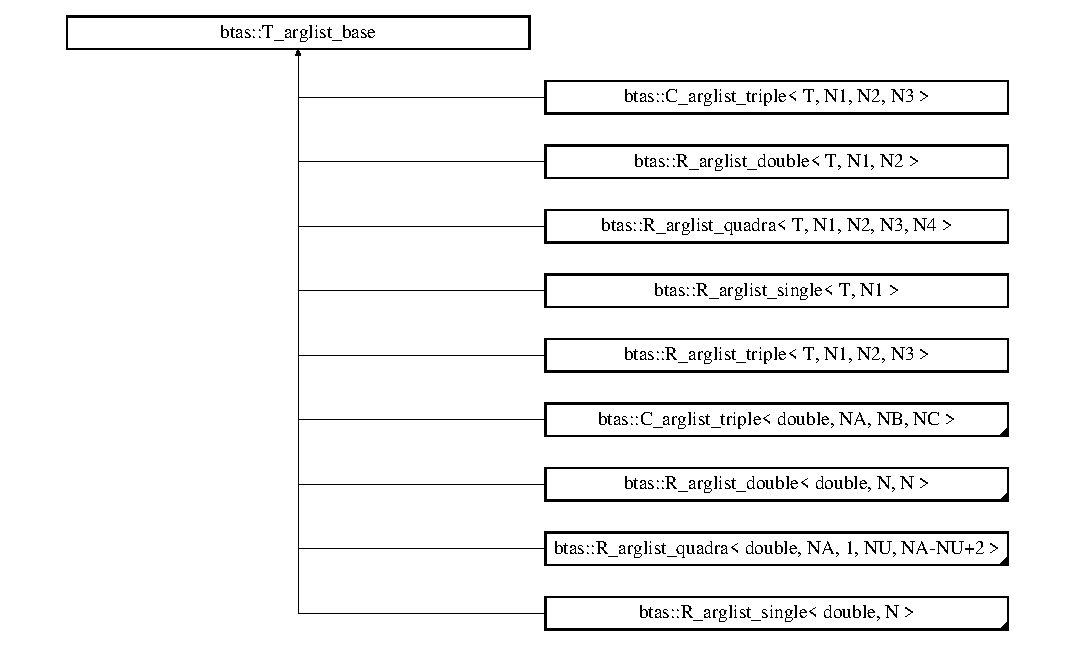
\includegraphics[height=8.235294cm]{d7/dd4/classbtas_1_1T__arglist__base}
\end{center}
\end{figure}
\subsection*{Public Member Functions}
\begin{DoxyCompactItemize}
\item 
{\bf T\-\_\-arglist\-\_\-base} (size\-\_\-t flops=0)
\begin{DoxyCompactList}\small\item\em Default constructor. \end{DoxyCompactList}\item 
virtual {\bf $\sim$\-T\-\_\-arglist\-\_\-base} ()
\begin{DoxyCompactList}\small\item\em Destructor. \end{DoxyCompactList}\item 
bool {\bf operator==} (const {\bf T\-\_\-arglist\-\_\-base} \&other) const 
\begin{DoxyCompactList}\small\item\em Boolian operator== for compare F\-L\-O\-P\-S count. \end{DoxyCompactList}\item 
bool {\bf operator!=} (const {\bf T\-\_\-arglist\-\_\-base} \&other) const 
\begin{DoxyCompactList}\small\item\em Boolian operator!= for compare F\-L\-O\-P\-S count. \end{DoxyCompactList}\item 
bool {\bf operator$<$} (const {\bf T\-\_\-arglist\-\_\-base} \&other) const 
\begin{DoxyCompactList}\small\item\em Boolian operator$<$ for sorting F\-L\-O\-P\-S count. \end{DoxyCompactList}\item 
bool {\bf operator$>$} (const {\bf T\-\_\-arglist\-\_\-base} \&other) const 
\begin{DoxyCompactList}\small\item\em Boolian operator$>$ for sorting F\-L\-O\-P\-S count. \end{DoxyCompactList}\end{DoxyCompactItemize}
\subsection*{Protected Attributes}
\begin{DoxyCompactItemize}
\item 
size\-\_\-t {\bf m\-\_\-flops}
\begin{DoxyCompactList}\small\item\em F\-L\-O\-P\-S count (aprox.) for load-\/balancing. \end{DoxyCompactList}\end{DoxyCompactItemize}


\subsection{Detailed Description}
Base class of argment list. 

This class is designed for shared-\/memory parallelization of sparse-\/array computations giving load-\/balancing functions

T\-O\-D\-O\-: For another design, call() might be implemented as pure-\/virtual function to carry out array computation 

Definition at line 28 of file Targlist.\-h.



\subsection{Constructor \& Destructor Documentation}
\index{btas\-::\-T\-\_\-arglist\-\_\-base@{btas\-::\-T\-\_\-arglist\-\_\-base}!T\-\_\-arglist\-\_\-base@{T\-\_\-arglist\-\_\-base}}
\index{T\-\_\-arglist\-\_\-base@{T\-\_\-arglist\-\_\-base}!btas::T_arglist_base@{btas\-::\-T\-\_\-arglist\-\_\-base}}
\subsubsection[{T\-\_\-arglist\-\_\-base}]{\setlength{\rightskip}{0pt plus 5cm}btas\-::\-T\-\_\-arglist\-\_\-base\-::\-T\-\_\-arglist\-\_\-base (
\begin{DoxyParamCaption}
\item[{size\-\_\-t}]{flops = {\ttfamily 0}}
\end{DoxyParamCaption}
)\hspace{0.3cm}{\ttfamily [inline]}}\label{d7/dd4/classbtas_1_1T__arglist__base_a0e424856c33471eea34cc47d24218e30}


Default constructor. 



Definition at line 34 of file Targlist.\-h.

\index{btas\-::\-T\-\_\-arglist\-\_\-base@{btas\-::\-T\-\_\-arglist\-\_\-base}!$\sim$\-T\-\_\-arglist\-\_\-base@{$\sim$\-T\-\_\-arglist\-\_\-base}}
\index{$\sim$\-T\-\_\-arglist\-\_\-base@{$\sim$\-T\-\_\-arglist\-\_\-base}!btas::T_arglist_base@{btas\-::\-T\-\_\-arglist\-\_\-base}}
\subsubsection[{$\sim$\-T\-\_\-arglist\-\_\-base}]{\setlength{\rightskip}{0pt plus 5cm}virtual btas\-::\-T\-\_\-arglist\-\_\-base\-::$\sim$\-T\-\_\-arglist\-\_\-base (
\begin{DoxyParamCaption}
{}
\end{DoxyParamCaption}
)\hspace{0.3cm}{\ttfamily [inline]}, {\ttfamily [virtual]}}\label{d7/dd4/classbtas_1_1T__arglist__base_ab89b427fb077cc6bfe1860919e939592}


Destructor. 



Definition at line 36 of file Targlist.\-h.



\subsection{Member Function Documentation}
\index{btas\-::\-T\-\_\-arglist\-\_\-base@{btas\-::\-T\-\_\-arglist\-\_\-base}!operator!=@{operator!=}}
\index{operator!=@{operator!=}!btas::T_arglist_base@{btas\-::\-T\-\_\-arglist\-\_\-base}}
\subsubsection[{operator!=}]{\setlength{\rightskip}{0pt plus 5cm}bool btas\-::\-T\-\_\-arglist\-\_\-base\-::operator!= (
\begin{DoxyParamCaption}
\item[{const {\bf T\-\_\-arglist\-\_\-base} \&}]{other}
\end{DoxyParamCaption}
) const\hspace{0.3cm}{\ttfamily [inline]}}\label{d7/dd4/classbtas_1_1T__arglist__base_a3a08de7ad4fcc2a0f5d5309743c58d9c}


Boolian operator!= for compare F\-L\-O\-P\-S count. 



Definition at line 40 of file Targlist.\-h.



References m\-\_\-flops.

\index{btas\-::\-T\-\_\-arglist\-\_\-base@{btas\-::\-T\-\_\-arglist\-\_\-base}!operator$<$@{operator$<$}}
\index{operator$<$@{operator$<$}!btas::T_arglist_base@{btas\-::\-T\-\_\-arglist\-\_\-base}}
\subsubsection[{operator$<$}]{\setlength{\rightskip}{0pt plus 5cm}bool btas\-::\-T\-\_\-arglist\-\_\-base\-::operator$<$ (
\begin{DoxyParamCaption}
\item[{const {\bf T\-\_\-arglist\-\_\-base} \&}]{other}
\end{DoxyParamCaption}
) const\hspace{0.3cm}{\ttfamily [inline]}}\label{d7/dd4/classbtas_1_1T__arglist__base_a6de9e8b71416d2710966aff70f7b5bf5}


Boolian operator$<$ for sorting F\-L\-O\-P\-S count. 



Definition at line 42 of file Targlist.\-h.



References m\-\_\-flops.

\index{btas\-::\-T\-\_\-arglist\-\_\-base@{btas\-::\-T\-\_\-arglist\-\_\-base}!operator==@{operator==}}
\index{operator==@{operator==}!btas::T_arglist_base@{btas\-::\-T\-\_\-arglist\-\_\-base}}
\subsubsection[{operator==}]{\setlength{\rightskip}{0pt plus 5cm}bool btas\-::\-T\-\_\-arglist\-\_\-base\-::operator== (
\begin{DoxyParamCaption}
\item[{const {\bf T\-\_\-arglist\-\_\-base} \&}]{other}
\end{DoxyParamCaption}
) const\hspace{0.3cm}{\ttfamily [inline]}}\label{d7/dd4/classbtas_1_1T__arglist__base_ac623c451d3ecffb91786e67140a1f5da}


Boolian operator== for compare F\-L\-O\-P\-S count. 



Definition at line 38 of file Targlist.\-h.



References m\-\_\-flops.

\index{btas\-::\-T\-\_\-arglist\-\_\-base@{btas\-::\-T\-\_\-arglist\-\_\-base}!operator$>$@{operator$>$}}
\index{operator$>$@{operator$>$}!btas::T_arglist_base@{btas\-::\-T\-\_\-arglist\-\_\-base}}
\subsubsection[{operator$>$}]{\setlength{\rightskip}{0pt plus 5cm}bool btas\-::\-T\-\_\-arglist\-\_\-base\-::operator$>$ (
\begin{DoxyParamCaption}
\item[{const {\bf T\-\_\-arglist\-\_\-base} \&}]{other}
\end{DoxyParamCaption}
) const\hspace{0.3cm}{\ttfamily [inline]}}\label{d7/dd4/classbtas_1_1T__arglist__base_a2ddd12126dfd4654d7648e60af965d9d}


Boolian operator$>$ for sorting F\-L\-O\-P\-S count. 



Definition at line 44 of file Targlist.\-h.



References m\-\_\-flops.



\subsection{Field Documentation}
\index{btas\-::\-T\-\_\-arglist\-\_\-base@{btas\-::\-T\-\_\-arglist\-\_\-base}!m\-\_\-flops@{m\-\_\-flops}}
\index{m\-\_\-flops@{m\-\_\-flops}!btas::T_arglist_base@{btas\-::\-T\-\_\-arglist\-\_\-base}}
\subsubsection[{m\-\_\-flops}]{\setlength{\rightskip}{0pt plus 5cm}size\-\_\-t btas\-::\-T\-\_\-arglist\-\_\-base\-::m\-\_\-flops\hspace{0.3cm}{\ttfamily [protected]}}\label{d7/dd4/classbtas_1_1T__arglist__base_aa1331e5b0a9e296c7648385efcf7ad45}


F\-L\-O\-P\-S count (aprox.) for load-\/balancing. 



Definition at line 31 of file Targlist.\-h.



Referenced by btas\-::\-C\-\_\-arglist\-\_\-triple$<$ double, N\-A, N\-B, N\-C $>$\-::add(), btas\-::\-C\-\_\-arglist\-\_\-triple$<$ double, N\-A, N\-B, N\-C $>$\-::clear(), operator!=(), operator$<$(), operator==(), operator$>$(), btas\-::\-R\-\_\-arglist\-\_\-double$<$ double, N, N $>$\-::\-R\-\_\-arglist\-\_\-double(), btas\-::\-R\-\_\-arglist\-\_\-quadra$<$ double, N\-A, 1, N\-U, N\-A-\/\-N\-U+2 $>$\-::\-R\-\_\-arglist\-\_\-quadra(), btas\-::\-R\-\_\-arglist\-\_\-single$<$ double, N $>$\-::\-R\-\_\-arglist\-\_\-single(), btas\-::\-R\-\_\-arglist\-\_\-triple$<$ T, N1, N2, N3 $>$\-::\-R\-\_\-arglist\-\_\-triple(), btas\-::\-R\-\_\-arglist\-\_\-single$<$ double, N $>$\-::reset(), btas\-::\-R\-\_\-arglist\-\_\-double$<$ double, N, N $>$\-::reset(), btas\-::\-R\-\_\-arglist\-\_\-triple$<$ T, N1, N2, N3 $>$\-::reset(), and btas\-::\-R\-\_\-arglist\-\_\-quadra$<$ double, N\-A, 1, N\-U, N\-A-\/\-N\-U+2 $>$\-::reset().



The documentation for this class was generated from the following file\-:\begin{DoxyCompactItemize}
\item 
include/btas/{\bf Targlist.\-h}\end{DoxyCompactItemize}

\section{btas\-:\-:T\-Array$<$ T, N $>$ Class Template Reference}
\label{db/d3c/classbtas_1_1TArray}\index{btas\-::\-T\-Array$<$ T, N $>$@{btas\-::\-T\-Array$<$ T, N $>$}}


Dense array class.  




{\ttfamily \#include $<$T\-Array.\-h$>$}

Inheritance diagram for btas\-:\-:T\-Array$<$ T, N $>$\-:\begin{figure}[H]
\begin{center}
\leavevmode
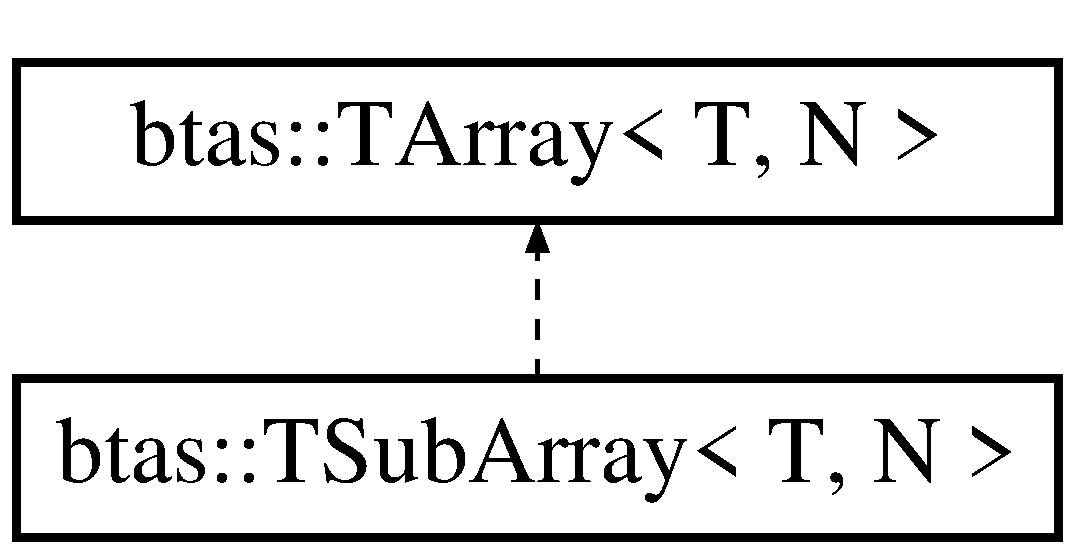
\includegraphics[height=2.000000cm]{db/d3c/classbtas_1_1TArray}
\end{center}
\end{figure}
\subsection*{Public Types}
\begin{DoxyCompactItemize}
\item 
typedef std\-::vector$<$ T $>$\-::{\bf iterator} {\bf iterator}
\begin{DoxyCompactList}\small\item\em \doxyref{T\-Array$<$\-T, N$>$\-::iterator}{p.}{db/d3c/classbtas_1_1TArray_ad5e17e7428d2ca293addf9e652ec477c}. \end{DoxyCompactList}\item 
typedef std\-::vector$<$ T $>$\\*
\-::{\bf const\-\_\-iterator} {\bf const\-\_\-iterator}
\begin{DoxyCompactList}\small\item\em \doxyref{T\-Array$<$\-T, N$>$\-::const\-\_\-iterator}{p.}{db/d3c/classbtas_1_1TArray_afc4622d214e7ced620c448a5d0574ac8}. \end{DoxyCompactList}\end{DoxyCompactItemize}
\subsection*{Public Member Functions}
\begin{DoxyCompactItemize}
\item 
{\bf T\-Array} ()
\begin{DoxyCompactList}\small\item\em default constructor \end{DoxyCompactList}\item 
{\bf $\sim$\-T\-Array} ()
\begin{DoxyCompactList}\small\item\em destructor \end{DoxyCompactList}\item 
{\bf T\-Array} (const {\bf T\-Array} \&other)
\begin{DoxyCompactList}\small\item\em copy constructor \end{DoxyCompactList}\item 
{\bf T\-Array} \& {\bf operator=} (const {\bf T\-Array} \&other)
\begin{DoxyCompactList}\small\item\em copy assignment operator \end{DoxyCompactList}\item 
{\bf T\-Array} \& {\bf operator+=} (const {\bf T\-Array} \&other)
\begin{DoxyCompactList}\small\item\em addition assignment operator \end{DoxyCompactList}\item 
void {\bf copy} (const {\bf T\-Array} \&other)
\begin{DoxyCompactList}\small\item\em copying from other to this \end{DoxyCompactList}\item 
{\bf T\-Array} {\bf copy} () const 
\begin{DoxyCompactList}\small\item\em return copy of this \end{DoxyCompactList}\item 
{\footnotesize template$<$size\-\_\-t M$>$ }\\void {\bf copy} (const {\bf T\-Sub\-Array}$<$ T, M $>$ \&a)
\begin{DoxyCompactList}\small\item\em Copy from sub-\/array to array. \end{DoxyCompactList}\item 
void {\bf scale} (const T \&alpha)
\begin{DoxyCompactList}\small\item\em scale by const value \end{DoxyCompactList}\item 
void {\bf add} (const {\bf T\-Array} \&other)
\begin{DoxyCompactList}\small\item\em adding from other to this \end{DoxyCompactList}\item 
{\footnotesize template$<$size\-\_\-t M$>$ }\\{\bf T\-Array} (const {\bf T\-Sub\-Array}$<$ T, M $>$ \&sub)
\begin{DoxyCompactList}\small\item\em copy constructor from sub-\/array \end{DoxyCompactList}\item 
{\footnotesize template$<$size\-\_\-t M$>$ }\\{\bf T\-Array} \& {\bf operator=} (const {\bf T\-Sub\-Array}$<$ T, M $>$ \&sub)
\begin{DoxyCompactList}\small\item\em copy assignment from sub-\/array \end{DoxyCompactList}\item 
{\bf T\-Array} ({\bf T\-Array} \&\&other)
\begin{DoxyCompactList}\small\item\em move constructor \end{DoxyCompactList}\item 
{\bf T\-Array} \& {\bf operator=} ({\bf T\-Array} \&\&other)
\begin{DoxyCompactList}\small\item\em move assignment \end{DoxyCompactList}\item 
void {\bf reference} (const {\bf T\-Array} \&other)
\begin{DoxyCompactList}\small\item\em take data reference from other \end{DoxyCompactList}\item 
{\bf T\-Array} {\bf reference} () const 
\begin{DoxyCompactList}\small\item\em return data reference of this \end{DoxyCompactList}\item 
{\bf T\-Array} (int n01)
\begin{DoxyCompactList}\small\item\em convenient constructor with array shape, for N = 1 \end{DoxyCompactList}\item 
{\bf T\-Array} (int n01, int n02)
\begin{DoxyCompactList}\small\item\em convenient constructor with array shape, for N = 2 \end{DoxyCompactList}\item 
{\bf T\-Array} (int n01, int n02, int n03)
\begin{DoxyCompactList}\small\item\em convenient constructor with array shape, for N = 3 \end{DoxyCompactList}\item 
{\bf T\-Array} (int n01, int n02, int n03, int n04)
\begin{DoxyCompactList}\small\item\em convenient constructor with array shape, for N = 4 \end{DoxyCompactList}\item 
{\bf T\-Array} (int n01, int n02, int n03, int n04, int n05)
\begin{DoxyCompactList}\small\item\em convenient constructor with array shape, for N = 5 \end{DoxyCompactList}\item 
{\bf T\-Array} (int n01, int n02, int n03, int n04, int n05, int n06)
\begin{DoxyCompactList}\small\item\em convenient constructor with array shape, for N = 6 \end{DoxyCompactList}\item 
{\bf T\-Array} (int n01, int n02, int n03, int n04, int n05, int n06, int n07)
\begin{DoxyCompactList}\small\item\em convenient constructor with array shape, for N = 7 \end{DoxyCompactList}\item 
{\bf T\-Array} (int n01, int n02, int n03, int n04, int n05, int n06, int n07, int n08)
\begin{DoxyCompactList}\small\item\em convenient constructor with array shape, for N = 8 \end{DoxyCompactList}\item 
{\bf T\-Array} (int n01, int n02, int n03, int n04, int n05, int n06, int n07, int n08, int n09)
\begin{DoxyCompactList}\small\item\em convenient constructor with array shape, for N = 9 \end{DoxyCompactList}\item 
{\bf T\-Array} (int n01, int n02, int n03, int n04, int n05, int n06, int n07, int n08, int n09, int n10)
\begin{DoxyCompactList}\small\item\em convenient constructor with array shape, for N = 10 \end{DoxyCompactList}\item 
{\bf T\-Array} (int n01, int n02, int n03, int n04, int n05, int n06, int n07, int n08, int n09, int n10, int n11)
\begin{DoxyCompactList}\small\item\em convenient constructor with array shape, for N = 11 \end{DoxyCompactList}\item 
{\bf T\-Array} (int n01, int n02, int n03, int n04, int n05, int n06, int n07, int n08, int n09, int n10, int n11, int n12)
\begin{DoxyCompactList}\small\item\em convenient constructor with array shape, for N = 12 \end{DoxyCompactList}\item 
{\bf T\-Array} (const {\bf I\-Vector}$<$ N $>$ \&\-\_\-shape)
\begin{DoxyCompactList}\small\item\em convenient constructor with array shape, for arbitrary N \end{DoxyCompactList}\item 
void {\bf resize} (int n01)
\begin{DoxyCompactList}\small\item\em resize array shape, for N = 1 \end{DoxyCompactList}\item 
void {\bf resize} (int n01, int n02)
\begin{DoxyCompactList}\small\item\em resize array shape, for N = 2 \end{DoxyCompactList}\item 
void {\bf resize} (int n01, int n02, int n03)
\begin{DoxyCompactList}\small\item\em resize array shape, for N = 3 \end{DoxyCompactList}\item 
void {\bf resize} (int n01, int n02, int n03, int n04)
\begin{DoxyCompactList}\small\item\em resize array shape, for N = 4 \end{DoxyCompactList}\item 
void {\bf resize} (int n01, int n02, int n03, int n04, int n05)
\begin{DoxyCompactList}\small\item\em resize array shape, for N = 5 \end{DoxyCompactList}\item 
void {\bf resize} (int n01, int n02, int n03, int n04, int n05, int n06)
\begin{DoxyCompactList}\small\item\em resize array shape, for N = 6 \end{DoxyCompactList}\item 
void {\bf resize} (int n01, int n02, int n03, int n04, int n05, int n06, int n07)
\begin{DoxyCompactList}\small\item\em resize array shape, for N = 7 \end{DoxyCompactList}\item 
void {\bf resize} (int n01, int n02, int n03, int n04, int n05, int n06, int n07, int n08)
\begin{DoxyCompactList}\small\item\em resize array shape, for N = 8 \end{DoxyCompactList}\item 
void {\bf resize} (int n01, int n02, int n03, int n04, int n05, int n06, int n07, int n08, int n09)
\begin{DoxyCompactList}\small\item\em resize array shape, for N = 9 \end{DoxyCompactList}\item 
void {\bf resize} (int n01, int n02, int n03, int n04, int n05, int n06, int n07, int n08, int n09, int n10)
\begin{DoxyCompactList}\small\item\em resize array shape, for N = 10 \end{DoxyCompactList}\item 
void {\bf resize} (int n01, int n02, int n03, int n04, int n05, int n06, int n07, int n08, int n09, int n10, int n11)
\begin{DoxyCompactList}\small\item\em resize array shape, for N = 11 \end{DoxyCompactList}\item 
void {\bf resize} (int n01, int n02, int n03, int n04, int n05, int n06, int n07, int n08, int n09, int n10, int n11, int n12)
\begin{DoxyCompactList}\small\item\em resize array shape, for N = 12 \end{DoxyCompactList}\item 
void {\bf resize} (const {\bf I\-Vector}$<$ N $>$ \&\-\_\-shape)
\begin{DoxyCompactList}\small\item\em resize array by \-\_\-shape, for arbitrary N \end{DoxyCompactList}\item 
{\bf const\-\_\-iterator} {\bf begin} () const 
\begin{DoxyCompactList}\small\item\em returns first iterator position (const) \end{DoxyCompactList}\item 
{\bf iterator} {\bf begin} ()
\begin{DoxyCompactList}\small\item\em returns first iterator position \end{DoxyCompactList}\item 
{\bf const\-\_\-iterator} {\bf end} () const 
\begin{DoxyCompactList}\small\item\em returns last iterator position (const) \end{DoxyCompactList}\item 
{\bf iterator} {\bf end} ()
\begin{DoxyCompactList}\small\item\em returns last iterator position \end{DoxyCompactList}\item 
const {\bf I\-Vector}$<$ N $>$ \& {\bf shape} () const 
\begin{DoxyCompactList}\small\item\em returns array shape \end{DoxyCompactList}\item 
int {\bf shape} (int i) const 
\begin{DoxyCompactList}\small\item\em returns array shape for rank i \end{DoxyCompactList}\item 
const {\bf I\-Vector}$<$ N $>$ \& {\bf stride} () const 
\begin{DoxyCompactList}\small\item\em returns array stride \end{DoxyCompactList}\item 
int {\bf stride} (int i) const 
\begin{DoxyCompactList}\small\item\em returns array stride for rank i \end{DoxyCompactList}\item 
size\-\_\-t {\bf size} () const 
\begin{DoxyCompactList}\small\item\em returns allocated size \end{DoxyCompactList}\item 
const T \& {\bf operator()} (int i01) const 
\begin{DoxyCompactList}\small\item\em returns array element (N = 1) without range check \end{DoxyCompactList}\item 
const T \& {\bf operator()} (int i01, int i02) const 
\begin{DoxyCompactList}\small\item\em returns array element (N = 2) without range check \end{DoxyCompactList}\item 
const T \& {\bf operator()} (int i01, int i02, int i03) const 
\begin{DoxyCompactList}\small\item\em returns array element (N = 3) without range check \end{DoxyCompactList}\item 
const T \& {\bf operator()} (int i01, int i02, int i03, int i04) const 
\begin{DoxyCompactList}\small\item\em returns array element (N = 4) without range check \end{DoxyCompactList}\item 
const T \& {\bf operator()} (int i01, int i02, int i03, int i04, int i05) const 
\begin{DoxyCompactList}\small\item\em returns array element (N = 5) without range check \end{DoxyCompactList}\item 
const T \& {\bf operator()} (int i01, int i02, int i03, int i04, int i05, int i06) const 
\begin{DoxyCompactList}\small\item\em returns array element (N = 6) without range check \end{DoxyCompactList}\item 
const T \& {\bf operator()} (int i01, int i02, int i03, int i04, int i05, int i06, int i07) const 
\begin{DoxyCompactList}\small\item\em returns array element (N = 7) without range check \end{DoxyCompactList}\item 
const T \& {\bf operator()} (int i01, int i02, int i03, int i04, int i05, int i06, int i07, int i08) const 
\begin{DoxyCompactList}\small\item\em returns array element (N = 8) without range check \end{DoxyCompactList}\item 
const T \& {\bf operator()} (int i01, int i02, int i03, int i04, int i05, int i06, int i07, int i08, int i09) const 
\begin{DoxyCompactList}\small\item\em returns array element (N = 9) without range check \end{DoxyCompactList}\item 
const T \& {\bf operator()} (int i01, int i02, int i03, int i04, int i05, int i06, int i07, int i08, int i09, int i10) const 
\begin{DoxyCompactList}\small\item\em returns array element (N = 10) without range check \end{DoxyCompactList}\item 
const T \& {\bf operator()} (int i01, int i02, int i03, int i04, int i05, int i06, int i07, int i08, int i09, int i10, int i11) const 
\begin{DoxyCompactList}\small\item\em returns array element (N = 11) without range check \end{DoxyCompactList}\item 
const T \& {\bf operator()} (int i01, int i02, int i03, int i04, int i05, int i06, int i07, int i08, int i09, int i10, int i11, int i12) const 
\begin{DoxyCompactList}\small\item\em returns array element (N = 12) without range check \end{DoxyCompactList}\item 
const T \& {\bf operator()} (const {\bf I\-Vector}$<$ N $>$ \&\-\_\-index) const 
\begin{DoxyCompactList}\small\item\em returns array element (arbitrary N) without range check \end{DoxyCompactList}\item 
T \& {\bf operator()} (int i01)
\begin{DoxyCompactList}\small\item\em returns array element (N = 1) without range check \end{DoxyCompactList}\item 
T \& {\bf operator()} (int i01, int i02)
\begin{DoxyCompactList}\small\item\em returns array element (N = 2) without range check \end{DoxyCompactList}\item 
T \& {\bf operator()} (int i01, int i02, int i03)
\begin{DoxyCompactList}\small\item\em returns array element (N = 3) without range check \end{DoxyCompactList}\item 
T \& {\bf operator()} (int i01, int i02, int i03, int i04)
\begin{DoxyCompactList}\small\item\em returns array element (N = 4) without range check \end{DoxyCompactList}\item 
T \& {\bf operator()} (int i01, int i02, int i03, int i04, int i05)
\begin{DoxyCompactList}\small\item\em returns array element (N = 5) without range check \end{DoxyCompactList}\item 
T \& {\bf operator()} (int i01, int i02, int i03, int i04, int i05, int i06)
\begin{DoxyCompactList}\small\item\em returns array element (N = 6) without range check \end{DoxyCompactList}\item 
T \& {\bf operator()} (int i01, int i02, int i03, int i04, int i05, int i06, int i07)
\begin{DoxyCompactList}\small\item\em returns array element (N = 7) without range check \end{DoxyCompactList}\item 
T \& {\bf operator()} (int i01, int i02, int i03, int i04, int i05, int i06, int i07, int i08)
\begin{DoxyCompactList}\small\item\em returns array element (N = 8) without range check \end{DoxyCompactList}\item 
T \& {\bf operator()} (int i01, int i02, int i03, int i04, int i05, int i06, int i07, int i08, int i09)
\begin{DoxyCompactList}\small\item\em returns array element (N = 9) without range check \end{DoxyCompactList}\item 
T \& {\bf operator()} (int i01, int i02, int i03, int i04, int i05, int i06, int i07, int i08, int i09, int i10)
\begin{DoxyCompactList}\small\item\em returns array element (N = 10) without range check \end{DoxyCompactList}\item 
T \& {\bf operator()} (int i01, int i02, int i03, int i04, int i05, int i06, int i07, int i08, int i09, int i10, int i11)
\begin{DoxyCompactList}\small\item\em returns array element (N = 11) without range check \end{DoxyCompactList}\item 
T \& {\bf operator()} (int i01, int i02, int i03, int i04, int i05, int i06, int i07, int i08, int i09, int i10, int i11, int i12)
\begin{DoxyCompactList}\small\item\em returns array element (N = 12) without range check \end{DoxyCompactList}\item 
T \& {\bf operator()} (const {\bf I\-Vector}$<$ N $>$ \&\-\_\-index)
\begin{DoxyCompactList}\small\item\em returns array element (arbitrary N) without range check \end{DoxyCompactList}\item 
const T \& {\bf at} (int i01) const 
\begin{DoxyCompactList}\small\item\em returns array element (N = 1) with range check \end{DoxyCompactList}\item 
const T \& {\bf at} (int i01, int i02) const 
\begin{DoxyCompactList}\small\item\em returns array element (N = 2) with range check \end{DoxyCompactList}\item 
const T \& {\bf at} (int i01, int i02, int i03) const 
\begin{DoxyCompactList}\small\item\em returns array element (N = 3) with range check \end{DoxyCompactList}\item 
const T \& {\bf at} (int i01, int i02, int i03, int i04) const 
\begin{DoxyCompactList}\small\item\em returns array element (N = 4) with range check \end{DoxyCompactList}\item 
const T \& {\bf at} (int i01, int i02, int i03, int i04, int i05) const 
\begin{DoxyCompactList}\small\item\em returns array element (N = 5) with range check \end{DoxyCompactList}\item 
const T \& {\bf at} (int i01, int i02, int i03, int i04, int i05, int i06) const 
\begin{DoxyCompactList}\small\item\em returns array element (N = 6) with range check \end{DoxyCompactList}\item 
const T \& {\bf at} (int i01, int i02, int i03, int i04, int i05, int i06, int i07) const 
\begin{DoxyCompactList}\small\item\em returns array element (N = 7) with range check \end{DoxyCompactList}\item 
const T \& {\bf at} (int i01, int i02, int i03, int i04, int i05, int i06, int i07, int i08) const 
\begin{DoxyCompactList}\small\item\em returns array element (N = 8) with range check \end{DoxyCompactList}\item 
const T \& {\bf at} (int i01, int i02, int i03, int i04, int i05, int i06, int i07, int i08, int i09) const 
\begin{DoxyCompactList}\small\item\em returns array element (N = 9) with range check \end{DoxyCompactList}\item 
const T \& {\bf at} (int i01, int i02, int i03, int i04, int i05, int i06, int i07, int i08, int i09, int i10) const 
\begin{DoxyCompactList}\small\item\em returns array element (N = 10) with range check \end{DoxyCompactList}\item 
const T \& {\bf at} (int i01, int i02, int i03, int i04, int i05, int i06, int i07, int i08, int i09, int i10, int i11) const 
\begin{DoxyCompactList}\small\item\em returns array element (N = 11) with range check \end{DoxyCompactList}\item 
const T \& {\bf at} (int i01, int i02, int i03, int i04, int i05, int i06, int i07, int i08, int i09, int i10, int i11, int i12) const 
\begin{DoxyCompactList}\small\item\em returns array element (N = 12) with range check \end{DoxyCompactList}\item 
const T \& {\bf at} (const {\bf I\-Vector}$<$ N $>$ \&\-\_\-index) const 
\begin{DoxyCompactList}\small\item\em returns array element (arbitrary N) with range check \end{DoxyCompactList}\item 
T \& {\bf at} (int i01)
\begin{DoxyCompactList}\small\item\em returns array element (N = 1) with range check \end{DoxyCompactList}\item 
T \& {\bf at} (int i01, int i02)
\begin{DoxyCompactList}\small\item\em returns array element (N = 2) with range check \end{DoxyCompactList}\item 
T \& {\bf at} (int i01, int i02, int i03)
\begin{DoxyCompactList}\small\item\em returns array element (N = 3) with range check \end{DoxyCompactList}\item 
T \& {\bf at} (int i01, int i02, int i03, int i04)
\begin{DoxyCompactList}\small\item\em returns array element (N = 4) with range check \end{DoxyCompactList}\item 
T \& {\bf at} (int i01, int i02, int i03, int i04, int i05)
\begin{DoxyCompactList}\small\item\em returns array element (N = 5) with range check \end{DoxyCompactList}\item 
T \& {\bf at} (int i01, int i02, int i03, int i04, int i05, int i06)
\begin{DoxyCompactList}\small\item\em returns array element (N = 6) with range check \end{DoxyCompactList}\item 
T \& {\bf at} (int i01, int i02, int i03, int i04, int i05, int i06, int i07)
\begin{DoxyCompactList}\small\item\em returns array element (N = 7) with range check \end{DoxyCompactList}\item 
T \& {\bf at} (int i01, int i02, int i03, int i04, int i05, int i06, int i07, int i08)
\begin{DoxyCompactList}\small\item\em returns array element (N = 8) with range check \end{DoxyCompactList}\item 
T \& {\bf at} (int i01, int i02, int i03, int i04, int i05, int i06, int i07, int i08, int i09)
\begin{DoxyCompactList}\small\item\em returns array element (N = 9) with range check \end{DoxyCompactList}\item 
T \& {\bf at} (int i01, int i02, int i03, int i04, int i05, int i06, int i07, int i08, int i09, int i10)
\begin{DoxyCompactList}\small\item\em returns array element (N = 10) with range check \end{DoxyCompactList}\item 
T \& {\bf at} (int i01, int i02, int i03, int i04, int i05, int i06, int i07, int i08, int i09, int i10, int i11)
\begin{DoxyCompactList}\small\item\em returns array element (N = 11) with range check \end{DoxyCompactList}\item 
T \& {\bf at} (int i01, int i02, int i03, int i04, int i05, int i06, int i07, int i08, int i09, int i10, int i11, int i12)
\begin{DoxyCompactList}\small\item\em returns array element (N = 12) with range check \end{DoxyCompactList}\item 
T \& {\bf at} (const {\bf I\-Vector}$<$ N $>$ \&\-\_\-index)
\begin{DoxyCompactList}\small\item\em returns array element (arbitrary N) with range check \end{DoxyCompactList}\item 
{\bf T\-Sub\-Array}$<$ T, N $>$ {\bf subarray} (const {\bf I\-Vector}$<$ N $>$ \&lbound, const {\bf I\-Vector}$<$ N $>$ \&ubound) const 
\begin{DoxyCompactList}\small\item\em slice array to return sub-\/array object \end{DoxyCompactList}\item 
const T $\ast$ {\bf data} () const 
\begin{DoxyCompactList}\small\item\em returns the first pointer of array elements \end{DoxyCompactList}\item 
T $\ast$ {\bf data} ()
\begin{DoxyCompactList}\small\item\em returns the first pointer of array elements \end{DoxyCompactList}\item 
void {\bf fill} (const T \&val)
\begin{DoxyCompactList}\small\item\em fills elements by constant value \end{DoxyCompactList}\item 
void {\bf operator=} (const T \&val)
\begin{DoxyCompactList}\small\item\em fills elements by constant value \end{DoxyCompactList}\item 
{\footnotesize template$<$class Generator $>$ }\\void {\bf generate} (Generator gen)
\begin{DoxyCompactList}\small\item\em generates array elements by function gen \end{DoxyCompactList}\item 
void {\bf clear} ()
\begin{DoxyCompactList}\small\item\em deallocate storage \end{DoxyCompactList}\end{DoxyCompactItemize}
\subsection*{Private Member Functions}
\begin{DoxyCompactItemize}
\item 
{\footnotesize template$<$class Archive $>$ }\\void {\bf serialize} (Archive \&ar, const unsigned int version)
\begin{DoxyCompactList}\small\item\em Enables to use boost serialization. \end{DoxyCompactList}\end{DoxyCompactItemize}
\subsection*{Private Attributes}
\begin{DoxyCompactItemize}
\item 
{\bf I\-Vector}$<$ N $>$ {\bf m\-\_\-shape}
\begin{DoxyCompactList}\small\item\em array shape \end{DoxyCompactList}\item 
{\bf I\-Vector}$<$ N $>$ {\bf m\-\_\-stride}
\begin{DoxyCompactList}\small\item\em array stride \end{DoxyCompactList}\item 
shared\-\_\-ptr$<$ std\-::vector$<$ T $>$ $>$ {\bf m\-\_\-store}
\begin{DoxyCompactList}\small\item\em array storage \end{DoxyCompactList}\end{DoxyCompactItemize}
\subsection*{Friends}
\begin{DoxyCompactItemize}
\item 
class {\bf boost\-::serialization\-::access}
\item 
{\footnotesize template$<$typename U , size\-\_\-t M$>$ }\\class {\bf T\-Sub\-Array}
\begin{DoxyCompactList}\small\item\em Any \doxyref{T\-Sub\-Array}{p.}{da/d50/classbtas_1_1TSubArray} classes being friend of T\-Array$<$\-T, N$>$ \end{DoxyCompactList}\end{DoxyCompactItemize}


\subsection{Detailed Description}
\subsubsection*{template$<$typename T, size\-\_\-t N$>$class btas\-::\-T\-Array$<$ T, N $>$}

Dense array class. 

Fixed-\/rank array class implemented in terms of std\-::array and std\-::vector Since using C++11 features, not compatible for C++03 compiler


\begin{DoxyParams}{Parameters}
{\em T} & value type \\
\hline
{\em N} & array rank \\
\hline
\end{DoxyParams}


Definition at line 22 of file T\-Array.\-h.



\subsection{Member Typedef Documentation}
\index{btas\-::\-T\-Array@{btas\-::\-T\-Array}!const\-\_\-iterator@{const\-\_\-iterator}}
\index{const\-\_\-iterator@{const\-\_\-iterator}!btas::TArray@{btas\-::\-T\-Array}}
\subsubsection[{const\-\_\-iterator}]{\setlength{\rightskip}{0pt plus 5cm}template$<$typename T, size\-\_\-t N$>$ typedef std\-::vector$<$T$>$\-::{\bf const\-\_\-iterator} {\bf btas\-::\-T\-Array}$<$ T, N $>$\-::{\bf const\-\_\-iterator}}\label{db/d3c/classbtas_1_1TArray_afc4622d214e7ced620c448a5d0574ac8}


\doxyref{T\-Array$<$\-T, N$>$\-::const\-\_\-iterator}{p.}{db/d3c/classbtas_1_1TArray_afc4622d214e7ced620c448a5d0574ac8}. 



Definition at line 61 of file T\-Array.\-h.

\index{btas\-::\-T\-Array@{btas\-::\-T\-Array}!iterator@{iterator}}
\index{iterator@{iterator}!btas::TArray@{btas\-::\-T\-Array}}
\subsubsection[{iterator}]{\setlength{\rightskip}{0pt plus 5cm}template$<$typename T, size\-\_\-t N$>$ typedef std\-::vector$<$T$>$\-::{\bf iterator} {\bf btas\-::\-T\-Array}$<$ T, N $>$\-::{\bf iterator}}\label{db/d3c/classbtas_1_1TArray_ad5e17e7428d2ca293addf9e652ec477c}


\doxyref{T\-Array$<$\-T, N$>$\-::iterator}{p.}{db/d3c/classbtas_1_1TArray_ad5e17e7428d2ca293addf9e652ec477c}. 



Definition at line 58 of file T\-Array.\-h.



\subsection{Constructor \& Destructor Documentation}
\index{btas\-::\-T\-Array@{btas\-::\-T\-Array}!T\-Array@{T\-Array}}
\index{T\-Array@{T\-Array}!btas::TArray@{btas\-::\-T\-Array}}
\subsubsection[{T\-Array}]{\setlength{\rightskip}{0pt plus 5cm}template$<$typename T, size\-\_\-t N$>$ {\bf btas\-::\-T\-Array}$<$ T, N $>$\-::{\bf T\-Array} (
\begin{DoxyParamCaption}
{}
\end{DoxyParamCaption}
)\hspace{0.3cm}{\ttfamily [inline]}}\label{db/d3c/classbtas_1_1TArray_af3e669326c7d5689fd909b8f5d011b1a}


default constructor 



Definition at line 72 of file T\-Array.\-h.



References btas\-::\-T\-Array$<$ T, N $>$\-::m\-\_\-shape, and btas\-::\-T\-Array$<$ T, N $>$\-::m\-\_\-stride.

\index{btas\-::\-T\-Array@{btas\-::\-T\-Array}!$\sim$\-T\-Array@{$\sim$\-T\-Array}}
\index{$\sim$\-T\-Array@{$\sim$\-T\-Array}!btas::TArray@{btas\-::\-T\-Array}}
\subsubsection[{$\sim$\-T\-Array}]{\setlength{\rightskip}{0pt plus 5cm}template$<$typename T, size\-\_\-t N$>$ {\bf btas\-::\-T\-Array}$<$ T, N $>$\-::$\sim${\bf T\-Array} (
\begin{DoxyParamCaption}
{}
\end{DoxyParamCaption}
)\hspace{0.3cm}{\ttfamily [inline]}}\label{db/d3c/classbtas_1_1TArray_a133b4d82d1ea55711dd8ca25e8113885}


destructor 



Definition at line 78 of file T\-Array.\-h.

\index{btas\-::\-T\-Array@{btas\-::\-T\-Array}!T\-Array@{T\-Array}}
\index{T\-Array@{T\-Array}!btas::TArray@{btas\-::\-T\-Array}}
\subsubsection[{T\-Array}]{\setlength{\rightskip}{0pt plus 5cm}template$<$typename T, size\-\_\-t N$>$ {\bf btas\-::\-T\-Array}$<$ T, N $>$\-::{\bf T\-Array} (
\begin{DoxyParamCaption}
\item[{const {\bf T\-Array}$<$ T, N $>$ \&}]{other}
\end{DoxyParamCaption}
)\hspace{0.3cm}{\ttfamily [inline]}, {\ttfamily [explicit]}}\label{db/d3c/classbtas_1_1TArray_abe5942e9f2464f5ad816f2e161ef29c6}


copy constructor 



Definition at line 81 of file T\-Array.\-h.



References btas\-::\-T\-Array$<$ T, N $>$\-::copy().

\index{btas\-::\-T\-Array@{btas\-::\-T\-Array}!T\-Array@{T\-Array}}
\index{T\-Array@{T\-Array}!btas::TArray@{btas\-::\-T\-Array}}
\subsubsection[{T\-Array}]{\setlength{\rightskip}{0pt plus 5cm}template$<$typename T, size\-\_\-t N$>$ template$<$size\-\_\-t M$>$ {\bf btas\-::\-T\-Array}$<$ T, N $>$\-::{\bf T\-Array} (
\begin{DoxyParamCaption}
\item[{const {\bf T\-Sub\-Array}$<$ T, M $>$ \&}]{sub}
\end{DoxyParamCaption}
)\hspace{0.3cm}{\ttfamily [inline]}, {\ttfamily [explicit]}}\label{db/d3c/classbtas_1_1TArray_a07313148cb759403443f0e292b43a233}


copy constructor from sub-\/array 



Definition at line 154 of file T\-Array.\-h.



References btas\-::\-T\-Array$<$ T, N $>$\-::copy().

\index{btas\-::\-T\-Array@{btas\-::\-T\-Array}!T\-Array@{T\-Array}}
\index{T\-Array@{T\-Array}!btas::TArray@{btas\-::\-T\-Array}}
\subsubsection[{T\-Array}]{\setlength{\rightskip}{0pt plus 5cm}template$<$typename T, size\-\_\-t N$>$ {\bf btas\-::\-T\-Array}$<$ T, N $>$\-::{\bf T\-Array} (
\begin{DoxyParamCaption}
\item[{{\bf T\-Array}$<$ T, N $>$ \&\&}]{other}
\end{DoxyParamCaption}
)\hspace{0.3cm}{\ttfamily [inline]}, {\ttfamily [explicit]}}\label{db/d3c/classbtas_1_1TArray_a47ddd792899a337276227e1fbe63c5a6}


move constructor 



Definition at line 166 of file T\-Array.\-h.

\index{btas\-::\-T\-Array@{btas\-::\-T\-Array}!T\-Array@{T\-Array}}
\index{T\-Array@{T\-Array}!btas::TArray@{btas\-::\-T\-Array}}
\subsubsection[{T\-Array}]{\setlength{\rightskip}{0pt plus 5cm}template$<$typename T, size\-\_\-t N$>$ {\bf btas\-::\-T\-Array}$<$ T, N $>$\-::{\bf T\-Array} (
\begin{DoxyParamCaption}
\item[{int}]{n01}
\end{DoxyParamCaption}
)\hspace{0.3cm}{\ttfamily [inline]}, {\ttfamily [explicit]}}\label{db/d3c/classbtas_1_1TArray_ac07050bcfdc09cb8b1f9842dd5cc032b}


convenient constructor with array shape, for N = 1 



Definition at line 192 of file T\-Array.\-h.



References btas\-::\-T\-Array$<$ T, N $>$\-::resize().

\index{btas\-::\-T\-Array@{btas\-::\-T\-Array}!T\-Array@{T\-Array}}
\index{T\-Array@{T\-Array}!btas::TArray@{btas\-::\-T\-Array}}
\subsubsection[{T\-Array}]{\setlength{\rightskip}{0pt plus 5cm}template$<$typename T, size\-\_\-t N$>$ {\bf btas\-::\-T\-Array}$<$ T, N $>$\-::{\bf T\-Array} (
\begin{DoxyParamCaption}
\item[{int}]{n01, }
\item[{int}]{n02}
\end{DoxyParamCaption}
)\hspace{0.3cm}{\ttfamily [inline]}}\label{db/d3c/classbtas_1_1TArray_a2fcde972162e07b02ca9b3db7f47233f}


convenient constructor with array shape, for N = 2 



Definition at line 197 of file T\-Array.\-h.



References btas\-::\-T\-Array$<$ T, N $>$\-::resize().

\index{btas\-::\-T\-Array@{btas\-::\-T\-Array}!T\-Array@{T\-Array}}
\index{T\-Array@{T\-Array}!btas::TArray@{btas\-::\-T\-Array}}
\subsubsection[{T\-Array}]{\setlength{\rightskip}{0pt plus 5cm}template$<$typename T, size\-\_\-t N$>$ {\bf btas\-::\-T\-Array}$<$ T, N $>$\-::{\bf T\-Array} (
\begin{DoxyParamCaption}
\item[{int}]{n01, }
\item[{int}]{n02, }
\item[{int}]{n03}
\end{DoxyParamCaption}
)\hspace{0.3cm}{\ttfamily [inline]}}\label{db/d3c/classbtas_1_1TArray_a725dea63f583dbc2241a7de91f0b831a}


convenient constructor with array shape, for N = 3 



Definition at line 202 of file T\-Array.\-h.



References btas\-::\-T\-Array$<$ T, N $>$\-::resize().

\index{btas\-::\-T\-Array@{btas\-::\-T\-Array}!T\-Array@{T\-Array}}
\index{T\-Array@{T\-Array}!btas::TArray@{btas\-::\-T\-Array}}
\subsubsection[{T\-Array}]{\setlength{\rightskip}{0pt plus 5cm}template$<$typename T, size\-\_\-t N$>$ {\bf btas\-::\-T\-Array}$<$ T, N $>$\-::{\bf T\-Array} (
\begin{DoxyParamCaption}
\item[{int}]{n01, }
\item[{int}]{n02, }
\item[{int}]{n03, }
\item[{int}]{n04}
\end{DoxyParamCaption}
)\hspace{0.3cm}{\ttfamily [inline]}}\label{db/d3c/classbtas_1_1TArray_a62f02eaeaed4ba260094f696f6127b48}


convenient constructor with array shape, for N = 4 



Definition at line 207 of file T\-Array.\-h.



References btas\-::\-T\-Array$<$ T, N $>$\-::resize().

\index{btas\-::\-T\-Array@{btas\-::\-T\-Array}!T\-Array@{T\-Array}}
\index{T\-Array@{T\-Array}!btas::TArray@{btas\-::\-T\-Array}}
\subsubsection[{T\-Array}]{\setlength{\rightskip}{0pt plus 5cm}template$<$typename T, size\-\_\-t N$>$ {\bf btas\-::\-T\-Array}$<$ T, N $>$\-::{\bf T\-Array} (
\begin{DoxyParamCaption}
\item[{int}]{n01, }
\item[{int}]{n02, }
\item[{int}]{n03, }
\item[{int}]{n04, }
\item[{int}]{n05}
\end{DoxyParamCaption}
)\hspace{0.3cm}{\ttfamily [inline]}}\label{db/d3c/classbtas_1_1TArray_aae4d952d052c9139ad2b7bcde503d31c}


convenient constructor with array shape, for N = 5 



Definition at line 212 of file T\-Array.\-h.



References btas\-::\-T\-Array$<$ T, N $>$\-::resize().

\index{btas\-::\-T\-Array@{btas\-::\-T\-Array}!T\-Array@{T\-Array}}
\index{T\-Array@{T\-Array}!btas::TArray@{btas\-::\-T\-Array}}
\subsubsection[{T\-Array}]{\setlength{\rightskip}{0pt plus 5cm}template$<$typename T, size\-\_\-t N$>$ {\bf btas\-::\-T\-Array}$<$ T, N $>$\-::{\bf T\-Array} (
\begin{DoxyParamCaption}
\item[{int}]{n01, }
\item[{int}]{n02, }
\item[{int}]{n03, }
\item[{int}]{n04, }
\item[{int}]{n05, }
\item[{int}]{n06}
\end{DoxyParamCaption}
)\hspace{0.3cm}{\ttfamily [inline]}}\label{db/d3c/classbtas_1_1TArray_a743b91015a342de6898c655da979a8c4}


convenient constructor with array shape, for N = 6 



Definition at line 217 of file T\-Array.\-h.



References btas\-::\-T\-Array$<$ T, N $>$\-::resize().

\index{btas\-::\-T\-Array@{btas\-::\-T\-Array}!T\-Array@{T\-Array}}
\index{T\-Array@{T\-Array}!btas::TArray@{btas\-::\-T\-Array}}
\subsubsection[{T\-Array}]{\setlength{\rightskip}{0pt plus 5cm}template$<$typename T, size\-\_\-t N$>$ {\bf btas\-::\-T\-Array}$<$ T, N $>$\-::{\bf T\-Array} (
\begin{DoxyParamCaption}
\item[{int}]{n01, }
\item[{int}]{n02, }
\item[{int}]{n03, }
\item[{int}]{n04, }
\item[{int}]{n05, }
\item[{int}]{n06, }
\item[{int}]{n07}
\end{DoxyParamCaption}
)\hspace{0.3cm}{\ttfamily [inline]}}\label{db/d3c/classbtas_1_1TArray_ab19491424589633abbd37eb374b01368}


convenient constructor with array shape, for N = 7 



Definition at line 222 of file T\-Array.\-h.



References btas\-::\-T\-Array$<$ T, N $>$\-::resize().

\index{btas\-::\-T\-Array@{btas\-::\-T\-Array}!T\-Array@{T\-Array}}
\index{T\-Array@{T\-Array}!btas::TArray@{btas\-::\-T\-Array}}
\subsubsection[{T\-Array}]{\setlength{\rightskip}{0pt plus 5cm}template$<$typename T, size\-\_\-t N$>$ {\bf btas\-::\-T\-Array}$<$ T, N $>$\-::{\bf T\-Array} (
\begin{DoxyParamCaption}
\item[{int}]{n01, }
\item[{int}]{n02, }
\item[{int}]{n03, }
\item[{int}]{n04, }
\item[{int}]{n05, }
\item[{int}]{n06, }
\item[{int}]{n07, }
\item[{int}]{n08}
\end{DoxyParamCaption}
)\hspace{0.3cm}{\ttfamily [inline]}}\label{db/d3c/classbtas_1_1TArray_a5a80816bd5ab25937c1f4c4982156889}


convenient constructor with array shape, for N = 8 



Definition at line 227 of file T\-Array.\-h.



References btas\-::\-T\-Array$<$ T, N $>$\-::resize().

\index{btas\-::\-T\-Array@{btas\-::\-T\-Array}!T\-Array@{T\-Array}}
\index{T\-Array@{T\-Array}!btas::TArray@{btas\-::\-T\-Array}}
\subsubsection[{T\-Array}]{\setlength{\rightskip}{0pt plus 5cm}template$<$typename T, size\-\_\-t N$>$ {\bf btas\-::\-T\-Array}$<$ T, N $>$\-::{\bf T\-Array} (
\begin{DoxyParamCaption}
\item[{int}]{n01, }
\item[{int}]{n02, }
\item[{int}]{n03, }
\item[{int}]{n04, }
\item[{int}]{n05, }
\item[{int}]{n06, }
\item[{int}]{n07, }
\item[{int}]{n08, }
\item[{int}]{n09}
\end{DoxyParamCaption}
)\hspace{0.3cm}{\ttfamily [inline]}}\label{db/d3c/classbtas_1_1TArray_a635442bea1d9cf259d8bcd437302fdf4}


convenient constructor with array shape, for N = 9 



Definition at line 232 of file T\-Array.\-h.



References btas\-::\-T\-Array$<$ T, N $>$\-::resize().

\index{btas\-::\-T\-Array@{btas\-::\-T\-Array}!T\-Array@{T\-Array}}
\index{T\-Array@{T\-Array}!btas::TArray@{btas\-::\-T\-Array}}
\subsubsection[{T\-Array}]{\setlength{\rightskip}{0pt plus 5cm}template$<$typename T, size\-\_\-t N$>$ {\bf btas\-::\-T\-Array}$<$ T, N $>$\-::{\bf T\-Array} (
\begin{DoxyParamCaption}
\item[{int}]{n01, }
\item[{int}]{n02, }
\item[{int}]{n03, }
\item[{int}]{n04, }
\item[{int}]{n05, }
\item[{int}]{n06, }
\item[{int}]{n07, }
\item[{int}]{n08, }
\item[{int}]{n09, }
\item[{int}]{n10}
\end{DoxyParamCaption}
)\hspace{0.3cm}{\ttfamily [inline]}}\label{db/d3c/classbtas_1_1TArray_af3e55d6929bf88deeb2843cfa19f4150}


convenient constructor with array shape, for N = 10 



Definition at line 237 of file T\-Array.\-h.



References btas\-::\-T\-Array$<$ T, N $>$\-::resize().

\index{btas\-::\-T\-Array@{btas\-::\-T\-Array}!T\-Array@{T\-Array}}
\index{T\-Array@{T\-Array}!btas::TArray@{btas\-::\-T\-Array}}
\subsubsection[{T\-Array}]{\setlength{\rightskip}{0pt plus 5cm}template$<$typename T, size\-\_\-t N$>$ {\bf btas\-::\-T\-Array}$<$ T, N $>$\-::{\bf T\-Array} (
\begin{DoxyParamCaption}
\item[{int}]{n01, }
\item[{int}]{n02, }
\item[{int}]{n03, }
\item[{int}]{n04, }
\item[{int}]{n05, }
\item[{int}]{n06, }
\item[{int}]{n07, }
\item[{int}]{n08, }
\item[{int}]{n09, }
\item[{int}]{n10, }
\item[{int}]{n11}
\end{DoxyParamCaption}
)\hspace{0.3cm}{\ttfamily [inline]}}\label{db/d3c/classbtas_1_1TArray_ab711bba53a4c30662be333729c70d20f}


convenient constructor with array shape, for N = 11 



Definition at line 242 of file T\-Array.\-h.



References btas\-::\-T\-Array$<$ T, N $>$\-::resize().

\index{btas\-::\-T\-Array@{btas\-::\-T\-Array}!T\-Array@{T\-Array}}
\index{T\-Array@{T\-Array}!btas::TArray@{btas\-::\-T\-Array}}
\subsubsection[{T\-Array}]{\setlength{\rightskip}{0pt plus 5cm}template$<$typename T, size\-\_\-t N$>$ {\bf btas\-::\-T\-Array}$<$ T, N $>$\-::{\bf T\-Array} (
\begin{DoxyParamCaption}
\item[{int}]{n01, }
\item[{int}]{n02, }
\item[{int}]{n03, }
\item[{int}]{n04, }
\item[{int}]{n05, }
\item[{int}]{n06, }
\item[{int}]{n07, }
\item[{int}]{n08, }
\item[{int}]{n09, }
\item[{int}]{n10, }
\item[{int}]{n11, }
\item[{int}]{n12}
\end{DoxyParamCaption}
)\hspace{0.3cm}{\ttfamily [inline]}}\label{db/d3c/classbtas_1_1TArray_aa178bb0f39d6a719f67195fefe44a792}


convenient constructor with array shape, for N = 12 



Definition at line 247 of file T\-Array.\-h.



References btas\-::\-T\-Array$<$ T, N $>$\-::resize().

\index{btas\-::\-T\-Array@{btas\-::\-T\-Array}!T\-Array@{T\-Array}}
\index{T\-Array@{T\-Array}!btas::TArray@{btas\-::\-T\-Array}}
\subsubsection[{T\-Array}]{\setlength{\rightskip}{0pt plus 5cm}template$<$typename T, size\-\_\-t N$>$ {\bf btas\-::\-T\-Array}$<$ T, N $>$\-::{\bf T\-Array} (
\begin{DoxyParamCaption}
\item[{const {\bf I\-Vector}$<$ N $>$ \&}]{\-\_\-shape}
\end{DoxyParamCaption}
)\hspace{0.3cm}{\ttfamily [inline]}}\label{db/d3c/classbtas_1_1TArray_aa09435c908a6ef20b1b2d83bfba469fe}


convenient constructor with array shape, for arbitrary N 



Definition at line 252 of file T\-Array.\-h.



References btas\-::\-T\-Array$<$ T, N $>$\-::resize().



\subsection{Member Function Documentation}
\index{btas\-::\-T\-Array@{btas\-::\-T\-Array}!add@{add}}
\index{add@{add}!btas::TArray@{btas\-::\-T\-Array}}
\subsubsection[{add}]{\setlength{\rightskip}{0pt plus 5cm}template$<$typename T, size\-\_\-t N$>$ void {\bf btas\-::\-T\-Array}$<$ T, N $>$\-::add (
\begin{DoxyParamCaption}
\item[{const {\bf T\-Array}$<$ T, N $>$ \&}]{other}
\end{DoxyParamCaption}
)\hspace{0.3cm}{\ttfamily [inline]}}\label{db/d3c/classbtas_1_1TArray_a5dc49eb15f68ca6e7da1328e446511e7}


adding from other to this 



Definition at line 146 of file T\-Array.\-h.



References btas\-::fast\-\_\-add(), btas\-::\-T\-Array$<$ T, N $>$\-::m\-\_\-shape, btas\-::\-T\-Array$<$ T, N $>$\-::m\-\_\-store, and btas\-::\-T\-Array$<$ T, N $>$\-::m\-\_\-stride.



Referenced by btas\-::\-T\-Array$<$ T, N $>$\-::operator+=().

\index{btas\-::\-T\-Array@{btas\-::\-T\-Array}!at@{at}}
\index{at@{at}!btas::TArray@{btas\-::\-T\-Array}}
\subsubsection[{at}]{\setlength{\rightskip}{0pt plus 5cm}template$<$typename T, size\-\_\-t N$>$ const T\& {\bf btas\-::\-T\-Array}$<$ T, N $>$\-::at (
\begin{DoxyParamCaption}
\item[{int}]{i01}
\end{DoxyParamCaption}
) const\hspace{0.3cm}{\ttfamily [inline]}}\label{db/d3c/classbtas_1_1TArray_a5a2fc4e21e1f63db77a71e41aabcdca9}


returns array element (N = 1) with range check 



Definition at line 533 of file T\-Array.\-h.



Referenced by btas\-::\-T\-Array$<$ T, N $>$\-::at().

\index{btas\-::\-T\-Array@{btas\-::\-T\-Array}!at@{at}}
\index{at@{at}!btas::TArray@{btas\-::\-T\-Array}}
\subsubsection[{at}]{\setlength{\rightskip}{0pt plus 5cm}template$<$typename T, size\-\_\-t N$>$ const T\& {\bf btas\-::\-T\-Array}$<$ T, N $>$\-::at (
\begin{DoxyParamCaption}
\item[{int}]{i01, }
\item[{int}]{i02}
\end{DoxyParamCaption}
) const\hspace{0.3cm}{\ttfamily [inline]}}\label{db/d3c/classbtas_1_1TArray_ad99bfb958b2b9bbd06080145362607aa}


returns array element (N = 2) with range check 



Definition at line 539 of file T\-Array.\-h.



References btas\-::\-T\-Array$<$ T, N $>$\-::at().

\index{btas\-::\-T\-Array@{btas\-::\-T\-Array}!at@{at}}
\index{at@{at}!btas::TArray@{btas\-::\-T\-Array}}
\subsubsection[{at}]{\setlength{\rightskip}{0pt plus 5cm}template$<$typename T, size\-\_\-t N$>$ const T\& {\bf btas\-::\-T\-Array}$<$ T, N $>$\-::at (
\begin{DoxyParamCaption}
\item[{int}]{i01, }
\item[{int}]{i02, }
\item[{int}]{i03}
\end{DoxyParamCaption}
) const\hspace{0.3cm}{\ttfamily [inline]}}\label{db/d3c/classbtas_1_1TArray_a080e99679e920f9e2252bbcdaf571b1a}


returns array element (N = 3) with range check 



Definition at line 545 of file T\-Array.\-h.



References btas\-::\-T\-Array$<$ T, N $>$\-::at().

\index{btas\-::\-T\-Array@{btas\-::\-T\-Array}!at@{at}}
\index{at@{at}!btas::TArray@{btas\-::\-T\-Array}}
\subsubsection[{at}]{\setlength{\rightskip}{0pt plus 5cm}template$<$typename T, size\-\_\-t N$>$ const T\& {\bf btas\-::\-T\-Array}$<$ T, N $>$\-::at (
\begin{DoxyParamCaption}
\item[{int}]{i01, }
\item[{int}]{i02, }
\item[{int}]{i03, }
\item[{int}]{i04}
\end{DoxyParamCaption}
) const\hspace{0.3cm}{\ttfamily [inline]}}\label{db/d3c/classbtas_1_1TArray_a3de6f511e33316be2be007029f7819b9}


returns array element (N = 4) with range check 



Definition at line 551 of file T\-Array.\-h.



References btas\-::\-T\-Array$<$ T, N $>$\-::at().

\index{btas\-::\-T\-Array@{btas\-::\-T\-Array}!at@{at}}
\index{at@{at}!btas::TArray@{btas\-::\-T\-Array}}
\subsubsection[{at}]{\setlength{\rightskip}{0pt plus 5cm}template$<$typename T, size\-\_\-t N$>$ const T\& {\bf btas\-::\-T\-Array}$<$ T, N $>$\-::at (
\begin{DoxyParamCaption}
\item[{int}]{i01, }
\item[{int}]{i02, }
\item[{int}]{i03, }
\item[{int}]{i04, }
\item[{int}]{i05}
\end{DoxyParamCaption}
) const\hspace{0.3cm}{\ttfamily [inline]}}\label{db/d3c/classbtas_1_1TArray_a2ab090c873dc444ae6f8749b62ca1b79}


returns array element (N = 5) with range check 



Definition at line 557 of file T\-Array.\-h.



References btas\-::\-T\-Array$<$ T, N $>$\-::at().

\index{btas\-::\-T\-Array@{btas\-::\-T\-Array}!at@{at}}
\index{at@{at}!btas::TArray@{btas\-::\-T\-Array}}
\subsubsection[{at}]{\setlength{\rightskip}{0pt plus 5cm}template$<$typename T, size\-\_\-t N$>$ const T\& {\bf btas\-::\-T\-Array}$<$ T, N $>$\-::at (
\begin{DoxyParamCaption}
\item[{int}]{i01, }
\item[{int}]{i02, }
\item[{int}]{i03, }
\item[{int}]{i04, }
\item[{int}]{i05, }
\item[{int}]{i06}
\end{DoxyParamCaption}
) const\hspace{0.3cm}{\ttfamily [inline]}}\label{db/d3c/classbtas_1_1TArray_aa7fb7fd2cca658a85a64ca11c44f1447}


returns array element (N = 6) with range check 



Definition at line 563 of file T\-Array.\-h.



References btas\-::\-T\-Array$<$ T, N $>$\-::at().

\index{btas\-::\-T\-Array@{btas\-::\-T\-Array}!at@{at}}
\index{at@{at}!btas::TArray@{btas\-::\-T\-Array}}
\subsubsection[{at}]{\setlength{\rightskip}{0pt plus 5cm}template$<$typename T, size\-\_\-t N$>$ const T\& {\bf btas\-::\-T\-Array}$<$ T, N $>$\-::at (
\begin{DoxyParamCaption}
\item[{int}]{i01, }
\item[{int}]{i02, }
\item[{int}]{i03, }
\item[{int}]{i04, }
\item[{int}]{i05, }
\item[{int}]{i06, }
\item[{int}]{i07}
\end{DoxyParamCaption}
) const\hspace{0.3cm}{\ttfamily [inline]}}\label{db/d3c/classbtas_1_1TArray_ac873765685eaf0b758e9a05f2cadbb4e}


returns array element (N = 7) with range check 



Definition at line 569 of file T\-Array.\-h.



References btas\-::\-T\-Array$<$ T, N $>$\-::at().

\index{btas\-::\-T\-Array@{btas\-::\-T\-Array}!at@{at}}
\index{at@{at}!btas::TArray@{btas\-::\-T\-Array}}
\subsubsection[{at}]{\setlength{\rightskip}{0pt plus 5cm}template$<$typename T, size\-\_\-t N$>$ const T\& {\bf btas\-::\-T\-Array}$<$ T, N $>$\-::at (
\begin{DoxyParamCaption}
\item[{int}]{i01, }
\item[{int}]{i02, }
\item[{int}]{i03, }
\item[{int}]{i04, }
\item[{int}]{i05, }
\item[{int}]{i06, }
\item[{int}]{i07, }
\item[{int}]{i08}
\end{DoxyParamCaption}
) const\hspace{0.3cm}{\ttfamily [inline]}}\label{db/d3c/classbtas_1_1TArray_a327a1e1c778bcdbfe88fcac351c3d613}


returns array element (N = 8) with range check 



Definition at line 575 of file T\-Array.\-h.



References btas\-::\-T\-Array$<$ T, N $>$\-::at().

\index{btas\-::\-T\-Array@{btas\-::\-T\-Array}!at@{at}}
\index{at@{at}!btas::TArray@{btas\-::\-T\-Array}}
\subsubsection[{at}]{\setlength{\rightskip}{0pt plus 5cm}template$<$typename T, size\-\_\-t N$>$ const T\& {\bf btas\-::\-T\-Array}$<$ T, N $>$\-::at (
\begin{DoxyParamCaption}
\item[{int}]{i01, }
\item[{int}]{i02, }
\item[{int}]{i03, }
\item[{int}]{i04, }
\item[{int}]{i05, }
\item[{int}]{i06, }
\item[{int}]{i07, }
\item[{int}]{i08, }
\item[{int}]{i09}
\end{DoxyParamCaption}
) const\hspace{0.3cm}{\ttfamily [inline]}}\label{db/d3c/classbtas_1_1TArray_a8217778f4fe9b08ef026e5cf8ef266e5}


returns array element (N = 9) with range check 



Definition at line 581 of file T\-Array.\-h.



References btas\-::\-T\-Array$<$ T, N $>$\-::at().

\index{btas\-::\-T\-Array@{btas\-::\-T\-Array}!at@{at}}
\index{at@{at}!btas::TArray@{btas\-::\-T\-Array}}
\subsubsection[{at}]{\setlength{\rightskip}{0pt plus 5cm}template$<$typename T, size\-\_\-t N$>$ const T\& {\bf btas\-::\-T\-Array}$<$ T, N $>$\-::at (
\begin{DoxyParamCaption}
\item[{int}]{i01, }
\item[{int}]{i02, }
\item[{int}]{i03, }
\item[{int}]{i04, }
\item[{int}]{i05, }
\item[{int}]{i06, }
\item[{int}]{i07, }
\item[{int}]{i08, }
\item[{int}]{i09, }
\item[{int}]{i10}
\end{DoxyParamCaption}
) const\hspace{0.3cm}{\ttfamily [inline]}}\label{db/d3c/classbtas_1_1TArray_a203886d4319159fcbfaa7f07509d4e1f}


returns array element (N = 10) with range check 



Definition at line 587 of file T\-Array.\-h.



References btas\-::\-T\-Array$<$ T, N $>$\-::at().

\index{btas\-::\-T\-Array@{btas\-::\-T\-Array}!at@{at}}
\index{at@{at}!btas::TArray@{btas\-::\-T\-Array}}
\subsubsection[{at}]{\setlength{\rightskip}{0pt plus 5cm}template$<$typename T, size\-\_\-t N$>$ const T\& {\bf btas\-::\-T\-Array}$<$ T, N $>$\-::at (
\begin{DoxyParamCaption}
\item[{int}]{i01, }
\item[{int}]{i02, }
\item[{int}]{i03, }
\item[{int}]{i04, }
\item[{int}]{i05, }
\item[{int}]{i06, }
\item[{int}]{i07, }
\item[{int}]{i08, }
\item[{int}]{i09, }
\item[{int}]{i10, }
\item[{int}]{i11}
\end{DoxyParamCaption}
) const\hspace{0.3cm}{\ttfamily [inline]}}\label{db/d3c/classbtas_1_1TArray_a922c9338b4d25b501b076d36eba4b896}


returns array element (N = 11) with range check 



Definition at line 593 of file T\-Array.\-h.



References btas\-::\-T\-Array$<$ T, N $>$\-::at().

\index{btas\-::\-T\-Array@{btas\-::\-T\-Array}!at@{at}}
\index{at@{at}!btas::TArray@{btas\-::\-T\-Array}}
\subsubsection[{at}]{\setlength{\rightskip}{0pt plus 5cm}template$<$typename T, size\-\_\-t N$>$ const T\& {\bf btas\-::\-T\-Array}$<$ T, N $>$\-::at (
\begin{DoxyParamCaption}
\item[{int}]{i01, }
\item[{int}]{i02, }
\item[{int}]{i03, }
\item[{int}]{i04, }
\item[{int}]{i05, }
\item[{int}]{i06, }
\item[{int}]{i07, }
\item[{int}]{i08, }
\item[{int}]{i09, }
\item[{int}]{i10, }
\item[{int}]{i11, }
\item[{int}]{i12}
\end{DoxyParamCaption}
) const\hspace{0.3cm}{\ttfamily [inline]}}\label{db/d3c/classbtas_1_1TArray_a0c00a057a45ede8e610b1754916c3190}


returns array element (N = 12) with range check 



Definition at line 599 of file T\-Array.\-h.



References btas\-::\-T\-Array$<$ T, N $>$\-::at().

\index{btas\-::\-T\-Array@{btas\-::\-T\-Array}!at@{at}}
\index{at@{at}!btas::TArray@{btas\-::\-T\-Array}}
\subsubsection[{at}]{\setlength{\rightskip}{0pt plus 5cm}template$<$typename T, size\-\_\-t N$>$ const T\& {\bf btas\-::\-T\-Array}$<$ T, N $>$\-::at (
\begin{DoxyParamCaption}
\item[{const {\bf I\-Vector}$<$ N $>$ \&}]{\-\_\-index}
\end{DoxyParamCaption}
) const\hspace{0.3cm}{\ttfamily [inline]}}\label{db/d3c/classbtas_1_1TArray_a56d096666a6628ce14a2a15ae123c4aa}


returns array element (arbitrary N) with range check 



Definition at line 605 of file T\-Array.\-h.



References btas\-::dot(), btas\-::\-T\-Array$<$ T, N $>$\-::m\-\_\-store, and btas\-::\-T\-Array$<$ T, N $>$\-::m\-\_\-stride.

\index{btas\-::\-T\-Array@{btas\-::\-T\-Array}!at@{at}}
\index{at@{at}!btas::TArray@{btas\-::\-T\-Array}}
\subsubsection[{at}]{\setlength{\rightskip}{0pt plus 5cm}template$<$typename T, size\-\_\-t N$>$ T\& {\bf btas\-::\-T\-Array}$<$ T, N $>$\-::at (
\begin{DoxyParamCaption}
\item[{int}]{i01}
\end{DoxyParamCaption}
)\hspace{0.3cm}{\ttfamily [inline]}}\label{db/d3c/classbtas_1_1TArray_aeb2ab0791af6076319c6c7e43d13299e}


returns array element (N = 1) with range check 



Definition at line 610 of file T\-Array.\-h.



References btas\-::\-T\-Array$<$ T, N $>$\-::at().

\index{btas\-::\-T\-Array@{btas\-::\-T\-Array}!at@{at}}
\index{at@{at}!btas::TArray@{btas\-::\-T\-Array}}
\subsubsection[{at}]{\setlength{\rightskip}{0pt plus 5cm}template$<$typename T, size\-\_\-t N$>$ T\& {\bf btas\-::\-T\-Array}$<$ T, N $>$\-::at (
\begin{DoxyParamCaption}
\item[{int}]{i01, }
\item[{int}]{i02}
\end{DoxyParamCaption}
)\hspace{0.3cm}{\ttfamily [inline]}}\label{db/d3c/classbtas_1_1TArray_adbf75a15c9e0f4bb7ffdcc75fb6e637c}


returns array element (N = 2) with range check 



Definition at line 616 of file T\-Array.\-h.



References btas\-::\-T\-Array$<$ T, N $>$\-::at().

\index{btas\-::\-T\-Array@{btas\-::\-T\-Array}!at@{at}}
\index{at@{at}!btas::TArray@{btas\-::\-T\-Array}}
\subsubsection[{at}]{\setlength{\rightskip}{0pt plus 5cm}template$<$typename T, size\-\_\-t N$>$ T\& {\bf btas\-::\-T\-Array}$<$ T, N $>$\-::at (
\begin{DoxyParamCaption}
\item[{int}]{i01, }
\item[{int}]{i02, }
\item[{int}]{i03}
\end{DoxyParamCaption}
)\hspace{0.3cm}{\ttfamily [inline]}}\label{db/d3c/classbtas_1_1TArray_a3c18a98e34d7ed35d6ad218f7f34b4ef}


returns array element (N = 3) with range check 



Definition at line 622 of file T\-Array.\-h.



References btas\-::\-T\-Array$<$ T, N $>$\-::at().

\index{btas\-::\-T\-Array@{btas\-::\-T\-Array}!at@{at}}
\index{at@{at}!btas::TArray@{btas\-::\-T\-Array}}
\subsubsection[{at}]{\setlength{\rightskip}{0pt plus 5cm}template$<$typename T, size\-\_\-t N$>$ T\& {\bf btas\-::\-T\-Array}$<$ T, N $>$\-::at (
\begin{DoxyParamCaption}
\item[{int}]{i01, }
\item[{int}]{i02, }
\item[{int}]{i03, }
\item[{int}]{i04}
\end{DoxyParamCaption}
)\hspace{0.3cm}{\ttfamily [inline]}}\label{db/d3c/classbtas_1_1TArray_a79f194295f7fd5fd814a7dea9b16d58b}


returns array element (N = 4) with range check 



Definition at line 628 of file T\-Array.\-h.



References btas\-::\-T\-Array$<$ T, N $>$\-::at().

\index{btas\-::\-T\-Array@{btas\-::\-T\-Array}!at@{at}}
\index{at@{at}!btas::TArray@{btas\-::\-T\-Array}}
\subsubsection[{at}]{\setlength{\rightskip}{0pt plus 5cm}template$<$typename T, size\-\_\-t N$>$ T\& {\bf btas\-::\-T\-Array}$<$ T, N $>$\-::at (
\begin{DoxyParamCaption}
\item[{int}]{i01, }
\item[{int}]{i02, }
\item[{int}]{i03, }
\item[{int}]{i04, }
\item[{int}]{i05}
\end{DoxyParamCaption}
)\hspace{0.3cm}{\ttfamily [inline]}}\label{db/d3c/classbtas_1_1TArray_aa853bd2e5fd08141444235a846050275}


returns array element (N = 5) with range check 



Definition at line 634 of file T\-Array.\-h.



References btas\-::\-T\-Array$<$ T, N $>$\-::at().

\index{btas\-::\-T\-Array@{btas\-::\-T\-Array}!at@{at}}
\index{at@{at}!btas::TArray@{btas\-::\-T\-Array}}
\subsubsection[{at}]{\setlength{\rightskip}{0pt plus 5cm}template$<$typename T, size\-\_\-t N$>$ T\& {\bf btas\-::\-T\-Array}$<$ T, N $>$\-::at (
\begin{DoxyParamCaption}
\item[{int}]{i01, }
\item[{int}]{i02, }
\item[{int}]{i03, }
\item[{int}]{i04, }
\item[{int}]{i05, }
\item[{int}]{i06}
\end{DoxyParamCaption}
)\hspace{0.3cm}{\ttfamily [inline]}}\label{db/d3c/classbtas_1_1TArray_add6a1625e67d7f049db1c6563e23b748}


returns array element (N = 6) with range check 



Definition at line 640 of file T\-Array.\-h.



References btas\-::\-T\-Array$<$ T, N $>$\-::at().

\index{btas\-::\-T\-Array@{btas\-::\-T\-Array}!at@{at}}
\index{at@{at}!btas::TArray@{btas\-::\-T\-Array}}
\subsubsection[{at}]{\setlength{\rightskip}{0pt plus 5cm}template$<$typename T, size\-\_\-t N$>$ T\& {\bf btas\-::\-T\-Array}$<$ T, N $>$\-::at (
\begin{DoxyParamCaption}
\item[{int}]{i01, }
\item[{int}]{i02, }
\item[{int}]{i03, }
\item[{int}]{i04, }
\item[{int}]{i05, }
\item[{int}]{i06, }
\item[{int}]{i07}
\end{DoxyParamCaption}
)\hspace{0.3cm}{\ttfamily [inline]}}\label{db/d3c/classbtas_1_1TArray_aef3c4646a087fe4bfc6a5047fa4516e3}


returns array element (N = 7) with range check 



Definition at line 646 of file T\-Array.\-h.



References btas\-::\-T\-Array$<$ T, N $>$\-::at().

\index{btas\-::\-T\-Array@{btas\-::\-T\-Array}!at@{at}}
\index{at@{at}!btas::TArray@{btas\-::\-T\-Array}}
\subsubsection[{at}]{\setlength{\rightskip}{0pt plus 5cm}template$<$typename T, size\-\_\-t N$>$ T\& {\bf btas\-::\-T\-Array}$<$ T, N $>$\-::at (
\begin{DoxyParamCaption}
\item[{int}]{i01, }
\item[{int}]{i02, }
\item[{int}]{i03, }
\item[{int}]{i04, }
\item[{int}]{i05, }
\item[{int}]{i06, }
\item[{int}]{i07, }
\item[{int}]{i08}
\end{DoxyParamCaption}
)\hspace{0.3cm}{\ttfamily [inline]}}\label{db/d3c/classbtas_1_1TArray_a4508919b468706de48da063b9de5e261}


returns array element (N = 8) with range check 



Definition at line 652 of file T\-Array.\-h.



References btas\-::\-T\-Array$<$ T, N $>$\-::at().

\index{btas\-::\-T\-Array@{btas\-::\-T\-Array}!at@{at}}
\index{at@{at}!btas::TArray@{btas\-::\-T\-Array}}
\subsubsection[{at}]{\setlength{\rightskip}{0pt plus 5cm}template$<$typename T, size\-\_\-t N$>$ T\& {\bf btas\-::\-T\-Array}$<$ T, N $>$\-::at (
\begin{DoxyParamCaption}
\item[{int}]{i01, }
\item[{int}]{i02, }
\item[{int}]{i03, }
\item[{int}]{i04, }
\item[{int}]{i05, }
\item[{int}]{i06, }
\item[{int}]{i07, }
\item[{int}]{i08, }
\item[{int}]{i09}
\end{DoxyParamCaption}
)\hspace{0.3cm}{\ttfamily [inline]}}\label{db/d3c/classbtas_1_1TArray_a1a454cd33f260b185a17644f1a1e1f99}


returns array element (N = 9) with range check 



Definition at line 658 of file T\-Array.\-h.



References btas\-::\-T\-Array$<$ T, N $>$\-::at().

\index{btas\-::\-T\-Array@{btas\-::\-T\-Array}!at@{at}}
\index{at@{at}!btas::TArray@{btas\-::\-T\-Array}}
\subsubsection[{at}]{\setlength{\rightskip}{0pt plus 5cm}template$<$typename T, size\-\_\-t N$>$ T\& {\bf btas\-::\-T\-Array}$<$ T, N $>$\-::at (
\begin{DoxyParamCaption}
\item[{int}]{i01, }
\item[{int}]{i02, }
\item[{int}]{i03, }
\item[{int}]{i04, }
\item[{int}]{i05, }
\item[{int}]{i06, }
\item[{int}]{i07, }
\item[{int}]{i08, }
\item[{int}]{i09, }
\item[{int}]{i10}
\end{DoxyParamCaption}
)\hspace{0.3cm}{\ttfamily [inline]}}\label{db/d3c/classbtas_1_1TArray_aee3efde9eae444598019a9c1c8a9c944}


returns array element (N = 10) with range check 



Definition at line 664 of file T\-Array.\-h.



References btas\-::\-T\-Array$<$ T, N $>$\-::at().

\index{btas\-::\-T\-Array@{btas\-::\-T\-Array}!at@{at}}
\index{at@{at}!btas::TArray@{btas\-::\-T\-Array}}
\subsubsection[{at}]{\setlength{\rightskip}{0pt plus 5cm}template$<$typename T, size\-\_\-t N$>$ T\& {\bf btas\-::\-T\-Array}$<$ T, N $>$\-::at (
\begin{DoxyParamCaption}
\item[{int}]{i01, }
\item[{int}]{i02, }
\item[{int}]{i03, }
\item[{int}]{i04, }
\item[{int}]{i05, }
\item[{int}]{i06, }
\item[{int}]{i07, }
\item[{int}]{i08, }
\item[{int}]{i09, }
\item[{int}]{i10, }
\item[{int}]{i11}
\end{DoxyParamCaption}
)\hspace{0.3cm}{\ttfamily [inline]}}\label{db/d3c/classbtas_1_1TArray_a5ef21d7f233435c90581620ed159f76f}


returns array element (N = 11) with range check 



Definition at line 670 of file T\-Array.\-h.



References btas\-::\-T\-Array$<$ T, N $>$\-::at().

\index{btas\-::\-T\-Array@{btas\-::\-T\-Array}!at@{at}}
\index{at@{at}!btas::TArray@{btas\-::\-T\-Array}}
\subsubsection[{at}]{\setlength{\rightskip}{0pt plus 5cm}template$<$typename T, size\-\_\-t N$>$ T\& {\bf btas\-::\-T\-Array}$<$ T, N $>$\-::at (
\begin{DoxyParamCaption}
\item[{int}]{i01, }
\item[{int}]{i02, }
\item[{int}]{i03, }
\item[{int}]{i04, }
\item[{int}]{i05, }
\item[{int}]{i06, }
\item[{int}]{i07, }
\item[{int}]{i08, }
\item[{int}]{i09, }
\item[{int}]{i10, }
\item[{int}]{i11, }
\item[{int}]{i12}
\end{DoxyParamCaption}
)\hspace{0.3cm}{\ttfamily [inline]}}\label{db/d3c/classbtas_1_1TArray_a5a73e1788d63d0bfc32d0150038e3d87}


returns array element (N = 12) with range check 



Definition at line 676 of file T\-Array.\-h.



References btas\-::\-T\-Array$<$ T, N $>$\-::at().

\index{btas\-::\-T\-Array@{btas\-::\-T\-Array}!at@{at}}
\index{at@{at}!btas::TArray@{btas\-::\-T\-Array}}
\subsubsection[{at}]{\setlength{\rightskip}{0pt plus 5cm}template$<$typename T, size\-\_\-t N$>$ T\& {\bf btas\-::\-T\-Array}$<$ T, N $>$\-::at (
\begin{DoxyParamCaption}
\item[{const {\bf I\-Vector}$<$ N $>$ \&}]{\-\_\-index}
\end{DoxyParamCaption}
)\hspace{0.3cm}{\ttfamily [inline]}}\label{db/d3c/classbtas_1_1TArray_ac443eb5e512ab98f2ec188a88ca5c32d}


returns array element (arbitrary N) with range check 



Definition at line 682 of file T\-Array.\-h.



References btas\-::dot(), btas\-::\-T\-Array$<$ T, N $>$\-::m\-\_\-store, and btas\-::\-T\-Array$<$ T, N $>$\-::m\-\_\-stride.

\index{btas\-::\-T\-Array@{btas\-::\-T\-Array}!begin@{begin}}
\index{begin@{begin}!btas::TArray@{btas\-::\-T\-Array}}
\subsubsection[{begin}]{\setlength{\rightskip}{0pt plus 5cm}template$<$typename T, size\-\_\-t N$>$ {\bf const\-\_\-iterator} {\bf btas\-::\-T\-Array}$<$ T, N $>$\-::begin (
\begin{DoxyParamCaption}
{}
\end{DoxyParamCaption}
) const\hspace{0.3cm}{\ttfamily [inline]}}\label{db/d3c/classbtas_1_1TArray_a204af17d56894237d5abad6f751d22c4}


returns first iterator position (const) 



Definition at line 352 of file T\-Array.\-h.



References btas\-::\-T\-Array$<$ T, N $>$\-::m\-\_\-store.

\index{btas\-::\-T\-Array@{btas\-::\-T\-Array}!begin@{begin}}
\index{begin@{begin}!btas::TArray@{btas\-::\-T\-Array}}
\subsubsection[{begin}]{\setlength{\rightskip}{0pt plus 5cm}template$<$typename T, size\-\_\-t N$>$ {\bf iterator} {\bf btas\-::\-T\-Array}$<$ T, N $>$\-::begin (
\begin{DoxyParamCaption}
{}
\end{DoxyParamCaption}
)\hspace{0.3cm}{\ttfamily [inline]}}\label{db/d3c/classbtas_1_1TArray_aaadc7a18541aefd4a43817168720d4c3}


returns first iterator position 



Definition at line 355 of file T\-Array.\-h.



References btas\-::\-T\-Array$<$ T, N $>$\-::m\-\_\-store.

\index{btas\-::\-T\-Array@{btas\-::\-T\-Array}!clear@{clear}}
\index{clear@{clear}!btas::TArray@{btas\-::\-T\-Array}}
\subsubsection[{clear}]{\setlength{\rightskip}{0pt plus 5cm}template$<$typename T, size\-\_\-t N$>$ void {\bf btas\-::\-T\-Array}$<$ T, N $>$\-::clear (
\begin{DoxyParamCaption}
{}
\end{DoxyParamCaption}
)\hspace{0.3cm}{\ttfamily [inline]}}\label{db/d3c/classbtas_1_1TArray_ad2c859a03faa709d17e482a78cd1802f}


deallocate storage 



Definition at line 718 of file T\-Array.\-h.



References btas\-::\-T\-Array$<$ T, N $>$\-::m\-\_\-shape, btas\-::\-T\-Array$<$ T, N $>$\-::m\-\_\-store, and btas\-::\-T\-Array$<$ T, N $>$\-::m\-\_\-stride.



Referenced by btas\-::\-Dcopy().

\index{btas\-::\-T\-Array@{btas\-::\-T\-Array}!copy@{copy}}
\index{copy@{copy}!btas::TArray@{btas\-::\-T\-Array}}
\subsubsection[{copy}]{\setlength{\rightskip}{0pt plus 5cm}template$<$typename T, size\-\_\-t N$>$ void {\bf btas\-::\-T\-Array}$<$ T, N $>$\-::copy (
\begin{DoxyParamCaption}
\item[{const {\bf T\-Array}$<$ T, N $>$ \&}]{other}
\end{DoxyParamCaption}
)\hspace{0.3cm}{\ttfamily [inline]}}\label{db/d3c/classbtas_1_1TArray_a91900a2006137c2ba5deeaf2c8eb611b}


copying from other to this 



Definition at line 98 of file T\-Array.\-h.



References btas\-::fast\-\_\-copy(), btas\-::\-T\-Array$<$ T, N $>$\-::m\-\_\-shape, btas\-::\-T\-Array$<$ T, N $>$\-::m\-\_\-store, and btas\-::\-T\-Array$<$ T, N $>$\-::m\-\_\-stride.



Referenced by btas\-::\-T\-Array$<$ T, N $>$\-::copy().

\index{btas\-::\-T\-Array@{btas\-::\-T\-Array}!copy@{copy}}
\index{copy@{copy}!btas::TArray@{btas\-::\-T\-Array}}
\subsubsection[{copy}]{\setlength{\rightskip}{0pt plus 5cm}template$<$typename T, size\-\_\-t N$>$ {\bf T\-Array} {\bf btas\-::\-T\-Array}$<$ T, N $>$\-::copy (
\begin{DoxyParamCaption}
{}
\end{DoxyParamCaption}
) const\hspace{0.3cm}{\ttfamily [inline]}}\label{db/d3c/classbtas_1_1TArray_a7c1f431e65fcd180984ae18f1cbd191d}


return copy of this 



Definition at line 105 of file T\-Array.\-h.



References btas\-::\-T\-Array$<$ T, N $>$\-::copy().



Referenced by btas\-::\-T\-Sub\-Array$<$ T, N $>$\-::operator=(), btas\-::\-T\-Array$<$ T, N $>$\-::operator=(), and btas\-::\-T\-Array$<$ T, N $>$\-::\-T\-Array().

\index{btas\-::\-T\-Array@{btas\-::\-T\-Array}!copy@{copy}}
\index{copy@{copy}!btas::TArray@{btas\-::\-T\-Array}}
\subsubsection[{copy}]{\setlength{\rightskip}{0pt plus 5cm}template$<$typename T, size\-\_\-t N$>$ template$<$size\-\_\-t M$>$ void {\bf btas\-::\-T\-Array}$<$ T, N $>$\-::copy (
\begin{DoxyParamCaption}
\item[{const {\bf T\-Sub\-Array}$<$ T, M $>$ \&}]{a}
\end{DoxyParamCaption}
)\hspace{0.3cm}{\ttfamily [inline]}}\label{db/d3c/classbtas_1_1TArray_ad664e0061ae0c69741e04bfe600ed46f}


Copy from sub-\/array to array. 



Definition at line 113 of file T\-Array.\-h.



References btas\-::\-\_\-fast\-\_\-copy(), btas\-::\-T\-Array$<$ T, N $>$\-::data(), btas\-::dot(), btas\-::\-T\-Sub\-Array$<$ T, N $>$\-::m\-\_\-lower\-\_\-bound, btas\-::\-T\-Array$<$ T, N $>$\-::m\-\_\-store, btas\-::\-T\-Sub\-Array$<$ T, N $>$\-::m\-\_\-upper\-\_\-bound, and btas\-::\-T\-Array$<$ T, N $>$\-::stride().

\index{btas\-::\-T\-Array@{btas\-::\-T\-Array}!data@{data}}
\index{data@{data}!btas::TArray@{btas\-::\-T\-Array}}
\subsubsection[{data}]{\setlength{\rightskip}{0pt plus 5cm}template$<$typename T, size\-\_\-t N$>$ const T$\ast$ {\bf btas\-::\-T\-Array}$<$ T, N $>$\-::data (
\begin{DoxyParamCaption}
{}
\end{DoxyParamCaption}
) const\hspace{0.3cm}{\ttfamily [inline]}}\label{db/d3c/classbtas_1_1TArray_a0aac67ec07fc4e5177ca5de8896ea302}


returns the first pointer of array elements 



Definition at line 693 of file T\-Array.\-h.



References btas\-::\-T\-Array$<$ T, N $>$\-::m\-\_\-store.



Referenced by btas\-::\-T\-Sub\-Array$<$ T, N $>$\-::copy(), btas\-::\-T\-Array$<$ T, N $>$\-::copy(), btas\-::\-Daxpy(), btas\-::\-Dcopy(), btas\-::\-Dcopy\-Flatten(), btas\-::\-Ddiagonal(), btas\-::\-Ddidm(), btas\-::\-Ddimd(), btas\-::\-Ddot(), btas\-::\-Dgeev(), btas\-::\-Dgemm(), btas\-::\-Dgemv(), btas\-::\-Dger(), btas\-::\-Dgesv(), btas\-::\-Dgesvd(), btas\-::\-Dgetrf(), btas\-::\-Dggev(), btas\-::\-Dnrm2(), btas\-::\-Dpermute(), btas\-::\-Dscal(), btas\-::\-Dsyev(), and btas\-::\-Dsygv().

\index{btas\-::\-T\-Array@{btas\-::\-T\-Array}!data@{data}}
\index{data@{data}!btas::TArray@{btas\-::\-T\-Array}}
\subsubsection[{data}]{\setlength{\rightskip}{0pt plus 5cm}template$<$typename T, size\-\_\-t N$>$ T$\ast$ {\bf btas\-::\-T\-Array}$<$ T, N $>$\-::data (
\begin{DoxyParamCaption}
{}
\end{DoxyParamCaption}
)\hspace{0.3cm}{\ttfamily [inline]}}\label{db/d3c/classbtas_1_1TArray_abb61521c10d6cad09841683a2acb17af}


returns the first pointer of array elements 



Definition at line 696 of file T\-Array.\-h.



References btas\-::\-T\-Array$<$ T, N $>$\-::m\-\_\-store.

\index{btas\-::\-T\-Array@{btas\-::\-T\-Array}!end@{end}}
\index{end@{end}!btas::TArray@{btas\-::\-T\-Array}}
\subsubsection[{end}]{\setlength{\rightskip}{0pt plus 5cm}template$<$typename T, size\-\_\-t N$>$ {\bf const\-\_\-iterator} {\bf btas\-::\-T\-Array}$<$ T, N $>$\-::end (
\begin{DoxyParamCaption}
{}
\end{DoxyParamCaption}
) const\hspace{0.3cm}{\ttfamily [inline]}}\label{db/d3c/classbtas_1_1TArray_ae2dd267724dc439873cd9b32ef6ffc30}


returns last iterator position (const) 



Definition at line 358 of file T\-Array.\-h.



References btas\-::\-T\-Array$<$ T, N $>$\-::m\-\_\-store.



Referenced by btas\-::\-Q\-S\-Dgesvd().

\index{btas\-::\-T\-Array@{btas\-::\-T\-Array}!end@{end}}
\index{end@{end}!btas::TArray@{btas\-::\-T\-Array}}
\subsubsection[{end}]{\setlength{\rightskip}{0pt plus 5cm}template$<$typename T, size\-\_\-t N$>$ {\bf iterator} {\bf btas\-::\-T\-Array}$<$ T, N $>$\-::end (
\begin{DoxyParamCaption}
{}
\end{DoxyParamCaption}
)\hspace{0.3cm}{\ttfamily [inline]}}\label{db/d3c/classbtas_1_1TArray_a6b2f4a03d953776f2948c00d91804184}


returns last iterator position 



Definition at line 361 of file T\-Array.\-h.



References btas\-::\-T\-Array$<$ T, N $>$\-::m\-\_\-store.

\index{btas\-::\-T\-Array@{btas\-::\-T\-Array}!fill@{fill}}
\index{fill@{fill}!btas::TArray@{btas\-::\-T\-Array}}
\subsubsection[{fill}]{\setlength{\rightskip}{0pt plus 5cm}template$<$typename T, size\-\_\-t N$>$ void {\bf btas\-::\-T\-Array}$<$ T, N $>$\-::fill (
\begin{DoxyParamCaption}
\item[{const T \&}]{val}
\end{DoxyParamCaption}
)\hspace{0.3cm}{\ttfamily [inline]}}\label{db/d3c/classbtas_1_1TArray_aabc902e49c68f8287dcc5ace7f6d1ee8}


fills elements by constant value 



Definition at line 699 of file T\-Array.\-h.



References btas\-::\-T\-Array$<$ T, N $>$\-::m\-\_\-store.



Referenced by btas\-::\-T\-Array$<$ T, N $>$\-::operator=(), and btas\-::\-Q\-S\-Tmerge().

\index{btas\-::\-T\-Array@{btas\-::\-T\-Array}!generate@{generate}}
\index{generate@{generate}!btas::TArray@{btas\-::\-T\-Array}}
\subsubsection[{generate}]{\setlength{\rightskip}{0pt plus 5cm}template$<$typename T, size\-\_\-t N$>$ template$<$class Generator $>$ void {\bf btas\-::\-T\-Array}$<$ T, N $>$\-::generate (
\begin{DoxyParamCaption}
\item[{Generator}]{gen}
\end{DoxyParamCaption}
)\hspace{0.3cm}{\ttfamily [inline]}}\label{db/d3c/classbtas_1_1TArray_a4122a7b3b0cc4a5442f761a29cf3c646}


generates array elements by function gen 

Generator is either default constructible class or function pointer, which can be called by gen() 

Definition at line 709 of file T\-Array.\-h.



References btas\-::\-T\-Array$<$ T, N $>$\-::m\-\_\-store.



Referenced by D\-E\-N\-S\-E\-\_\-\-T\-E\-S\-T().

\index{btas\-::\-T\-Array@{btas\-::\-T\-Array}!operator()@{operator()}}
\index{operator()@{operator()}!btas::TArray@{btas\-::\-T\-Array}}
\subsubsection[{operator()}]{\setlength{\rightskip}{0pt plus 5cm}template$<$typename T, size\-\_\-t N$>$ const T\& {\bf btas\-::\-T\-Array}$<$ T, N $>$\-::operator() (
\begin{DoxyParamCaption}
\item[{int}]{i01}
\end{DoxyParamCaption}
) const\hspace{0.3cm}{\ttfamily [inline]}}\label{db/d3c/classbtas_1_1TArray_a176855209654d248cd0d578c05f2eea1}


returns array element (N = 1) without range check 



Definition at line 379 of file T\-Array.\-h.



Referenced by btas\-::\-T\-Array$<$ T, N $>$\-::operator()().

\index{btas\-::\-T\-Array@{btas\-::\-T\-Array}!operator()@{operator()}}
\index{operator()@{operator()}!btas::TArray@{btas\-::\-T\-Array}}
\subsubsection[{operator()}]{\setlength{\rightskip}{0pt plus 5cm}template$<$typename T, size\-\_\-t N$>$ const T\& {\bf btas\-::\-T\-Array}$<$ T, N $>$\-::operator() (
\begin{DoxyParamCaption}
\item[{int}]{i01, }
\item[{int}]{i02}
\end{DoxyParamCaption}
) const\hspace{0.3cm}{\ttfamily [inline]}}\label{db/d3c/classbtas_1_1TArray_a0395c1b16cde1ca337cd60df4ead82a4}


returns array element (N = 2) without range check 



Definition at line 385 of file T\-Array.\-h.



References btas\-::\-T\-Array$<$ T, N $>$\-::operator()().

\index{btas\-::\-T\-Array@{btas\-::\-T\-Array}!operator()@{operator()}}
\index{operator()@{operator()}!btas::TArray@{btas\-::\-T\-Array}}
\subsubsection[{operator()}]{\setlength{\rightskip}{0pt plus 5cm}template$<$typename T, size\-\_\-t N$>$ const T\& {\bf btas\-::\-T\-Array}$<$ T, N $>$\-::operator() (
\begin{DoxyParamCaption}
\item[{int}]{i01, }
\item[{int}]{i02, }
\item[{int}]{i03}
\end{DoxyParamCaption}
) const\hspace{0.3cm}{\ttfamily [inline]}}\label{db/d3c/classbtas_1_1TArray_ace423054eb1a4f6d6f0c7e38dc90525e}


returns array element (N = 3) without range check 



Definition at line 391 of file T\-Array.\-h.



References btas\-::\-T\-Array$<$ T, N $>$\-::operator()().

\index{btas\-::\-T\-Array@{btas\-::\-T\-Array}!operator()@{operator()}}
\index{operator()@{operator()}!btas::TArray@{btas\-::\-T\-Array}}
\subsubsection[{operator()}]{\setlength{\rightskip}{0pt plus 5cm}template$<$typename T, size\-\_\-t N$>$ const T\& {\bf btas\-::\-T\-Array}$<$ T, N $>$\-::operator() (
\begin{DoxyParamCaption}
\item[{int}]{i01, }
\item[{int}]{i02, }
\item[{int}]{i03, }
\item[{int}]{i04}
\end{DoxyParamCaption}
) const\hspace{0.3cm}{\ttfamily [inline]}}\label{db/d3c/classbtas_1_1TArray_a5c77a0a177bf7c06a4b52ddc02b03f19}


returns array element (N = 4) without range check 



Definition at line 397 of file T\-Array.\-h.



References btas\-::\-T\-Array$<$ T, N $>$\-::operator()().

\index{btas\-::\-T\-Array@{btas\-::\-T\-Array}!operator()@{operator()}}
\index{operator()@{operator()}!btas::TArray@{btas\-::\-T\-Array}}
\subsubsection[{operator()}]{\setlength{\rightskip}{0pt plus 5cm}template$<$typename T, size\-\_\-t N$>$ const T\& {\bf btas\-::\-T\-Array}$<$ T, N $>$\-::operator() (
\begin{DoxyParamCaption}
\item[{int}]{i01, }
\item[{int}]{i02, }
\item[{int}]{i03, }
\item[{int}]{i04, }
\item[{int}]{i05}
\end{DoxyParamCaption}
) const\hspace{0.3cm}{\ttfamily [inline]}}\label{db/d3c/classbtas_1_1TArray_a9003f34e868ab38c654b519f66cf477b}


returns array element (N = 5) without range check 



Definition at line 403 of file T\-Array.\-h.



References btas\-::\-T\-Array$<$ T, N $>$\-::operator()().

\index{btas\-::\-T\-Array@{btas\-::\-T\-Array}!operator()@{operator()}}
\index{operator()@{operator()}!btas::TArray@{btas\-::\-T\-Array}}
\subsubsection[{operator()}]{\setlength{\rightskip}{0pt plus 5cm}template$<$typename T, size\-\_\-t N$>$ const T\& {\bf btas\-::\-T\-Array}$<$ T, N $>$\-::operator() (
\begin{DoxyParamCaption}
\item[{int}]{i01, }
\item[{int}]{i02, }
\item[{int}]{i03, }
\item[{int}]{i04, }
\item[{int}]{i05, }
\item[{int}]{i06}
\end{DoxyParamCaption}
) const\hspace{0.3cm}{\ttfamily [inline]}}\label{db/d3c/classbtas_1_1TArray_ac8429bca73240df8f50d514320d6a70a}


returns array element (N = 6) without range check 



Definition at line 409 of file T\-Array.\-h.



References btas\-::\-T\-Array$<$ T, N $>$\-::operator()().

\index{btas\-::\-T\-Array@{btas\-::\-T\-Array}!operator()@{operator()}}
\index{operator()@{operator()}!btas::TArray@{btas\-::\-T\-Array}}
\subsubsection[{operator()}]{\setlength{\rightskip}{0pt plus 5cm}template$<$typename T, size\-\_\-t N$>$ const T\& {\bf btas\-::\-T\-Array}$<$ T, N $>$\-::operator() (
\begin{DoxyParamCaption}
\item[{int}]{i01, }
\item[{int}]{i02, }
\item[{int}]{i03, }
\item[{int}]{i04, }
\item[{int}]{i05, }
\item[{int}]{i06, }
\item[{int}]{i07}
\end{DoxyParamCaption}
) const\hspace{0.3cm}{\ttfamily [inline]}}\label{db/d3c/classbtas_1_1TArray_a643d2ddf91d8cf7dfcb550a2c0304c80}


returns array element (N = 7) without range check 



Definition at line 415 of file T\-Array.\-h.



References btas\-::\-T\-Array$<$ T, N $>$\-::operator()().

\index{btas\-::\-T\-Array@{btas\-::\-T\-Array}!operator()@{operator()}}
\index{operator()@{operator()}!btas::TArray@{btas\-::\-T\-Array}}
\subsubsection[{operator()}]{\setlength{\rightskip}{0pt plus 5cm}template$<$typename T, size\-\_\-t N$>$ const T\& {\bf btas\-::\-T\-Array}$<$ T, N $>$\-::operator() (
\begin{DoxyParamCaption}
\item[{int}]{i01, }
\item[{int}]{i02, }
\item[{int}]{i03, }
\item[{int}]{i04, }
\item[{int}]{i05, }
\item[{int}]{i06, }
\item[{int}]{i07, }
\item[{int}]{i08}
\end{DoxyParamCaption}
) const\hspace{0.3cm}{\ttfamily [inline]}}\label{db/d3c/classbtas_1_1TArray_a8017b58adb1c56c00f579f5a455cbe28}


returns array element (N = 8) without range check 



Definition at line 421 of file T\-Array.\-h.



References btas\-::\-T\-Array$<$ T, N $>$\-::operator()().

\index{btas\-::\-T\-Array@{btas\-::\-T\-Array}!operator()@{operator()}}
\index{operator()@{operator()}!btas::TArray@{btas\-::\-T\-Array}}
\subsubsection[{operator()}]{\setlength{\rightskip}{0pt plus 5cm}template$<$typename T, size\-\_\-t N$>$ const T\& {\bf btas\-::\-T\-Array}$<$ T, N $>$\-::operator() (
\begin{DoxyParamCaption}
\item[{int}]{i01, }
\item[{int}]{i02, }
\item[{int}]{i03, }
\item[{int}]{i04, }
\item[{int}]{i05, }
\item[{int}]{i06, }
\item[{int}]{i07, }
\item[{int}]{i08, }
\item[{int}]{i09}
\end{DoxyParamCaption}
) const\hspace{0.3cm}{\ttfamily [inline]}}\label{db/d3c/classbtas_1_1TArray_a0f0bb600693b9ec45c576f262957066e}


returns array element (N = 9) without range check 



Definition at line 427 of file T\-Array.\-h.



References btas\-::\-T\-Array$<$ T, N $>$\-::operator()().

\index{btas\-::\-T\-Array@{btas\-::\-T\-Array}!operator()@{operator()}}
\index{operator()@{operator()}!btas::TArray@{btas\-::\-T\-Array}}
\subsubsection[{operator()}]{\setlength{\rightskip}{0pt plus 5cm}template$<$typename T, size\-\_\-t N$>$ const T\& {\bf btas\-::\-T\-Array}$<$ T, N $>$\-::operator() (
\begin{DoxyParamCaption}
\item[{int}]{i01, }
\item[{int}]{i02, }
\item[{int}]{i03, }
\item[{int}]{i04, }
\item[{int}]{i05, }
\item[{int}]{i06, }
\item[{int}]{i07, }
\item[{int}]{i08, }
\item[{int}]{i09, }
\item[{int}]{i10}
\end{DoxyParamCaption}
) const\hspace{0.3cm}{\ttfamily [inline]}}\label{db/d3c/classbtas_1_1TArray_a4f4bca0f7557a4b960c880d306a50df6}


returns array element (N = 10) without range check 



Definition at line 433 of file T\-Array.\-h.



References btas\-::\-T\-Array$<$ T, N $>$\-::operator()().

\index{btas\-::\-T\-Array@{btas\-::\-T\-Array}!operator()@{operator()}}
\index{operator()@{operator()}!btas::TArray@{btas\-::\-T\-Array}}
\subsubsection[{operator()}]{\setlength{\rightskip}{0pt plus 5cm}template$<$typename T, size\-\_\-t N$>$ const T\& {\bf btas\-::\-T\-Array}$<$ T, N $>$\-::operator() (
\begin{DoxyParamCaption}
\item[{int}]{i01, }
\item[{int}]{i02, }
\item[{int}]{i03, }
\item[{int}]{i04, }
\item[{int}]{i05, }
\item[{int}]{i06, }
\item[{int}]{i07, }
\item[{int}]{i08, }
\item[{int}]{i09, }
\item[{int}]{i10, }
\item[{int}]{i11}
\end{DoxyParamCaption}
) const\hspace{0.3cm}{\ttfamily [inline]}}\label{db/d3c/classbtas_1_1TArray_ac5868ae21a1b27e67cea71f35fd3ff21}


returns array element (N = 11) without range check 



Definition at line 439 of file T\-Array.\-h.



References btas\-::\-T\-Array$<$ T, N $>$\-::operator()().

\index{btas\-::\-T\-Array@{btas\-::\-T\-Array}!operator()@{operator()}}
\index{operator()@{operator()}!btas::TArray@{btas\-::\-T\-Array}}
\subsubsection[{operator()}]{\setlength{\rightskip}{0pt plus 5cm}template$<$typename T, size\-\_\-t N$>$ const T\& {\bf btas\-::\-T\-Array}$<$ T, N $>$\-::operator() (
\begin{DoxyParamCaption}
\item[{int}]{i01, }
\item[{int}]{i02, }
\item[{int}]{i03, }
\item[{int}]{i04, }
\item[{int}]{i05, }
\item[{int}]{i06, }
\item[{int}]{i07, }
\item[{int}]{i08, }
\item[{int}]{i09, }
\item[{int}]{i10, }
\item[{int}]{i11, }
\item[{int}]{i12}
\end{DoxyParamCaption}
) const\hspace{0.3cm}{\ttfamily [inline]}}\label{db/d3c/classbtas_1_1TArray_a9b5130e796d0fe089123ab1db33fe83a}


returns array element (N = 12) without range check 



Definition at line 445 of file T\-Array.\-h.



References btas\-::\-T\-Array$<$ T, N $>$\-::operator()().

\index{btas\-::\-T\-Array@{btas\-::\-T\-Array}!operator()@{operator()}}
\index{operator()@{operator()}!btas::TArray@{btas\-::\-T\-Array}}
\subsubsection[{operator()}]{\setlength{\rightskip}{0pt plus 5cm}template$<$typename T, size\-\_\-t N$>$ const T\& {\bf btas\-::\-T\-Array}$<$ T, N $>$\-::operator() (
\begin{DoxyParamCaption}
\item[{const {\bf I\-Vector}$<$ N $>$ \&}]{\-\_\-index}
\end{DoxyParamCaption}
) const\hspace{0.3cm}{\ttfamily [inline]}}\label{db/d3c/classbtas_1_1TArray_a388642e5e067020622d2496d135ae3cc}


returns array element (arbitrary N) without range check 



Definition at line 451 of file T\-Array.\-h.



References btas\-::dot(), btas\-::\-T\-Array$<$ T, N $>$\-::m\-\_\-store, and btas\-::\-T\-Array$<$ T, N $>$\-::m\-\_\-stride.

\index{btas\-::\-T\-Array@{btas\-::\-T\-Array}!operator()@{operator()}}
\index{operator()@{operator()}!btas::TArray@{btas\-::\-T\-Array}}
\subsubsection[{operator()}]{\setlength{\rightskip}{0pt plus 5cm}template$<$typename T, size\-\_\-t N$>$ T\& {\bf btas\-::\-T\-Array}$<$ T, N $>$\-::operator() (
\begin{DoxyParamCaption}
\item[{int}]{i01}
\end{DoxyParamCaption}
)\hspace{0.3cm}{\ttfamily [inline]}}\label{db/d3c/classbtas_1_1TArray_a0bac51ab718c21f7630b1395c2ce755c}


returns array element (N = 1) without range check 



Definition at line 456 of file T\-Array.\-h.



References btas\-::\-T\-Array$<$ T, N $>$\-::operator()().

\index{btas\-::\-T\-Array@{btas\-::\-T\-Array}!operator()@{operator()}}
\index{operator()@{operator()}!btas::TArray@{btas\-::\-T\-Array}}
\subsubsection[{operator()}]{\setlength{\rightskip}{0pt plus 5cm}template$<$typename T, size\-\_\-t N$>$ T\& {\bf btas\-::\-T\-Array}$<$ T, N $>$\-::operator() (
\begin{DoxyParamCaption}
\item[{int}]{i01, }
\item[{int}]{i02}
\end{DoxyParamCaption}
)\hspace{0.3cm}{\ttfamily [inline]}}\label{db/d3c/classbtas_1_1TArray_a2c7dcf50829c02d5eab4b20011d4c9e7}


returns array element (N = 2) without range check 



Definition at line 462 of file T\-Array.\-h.



References btas\-::\-T\-Array$<$ T, N $>$\-::operator()().

\index{btas\-::\-T\-Array@{btas\-::\-T\-Array}!operator()@{operator()}}
\index{operator()@{operator()}!btas::TArray@{btas\-::\-T\-Array}}
\subsubsection[{operator()}]{\setlength{\rightskip}{0pt plus 5cm}template$<$typename T, size\-\_\-t N$>$ T\& {\bf btas\-::\-T\-Array}$<$ T, N $>$\-::operator() (
\begin{DoxyParamCaption}
\item[{int}]{i01, }
\item[{int}]{i02, }
\item[{int}]{i03}
\end{DoxyParamCaption}
)\hspace{0.3cm}{\ttfamily [inline]}}\label{db/d3c/classbtas_1_1TArray_a0b62a970e06b7d6833df3729b5370274}


returns array element (N = 3) without range check 



Definition at line 468 of file T\-Array.\-h.



References btas\-::\-T\-Array$<$ T, N $>$\-::operator()().

\index{btas\-::\-T\-Array@{btas\-::\-T\-Array}!operator()@{operator()}}
\index{operator()@{operator()}!btas::TArray@{btas\-::\-T\-Array}}
\subsubsection[{operator()}]{\setlength{\rightskip}{0pt plus 5cm}template$<$typename T, size\-\_\-t N$>$ T\& {\bf btas\-::\-T\-Array}$<$ T, N $>$\-::operator() (
\begin{DoxyParamCaption}
\item[{int}]{i01, }
\item[{int}]{i02, }
\item[{int}]{i03, }
\item[{int}]{i04}
\end{DoxyParamCaption}
)\hspace{0.3cm}{\ttfamily [inline]}}\label{db/d3c/classbtas_1_1TArray_a8765999ece8894598d150b745902f1ad}


returns array element (N = 4) without range check 



Definition at line 474 of file T\-Array.\-h.



References btas\-::\-T\-Array$<$ T, N $>$\-::operator()().

\index{btas\-::\-T\-Array@{btas\-::\-T\-Array}!operator()@{operator()}}
\index{operator()@{operator()}!btas::TArray@{btas\-::\-T\-Array}}
\subsubsection[{operator()}]{\setlength{\rightskip}{0pt plus 5cm}template$<$typename T, size\-\_\-t N$>$ T\& {\bf btas\-::\-T\-Array}$<$ T, N $>$\-::operator() (
\begin{DoxyParamCaption}
\item[{int}]{i01, }
\item[{int}]{i02, }
\item[{int}]{i03, }
\item[{int}]{i04, }
\item[{int}]{i05}
\end{DoxyParamCaption}
)\hspace{0.3cm}{\ttfamily [inline]}}\label{db/d3c/classbtas_1_1TArray_af4458e9f0e14610696018efc0a46bc44}


returns array element (N = 5) without range check 



Definition at line 480 of file T\-Array.\-h.



References btas\-::\-T\-Array$<$ T, N $>$\-::operator()().

\index{btas\-::\-T\-Array@{btas\-::\-T\-Array}!operator()@{operator()}}
\index{operator()@{operator()}!btas::TArray@{btas\-::\-T\-Array}}
\subsubsection[{operator()}]{\setlength{\rightskip}{0pt plus 5cm}template$<$typename T, size\-\_\-t N$>$ T\& {\bf btas\-::\-T\-Array}$<$ T, N $>$\-::operator() (
\begin{DoxyParamCaption}
\item[{int}]{i01, }
\item[{int}]{i02, }
\item[{int}]{i03, }
\item[{int}]{i04, }
\item[{int}]{i05, }
\item[{int}]{i06}
\end{DoxyParamCaption}
)\hspace{0.3cm}{\ttfamily [inline]}}\label{db/d3c/classbtas_1_1TArray_a21330dc26b51dc325a9c4b027d1bdf8b}


returns array element (N = 6) without range check 



Definition at line 486 of file T\-Array.\-h.



References btas\-::\-T\-Array$<$ T, N $>$\-::operator()().

\index{btas\-::\-T\-Array@{btas\-::\-T\-Array}!operator()@{operator()}}
\index{operator()@{operator()}!btas::TArray@{btas\-::\-T\-Array}}
\subsubsection[{operator()}]{\setlength{\rightskip}{0pt plus 5cm}template$<$typename T, size\-\_\-t N$>$ T\& {\bf btas\-::\-T\-Array}$<$ T, N $>$\-::operator() (
\begin{DoxyParamCaption}
\item[{int}]{i01, }
\item[{int}]{i02, }
\item[{int}]{i03, }
\item[{int}]{i04, }
\item[{int}]{i05, }
\item[{int}]{i06, }
\item[{int}]{i07}
\end{DoxyParamCaption}
)\hspace{0.3cm}{\ttfamily [inline]}}\label{db/d3c/classbtas_1_1TArray_ab896a09c47e08e6fc6005b46b38545f1}


returns array element (N = 7) without range check 



Definition at line 492 of file T\-Array.\-h.



References btas\-::\-T\-Array$<$ T, N $>$\-::operator()().

\index{btas\-::\-T\-Array@{btas\-::\-T\-Array}!operator()@{operator()}}
\index{operator()@{operator()}!btas::TArray@{btas\-::\-T\-Array}}
\subsubsection[{operator()}]{\setlength{\rightskip}{0pt plus 5cm}template$<$typename T, size\-\_\-t N$>$ T\& {\bf btas\-::\-T\-Array}$<$ T, N $>$\-::operator() (
\begin{DoxyParamCaption}
\item[{int}]{i01, }
\item[{int}]{i02, }
\item[{int}]{i03, }
\item[{int}]{i04, }
\item[{int}]{i05, }
\item[{int}]{i06, }
\item[{int}]{i07, }
\item[{int}]{i08}
\end{DoxyParamCaption}
)\hspace{0.3cm}{\ttfamily [inline]}}\label{db/d3c/classbtas_1_1TArray_a7e6deda5f8378698e2550d4869f73de6}


returns array element (N = 8) without range check 



Definition at line 498 of file T\-Array.\-h.



References btas\-::\-T\-Array$<$ T, N $>$\-::operator()().

\index{btas\-::\-T\-Array@{btas\-::\-T\-Array}!operator()@{operator()}}
\index{operator()@{operator()}!btas::TArray@{btas\-::\-T\-Array}}
\subsubsection[{operator()}]{\setlength{\rightskip}{0pt plus 5cm}template$<$typename T, size\-\_\-t N$>$ T\& {\bf btas\-::\-T\-Array}$<$ T, N $>$\-::operator() (
\begin{DoxyParamCaption}
\item[{int}]{i01, }
\item[{int}]{i02, }
\item[{int}]{i03, }
\item[{int}]{i04, }
\item[{int}]{i05, }
\item[{int}]{i06, }
\item[{int}]{i07, }
\item[{int}]{i08, }
\item[{int}]{i09}
\end{DoxyParamCaption}
)\hspace{0.3cm}{\ttfamily [inline]}}\label{db/d3c/classbtas_1_1TArray_a0ee02f5cc309c2585dafae57bc08f4eb}


returns array element (N = 9) without range check 



Definition at line 504 of file T\-Array.\-h.



References btas\-::\-T\-Array$<$ T, N $>$\-::operator()().

\index{btas\-::\-T\-Array@{btas\-::\-T\-Array}!operator()@{operator()}}
\index{operator()@{operator()}!btas::TArray@{btas\-::\-T\-Array}}
\subsubsection[{operator()}]{\setlength{\rightskip}{0pt plus 5cm}template$<$typename T, size\-\_\-t N$>$ T\& {\bf btas\-::\-T\-Array}$<$ T, N $>$\-::operator() (
\begin{DoxyParamCaption}
\item[{int}]{i01, }
\item[{int}]{i02, }
\item[{int}]{i03, }
\item[{int}]{i04, }
\item[{int}]{i05, }
\item[{int}]{i06, }
\item[{int}]{i07, }
\item[{int}]{i08, }
\item[{int}]{i09, }
\item[{int}]{i10}
\end{DoxyParamCaption}
)\hspace{0.3cm}{\ttfamily [inline]}}\label{db/d3c/classbtas_1_1TArray_ac07102edad8de0205dd8dbce1f8fbf5f}


returns array element (N = 10) without range check 



Definition at line 510 of file T\-Array.\-h.



References btas\-::\-T\-Array$<$ T, N $>$\-::operator()().

\index{btas\-::\-T\-Array@{btas\-::\-T\-Array}!operator()@{operator()}}
\index{operator()@{operator()}!btas::TArray@{btas\-::\-T\-Array}}
\subsubsection[{operator()}]{\setlength{\rightskip}{0pt plus 5cm}template$<$typename T, size\-\_\-t N$>$ T\& {\bf btas\-::\-T\-Array}$<$ T, N $>$\-::operator() (
\begin{DoxyParamCaption}
\item[{int}]{i01, }
\item[{int}]{i02, }
\item[{int}]{i03, }
\item[{int}]{i04, }
\item[{int}]{i05, }
\item[{int}]{i06, }
\item[{int}]{i07, }
\item[{int}]{i08, }
\item[{int}]{i09, }
\item[{int}]{i10, }
\item[{int}]{i11}
\end{DoxyParamCaption}
)\hspace{0.3cm}{\ttfamily [inline]}}\label{db/d3c/classbtas_1_1TArray_aa1b435d59e1cc135df3ad5d2012ecd87}


returns array element (N = 11) without range check 



Definition at line 516 of file T\-Array.\-h.



References btas\-::\-T\-Array$<$ T, N $>$\-::operator()().

\index{btas\-::\-T\-Array@{btas\-::\-T\-Array}!operator()@{operator()}}
\index{operator()@{operator()}!btas::TArray@{btas\-::\-T\-Array}}
\subsubsection[{operator()}]{\setlength{\rightskip}{0pt plus 5cm}template$<$typename T, size\-\_\-t N$>$ T\& {\bf btas\-::\-T\-Array}$<$ T, N $>$\-::operator() (
\begin{DoxyParamCaption}
\item[{int}]{i01, }
\item[{int}]{i02, }
\item[{int}]{i03, }
\item[{int}]{i04, }
\item[{int}]{i05, }
\item[{int}]{i06, }
\item[{int}]{i07, }
\item[{int}]{i08, }
\item[{int}]{i09, }
\item[{int}]{i10, }
\item[{int}]{i11, }
\item[{int}]{i12}
\end{DoxyParamCaption}
)\hspace{0.3cm}{\ttfamily [inline]}}\label{db/d3c/classbtas_1_1TArray_a2be111baba6b7857e22d2faf5f49c324}


returns array element (N = 12) without range check 



Definition at line 522 of file T\-Array.\-h.



References btas\-::\-T\-Array$<$ T, N $>$\-::operator()().

\index{btas\-::\-T\-Array@{btas\-::\-T\-Array}!operator()@{operator()}}
\index{operator()@{operator()}!btas::TArray@{btas\-::\-T\-Array}}
\subsubsection[{operator()}]{\setlength{\rightskip}{0pt plus 5cm}template$<$typename T, size\-\_\-t N$>$ T\& {\bf btas\-::\-T\-Array}$<$ T, N $>$\-::operator() (
\begin{DoxyParamCaption}
\item[{const {\bf I\-Vector}$<$ N $>$ \&}]{\-\_\-index}
\end{DoxyParamCaption}
)\hspace{0.3cm}{\ttfamily [inline]}}\label{db/d3c/classbtas_1_1TArray_a22caa03d605a38c2a07d6dbe6183e506}


returns array element (arbitrary N) without range check 



Definition at line 528 of file T\-Array.\-h.



References btas\-::dot(), btas\-::\-T\-Array$<$ T, N $>$\-::m\-\_\-store, and btas\-::\-T\-Array$<$ T, N $>$\-::m\-\_\-stride.

\index{btas\-::\-T\-Array@{btas\-::\-T\-Array}!operator+=@{operator+=}}
\index{operator+=@{operator+=}!btas::TArray@{btas\-::\-T\-Array}}
\subsubsection[{operator+=}]{\setlength{\rightskip}{0pt plus 5cm}template$<$typename T, size\-\_\-t N$>$ {\bf T\-Array}\& {\bf btas\-::\-T\-Array}$<$ T, N $>$\-::operator+= (
\begin{DoxyParamCaption}
\item[{const {\bf T\-Array}$<$ T, N $>$ \&}]{other}
\end{DoxyParamCaption}
)\hspace{0.3cm}{\ttfamily [inline]}}\label{db/d3c/classbtas_1_1TArray_afcd6d5bd67e36cde4abeb30b14b9b576}


addition assignment operator 



Definition at line 92 of file T\-Array.\-h.



References btas\-::\-T\-Array$<$ T, N $>$\-::add().

\index{btas\-::\-T\-Array@{btas\-::\-T\-Array}!operator=@{operator=}}
\index{operator=@{operator=}!btas::TArray@{btas\-::\-T\-Array}}
\subsubsection[{operator=}]{\setlength{\rightskip}{0pt plus 5cm}template$<$typename T, size\-\_\-t N$>$ {\bf T\-Array}\& {\bf btas\-::\-T\-Array}$<$ T, N $>$\-::operator= (
\begin{DoxyParamCaption}
\item[{const {\bf T\-Array}$<$ T, N $>$ \&}]{other}
\end{DoxyParamCaption}
)\hspace{0.3cm}{\ttfamily [inline]}}\label{db/d3c/classbtas_1_1TArray_a1c2dadd613bd3feac2d0e8a2358fa4b2}


copy assignment operator 



Definition at line 86 of file T\-Array.\-h.



References btas\-::\-T\-Array$<$ T, N $>$\-::copy().

\index{btas\-::\-T\-Array@{btas\-::\-T\-Array}!operator=@{operator=}}
\index{operator=@{operator=}!btas::TArray@{btas\-::\-T\-Array}}
\subsubsection[{operator=}]{\setlength{\rightskip}{0pt plus 5cm}template$<$typename T, size\-\_\-t N$>$ template$<$size\-\_\-t M$>$ {\bf T\-Array}\& {\bf btas\-::\-T\-Array}$<$ T, N $>$\-::operator= (
\begin{DoxyParamCaption}
\item[{const {\bf T\-Sub\-Array}$<$ T, M $>$ \&}]{sub}
\end{DoxyParamCaption}
)\hspace{0.3cm}{\ttfamily [inline]}}\label{db/d3c/classbtas_1_1TArray_a24ef13a49a916bf322fcc081756a0489}


copy assignment from sub-\/array 



Definition at line 160 of file T\-Array.\-h.



References btas\-::\-T\-Array$<$ T, N $>$\-::copy().

\index{btas\-::\-T\-Array@{btas\-::\-T\-Array}!operator=@{operator=}}
\index{operator=@{operator=}!btas::TArray@{btas\-::\-T\-Array}}
\subsubsection[{operator=}]{\setlength{\rightskip}{0pt plus 5cm}template$<$typename T, size\-\_\-t N$>$ {\bf T\-Array}\& {\bf btas\-::\-T\-Array}$<$ T, N $>$\-::operator= (
\begin{DoxyParamCaption}
\item[{{\bf T\-Array}$<$ T, N $>$ \&\&}]{other}
\end{DoxyParamCaption}
)\hspace{0.3cm}{\ttfamily [inline]}}\label{db/d3c/classbtas_1_1TArray_a75152c891833fe5f03e56f08d155385c}


move assignment 



Definition at line 170 of file T\-Array.\-h.



References btas\-::\-T\-Array$<$ T, N $>$\-::m\-\_\-shape, btas\-::\-T\-Array$<$ T, N $>$\-::m\-\_\-store, and btas\-::\-T\-Array$<$ T, N $>$\-::m\-\_\-stride.

\index{btas\-::\-T\-Array@{btas\-::\-T\-Array}!operator=@{operator=}}
\index{operator=@{operator=}!btas::TArray@{btas\-::\-T\-Array}}
\subsubsection[{operator=}]{\setlength{\rightskip}{0pt plus 5cm}template$<$typename T, size\-\_\-t N$>$ void {\bf btas\-::\-T\-Array}$<$ T, N $>$\-::operator= (
\begin{DoxyParamCaption}
\item[{const T \&}]{val}
\end{DoxyParamCaption}
)\hspace{0.3cm}{\ttfamily [inline]}}\label{db/d3c/classbtas_1_1TArray_a981f07ec730eb3003714273caa98c902}


fills elements by constant value 



Definition at line 704 of file T\-Array.\-h.



References btas\-::\-T\-Array$<$ T, N $>$\-::fill().

\index{btas\-::\-T\-Array@{btas\-::\-T\-Array}!reference@{reference}}
\index{reference@{reference}!btas::TArray@{btas\-::\-T\-Array}}
\subsubsection[{reference}]{\setlength{\rightskip}{0pt plus 5cm}template$<$typename T, size\-\_\-t N$>$ void {\bf btas\-::\-T\-Array}$<$ T, N $>$\-::reference (
\begin{DoxyParamCaption}
\item[{const {\bf T\-Array}$<$ T, N $>$ \&}]{other}
\end{DoxyParamCaption}
)\hspace{0.3cm}{\ttfamily [inline]}}\label{db/d3c/classbtas_1_1TArray_a3e72442984255335fcdd7bb725e89e2c}


take data reference from other 



Definition at line 178 of file T\-Array.\-h.



References btas\-::\-T\-Array$<$ T, N $>$\-::m\-\_\-shape, btas\-::\-T\-Array$<$ T, N $>$\-::m\-\_\-store, and btas\-::\-T\-Array$<$ T, N $>$\-::m\-\_\-stride.



Referenced by btas\-::\-Dcontract(), and btas\-::\-T\-Array$<$ T, N $>$\-::reference().

\index{btas\-::\-T\-Array@{btas\-::\-T\-Array}!reference@{reference}}
\index{reference@{reference}!btas::TArray@{btas\-::\-T\-Array}}
\subsubsection[{reference}]{\setlength{\rightskip}{0pt plus 5cm}template$<$typename T, size\-\_\-t N$>$ {\bf T\-Array} {\bf btas\-::\-T\-Array}$<$ T, N $>$\-::reference (
\begin{DoxyParamCaption}
{}
\end{DoxyParamCaption}
) const\hspace{0.3cm}{\ttfamily [inline]}}\label{db/d3c/classbtas_1_1TArray_a8a26ea0be05dd29853aadf4d58a012dc}


return data reference of this 



Definition at line 185 of file T\-Array.\-h.



References btas\-::\-T\-Array$<$ T, N $>$\-::reference().



Referenced by btas\-::\-T\-Sub\-Array$<$ T, N $>$\-::\-T\-Sub\-Array().

\index{btas\-::\-T\-Array@{btas\-::\-T\-Array}!resize@{resize}}
\index{resize@{resize}!btas::TArray@{btas\-::\-T\-Array}}
\subsubsection[{resize}]{\setlength{\rightskip}{0pt plus 5cm}template$<$typename T, size\-\_\-t N$>$ void {\bf btas\-::\-T\-Array}$<$ T, N $>$\-::resize (
\begin{DoxyParamCaption}
\item[{int}]{n01}
\end{DoxyParamCaption}
)\hspace{0.3cm}{\ttfamily [inline]}}\label{db/d3c/classbtas_1_1TArray_a58b5d9892d9537191c4848a00d37310c}


resize array shape, for N = 1 



Definition at line 261 of file T\-Array.\-h.



Referenced by btas\-::\-\_\-lsv\-\_\-truncate(), btas\-::\-\_\-rsv\-\_\-truncate(), btas\-::\-Daxpy(), btas\-::\-Dcopy(), btas\-::\-Ddiagonal(), btas\-::\-Dgeev(), btas\-::\-Dgemm(), btas\-::\-Dgemv(), btas\-::\-Dger(), btas\-::\-Dgesvd(), btas\-::\-Dgetrf(), btas\-::\-Dggev(), btas\-::\-Dpermute(), btas\-::\-Dreshape(), btas\-::\-Dsyev(), btas\-::\-Dsygv(), btas\-::\-T\-Array$<$ T, N $>$\-::resize(), and btas\-::\-T\-Array$<$ T, N $>$\-::\-T\-Array().

\index{btas\-::\-T\-Array@{btas\-::\-T\-Array}!resize@{resize}}
\index{resize@{resize}!btas::TArray@{btas\-::\-T\-Array}}
\subsubsection[{resize}]{\setlength{\rightskip}{0pt plus 5cm}template$<$typename T, size\-\_\-t N$>$ void {\bf btas\-::\-T\-Array}$<$ T, N $>$\-::resize (
\begin{DoxyParamCaption}
\item[{int}]{n01, }
\item[{int}]{n02}
\end{DoxyParamCaption}
)\hspace{0.3cm}{\ttfamily [inline]}}\label{db/d3c/classbtas_1_1TArray_ad30d60a23df1cf17669b89a3286c8aae}


resize array shape, for N = 2 



Definition at line 267 of file T\-Array.\-h.



References btas\-::\-T\-Array$<$ T, N $>$\-::resize().

\index{btas\-::\-T\-Array@{btas\-::\-T\-Array}!resize@{resize}}
\index{resize@{resize}!btas::TArray@{btas\-::\-T\-Array}}
\subsubsection[{resize}]{\setlength{\rightskip}{0pt plus 5cm}template$<$typename T, size\-\_\-t N$>$ void {\bf btas\-::\-T\-Array}$<$ T, N $>$\-::resize (
\begin{DoxyParamCaption}
\item[{int}]{n01, }
\item[{int}]{n02, }
\item[{int}]{n03}
\end{DoxyParamCaption}
)\hspace{0.3cm}{\ttfamily [inline]}}\label{db/d3c/classbtas_1_1TArray_a8b7c12bc84576e2a02021daac5eb1f7d}


resize array shape, for N = 3 



Definition at line 273 of file T\-Array.\-h.



References btas\-::\-T\-Array$<$ T, N $>$\-::resize().

\index{btas\-::\-T\-Array@{btas\-::\-T\-Array}!resize@{resize}}
\index{resize@{resize}!btas::TArray@{btas\-::\-T\-Array}}
\subsubsection[{resize}]{\setlength{\rightskip}{0pt plus 5cm}template$<$typename T, size\-\_\-t N$>$ void {\bf btas\-::\-T\-Array}$<$ T, N $>$\-::resize (
\begin{DoxyParamCaption}
\item[{int}]{n01, }
\item[{int}]{n02, }
\item[{int}]{n03, }
\item[{int}]{n04}
\end{DoxyParamCaption}
)\hspace{0.3cm}{\ttfamily [inline]}}\label{db/d3c/classbtas_1_1TArray_a9510b0ec5ad6e998f3368567e9582f00}


resize array shape, for N = 4 



Definition at line 279 of file T\-Array.\-h.



References btas\-::\-T\-Array$<$ T, N $>$\-::resize().

\index{btas\-::\-T\-Array@{btas\-::\-T\-Array}!resize@{resize}}
\index{resize@{resize}!btas::TArray@{btas\-::\-T\-Array}}
\subsubsection[{resize}]{\setlength{\rightskip}{0pt plus 5cm}template$<$typename T, size\-\_\-t N$>$ void {\bf btas\-::\-T\-Array}$<$ T, N $>$\-::resize (
\begin{DoxyParamCaption}
\item[{int}]{n01, }
\item[{int}]{n02, }
\item[{int}]{n03, }
\item[{int}]{n04, }
\item[{int}]{n05}
\end{DoxyParamCaption}
)\hspace{0.3cm}{\ttfamily [inline]}}\label{db/d3c/classbtas_1_1TArray_a43d4b95f1577ddbf669900fd315adcdb}


resize array shape, for N = 5 



Definition at line 285 of file T\-Array.\-h.



References btas\-::\-T\-Array$<$ T, N $>$\-::resize().

\index{btas\-::\-T\-Array@{btas\-::\-T\-Array}!resize@{resize}}
\index{resize@{resize}!btas::TArray@{btas\-::\-T\-Array}}
\subsubsection[{resize}]{\setlength{\rightskip}{0pt plus 5cm}template$<$typename T, size\-\_\-t N$>$ void {\bf btas\-::\-T\-Array}$<$ T, N $>$\-::resize (
\begin{DoxyParamCaption}
\item[{int}]{n01, }
\item[{int}]{n02, }
\item[{int}]{n03, }
\item[{int}]{n04, }
\item[{int}]{n05, }
\item[{int}]{n06}
\end{DoxyParamCaption}
)\hspace{0.3cm}{\ttfamily [inline]}}\label{db/d3c/classbtas_1_1TArray_a4e362565adb513a74da59382043080ea}


resize array shape, for N = 6 



Definition at line 291 of file T\-Array.\-h.



References btas\-::\-T\-Array$<$ T, N $>$\-::resize().

\index{btas\-::\-T\-Array@{btas\-::\-T\-Array}!resize@{resize}}
\index{resize@{resize}!btas::TArray@{btas\-::\-T\-Array}}
\subsubsection[{resize}]{\setlength{\rightskip}{0pt plus 5cm}template$<$typename T, size\-\_\-t N$>$ void {\bf btas\-::\-T\-Array}$<$ T, N $>$\-::resize (
\begin{DoxyParamCaption}
\item[{int}]{n01, }
\item[{int}]{n02, }
\item[{int}]{n03, }
\item[{int}]{n04, }
\item[{int}]{n05, }
\item[{int}]{n06, }
\item[{int}]{n07}
\end{DoxyParamCaption}
)\hspace{0.3cm}{\ttfamily [inline]}}\label{db/d3c/classbtas_1_1TArray_a8729f20d4a9797f07aa8560e0c6756c1}


resize array shape, for N = 7 



Definition at line 297 of file T\-Array.\-h.



References btas\-::\-T\-Array$<$ T, N $>$\-::resize().

\index{btas\-::\-T\-Array@{btas\-::\-T\-Array}!resize@{resize}}
\index{resize@{resize}!btas::TArray@{btas\-::\-T\-Array}}
\subsubsection[{resize}]{\setlength{\rightskip}{0pt plus 5cm}template$<$typename T, size\-\_\-t N$>$ void {\bf btas\-::\-T\-Array}$<$ T, N $>$\-::resize (
\begin{DoxyParamCaption}
\item[{int}]{n01, }
\item[{int}]{n02, }
\item[{int}]{n03, }
\item[{int}]{n04, }
\item[{int}]{n05, }
\item[{int}]{n06, }
\item[{int}]{n07, }
\item[{int}]{n08}
\end{DoxyParamCaption}
)\hspace{0.3cm}{\ttfamily [inline]}}\label{db/d3c/classbtas_1_1TArray_acca51a2b3f3ce4b1bdf0d1e39dc26fb2}


resize array shape, for N = 8 



Definition at line 303 of file T\-Array.\-h.



References btas\-::\-T\-Array$<$ T, N $>$\-::resize().

\index{btas\-::\-T\-Array@{btas\-::\-T\-Array}!resize@{resize}}
\index{resize@{resize}!btas::TArray@{btas\-::\-T\-Array}}
\subsubsection[{resize}]{\setlength{\rightskip}{0pt plus 5cm}template$<$typename T, size\-\_\-t N$>$ void {\bf btas\-::\-T\-Array}$<$ T, N $>$\-::resize (
\begin{DoxyParamCaption}
\item[{int}]{n01, }
\item[{int}]{n02, }
\item[{int}]{n03, }
\item[{int}]{n04, }
\item[{int}]{n05, }
\item[{int}]{n06, }
\item[{int}]{n07, }
\item[{int}]{n08, }
\item[{int}]{n09}
\end{DoxyParamCaption}
)\hspace{0.3cm}{\ttfamily [inline]}}\label{db/d3c/classbtas_1_1TArray_a96b3637f5338dd4d5f2a1d0027430150}


resize array shape, for N = 9 



Definition at line 309 of file T\-Array.\-h.



References btas\-::\-T\-Array$<$ T, N $>$\-::resize().

\index{btas\-::\-T\-Array@{btas\-::\-T\-Array}!resize@{resize}}
\index{resize@{resize}!btas::TArray@{btas\-::\-T\-Array}}
\subsubsection[{resize}]{\setlength{\rightskip}{0pt plus 5cm}template$<$typename T, size\-\_\-t N$>$ void {\bf btas\-::\-T\-Array}$<$ T, N $>$\-::resize (
\begin{DoxyParamCaption}
\item[{int}]{n01, }
\item[{int}]{n02, }
\item[{int}]{n03, }
\item[{int}]{n04, }
\item[{int}]{n05, }
\item[{int}]{n06, }
\item[{int}]{n07, }
\item[{int}]{n08, }
\item[{int}]{n09, }
\item[{int}]{n10}
\end{DoxyParamCaption}
)\hspace{0.3cm}{\ttfamily [inline]}}\label{db/d3c/classbtas_1_1TArray_a4574e80b2bcff504fb59d8ea584e3044}


resize array shape, for N = 10 



Definition at line 315 of file T\-Array.\-h.



References btas\-::\-T\-Array$<$ T, N $>$\-::resize().

\index{btas\-::\-T\-Array@{btas\-::\-T\-Array}!resize@{resize}}
\index{resize@{resize}!btas::TArray@{btas\-::\-T\-Array}}
\subsubsection[{resize}]{\setlength{\rightskip}{0pt plus 5cm}template$<$typename T, size\-\_\-t N$>$ void {\bf btas\-::\-T\-Array}$<$ T, N $>$\-::resize (
\begin{DoxyParamCaption}
\item[{int}]{n01, }
\item[{int}]{n02, }
\item[{int}]{n03, }
\item[{int}]{n04, }
\item[{int}]{n05, }
\item[{int}]{n06, }
\item[{int}]{n07, }
\item[{int}]{n08, }
\item[{int}]{n09, }
\item[{int}]{n10, }
\item[{int}]{n11}
\end{DoxyParamCaption}
)\hspace{0.3cm}{\ttfamily [inline]}}\label{db/d3c/classbtas_1_1TArray_a603ed16fa4bf2c17d7763eccf7446739}


resize array shape, for N = 11 



Definition at line 321 of file T\-Array.\-h.



References btas\-::\-T\-Array$<$ T, N $>$\-::resize().

\index{btas\-::\-T\-Array@{btas\-::\-T\-Array}!resize@{resize}}
\index{resize@{resize}!btas::TArray@{btas\-::\-T\-Array}}
\subsubsection[{resize}]{\setlength{\rightskip}{0pt plus 5cm}template$<$typename T, size\-\_\-t N$>$ void {\bf btas\-::\-T\-Array}$<$ T, N $>$\-::resize (
\begin{DoxyParamCaption}
\item[{int}]{n01, }
\item[{int}]{n02, }
\item[{int}]{n03, }
\item[{int}]{n04, }
\item[{int}]{n05, }
\item[{int}]{n06, }
\item[{int}]{n07, }
\item[{int}]{n08, }
\item[{int}]{n09, }
\item[{int}]{n10, }
\item[{int}]{n11, }
\item[{int}]{n12}
\end{DoxyParamCaption}
)\hspace{0.3cm}{\ttfamily [inline]}}\label{db/d3c/classbtas_1_1TArray_a39b180b3b3002ea80372beb023d528e1}


resize array shape, for N = 12 



Definition at line 327 of file T\-Array.\-h.



References btas\-::\-T\-Array$<$ T, N $>$\-::resize().

\index{btas\-::\-T\-Array@{btas\-::\-T\-Array}!resize@{resize}}
\index{resize@{resize}!btas::TArray@{btas\-::\-T\-Array}}
\subsubsection[{resize}]{\setlength{\rightskip}{0pt plus 5cm}template$<$typename T, size\-\_\-t N$>$ void {\bf btas\-::\-T\-Array}$<$ T, N $>$\-::resize (
\begin{DoxyParamCaption}
\item[{const {\bf I\-Vector}$<$ N $>$ \&}]{\-\_\-shape}
\end{DoxyParamCaption}
)\hspace{0.3cm}{\ttfamily [inline]}}\label{db/d3c/classbtas_1_1TArray_ae0080ab46f3c2e4083e71f43179f3524}


resize array by \-\_\-shape, for arbitrary N 

detects rank-\/mismatching error at compilation time 

Definition at line 334 of file T\-Array.\-h.



References btas\-::\-T\-Array$<$ T, N $>$\-::m\-\_\-shape, btas\-::\-T\-Array$<$ T, N $>$\-::m\-\_\-store, btas\-::\-T\-Array$<$ T, N $>$\-::m\-\_\-stride, and btas\-::\-T\-Array$<$ T, N $>$\-::stride().

\index{btas\-::\-T\-Array@{btas\-::\-T\-Array}!scale@{scale}}
\index{scale@{scale}!btas::TArray@{btas\-::\-T\-Array}}
\subsubsection[{scale}]{\setlength{\rightskip}{0pt plus 5cm}template$<$typename T, size\-\_\-t N$>$ void {\bf btas\-::\-T\-Array}$<$ T, N $>$\-::scale (
\begin{DoxyParamCaption}
\item[{const T \&}]{alpha}
\end{DoxyParamCaption}
)\hspace{0.3cm}{\ttfamily [inline]}}\label{db/d3c/classbtas_1_1TArray_a71609e0f5d80311e50d8d9df8f25b913}


scale by const value 



Definition at line 141 of file T\-Array.\-h.



References btas\-::fast\-\_\-scal(), and btas\-::\-T\-Array$<$ T, N $>$\-::m\-\_\-store.

\index{btas\-::\-T\-Array@{btas\-::\-T\-Array}!serialize@{serialize}}
\index{serialize@{serialize}!btas::TArray@{btas\-::\-T\-Array}}
\subsubsection[{serialize}]{\setlength{\rightskip}{0pt plus 5cm}template$<$typename T, size\-\_\-t N$>$ template$<$class Archive $>$ void {\bf btas\-::\-T\-Array}$<$ T, N $>$\-::serialize (
\begin{DoxyParamCaption}
\item[{Archive \&}]{ar, }
\item[{const unsigned int}]{version}
\end{DoxyParamCaption}
)\hspace{0.3cm}{\ttfamily [inline]}, {\ttfamily [private]}}\label{db/d3c/classbtas_1_1TArray_a47aa989d964fe7a2204b026de64b157c}


Enables to use boost serialization. 



Definition at line 53 of file T\-Array.\-h.



References btas\-::\-T\-Array$<$ T, N $>$\-::m\-\_\-shape, btas\-::\-T\-Array$<$ T, N $>$\-::m\-\_\-store, and btas\-::\-T\-Array$<$ T, N $>$\-::m\-\_\-stride.

\index{btas\-::\-T\-Array@{btas\-::\-T\-Array}!shape@{shape}}
\index{shape@{shape}!btas::TArray@{btas\-::\-T\-Array}}
\subsubsection[{shape}]{\setlength{\rightskip}{0pt plus 5cm}template$<$typename T, size\-\_\-t N$>$ const {\bf I\-Vector}$<$N$>$\& {\bf btas\-::\-T\-Array}$<$ T, N $>$\-::shape (
\begin{DoxyParamCaption}
{}
\end{DoxyParamCaption}
) const\hspace{0.3cm}{\ttfamily [inline]}}\label{db/d3c/classbtas_1_1TArray_a415e76c923741c92ec6aa5bb66c2859a}


returns array shape 



Definition at line 364 of file T\-Array.\-h.



References btas\-::\-T\-Array$<$ T, N $>$\-::m\-\_\-shape.



Referenced by btas\-::\-\_\-lsv\-\_\-truncate(), btas\-::\-\_\-rsv\-\_\-truncate(), btas\-::\-Daxpy(), btas\-::\-Dcontract(), btas\-::\-Dcopy(), btas\-::\-Ddiagonal(), btas\-::\-Ddidm(), btas\-::\-Ddimd(), btas\-::\-Ddot(), btas\-::\-Dgeev(), btas\-::\-Dgemm(), btas\-::\-Dgemv(), btas\-::\-Dger(), btas\-::\-Dgesv(), btas\-::\-Dgesvd(), btas\-::\-Dgetrf(), btas\-::\-Dggev(), btas\-::\-Dpermute(), btas\-::\-Dsyev(), btas\-::\-Dsygv(), btas\-::\-S\-T\-Array$<$ T, N $>$\-::insert(), and btas\-::\-Q\-S\-Texpand().

\index{btas\-::\-T\-Array@{btas\-::\-T\-Array}!shape@{shape}}
\index{shape@{shape}!btas::TArray@{btas\-::\-T\-Array}}
\subsubsection[{shape}]{\setlength{\rightskip}{0pt plus 5cm}template$<$typename T, size\-\_\-t N$>$ int {\bf btas\-::\-T\-Array}$<$ T, N $>$\-::shape (
\begin{DoxyParamCaption}
\item[{int}]{i}
\end{DoxyParamCaption}
) const\hspace{0.3cm}{\ttfamily [inline]}}\label{db/d3c/classbtas_1_1TArray_aec150ec83617e482ae31ee59676f1da9}


returns array shape for rank i 



Definition at line 367 of file T\-Array.\-h.



References btas\-::\-T\-Array$<$ T, N $>$\-::m\-\_\-shape.

\index{btas\-::\-T\-Array@{btas\-::\-T\-Array}!size@{size}}
\index{size@{size}!btas::TArray@{btas\-::\-T\-Array}}
\subsubsection[{size}]{\setlength{\rightskip}{0pt plus 5cm}template$<$typename T, size\-\_\-t N$>$ size\-\_\-t {\bf btas\-::\-T\-Array}$<$ T, N $>$\-::size (
\begin{DoxyParamCaption}
{}
\end{DoxyParamCaption}
) const\hspace{0.3cm}{\ttfamily [inline]}}\label{db/d3c/classbtas_1_1TArray_aab4d086abe567436280b9ff5755af78b}


returns allocated size 



Definition at line 376 of file T\-Array.\-h.



References btas\-::\-T\-Array$<$ T, N $>$\-::m\-\_\-store.



Referenced by btas\-::\-T\-Sub\-Array$<$ T, N $>$\-::copy(), btas\-::\-Daxpy(), btas\-::\-Dcopy(), btas\-::\-Dcopy\-Flatten(), btas\-::\-Ddiagonal(), btas\-::\-Ddidm(), btas\-::\-Ddimd(), btas\-::\-Ddot(), btas\-::decompose(), btas\-::\-Dgeev(), btas\-::\-Dgemm(), btas\-::\-Dgemv(), btas\-::\-Dger(), btas\-::\-Dgesv(), btas\-::\-Dgesvd(), btas\-::\-Dggev(), btas\-::\-Dindexed\-\_\-contract(), btas\-::\-Dnrm2(), btas\-::\-Dpermute(), btas\-::\-Dscal(), btas\-::\-Dsyev(), btas\-::\-Dsygv(), and btas\-::indexed\-\_\-decompose().

\index{btas\-::\-T\-Array@{btas\-::\-T\-Array}!stride@{stride}}
\index{stride@{stride}!btas::TArray@{btas\-::\-T\-Array}}
\subsubsection[{stride}]{\setlength{\rightskip}{0pt plus 5cm}template$<$typename T, size\-\_\-t N$>$ const {\bf I\-Vector}$<$N$>$\& {\bf btas\-::\-T\-Array}$<$ T, N $>$\-::stride (
\begin{DoxyParamCaption}
{}
\end{DoxyParamCaption}
) const\hspace{0.3cm}{\ttfamily [inline]}}\label{db/d3c/classbtas_1_1TArray_a7a611721849b42754d974181f5afd73a}


returns array stride 



Definition at line 370 of file T\-Array.\-h.



References btas\-::\-T\-Array$<$ T, N $>$\-::m\-\_\-stride.



Referenced by btas\-::\-T\-Array$<$ T, N $>$\-::copy(), btas\-::\-Ddiagonal(), and btas\-::\-T\-Array$<$ T, N $>$\-::resize().

\index{btas\-::\-T\-Array@{btas\-::\-T\-Array}!stride@{stride}}
\index{stride@{stride}!btas::TArray@{btas\-::\-T\-Array}}
\subsubsection[{stride}]{\setlength{\rightskip}{0pt plus 5cm}template$<$typename T, size\-\_\-t N$>$ int {\bf btas\-::\-T\-Array}$<$ T, N $>$\-::stride (
\begin{DoxyParamCaption}
\item[{int}]{i}
\end{DoxyParamCaption}
) const\hspace{0.3cm}{\ttfamily [inline]}}\label{db/d3c/classbtas_1_1TArray_a0b9721160c947409d06857f0338fbf9c}


returns array stride for rank i 



Definition at line 373 of file T\-Array.\-h.



References btas\-::\-T\-Array$<$ T, N $>$\-::m\-\_\-stride.

\index{btas\-::\-T\-Array@{btas\-::\-T\-Array}!subarray@{subarray}}
\index{subarray@{subarray}!btas::TArray@{btas\-::\-T\-Array}}
\subsubsection[{subarray}]{\setlength{\rightskip}{0pt plus 5cm}template$<$typename T, size\-\_\-t N$>$ {\bf T\-Sub\-Array}$<$T, N$>$ {\bf btas\-::\-T\-Array}$<$ T, N $>$\-::subarray (
\begin{DoxyParamCaption}
\item[{const {\bf I\-Vector}$<$ N $>$ \&}]{lbound, }
\item[{const {\bf I\-Vector}$<$ N $>$ \&}]{ubound}
\end{DoxyParamCaption}
) const\hspace{0.3cm}{\ttfamily [inline]}}\label{db/d3c/classbtas_1_1TArray_abff042a1c4dfed79a04a042324757a78}


slice array to return sub-\/array object 

sub-\/array is constructed from array elements [lbound[0]\-:ubound[0], lbound[1]\-:ubound[1], ...] 

Definition at line 688 of file T\-Array.\-h.



Referenced by btas\-::\-Q\-S\-Texpand().



\subsection{Friends And Related Function Documentation}
\index{btas\-::\-T\-Array@{btas\-::\-T\-Array}!boost\-::serialization\-::access@{boost\-::serialization\-::access}}
\index{boost\-::serialization\-::access@{boost\-::serialization\-::access}!btas::TArray@{btas\-::\-T\-Array}}
\subsubsection[{boost\-::serialization\-::access}]{\setlength{\rightskip}{0pt plus 5cm}template$<$typename T, size\-\_\-t N$>$ friend class boost\-::serialization\-::access\hspace{0.3cm}{\ttfamily [friend]}}\label{db/d3c/classbtas_1_1TArray_ac98d07dd8f7b70e16ccb9a01abf56b9c}


Definition at line 45 of file T\-Array.\-h.

\index{btas\-::\-T\-Array@{btas\-::\-T\-Array}!T\-Sub\-Array@{T\-Sub\-Array}}
\index{T\-Sub\-Array@{T\-Sub\-Array}!btas::TArray@{btas\-::\-T\-Array}}
\subsubsection[{T\-Sub\-Array}]{\setlength{\rightskip}{0pt plus 5cm}template$<$typename T, size\-\_\-t N$>$ template$<$typename U , size\-\_\-t M$>$ friend class {\bf T\-Sub\-Array}\hspace{0.3cm}{\ttfamily [friend]}}\label{db/d3c/classbtas_1_1TArray_aa96242705c86cd2b40ca153c2b12d45f}


Any \doxyref{T\-Sub\-Array}{p.}{da/d50/classbtas_1_1TSubArray} classes being friend of T\-Array$<$\-T, N$>$ 



Definition at line 49 of file T\-Array.\-h.



\subsection{Field Documentation}
\index{btas\-::\-T\-Array@{btas\-::\-T\-Array}!m\-\_\-shape@{m\-\_\-shape}}
\index{m\-\_\-shape@{m\-\_\-shape}!btas::TArray@{btas\-::\-T\-Array}}
\subsubsection[{m\-\_\-shape}]{\setlength{\rightskip}{0pt plus 5cm}template$<$typename T, size\-\_\-t N$>$ {\bf I\-Vector}$<$N$>$ {\bf btas\-::\-T\-Array}$<$ T, N $>$\-::m\-\_\-shape\hspace{0.3cm}{\ttfamily [private]}}\label{db/d3c/classbtas_1_1TArray_aa3234cfd48a8bc515c8fe84ca0920dfa}


array shape 



Definition at line 732 of file T\-Array.\-h.



Referenced by btas\-::\-T\-Array$<$ T, N $>$\-::add(), btas\-::\-T\-Array$<$ T, N $>$\-::clear(), btas\-::\-T\-Array$<$ T, N $>$\-::copy(), btas\-::\-T\-Array$<$ T, N $>$\-::operator=(), btas\-::\-T\-Array$<$ T, N $>$\-::reference(), btas\-::\-T\-Array$<$ T, N $>$\-::resize(), btas\-::\-T\-Array$<$ T, N $>$\-::serialize(), btas\-::\-T\-Array$<$ T, N $>$\-::shape(), and btas\-::\-T\-Array$<$ T, N $>$\-::\-T\-Array().

\index{btas\-::\-T\-Array@{btas\-::\-T\-Array}!m\-\_\-store@{m\-\_\-store}}
\index{m\-\_\-store@{m\-\_\-store}!btas::TArray@{btas\-::\-T\-Array}}
\subsubsection[{m\-\_\-store}]{\setlength{\rightskip}{0pt plus 5cm}template$<$typename T, size\-\_\-t N$>$ shared\-\_\-ptr$<$std\-::vector$<$T$>$ $>$ {\bf btas\-::\-T\-Array}$<$ T, N $>$\-::m\-\_\-store\hspace{0.3cm}{\ttfamily [private]}}\label{db/d3c/classbtas_1_1TArray_a490310fd7c9f849144fd1840315c230a}


array storage 



Definition at line 740 of file T\-Array.\-h.



Referenced by btas\-::\-T\-Array$<$ T, N $>$\-::add(), btas\-::\-T\-Array$<$ T, N $>$\-::at(), btas\-::\-T\-Array$<$ T, N $>$\-::begin(), btas\-::\-T\-Array$<$ T, N $>$\-::clear(), btas\-::\-T\-Array$<$ T, N $>$\-::copy(), btas\-::\-T\-Array$<$ T, N $>$\-::data(), btas\-::\-T\-Array$<$ T, N $>$\-::end(), btas\-::\-T\-Array$<$ T, N $>$\-::fill(), btas\-::\-T\-Array$<$ T, N $>$\-::generate(), btas\-::\-T\-Array$<$ T, N $>$\-::operator()(), btas\-::\-T\-Array$<$ T, N $>$\-::operator=(), btas\-::\-T\-Array$<$ T, N $>$\-::reference(), btas\-::\-T\-Array$<$ T, N $>$\-::resize(), btas\-::\-T\-Array$<$ T, N $>$\-::scale(), btas\-::\-T\-Array$<$ T, N $>$\-::serialize(), and btas\-::\-T\-Array$<$ T, N $>$\-::size().

\index{btas\-::\-T\-Array@{btas\-::\-T\-Array}!m\-\_\-stride@{m\-\_\-stride}}
\index{m\-\_\-stride@{m\-\_\-stride}!btas::TArray@{btas\-::\-T\-Array}}
\subsubsection[{m\-\_\-stride}]{\setlength{\rightskip}{0pt plus 5cm}template$<$typename T, size\-\_\-t N$>$ {\bf I\-Vector}$<$N$>$ {\bf btas\-::\-T\-Array}$<$ T, N $>$\-::m\-\_\-stride\hspace{0.3cm}{\ttfamily [private]}}\label{db/d3c/classbtas_1_1TArray_a3fcb36a437e51021138def7134cbc1dc}


array stride 



Definition at line 736 of file T\-Array.\-h.



Referenced by btas\-::\-T\-Array$<$ T, N $>$\-::add(), btas\-::\-T\-Array$<$ T, N $>$\-::at(), btas\-::\-T\-Array$<$ T, N $>$\-::clear(), btas\-::\-T\-Sub\-Array$<$ T, N $>$\-::copy(), btas\-::\-T\-Array$<$ T, N $>$\-::copy(), btas\-::\-T\-Array$<$ T, N $>$\-::operator()(), btas\-::\-T\-Array$<$ T, N $>$\-::operator=(), btas\-::\-T\-Array$<$ T, N $>$\-::reference(), btas\-::\-T\-Array$<$ T, N $>$\-::resize(), btas\-::\-T\-Array$<$ T, N $>$\-::serialize(), btas\-::\-T\-Array$<$ T, N $>$\-::stride(), and btas\-::\-T\-Array$<$ T, N $>$\-::\-T\-Array().



The documentation for this class was generated from the following file\-:\begin{DoxyCompactItemize}
\item 
include/btas/\-D\-E\-N\-S\-E/{\bf T\-Array.\-h}\end{DoxyCompactItemize}

\section{time\-\_\-stamp Class Reference}
\label{d2/d9d/classtime__stamp}\index{time\-\_\-stamp@{time\-\_\-stamp}}


Clock function for timing.  




{\ttfamily \#include $<$time\-\_\-stamp.\-h$>$}

\subsection*{Public Types}
\begin{DoxyCompactItemize}
\item 
typedef \\*
std\-::chrono\-::time\-\_\-point\\*
$<$ std\-::chrono\-::system\-\_\-clock, \\*
std\-::chrono\-::microseconds $>$ {\bf time\-\_\-point\-\_\-type}
\end{DoxyCompactItemize}
\subsection*{Public Member Functions}
\begin{DoxyCompactItemize}
\item 
{\bf time\-\_\-stamp} ()
\begin{DoxyCompactList}\small\item\em Default constructor. \end{DoxyCompactList}\item 
void {\bf start} ()
\begin{DoxyCompactList}\small\item\em Start / Restart. \end{DoxyCompactList}\item 
double {\bf elapsed} (unsigned long n\-\_\-periods=1000000) const 
\begin{DoxyCompactList}\small\item\em Get elapased time in microseconds. \end{DoxyCompactList}\item 
double {\bf lap} (unsigned long n\-\_\-periods=1000000)
\begin{DoxyCompactList}\small\item\em Get lap time in microseconds, and reset lap time record. \end{DoxyCompactList}\end{DoxyCompactItemize}
\subsection*{Private Attributes}
\begin{DoxyCompactItemize}
\item 
{\bf time\-\_\-point\-\_\-type} {\bf m\-\_\-time\-\_\-point\-\_\-start}
\begin{DoxyCompactList}\small\item\em Starting time point. \end{DoxyCompactList}\item 
{\bf time\-\_\-point\-\_\-type} {\bf m\-\_\-time\-\_\-point\-\_\-lap}
\begin{DoxyCompactList}\small\item\em Lap time record. \end{DoxyCompactList}\end{DoxyCompactItemize}


\subsection{Detailed Description}
Clock function for timing. 

Definition at line 7 of file time\-\_\-stamp.\-h.



\subsection{Member Typedef Documentation}
\index{time\-\_\-stamp@{time\-\_\-stamp}!time\-\_\-point\-\_\-type@{time\-\_\-point\-\_\-type}}
\index{time\-\_\-point\-\_\-type@{time\-\_\-point\-\_\-type}!time_stamp@{time\-\_\-stamp}}
\subsubsection[{time\-\_\-point\-\_\-type}]{\setlength{\rightskip}{0pt plus 5cm}typedef std\-::chrono\-::time\-\_\-point$<$std\-::chrono\-::system\-\_\-clock, std\-::chrono\-::microseconds$>$ {\bf time\-\_\-stamp\-::time\-\_\-point\-\_\-type}}\label{d2/d9d/classtime__stamp_afe7f2c3cfd4ff4d4ca944eefe6aa4152}


Definition at line 9 of file time\-\_\-stamp.\-h.



\subsection{Constructor \& Destructor Documentation}
\index{time\-\_\-stamp@{time\-\_\-stamp}!time\-\_\-stamp@{time\-\_\-stamp}}
\index{time\-\_\-stamp@{time\-\_\-stamp}!time_stamp@{time\-\_\-stamp}}
\subsubsection[{time\-\_\-stamp}]{\setlength{\rightskip}{0pt plus 5cm}time\-\_\-stamp\-::time\-\_\-stamp (
\begin{DoxyParamCaption}
{}
\end{DoxyParamCaption}
)\hspace{0.3cm}{\ttfamily [inline]}}\label{d2/d9d/classtime__stamp_a185f988aa816070964bd336297f6d1c4}


Default constructor. 



Definition at line 19 of file time\-\_\-stamp.\-h.



References start().



\subsection{Member Function Documentation}
\index{time\-\_\-stamp@{time\-\_\-stamp}!elapsed@{elapsed}}
\index{elapsed@{elapsed}!time_stamp@{time\-\_\-stamp}}
\subsubsection[{elapsed}]{\setlength{\rightskip}{0pt plus 5cm}double time\-\_\-stamp\-::elapsed (
\begin{DoxyParamCaption}
\item[{unsigned long}]{n\-\_\-periods = {\ttfamily 1000000}}
\end{DoxyParamCaption}
) const\hspace{0.3cm}{\ttfamily [inline]}}\label{d2/d9d/classtime__stamp_aab7ef8acf3fcb6219d1bf4e7ffc2d1ee}


Get elapased time in microseconds. 



Definition at line 26 of file time\-\_\-stamp.\-h.



References m\-\_\-time\-\_\-point\-\_\-start.



Referenced by main().

\index{time\-\_\-stamp@{time\-\_\-stamp}!lap@{lap}}
\index{lap@{lap}!time_stamp@{time\-\_\-stamp}}
\subsubsection[{lap}]{\setlength{\rightskip}{0pt plus 5cm}double time\-\_\-stamp\-::lap (
\begin{DoxyParamCaption}
\item[{unsigned long}]{n\-\_\-periods = {\ttfamily 1000000}}
\end{DoxyParamCaption}
)\hspace{0.3cm}{\ttfamily [inline]}}\label{d2/d9d/classtime__stamp_a8b820eec1136faaf010276de88cf5b21}


Get lap time in microseconds, and reset lap time record. 



Definition at line 31 of file time\-\_\-stamp.\-h.



References m\-\_\-time\-\_\-point\-\_\-lap.

\index{time\-\_\-stamp@{time\-\_\-stamp}!start@{start}}
\index{start@{start}!time_stamp@{time\-\_\-stamp}}
\subsubsection[{start}]{\setlength{\rightskip}{0pt plus 5cm}void time\-\_\-stamp\-::start (
\begin{DoxyParamCaption}
{}
\end{DoxyParamCaption}
)\hspace{0.3cm}{\ttfamily [inline]}}\label{d2/d9d/classtime__stamp_aaaea515d75416e2d39d58e619767e753}


Start / Restart. 



Definition at line 21 of file time\-\_\-stamp.\-h.



References m\-\_\-time\-\_\-point\-\_\-lap, and m\-\_\-time\-\_\-point\-\_\-start.



Referenced by main(), and time\-\_\-stamp().



\subsection{Field Documentation}
\index{time\-\_\-stamp@{time\-\_\-stamp}!m\-\_\-time\-\_\-point\-\_\-lap@{m\-\_\-time\-\_\-point\-\_\-lap}}
\index{m\-\_\-time\-\_\-point\-\_\-lap@{m\-\_\-time\-\_\-point\-\_\-lap}!time_stamp@{time\-\_\-stamp}}
\subsubsection[{m\-\_\-time\-\_\-point\-\_\-lap}]{\setlength{\rightskip}{0pt plus 5cm}{\bf time\-\_\-point\-\_\-type} time\-\_\-stamp\-::m\-\_\-time\-\_\-point\-\_\-lap\hspace{0.3cm}{\ttfamily [private]}}\label{d2/d9d/classtime__stamp_aff39cfe49f5cb6e28c78bedfdc4b8289}


Lap time record. 



Definition at line 16 of file time\-\_\-stamp.\-h.



Referenced by lap(), and start().

\index{time\-\_\-stamp@{time\-\_\-stamp}!m\-\_\-time\-\_\-point\-\_\-start@{m\-\_\-time\-\_\-point\-\_\-start}}
\index{m\-\_\-time\-\_\-point\-\_\-start@{m\-\_\-time\-\_\-point\-\_\-start}!time_stamp@{time\-\_\-stamp}}
\subsubsection[{m\-\_\-time\-\_\-point\-\_\-start}]{\setlength{\rightskip}{0pt plus 5cm}{\bf time\-\_\-point\-\_\-type} time\-\_\-stamp\-::m\-\_\-time\-\_\-point\-\_\-start\hspace{0.3cm}{\ttfamily [private]}}\label{d2/d9d/classtime__stamp_a3e6b5219f5acb2f04b1fa1a87dc74555}


Starting time point. 



Definition at line 13 of file time\-\_\-stamp.\-h.



Referenced by elapsed(), and start().



The documentation for this class was generated from the following file\-:\begin{DoxyCompactItemize}
\item 
include/{\bf time\-\_\-stamp.\-h}\end{DoxyCompactItemize}

\section{btas\-:\-:T\-Sub\-Array$<$ T, N $>$ Class Template Reference}
\label{da/d50/classbtas_1_1TSubArray}\index{btas\-::\-T\-Sub\-Array$<$ T, N $>$@{btas\-::\-T\-Sub\-Array$<$ T, N $>$}}


Sub-\/array of dense array \doxyref{T\-Array}{p.}{db/d3c/classbtas_1_1TArray}.  




{\ttfamily \#include $<$T\-Array.\-h$>$}

Inheritance diagram for btas\-:\-:T\-Sub\-Array$<$ T, N $>$\-:\begin{figure}[H]
\begin{center}
\leavevmode
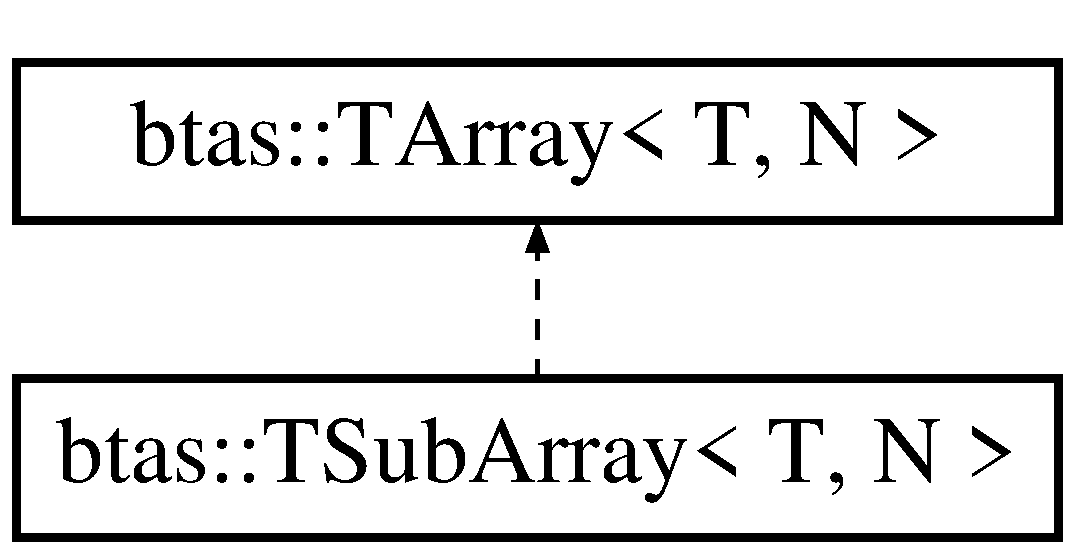
\includegraphics[height=2.000000cm]{da/d50/classbtas_1_1TSubArray}
\end{center}
\end{figure}
\subsection*{Public Member Functions}
\begin{DoxyCompactItemize}
\item 
{\bf T\-Sub\-Array} (const {\bf T\-Array}$<$ T, N $>$ \&a, const {\bf I\-Vector}$<$ N $>$ \&lbound, const {\bf I\-Vector}$<$ N $>$ \&ubound)
\begin{DoxyCompactList}\small\item\em Constructor, from dense array object and lower/upper boundary indices. \end{DoxyCompactList}\item 
{\footnotesize template$<$size\-\_\-t M$>$ }\\void {\bf copy} (const {\bf T\-Array}$<$ T, M $>$ \&a)
\begin{DoxyCompactList}\small\item\em Copy from array to sub-\/array. \end{DoxyCompactList}\item 
{\footnotesize template$<$size\-\_\-t M$>$ }\\void {\bf operator=} (const {\bf T\-Array}$<$ T, M $>$ \&other)
\begin{DoxyCompactList}\small\item\em Copy assignment operator from \doxyref{T\-Array}{p.}{db/d3c/classbtas_1_1TArray}. \end{DoxyCompactList}\end{DoxyCompactItemize}
\subsection*{Private Member Functions}
\begin{DoxyCompactItemize}
\item 
{\bf T\-Sub\-Array} ()
\begin{DoxyCompactList}\small\item\em Not default-\/constructible. \end{DoxyCompactList}\end{DoxyCompactItemize}
\subsection*{Private Attributes}
\begin{DoxyCompactItemize}
\item 
{\bf I\-Vector}$<$ N $>$ {\bf m\-\_\-lower\-\_\-bound}
\begin{DoxyCompactList}\small\item\em lower boundary indices \end{DoxyCompactList}\item 
{\bf I\-Vector}$<$ N $>$ {\bf m\-\_\-upper\-\_\-bound}
\begin{DoxyCompactList}\small\item\em upper boundary indices \end{DoxyCompactList}\end{DoxyCompactItemize}
\subsection*{Friends}
\begin{DoxyCompactItemize}
\item 
{\footnotesize template$<$typename U , size\-\_\-t M$>$ }\\class {\bf T\-Array}
\begin{DoxyCompactList}\small\item\em Any \doxyref{T\-Array}{p.}{db/d3c/classbtas_1_1TArray} classes being friend of T\-Sub\-Array$<$\-T, N$>$ \end{DoxyCompactList}\end{DoxyCompactItemize}
\subsection*{Additional Inherited Members}


\subsection{Detailed Description}
\subsubsection*{template$<$typename T, size\-\_\-t N$>$class btas\-::\-T\-Sub\-Array$<$ T, N $>$}

Sub-\/array of dense array \doxyref{T\-Array}{p.}{db/d3c/classbtas_1_1TArray}. 

Expression template providing copy semantics between \doxyref{T\-Array}{p.}{db/d3c/classbtas_1_1TArray} and \doxyref{T\-Sub\-Array}{p.}{da/d50/classbtas_1_1TSubArray} 
\begin{DoxyParams}{Parameters}
{\em T} & value type \\
\hline
{\em N} & array rank \\
\hline
\end{DoxyParams}


Definition at line 23 of file T\-Array.\-h.



\subsection{Constructor \& Destructor Documentation}
\index{btas\-::\-T\-Sub\-Array@{btas\-::\-T\-Sub\-Array}!T\-Sub\-Array@{T\-Sub\-Array}}
\index{T\-Sub\-Array@{T\-Sub\-Array}!btas::TSubArray@{btas\-::\-T\-Sub\-Array}}
\subsubsection[{T\-Sub\-Array}]{\setlength{\rightskip}{0pt plus 5cm}template$<$typename T, size\-\_\-t N$>$ {\bf btas\-::\-T\-Sub\-Array}$<$ T, N $>$\-::{\bf T\-Sub\-Array} (
\begin{DoxyParamCaption}
{}
\end{DoxyParamCaption}
)\hspace{0.3cm}{\ttfamily [private]}}\label{da/d50/classbtas_1_1TSubArray_a09b7333f2c1e5a8bf64682c2d586ad0d}


Not default-\/constructible. 

\index{btas\-::\-T\-Sub\-Array@{btas\-::\-T\-Sub\-Array}!T\-Sub\-Array@{T\-Sub\-Array}}
\index{T\-Sub\-Array@{T\-Sub\-Array}!btas::TSubArray@{btas\-::\-T\-Sub\-Array}}
\subsubsection[{T\-Sub\-Array}]{\setlength{\rightskip}{0pt plus 5cm}template$<$typename T, size\-\_\-t N$>$ {\bf btas\-::\-T\-Sub\-Array}$<$ T, N $>$\-::{\bf T\-Sub\-Array} (
\begin{DoxyParamCaption}
\item[{const {\bf T\-Array}$<$ T, N $>$ \&}]{a, }
\item[{const {\bf I\-Vector}$<$ N $>$ \&}]{lbound, }
\item[{const {\bf I\-Vector}$<$ N $>$ \&}]{ubound}
\end{DoxyParamCaption}
)\hspace{0.3cm}{\ttfamily [inline]}}\label{da/d50/classbtas_1_1TSubArray_aa11f07f95ff0bc35712dedb9c91c1b01}


Constructor, from dense array object and lower/upper boundary indices. 



Definition at line 39 of file T\-Sub\-Array.\-h.



References btas\-::\-T\-Sub\-Array$<$ T, N $>$\-::m\-\_\-lower\-\_\-bound, btas\-::\-T\-Sub\-Array$<$ T, N $>$\-::m\-\_\-upper\-\_\-bound, and btas\-::\-T\-Array$<$ T, N $>$\-::reference().



\subsection{Member Function Documentation}
\index{btas\-::\-T\-Sub\-Array@{btas\-::\-T\-Sub\-Array}!copy@{copy}}
\index{copy@{copy}!btas::TSubArray@{btas\-::\-T\-Sub\-Array}}
\subsubsection[{copy}]{\setlength{\rightskip}{0pt plus 5cm}template$<$typename T, size\-\_\-t N$>$ template$<$size\-\_\-t M$>$ void {\bf btas\-::\-T\-Sub\-Array}$<$ T, N $>$\-::copy (
\begin{DoxyParamCaption}
\item[{const {\bf T\-Array}$<$ T, M $>$ \&}]{a}
\end{DoxyParamCaption}
)\hspace{0.3cm}{\ttfamily [inline]}}\label{da/d50/classbtas_1_1TSubArray_a27a85be70497eafeeaa2a2a8b8b0a0e4}


Copy from array to sub-\/array. 



Definition at line 47 of file T\-Sub\-Array.\-h.



References btas\-::\-\_\-fast\-\_\-copy(), btas\-::\-T\-Array$<$ T, N $>$\-::data(), btas\-::dot(), btas\-::\-T\-Sub\-Array$<$ T, N $>$\-::m\-\_\-lower\-\_\-bound, btas\-::\-T\-Array$<$ T, N $>$\-::m\-\_\-stride, btas\-::\-T\-Sub\-Array$<$ T, N $>$\-::m\-\_\-upper\-\_\-bound, and btas\-::\-T\-Array$<$ T, N $>$\-::size().

\index{btas\-::\-T\-Sub\-Array@{btas\-::\-T\-Sub\-Array}!operator=@{operator=}}
\index{operator=@{operator=}!btas::TSubArray@{btas\-::\-T\-Sub\-Array}}
\subsubsection[{operator=}]{\setlength{\rightskip}{0pt plus 5cm}template$<$typename T, size\-\_\-t N$>$ template$<$size\-\_\-t M$>$ void {\bf btas\-::\-T\-Sub\-Array}$<$ T, N $>$\-::operator= (
\begin{DoxyParamCaption}
\item[{const {\bf T\-Array}$<$ T, M $>$ \&}]{other}
\end{DoxyParamCaption}
)\hspace{0.3cm}{\ttfamily [inline]}}\label{da/d50/classbtas_1_1TSubArray_aee4f1e815c2c83a03a20cd01d6e95259}


Copy assignment operator from \doxyref{T\-Array}{p.}{db/d3c/classbtas_1_1TArray}. 



Definition at line 76 of file T\-Sub\-Array.\-h.



References btas\-::\-T\-Array$<$ T, N $>$\-::copy().



\subsection{Friends And Related Function Documentation}
\index{btas\-::\-T\-Sub\-Array@{btas\-::\-T\-Sub\-Array}!T\-Array@{T\-Array}}
\index{T\-Array@{T\-Array}!btas::TSubArray@{btas\-::\-T\-Sub\-Array}}
\subsubsection[{T\-Array}]{\setlength{\rightskip}{0pt plus 5cm}template$<$typename T, size\-\_\-t N$>$ template$<$typename U , size\-\_\-t M$>$ friend class {\bf T\-Array}\hspace{0.3cm}{\ttfamily [friend]}}\label{da/d50/classbtas_1_1TSubArray_aa262c41fb2786ee01ea853b18e55a362}


Any \doxyref{T\-Array}{p.}{db/d3c/classbtas_1_1TArray} classes being friend of T\-Sub\-Array$<$\-T, N$>$ 



Definition at line 31 of file T\-Sub\-Array.\-h.



\subsection{Field Documentation}
\index{btas\-::\-T\-Sub\-Array@{btas\-::\-T\-Sub\-Array}!m\-\_\-lower\-\_\-bound@{m\-\_\-lower\-\_\-bound}}
\index{m\-\_\-lower\-\_\-bound@{m\-\_\-lower\-\_\-bound}!btas::TSubArray@{btas\-::\-T\-Sub\-Array}}
\subsubsection[{m\-\_\-lower\-\_\-bound}]{\setlength{\rightskip}{0pt plus 5cm}template$<$typename T, size\-\_\-t N$>$ {\bf I\-Vector}$<$N$>$ {\bf btas\-::\-T\-Sub\-Array}$<$ T, N $>$\-::m\-\_\-lower\-\_\-bound\hspace{0.3cm}{\ttfamily [private]}}\label{da/d50/classbtas_1_1TSubArray_a24984c0181c10b48a7dc7e8b1d05a6f6}


lower boundary indices 



Definition at line 81 of file T\-Sub\-Array.\-h.



Referenced by btas\-::\-T\-Sub\-Array$<$ T, N $>$\-::copy(), btas\-::\-T\-Array$<$ T, N $>$\-::copy(), and btas\-::\-T\-Sub\-Array$<$ T, N $>$\-::\-T\-Sub\-Array().

\index{btas\-::\-T\-Sub\-Array@{btas\-::\-T\-Sub\-Array}!m\-\_\-upper\-\_\-bound@{m\-\_\-upper\-\_\-bound}}
\index{m\-\_\-upper\-\_\-bound@{m\-\_\-upper\-\_\-bound}!btas::TSubArray@{btas\-::\-T\-Sub\-Array}}
\subsubsection[{m\-\_\-upper\-\_\-bound}]{\setlength{\rightskip}{0pt plus 5cm}template$<$typename T, size\-\_\-t N$>$ {\bf I\-Vector}$<$N$>$ {\bf btas\-::\-T\-Sub\-Array}$<$ T, N $>$\-::m\-\_\-upper\-\_\-bound\hspace{0.3cm}{\ttfamily [private]}}\label{da/d50/classbtas_1_1TSubArray_ab74af8bc5586e84d8a95b1779668900e}


upper boundary indices 



Definition at line 84 of file T\-Sub\-Array.\-h.



Referenced by btas\-::\-T\-Sub\-Array$<$ T, N $>$\-::copy(), btas\-::\-T\-Array$<$ T, N $>$\-::copy(), and btas\-::\-T\-Sub\-Array$<$ T, N $>$\-::\-T\-Sub\-Array().



The documentation for this class was generated from the following files\-:\begin{DoxyCompactItemize}
\item 
include/btas/\-D\-E\-N\-S\-E/{\bf T\-Array.\-h}\item 
include/btas/\-D\-E\-N\-S\-E/{\bf T\-Sub\-Array.\-h}\end{DoxyCompactItemize}

\chapter{File Documentation}
\section{include/btas/blas\-\_\-cxx\-\_\-interface.h File Reference}
\label{dd/d03/blas__cxx__interface_8h}\index{include/btas/blas\-\_\-cxx\-\_\-interface.\-h@{include/btas/blas\-\_\-cxx\-\_\-interface.\-h}}
\subsection*{Namespaces}
\begin{DoxyCompactItemize}
\item 
namespace {\bf btas}
\end{DoxyCompactItemize}
\subsection*{Enumerations}
\begin{DoxyCompactItemize}
\item 
enum {\bf btas\-::\-B\-T\-A\-S\-\_\-\-O\-R\-D\-E\-R} \{ {\bf btas\-::\-Row\-Major} =101, 
{\bf btas\-::\-Col\-Major} =102
 \}
\item 
enum {\bf btas\-::\-B\-T\-A\-S\-\_\-\-T\-R\-A\-N\-S\-P\-O\-S\-E} \{ {\bf btas\-::\-No\-Trans} =111, 
{\bf btas\-::\-Trans} =112, 
{\bf btas\-::\-Conj\-Trans} =113
 \}
\item 
enum {\bf btas\-::\-B\-T\-A\-S\-\_\-\-U\-P\-L\-O} \{ {\bf btas\-::\-Upper} =121, 
{\bf btas\-::\-Lower} =122
 \}
\item 
enum {\bf btas\-::\-B\-T\-A\-S\-\_\-\-D\-I\-A\-G} \{ {\bf btas\-::\-Non\-Unit} =131, 
{\bf btas\-::\-Unit} =132
 \}
\item 
enum {\bf btas\-::\-B\-T\-A\-S\-\_\-\-S\-I\-D\-E} \{ {\bf btas\-::\-Left} =141, 
{\bf btas\-::\-Right} =142
 \}
\end{DoxyCompactItemize}

\section{include/btas/btas.h File Reference}
\label{d9/d0b/btas_8h}\index{include/btas/btas.\-h@{include/btas/btas.\-h}}
{\ttfamily \#include $<$vector$>$}\\*
{\ttfamily \#include $<$cassert$>$}\\*
{\ttfamily \#include $<$boost/function.\-hpp$>$}\\*
{\ttfamily \#include $<$boost/bind.\-hpp$>$}\\*
{\ttfamily \#include $<$boost/shared\-\_\-ptr.\-hpp$>$}\\*
{\ttfamily \#include $<$iostream$>$}\\*
{\ttfamily \#include $<$stdexcept$>$}\\*
\subsection*{Data Structures}
\begin{DoxyCompactItemize}
\item 
struct {\bf btas\-::null\-\_\-deleter}
\begin{DoxyCompactList}\small\item\em Null-\/deleter. \end{DoxyCompactList}\end{DoxyCompactItemize}
\subsection*{Namespaces}
\begin{DoxyCompactItemize}
\item 
namespace {\bf btas}
\end{DoxyCompactItemize}
\subsection*{Macros}
\begin{DoxyCompactItemize}
\item 
\#define {\bf B\-T\-A\-S\-\_\-\-D\-E\-B\-U\-G}(msg)~\{ std\-::cout $<$$<$ \char`\"{}B\-T\-A\-S\-\_\-\-D\-E\-B\-U\-G\-: \char`\"{} $<$$<$ msg $<$$<$ std\-::endl; \}
\item 
\#define {\bf B\-T\-A\-S\-\_\-\-T\-H\-R\-O\-W}(truth, msg)~\{ if (!(truth)) \{ throw std\-::runtime\-\_\-error(msg); \} \}
\end{DoxyCompactItemize}
\subsection*{Typedefs}
\begin{DoxyCompactItemize}
\item 
typedef unsigned int {\bf btas\-::uint}
\item 
typedef unsigned long {\bf btas\-::wint}
\item 
typedef std\-::vector$<$ int $>$ {\bf btas\-::\-Dshapes}
\begin{DoxyCompactList}\small\item\em Alias to dense shape. \end{DoxyCompactList}\end{DoxyCompactItemize}


\subsection{Macro Definition Documentation}
\index{btas.\-h@{btas.\-h}!B\-T\-A\-S\-\_\-\-D\-E\-B\-U\-G@{B\-T\-A\-S\-\_\-\-D\-E\-B\-U\-G}}
\index{B\-T\-A\-S\-\_\-\-D\-E\-B\-U\-G@{B\-T\-A\-S\-\_\-\-D\-E\-B\-U\-G}!btas.h@{btas.\-h}}
\subsubsection[{B\-T\-A\-S\-\_\-\-D\-E\-B\-U\-G}]{\setlength{\rightskip}{0pt plus 5cm}\#define B\-T\-A\-S\-\_\-\-D\-E\-B\-U\-G(
\begin{DoxyParamCaption}
\item[{}]{msg}
\end{DoxyParamCaption}
)~\{ std\-::cout $<$$<$ \char`\"{}B\-T\-A\-S\-\_\-\-D\-E\-B\-U\-G\-: \char`\"{} $<$$<$ msg $<$$<$ std\-::endl; \}}\label{d9/d0b/btas_8h_ac73961bcc680d1ef31b40e4ebfdf7934}


Definition at line 15 of file btas.\-h.



Referenced by btas\-::\-S\-T\-Array$<$ T, N $>$\-::insert(), and btas\-::\-S\-T\-Array$<$ T, N $>$\-::reserve().

\index{btas.\-h@{btas.\-h}!B\-T\-A\-S\-\_\-\-T\-H\-R\-O\-W@{B\-T\-A\-S\-\_\-\-T\-H\-R\-O\-W}}
\index{B\-T\-A\-S\-\_\-\-T\-H\-R\-O\-W@{B\-T\-A\-S\-\_\-\-T\-H\-R\-O\-W}!btas.h@{btas.\-h}}
\subsubsection[{B\-T\-A\-S\-\_\-\-T\-H\-R\-O\-W}]{\setlength{\rightskip}{0pt plus 5cm}\#define B\-T\-A\-S\-\_\-\-T\-H\-R\-O\-W(
\begin{DoxyParamCaption}
\item[{}]{truth, }
\item[{}]{msg}
\end{DoxyParamCaption}
)~\{ if (!(truth)) \{ throw std\-::runtime\-\_\-error(msg); \} \}}\label{d9/d0b/btas_8h_a72a16136c71a8dcec00647cb8aff51e2}


Definition at line 19 of file btas.\-h.



Referenced by mps\-::add(), btas\-::\-S\-T\-Array$<$ T, N $>$\-::check\-\_\-net\-\_\-dshape(), btas\-::\-Daxpy(), btas\-::\-Dcontract(), btas\-::\-Dcopy\-Flatten(), btas\-::\-Ddiagonal(), btas\-::\-Ddidm(), btas\-::\-Ddimd(), btas\-::\-Ddot(), btas\-::decompose\-\_\-shape(), btas\-::\-Dgeev(), btas\-::\-Dgemm(), btas\-::\-Dgemv(), btas\-::\-Dger(), btas\-::\-Dgesv(), btas\-::\-Dgesvd(), btas\-::\-Dgetrf(), btas\-::\-Dggev(), btas\-::\-Dpermute(), btas\-::\-Dreindex(), btas\-::\-Dsyev(), btas\-::\-Dsygv(), mps\-::gemm(), btas\-::gemm\-\_\-contract\-\_\-dshape(), btas\-::gemm\-\_\-contract\-\_\-qshape(), btas\-::gemm\-\_\-contract\-\_\-shape(), mps\-::gemv(), btas\-::gemv\-\_\-contract\-\_\-dshape(), btas\-::gemv\-\_\-contract\-\_\-qshape(), btas\-::gemv\-\_\-contract\-\_\-shape(), btas\-::ger\-\_\-contract\-\_\-shape(), btas\-::indexed\-\_\-contract\-\_\-shape(), btas\-::indexed\-\_\-decompose\-\_\-shape(), btas\-::indexed\-\_\-permute\-\_\-shape(), mps\-::inprod(), btas\-::\-S\-T\-Array$<$ T, N $>$\-::mf\-\_\-check\-\_\-dshape(), btas\-::\-Q\-S\-Daxpy(), btas\-::\-Q\-S\-Dcontract(), btas\-::\-Q\-S\-Ddotc(), btas\-::\-Q\-S\-Ddotu(), btas\-::\-Q\-S\-Dgemm(), btas\-::\-Q\-S\-Dgemv(), btas\-::\-Q\-S\-Dger(), btas\-::\-Q\-S\-Dpermute(), btas\-::\-Q\-S\-Tdsum(), btas\-::\-S\-T\-Array$<$ T, N $>$\-::reserve(), btas\-::\-Q\-S\-Tmerge\-Info$<$ N, Q $>$\-::reset(), btas\-::\-S\-Daxpy(), btas\-::\-S\-Dcontract(), btas\-::\-S\-Dcopy(), btas\-::\-S\-Ddiagonal(), btas\-::\-S\-Ddot(), btas\-::\-S\-Dgemm(), btas\-::\-S\-Dgemv(), btas\-::\-S\-Dger(), btas\-::\-S\-Dpermute(), btas\-::serial\-\_\-\-S\-Daxpy(), btas\-::serial\-\_\-\-S\-Dcopy(), btas\-::\-S\-Tdsum(), btas\-::thread\-\_\-\-S\-Daxpy(), btas\-::thread\-\_\-\-S\-Dcopy(), btas\-::thread\-\_\-\-S\-Dgemm(), btas\-::thread\-\_\-\-S\-Dgemv(), and btas\-::thread\-\_\-\-S\-Dger().


\section{include/btas/btas\-\_\-contract\-\_\-shape.h File Reference}
\label{dd/d9e/btas__contract__shape_8h}\index{include/btas/btas\-\_\-contract\-\_\-shape.\-h@{include/btas/btas\-\_\-contract\-\_\-shape.\-h}}
{\ttfamily \#include $<$vector$>$}\\*
{\ttfamily \#include $<$set$>$}\\*
{\ttfamily \#include $<$map$>$}\\*
{\ttfamily \#include $<$algorithm$>$}\\*
{\ttfamily \#include $<$btas/btas.\-h$>$}\\*
{\ttfamily \#include $<$btas/\-T\-Vector.\-h$>$}\\*
{\ttfamily \#include $<$btas/blas\-\_\-cxx\-\_\-interface.\-h$>$}\\*
\subsection*{Namespaces}
\begin{DoxyCompactItemize}
\item 
namespace {\bf btas}
\end{DoxyCompactItemize}
\subsection*{Enumerations}
\begin{DoxyCompactItemize}
\item 
enum {\bf btas\-::\-B\-T\-A\-S\-\_\-\-C\-O\-N\-T\-R\-A\-C\-T\-\_\-\-T\-U\-N\-I\-N\-G} \{ \\*
{\bf btas\-::\-J\-O\-B\-M\-A\-S\-K\-\_\-\-A\-\_\-\-P\-M\-U\-T\-E} = 0x20, 
{\bf btas\-::\-J\-O\-B\-M\-A\-S\-K\-\_\-\-A\-\_\-\-T\-R\-A\-N\-S} = 0x10, 
{\bf btas\-::\-J\-O\-B\-M\-A\-S\-K\-\_\-\-B\-\_\-\-P\-M\-U\-T\-E} = 0x08, 
{\bf btas\-::\-J\-O\-B\-M\-A\-S\-K\-\_\-\-B\-\_\-\-T\-R\-A\-N\-S} = 0x04, 
\\*
{\bf btas\-::\-J\-O\-B\-M\-A\-S\-K\-\_\-\-B\-L\-A\-S\-\_\-\-T\-Y\-P\-E} = 0x03
 \}
\end{DoxyCompactItemize}
\subsection*{Functions}
\begin{DoxyCompactItemize}
\item 
{\footnotesize template$<$size\-\_\-t N\-A, size\-\_\-t N\-B, size\-\_\-t N\-C$>$ }\\void {\bf btas\-::gemv\-\_\-contract\-\_\-shape} (const B\-T\-A\-S\-\_\-\-T\-R\-A\-N\-S\-P\-O\-S\-E \&Trans\-A, const I\-Vector$<$ N\-A $>$ \&a\-\_\-shape, const I\-Vector$<$ N\-B $>$ \&b\-\_\-shape, I\-Vector$<$ N\-C $>$ \&c\-\_\-shape)
\item 
{\footnotesize template$<$size\-\_\-t N\-A, size\-\_\-t N\-B, size\-\_\-t N\-C$>$ }\\void {\bf btas\-::ger\-\_\-contract\-\_\-shape} (const I\-Vector$<$ N\-A $>$ \&a\-\_\-shape, const I\-Vector$<$ N\-B $>$ \&b\-\_\-shape, I\-Vector$<$ N\-C $>$ \&c\-\_\-shape)
\item 
{\footnotesize template$<$size\-\_\-t N\-A, size\-\_\-t N\-B, size\-\_\-t N\-C, size\-\_\-t K$>$ }\\void {\bf btas\-::gemm\-\_\-contract\-\_\-shape} (const B\-T\-A\-S\-\_\-\-T\-R\-A\-N\-S\-P\-O\-S\-E \&Trans\-A, const B\-T\-A\-S\-\_\-\-T\-R\-A\-N\-S\-P\-O\-S\-E \&Trans\-B, const I\-Vector$<$ N\-A $>$ \&a\-\_\-shape, const I\-Vector$<$ N\-B $>$ \&b\-\_\-shape, I\-Vector$<$ K $>$ \&contracts, I\-Vector$<$ N\-C $>$ \&c\-\_\-shape)
\item 
{\footnotesize template$<$size\-\_\-t N\-A, size\-\_\-t N\-B, size\-\_\-t K$>$ }\\unsigned int {\bf btas\-::get\-\_\-contract\-\_\-jobs} (const I\-Vector$<$ N\-A $>$ \&a\-\_\-shape, const I\-Vector$<$ K $>$ \&a\-\_\-contract, I\-Vector$<$ N\-A $>$ \&a\-\_\-permute, const I\-Vector$<$ N\-B $>$ \&b\-\_\-shape, const I\-Vector$<$ K $>$ \&b\-\_\-contract, I\-Vector$<$ N\-B $>$ \&b\-\_\-permute)
\item 
{\footnotesize template$<$size\-\_\-t N\-A, size\-\_\-t N\-B, size\-\_\-t K$>$ }\\void {\bf btas\-::indexed\-\_\-contract\-\_\-shape} (const I\-Vector$<$ N\-A $>$ \&a\-\_\-symbols, I\-Vector$<$ K $>$ \&a\-\_\-contract, const I\-Vector$<$ N\-B $>$ \&b\-\_\-symbols, I\-Vector$<$ K $>$ \&b\-\_\-contract, I\-Vector$<$ N\-A+N\-B-\/K-\/K $>$ \&axb\-\_\-symbols)
\end{DoxyCompactItemize}

\section{include/btas/btas\-\_\-permute\-\_\-shape.h File Reference}
\label{dc/d2e/btas__permute__shape_8h}\index{include/btas/btas\-\_\-permute\-\_\-shape.\-h@{include/btas/btas\-\_\-permute\-\_\-shape.\-h}}
{\ttfamily \#include $<$set$>$}\\*
{\ttfamily \#include $<$map$>$}\\*
{\ttfamily \#include $<$btas/btas.\-h$>$}\\*
{\ttfamily \#include $<$btas/\-T\-Vector.\-h$>$}\\*
\subsection*{Namespaces}
\begin{DoxyCompactItemize}
\item 
namespace {\bf btas}
\end{DoxyCompactItemize}
\subsection*{Functions}
\begin{DoxyCompactItemize}
\item 
{\footnotesize template$<$size\-\_\-t N$>$ }\\void {\bf btas\-::permute\-\_\-shape} (const I\-Vector$<$ N $>$ \&pindex, const I\-Vector$<$ N $>$ \&xshape, I\-Vector$<$ N $>$ \&xstrides, I\-Vector$<$ N $>$ \&yshape)
\item 
{\footnotesize template$<$size\-\_\-t N$>$ }\\void {\bf btas\-::indexed\-\_\-permute\-\_\-shape} (const I\-Vector$<$ N $>$ \&x\-\_\-symbols, const I\-Vector$<$ N $>$ \&y\-\_\-symbols, I\-Vector$<$ N $>$ \&pindex)
\end{DoxyCompactItemize}

\section{include/btas/\-D\-E\-N\-S\-E/\-C\-Array.h File Reference}
\label{d9/d78/CArray_8h}\index{include/btas/\-D\-E\-N\-S\-E/\-C\-Array.\-h@{include/btas/\-D\-E\-N\-S\-E/\-C\-Array.\-h}}


Dense array for single precision complex number.  


{\ttfamily \#include $<$iostream$>$}\\*
{\ttfamily \#include $<$iomanip$>$}\\*
{\ttfamily \#include $<$cmath$>$}\\*
{\ttfamily \#include $<$btas/\-T\-Vector.\-h$>$}\\*
{\ttfamily \#include $<$btas/blas\-\_\-cxx\-\_\-interface.\-h$>$}\\*
{\ttfamily \#include $<$btas/\-D\-E\-N\-S\-E/\-T\-Array.\-h$>$}\\*
{\ttfamily \#include $<$btas/\-D\-E\-N\-S\-E/\-T\-Sub\-Array.\-h$>$}\\*
\subsection*{Namespaces}
\begin{DoxyCompactItemize}
\item 
namespace {\bf btas}
\end{DoxyCompactItemize}
\subsection*{Typedefs}
\begin{DoxyCompactItemize}
\item 
{\footnotesize template$<$size\-\_\-t N$>$ }\\using {\bf btas\-::\-C\-Array} = T\-Array$<$ complex$<$ float $>$, N $>$
\begin{DoxyCompactList}\small\item\em Alias to single precision complex array. \end{DoxyCompactList}\item 
{\footnotesize template$<$size\-\_\-t N$>$ }\\using {\bf btas\-::\-C\-Sub\-Array} = T\-Sub\-Array$<$ complex$<$ float $>$, N $>$
\begin{DoxyCompactList}\small\item\em Alias to single precision complex sub-\/array. \end{DoxyCompactList}\end{DoxyCompactItemize}
\subsection*{Functions}
\begin{DoxyCompactItemize}
\item 
{\footnotesize template$<$$>$ }\\void {\bf btas\-::\-\_\-fast\-\_\-copy$<$ complex$<$ float $>$ $>$} (size\-\_\-t n, const complex$<$ float $>$ $\ast$x, complex$<$ float $>$ $\ast$y)
\begin{DoxyCompactList}\small\item\em Fast copying for single precision complex array (calling cblas\-\_\-ccopy) \end{DoxyCompactList}\item 
{\footnotesize template$<$$>$ }\\void {\bf btas\-::\-\_\-fast\-\_\-scal$<$ complex$<$ float $>$ $>$} (size\-\_\-t n, const complex$<$ float $>$ \&alpha, complex$<$ float $>$ $\ast$x)
\begin{DoxyCompactList}\small\item\em Fast scaling for single precision complex array (calling cblas\-\_\-cscal) \end{DoxyCompactList}\item 
{\footnotesize template$<$$>$ }\\void {\bf btas\-::\-\_\-fast\-\_\-add$<$ complex$<$ float $>$ $>$} (size\-\_\-t n, const complex$<$ float $>$ $\ast$x, complex$<$ float $>$ $\ast$y)
\begin{DoxyCompactList}\small\item\em Fast adding for single precision complex array (calling cblas\-\_\-caxpy) \end{DoxyCompactList}\item 
{\footnotesize template$<$size\-\_\-t N$>$ }\\std\-::ostream \& {\bf operator$<$$<$} (std\-::ostream \&ost, const {\bf btas\-::\-C\-Array}$<$ N $>$ \&a)
\begin{DoxyCompactList}\small\item\em C++ style printing function. \end{DoxyCompactList}\end{DoxyCompactItemize}


\subsection{Detailed Description}
Dense array for single precision complex number. 

Definition in file {\bf C\-Array.\-h}.



\subsection{Function Documentation}
\index{C\-Array.\-h@{C\-Array.\-h}!operator$<$$<$@{operator$<$$<$}}
\index{operator$<$$<$@{operator$<$$<$}!CArray.h@{C\-Array.\-h}}
\subsubsection[{operator$<$$<$}]{\setlength{\rightskip}{0pt plus 5cm}template$<$size\-\_\-t N$>$ std\-::ostream\& operator$<$$<$ (
\begin{DoxyParamCaption}
\item[{std\-::ostream \&}]{ost, }
\item[{const {\bf btas\-::\-C\-Array}$<$ N $>$ \&}]{a}
\end{DoxyParamCaption}
)}\label{d9/d78/CArray_8h_a1c64c122bd6269e064dbb394b4492c4e}


C++ style printing function. 



Definition at line 52 of file C\-Array.\-h.


\section{include/btas/\-D\-E\-N\-S\-E/\-Darglist.h File Reference}
\label{d4/d22/Darglist_8h}\index{include/btas/\-D\-E\-N\-S\-E/\-Darglist.\-h@{include/btas/\-D\-E\-N\-S\-E/\-Darglist.\-h}}
{\ttfamily \#include $<$functional$>$}\\*
{\ttfamily \#include $<$numeric$>$}\\*
{\ttfamily \#include $<$btas/\-Targlist.\-h$>$}\\*
{\ttfamily \#include $<$btas/\-D\-E\-N\-S\-E/\-Dblas.\-h$>$}\\*
{\ttfamily \#include $<$btas/\-D\-E\-N\-S\-E/\-Dpermute.\-h$>$}\\*
{\ttfamily \#include $<$btas/\-D\-E\-N\-S\-E/\-Dlapack.\-h$>$}\\*
\subsection*{Data Structures}
\begin{DoxyCompactItemize}
\item 
class {\bf btas\-::\-Dcopy\-Arglist$<$ N $>$}
\item 
class {\bf btas\-::\-Dscal\-Arglist$<$ N $>$}
\item 
class {\bf btas\-::\-Daxpy\-Arglist$<$ N $>$}
\item 
class {\bf btas\-::\-Dpermute\-Arglist$<$ N $>$}
\item 
class {\bf btas\-::\-Dgemv\-Arglist$<$ N\-A, N\-B, N\-C $>$}
\item 
class {\bf btas\-::\-Dger\-Arglist$<$ N\-A, N\-B, N\-C $>$}
\item 
class {\bf btas\-::\-Dgemm\-Arglist$<$ N\-A, N\-B, N\-C $>$}
\item 
class {\bf btas\-::\-Dgesvd\-Arglist$<$ N\-A, N\-U $>$}
\end{DoxyCompactItemize}
\subsection*{Namespaces}
\begin{DoxyCompactItemize}
\item 
namespace {\bf btas}
\end{DoxyCompactItemize}

\section{include/btas/\-D\-E\-N\-S\-E/\-D\-Array.h File Reference}
\label{d3/d5c/DArray_8h}\index{include/btas/\-D\-E\-N\-S\-E/\-D\-Array.\-h@{include/btas/\-D\-E\-N\-S\-E/\-D\-Array.\-h}}


Dense array for double precision real number.  


{\ttfamily \#include $<$iostream$>$}\\*
{\ttfamily \#include $<$iomanip$>$}\\*
{\ttfamily \#include $<$btas/\-T\-Vector.\-h$>$}\\*
{\ttfamily \#include $<$btas/blas\-\_\-cxx\-\_\-interface.\-h$>$}\\*
{\ttfamily \#include $<$btas/\-D\-E\-N\-S\-E/\-T\-Array.\-h$>$}\\*
{\ttfamily \#include $<$btas/\-D\-E\-N\-S\-E/\-T\-Sub\-Array.\-h$>$}\\*
{\ttfamily \#include $<$btas/\-D\-E\-N\-S\-E/\-Dblas.\-h$>$}\\*
{\ttfamily \#include $<$btas/\-D\-E\-N\-S\-E/\-Dlapack.\-h$>$}\\*
{\ttfamily \#include $<$btas/\-D\-E\-N\-S\-E/\-Dpermute.\-h$>$}\\*
{\ttfamily \#include $<$btas/\-D\-E\-N\-S\-E/\-Dcontract.\-h$>$}\\*
{\ttfamily \#include $<$btas/\-D\-E\-N\-S\-E/\-Ddiagonal.\-h$>$}\\*
\subsection*{Namespaces}
\begin{DoxyCompactItemize}
\item 
namespace {\bf btas}
\end{DoxyCompactItemize}
\subsection*{Typedefs}
\begin{DoxyCompactItemize}
\item 
{\footnotesize template$<$size\-\_\-t N$>$ }\\using {\bf btas\-::\-D\-Array} = T\-Array$<$ double, N $>$
\begin{DoxyCompactList}\small\item\em Alias to double precision real array. \end{DoxyCompactList}\item 
{\footnotesize template$<$size\-\_\-t N$>$ }\\using {\bf btas\-::\-D\-Sub\-Array} = T\-Sub\-Array$<$ double, N $>$
\begin{DoxyCompactList}\small\item\em Alias to double precision real sub-\/array. \end{DoxyCompactList}\end{DoxyCompactItemize}
\subsection*{Functions}
\begin{DoxyCompactItemize}
\item 
{\footnotesize template$<$$>$ }\\void {\bf btas\-::\-\_\-fast\-\_\-copy$<$ double $>$} (size\-\_\-t n, const double $\ast$x, double $\ast$y)
\begin{DoxyCompactList}\small\item\em Fast copying for double precision real array (calling cblas\-\_\-dcopy) \end{DoxyCompactList}\item 
{\footnotesize template$<$$>$ }\\void {\bf btas\-::\-\_\-fast\-\_\-scal$<$ double $>$} (size\-\_\-t n, const double \&alpha, double $\ast$x)
\begin{DoxyCompactList}\small\item\em Fast scaling for double precision real array (calling cblas\-\_\-dscal) \end{DoxyCompactList}\item 
{\footnotesize template$<$$>$ }\\void {\bf btas\-::\-\_\-fast\-\_\-add$<$ double $>$} (size\-\_\-t n, const double $\ast$x, double $\ast$y)
\begin{DoxyCompactList}\small\item\em Fast adding for double precision real array (calling cblas\-\_\-daxpy) \end{DoxyCompactList}\item 
{\footnotesize template$<$size\-\_\-t N$>$ }\\std\-::ostream \& {\bf operator$<$$<$} (std\-::ostream \&ost, const {\bf btas\-::\-D\-Array}$<$ N $>$ \&a)
\begin{DoxyCompactList}\small\item\em C++ style printing function. \end{DoxyCompactList}\end{DoxyCompactItemize}


\subsection{Detailed Description}
Dense array for double precision real number. 

Definition in file {\bf D\-Array.\-h}.



\subsection{Function Documentation}
\index{D\-Array.\-h@{D\-Array.\-h}!operator$<$$<$@{operator$<$$<$}}
\index{operator$<$$<$@{operator$<$$<$}!DArray.h@{D\-Array.\-h}}
\subsubsection[{operator$<$$<$}]{\setlength{\rightskip}{0pt plus 5cm}template$<$size\-\_\-t N$>$ std\-::ostream\& operator$<$$<$ (
\begin{DoxyParamCaption}
\item[{std\-::ostream \&}]{ost, }
\item[{const {\bf btas\-::\-D\-Array}$<$ N $>$ \&}]{a}
\end{DoxyParamCaption}
)}\label{d3/d5c/DArray_8h_a33560b01e12784586da1e3b8e4433fd2}


C++ style printing function. 



Definition at line 44 of file D\-Array.\-h.


\section{include/btas/\-D\-E\-N\-S\-E/\-Dblas.h File Reference}
\label{de/d3a/Dblas_8h}\index{include/btas/\-D\-E\-N\-S\-E/\-Dblas.\-h@{include/btas/\-D\-E\-N\-S\-E/\-Dblas.\-h}}


B\-L\-A\-S wrappers for double precision real array.  


{\ttfamily \#include $<$algorithm$>$}\\*
{\ttfamily \#include $<$numeric$>$}\\*
{\ttfamily \#include $<$btas/btas.\-h$>$}\\*
{\ttfamily \#include $<$btas/btas\-\_\-contract\-\_\-shape.\-h$>$}\\*
{\ttfamily \#include $<$btas/blas\-\_\-cxx\-\_\-interface.\-h$>$}\\*
{\ttfamily \#include $<$btas/\-D\-E\-N\-S\-E/\-D\-Array.\-h$>$}\\*
\subsection*{Namespaces}
\begin{DoxyCompactItemize}
\item 
namespace {\bf btas}
\end{DoxyCompactItemize}
\subsection*{Functions}
\begin{DoxyCompactItemize}
\item 
{\footnotesize template$<$size\-\_\-t N$>$ }\\void {\bf btas\-::\-Dcopy} (const D\-Array$<$ N $>$ \&x, D\-Array$<$ N $>$ \&y)
\begin{DoxyCompactList}\small\item\em D\-C\-O\-P\-Y\-: y \-:= x. \end{DoxyCompactList}\item 
{\footnotesize template$<$size\-\_\-t N\-X, size\-\_\-t N\-Y$>$ }\\void {\bf btas\-::\-Dcopy\-Flatten} (const D\-Array$<$ N\-X $>$ \&x, D\-Array$<$ N\-Y $>$ \&y)
\begin{DoxyCompactList}\small\item\em D\-C\-O\-P\-Y as flattened vectors\-: y \-:= x. \end{DoxyCompactList}\item 
{\footnotesize template$<$size\-\_\-t N\-X, size\-\_\-t N\-Y$>$ }\\void {\bf btas\-::\-Dreshape} (const D\-Array$<$ N\-X $>$ \&x, const I\-Vector$<$ N\-Y $>$ \&y\-\_\-shape, D\-Array$<$ N\-Y $>$ \&y)
\begin{DoxyCompactList}\small\item\em reshape rank of array \end{DoxyCompactList}\item 
{\footnotesize template$<$size\-\_\-t N$>$ }\\void {\bf btas\-::\-Dscal} (const double \&alpha, D\-Array$<$ N $>$ \&x)
\begin{DoxyCompactList}\small\item\em D\-S\-C\-A\-L\-: x \-:= alpha $\ast$ x. \end{DoxyCompactList}\item 
{\footnotesize template$<$size\-\_\-t N$>$ }\\void {\bf btas\-::\-Daxpy} (const double \&alpha, const D\-Array$<$ N $>$ \&x, D\-Array$<$ N $>$ \&y)
\begin{DoxyCompactList}\small\item\em D\-A\-X\-P\-Y\-: y \-:= alpha $\ast$ x + y. \end{DoxyCompactList}\item 
{\footnotesize template$<$size\-\_\-t N$>$ }\\double {\bf btas\-::\-Ddot} (const D\-Array$<$ N $>$ \&x, const D\-Array$<$ N $>$ \&y)
\begin{DoxyCompactList}\small\item\em D\-D\-O\-T\-: inner product of x and y. \end{DoxyCompactList}\item 
{\footnotesize template$<$size\-\_\-t N$>$ }\\double {\bf btas\-::\-Dnrm2} (const D\-Array$<$ N $>$ \&x)
\begin{DoxyCompactList}\small\item\em D\-N\-R\-M2\-: returns euclidean norm of x. \end{DoxyCompactList}\item 
{\footnotesize template$<$size\-\_\-t N\-A, size\-\_\-t N\-B, size\-\_\-t N\-C$>$ }\\void {\bf btas\-::\-Dgemv} (const B\-T\-A\-S\-\_\-\-T\-R\-A\-N\-S\-P\-O\-S\-E \&Trans\-A, const double \&alpha, const D\-Array$<$ N\-A $>$ \&a, const D\-Array$<$ N\-B $>$ \&b, const double \&beta, D\-Array$<$ N\-C $>$ \&c)
\begin{DoxyCompactList}\small\item\em D\-G\-E\-M\-V\-: Matrix-\/vector multiplication, c \-:= alphe $\ast$ a $\ast$ b + beta $\ast$ c. \end{DoxyCompactList}\item 
{\footnotesize template$<$size\-\_\-t N\-A, size\-\_\-t N\-B, size\-\_\-t N\-C$>$ }\\void {\bf btas\-::\-Dger} (const double \&alpha, const D\-Array$<$ N\-A $>$ \&a, const D\-Array$<$ N\-B $>$ \&b, D\-Array$<$ N\-C $>$ \&c)
\begin{DoxyCompactList}\small\item\em D\-G\-E\-R\-: Rank-\/update / direct product, c \-:= alpha $\ast$ ( a x b ) \end{DoxyCompactList}\item 
{\footnotesize template$<$size\-\_\-t N\-A, size\-\_\-t N\-B, size\-\_\-t N\-C$>$ }\\void {\bf btas\-::\-Dgemm} (const B\-T\-A\-S\-\_\-\-T\-R\-A\-N\-S\-P\-O\-S\-E \&Trans\-A, const B\-T\-A\-S\-\_\-\-T\-R\-A\-N\-S\-P\-O\-S\-E \&Trans\-B, const double \&alpha, const D\-Array$<$ N\-A $>$ \&a, const D\-Array$<$ N\-B $>$ \&b, const double \&beta, D\-Array$<$ N\-C $>$ \&c)
\begin{DoxyCompactList}\small\item\em D\-G\-E\-M\-M\-: Matrix-\/matrix multiplication, c \-:= alpha $\ast$ a $\ast$ b + beta $\ast$ c. \end{DoxyCompactList}\item 
{\footnotesize template$<$size\-\_\-t N\-A, size\-\_\-t N\-B$>$ }\\void {\bf btas\-::\-Ddimd} (D\-Array$<$ N\-A $>$ \&a, const D\-Array$<$ N\-B $>$ \&b)
\begin{DoxyCompactList}\small\item\em Non-\/\-B\-L\-A\-S function\-: a \-:= a(general matrix) $\ast$ b(diagonal matrix) \end{DoxyCompactList}\item 
{\footnotesize template$<$size\-\_\-t N\-A, size\-\_\-t N\-B$>$ }\\void {\bf btas\-::\-Ddidm} (const D\-Array$<$ N\-A $>$ \&a, D\-Array$<$ N\-B $>$ \&b)
\begin{DoxyCompactList}\small\item\em Non-\/\-B\-L\-A\-S function\-: b \-:= a(diagonal matrix) $\ast$ b(general matrix) \end{DoxyCompactList}\item 
{\footnotesize template$<$size\-\_\-t N\-A, size\-\_\-t N\-B, size\-\_\-t N\-C$>$ }\\void {\bf btas\-::\-Dblas\-Wrapper} (const double \&alpha, const D\-Array$<$ N\-A $>$ \&a, const D\-Array$<$ N\-B $>$ \&b, const double \&beta, D\-Array$<$ N\-C $>$ \&c)
\begin{DoxyCompactList}\small\item\em Wrapper function for D\-B\-L\-A\-S. \end{DoxyCompactList}\item 
{\footnotesize template$<$size\-\_\-t N$>$ }\\void {\bf btas\-::\-Dnormalize} (D\-Array$<$ N $>$ \&x)
\begin{DoxyCompactList}\small\item\em Normalization. \end{DoxyCompactList}\item 
{\footnotesize template$<$size\-\_\-t N$>$ }\\void {\bf btas\-::\-Dorthogonalize} (const D\-Array$<$ N $>$ \&x, D\-Array$<$ N $>$ \&y)
\begin{DoxyCompactList}\small\item\em Orthogonalization. \end{DoxyCompactList}\end{DoxyCompactItemize}


\subsection{Detailed Description}
B\-L\-A\-S wrappers for double precision real array. 

Definition in file {\bf Dblas.\-h}.


\section{include/btas/\-D\-E\-N\-S\-E/\-Dcontract.h File Reference}
\label{db/da1/Dcontract_8h}\index{include/btas/\-D\-E\-N\-S\-E/\-Dcontract.\-h@{include/btas/\-D\-E\-N\-S\-E/\-Dcontract.\-h}}
{\ttfamily \#include $<$btas/btas.\-h$>$}\\*
{\ttfamily \#include $<$btas/btas\-\_\-contract\-\_\-shape.\-h$>$}\\*
{\ttfamily \#include $<$btas/\-D\-E\-N\-S\-E/\-D\-Array.\-h$>$}\\*
{\ttfamily \#include $<$btas/\-D\-E\-N\-S\-E/\-Dblas.\-h$>$}\\*
{\ttfamily \#include $<$btas/\-D\-E\-N\-S\-E/\-Dpermute.\-h$>$}\\*
\subsection*{Namespaces}
\begin{DoxyCompactItemize}
\item 
namespace {\bf btas}
\end{DoxyCompactItemize}
\subsection*{Functions}
\begin{DoxyCompactItemize}
\item 
{\footnotesize template$<$size\-\_\-t N\-A, size\-\_\-t N\-B, size\-\_\-t K$>$ }\\void {\bf btas\-::\-Dcontract} (const double \&alpha, const D\-Array$<$ N\-A $>$ \&a, const I\-Vector$<$ K $>$ \&a\-\_\-contract, const D\-Array$<$ N\-B $>$ \&b, const I\-Vector$<$ K $>$ \&b\-\_\-contract, const double \&beta, D\-Array$<$ N\-A+N\-B-\/K-\/K $>$ \&c)
\begin{DoxyCompactList}\small\item\em Convenient contraction function for D\-Array. \end{DoxyCompactList}\item 
{\footnotesize template$<$size\-\_\-t N\-A, size\-\_\-t N\-B, size\-\_\-t N\-C$>$ }\\void {\bf btas\-::\-Dindexed\-\_\-contract} (const double \&alpha, const D\-Array$<$ N\-A $>$ \&a, const I\-Vector$<$ N\-A $>$ \&a\-\_\-symbols, const D\-Array$<$ N\-B $>$ \&b, const I\-Vector$<$ N\-B $>$ \&b\-\_\-symbols, const double \&beta, D\-Array$<$ N\-C $>$ \&c, const I\-Vector$<$ N\-C $>$ \&c\-\_\-symbols)
\begin{DoxyCompactList}\small\item\em Convenient indexed contraction function for D\-Array. \end{DoxyCompactList}\end{DoxyCompactItemize}

\section{include/btas/\-D\-E\-N\-S\-E/\-Ddiagonal.h File Reference}
\label{df/db2/Ddiagonal_8h}\index{include/btas/\-D\-E\-N\-S\-E/\-Ddiagonal.\-h@{include/btas/\-D\-E\-N\-S\-E/\-Ddiagonal.\-h}}
{\ttfamily \#include $<$set$>$}\\*
{\ttfamily \#include $<$btas/btas.\-h$>$}\\*
{\ttfamily \#include $<$btas/\-D\-E\-N\-S\-E/\-D\-Array.\-h$>$}\\*
{\ttfamily \#include $<$btas/\-D\-E\-N\-S\-E/\-Dreindex.\-h$>$}\\*
\subsection*{Namespaces}
\begin{DoxyCompactItemize}
\item 
namespace {\bf btas}
\end{DoxyCompactItemize}
\subsection*{Functions}
\begin{DoxyCompactItemize}
\item 
{\footnotesize template$<$size\-\_\-t N\-A, size\-\_\-t K$>$ }\\void {\bf btas\-::\-Ddiagonal} (const D\-Array$<$ N\-A $>$ \&a, const I\-Vector$<$ K $>$ \&d\-\_\-index, D\-Array$<$ N\-A-\/K+1 $>$ \&b)
\begin{DoxyCompactList}\small\item\em Function to get diagonal elements. \end{DoxyCompactList}\end{DoxyCompactItemize}

\section{include/btas/\-D\-E\-N\-S\-E/\-Dlapack.h File Reference}
\label{d3/da7/Dlapack_8h}\index{include/btas/\-D\-E\-N\-S\-E/\-Dlapack.\-h@{include/btas/\-D\-E\-N\-S\-E/\-Dlapack.\-h}}


L\-A\-P\-A\-C\-K wrappers for double precision real array.  


{\ttfamily \#include $<$algorithm$>$}\\*
{\ttfamily \#include $<$numeric$>$}\\*
{\ttfamily \#include $<$lapack/clapack.\-h$>$}\\*
{\ttfamily \#include $<$btas/btas.\-h$>$}\\*
{\ttfamily \#include $<$btas/\-T\-Vector.\-h$>$}\\*
{\ttfamily \#include $<$btas/\-D\-E\-N\-S\-E/\-D\-Array.\-h$>$}\\*
\subsection*{Namespaces}
\begin{DoxyCompactItemize}
\item 
namespace {\bf btas}
\end{DoxyCompactItemize}
\subsection*{Functions}
\begin{DoxyCompactItemize}
\item 
{\footnotesize template$<$size\-\_\-t M, size\-\_\-t N$>$ }\\void {\bf btas\-::\-Dgetrf} (const D\-Array$<$ M+N-\/2 $>$ \&a, D\-Array$<$ M $>$ \&l, D\-Array$<$ N $>$ \&u, std\-::vector$<$ int $>$ \&ipiv)
\begin{DoxyCompactList}\small\item\em L\-U decomposition for general array. \end{DoxyCompactList}\item 
{\footnotesize template$<$size\-\_\-t M, size\-\_\-t N$>$ }\\void {\bf btas\-::\-Dgesv} (const D\-Array$<$ M $>$ \&a, const D\-Array$<$ N $>$ \&b, D\-Array$<$ N $>$ \&x)
\begin{DoxyCompactList}\small\item\em Solve linear equation A$\ast$x = b. \end{DoxyCompactList}\item 
{\footnotesize template$<$size\-\_\-t N$>$ }\\void {\bf btas\-::\-Dsyev} (const D\-Array$<$ 2 $\ast$N-\/2 $>$ \&a, D\-Array$<$ 1 $>$ \&d, D\-Array$<$ N $>$ \&z)
\begin{DoxyCompactList}\small\item\em Solve eigenvalue problem for real symmetric matrix (S\-E\-P) \end{DoxyCompactList}\item 
{\footnotesize template$<$size\-\_\-t N$>$ }\\void {\bf btas\-::\-Dgeev} (const D\-Array$<$ 2 $\ast$N-\/2 $>$ \&a, D\-Array$<$ 1 $>$ \&wr, D\-Array$<$ 1 $>$ \&wi, D\-Array$<$ N $>$ \&vl, D\-Array$<$ N $>$ \&vr)
\begin{DoxyCompactList}\small\item\em Solve eigenvalue problem for real non-\/symmetric square matrix (N\-S\-G\-E\-P) \end{DoxyCompactList}\item 
{\footnotesize template$<$size\-\_\-t N$>$ }\\void {\bf btas\-::\-Dsygv} (const D\-Array$<$ 2 $\ast$N-\/2 $>$ \&a, const D\-Array$<$ 2 $\ast$N-\/2 $>$ \&b, D\-Array$<$ 1 $>$ \&d, D\-Array$<$ N $>$ \&z)
\begin{DoxyCompactList}\small\item\em Solve generalized eigenvalue problem for real symmetric matrix. \end{DoxyCompactList}\item 
{\footnotesize template$<$size\-\_\-t N$>$ }\\void {\bf btas\-::\-Dggev} (const D\-Array$<$ 2 $\ast$N-\/2 $>$ \&a, const D\-Array$<$ 2 $\ast$N-\/2 $>$ \&b, D\-Array$<$ 1 $>$ \&alphar, D\-Array$<$ 1 $>$ \&alphai, D\-Array$<$ 1 $>$ \&beta, D\-Array$<$ N $>$ \&vl, D\-Array$<$ N $>$ \&vr)
\begin{DoxyCompactList}\small\item\em Solve generalized eigenvalue problem for non-\/symmetric real matrix pair. \end{DoxyCompactList}\item 
{\footnotesize template$<$size\-\_\-t N\-A, size\-\_\-t N\-U$>$ }\\void {\bf btas\-::\-Dgesvd} (const D\-Array$<$ N\-A $>$ \&a, D\-Array$<$ 1 $>$ \&s, D\-Array$<$ N\-U $>$ \&u, D\-Array$<$ N\-A-\/N\-U+2 $>$ \&vt, bool calc\-\_\-full\-\_\-u=false, bool calc\-\_\-full\-\_\-vt=false)
\begin{DoxyCompactList}\small\item\em Solve singular value decomposition. \end{DoxyCompactList}\end{DoxyCompactItemize}


\subsection{Detailed Description}
L\-A\-P\-A\-C\-K wrappers for double precision real array. Implemented in terms of Row-\/\-Major array as C/\-C++ style Since they contain transposition of array before and after calling L\-A\-P\-A\-C\-K subroutines, performance is not good as F\-O\-R\-T\-R\-A\-N

Or, if you work with Col-\/\-Major array, use clapack\-\_\-xxx subroutines directly (see \doxyref{lapack/clapack.\-h}{p.}{d6/d79/clapack_8h}) 

Definition in file {\bf Dlapack.\-h}.


\section{include/btas/\-D\-E\-N\-S\-E/\-Dpermute.h File Reference}
\label{d2/d18/Dpermute_8h}\index{include/btas/\-D\-E\-N\-S\-E/\-Dpermute.\-h@{include/btas/\-D\-E\-N\-S\-E/\-Dpermute.\-h}}
{\ttfamily \#include $<$set$>$}\\*
{\ttfamily \#include $<$btas/btas.\-h$>$}\\*
{\ttfamily \#include $<$btas/btas\-\_\-permute\-\_\-shape.\-h$>$}\\*
{\ttfamily \#include $<$btas/\-D\-E\-N\-S\-E/\-D\-Array.\-h$>$}\\*
{\ttfamily \#include $<$btas/\-D\-E\-N\-S\-E/\-Dreindex.\-h$>$}\\*
\subsection*{Namespaces}
\begin{DoxyCompactItemize}
\item 
namespace {\bf btas}
\end{DoxyCompactItemize}
\subsection*{Functions}
\begin{DoxyCompactItemize}
\item 
{\footnotesize template$<$size\-\_\-t N$>$ }\\void {\bf btas\-::\-Dpermute} (const D\-Array$<$ N $>$ \&x, const I\-Vector$<$ N $>$ \&pindx, D\-Array$<$ N $>$ \&y)
\begin{DoxyCompactList}\small\item\em Permutation double precision real dense array. \end{DoxyCompactList}\item 
{\footnotesize template$<$size\-\_\-t N$>$ }\\void {\bf btas\-::\-Dindexed\-\_\-permute} (const D\-Array$<$ N $>$ \&x, const I\-Vector$<$ N $>$ \&x\-\_\-symbols, D\-Array$<$ N $>$ \&y, const I\-Vector$<$ N $>$ \&y\-\_\-symbols)
\begin{DoxyCompactList}\small\item\em Indexed permutation for double precision real dense array. \end{DoxyCompactList}\end{DoxyCompactItemize}

\section{include/btas/\-D\-E\-N\-S\-E/\-Dreindex.h File Reference}
\label{d4/d02/Dreindex_8h}\index{include/btas/\-D\-E\-N\-S\-E/\-Dreindex.\-h@{include/btas/\-D\-E\-N\-S\-E/\-Dreindex.\-h}}
{\ttfamily \#include $<$btas/btas.\-h$>$}\\*
{\ttfamily \#include $<$btas/\-T\-Vector.\-h$>$}\\*
\subsection*{Namespaces}
\begin{DoxyCompactItemize}
\item 
namespace {\bf btas}
\end{DoxyCompactItemize}
\subsection*{Functions}
\begin{DoxyCompactItemize}
\item 
{\footnotesize template$<$size\-\_\-t N$>$ }\\void {\bf btas\-::\-Dreindex} (const double $\ast$x, double $\ast$y, const I\-Vector$<$ N $>$ \&xstr, const I\-Vector$<$ N $>$ \&yshape)
\item 
{\footnotesize template$<$$>$ }\\void {\bf btas\-::\-Dreindex$<$ 1 $>$} (const double $\ast$x, double $\ast$y, const I\-Vector$<$ 1 $>$ \&xstr, const I\-Vector$<$ 1 $>$ \&yshape)
\item 
{\footnotesize template$<$$>$ }\\void {\bf btas\-::\-Dreindex$<$ 2 $>$} (const double $\ast$x, double $\ast$y, const I\-Vector$<$ 2 $>$ \&xstr, const I\-Vector$<$ 2 $>$ \&yshape)
\item 
{\footnotesize template$<$$>$ }\\void {\bf btas\-::\-Dreindex$<$ 3 $>$} (const double $\ast$x, double $\ast$y, const I\-Vector$<$ 3 $>$ \&xstr, const I\-Vector$<$ 3 $>$ \&yshape)
\item 
{\footnotesize template$<$$>$ }\\void {\bf btas\-::\-Dreindex$<$ 4 $>$} (const double $\ast$x, double $\ast$y, const I\-Vector$<$ 4 $>$ \&xstr, const I\-Vector$<$ 4 $>$ \&yshape)
\item 
{\footnotesize template$<$$>$ }\\void {\bf btas\-::\-Dreindex$<$ 5 $>$} (const double $\ast$x, double $\ast$y, const I\-Vector$<$ 5 $>$ \&xstr, const I\-Vector$<$ 5 $>$ \&yshape)
\item 
{\footnotesize template$<$$>$ }\\void {\bf btas\-::\-Dreindex$<$ 6 $>$} (const double $\ast$x, double $\ast$y, const I\-Vector$<$ 6 $>$ \&xstr, const I\-Vector$<$ 6 $>$ \&yshape)
\item 
{\footnotesize template$<$$>$ }\\void {\bf btas\-::\-Dreindex$<$ 7 $>$} (const double $\ast$x, double $\ast$y, const I\-Vector$<$ 7 $>$ \&xstr, const I\-Vector$<$ 7 $>$ \&yshape)
\item 
{\footnotesize template$<$$>$ }\\void {\bf btas\-::\-Dreindex$<$ 8 $>$} (const double $\ast$x, double $\ast$y, const I\-Vector$<$ 8 $>$ \&xstr, const I\-Vector$<$ 8 $>$ \&yshape)
\item 
{\footnotesize template$<$$>$ }\\void {\bf btas\-::\-Dreindex$<$ 9 $>$} (const double $\ast$x, double $\ast$y, const I\-Vector$<$ 9 $>$ \&xstr, const I\-Vector$<$ 9 $>$ \&yshape)
\item 
{\footnotesize template$<$$>$ }\\void {\bf btas\-::\-Dreindex$<$ 10 $>$} (const double $\ast$x, double $\ast$y, const I\-Vector$<$ 10 $>$ \&xstr, const I\-Vector$<$ 10 $>$ \&yshape)
\item 
{\footnotesize template$<$$>$ }\\void {\bf btas\-::\-Dreindex$<$ 11 $>$} (const double $\ast$x, double $\ast$y, const I\-Vector$<$ 11 $>$ \&xstr, const I\-Vector$<$ 11 $>$ \&yshape)
\item 
{\footnotesize template$<$$>$ }\\void {\bf btas\-::\-Dreindex$<$ 12 $>$} (const double $\ast$x, double $\ast$y, const I\-Vector$<$ 12 $>$ \&xstr, const I\-Vector$<$ 12 $>$ \&yshape)
\end{DoxyCompactItemize}

\section{include/btas/\-D\-E\-N\-S\-E/\-S\-Array.h File Reference}
\label{de/d0d/SArray_8h}\index{include/btas/\-D\-E\-N\-S\-E/\-S\-Array.\-h@{include/btas/\-D\-E\-N\-S\-E/\-S\-Array.\-h}}


Dense array for single precision real number.  


{\ttfamily \#include $<$iostream$>$}\\*
{\ttfamily \#include $<$iomanip$>$}\\*
{\ttfamily \#include $<$btas/\-T\-Vector.\-h$>$}\\*
{\ttfamily \#include $<$btas/blas\-\_\-cxx\-\_\-interface.\-h$>$}\\*
{\ttfamily \#include $<$btas/\-D\-E\-N\-S\-E/\-T\-Array.\-h$>$}\\*
{\ttfamily \#include $<$btas/\-D\-E\-N\-S\-E/\-T\-Sub\-Array.\-h$>$}\\*
\subsection*{Namespaces}
\begin{DoxyCompactItemize}
\item 
namespace {\bf btas}
\end{DoxyCompactItemize}
\subsection*{Typedefs}
\begin{DoxyCompactItemize}
\item 
{\footnotesize template$<$size\-\_\-t N$>$ }\\using {\bf btas\-::\-S\-Array} = T\-Array$<$ float, N $>$
\begin{DoxyCompactList}\small\item\em Alias to single precision real array. \end{DoxyCompactList}\item 
{\footnotesize template$<$size\-\_\-t N$>$ }\\using {\bf btas\-::\-S\-Sub\-Array} = T\-Sub\-Array$<$ float, N $>$
\begin{DoxyCompactList}\small\item\em Alias to single precision real sub-\/array. \end{DoxyCompactList}\end{DoxyCompactItemize}
\subsection*{Functions}
\begin{DoxyCompactItemize}
\item 
{\footnotesize template$<$$>$ }\\void {\bf btas\-::\-\_\-fast\-\_\-copy$<$ float $>$} (size\-\_\-t n, const float $\ast$x, float $\ast$y)
\begin{DoxyCompactList}\small\item\em Fast copying for single precision real array (calling cblas\-\_\-scopy) \end{DoxyCompactList}\item 
{\footnotesize template$<$$>$ }\\void {\bf btas\-::\-\_\-fast\-\_\-scal$<$ float $>$} (size\-\_\-t n, const float \&alpha, float $\ast$x)
\begin{DoxyCompactList}\small\item\em Fast scaling for single precision real array (calling cblas\-\_\-sscal) \end{DoxyCompactList}\item 
{\footnotesize template$<$$>$ }\\void {\bf btas\-::\-\_\-fast\-\_\-add$<$ float $>$} (size\-\_\-t n, const float $\ast$x, float $\ast$y)
\begin{DoxyCompactList}\small\item\em Fast adding for single precision real array (calling cblas\-\_\-saxpy) \end{DoxyCompactList}\item 
{\footnotesize template$<$size\-\_\-t N$>$ }\\std\-::ostream \& {\bf operator$<$$<$} (std\-::ostream \&ost, const {\bf btas\-::\-S\-Array}$<$ N $>$ \&a)
\begin{DoxyCompactList}\small\item\em C++ style printing function. \end{DoxyCompactList}\end{DoxyCompactItemize}


\subsection{Detailed Description}
Dense array for single precision real number. 

Definition in file {\bf S\-Array.\-h}.



\subsection{Function Documentation}
\index{S\-Array.\-h@{S\-Array.\-h}!operator$<$$<$@{operator$<$$<$}}
\index{operator$<$$<$@{operator$<$$<$}!SArray.h@{S\-Array.\-h}}
\subsubsection[{operator$<$$<$}]{\setlength{\rightskip}{0pt plus 5cm}template$<$size\-\_\-t N$>$ std\-::ostream\& operator$<$$<$ (
\begin{DoxyParamCaption}
\item[{std\-::ostream \&}]{ost, }
\item[{const {\bf btas\-::\-S\-Array}$<$ N $>$ \&}]{a}
\end{DoxyParamCaption}
)}\label{de/d0d/SArray_8h_a1434c606bf19169589da759204e7fbda}


C++ style printing function. 



Definition at line 44 of file S\-Array.\-h.


\section{include/btas/\-D\-E\-N\-S\-E/\-T\-Array.h File Reference}
\label{df/d8f/TArray_8h}\index{include/btas/\-D\-E\-N\-S\-E/\-T\-Array.\-h@{include/btas/\-D\-E\-N\-S\-E/\-T\-Array.\-h}}
{\ttfamily \#include $<$iostream$>$}\\*
{\ttfamily \#include $<$vector$>$}\\*
{\ttfamily \#include $<$array$>$}\\*
{\ttfamily \#include $<$algorithm$>$}\\*
{\ttfamily \#include $<$functional$>$}\\*
{\ttfamily \#include $<$numeric$>$}\\*
{\ttfamily \#include $<$boost/serialization/serialization.\-hpp$>$}\\*
{\ttfamily \#include $<$boost/serialization/vector.\-hpp$>$}\\*
{\ttfamily \#include $<$btas/\-T\-Vector.\-h$>$}\\*
{\ttfamily \#include $<$btas/\-D\-E\-N\-S\-E/\-T\-Sub\-Array.\-h$>$}\\*
\subsection*{Data Structures}
\begin{DoxyCompactItemize}
\item 
class {\bf btas\-::\-T\-Array$<$ T, N $>$}
\begin{DoxyCompactList}\small\item\em Dense array class. \end{DoxyCompactList}\item 
class {\bf btas\-::\-T\-Sub\-Array$<$ T, N $>$}
\begin{DoxyCompactList}\small\item\em Sub-\/array of dense array \doxyref{T\-Array}{p.}{db/d3c/classbtas_1_1TArray}. \end{DoxyCompactList}\item 
class {\bf btas\-::\-T\-Array$<$ T, N $>$}
\begin{DoxyCompactList}\small\item\em Dense array class. \end{DoxyCompactList}\end{DoxyCompactItemize}
\subsection*{Namespaces}
\begin{DoxyCompactItemize}
\item 
namespace {\bf btas}
\end{DoxyCompactItemize}

\section{include/btas/\-D\-E\-N\-S\-E/\-T\-Sub\-Array.h File Reference}
\label{d8/d46/TSubArray_8h}\index{include/btas/\-D\-E\-N\-S\-E/\-T\-Sub\-Array.\-h@{include/btas/\-D\-E\-N\-S\-E/\-T\-Sub\-Array.\-h}}


Dense sub-\/array class and its copy semantics.  


{\ttfamily \#include $<$btas/\-D\-E\-N\-S\-E/\-T\-Array.\-h$>$}\\*
{\ttfamily \#include $<$functional$>$}\\*
{\ttfamily \#include $<$numeric$>$}\\*
\subsection*{Data Structures}
\begin{DoxyCompactItemize}
\item 
class {\bf btas\-::\-T\-Sub\-Array$<$ T, N $>$}
\begin{DoxyCompactList}\small\item\em Sub-\/array of dense array \doxyref{T\-Array}{p.}{db/d3c/classbtas_1_1TArray}. \end{DoxyCompactList}\end{DoxyCompactItemize}
\subsection*{Namespaces}
\begin{DoxyCompactItemize}
\item 
namespace {\bf btas}
\end{DoxyCompactItemize}


\subsection{Detailed Description}
Dense sub-\/array class and its copy semantics. 

Definition in file {\bf T\-Sub\-Array.\-h}.


\section{include/btas/\-D\-E\-N\-S\-E/\-Z\-Array.h File Reference}
\label{d4/dc1/ZArray_8h}\index{include/btas/\-D\-E\-N\-S\-E/\-Z\-Array.\-h@{include/btas/\-D\-E\-N\-S\-E/\-Z\-Array.\-h}}


Dense array for double precision complex number.  


{\ttfamily \#include $<$iostream$>$}\\*
{\ttfamily \#include $<$iomanip$>$}\\*
{\ttfamily \#include $<$cmath$>$}\\*
{\ttfamily \#include $<$btas/\-T\-Vector.\-h$>$}\\*
{\ttfamily \#include $<$btas/blas\-\_\-cxx\-\_\-interface.\-h$>$}\\*
{\ttfamily \#include $<$btas/\-D\-E\-N\-S\-E/\-T\-Array.\-h$>$}\\*
{\ttfamily \#include $<$btas/\-D\-E\-N\-S\-E/\-T\-Sub\-Array.\-h$>$}\\*
\subsection*{Namespaces}
\begin{DoxyCompactItemize}
\item 
namespace {\bf btas}
\end{DoxyCompactItemize}
\subsection*{Typedefs}
\begin{DoxyCompactItemize}
\item 
{\footnotesize template$<$size\-\_\-t N$>$ }\\using {\bf btas\-::\-Z\-Array} = T\-Array$<$ complex$<$ double $>$, N $>$
\begin{DoxyCompactList}\small\item\em Alias to double precision complex array. \end{DoxyCompactList}\item 
{\footnotesize template$<$size\-\_\-t N$>$ }\\using {\bf btas\-::\-Z\-Sub\-Array} = T\-Sub\-Array$<$ complex$<$ double $>$, N $>$
\begin{DoxyCompactList}\small\item\em Alias to double precision complex sub-\/array. \end{DoxyCompactList}\end{DoxyCompactItemize}
\subsection*{Functions}
\begin{DoxyCompactItemize}
\item 
{\footnotesize template$<$$>$ }\\void {\bf btas\-::\-\_\-fast\-\_\-copy$<$ complex$<$ double $>$ $>$} (size\-\_\-t n, const complex$<$ double $>$ $\ast$x, complex$<$ double $>$ $\ast$y)
\begin{DoxyCompactList}\small\item\em Fast copying for double precision complex array (calling cblas\-\_\-zcopy) \end{DoxyCompactList}\item 
{\footnotesize template$<$$>$ }\\void {\bf btas\-::\-\_\-fast\-\_\-scal$<$ complex$<$ double $>$ $>$} (size\-\_\-t n, const complex$<$ double $>$ \&alpha, complex$<$ double $>$ $\ast$x)
\begin{DoxyCompactList}\small\item\em Fast scaling for double precision complex array (calling cblas\-\_\-zscal) \end{DoxyCompactList}\item 
{\footnotesize template$<$$>$ }\\void {\bf btas\-::\-\_\-fast\-\_\-add$<$ complex$<$ double $>$ $>$} (size\-\_\-t n, const complex$<$ double $>$ $\ast$x, complex$<$ double $>$ $\ast$y)
\begin{DoxyCompactList}\small\item\em Fast adding for double precision complex array (calling cblas\-\_\-zaxpy) \end{DoxyCompactList}\item 
{\footnotesize template$<$size\-\_\-t N$>$ }\\std\-::ostream \& {\bf operator$<$$<$} (std\-::ostream \&ost, const {\bf btas\-::\-Z\-Array}$<$ N $>$ \&a)
\begin{DoxyCompactList}\small\item\em C++ style printing function. \end{DoxyCompactList}\end{DoxyCompactItemize}


\subsection{Detailed Description}
Dense array for double precision complex number. 

Definition in file {\bf Z\-Array.\-h}.



\subsection{Function Documentation}
\index{Z\-Array.\-h@{Z\-Array.\-h}!operator$<$$<$@{operator$<$$<$}}
\index{operator$<$$<$@{operator$<$$<$}!ZArray.h@{Z\-Array.\-h}}
\subsubsection[{operator$<$$<$}]{\setlength{\rightskip}{0pt plus 5cm}template$<$size\-\_\-t N$>$ std\-::ostream\& operator$<$$<$ (
\begin{DoxyParamCaption}
\item[{std\-::ostream \&}]{ost, }
\item[{const {\bf btas\-::\-Z\-Array}$<$ N $>$ \&}]{a}
\end{DoxyParamCaption}
)}\label{d4/dc1/ZArray_8h_a7009b4eb5cabd9332352fe395cdf19f8}


C++ style printing function. 



Definition at line 52 of file Z\-Array.\-h.


\section{include/btas/\-M\-P\-S/\-M\-P\-Sblas.h File Reference}
\label{de/d28/MPSblas_8h}\index{include/btas/\-M\-P\-S/\-M\-P\-Sblas.\-h@{include/btas/\-M\-P\-S/\-M\-P\-Sblas.\-h}}
{\ttfamily \#include $<$iostream$>$}\\*
{\ttfamily \#include $<$iomanip$>$}\\*
{\ttfamily \#include \char`\"{}btas/\-Q\-S\-P\-A\-R\-S\-E/\-Q\-S\-D\-Array.\-h\char`\"{}}\\*
\subsection*{Namespaces}
\begin{DoxyCompactItemize}
\item 
namespace {\bf mps}
\end{DoxyCompactItemize}
\subsection*{Typedefs}
\begin{DoxyCompactItemize}
\item 
{\footnotesize template$<$size\-\_\-t N, class Q $>$ }\\using {\bf mps\-::\-M\-P\-X} = std\-::vector$<$ {\bf Q\-S\-D\-Array}$<$ N, Q $>$ $>$
\begin{DoxyCompactList}\small\item\em typedefine M\-P\-X as a std\-::vector$<$ Q\-S\-D\-Array$<$\-N$>$ $>$ for functions the same for both M\-P\-S and M\-P\-O \end{DoxyCompactList}\item 
{\footnotesize template$<$class Q $>$ }\\using {\bf mps\-::\-M\-P\-S} = std\-::vector$<$ {\bf Q\-S\-D\-Array}$<$ 3, Q $>$ $>$
\begin{DoxyCompactList}\small\item\em typedefine M\-P\-S as an std\-::vector$<$ Q\-S\-D\-Array$<$3$>$ $>$ \end{DoxyCompactList}\item 
{\footnotesize template$<$class Q $>$ }\\using {\bf mps\-::\-M\-P\-O} = std\-::vector$<$ {\bf Q\-S\-D\-Array}$<$ 4, Q $>$ $>$
\begin{DoxyCompactList}\small\item\em typedefine M\-P\-O as an std\-::vector$<$ Q\-S\-D\-Array$<$4$>$ $>$ \end{DoxyCompactList}\end{DoxyCompactItemize}
\subsection*{Enumerations}
\begin{DoxyCompactItemize}
\item 
enum {\bf mps\-::\-M\-P\-S\-\_\-\-D\-I\-R\-E\-C\-T\-I\-O\-N} \{ {\bf mps\-::\-Left}, 
{\bf mps\-::\-Right}
 \}
\end{DoxyCompactItemize}
\subsection*{Functions}
\begin{DoxyCompactItemize}
\item 
{\footnotesize template$<$class Q $>$ }\\void {\bf mps\-::calc\-\_\-qdim} (int L, const Q \&qt, const {\bf Qshapes}$<$ Q $>$ \&qp, std\-::vector$<$ {\bf Qshapes}$<$ Q $>$ $>$ \&qr, std\-::vector$<$ {\bf Dshapes} $>$ \&dr, int D)
\item 
{\footnotesize template$<$class Q $>$ }\\M\-P\-S$<$ Q $>$ {\bf mps\-::create} (int L, const Q \&qt, const {\bf Qshapes}$<$ Q $>$ \&qp, int D, const function$<$ double(void)$>$ \&f\-\_\-random\-\_\-generator)
\item 
{\footnotesize template$<$class Q $>$ }\\M\-P\-S$<$ Q $>$ {\bf mps\-::create} (int L, const Q \&qt, const {\bf Qshapes}$<$ Q $>$ \&qp, int D, double value=0.\-0)
\item 
{\footnotesize template$<$class Q $>$ }\\M\-P\-S$<$ Q $>$ {\bf mps\-::product\-\_\-state} (int L, const {\bf Qshapes}$<$ Q $>$ \&qp, const std\-::vector$<$ int $>$ \&occ)
\item 
{\footnotesize template$<$size\-\_\-t N, class Q $>$ }\\void {\bf mps\-::scal} (double alpha, M\-P\-X$<$ N, Q $>$ \&mpx)
\item 
{\footnotesize template$<$size\-\_\-t N, class Q $>$ }\\M\-P\-X$<$ N, Q $>$ {\bf mps\-::add} (const M\-P\-X$<$ N, Q $>$ \&A, const M\-P\-X$<$ N, Q $>$ \&B)
\item 
{\footnotesize template$<$size\-\_\-t N, class Q $>$ }\\void {\bf mps\-::compress} (M\-P\-X$<$ N, Q $>$ \&mpx, const M\-P\-S\-\_\-\-D\-I\-R\-E\-C\-T\-I\-O\-N \&dir, int D)
\item 
{\footnotesize template$<$size\-\_\-t N, class Q $>$ }\\void {\bf mps\-::clean} (M\-P\-X$<$ N, Q $>$ \&mpx)
\item 
{\footnotesize template$<$class Q $>$ }\\double {\bf mps\-::inprod} (const M\-P\-S\-\_\-\-D\-I\-R\-E\-C\-T\-I\-O\-N \&dir, const M\-P\-S$<$ Q $>$ \&A, const M\-P\-O$<$ Q $>$ \&O, const M\-P\-S$<$ Q $>$ \&B)
\item 
{\footnotesize template$<$class Q $>$ }\\M\-P\-S$<$ Q $>$ {\bf mps\-::gemv} (const M\-P\-O$<$ Q $>$ \&O, const M\-P\-S$<$ Q $>$ \&A)
\item 
{\footnotesize template$<$class Q $>$ }\\M\-P\-O$<$ Q $>$ {\bf mps\-::gemm} (const M\-P\-O$<$ Q $>$ \&O1, const M\-P\-O$<$ Q $>$ \&O2)
\item 
{\footnotesize template$<$class Q $>$ }\\double {\bf mps\-::dot} (const M\-P\-S\-\_\-\-D\-I\-R\-E\-C\-T\-I\-O\-N \&dir, const M\-P\-S$<$ Q $>$ \&X, const M\-P\-S$<$ Q $>$ \&Y)
\item 
{\footnotesize template$<$class Q $>$ }\\double {\bf mps\-::nrm2} (const M\-P\-S$<$ Q $>$ \&mps)
\item 
{\footnotesize template$<$class Q $>$ }\\double {\bf mps\-::dist} (const M\-P\-S$<$ Q $>$ \&X, const M\-P\-S$<$ Q $>$ \&Y)
\item 
{\footnotesize template$<$class Q $>$ }\\void {\bf mps\-::normalize} (M\-P\-S$<$ Q $>$ \&mps)
\item 
{\footnotesize template$<$class Q $>$ }\\M\-P\-S$<$ Q $>$ {\bf mps\-::exp} (const M\-P\-O$<$ Q $>$ \&O, const M\-P\-S$<$ Q $>$ \&A, int cutoff)
\item 
{\footnotesize template$<$size\-\_\-t N, class Q $>$ }\\void {\bf mps\-::save} (const M\-P\-X$<$ N, Q $>$ \&mpx, const char $\ast$filename)
\item 
{\footnotesize template$<$size\-\_\-t N, class Q $>$ }\\void {\bf mps\-::load} (M\-P\-X$<$ N, Q $>$ \&mpx, const char $\ast$filename)
\end{DoxyCompactItemize}

\section{include/btas/\-Q\-S\-P\-A\-R\-S\-E/btas\-\_\-contract\-\_\-qshape.h File Reference}
\label{df/db6/btas__contract__qshape_8h}\index{include/btas/\-Q\-S\-P\-A\-R\-S\-E/btas\-\_\-contract\-\_\-qshape.\-h@{include/btas/\-Q\-S\-P\-A\-R\-S\-E/btas\-\_\-contract\-\_\-qshape.\-h}}


\doxyref{Quantum}{p.}{d8/df8/classQuantum} number contraction for quantum number-\/based sparse B\-L\-A\-S calls.  


{\ttfamily \#include $<$btas/btas.\-h$>$}\\*
{\ttfamily \#include $<$btas/btas\-\_\-contract\-\_\-shape.\-h$>$}\\*
{\ttfamily \#include $<$btas/\-Q\-S\-P\-A\-R\-S\-E/\-Qshapes.\-h$>$}\\*
\subsection*{Namespaces}
\begin{DoxyCompactItemize}
\item 
namespace {\bf btas}
\end{DoxyCompactItemize}
\subsection*{Functions}
\begin{DoxyCompactItemize}
\item 
{\footnotesize template$<$size\-\_\-t N\-A, size\-\_\-t N\-B, size\-\_\-t N\-C, class Q  = Quantum$>$ }\\void {\bf btas\-::gemv\-\_\-contract\-\_\-qshape} (const B\-T\-A\-S\-\_\-\-T\-R\-A\-N\-S\-P\-O\-S\-E \&Trans\-A, const Q \&a\-\_\-qnum, const T\-Vector$<$ Qshapes$<$ Q $>$, N\-A $>$ \&a\-\_\-qshape, const Q \&b\-\_\-qnum, const T\-Vector$<$ Qshapes$<$ Q $>$, N\-B $>$ \&b\-\_\-qshape, Q \&c\-\_\-qnum, T\-Vector$<$ Qshapes$<$ Q $>$, N\-C $>$ \&c\-\_\-qshape)
\item 
{\footnotesize template$<$size\-\_\-t N\-A, size\-\_\-t N\-B, size\-\_\-t N\-C, class Q  = Quantum$>$ }\\void {\bf btas\-::ger\-\_\-contract\-\_\-qshape} (const Q \&a\-\_\-qnum, const T\-Vector$<$ Qshapes$<$ Q $>$, N\-A $>$ \&a\-\_\-qshape, const Q \&b\-\_\-qnum, const T\-Vector$<$ Qshapes$<$ Q $>$, N\-B $>$ \&b\-\_\-qshape, Q \&c\-\_\-qnum, T\-Vector$<$ Qshapes$<$ Q $>$, N\-C $>$ \&c\-\_\-qshape)
\item 
{\footnotesize template$<$size\-\_\-t N\-A, size\-\_\-t N\-B, size\-\_\-t N\-C, class Q  = Quantum$>$ }\\void {\bf btas\-::gemm\-\_\-contract\-\_\-qshape} (const B\-T\-A\-S\-\_\-\-T\-R\-A\-N\-S\-P\-O\-S\-E \&Trans\-A, const B\-T\-A\-S\-\_\-\-T\-R\-A\-N\-S\-P\-O\-S\-E \&Trans\-B, const Q \&a\-\_\-qnum, const T\-Vector$<$ Qshapes$<$ Q $>$, N\-A $>$ \&a\-\_\-qshape, const Q \&b\-\_\-qnum, const T\-Vector$<$ Qshapes$<$ Q $>$, N\-B $>$ \&b\-\_\-qshape, Q \&c\-\_\-qnum, T\-Vector$<$ Qshapes$<$ Q $>$, N\-C $>$ \&c\-\_\-qshape)
\item 
{\footnotesize template$<$typename T , size\-\_\-t N\-A, size\-\_\-t N\-B, size\-\_\-t N\-C, class Q  = Quantum$>$ }\\double {\bf btas\-::f\-\_\-indexbase\-\_\-scale} (const function$<$ T(const T\-Vector$<$ Q, N\-A $>$ \&, const T\-Vector$<$ Q, N\-B $>$ \&, const T\-Vector$<$ Q, N\-C $>$ \&)$>$ \&f\-\_\-scale, const T\-Vector$<$ Qshapes$<$ Q $>$, N\-A $>$ \&a\-\_\-qshape, const I\-Vector$<$ N\-A $>$ \&a\-\_\-index, const T\-Vector$<$ Qshapes$<$ Q $>$, N\-B $>$ \&b\-\_\-qshape, const I\-Vector$<$ N\-B $>$ \&b\-\_\-index, const T\-Vector$<$ Qshapes$<$ Q $>$, N\-C $>$ \&c\-\_\-qshape, const I\-Vector$<$ N\-C $>$ \&c\-\_\-index)
\begin{DoxyCompactList}\small\item\em Wrapper function to return Clebsch-\/\-Gordan coefficient depends on block index. \end{DoxyCompactList}\end{DoxyCompactItemize}


\subsection{Detailed Description}
\doxyref{Quantum}{p.}{d8/df8/classQuantum} number contraction for quantum number-\/based sparse B\-L\-A\-S calls. 

Definition in file {\bf btas\-\_\-contract\-\_\-qshape.\-h}.


\section{include/btas/\-Q\-S\-P\-A\-R\-S\-E/\-Q\-S\-D\-Array.h File Reference}
\label{d9/dd2/QSDArray_8h}\index{include/btas/\-Q\-S\-P\-A\-R\-S\-E/\-Q\-S\-D\-Array.\-h@{include/btas/\-Q\-S\-P\-A\-R\-S\-E/\-Q\-S\-D\-Array.\-h}}
{\ttfamily \#include $<$btas/btas.\-h$>$}\\*
{\ttfamily \#include $<$btas/\-T\-Vector.\-h$>$}\\*
{\ttfamily \#include $<$btas/\-Q\-S\-P\-A\-R\-S\-E/\-Q\-S\-T\-Array.\-h$>$}\\*
{\ttfamily \#include $<$btas/\-Q\-S\-P\-A\-R\-S\-E/\-Q\-S\-Tdsum.\-h$>$}\\*
{\ttfamily \#include $<$btas/\-Q\-S\-P\-A\-R\-S\-E/\-Q\-S\-Dblas.\-h$>$}\\*
{\ttfamily \#include $<$btas/\-Q\-S\-P\-A\-R\-S\-E/\-Q\-S\-Dlapack.\-h$>$}\\*
{\ttfamily \#include $<$btas/\-Q\-S\-P\-A\-R\-S\-E/\-Q\-S\-Dpermute.\-h$>$}\\*
{\ttfamily \#include $<$btas/\-Q\-S\-P\-A\-R\-S\-E/\-Q\-S\-Dcontract.\-h$>$}\\*
{\ttfamily \#include $<$btas/\-Q\-S\-P\-A\-R\-S\-E/\-Q\-S\-Dmerge.\-h$>$}\\*
\subsection*{Namespaces}
\begin{DoxyCompactItemize}
\item 
namespace {\bf btas}
\end{DoxyCompactItemize}
\subsection*{Typedefs}
\begin{DoxyCompactItemize}
\item 
{\footnotesize template$<$size\-\_\-t N, class Q  = Quantum$>$ }\\using {\bf btas\-::\-Q\-S\-D\-Array} = Q\-S\-T\-Array$<$ double, N, Q $>$
\begin{DoxyCompactList}\small\item\em Alias to double precision real quatum number-\/based sparse-\/array. \end{DoxyCompactList}\end{DoxyCompactItemize}
\subsection*{Functions}
\begin{DoxyCompactItemize}
\item 
{\footnotesize template$<$size\-\_\-t N, class Q  = Quantum$>$ }\\void {\bf btas\-::\-Q\-S\-Ddsum} (const Q\-S\-D\-Array$<$ N, Q $>$ \&x, const Q\-S\-D\-Array$<$ N, Q $>$ \&y, Q\-S\-D\-Array$<$ N, Q $>$ \&z)
\item 
{\footnotesize template$<$size\-\_\-t N, size\-\_\-t K, class Q  = Quantum$>$ }\\void {\bf btas\-::\-Q\-S\-Ddsum} (const Q\-S\-D\-Array$<$ N, Q $>$ \&x, const Q\-S\-D\-Array$<$ N, Q $>$ \&y, const I\-Vector$<$ K $>$ \&trace\-\_\-index, Q\-S\-D\-Array$<$ N, Q $>$ \&z)
\end{DoxyCompactItemize}

\section{include/btas/\-Q\-S\-P\-A\-R\-S\-E/\-Q\-S\-Dblas.h File Reference}
\label{d3/d2f/QSDblas_8h}\index{include/btas/\-Q\-S\-P\-A\-R\-S\-E/\-Q\-S\-Dblas.\-h@{include/btas/\-Q\-S\-P\-A\-R\-S\-E/\-Q\-S\-Dblas.\-h}}


B\-L\-A\-S wrappers for quantum number-\/based sparse array contractions.  


{\ttfamily \#include $<$btas/btas.\-h$>$}\\*
{\ttfamily \#include $<$btas/btas\-\_\-contract\-\_\-shape.\-h$>$}\\*
{\ttfamily \#include $<$btas/\-S\-P\-A\-R\-S\-E/\-S\-Dblas.\-h$>$}\\*
{\ttfamily \#include $<$btas/\-Q\-S\-P\-A\-R\-S\-E/btas\-\_\-contract\-\_\-qshape.\-h$>$}\\*
{\ttfamily \#include $<$btas/\-Q\-S\-P\-A\-R\-S\-E/\-Q\-S\-D\-Array.\-h$>$}\\*
\subsection*{Namespaces}
\begin{DoxyCompactItemize}
\item 
namespace {\bf btas}
\end{DoxyCompactItemize}
\subsection*{Functions}
\begin{DoxyCompactItemize}
\item 
{\footnotesize template$<$size\-\_\-t N, class Q  = Quantum$>$ }\\void {\bf btas\-::\-Q\-S\-Dcopy} (const Q\-S\-D\-Array$<$ N, Q $>$ \&x, Q\-S\-D\-Array$<$ N, Q $>$ \&y)
\begin{DoxyCompactList}\small\item\em D\-C\-O\-P\-Y. \end{DoxyCompactList}\item 
{\footnotesize template$<$size\-\_\-t N, class Q  = Quantum$>$ }\\void {\bf btas\-::\-Q\-S\-Dscal} (const double \&alpha, Q\-S\-D\-Array$<$ N, Q $>$ \&x)
\begin{DoxyCompactList}\small\item\em D\-S\-C\-A\-L. \end{DoxyCompactList}\item 
{\footnotesize template$<$size\-\_\-t N, class Q  = Quantum$>$ }\\double {\bf btas\-::\-Q\-S\-Ddotu} (const Q\-S\-D\-Array$<$ N, Q $>$ \&x, const Q\-S\-D\-Array$<$ N, Q $>$ \&y)
\begin{DoxyCompactList}\small\item\em D\-D\-O\-T(\-U)\-: X$^\wedge$\-T $\ast$ Y. \end{DoxyCompactList}\item 
{\footnotesize template$<$size\-\_\-t N, class Q  = Quantum$>$ }\\double {\bf btas\-::\-Q\-S\-Ddotc} (const Q\-S\-D\-Array$<$ N, Q $>$ \&x, const Q\-S\-D\-Array$<$ N, Q $>$ \&y)
\item 
{\footnotesize template$<$size\-\_\-t N, class Q  = Quantum$>$ }\\void {\bf btas\-::\-Q\-S\-Daxpy} (const double \&alpha, const Q\-S\-D\-Array$<$ N, Q $>$ \&x, Q\-S\-D\-Array$<$ N, Q $>$ \&y)
\begin{DoxyCompactList}\small\item\em D\-A\-X\-P\-Y. \end{DoxyCompactList}\item 
{\footnotesize template$<$size\-\_\-t N\-A, size\-\_\-t N\-B, size\-\_\-t N\-C, class Q  = Quantum$>$ }\\void {\bf btas\-::\-Q\-S\-Dgemv} (const B\-T\-A\-S\-\_\-\-T\-R\-A\-N\-S\-P\-O\-S\-E \&Trans\-A, const double \&alpha, const Q\-S\-D\-Array$<$ N\-A, Q $>$ \&a, const Q\-S\-D\-Array$<$ N\-B, Q $>$ \&b, const double \&beta, Q\-S\-D\-Array$<$ N\-C, Q $>$ \&c)
\begin{DoxyCompactList}\small\item\em D\-G\-E\-M\-V. \end{DoxyCompactList}\item 
{\footnotesize template$<$size\-\_\-t N\-A, size\-\_\-t N\-B, size\-\_\-t N\-C, class Q  = Quantum$>$ }\\void {\bf btas\-::\-Q\-S\-Dger} (const double \&alpha, const Q\-S\-D\-Array$<$ N\-A, Q $>$ \&a, const Q\-S\-D\-Array$<$ N\-B, Q $>$ \&b, Q\-S\-D\-Array$<$ N\-C, Q $>$ \&c)
\begin{DoxyCompactList}\small\item\em D\-G\-E\-R. \end{DoxyCompactList}\item 
{\footnotesize template$<$size\-\_\-t N\-A, size\-\_\-t N\-B, size\-\_\-t N\-C, class Q  = Quantum$>$ }\\void {\bf btas\-::\-Q\-S\-Dgemm} (const B\-T\-A\-S\-\_\-\-T\-R\-A\-N\-S\-P\-O\-S\-E \&Trans\-A, const B\-T\-A\-S\-\_\-\-T\-R\-A\-N\-S\-P\-O\-S\-E \&Trans\-B, const double \&alpha, const Q\-S\-D\-Array$<$ N\-A, Q $>$ \&a, const Q\-S\-D\-Array$<$ N\-B, Q $>$ \&b, const double \&beta, Q\-S\-D\-Array$<$ N\-C, Q $>$ \&c)
\item 
{\footnotesize template$<$size\-\_\-t N\-A, size\-\_\-t N\-B, size\-\_\-t N\-C, class Q  = Quantum$>$ }\\void {\bf btas\-::\-Q\-S\-Dgemv} (const function$<$ double(const T\-Vector$<$ Q, N\-A $>$ \&, const T\-Vector$<$ Q, N\-B $>$ \&, const T\-Vector$<$ Q, N\-C $>$ \&)$>$ \&f\-\_\-scale, const B\-T\-A\-S\-\_\-\-T\-R\-A\-N\-S\-P\-O\-S\-E \&Trans\-A, const double \&alpha, const Q\-S\-D\-Array$<$ N\-A $>$ \&a, const Q\-S\-D\-Array$<$ N\-B $>$ \&b, const double \&beta, Q\-S\-D\-Array$<$ N\-C $>$ \&c)
\item 
{\footnotesize template$<$size\-\_\-t N\-A, size\-\_\-t N\-B, size\-\_\-t N\-C, class Q  = Quantum$>$ }\\void {\bf btas\-::\-Q\-S\-Dger} (const function$<$ double(const T\-Vector$<$ Q, N\-A $>$ \&, const T\-Vector$<$ Q, N\-B $>$ \&, const T\-Vector$<$ Q, N\-C $>$ \&)$>$ \&f\-\_\-scale, const double \&alpha, const Q\-S\-D\-Array$<$ N\-A $>$ \&a, const Q\-S\-D\-Array$<$ N\-B $>$ \&b, Q\-S\-D\-Array$<$ N\-C $>$ \&c)
\item 
{\footnotesize template$<$size\-\_\-t N\-A, size\-\_\-t N\-B, size\-\_\-t N\-C, class Q  = Quantum$>$ }\\void {\bf btas\-::\-Q\-S\-Dgemm} (const function$<$ double(const T\-Vector$<$ Q, N\-A $>$ \&, const T\-Vector$<$ Q, N\-B $>$ \&, const T\-Vector$<$ Q, N\-C $>$ \&)$>$ \&f\-\_\-scale, const B\-T\-A\-S\-\_\-\-T\-R\-A\-N\-S\-P\-O\-S\-E \&Trans\-A, const B\-T\-A\-S\-\_\-\-T\-R\-A\-N\-S\-P\-O\-S\-E \&Trans\-B, const double \&alpha, const Q\-S\-D\-Array$<$ N\-A $>$ \&a, const Q\-S\-D\-Array$<$ N\-B $>$ \&b, const double \&beta, Q\-S\-D\-Array$<$ N\-C $>$ \&c)
\item 
{\footnotesize template$<$size\-\_\-t N, class Q  = Quantum$>$ }\\void {\bf btas\-::\-Q\-S\-Dnormalize} (Q\-S\-D\-Array$<$ N, Q $>$ \&x)
\begin{DoxyCompactList}\small\item\em Normalization. \end{DoxyCompactList}\item 
{\footnotesize template$<$size\-\_\-t N, class Q  = Quantum$>$ }\\void {\bf btas\-::\-Q\-S\-Dorthogonalize} (const Q\-S\-D\-Array$<$ N, Q $>$ \&x, Q\-S\-D\-Array$<$ N, Q $>$ \&y)
\begin{DoxyCompactList}\small\item\em Orthogonalization. \end{DoxyCompactList}\end{DoxyCompactItemize}


\subsection{Detailed Description}
B\-L\-A\-S wrappers for quantum number-\/based sparse array contractions. 

Definition in file {\bf Q\-S\-Dblas.\-h}.


\section{include/btas/\-Q\-S\-P\-A\-R\-S\-E/\-Q\-S\-Dcontract.h File Reference}
\label{dc/d13/QSDcontract_8h}\index{include/btas/\-Q\-S\-P\-A\-R\-S\-E/\-Q\-S\-Dcontract.\-h@{include/btas/\-Q\-S\-P\-A\-R\-S\-E/\-Q\-S\-Dcontract.\-h}}


Convenient contraction functions for Q\-S\-D\-Array.  


{\ttfamily \#include $<$btas/btas\-\_\-contract\-\_\-shape.\-h$>$}\\*
{\ttfamily \#include $<$btas/\-Q\-S\-P\-A\-R\-S\-E/\-Q\-S\-D\-Array.\-h$>$}\\*
{\ttfamily \#include $<$btas/\-Q\-S\-P\-A\-R\-S\-E/\-Q\-S\-Dblas.\-h$>$}\\*
{\ttfamily \#include $<$btas/\-Q\-S\-P\-A\-R\-S\-E/\-Q\-S\-Dpermute.\-h$>$}\\*
\subsection*{Namespaces}
\begin{DoxyCompactItemize}
\item 
namespace {\bf btas}
\end{DoxyCompactItemize}
\subsection*{Functions}
\begin{DoxyCompactItemize}
\item 
{\footnotesize template$<$size\-\_\-t N\-A, size\-\_\-t N\-B, size\-\_\-t N\-C, size\-\_\-t K, class Q  = Quantum$>$ }\\void {\bf btas\-::\-Q\-S\-Dcontract} (const double \&alpha, const Q\-S\-D\-Array$<$ N\-A, Q $>$ \&a, const I\-Vector$<$ K $>$ \&a\-\_\-contract, const Q\-S\-D\-Array$<$ N\-B, Q $>$ \&b, const I\-Vector$<$ K $>$ \&b\-\_\-contract, const double \&beta, Q\-S\-D\-Array$<$ N\-C, Q $>$ \&c)
\item 
{\footnotesize template$<$size\-\_\-t N\-A, size\-\_\-t N\-B, size\-\_\-t N\-C, class Q  = Quantum$>$ }\\void {\bf btas\-::\-Q\-S\-Dindexed\-\_\-contract} (const double \&alpha, const Q\-S\-D\-Array$<$ N\-A, Q $>$ \&a, const I\-Vector$<$ N\-A $>$ \&a\-\_\-symbols, const Q\-S\-D\-Array$<$ N\-B, Q $>$ \&b, const I\-Vector$<$ N\-B $>$ \&b\-\_\-symbols, const double \&beta, Q\-S\-D\-Array$<$ N\-C, Q $>$ \&c, const I\-Vector$<$ N\-C $>$ \&c\-\_\-symbols)
\item 
{\footnotesize template$<$size\-\_\-t N\-A, size\-\_\-t N\-B, size\-\_\-t N\-C, class Q  = Quantum$>$ }\\double {\bf btas\-::f\-\_\-permuted\-\_\-scale\-\_\-axb} (const T\-Vector$<$ Q, N\-A $>$ \&a\-\_\-permuted\-\_\-qindex, const I\-Vector$<$ N\-A $>$ \&a\-\_\-permute, const T\-Vector$<$ Q, N\-B $>$ \&b\-\_\-permuted\-\_\-qindex, const I\-Vector$<$ N\-B $>$ \&b\-\_\-permute, const T\-Vector$<$ Q, N\-C $>$ \&c\-\_\-qindex, const function$<$ double(const T\-Vector$<$ Q, N\-A $>$ \&, const T\-Vector$<$ Q, N\-B $>$ \&, const T\-Vector$<$ Q, N\-C $>$ \&)$>$ \&f\-\_\-scale)
\item 
{\footnotesize template$<$size\-\_\-t N\-A, size\-\_\-t N\-B, size\-\_\-t N\-C, class Q  = Quantum$>$ }\\double {\bf btas\-::f\-\_\-permuted\-\_\-scale\-\_\-c} (const T\-Vector$<$ Q, N\-A $>$ \&a\-\_\-qindex, const T\-Vector$<$ Q, N\-B $>$ \&b\-\_\-qindex, const T\-Vector$<$ Q, N\-C $>$ \&c\-\_\-permuted\-\_\-qindex, const I\-Vector$<$ N\-C $>$ \&c\-\_\-permute, const function$<$ double(const T\-Vector$<$ Q, N\-A $>$ \&, const T\-Vector$<$ Q, N\-B $>$ \&, const T\-Vector$<$ Q, N\-C $>$ \&)$>$ \&f\-\_\-scale)
\item 
{\footnotesize template$<$size\-\_\-t N\-A, size\-\_\-t N\-B, size\-\_\-t N\-C, size\-\_\-t K, class Q  = Quantum$>$ }\\void {\bf btas\-::\-Q\-S\-Dcontract} (const function$<$ double(const T\-Vector$<$ Q, N\-A $>$ \&, const T\-Vector$<$ Q, N\-B $>$ \&, const T\-Vector$<$ Q, N\-C $>$ \&)$>$ \&f\-\_\-scale, const double \&alpha, const Q\-S\-D\-Array$<$ N\-A, Q $>$ \&a, const I\-Vector$<$ K $>$ \&a\-\_\-contract, const Q\-S\-D\-Array$<$ N\-B, Q $>$ \&b, const I\-Vector$<$ K $>$ \&b\-\_\-contract, const double \&beta, Q\-S\-D\-Array$<$ N\-C, Q $>$ \&c)
\item 
{\footnotesize template$<$size\-\_\-t N\-A, size\-\_\-t N\-B, size\-\_\-t N\-C, class Q  = Quantum$>$ }\\void {\bf btas\-::\-Q\-S\-Dindexed\-\_\-contract} (const function$<$ double(const T\-Vector$<$ Q, N\-A $>$ \&, const T\-Vector$<$ Q, N\-B $>$ \&, const T\-Vector$<$ Q, N\-C $>$ \&)$>$ \&f\-\_\-scale, const double \&alpha, const Q\-S\-D\-Array$<$ N\-A, Q $>$ \&a, const I\-Vector$<$ N\-A $>$ \&a\-\_\-symbols, const Q\-S\-D\-Array$<$ N\-B, Q $>$ \&b, const I\-Vector$<$ N\-B $>$ \&b\-\_\-symbols, const double \&beta, Q\-S\-D\-Array$<$ N\-C, Q $>$ \&c, const I\-Vector$<$ N\-C $>$ \&c\-\_\-symbols)
\end{DoxyCompactItemize}


\subsection{Detailed Description}
Convenient contraction functions for Q\-S\-D\-Array. 

Definition in file {\bf Q\-S\-Dcontract.\-h}.


\section{include/btas/\-Q\-S\-P\-A\-R\-S\-E/\-Q\-S\-Dlapack.h File Reference}
\label{de/d28/QSDlapack_8h}\index{include/btas/\-Q\-S\-P\-A\-R\-S\-E/\-Q\-S\-Dlapack.\-h@{include/btas/\-Q\-S\-P\-A\-R\-S\-E/\-Q\-S\-Dlapack.\-h}}
{\ttfamily \#include $<$btas/btas.\-h$>$}\\*
{\ttfamily \#include $<$btas/\-D\-E\-N\-S\-E/\-Dlapack.\-h$>$}\\*
{\ttfamily \#include $<$btas/\-D\-E\-N\-S\-E/\-Darglist.\-h$>$}\\*
{\ttfamily \#include $<$btas/\-S\-P\-A\-R\-S\-E/\-S\-Dblas.\-h$>$}\\*
{\ttfamily \#include $<$btas/\-Q\-S\-P\-A\-R\-S\-E/\-Q\-S\-D\-Array.\-h$>$}\\*
{\ttfamily \#include $<$btas/\-Q\-S\-P\-A\-R\-S\-E/\-Q\-S\-Dmerge.\-h$>$}\\*
\subsection*{Namespaces}
\begin{DoxyCompactItemize}
\item 
namespace {\bf btas}
\end{DoxyCompactItemize}
\subsection*{Enumerations}
\begin{DoxyCompactItemize}
\item 
enum {\bf btas\-::\-B\-T\-A\-S\-\_\-\-A\-R\-R\-O\-W\-\_\-\-D\-I\-R\-E\-C\-T\-I\-O\-N} \{ {\bf btas\-::\-Left\-Arrow}, 
{\bf btas\-::\-Right\-Arrow}
 \}
\begin{DoxyCompactList}\small\item\em Arrow direction of decomposed array Because S\-V\-D splits A = U $\ast$ S $\ast$ V$^\wedge$\-T, either U or V has a total quantum number equals to that of A. \end{DoxyCompactList}\end{DoxyCompactItemize}
\subsection*{Functions}
\begin{DoxyCompactItemize}
\item 
{\footnotesize template$<$class Q  = Quantum$>$ }\\void {\bf btas\-::thread\-\_\-\-Q\-S\-Dgesvd} (const B\-T\-A\-S\-\_\-\-A\-R\-R\-O\-W\-\_\-\-D\-I\-R\-E\-C\-T\-I\-O\-N \&Arrow\-Dir, const Q\-S\-D\-Array$<$ 2, Q $>$ \&a, S\-D\-Array$<$ 1 $>$ \&s, Q\-S\-D\-Array$<$ 2, Q $>$ \&u, Q\-S\-D\-Array$<$ 2, Q $>$ \&vt, bool calc\-\_\-full\-\_\-u=false, bool calc\-\_\-full\-\_\-vt=false)
\begin{DoxyCompactList}\small\item\em Calling Dgesvd threaded for each non-\/zero block Only for matrix form. Suppose matrix A is block-\/diagonal, i.\-e. quantum number indices must be merged, which simplifies computation. \end{DoxyCompactList}\item 
{\footnotesize template$<$size\-\_\-t N\-A, size\-\_\-t N\-U, class Q  = Quantum$>$ }\\double {\bf btas\-::\-Q\-S\-Dgesvd} (const B\-T\-A\-S\-\_\-\-A\-R\-R\-O\-W\-\_\-\-D\-I\-R\-E\-C\-T\-I\-O\-N \&Arrow\-Dir, const Q\-S\-D\-Array$<$ N\-A, Q $>$ \&a, S\-D\-Array$<$ 1 $>$ \&s, Q\-S\-D\-Array$<$ N\-U, Q $>$ \&u, Q\-S\-D\-Array$<$ N\-A-\/N\-U+2, Q $>$ \&vt, int Dim=0, double Tol=1.\-0)
\begin{DoxyCompactList}\small\item\em Thin Singular Value Decomposition. \end{DoxyCompactList}\item 
{\footnotesize template$<$size\-\_\-t N\-A, size\-\_\-t N\-U, class Q  = Quantum$>$ }\\double {\bf btas\-::\-Q\-S\-Dgesvd} (const B\-T\-A\-S\-\_\-\-A\-R\-R\-O\-W\-\_\-\-D\-I\-R\-E\-C\-T\-I\-O\-N \&Arrow\-Dir, const Q\-S\-D\-Array$<$ N\-A, Q $>$ \&a, S\-D\-Array$<$ 1 $>$ \&s\-\_\-nz, S\-D\-Array$<$ 1 $>$ \&s\-\_\-rm, bool calc\-\_\-full\-\_\-u, Q\-S\-D\-Array$<$ N\-U, Q $>$ \&u\-\_\-nz, Q\-S\-D\-Array$<$ N\-U, Q $>$ \&u\-\_\-rm, bool calc\-\_\-full\-\_\-vt, Q\-S\-D\-Array$<$ N\-A-\/N\-U+2, Q $>$ \&vt\-\_\-nz, Q\-S\-D\-Array$<$ N\-A-\/N\-U+2, Q $>$ \&vt\-\_\-rm, int Dim=0, double Tol=1.\-0)
\begin{DoxyCompactList}\small\item\em Full S\-V\-D. \end{DoxyCompactList}\end{DoxyCompactItemize}

\section{include/btas/\-Q\-S\-P\-A\-R\-S\-E/\-Q\-S\-Dmerge.h File Reference}
\label{d3/dcb/QSDmerge_8h}\index{include/btas/\-Q\-S\-P\-A\-R\-S\-E/\-Q\-S\-Dmerge.\-h@{include/btas/\-Q\-S\-P\-A\-R\-S\-E/\-Q\-S\-Dmerge.\-h}}


Aliases of Q\-S\-Tmerge and Q\-S\-Texpand for double precision real array.  


{\ttfamily \#include $<$btas/\-Q\-S\-P\-A\-R\-S\-E/\-Q\-S\-D\-Array.\-h$>$}\\*
{\ttfamily \#include $<$btas/\-Q\-S\-P\-A\-R\-S\-E/\-Q\-S\-Tmerge.\-h$>$}\\*
\subsection*{Namespaces}
\begin{DoxyCompactItemize}
\item 
namespace {\bf btas}
\end{DoxyCompactItemize}
\subsection*{Functions}
\begin{DoxyCompactItemize}
\item 
{\footnotesize template$<$size\-\_\-t M\-R, size\-\_\-t N, class Q  = Quantum$>$ }\\void {\bf btas\-::\-Q\-S\-Dmerge} (const Q\-S\-Tmerge\-Info$<$ M\-R, Q $>$ \&rows\-\_\-info, const Q\-S\-D\-Array$<$ N, Q $>$ \&a, Q\-S\-D\-Array$<$ 1+N-\/M\-R, Q $>$ \&b)
\item 
{\footnotesize template$<$size\-\_\-t N, size\-\_\-t M\-C, class Q  = Quantum$>$ }\\void {\bf btas\-::\-Q\-S\-Dmerge} (const Q\-S\-D\-Array$<$ N, Q $>$ \&a, const Q\-S\-Tmerge\-Info$<$ M\-C, Q $>$ \&cols\-\_\-info, Q\-S\-D\-Array$<$ N-\/M\-C+1, Q $>$ \&b)
\item 
{\footnotesize template$<$size\-\_\-t M\-R, size\-\_\-t M\-C, class Q  = Quantum$>$ }\\void {\bf btas\-::\-Q\-S\-Dmerge} (const Q\-S\-Tmerge\-Info$<$ M\-R, Q $>$ \&rows\-\_\-info, const Q\-S\-D\-Array$<$ M\-R+M\-C, Q $>$ \&a, const Q\-S\-Tmerge\-Info$<$ M\-C, Q $>$ \&cols\-\_\-info, Q\-S\-D\-Array$<$ 2, Q $>$ \&b)
\item 
{\footnotesize template$<$size\-\_\-t M\-R, size\-\_\-t N, class Q  = Quantum$>$ }\\void {\bf btas\-::\-Q\-S\-Dexpand} (const Q\-S\-Tmerge\-Info$<$ M\-R, Q $>$ \&rows\-\_\-info, const Q\-S\-D\-Array$<$ 1+N-\/M\-R, Q $>$ \&a, Q\-S\-D\-Array$<$ N, Q $>$ \&b)
\item 
{\footnotesize template$<$size\-\_\-t N, size\-\_\-t M\-C, class Q  = Quantum$>$ }\\void {\bf btas\-::\-Q\-S\-Dexpand} (const Q\-S\-D\-Array$<$ N-\/M\-C+1, Q $>$ \&a, const Q\-S\-Tmerge\-Info$<$ M\-C, Q $>$ \&cols\-\_\-info, Q\-S\-D\-Array$<$ N, Q $>$ \&b)
\item 
{\footnotesize template$<$size\-\_\-t M\-R, size\-\_\-t M\-C, class Q  = Quantum$>$ }\\void {\bf btas\-::\-Q\-S\-Dexpand} (const Q\-S\-Tmerge\-Info$<$ M\-R, Q $>$ \&rows\-\_\-info, const Q\-S\-D\-Array$<$ 2, Q $>$ \&a, const Q\-S\-Tmerge\-Info$<$ M\-C, Q $>$ \&cols\-\_\-info, Q\-S\-D\-Array$<$ M\-R+M\-C, Q $>$ \&b)
\end{DoxyCompactItemize}


\subsection{Detailed Description}
Aliases of Q\-S\-Tmerge and Q\-S\-Texpand for double precision real array. 

Definition in file {\bf Q\-S\-Dmerge.\-h}.


\section{include/btas/\-Q\-S\-P\-A\-R\-S\-E/\-Q\-S\-Dpermute.h File Reference}
\label{d5/dc2/QSDpermute_8h}\index{include/btas/\-Q\-S\-P\-A\-R\-S\-E/\-Q\-S\-Dpermute.\-h@{include/btas/\-Q\-S\-P\-A\-R\-S\-E/\-Q\-S\-Dpermute.\-h}}


Array permutation for Q\-S\-D\-Array.  


{\ttfamily \#include $<$set$>$}\\*
{\ttfamily \#include $<$algorithm$>$}\\*
{\ttfamily \#include $<$btas/\-S\-P\-A\-R\-S\-E/\-S\-Dpermute.\-h$>$}\\*
{\ttfamily \#include $<$btas/\-Q\-S\-P\-A\-R\-S\-E/\-Q\-S\-D\-Array.\-h$>$}\\*
\subsection*{Namespaces}
\begin{DoxyCompactItemize}
\item 
namespace {\bf btas}
\end{DoxyCompactItemize}
\subsection*{Functions}
\begin{DoxyCompactItemize}
\item 
{\footnotesize template$<$size\-\_\-t N, class Q  = Quantum$>$ }\\void {\bf btas\-::\-Q\-S\-Dpermute} (const Q\-S\-D\-Array$<$ N, Q $>$ \&x, const I\-Vector$<$ N $>$ \&pindex, Q\-S\-D\-Array$<$ N, Q $>$ \&y)
\item 
{\footnotesize template$<$size\-\_\-t N, class Q  = Quantum$>$ }\\void {\bf btas\-::\-Q\-S\-Dindexed\-\_\-permute} (const Q\-S\-D\-Array$<$ N, Q $>$ \&x, const I\-Vector$<$ N $>$ \&x\-\_\-symbols, Q\-S\-D\-Array$<$ N, Q $>$ \&y, const I\-Vector$<$ N $>$ \&y\-\_\-symbols)
\end{DoxyCompactItemize}


\subsection{Detailed Description}
Array permutation for Q\-S\-D\-Array. 

Definition in file {\bf Q\-S\-Dpermute.\-h}.


\section{include/btas/\-Q\-S\-P\-A\-R\-S\-E/\-Qshapes.h File Reference}
\label{d1/d66/Qshapes_8h}\index{include/btas/\-Q\-S\-P\-A\-R\-S\-E/\-Qshapes.\-h@{include/btas/\-Q\-S\-P\-A\-R\-S\-E/\-Qshapes.\-h}}
{\ttfamily \#include $<$vector$>$}\\*
{\ttfamily \#include $<$set$>$}\\*
{\ttfamily \#include $<$boost/serialization/serialization.\-hpp$>$}\\*
{\ttfamily \#include $<$boost/serialization/vector.\-hpp$>$}\\*
{\ttfamily \#include $<$boost/serialization/base\-\_\-object.\-hpp$>$}\\*
{\ttfamily \#include $<$btas/\-T\-Vector.\-h$>$}\\*
\subsection*{Data Structures}
\begin{DoxyCompactItemize}
\item 
class {\bf btas\-::\-Qshapes$<$ Q $>$}
\begin{DoxyCompactList}\small\item\em \doxyref{Quantum}{p.}{d8/df8/classQuantum} number vector. \end{DoxyCompactList}\end{DoxyCompactItemize}
\subsection*{Namespaces}
\begin{DoxyCompactItemize}
\item 
namespace {\bf btas}
\end{DoxyCompactItemize}
\subsection*{Functions}
\begin{DoxyCompactItemize}
\item 
{\footnotesize template$<$size\-\_\-t N, class Q $>$ }\\Q {\bf btas\-::operator$\ast$} (const T\-Vector$<$ Qshapes$<$ Q $>$, N $>$ \&vec, const I\-Vector$<$ N $>$ \&index)
\begin{DoxyCompactList}\small\item\em Indexed product of T\-Vector$<$Qshapes$<$\-Q$>$, N$>$ \end{DoxyCompactList}\item 
{\footnotesize template$<$size\-\_\-t N, class Q $>$ }\\Q {\bf btas\-::operator$\ast$} (const I\-Vector$<$ N $>$ \&index, const T\-Vector$<$ Qshapes$<$ Q $>$, N $>$ \&vec)
\begin{DoxyCompactList}\small\item\em Indexed product of T\-Vector$<$Qshapes$<$\-Q$>$, N$>$ \end{DoxyCompactList}\end{DoxyCompactItemize}

\section{include/btas/\-Q\-S\-P\-A\-R\-S\-E/\-Q\-S\-T\-Array.h File Reference}
\label{de/df8/QSTArray_8h}\index{include/btas/\-Q\-S\-P\-A\-R\-S\-E/\-Q\-S\-T\-Array.\-h@{include/btas/\-Q\-S\-P\-A\-R\-S\-E/\-Q\-S\-T\-Array.\-h}}
{\ttfamily \#include $<$btas/btas.\-h$>$}\\*
{\ttfamily \#include $<$boost/serialization/serialization.\-hpp$>$}\\*
{\ttfamily \#include $<$boost/serialization/base\-\_\-object.\-hpp$>$}\\*
{\ttfamily \#include $<$btas/\-S\-P\-A\-R\-S\-E/\-S\-T\-Array.\-h$>$}\\*
{\ttfamily \#include $<$btas/\-Q\-S\-P\-A\-R\-S\-E/\-Qshapes.\-h$>$}\\*
\subsection*{Data Structures}
\begin{DoxyCompactItemize}
\item 
class {\bf btas\-::\-Q\-S\-T\-Array$<$ T, N, Q $>$}
\begin{DoxyCompactList}\small\item\em \doxyref{Quantum}{p.}{d8/df8/classQuantum} number-\/based block sparse array. \end{DoxyCompactList}\end{DoxyCompactItemize}
\subsection*{Namespaces}
\begin{DoxyCompactItemize}
\item 
namespace {\bf btas}
\end{DoxyCompactItemize}
\subsection*{Functions}
\begin{DoxyCompactItemize}
\item 
{\footnotesize template$<$typename T , size\-\_\-t N, class Q $>$ }\\std\-::ostream \& {\bf operator$<$$<$} (std\-::ostream \&ost, const {\bf btas\-::\-Q\-S\-T\-Array}$<$ T, N, Q $>$ \&a)
\end{DoxyCompactItemize}


\subsection{Function Documentation}
\index{Q\-S\-T\-Array.\-h@{Q\-S\-T\-Array.\-h}!operator$<$$<$@{operator$<$$<$}}
\index{operator$<$$<$@{operator$<$$<$}!QSTArray.h@{Q\-S\-T\-Array.\-h}}
\subsubsection[{operator$<$$<$}]{\setlength{\rightskip}{0pt plus 5cm}template$<$typename T , size\-\_\-t N, class Q $>$ std\-::ostream\& operator$<$$<$ (
\begin{DoxyParamCaption}
\item[{std\-::ostream \&}]{ost, }
\item[{const {\bf btas\-::\-Q\-S\-T\-Array}$<$ T, N, Q $>$ \&}]{a}
\end{DoxyParamCaption}
)}\label{de/df8/QSTArray_8h_a012a00597bfba7799852de1b4b2079d7}


Definition at line 328 of file Q\-S\-T\-Array.\-h.


\section{include/btas/\-Q\-S\-P\-A\-R\-S\-E/\-Q\-S\-Tdsum.h File Reference}
\label{d2/d1f/QSTdsum_8h}\index{include/btas/\-Q\-S\-P\-A\-R\-S\-E/\-Q\-S\-Tdsum.\-h@{include/btas/\-Q\-S\-P\-A\-R\-S\-E/\-Q\-S\-Tdsum.\-h}}
{\ttfamily \#include $<$btas/\-T\-Vector.\-h$>$}\\*
{\ttfamily \#include $<$btas/\-Q\-S\-P\-A\-R\-S\-E/\-Q\-S\-T\-Array.\-h$>$}\\*
{\ttfamily \#include $<$btas/\-S\-P\-A\-R\-S\-E/\-S\-Tdsum.\-h$>$}\\*
\subsection*{Namespaces}
\begin{DoxyCompactItemize}
\item 
namespace {\bf btas}
\end{DoxyCompactItemize}
\subsection*{Functions}
\begin{DoxyCompactItemize}
\item 
{\footnotesize template$<$typename T , size\-\_\-t N, class Q  = Quantum$>$ }\\void {\bf btas\-::\-Q\-S\-Tdsum} (const Q\-S\-T\-Array$<$ T, N, Q $>$ \&x, const Q\-S\-T\-Array$<$ T, N, Q $>$ \&y, Q\-S\-T\-Array$<$ T, N, Q $>$ \&z)
\begin{DoxyCompactList}\small\item\em Direct sum of arrays X and Y, adding to Z. \end{DoxyCompactList}\item 
{\footnotesize template$<$typename T , size\-\_\-t N, size\-\_\-t K, class Q  = Quantum$>$ }\\void {\bf btas\-::\-Q\-S\-Tdsum} (const Q\-S\-T\-Array$<$ T, N, Q $>$ \&x, const Q\-S\-T\-Array$<$ T, N, Q $>$ \&y, const I\-Vector$<$ K $>$ \&trace\-\_\-index, Q\-S\-T\-Array$<$ T, N, Q $>$ \&z)
\begin{DoxyCompactList}\small\item\em Partial direct sum of arrays X and Y, adding to Z. \end{DoxyCompactList}\end{DoxyCompactItemize}

\section{include/btas/\-Q\-S\-P\-A\-R\-S\-E/\-Q\-S\-Tmerge.h File Reference}
\label{dd/df2/QSTmerge_8h}\index{include/btas/\-Q\-S\-P\-A\-R\-S\-E/\-Q\-S\-Tmerge.\-h@{include/btas/\-Q\-S\-P\-A\-R\-S\-E/\-Q\-S\-Tmerge.\-h}}


Merging and expanding array indices.  


{\ttfamily \#include $<$btas/btas.\-h$>$}\\*
{\ttfamily \#include $<$btas/\-D\-E\-N\-S\-E/\-T\-Sub\-Array.\-h$>$}\\*
{\ttfamily \#include $<$btas/\-Q\-S\-P\-A\-R\-S\-E/\-Q\-S\-Tmerge\-Info.\-h$>$}\\*
{\ttfamily \#include $<$btas/\-Q\-S\-P\-A\-R\-S\-E/\-Q\-S\-T\-Array.\-h$>$}\\*
\subsection*{Namespaces}
\begin{DoxyCompactItemize}
\item 
namespace {\bf btas}
\end{DoxyCompactItemize}
\subsection*{Functions}
\begin{DoxyCompactItemize}
\item 
{\footnotesize template$<$typename T , size\-\_\-t M\-R, size\-\_\-t N, class Q  = Quantum$>$ }\\void {\bf btas\-::\-Q\-S\-Tmerge} (const Q\-S\-Tmerge\-Info$<$ M\-R, Q $>$ \&rows\-\_\-info, const Q\-S\-T\-Array$<$ T, N, Q $>$ \&a, Q\-S\-T\-Array$<$ T, 1+N-\/M\-R, Q $>$ \&b)
\begin{DoxyCompactList}\small\item\em Merging row ranks. \end{DoxyCompactList}\item 
{\footnotesize template$<$typename T , size\-\_\-t N, size\-\_\-t M\-C, class Q  = Quantum$>$ }\\void {\bf btas\-::\-Q\-S\-Tmerge} (const Q\-S\-T\-Array$<$ T, N, Q $>$ \&a, const Q\-S\-Tmerge\-Info$<$ M\-C, Q $>$ \&cols\-\_\-info, Q\-S\-T\-Array$<$ T, N-\/M\-C+1, Q $>$ \&b)
\begin{DoxyCompactList}\small\item\em Merging col ranks. \end{DoxyCompactList}\item 
{\footnotesize template$<$typename T , size\-\_\-t M\-R, size\-\_\-t M\-C, class Q  = Quantum$>$ }\\void {\bf btas\-::\-Q\-S\-Tmerge} (const Q\-S\-Tmerge\-Info$<$ M\-R, Q $>$ \&rows\-\_\-info, const Q\-S\-T\-Array$<$ T, M\-R+M\-C, Q $>$ \&a, const Q\-S\-Tmerge\-Info$<$ M\-C, Q $>$ \&cols\-\_\-info, Q\-S\-T\-Array$<$ T, 2, Q $>$ \&b)
\begin{DoxyCompactList}\small\item\em Merging row and col ranks to form matrix. \end{DoxyCompactList}\item 
{\footnotesize template$<$typename T , size\-\_\-t M\-R, size\-\_\-t N, class Q  = Quantum$>$ }\\void {\bf btas\-::\-Q\-S\-Texpand} (const Q\-S\-Tmerge\-Info$<$ M\-R, Q $>$ \&rows\-\_\-info, const Q\-S\-T\-Array$<$ T, 1+N-\/M\-R, Q $>$ \&a, Q\-S\-T\-Array$<$ T, N, Q $>$ \&b)
\begin{DoxyCompactList}\small\item\em Expanding row ranks. \end{DoxyCompactList}\item 
{\footnotesize template$<$typename T , size\-\_\-t N, size\-\_\-t M\-C, class Q  = Quantum$>$ }\\void {\bf btas\-::\-Q\-S\-Texpand} (const Q\-S\-T\-Array$<$ T, N-\/M\-C+1, Q $>$ \&a, const Q\-S\-Tmerge\-Info$<$ M\-C, Q $>$ \&cols\-\_\-info, Q\-S\-T\-Array$<$ T, N, Q $>$ \&b)
\begin{DoxyCompactList}\small\item\em Expanding col ranks. \end{DoxyCompactList}\item 
{\footnotesize template$<$typename T , size\-\_\-t M\-R, size\-\_\-t M\-C, class Q  = Quantum$>$ }\\void {\bf btas\-::\-Q\-S\-Texpand} (const Q\-S\-Tmerge\-Info$<$ M\-R, Q $>$ \&rows\-\_\-info, const Q\-S\-T\-Array$<$ T, 2, Q $>$ \&a, const Q\-S\-Tmerge\-Info$<$ M\-C, Q $>$ \&cols\-\_\-info, Q\-S\-T\-Array$<$ T, M\-R+M\-C, Q $>$ \&b)
\begin{DoxyCompactList}\small\item\em Expanding row and col of matrix. \end{DoxyCompactList}\end{DoxyCompactItemize}


\subsection{Detailed Description}
Merging and expanding array indices. \begin{DoxyParagraph}{Merging function named Q\-S\-Tmerge}

\begin{DoxyItemize}
\item Row-\/merge\-: \{ Rows-\/info(i,j $<$-\/$>$ r), A(i,j,k,l) \} -\/$>$ B(r,k,l)
\item Column-\/merge\-: \{ A(i,j,k,l), Cols-\/info(k,l $<$-\/$>$ c) \} -\/$>$ B(i,j,c)
\item Row/\-Column-\/merge\-: \{ Rows-\/info(i,j $<$-\/$>$ r), A(i,j,k,l), Cols-\/info(k,l -\/$>$ c) \} -\/$>$ B(r,c)
\end{DoxyItemize}
\end{DoxyParagraph}
\begin{DoxyParagraph}{Expanding function named Q\-S\-Texpand}

\begin{DoxyItemize}
\item Row-\/expand\-: \{ Rows-\/info(i,j $<$-\/$>$ r), A(r,k,l) \} -\/$>$ B(i,j,k,l)
\item Column-\/expand\-: \{ A(i,j,c), Cols-\/info(k,l $<$-\/$>$ c) \} -\/$>$ B(i,j,k,l)
\item Row/\-Column-\/expand\-: \{ Rows-\/info(i,j $<$-\/$>$ r), A(r,c), Cols-\/info(k,l $<$-\/$>$ c) \} -\/$>$ B(i,j,k,l) 
\end{DoxyItemize}
\end{DoxyParagraph}


Definition in file {\bf Q\-S\-Tmerge.\-h}.


\section{include/btas/\-Q\-S\-P\-A\-R\-S\-E/\-Q\-S\-Tmerge\-Info.h File Reference}
\label{d5/d49/QSTmergeInfo_8h}\index{include/btas/\-Q\-S\-P\-A\-R\-S\-E/\-Q\-S\-Tmerge\-Info.\-h@{include/btas/\-Q\-S\-P\-A\-R\-S\-E/\-Q\-S\-Tmerge\-Info.\-h}}
{\ttfamily \#include $<$map$>$}\\*
{\ttfamily \#include $<$btas/btas.\-h$>$}\\*
{\ttfamily \#include $<$btas/\-Q\-S\-P\-A\-R\-S\-E/\-Qshapes.\-h$>$}\\*
\subsection*{Data Structures}
\begin{DoxyCompactItemize}
\item 
class {\bf btas\-::\-Q\-S\-Tmerge\-Info$<$ N, Q $>$}
\begin{DoxyCompactList}\small\item\em Merged index infomation by quantum number-\/based sparse array. \end{DoxyCompactList}\end{DoxyCompactItemize}
\subsection*{Namespaces}
\begin{DoxyCompactItemize}
\item 
namespace {\bf btas}
\end{DoxyCompactItemize}

\section{include/btas/\-Q\-S\-P\-A\-R\-S\-E/\-Quantum.h File Reference}
\label{d0/d45/Quantum_8h}\index{include/btas/\-Q\-S\-P\-A\-R\-S\-E/\-Quantum.\-h@{include/btas/\-Q\-S\-P\-A\-R\-S\-E/\-Quantum.\-h}}


Default quantum number class named \doxyref{Quantum}{p.}{d8/df8/classQuantum}.  


{\ttfamily \#include $<$iostream$>$}\\*
{\ttfamily \#include $<$iomanip$>$}\\*
{\ttfamily \#include $<$boost/serialization/serialization.\-hpp$>$}\\*
\subsection*{Data Structures}
\begin{DoxyCompactItemize}
\item 
class {\bf Quantum}
\begin{DoxyCompactList}\small\item\em Default quantum number class. \end{DoxyCompactList}\end{DoxyCompactItemize}


\subsection{Detailed Description}
Default quantum number class named \doxyref{Quantum}{p.}{d8/df8/classQuantum}. 

Definition in file {\bf Quantum.\-h}.


\section{include/btas/\-S\-P\-A\-R\-S\-E/btas\-\_\-contract\-\_\-dshape.h File Reference}
\label{de/d95/btas__contract__dshape_8h}\index{include/btas/\-S\-P\-A\-R\-S\-E/btas\-\_\-contract\-\_\-dshape.\-h@{include/btas/\-S\-P\-A\-R\-S\-E/btas\-\_\-contract\-\_\-dshape.\-h}}


Block-\/shape contraction for sparse array B\-L\-A\-S calls.  


{\ttfamily \#include $<$btas/btas.\-h$>$}\\*
{\ttfamily \#include $<$btas/btas\-\_\-contract\-\_\-shape.\-h$>$}\\*
\subsection*{Namespaces}
\begin{DoxyCompactItemize}
\item 
namespace {\bf btas}
\end{DoxyCompactItemize}
\subsection*{Functions}
\begin{DoxyCompactItemize}
\item 
bool {\bf btas\-::\-\_\-btas\-\_\-contract\-\_\-allowed} (const Dshapes \&x, const Dshapes \&y)
\begin{DoxyCompactList}\small\item\em Compare Dshapes ignoring 0-\/sized index. \end{DoxyCompactList}\item 
{\footnotesize template$<$size\-\_\-t N\-A, size\-\_\-t N\-B, size\-\_\-t N\-C$>$ }\\void {\bf btas\-::gemv\-\_\-contract\-\_\-dshape} (const B\-T\-A\-S\-\_\-\-T\-R\-A\-N\-S\-P\-O\-S\-E \&Trans\-A, const T\-Vector$<$ Dshapes, N\-A $>$ \&a\-\_\-dshape, const T\-Vector$<$ Dshapes, N\-B $>$ \&b\-\_\-dshape, T\-Vector$<$ Dshapes, N\-C $>$ \&c\-\_\-dshape)
\item 
{\footnotesize template$<$size\-\_\-t N\-A, size\-\_\-t N\-B, size\-\_\-t N\-C$>$ }\\void {\bf btas\-::ger\-\_\-contract\-\_\-dshape} (const T\-Vector$<$ Dshapes, N\-A $>$ \&a\-\_\-dshape, const T\-Vector$<$ Dshapes, N\-B $>$ \&b\-\_\-dshape, T\-Vector$<$ Dshapes, N\-C $>$ \&c\-\_\-dshape)
\item 
{\footnotesize template$<$size\-\_\-t N\-A, size\-\_\-t N\-B, size\-\_\-t N\-C$>$ }\\void {\bf btas\-::gemm\-\_\-contract\-\_\-dshape} (const B\-T\-A\-S\-\_\-\-T\-R\-A\-N\-S\-P\-O\-S\-E \&Trans\-A, const B\-T\-A\-S\-\_\-\-T\-R\-A\-N\-S\-P\-O\-S\-E \&Trans\-B, const T\-Vector$<$ Dshapes, N\-A $>$ \&a\-\_\-dshape, const T\-Vector$<$ Dshapes, N\-B $>$ \&b\-\_\-dshape, T\-Vector$<$ Dshapes, N\-C $>$ \&c\-\_\-dshape)
\end{DoxyCompactItemize}


\subsection{Detailed Description}
Block-\/shape contraction for sparse array B\-L\-A\-S calls. 

Definition in file {\bf btas\-\_\-contract\-\_\-dshape.\-h}.


\section{include/btas/\-S\-P\-A\-R\-S\-E/\-S\-D\-Array.h File Reference}
\label{da/da3/SDArray_8h}\index{include/btas/\-S\-P\-A\-R\-S\-E/\-S\-D\-Array.\-h@{include/btas/\-S\-P\-A\-R\-S\-E/\-S\-D\-Array.\-h}}
{\ttfamily \#include $<$btas/btas.\-h$>$}\\*
{\ttfamily \#include $<$btas/\-T\-Vector.\-h$>$}\\*
{\ttfamily \#include $<$btas/\-S\-P\-A\-R\-S\-E/\-S\-T\-Array.\-h$>$}\\*
{\ttfamily \#include $<$btas/\-S\-P\-A\-R\-S\-E/\-S\-Tdsum.\-h$>$}\\*
{\ttfamily \#include $<$btas/\-S\-P\-A\-R\-S\-E/\-S\-Dblas.\-h$>$}\\*
{\ttfamily \#include $<$btas/\-S\-P\-A\-R\-S\-E/\-S\-Dpermute.\-h$>$}\\*
{\ttfamily \#include $<$btas/\-S\-P\-A\-R\-S\-E/\-S\-Dcontract.\-h$>$}\\*
{\ttfamily \#include $<$btas/\-S\-P\-A\-R\-S\-E/\-S\-Ddiagonal.\-h$>$}\\*
\subsection*{Namespaces}
\begin{DoxyCompactItemize}
\item 
namespace {\bf btas}
\end{DoxyCompactItemize}
\subsection*{Typedefs}
\begin{DoxyCompactItemize}
\item 
{\footnotesize template$<$size\-\_\-t N$>$ }\\using {\bf btas\-::\-S\-D\-Array} = S\-T\-Array$<$ double, N $>$
\begin{DoxyCompactList}\small\item\em alias to double precision real sparse-\/array \end{DoxyCompactList}\end{DoxyCompactItemize}
\subsection*{Functions}
\begin{DoxyCompactItemize}
\item 
{\footnotesize template$<$size\-\_\-t N$>$ }\\void {\bf btas\-::\-S\-Ddsum} (const S\-D\-Array$<$ N $>$ \&x, const S\-D\-Array$<$ N $>$ \&y, S\-D\-Array$<$ N $>$ \&z)
\item 
{\footnotesize template$<$size\-\_\-t N, size\-\_\-t K$>$ }\\void {\bf btas\-::\-S\-Ddsum} (const S\-D\-Array$<$ N $>$ \&x, const S\-D\-Array$<$ N $>$ \&y, const I\-Vector$<$ K $>$ \&trace\-\_\-index, S\-D\-Array$<$ N $>$ \&z)
\end{DoxyCompactItemize}

\section{include/btas/\-S\-P\-A\-R\-S\-E/\-S\-Dblas.h File Reference}
\label{d6/de7/SDblas_8h}\index{include/btas/\-S\-P\-A\-R\-S\-E/\-S\-Dblas.\-h@{include/btas/\-S\-P\-A\-R\-S\-E/\-S\-Dblas.\-h}}
{\ttfamily \#include $<$algorithm$>$}\\*
{\ttfamily \#include $<$functional$>$}\\*
{\ttfamily \#include $<$cmath$>$}\\*
{\ttfamily \#include $<$btas/\-D\-E\-N\-S\-E/\-Dblas.\-h$>$}\\*
{\ttfamily \#include $<$btas/\-D\-E\-N\-S\-E/\-Darglist.\-h$>$}\\*
{\ttfamily \#include $<$btas/\-S\-P\-A\-R\-S\-E/\-S\-D\-Array.\-h$>$}\\*
{\ttfamily \#include $<$btas/\-S\-P\-A\-R\-S\-E/btas\-\_\-contract\-\_\-dshape.\-h$>$}\\*
\subsection*{Namespaces}
\begin{DoxyCompactItemize}
\item 
namespace {\bf btas}
\end{DoxyCompactItemize}
\subsection*{Macros}
\begin{DoxyCompactItemize}
\item 
\#define {\bf \-\_\-\-S\-E\-R\-I\-A\-L\-\_\-\-R\-E\-P\-L\-I\-C\-A\-T\-I\-O\-N\-\_\-\-L\-I\-M\-I\-T}~1
\item 
\#define {\bf \-\_\-\-S\-E\-R\-I\-A\-L\-\_\-\-C\-O\-N\-T\-R\-A\-C\-T\-I\-O\-N\-\_\-\-L\-I\-M\-I\-T}~1
\end{DoxyCompactItemize}
\subsection*{Functions}
\begin{DoxyCompactItemize}
\item 
{\footnotesize template$<$size\-\_\-t N$>$ }\\void {\bf btas\-::serial\-\_\-\-S\-Dcopy} (const S\-D\-Array$<$ N $>$ \&x, S\-D\-Array$<$ N $>$ \&y, bool \-\_\-up\-\_\-cast=false)
\begin{DoxyCompactList}\small\item\em Call Dcopy per every non-\/zero block. \end{DoxyCompactList}\item 
{\footnotesize template$<$size\-\_\-t N$>$ }\\double {\bf btas\-::serial\-\_\-\-S\-Ddot} (const S\-D\-Array$<$ N $>$ \&x, const S\-D\-Array$<$ N $>$ \&y)
\begin{DoxyCompactList}\small\item\em Call Ddot per every non-\/zero block. \end{DoxyCompactList}\item 
{\footnotesize template$<$size\-\_\-t N$>$ }\\void {\bf btas\-::serial\-\_\-\-S\-Dscal} (const double \&alpha, S\-D\-Array$<$ N $>$ \&x)
\begin{DoxyCompactList}\small\item\em Call Dscal per every non-\/zero block. \end{DoxyCompactList}\item 
{\footnotesize template$<$size\-\_\-t N$>$ }\\void {\bf btas\-::serial\-\_\-\-S\-Daxpy} (const double \&alpha, const S\-D\-Array$<$ N $>$ \&x, S\-D\-Array$<$ N $>$ \&y)
\begin{DoxyCompactList}\small\item\em Call Daxpy per every non-\/zero block. \end{DoxyCompactList}\item 
{\footnotesize template$<$size\-\_\-t N$>$ }\\void {\bf btas\-::thread\-\_\-\-S\-Dcopy} (const S\-D\-Array$<$ N $>$ \&x, S\-D\-Array$<$ N $>$ \&y, bool \-\_\-up\-\_\-cast)
\begin{DoxyCompactList}\small\item\em Call Dcopy per every non-\/zero block. \end{DoxyCompactList}\item 
{\footnotesize template$<$size\-\_\-t N$>$ }\\void {\bf btas\-::thread\-\_\-\-S\-Dscal} (const double \&alpha, S\-D\-Array$<$ N $>$ \&x)
\begin{DoxyCompactList}\small\item\em Call Dscal per every non-\/zero block. \end{DoxyCompactList}\item 
{\footnotesize template$<$size\-\_\-t N$>$ }\\void {\bf btas\-::thread\-\_\-\-S\-Daxpy} (const double \&alpha, const S\-D\-Array$<$ N $>$ \&x, S\-D\-Array$<$ N $>$ \&y)
\begin{DoxyCompactList}\small\item\em Call Daxpy per every non-\/zero block. \end{DoxyCompactList}\item 
{\footnotesize template$<$size\-\_\-t N\-A, size\-\_\-t N\-B, size\-\_\-t N\-C$>$ }\\void {\bf btas\-::thread\-\_\-\-S\-Dgemv} (const B\-T\-A\-S\-\_\-\-T\-R\-A\-N\-S\-P\-O\-S\-E \&Trans\-A, const double \&alpha, const S\-D\-Array$<$ N\-A $>$ \&a, const S\-D\-Array$<$ N\-B $>$ \&b, S\-D\-Array$<$ N\-C $>$ \&c)
\begin{DoxyCompactList}\small\item\em Call Dgemv per every non-\/zero block. \end{DoxyCompactList}\item 
{\footnotesize template$<$size\-\_\-t N\-A, size\-\_\-t N\-B, size\-\_\-t N\-C$>$ }\\void {\bf btas\-::thread\-\_\-\-S\-Dger} (const double \&alpha, const S\-D\-Array$<$ N\-A $>$ \&a, const S\-D\-Array$<$ N\-B $>$ \&b, S\-D\-Array$<$ N\-C $>$ \&c)
\begin{DoxyCompactList}\small\item\em Call Dger per every non-\/zero block. \end{DoxyCompactList}\item 
{\footnotesize template$<$size\-\_\-t N\-A, size\-\_\-t N\-B, size\-\_\-t N\-C$>$ }\\void {\bf btas\-::thread\-\_\-\-S\-Dgemm} (const B\-T\-A\-S\-\_\-\-T\-R\-A\-N\-S\-P\-O\-S\-E \&Trans\-A, const B\-T\-A\-S\-\_\-\-T\-R\-A\-N\-S\-P\-O\-S\-E \&Trans\-B, const double \&alpha, const S\-D\-Array$<$ N\-A $>$ \&a, const S\-D\-Array$<$ N\-B $>$ \&b, S\-D\-Array$<$ N\-C $>$ \&c)
\begin{DoxyCompactList}\small\item\em Call Dgemm per every non-\/zero block. \end{DoxyCompactList}\item 
{\footnotesize template$<$size\-\_\-t N\-A, size\-\_\-t N\-B, size\-\_\-t N\-C$>$ }\\void {\bf btas\-::thread\-\_\-\-S\-Dgemv} (function$<$ double(const I\-Vector$<$ N\-A $>$ \&, const I\-Vector$<$ N\-B $>$ \&, const I\-Vector$<$ N\-C $>$ \&)$>$ f\-\_\-scale, const B\-T\-A\-S\-\_\-\-T\-R\-A\-N\-S\-P\-O\-S\-E \&Trans\-A, const double \&alpha, const S\-D\-Array$<$ N\-A $>$ \&a, const S\-D\-Array$<$ N\-B $>$ \&b, S\-D\-Array$<$ N\-C $>$ \&c)
\begin{DoxyCompactList}\small\item\em Call Dgemv per every non-\/zero block. \end{DoxyCompactList}\item 
{\footnotesize template$<$size\-\_\-t N\-A, size\-\_\-t N\-B, size\-\_\-t N\-C$>$ }\\void {\bf btas\-::thread\-\_\-\-S\-Dger} (function$<$ double(const I\-Vector$<$ N\-A $>$ \&, const I\-Vector$<$ N\-B $>$ \&, const I\-Vector$<$ N\-C $>$ \&)$>$ f\-\_\-scale, const double \&alpha, const S\-D\-Array$<$ N\-A $>$ \&a, const S\-D\-Array$<$ N\-B $>$ \&b, S\-D\-Array$<$ N\-C $>$ \&c)
\begin{DoxyCompactList}\small\item\em Call Dger per every non-\/zero block. \end{DoxyCompactList}\item 
{\footnotesize template$<$size\-\_\-t N\-A, size\-\_\-t N\-B, size\-\_\-t N\-C$>$ }\\void {\bf btas\-::thread\-\_\-\-S\-Dgemm} (function$<$ double(const I\-Vector$<$ N\-A $>$ \&, const I\-Vector$<$ N\-B $>$ \&, const I\-Vector$<$ N\-C $>$ \&)$>$ f\-\_\-scale, const B\-T\-A\-S\-\_\-\-T\-R\-A\-N\-S\-P\-O\-S\-E \&Trans\-A, const B\-T\-A\-S\-\_\-\-T\-R\-A\-N\-S\-P\-O\-S\-E \&Trans\-B, const double \&alpha, const S\-D\-Array$<$ N\-A $>$ \&a, const S\-D\-Array$<$ N\-B $>$ \&b, S\-D\-Array$<$ N\-C $>$ \&c)
\begin{DoxyCompactList}\small\item\em Call Dgemm per every non-\/zero block. \end{DoxyCompactList}\item 
{\footnotesize template$<$size\-\_\-t N$>$ }\\void {\bf btas\-::\-S\-Dcopy} (const S\-D\-Array$<$ N $>$ \&x, S\-D\-Array$<$ N $>$ \&y, bool \-\_\-up\-\_\-cast=false)
\item 
{\footnotesize template$<$size\-\_\-t N$>$ }\\void {\bf btas\-::\-S\-Dscal} (const double \&alpha, S\-D\-Array$<$ N $>$ \&x)
\item 
{\footnotesize template$<$size\-\_\-t N$>$ }\\double {\bf btas\-::\-S\-Ddot} (const S\-D\-Array$<$ N $>$ \&x, const S\-D\-Array$<$ N $>$ \&y)
\item 
{\footnotesize template$<$size\-\_\-t N$>$ }\\void {\bf btas\-::\-S\-Daxpy} (const double \&alpha, const S\-D\-Array$<$ N $>$ \&x, S\-D\-Array$<$ N $>$ \&y)
\item 
{\footnotesize template$<$size\-\_\-t N\-A, size\-\_\-t N\-B, size\-\_\-t N\-C$>$ }\\void {\bf btas\-::\-S\-Dgemv} (const B\-T\-A\-S\-\_\-\-T\-R\-A\-N\-S\-P\-O\-S\-E \&Trans\-A, const double \&alpha, const S\-D\-Array$<$ N\-A $>$ \&a, const S\-D\-Array$<$ N\-B $>$ \&b, const double \&beta, S\-D\-Array$<$ N\-C $>$ \&c)
\item 
{\footnotesize template$<$size\-\_\-t N\-A, size\-\_\-t N\-B, size\-\_\-t N\-C$>$ }\\void {\bf btas\-::\-S\-Dger} (const double \&alpha, const S\-D\-Array$<$ N\-A $>$ \&a, const S\-D\-Array$<$ N\-B $>$ \&b, S\-D\-Array$<$ N\-C $>$ \&c)
\item 
{\footnotesize template$<$size\-\_\-t N\-A, size\-\_\-t N\-B, size\-\_\-t N\-C$>$ }\\void {\bf btas\-::\-S\-Dgemm} (const B\-T\-A\-S\-\_\-\-T\-R\-A\-N\-S\-P\-O\-S\-E \&Trans\-A, const B\-T\-A\-S\-\_\-\-T\-R\-A\-N\-S\-P\-O\-S\-E \&Trans\-B, const double \&alpha, const S\-D\-Array$<$ N\-A $>$ \&a, const S\-D\-Array$<$ N\-B $>$ \&b, const double \&beta, S\-D\-Array$<$ N\-C $>$ \&c)
\item 
{\footnotesize template$<$size\-\_\-t N\-A, size\-\_\-t N\-B$>$ }\\void {\bf btas\-::\-S\-Ddimd} (S\-D\-Array$<$ N\-A $>$ \&a, const S\-D\-Array$<$ N\-B $>$ \&b)
\begin{DoxyCompactList}\small\item\em Non-\/\-B\-L\-A\-S function\-: (general matrix) $\ast$ (diagonal matrix) \end{DoxyCompactList}\item 
{\footnotesize template$<$size\-\_\-t N\-A, size\-\_\-t N\-B$>$ }\\void {\bf btas\-::\-S\-Ddidm} (const S\-D\-Array$<$ N\-A $>$ \&a, S\-D\-Array$<$ N\-B $>$ \&b)
\begin{DoxyCompactList}\small\item\em Non-\/\-B\-L\-A\-S function\-: (diagonal matrix) $\ast$ (general matrix) \end{DoxyCompactList}\item 
{\footnotesize template$<$size\-\_\-t N\-A, size\-\_\-t N\-B, size\-\_\-t N\-C$>$ }\\void {\bf btas\-::\-S\-Dblas\-Wrapper} (const double \&alpha, const S\-D\-Array$<$ N\-A $>$ \&a, const S\-D\-Array$<$ N\-B $>$ \&b, const double \&beta, S\-D\-Array$<$ N\-C $>$ \&c)
\begin{DoxyCompactList}\small\item\em Wrapper function for D\-B\-L\-A\-S. \end{DoxyCompactList}\item 
{\footnotesize template$<$size\-\_\-t N$>$ }\\void {\bf btas\-::\-S\-Dnormalize} (S\-D\-Array$<$ N $>$ \&x)
\begin{DoxyCompactList}\small\item\em Normalization. \end{DoxyCompactList}\item 
{\footnotesize template$<$size\-\_\-t N$>$ }\\void {\bf btas\-::\-S\-Dorthogonalize} (const S\-D\-Array$<$ N $>$ \&x, S\-D\-Array$<$ N $>$ \&y)
\begin{DoxyCompactList}\small\item\em Orthogonalization. \end{DoxyCompactList}\end{DoxyCompactItemize}


\subsection{Macro Definition Documentation}
\index{S\-Dblas.\-h@{S\-Dblas.\-h}!\-\_\-\-S\-E\-R\-I\-A\-L\-\_\-\-C\-O\-N\-T\-R\-A\-C\-T\-I\-O\-N\-\_\-\-L\-I\-M\-I\-T@{\-\_\-\-S\-E\-R\-I\-A\-L\-\_\-\-C\-O\-N\-T\-R\-A\-C\-T\-I\-O\-N\-\_\-\-L\-I\-M\-I\-T}}
\index{\-\_\-\-S\-E\-R\-I\-A\-L\-\_\-\-C\-O\-N\-T\-R\-A\-C\-T\-I\-O\-N\-\_\-\-L\-I\-M\-I\-T@{\-\_\-\-S\-E\-R\-I\-A\-L\-\_\-\-C\-O\-N\-T\-R\-A\-C\-T\-I\-O\-N\-\_\-\-L\-I\-M\-I\-T}!SDblas.h@{S\-Dblas.\-h}}
\subsubsection[{\-\_\-\-S\-E\-R\-I\-A\-L\-\_\-\-C\-O\-N\-T\-R\-A\-C\-T\-I\-O\-N\-\_\-\-L\-I\-M\-I\-T}]{\setlength{\rightskip}{0pt plus 5cm}\#define \-\_\-\-S\-E\-R\-I\-A\-L\-\_\-\-C\-O\-N\-T\-R\-A\-C\-T\-I\-O\-N\-\_\-\-L\-I\-M\-I\-T~1}\label{d6/de7/SDblas_8h_a857974474ee05fe3dc0f227810db7d9e}


Definition at line 20 of file S\-Dblas.\-h.

\index{S\-Dblas.\-h@{S\-Dblas.\-h}!\-\_\-\-S\-E\-R\-I\-A\-L\-\_\-\-R\-E\-P\-L\-I\-C\-A\-T\-I\-O\-N\-\_\-\-L\-I\-M\-I\-T@{\-\_\-\-S\-E\-R\-I\-A\-L\-\_\-\-R\-E\-P\-L\-I\-C\-A\-T\-I\-O\-N\-\_\-\-L\-I\-M\-I\-T}}
\index{\-\_\-\-S\-E\-R\-I\-A\-L\-\_\-\-R\-E\-P\-L\-I\-C\-A\-T\-I\-O\-N\-\_\-\-L\-I\-M\-I\-T@{\-\_\-\-S\-E\-R\-I\-A\-L\-\_\-\-R\-E\-P\-L\-I\-C\-A\-T\-I\-O\-N\-\_\-\-L\-I\-M\-I\-T}!SDblas.h@{S\-Dblas.\-h}}
\subsubsection[{\-\_\-\-S\-E\-R\-I\-A\-L\-\_\-\-R\-E\-P\-L\-I\-C\-A\-T\-I\-O\-N\-\_\-\-L\-I\-M\-I\-T}]{\setlength{\rightskip}{0pt plus 5cm}\#define \-\_\-\-S\-E\-R\-I\-A\-L\-\_\-\-R\-E\-P\-L\-I\-C\-A\-T\-I\-O\-N\-\_\-\-L\-I\-M\-I\-T~1}\label{d6/de7/SDblas_8h_a0847c4a4435337a73adad94f0612aaa6}


Definition at line 16 of file S\-Dblas.\-h.


\section{include/btas/\-S\-P\-A\-R\-S\-E/\-S\-Dcontract.h File Reference}
\label{db/d3c/SDcontract_8h}\index{include/btas/\-S\-P\-A\-R\-S\-E/\-S\-Dcontract.\-h@{include/btas/\-S\-P\-A\-R\-S\-E/\-S\-Dcontract.\-h}}
{\ttfamily \#include $<$btas/btas\-\_\-contract\-\_\-shape.\-h$>$}\\*
{\ttfamily \#include $<$btas/\-S\-P\-A\-R\-S\-E/\-S\-D\-Array.\-h$>$}\\*
{\ttfamily \#include $<$btas/\-S\-P\-A\-R\-S\-E/\-S\-Dblas.\-h$>$}\\*
{\ttfamily \#include $<$btas/\-S\-P\-A\-R\-S\-E/\-S\-Dpermute.\-h$>$}\\*
\subsection*{Namespaces}
\begin{DoxyCompactItemize}
\item 
namespace {\bf btas}
\end{DoxyCompactItemize}
\subsection*{Functions}
\begin{DoxyCompactItemize}
\item 
{\footnotesize template$<$size\-\_\-t N\-A, size\-\_\-t N\-B, size\-\_\-t K$>$ }\\void {\bf btas\-::\-S\-Dcontract} (const double \&alpha, const S\-D\-Array$<$ N\-A $>$ \&a, const I\-Vector$<$ K $>$ \&a\-\_\-contract, const S\-D\-Array$<$ N\-B $>$ \&b, const I\-Vector$<$ K $>$ \&b\-\_\-contract, const double \&beta, S\-D\-Array$<$ N\-A+N\-B-\/K-\/K $>$ \&c)
\begin{DoxyCompactList}\small\item\em Convenient sparse-\/array contraction function. \end{DoxyCompactList}\item 
{\footnotesize template$<$size\-\_\-t N\-A, size\-\_\-t N\-B, size\-\_\-t N\-C$>$ }\\void {\bf btas\-::\-S\-Dindexed\-\_\-contract} (const double \&alpha, const S\-D\-Array$<$ N\-A $>$ \&a, const I\-Vector$<$ N\-A $>$ \&a\-\_\-symbols, const S\-D\-Array$<$ N\-B $>$ \&b, const I\-Vector$<$ N\-B $>$ \&b\-\_\-symbols, const double \&beta, S\-D\-Array$<$ N\-C $>$ \&c, const I\-Vector$<$ N\-C $>$ \&c\-\_\-symbols)
\begin{DoxyCompactList}\small\item\em Convenient sparse-\/array indexed-\/contraction function. \end{DoxyCompactList}\end{DoxyCompactItemize}

\section{include/btas/\-S\-P\-A\-R\-S\-E/\-S\-Ddiagonal.h File Reference}
\label{d8/d3e/SDdiagonal_8h}\index{include/btas/\-S\-P\-A\-R\-S\-E/\-S\-Ddiagonal.\-h@{include/btas/\-S\-P\-A\-R\-S\-E/\-S\-Ddiagonal.\-h}}
{\ttfamily \#include $<$set$>$}\\*
{\ttfamily \#include $<$btas/btas.\-h$>$}\\*
{\ttfamily \#include $<$btas/\-T\-Vector.\-h$>$}\\*
{\ttfamily \#include $<$btas/\-D\-E\-N\-S\-E/\-Ddiagonal.\-h$>$}\\*
{\ttfamily \#include $<$btas/\-S\-P\-A\-R\-S\-E/\-S\-D\-Array.\-h$>$}\\*
\subsection*{Namespaces}
\begin{DoxyCompactItemize}
\item 
namespace {\bf btas}
\end{DoxyCompactItemize}
\subsection*{Functions}
\begin{DoxyCompactItemize}
\item 
{\footnotesize template$<$size\-\_\-t N\-A, size\-\_\-t K$>$ }\\void {\bf btas\-::\-S\-Ddiagonal} (const S\-D\-Array$<$ N\-A $>$ \&a, const I\-Vector$<$ K $>$ \&d\-\_\-index, S\-D\-Array$<$ N\-A-\/K+1 $>$ \&b)
\begin{DoxyCompactList}\small\item\em Function to get diagonal elements for sparse array. \end{DoxyCompactList}\end{DoxyCompactItemize}

\section{include/btas/\-S\-P\-A\-R\-S\-E/\-S\-Dpermute.h File Reference}
\label{d5/d38/SDpermute_8h}\index{include/btas/\-S\-P\-A\-R\-S\-E/\-S\-Dpermute.\-h@{include/btas/\-S\-P\-A\-R\-S\-E/\-S\-Dpermute.\-h}}
{\ttfamily \#include $<$vector$>$}\\*
{\ttfamily \#include $<$set$>$}\\*
{\ttfamily \#include $<$algorithm$>$}\\*
{\ttfamily \#include $<$btas/\-T\-Vector.\-h$>$}\\*
{\ttfamily \#include $<$btas/btas\-\_\-permute\-\_\-shape.\-h$>$}\\*
{\ttfamily \#include $<$btas/\-D\-E\-N\-S\-E/\-D\-Array.\-h$>$}\\*
{\ttfamily \#include $<$btas/\-D\-E\-N\-S\-E/\-Darglist.\-h$>$}\\*
{\ttfamily \#include $<$btas/\-S\-P\-A\-R\-S\-E/\-S\-D\-Array.\-h$>$}\\*
{\ttfamily \#include $<$btas/\-S\-P\-A\-R\-S\-E/\-S\-Dblas.\-h$>$}\\*
\subsection*{Namespaces}
\begin{DoxyCompactItemize}
\item 
namespace {\bf btas}
\end{DoxyCompactItemize}
\subsection*{Functions}
\begin{DoxyCompactItemize}
\item 
{\footnotesize template$<$size\-\_\-t N$>$ }\\void {\bf btas\-::serial\-\_\-\-S\-Dpermute} (const S\-D\-Array$<$ N $>$ \&x, const I\-Vector$<$ N $>$ \&pindex, S\-D\-Array$<$ N $>$ \&y)
\begin{DoxyCompactList}\small\item\em Call sparse-\/array permutation (serial run) \end{DoxyCompactList}\item 
{\footnotesize template$<$size\-\_\-t N$>$ }\\void {\bf btas\-::thread\-\_\-\-S\-Dpermute} (const S\-D\-Array$<$ N $>$ \&x, const I\-Vector$<$ N $>$ \&pindex, S\-D\-Array$<$ N $>$ \&y)
\begin{DoxyCompactList}\small\item\em Call sparse-\/array permutation (threaded) \end{DoxyCompactList}\item 
{\footnotesize template$<$size\-\_\-t N$>$ }\\void {\bf btas\-::\-S\-Dpermute} (const S\-D\-Array$<$ N $>$ \&x, const I\-Vector$<$ N $>$ \&pindex, S\-D\-Array$<$ N $>$ \&y)
\begin{DoxyCompactList}\small\item\em Call sparse-\/array permutation (wrapper) \end{DoxyCompactList}\item 
{\footnotesize template$<$size\-\_\-t N$>$ }\\void {\bf btas\-::\-S\-Dindexed\-\_\-permute} (const S\-D\-Array$<$ N $>$ \&x, const I\-Vector$<$ N $>$ \&x\-\_\-symbols, S\-D\-Array$<$ N $>$ \&y, const I\-Vector$<$ N $>$ \&y\-\_\-symbols)
\begin{DoxyCompactList}\small\item\em Call sparse-\/array indexed-\/permutation (wrapper) \end{DoxyCompactList}\end{DoxyCompactItemize}

\section{include/btas/\-S\-P\-A\-R\-S\-E/\-S\-T\-Array.h File Reference}
\label{d8/d9f/STArray_8h}\index{include/btas/\-S\-P\-A\-R\-S\-E/\-S\-T\-Array.\-h@{include/btas/\-S\-P\-A\-R\-S\-E/\-S\-T\-Array.\-h}}
{\ttfamily \#include $<$iostream$>$}\\*
{\ttfamily \#include $<$iomanip$>$}\\*
{\ttfamily \#include $<$map$>$}\\*
{\ttfamily \#include $<$memory$>$}\\*
{\ttfamily \#include $<$boost/serialization/serialization.\-hpp$>$}\\*
{\ttfamily \#include $<$boost/serialization/map.\-hpp$>$}\\*
{\ttfamily \#include $<$boost/serialization/shared\-\_\-ptr.\-hpp$>$}\\*
{\ttfamily \#include $<$btas/btas.\-h$>$}\\*
{\ttfamily \#include $<$btas/\-T\-Vector.\-h$>$}\\*
{\ttfamily \#include $<$btas/\-D\-E\-N\-S\-E/\-T\-Array.\-h$>$}\\*
\subsection*{Data Structures}
\begin{DoxyCompactItemize}
\item 
class {\bf btas\-::\-S\-T\-Array$<$ T, N $>$}
\begin{DoxyCompactList}\small\item\em Block-\/sparse array class. \end{DoxyCompactList}\end{DoxyCompactItemize}
\subsection*{Namespaces}
\begin{DoxyCompactItemize}
\item 
namespace {\bf btas}
\end{DoxyCompactItemize}
\subsection*{Functions}
\begin{DoxyCompactItemize}
\item 
{\footnotesize template$<$typename T , size\-\_\-t N$>$ }\\std\-::ostream \& {\bf operator$<$$<$} (std\-::ostream \&ost, const {\bf btas\-::\-S\-T\-Array}$<$ T, N $>$ \&a)
\begin{DoxyCompactList}\small\item\em C++ style printing function. \end{DoxyCompactList}\end{DoxyCompactItemize}


\subsection{Function Documentation}
\index{S\-T\-Array.\-h@{S\-T\-Array.\-h}!operator$<$$<$@{operator$<$$<$}}
\index{operator$<$$<$@{operator$<$$<$}!STArray.h@{S\-T\-Array.\-h}}
\subsubsection[{operator$<$$<$}]{\setlength{\rightskip}{0pt plus 5cm}template$<$typename T , size\-\_\-t N$>$ std\-::ostream\& operator$<$$<$ (
\begin{DoxyParamCaption}
\item[{std\-::ostream \&}]{ost, }
\item[{const {\bf btas\-::\-S\-T\-Array}$<$ T, N $>$ \&}]{a}
\end{DoxyParamCaption}
)}\label{d8/d9f/STArray_8h_a6ecb07fde1eb8b70959de43065ae7018}


C++ style printing function. 



Definition at line 625 of file S\-T\-Array.\-h.


\section{include/btas/\-S\-P\-A\-R\-S\-E/\-S\-Tdsum.h File Reference}
\label{d9/dc3/STdsum_8h}\index{include/btas/\-S\-P\-A\-R\-S\-E/\-S\-Tdsum.\-h@{include/btas/\-S\-P\-A\-R\-S\-E/\-S\-Tdsum.\-h}}
{\ttfamily \#include $<$btas/\-T\-Vector.\-h$>$}\\*
{\ttfamily \#include $<$btas/\-S\-P\-A\-R\-S\-E/\-S\-T\-Array.\-h$>$}\\*
\subsection*{Namespaces}
\begin{DoxyCompactItemize}
\item 
namespace {\bf btas}
\end{DoxyCompactItemize}
\subsection*{Functions}
\begin{DoxyCompactItemize}
\item 
bool {\bf btas\-::\-\_\-dsum\-\_\-check\-\_\-dshape} (const Dshapes \&x, const Dshapes \&y)
\begin{DoxyCompactList}\small\item\em To check dense block shapes. \end{DoxyCompactList}\item 
{\footnotesize template$<$typename T , size\-\_\-t N$>$ }\\void {\bf btas\-::\-S\-Tdsum} (const S\-T\-Array$<$ T, N $>$ \&x, const S\-T\-Array$<$ T, N $>$ \&y, S\-T\-Array$<$ T, N $>$ \&z)
\begin{DoxyCompactList}\small\item\em Direct sum of arrays X and Y, adding to Z. \end{DoxyCompactList}\item 
{\footnotesize template$<$typename T , size\-\_\-t N, size\-\_\-t K$>$ }\\void {\bf btas\-::\-S\-Tdsum} (const S\-T\-Array$<$ T, N $>$ \&x, const S\-T\-Array$<$ T, N $>$ \&y, const I\-Vector$<$ K $>$ \&trace\-\_\-index, S\-T\-Array$<$ T, N $>$ \&z)
\begin{DoxyCompactList}\small\item\em Partial direct sum of arrays X and Y, adding to Z. \end{DoxyCompactList}\end{DoxyCompactItemize}

\section{include/btas/\-Targlist.h File Reference}
\label{d6/d01/Targlist_8h}\index{include/btas/\-Targlist.\-h@{include/btas/\-Targlist.\-h}}
{\ttfamily \#include $<$vector$>$}\\*
{\ttfamily \#include $<$algorithm$>$}\\*
{\ttfamily \#include $<$functional$>$}\\*
{\ttfamily \#include $<$btas/btas.\-h$>$}\\*
{\ttfamily \#include $<$btas/\-D\-E\-N\-S\-E/\-T\-Array.\-h$>$}\\*
\subsection*{Data Structures}
\begin{DoxyCompactItemize}
\item 
class {\bf btas\-::\-T\-\_\-arglist\-\_\-base}
\begin{DoxyCompactList}\small\item\em Base class of argment list. \end{DoxyCompactList}\item 
class {\bf btas\-::\-R\-\_\-arglist\-\_\-single$<$ T, N1 $>$}
\begin{DoxyCompactList}\small\item\em Replication argment list for single argment function. \end{DoxyCompactList}\item 
class {\bf btas\-::\-R\-\_\-arglist\-\_\-double$<$ T, N1, N2 $>$}
\begin{DoxyCompactList}\small\item\em Replication argment list for double argments function. \end{DoxyCompactList}\item 
class {\bf btas\-::\-R\-\_\-arglist\-\_\-triple$<$ T, N1, N2, N3 $>$}
\begin{DoxyCompactList}\small\item\em Replication argment list for triple argments function. \end{DoxyCompactList}\item 
class {\bf btas\-::\-R\-\_\-arglist\-\_\-quadra$<$ T, N1, N2, N3, N4 $>$}
\begin{DoxyCompactList}\small\item\em Replication argment list for quadruple argments function. \end{DoxyCompactList}\item 
class {\bf btas\-::\-C\-\_\-arglist\-\_\-triple$<$ T, N1, N2, N3 $>$}
\begin{DoxyCompactList}\small\item\em Argment list for contraction. \end{DoxyCompactList}\end{DoxyCompactItemize}
\subsection*{Namespaces}
\begin{DoxyCompactItemize}
\item 
namespace {\bf btas}
\end{DoxyCompactItemize}
\subsection*{Functions}
\begin{DoxyCompactItemize}
\item 
{\footnotesize template$<$class Arglist $>$ }\\void {\bf btas\-::parallel\-\_\-call} (std\-::vector$<$ Arglist $>$ \&task\-\_\-list)
\end{DoxyCompactItemize}

\section{include/btas/\-T\-Vector.h File Reference}
\label{da/dd8/TVector_8h}\index{include/btas/\-T\-Vector.\-h@{include/btas/\-T\-Vector.\-h}}


Utility functions for fixed and variable size vectors.  


{\ttfamily \#include $<$vector$>$}\\*
{\ttfamily \#include $<$array$>$}\\*
{\ttfamily \#include $<$complex$>$}\\*
{\ttfamily \#include $<$algorithm$>$}\\*
{\ttfamily \#include $<$boost/serialization/serialization.\-hpp$>$}\\*
{\ttfamily \#include $<$btas/btas.\-h$>$}\\*
{\ttfamily \#include $<$iostream$>$}\\*
\subsection*{Namespaces}
\begin{DoxyCompactItemize}
\item 
namespace {\bf boost}
\item 
namespace {\bf boost\-::serialization}
\item 
namespace {\bf btas}
\end{DoxyCompactItemize}
\subsection*{Typedefs}
\begin{DoxyCompactItemize}
\item 
{\footnotesize template$<$typename T , size\-\_\-t N$>$ }\\using {\bf btas\-::\-T\-Vector} = std\-::array$<$ T, N $>$
\begin{DoxyCompactList}\small\item\em Template aliases to std\-::array$<$\-T, N$>$, for convenience. \end{DoxyCompactList}\item 
{\footnotesize template$<$size\-\_\-t N$>$ }\\using {\bf btas\-::\-I\-Vector} = std\-::array$<$ int, N $>$
\begin{DoxyCompactList}\small\item\em Template aliases to std\-::array$<$int, N$>$, for convenience. \end{DoxyCompactList}\end{DoxyCompactItemize}
\subsection*{Functions}
\begin{DoxyCompactItemize}
\item 
{\footnotesize template$<$class Archive , typename T , size\-\_\-t N$>$ }\\void {\bf boost\-::serialization\-::serialize} (Archive \&ar, std\-::array$<$ T, N $>$ \&vec, const unsigned int version)
\begin{DoxyCompactList}\small\item\em Enables to use boost serialization. \end{DoxyCompactList}\item 
{\footnotesize template$<$typename T , size\-\_\-t N$>$ }\\T\-Vector$<$ T, N $>$ {\bf btas\-::uniform} (const T \&value)
\begin{DoxyCompactList}\small\item\em Convenient constructor of T\-Vector with const value. \end{DoxyCompactList}\item 
{\footnotesize template$<$typename T $>$ }\\T\-Vector$<$ T, 1 $>$ {\bf btas\-::make\-\_\-array} (T v01)
\begin{DoxyCompactList}\small\item\em Convenient T\-Vector constructor for N = 1. \end{DoxyCompactList}\item 
{\footnotesize template$<$typename T $>$ }\\T\-Vector$<$ T, 2 $>$ {\bf btas\-::make\-\_\-array} (T v01, T v02)
\begin{DoxyCompactList}\small\item\em Convenient T\-Vector constructor for N = 2. \end{DoxyCompactList}\item 
{\footnotesize template$<$typename T $>$ }\\T\-Vector$<$ T, 3 $>$ {\bf btas\-::make\-\_\-array} (T v01, T v02, T v03)
\begin{DoxyCompactList}\small\item\em Convenient T\-Vector constructor for N = 3. \end{DoxyCompactList}\item 
{\footnotesize template$<$typename T $>$ }\\T\-Vector$<$ T, 4 $>$ {\bf btas\-::make\-\_\-array} (T v01, T v02, T v03, T v04)
\begin{DoxyCompactList}\small\item\em Convenient T\-Vector constructor for N = 4. \end{DoxyCompactList}\item 
{\footnotesize template$<$typename T $>$ }\\T\-Vector$<$ T, 5 $>$ {\bf btas\-::make\-\_\-array} (T v01, T v02, T v03, T v04, T v05)
\begin{DoxyCompactList}\small\item\em Convenient T\-Vector constructor for N = 5. \end{DoxyCompactList}\item 
{\footnotesize template$<$typename T $>$ }\\T\-Vector$<$ T, 6 $>$ {\bf btas\-::make\-\_\-array} (T v01, T v02, T v03, T v04, T v05, T v06)
\begin{DoxyCompactList}\small\item\em Convenient T\-Vector constructor for N = 6. \end{DoxyCompactList}\item 
{\footnotesize template$<$typename T $>$ }\\T\-Vector$<$ T, 7 $>$ {\bf btas\-::make\-\_\-array} (T v01, T v02, T v03, T v04, T v05, T v06, T v07)
\begin{DoxyCompactList}\small\item\em Convenient T\-Vector constructor for N = 7. \end{DoxyCompactList}\item 
{\footnotesize template$<$typename T $>$ }\\T\-Vector$<$ T, 8 $>$ {\bf btas\-::make\-\_\-array} (T v01, T v02, T v03, T v04, T v05, T v06, T v07, T v08)
\begin{DoxyCompactList}\small\item\em Convenient T\-Vector constructor for N = 8. \end{DoxyCompactList}\item 
{\footnotesize template$<$typename T $>$ }\\T\-Vector$<$ T, 9 $>$ {\bf btas\-::make\-\_\-array} (T v01, T v02, T v03, T v04, T v05, T v06, T v07, T v08, T v09)
\begin{DoxyCompactList}\small\item\em Convenient T\-Vector constructor for N = 9. \end{DoxyCompactList}\item 
{\footnotesize template$<$typename T $>$ }\\T\-Vector$<$ T, 10 $>$ {\bf btas\-::make\-\_\-array} (T v01, T v02, T v03, T v04, T v05, T v06, T v07, T v08, T v09, T v10)
\begin{DoxyCompactList}\small\item\em Convenient T\-Vector constructor for N = 10. \end{DoxyCompactList}\item 
{\footnotesize template$<$typename T $>$ }\\T\-Vector$<$ T, 11 $>$ {\bf btas\-::make\-\_\-array} (T v01, T v02, T v03, T v04, T v05, T v06, T v07, T v08, T v09, T v10, T v11)
\begin{DoxyCompactList}\small\item\em Convenient T\-Vector constructor for N = 11. \end{DoxyCompactList}\item 
{\footnotesize template$<$typename T $>$ }\\T\-Vector$<$ T, 12 $>$ {\bf btas\-::make\-\_\-array} (T v01, T v02, T v03, T v04, T v05, T v06, T v07, T v08, T v09, T v10, T v11, T v12)
\begin{DoxyCompactList}\small\item\em Convenient T\-Vector constructor for N = 12. \end{DoxyCompactList}\item 
{\footnotesize template$<$typename T , size\-\_\-t N$>$ }\\T {\bf btas\-::operator$\ast$} (const T\-Vector$<$ std\-::vector$<$ T $>$, N $>$ \&vec, const I\-Vector$<$ N $>$ \&index)
\begin{DoxyCompactList}\small\item\em Indexed product of T\-Vector$<$std\-::vector$<$\-T$>$, N$>$ \end{DoxyCompactList}\item 
{\footnotesize template$<$typename T , size\-\_\-t N$>$ }\\T {\bf btas\-::operator$\ast$} (const I\-Vector$<$ N $>$ \&index, const T\-Vector$<$ std\-::vector$<$ T $>$, N $>$ \&vec)
\begin{DoxyCompactList}\small\item\em Indexed product of T\-Vector$<$std\-::vector$<$\-T$>$, N$>$ \end{DoxyCompactList}\item 
{\footnotesize template$<$typename T , size\-\_\-t N$>$ }\\T\-Vector$<$ T, N $>$ {\bf btas\-::operator\&} (const T\-Vector$<$ std\-::vector$<$ T $>$, N $>$ \&vec, const I\-Vector$<$ N $>$ \&index)
\begin{DoxyCompactList}\small\item\em Abstract T\-Vector$<$\-T, N$>$ from T\-Vector$<$std\-::vector$<$\-T$>$, N$>$ by index. \end{DoxyCompactList}\item 
{\footnotesize template$<$typename T , size\-\_\-t N$>$ }\\T\-Vector$<$ T, N $>$ {\bf btas\-::operator\&} (const I\-Vector$<$ N $>$ \&index, const T\-Vector$<$ std\-::vector$<$ T $>$, N $>$ \&vec)
\begin{DoxyCompactList}\small\item\em Abstract T\-Vector$<$\-T, N$>$ from T\-Vector$<$std\-::vector$<$\-T$>$, N$>$ by index. \end{DoxyCompactList}\item 
{\footnotesize template$<$size\-\_\-t N$>$ }\\int {\bf btas\-::dot} (const I\-Vector$<$ N $>$ \&v1, const I\-Vector$<$ N $>$ \&v2)
\begin{DoxyCompactList}\small\item\em Dot product of two integer vectors. \end{DoxyCompactList}\item 
{\footnotesize template$<$$>$ }\\int {\bf btas\-::dot$<$ 1 $>$} (const I\-Vector$<$ 1 $>$ \&v1, const I\-Vector$<$ 1 $>$ \&v2)
\begin{DoxyCompactList}\small\item\em Dot product with small overhead, specialized for N = 1. \end{DoxyCompactList}\item 
{\footnotesize template$<$$>$ }\\int {\bf btas\-::dot$<$ 2 $>$} (const I\-Vector$<$ 2 $>$ \&v1, const I\-Vector$<$ 2 $>$ \&v2)
\begin{DoxyCompactList}\small\item\em Dot product with small overhead, specialized for N = 2. \end{DoxyCompactList}\item 
{\footnotesize template$<$$>$ }\\int {\bf btas\-::dot$<$ 3 $>$} (const I\-Vector$<$ 3 $>$ \&v1, const I\-Vector$<$ 3 $>$ \&v2)
\begin{DoxyCompactList}\small\item\em Dot product with small overhead, specialized for N = 3. \end{DoxyCompactList}\item 
{\footnotesize template$<$$>$ }\\int {\bf btas\-::dot$<$ 4 $>$} (const I\-Vector$<$ 4 $>$ \&v1, const I\-Vector$<$ 4 $>$ \&v2)
\begin{DoxyCompactList}\small\item\em Dot product with small overhead, specialized for N = 4. \end{DoxyCompactList}\item 
{\footnotesize template$<$$>$ }\\int {\bf btas\-::dot$<$ 5 $>$} (const I\-Vector$<$ 5 $>$ \&v1, const I\-Vector$<$ 5 $>$ \&v2)
\begin{DoxyCompactList}\small\item\em Dot product with small overhead, specialized for N = 5. \end{DoxyCompactList}\item 
{\footnotesize template$<$$>$ }\\int {\bf btas\-::dot$<$ 6 $>$} (const I\-Vector$<$ 6 $>$ \&v1, const I\-Vector$<$ 6 $>$ \&v2)
\begin{DoxyCompactList}\small\item\em Dot product with small overhead, specialized for N = 6. \end{DoxyCompactList}\item 
{\footnotesize template$<$$>$ }\\int {\bf btas\-::dot$<$ 7 $>$} (const I\-Vector$<$ 7 $>$ \&v1, const I\-Vector$<$ 7 $>$ \&v2)
\begin{DoxyCompactList}\small\item\em Dot product with small overhead, specialized for N = 7. \end{DoxyCompactList}\item 
{\footnotesize template$<$$>$ }\\int {\bf btas\-::dot$<$ 8 $>$} (const I\-Vector$<$ 8 $>$ \&v1, const I\-Vector$<$ 8 $>$ \&v2)
\begin{DoxyCompactList}\small\item\em Dot product with small overhead, specialized for N = 8. \end{DoxyCompactList}\item 
{\footnotesize template$<$$>$ }\\int {\bf btas\-::dot$<$ 9 $>$} (const I\-Vector$<$ 9 $>$ \&v1, const I\-Vector$<$ 9 $>$ \&v2)
\begin{DoxyCompactList}\small\item\em Dot product with small overhead, specialized for N = 9. \end{DoxyCompactList}\item 
{\footnotesize template$<$$>$ }\\int {\bf btas\-::dot$<$ 10 $>$} (const I\-Vector$<$ 10 $>$ \&v1, const I\-Vector$<$ 10 $>$ \&v2)
\begin{DoxyCompactList}\small\item\em Dot product with small overhead, specialized for N = 10. \end{DoxyCompactList}\item 
{\footnotesize template$<$$>$ }\\int {\bf btas\-::dot$<$ 11 $>$} (const I\-Vector$<$ 11 $>$ \&v1, const I\-Vector$<$ 11 $>$ \&v2)
\begin{DoxyCompactList}\small\item\em Dot product with small overhead, specialized for N = 11. \end{DoxyCompactList}\item 
{\footnotesize template$<$$>$ }\\int {\bf btas\-::dot$<$ 12 $>$} (const I\-Vector$<$ 12 $>$ \&v1, const I\-Vector$<$ 12 $>$ \&v2)
\begin{DoxyCompactList}\small\item\em Dot product with small overhead, specialized for N = 12. \end{DoxyCompactList}\item 
I\-Vector$<$ 1 $>$ {\bf btas\-::shape} (int n01)
\begin{DoxyCompactList}\small\item\em Convenient I\-Vector constructor for N = 1. \end{DoxyCompactList}\item 
I\-Vector$<$ 2 $>$ {\bf btas\-::shape} (int n01, int n02)
\begin{DoxyCompactList}\small\item\em Convenient I\-Vector constructor for N = 2. \end{DoxyCompactList}\item 
I\-Vector$<$ 3 $>$ {\bf btas\-::shape} (int n01, int n02, int n03)
\begin{DoxyCompactList}\small\item\em Convenient I\-Vector constructor for N = 3. \end{DoxyCompactList}\item 
I\-Vector$<$ 4 $>$ {\bf btas\-::shape} (int n01, int n02, int n03, int n04)
\begin{DoxyCompactList}\small\item\em Convenient I\-Vector constructor for N = 4. \end{DoxyCompactList}\item 
I\-Vector$<$ 5 $>$ {\bf btas\-::shape} (int n01, int n02, int n03, int n04, int n05)
\begin{DoxyCompactList}\small\item\em Convenient I\-Vector constructor for N = 5. \end{DoxyCompactList}\item 
I\-Vector$<$ 6 $>$ {\bf btas\-::shape} (int n01, int n02, int n03, int n04, int n05, int n06)
\begin{DoxyCompactList}\small\item\em Convenient I\-Vector constructor for N = 6. \end{DoxyCompactList}\item 
I\-Vector$<$ 7 $>$ {\bf btas\-::shape} (int n01, int n02, int n03, int n04, int n05, int n06, int n07)
\begin{DoxyCompactList}\small\item\em Convenient I\-Vector constructor for N = 7. \end{DoxyCompactList}\item 
I\-Vector$<$ 8 $>$ {\bf btas\-::shape} (int n01, int n02, int n03, int n04, int n05, int n06, int n07, int n08)
\begin{DoxyCompactList}\small\item\em Convenient I\-Vector constructor for N = 8. \end{DoxyCompactList}\item 
I\-Vector$<$ 9 $>$ {\bf btas\-::shape} (int n01, int n02, int n03, int n04, int n05, int n06, int n07, int n08, int n09)
\begin{DoxyCompactList}\small\item\em Convenient I\-Vector constructor for N = 9. \end{DoxyCompactList}\item 
I\-Vector$<$ 10 $>$ {\bf btas\-::shape} (int n01, int n02, int n03, int n04, int n05, int n06, int n07, int n08, int n09, int n10)
\begin{DoxyCompactList}\small\item\em Convenient I\-Vector constructor for N = 10. \end{DoxyCompactList}\item 
I\-Vector$<$ 11 $>$ {\bf btas\-::shape} (int n01, int n02, int n03, int n04, int n05, int n06, int n07, int n08, int n09, int n10, int n11)
\begin{DoxyCompactList}\small\item\em Convenient I\-Vector constructor for N = 11. \end{DoxyCompactList}\item 
I\-Vector$<$ 12 $>$ {\bf btas\-::shape} (int n01, int n02, int n03, int n04, int n05, int n06, int n07, int n08, int n09, int n10, int n11, int n12)
\begin{DoxyCompactList}\small\item\em Convenient I\-Vector constructor for N = 12. \end{DoxyCompactList}\item 
{\footnotesize template$<$size\-\_\-t N$>$ }\\I\-Vector$<$ N $>$ {\bf btas\-::sequence} (int first=0, int incl=1)
\begin{DoxyCompactList}\small\item\em Convenient I\-Vector constructor to return sequence. \end{DoxyCompactList}\item 
{\footnotesize template$<$typename T , size\-\_\-t N$>$ }\\T\-Vector$<$ T, N $>$ {\bf btas\-::transpose} (const T\-Vector$<$ T, N $>$ \&vec, int K)
\begin{DoxyCompactList}\small\item\em Return transposed vector. \end{DoxyCompactList}\item 
{\footnotesize template$<$typename T , size\-\_\-t N$>$ }\\T\-Vector$<$ T, N $>$ {\bf btas\-::permute} (const T\-Vector$<$ T, N $>$ \&vec, const I\-Vector$<$ N $>$ \&pindex)
\begin{DoxyCompactList}\small\item\em Return permuted vector. \end{DoxyCompactList}\item 
Dshapes {\bf btas\-::operator$\ast$} (const Dshapes \&ds1, const Dshapes \&ds2)
\begin{DoxyCompactList}\small\item\em Direct product of Dshapes. \end{DoxyCompactList}\item 
{\footnotesize template$<$typename T $>$ }\\void {\bf btas\-::\-\_\-fast\-\_\-copy} (size\-\_\-t n, const T $\ast$x, T $\ast$y)
\begin{DoxyCompactList}\small\item\em Fast copy for general type. \end{DoxyCompactList}\item 
{\footnotesize template$<$typename T $>$ }\\void {\bf btas\-::\-\_\-fast\-\_\-scal} (size\-\_\-t n, const T \&alpha, T $\ast$x)
\begin{DoxyCompactList}\small\item\em Fast scale function for general type (this must be specialized). \end{DoxyCompactList}\item 
{\footnotesize template$<$typename T $>$ }\\void {\bf btas\-::\-\_\-fast\-\_\-add} (size\-\_\-t n, const T $\ast$x, T $\ast$y)
\begin{DoxyCompactList}\small\item\em Fast addition for general type (this must be specialized). \end{DoxyCompactList}\item 
{\footnotesize template$<$typename T $>$ }\\void {\bf btas\-::fast\-\_\-copy} (const std\-::vector$<$ T $>$ \&v1, std\-::vector$<$ T $>$ \&v2)
\begin{DoxyCompactList}\small\item\em Fast copy function for std\-::vector$<$\-T$>$ \end{DoxyCompactList}\item 
{\footnotesize template$<$typename T $>$ }\\void {\bf btas\-::fast\-\_\-scal} (const T \&alpha, std\-::vector$<$ T $>$ \&v)
\begin{DoxyCompactList}\small\item\em Fast scale function for std\-::vector$<$\-T$>$ \end{DoxyCompactList}\item 
{\footnotesize template$<$typename T $>$ }\\void {\bf btas\-::fast\-\_\-add} (const std\-::vector$<$ T $>$ \&v1, std\-::vector$<$ T $>$ \&v2)
\begin{DoxyCompactList}\small\item\em Fast copy function for std\-::vector$<$\-T$>$ \end{DoxyCompactList}\item 
{\footnotesize template$<$typename T , size\-\_\-t N$>$ }\\std\-::ostream \& {\bf operator$<$$<$} (std\-::ostream \&ost, const std\-::array$<$ T, N $>$ \&vec)
\begin{DoxyCompactList}\small\item\em Printing elements in array as \char`\"{} [ v[0], v[1], v[2], ... ] \char`\"{}. \end{DoxyCompactList}\item 
{\footnotesize template$<$typename T $>$ }\\std\-::ostream \& {\bf operator$<$$<$} (std\-::ostream \&ost, const std\-::vector$<$ T $>$ \&vec)
\begin{DoxyCompactList}\small\item\em Printing elements in vector as \char`\"{} [ v[0], v[1], v[2], ... ] \char`\"{}. \end{DoxyCompactList}\end{DoxyCompactItemize}


\subsection{Detailed Description}
Utility functions for fixed and variable size vectors. Boost array or S\-T\-L array (C++11) class is used as a fixed size vector T\-Vector Convenient shaping function, dot product, sequence constructor, transposition, and permutation functions are provided.

C/\-C++ interfaces of fast copying, scaling, and adding are provided, which are specialized for each variable type to call corresponding B\-L\-A\-S function. 

Definition in file {\bf T\-Vector.\-h}.



\subsection{Function Documentation}
\index{T\-Vector.\-h@{T\-Vector.\-h}!operator$<$$<$@{operator$<$$<$}}
\index{operator$<$$<$@{operator$<$$<$}!TVector.h@{T\-Vector.\-h}}
\subsubsection[{operator$<$$<$}]{\setlength{\rightskip}{0pt plus 5cm}template$<$typename T , size\-\_\-t N$>$ std\-::ostream\& operator$<$$<$ (
\begin{DoxyParamCaption}
\item[{std\-::ostream \&}]{ost, }
\item[{const std\-::array$<$ T, N $>$ \&}]{vec}
\end{DoxyParamCaption}
)}\label{da/dd8/TVector_8h_acc94626ed7e8ec24e3b85bc35b555d6c}


Printing elements in array as \char`\"{} [ v[0], v[1], v[2], ... ] \char`\"{}. 



Definition at line 459 of file T\-Vector.\-h.

\index{T\-Vector.\-h@{T\-Vector.\-h}!operator$<$$<$@{operator$<$$<$}}
\index{operator$<$$<$@{operator$<$$<$}!TVector.h@{T\-Vector.\-h}}
\subsubsection[{operator$<$$<$}]{\setlength{\rightskip}{0pt plus 5cm}template$<$typename T $>$ std\-::ostream\& operator$<$$<$ (
\begin{DoxyParamCaption}
\item[{std\-::ostream \&}]{ost, }
\item[{const std\-::vector$<$ T $>$ \&}]{vec}
\end{DoxyParamCaption}
)}\label{da/dd8/TVector_8h_a67f186493c83ebd66f7295ec5c7b3cac}


Printing elements in vector as \char`\"{} [ v[0], v[1], v[2], ... ] \char`\"{}. 



Definition at line 468 of file T\-Vector.\-h.


\section{include/contract.h File Reference}
\label{dd/d9c/contract_8h}\index{include/contract.\-h@{include/contract.\-h}}
{\ttfamily \#include $<$btas/\-D\-E\-N\-S\-E/\-Dcontract.\-h$>$}\\*
{\ttfamily \#include $<$btas/\-S\-P\-A\-R\-S\-E/\-S\-Dcontract.\-h$>$}\\*
{\ttfamily \#include $<$btas/\-Q\-S\-P\-A\-R\-S\-E/\-Q\-S\-Dcontract.\-h$>$}\\*
\subsection*{Namespaces}
\begin{DoxyCompactItemize}
\item 
namespace {\bf btas}
\end{DoxyCompactItemize}
\subsection*{Functions}
\begin{DoxyCompactItemize}
\item 
{\footnotesize template$<$size\-\_\-t N\-A, size\-\_\-t N\-B, size\-\_\-t K$>$ }\\void {\bf btas\-::contract} (const double \&alpha, const D\-Array$<$ N\-A $>$ \&a, const I\-Vector$<$ K $>$ \&a\-\_\-contract, const D\-Array$<$ N\-B $>$ \&b, const I\-Vector$<$ K $>$ \&b\-\_\-contract, const double \&beta, D\-Array$<$ N\-A+N\-B-\/K-\/K $>$ \&c)
\item 
{\footnotesize template$<$size\-\_\-t N\-A, size\-\_\-t N\-B, size\-\_\-t N\-C$>$ }\\void {\bf btas\-::indexed\-\_\-contract} (const double \&alpha, const D\-Array$<$ N\-A $>$ \&a, const I\-Vector$<$ N\-A $>$ \&a\-\_\-symbols, const D\-Array$<$ N\-B $>$ \&b, const I\-Vector$<$ N\-B $>$ \&b\-\_\-symbols, const double \&beta, D\-Array$<$ N\-C $>$ \&c, const I\-Vector$<$ N\-C $>$ \&c\-\_\-symbols)
\item 
{\footnotesize template$<$size\-\_\-t N\-A, size\-\_\-t N\-B, size\-\_\-t K$>$ }\\void {\bf btas\-::contract} (const double \&alpha, const S\-D\-Array$<$ N\-A $>$ \&a, const I\-Vector$<$ K $>$ \&a\-\_\-contract, const S\-D\-Array$<$ N\-B $>$ \&b, const I\-Vector$<$ K $>$ \&b\-\_\-contract, const double \&beta, S\-D\-Array$<$ N\-A+N\-B-\/K-\/K $>$ \&c)
\item 
{\footnotesize template$<$size\-\_\-t N\-A, size\-\_\-t N\-B, size\-\_\-t N\-C$>$ }\\void {\bf btas\-::indexed\-\_\-contract} (const double \&alpha, const S\-D\-Array$<$ N\-A $>$ \&a, const I\-Vector$<$ N\-A $>$ \&a\-\_\-symbols, const S\-D\-Array$<$ N\-B $>$ \&b, const I\-Vector$<$ N\-B $>$ \&b\-\_\-symbols, const double \&beta, S\-D\-Array$<$ N\-C $>$ \&c, const I\-Vector$<$ N\-C $>$ \&c\-\_\-symbols)
\item 
{\footnotesize template$<$size\-\_\-t N\-A, size\-\_\-t N\-B, size\-\_\-t K, class Q  = Quantum$>$ }\\void {\bf btas\-::contract} (const double \&alpha, const Q\-S\-D\-Array$<$ N\-A, Q $>$ \&a, const I\-Vector$<$ K $>$ \&a\-\_\-contract, const Q\-S\-D\-Array$<$ N\-B, Q $>$ \&b, const I\-Vector$<$ K $>$ \&b\-\_\-contract, const double \&beta, Q\-S\-D\-Array$<$ N\-A+N\-B-\/K-\/K, Q $>$ \&c)
\item 
{\footnotesize template$<$size\-\_\-t N\-A, size\-\_\-t N\-B, size\-\_\-t N\-C, class Q  = Quantum$>$ }\\void {\bf btas\-::indexed\-\_\-contract} (const double \&alpha, const Q\-S\-D\-Array$<$ N\-A, Q $>$ \&a, const I\-Vector$<$ N\-A $>$ \&a\-\_\-symbols, const Q\-S\-D\-Array$<$ N\-B, Q $>$ \&b, const I\-Vector$<$ N\-B $>$ \&b\-\_\-symbols, const double \&beta, Q\-S\-D\-Array$<$ N\-C, Q $>$ \&c, const I\-Vector$<$ N\-C $>$ \&c\-\_\-symbols)
\end{DoxyCompactItemize}

\section{include/decompose.h File Reference}
\label{df/dfc/decompose_8h}\index{include/decompose.\-h@{include/decompose.\-h}}


B\-T\-A\-S driver routines for tensor decomposition.  


{\ttfamily \#include $<$set$>$}\\*
{\ttfamily \#include $<$map$>$}\\*
{\ttfamily \#include $<$btas/\-D\-E\-N\-S\-E/\-Dlapack.\-h$>$}\\*
{\ttfamily \#include $<$btas/\-D\-E\-N\-S\-E/\-Dpermute.\-h$>$}\\*
{\ttfamily \#include $<$btas/\-Q\-S\-P\-A\-R\-S\-E/\-Q\-S\-Dlapack.\-h$>$}\\*
{\ttfamily \#include $<$btas/\-Q\-S\-P\-A\-R\-S\-E/\-Q\-S\-Dpermute.\-h$>$}\\*
\subsection*{Namespaces}
\begin{DoxyCompactItemize}
\item 
namespace {\bf btas}
\end{DoxyCompactItemize}
\subsection*{Functions}
\begin{DoxyCompactItemize}
\item 
{\footnotesize template$<$size\-\_\-t N, size\-\_\-t K$>$ }\\void {\bf btas\-::decompose\-\_\-shape} (const I\-Vector$<$ K $>$ \&index, I\-Vector$<$ N $>$ \&a\-\_\-permute)
\item 
{\footnotesize template$<$size\-\_\-t N\-A, size\-\_\-t N\-L$>$ }\\void {\bf btas\-::indexed\-\_\-decompose\-\_\-shape} (const I\-Vector$<$ N\-A $>$ \&a\-\_\-symbols, const I\-Vector$<$ N\-L $>$ \&l\-\_\-symbols, const I\-Vector$<$ N\-A-\/N\-L+2 $>$ \&r\-\_\-symbols, I\-Vector$<$ N\-A $>$ \&a\-\_\-permute, I\-Vector$<$ N\-L $>$ \&l\-\_\-permute, I\-Vector$<$ N\-A-\/N\-L+2 $>$ \&r\-\_\-permute)
\item 
{\footnotesize template$<$size\-\_\-t N$>$ }\\void {\bf btas\-::\-\_\-lsv\-\_\-truncate} (const D\-Array$<$ N $>$ \&lsv, D\-Array$<$ N $>$ \&lsv\-\_\-tr, int D=0)
\item 
{\footnotesize template$<$size\-\_\-t N$>$ }\\void {\bf btas\-::\-\_\-rsv\-\_\-truncate} (const D\-Array$<$ N $>$ \&rsv, D\-Array$<$ N $>$ \&rsv\-\_\-tr, int D=0)
\item 
{\footnotesize template$<$size\-\_\-t N\-A, size\-\_\-t K$>$ }\\double {\bf btas\-::decompose} (const D\-Array$<$ N\-A $>$ \&a, const I\-Vector$<$ K $>$ \&index, D\-Array$<$ N\-A-\/K+1 $>$ \&l, D\-Array$<$ K+1 $>$ \&r, int D=0)
\item 
{\footnotesize template$<$size\-\_\-t N\-A, size\-\_\-t N\-L$>$ }\\double {\bf btas\-::indexed\-\_\-decompose} (const D\-Array$<$ N\-A $>$ \&a, const I\-Vector$<$ N\-A $>$ \&a\-\_\-symbols, D\-Array$<$ N\-L $>$ \&l, const I\-Vector$<$ N\-L $>$ \&l\-\_\-symbols, D\-Array$<$ N\-A-\/N\-L+2 $>$ \&r, const I\-Vector$<$ N\-A-\/N\-L+2 $>$ \&r\-\_\-symbols, int D=0)
\item 
{\footnotesize template$<$size\-\_\-t N\-A, size\-\_\-t K, class Q  = Quantum$>$ }\\double {\bf btas\-::decompose} (const Q\-S\-D\-Array$<$ N\-A, Q $>$ \&a, const I\-Vector$<$ K $>$ \&index, Q\-S\-D\-Array$<$ N\-A-\/K+1, Q $>$ \&l, Q\-S\-D\-Array$<$ K+1, Q $>$ \&r, int D=0)
\item 
{\footnotesize template$<$size\-\_\-t N\-A, size\-\_\-t N\-L, class Q  = Quantum$>$ }\\double {\bf btas\-::indexed\-\_\-decompose} (const Q\-S\-D\-Array$<$ N\-A, Q $>$ \&a, const I\-Vector$<$ N\-A $>$ \&a\-\_\-symbols, Q\-S\-D\-Array$<$ N\-L, Q $>$ \&l, const I\-Vector$<$ N\-L $>$ \&l\-\_\-symbols, Q\-S\-D\-Array$<$ N\-A-\/N\-L+2, Q $>$ \&r, const I\-Vector$<$ N\-A-\/N\-L+2 $>$ \&r\-\_\-symbols, int D=0)
\end{DoxyCompactItemize}


\subsection{Detailed Description}
B\-T\-A\-S driver routines for tensor decomposition. 
\begin{DoxyItemize}
\item Provide convenient wrappers to tensor factorization using S\-V\-D.
\item Arrow direction in Q\-S\-Dgesvd is always taken to be Left\-Array
\item Truncated singular values are normalized, thus the norm of factorized tensor is preserved. 
\end{DoxyItemize}

Definition in file {\bf decompose.\-h}.


\section{include/indexed\-\_\-loop.h File Reference}
\label{d0/d6e/indexed__loop_8h}\index{include/indexed\-\_\-loop.\-h@{include/indexed\-\_\-loop.\-h}}
{\ttfamily \#include $<$btas/\-T\-Vector.\-h$>$}\\*
\subsection*{Data Structures}
\begin{DoxyCompactItemize}
\item 
class {\bf btas\-::indexed\-\_\-loop$<$ N $>$}
\begin{DoxyCompactList}\small\item\em Indexed loop for array object. \end{DoxyCompactList}\item 
class {\bf btas\-::indexed\-\_\-loop$<$ 1 $>$}
\end{DoxyCompactItemize}
\subsection*{Namespaces}
\begin{DoxyCompactItemize}
\item 
namespace {\bf btas}
\end{DoxyCompactItemize}

\section{include/lapack/clapack.h File Reference}
\label{d6/d79/clapack_8h}\index{include/lapack/clapack.\-h@{include/lapack/clapack.\-h}}


C/\-C++ interface to lapack calls like clapack\-\_\-xxx.  


\subsection*{Data Structures}
\begin{DoxyCompactItemize}
\item 
struct {\bf F\-C\-\_\-\-C\-O\-M\-P\-L\-E\-X\-\_\-08}
\item 
struct {\bf F\-C\-\_\-\-C\-O\-M\-P\-L\-E\-X\-\_\-16}
\end{DoxyCompactItemize}
\subsection*{Enumerations}
\begin{DoxyCompactItemize}
\item 
enum {\bf C\-L\-A\-P\-A\-C\-K\-\_\-\-T\-R\-A\-N\-S\-P\-O\-S\-E} \{ {\bf Clapack\-No\-Trans} = 111, 
{\bf Clapack\-Trans} = 112, 
{\bf Clapack\-Conj\-Trans} = 113
 \}
\begin{DoxyCompactList}\small\item\em Transposition type used in C\-L\-A\-P\-A\-C\-K. \end{DoxyCompactList}\item 
enum {\bf C\-L\-A\-P\-A\-C\-K\-\_\-\-U\-P\-L\-O} \{ {\bf Clapack\-Upper} = 121, 
{\bf Clapack\-Lower} = 122
 \}
\begin{DoxyCompactList}\small\item\em Consider upper or lower triangular elements in symmetric matrix. \end{DoxyCompactList}\item 
enum {\bf C\-L\-A\-P\-A\-C\-K\-\_\-\-C\-A\-L\-C\-V\-E\-C\-T\-O\-R} \{ {\bf Clapack\-No\-Calc\-Vector} = 201, 
{\bf Clapack\-Calc\-Vector} = 202, 
{\bf Clapack\-Calc\-Thin\-Vector} = 203
 \}
\begin{DoxyCompactList}\small\item\em Calculate eigenvectors. \end{DoxyCompactList}\end{DoxyCompactItemize}
\subsection*{Functions}
\begin{DoxyCompactItemize}
\item 
int {\bf clapack\-\_\-dgetrf} (int m, int n, double $\ast$a, int lda, int $\ast$ipiv)
\begin{DoxyCompactList}\small\item\em L\-U decomposition. \end{DoxyCompactList}\item 
int {\bf clapack\-\_\-dpotrf} ({\bf C\-L\-A\-P\-A\-C\-K\-\_\-\-U\-P\-L\-O} Uplo, int n, double $\ast$a, int lda, int $\ast$ipiv)
\begin{DoxyCompactList}\small\item\em Cholesky decomposition. \end{DoxyCompactList}\item 
int {\bf clapack\-\_\-dsytrf} ({\bf C\-L\-A\-P\-A\-C\-K\-\_\-\-U\-P\-L\-O} Uplo, int n, double $\ast$a, int lda, int $\ast$ipiv)
\begin{DoxyCompactList}\small\item\em Bunch-\/\-Kaufman decomposition. \end{DoxyCompactList}\item 
int {\bf clapack\-\_\-dgetrs} ({\bf C\-L\-A\-P\-A\-C\-K\-\_\-\-T\-R\-A\-N\-S\-P\-O\-S\-E} Trans\-A, int n, int nrhs, double $\ast$a, int lda, int $\ast$ipiv, double $\ast$b, int ldb)
\begin{DoxyCompactList}\small\item\em Solving linear equation from triangular fragmented matrix. \end{DoxyCompactList}\item 
int {\bf clapack\-\_\-dpotrs} ({\bf C\-L\-A\-P\-A\-C\-K\-\_\-\-U\-P\-L\-O} Uplo, int n, int nrhs, double $\ast$a, int lda, double $\ast$b, int ldb)
\begin{DoxyCompactList}\small\item\em Solving linear equation from triangular fragmented matrix (symmetric positive definite) \end{DoxyCompactList}\item 
int {\bf clapack\-\_\-dsytrs} ({\bf C\-L\-A\-P\-A\-C\-K\-\_\-\-U\-P\-L\-O} Uplo, int n, int nrhs, double $\ast$a, int lda, int $\ast$ipiv, double $\ast$b, int ldb)
\begin{DoxyCompactList}\small\item\em Solving linear equation from triangular fragmented matrix (symmetric) \end{DoxyCompactList}\item 
int {\bf clapack\-\_\-dgesv} (int n, int nrhs, double $\ast$a, int lda, int $\ast$ipiv, double $\ast$b, int ldb)
\begin{DoxyCompactList}\small\item\em Solving linear equation (involving dgetrf) \end{DoxyCompactList}\item 
int {\bf clapack\-\_\-dposv} ({\bf C\-L\-A\-P\-A\-C\-K\-\_\-\-U\-P\-L\-O} Uplo, int n, int nrhs, double $\ast$a, int lda, double $\ast$b, int ldb)
\begin{DoxyCompactList}\small\item\em Solving linear equation (symmetric positive definite) \end{DoxyCompactList}\item 
int {\bf clapack\-\_\-dsysv} ({\bf C\-L\-A\-P\-A\-C\-K\-\_\-\-U\-P\-L\-O} Uplo, int n, int nrhs, double $\ast$a, int lda, int $\ast$ipiv, double $\ast$b, int ldb)
\begin{DoxyCompactList}\small\item\em Solving linear equation (symmetric) \end{DoxyCompactList}\item 
int {\bf clapack\-\_\-dsyev} ({\bf C\-L\-A\-P\-A\-C\-K\-\_\-\-C\-A\-L\-C\-V\-E\-C\-T\-O\-R} Jobz, {\bf C\-L\-A\-P\-A\-C\-K\-\_\-\-U\-P\-L\-O} Uplo, int n, double $\ast$a, int lda, double $\ast$w)
\begin{DoxyCompactList}\small\item\em eigenvalue decomposition for real-\/symmetric matrix \end{DoxyCompactList}\item 
int {\bf clapack\-\_\-dgeev} ({\bf C\-L\-A\-P\-A\-C\-K\-\_\-\-C\-A\-L\-C\-V\-E\-C\-T\-O\-R} Jobl, {\bf C\-L\-A\-P\-A\-C\-K\-\_\-\-C\-A\-L\-C\-V\-E\-C\-T\-O\-R} Jobr, int n, double $\ast$a, int lda, double $\ast$wr, double $\ast$wi, double $\ast$vl, int ldvl, double $\ast$vr, int ldvr)
\begin{DoxyCompactList}\small\item\em eigenvalue decomposition for non-\/hermitian matrix \end{DoxyCompactList}\item 
int {\bf clapack\-\_\-dsygv} (int itype, {\bf C\-L\-A\-P\-A\-C\-K\-\_\-\-C\-A\-L\-C\-V\-E\-C\-T\-O\-R} Jobz, {\bf C\-L\-A\-P\-A\-C\-K\-\_\-\-U\-P\-L\-O} Uplo, int n, double $\ast$a, int lda, double $\ast$b, int ldb, double $\ast$w)
\begin{DoxyCompactList}\small\item\em generalized eigenvalue decomposition for real-\/symmetric matrix \end{DoxyCompactList}\item 
int {\bf clapack\-\_\-dggev} ({\bf C\-L\-A\-P\-A\-C\-K\-\_\-\-C\-A\-L\-C\-V\-E\-C\-T\-O\-R} Jobl, {\bf C\-L\-A\-P\-A\-C\-K\-\_\-\-C\-A\-L\-C\-V\-E\-C\-T\-O\-R} Jobr, int n, double $\ast$a, int lda, double $\ast$b, int ldb, double $\ast$alphar, double $\ast$alphai, double $\ast$beta, double $\ast$vl, int ldvl, double $\ast$vr, int ldvr)
\begin{DoxyCompactList}\small\item\em generalized eigenvalue decomposition for non-\/hermitian matrix pair \end{DoxyCompactList}\item 
int {\bf clapack\-\_\-dgesvd} ({\bf C\-L\-A\-P\-A\-C\-K\-\_\-\-C\-A\-L\-C\-V\-E\-C\-T\-O\-R} Jobu, {\bf C\-L\-A\-P\-A\-C\-K\-\_\-\-C\-A\-L\-C\-V\-E\-C\-T\-O\-R} Jobvt, int m, int n, double $\ast$a, int lda, double $\ast$s, double $\ast$u, int ldu, double $\ast$vt, int ldvt)
\begin{DoxyCompactList}\small\item\em singularvalue decomposition for real general matrix \end{DoxyCompactList}\item 
int {\bf clapack\-\_\-zheev} ({\bf C\-L\-A\-P\-A\-C\-K\-\_\-\-C\-A\-L\-C\-V\-E\-C\-T\-O\-R} Jobz, {\bf C\-L\-A\-P\-A\-C\-K\-\_\-\-U\-P\-L\-O} Uplo, int n, void $\ast$a, int lda, double $\ast$w)
\begin{DoxyCompactList}\small\item\em eigenvalue decomposition for complex-\/hermitian matrix \end{DoxyCompactList}\item 
int {\bf clapack\-\_\-zgesvd} ({\bf C\-L\-A\-P\-A\-C\-K\-\_\-\-C\-A\-L\-C\-V\-E\-C\-T\-O\-R} Jobu, {\bf C\-L\-A\-P\-A\-C\-K\-\_\-\-C\-A\-L\-C\-V\-E\-C\-T\-O\-R} Jobvt, int m, int n, void $\ast$a, int lda, double $\ast$s, void $\ast$u, int ldu, void $\ast$vt, int ldvt)
\begin{DoxyCompactList}\small\item\em singularvalue decomposition for complex general matrix \end{DoxyCompactList}\end{DoxyCompactItemize}


\subsection{Detailed Description}
C/\-C++ interface to lapack calls like clapack\-\_\-xxx. 

Definition in file {\bf clapack.\-h}.



\subsection{Enumeration Type Documentation}
\index{clapack.\-h@{clapack.\-h}!C\-L\-A\-P\-A\-C\-K\-\_\-\-C\-A\-L\-C\-V\-E\-C\-T\-O\-R@{C\-L\-A\-P\-A\-C\-K\-\_\-\-C\-A\-L\-C\-V\-E\-C\-T\-O\-R}}
\index{C\-L\-A\-P\-A\-C\-K\-\_\-\-C\-A\-L\-C\-V\-E\-C\-T\-O\-R@{C\-L\-A\-P\-A\-C\-K\-\_\-\-C\-A\-L\-C\-V\-E\-C\-T\-O\-R}!clapack.h@{clapack.\-h}}
\subsubsection[{C\-L\-A\-P\-A\-C\-K\-\_\-\-C\-A\-L\-C\-V\-E\-C\-T\-O\-R}]{\setlength{\rightskip}{0pt plus 5cm}enum {\bf C\-L\-A\-P\-A\-C\-K\-\_\-\-C\-A\-L\-C\-V\-E\-C\-T\-O\-R}}\label{d6/d79/clapack_8h_aaff58206e7f1b78dc809de6faf8003c7}


Calculate eigenvectors. 

\begin{Desc}
\item[Enumerator]\par
\begin{description}
\index{Clapack\-No\-Calc\-Vector@{Clapack\-No\-Calc\-Vector}!clapack.\-h@{clapack.\-h}}\index{clapack.\-h@{clapack.\-h}!Clapack\-No\-Calc\-Vector@{Clapack\-No\-Calc\-Vector}}\item[{\em 
Clapack\-No\-Calc\-Vector\label{d6/d79/clapack_8h_aaff58206e7f1b78dc809de6faf8003c7aef463df036d6f664af5e60b9bbed74da}
}]\index{Clapack\-Calc\-Vector@{Clapack\-Calc\-Vector}!clapack.\-h@{clapack.\-h}}\index{clapack.\-h@{clapack.\-h}!Clapack\-Calc\-Vector@{Clapack\-Calc\-Vector}}\item[{\em 
Clapack\-Calc\-Vector\label{d6/d79/clapack_8h_aaff58206e7f1b78dc809de6faf8003c7a27ea7875efee0be614e8d467aeda79cc}
}]\index{Clapack\-Calc\-Thin\-Vector@{Clapack\-Calc\-Thin\-Vector}!clapack.\-h@{clapack.\-h}}\index{clapack.\-h@{clapack.\-h}!Clapack\-Calc\-Thin\-Vector@{Clapack\-Calc\-Thin\-Vector}}\item[{\em 
Clapack\-Calc\-Thin\-Vector\label{d6/d79/clapack_8h_aaff58206e7f1b78dc809de6faf8003c7a5929f5fe2d01e4a5c63c3fedb6b53aeb}
}]\end{description}
\end{Desc}


Definition at line 46 of file clapack.\-h.

\index{clapack.\-h@{clapack.\-h}!C\-L\-A\-P\-A\-C\-K\-\_\-\-T\-R\-A\-N\-S\-P\-O\-S\-E@{C\-L\-A\-P\-A\-C\-K\-\_\-\-T\-R\-A\-N\-S\-P\-O\-S\-E}}
\index{C\-L\-A\-P\-A\-C\-K\-\_\-\-T\-R\-A\-N\-S\-P\-O\-S\-E@{C\-L\-A\-P\-A\-C\-K\-\_\-\-T\-R\-A\-N\-S\-P\-O\-S\-E}!clapack.h@{clapack.\-h}}
\subsubsection[{C\-L\-A\-P\-A\-C\-K\-\_\-\-T\-R\-A\-N\-S\-P\-O\-S\-E}]{\setlength{\rightskip}{0pt plus 5cm}enum {\bf C\-L\-A\-P\-A\-C\-K\-\_\-\-T\-R\-A\-N\-S\-P\-O\-S\-E}}\label{d6/d79/clapack_8h_a776527171be1060b9d3b317980b06163}


Transposition type used in C\-L\-A\-P\-A\-C\-K. 

This is a part of B\-T\-A\-S library to provide C/\-C++ interface of L\-A\-P\-A\-C\-K calls. Note that all functions work with Column-\/\-Major array with respect to F\-O\-R\-T\-R\-A\-N-\/style, since C-\/style Row-\/\-Major array is not supported in L\-A\-P\-A\-C\-K library.

Wrapper functions for Row-\/\-Major array are provided in B\-T\-A\-S dense array layer. \begin{Desc}
\item[Enumerator]\par
\begin{description}
\index{Clapack\-No\-Trans@{Clapack\-No\-Trans}!clapack.\-h@{clapack.\-h}}\index{clapack.\-h@{clapack.\-h}!Clapack\-No\-Trans@{Clapack\-No\-Trans}}\item[{\em 
Clapack\-No\-Trans\label{d6/d79/clapack_8h_a776527171be1060b9d3b317980b06163af9bdbed312126e943fbfee11f707997a}
}]\index{Clapack\-Trans@{Clapack\-Trans}!clapack.\-h@{clapack.\-h}}\index{clapack.\-h@{clapack.\-h}!Clapack\-Trans@{Clapack\-Trans}}\item[{\em 
Clapack\-Trans\label{d6/d79/clapack_8h_a776527171be1060b9d3b317980b06163a299766193c011a1484aa2b4a98c0cc4f}
}]\index{Clapack\-Conj\-Trans@{Clapack\-Conj\-Trans}!clapack.\-h@{clapack.\-h}}\index{clapack.\-h@{clapack.\-h}!Clapack\-Conj\-Trans@{Clapack\-Conj\-Trans}}\item[{\em 
Clapack\-Conj\-Trans\label{d6/d79/clapack_8h_a776527171be1060b9d3b317980b06163aa982171bf7f564dff843cb874828d406}
}]\end{description}
\end{Desc}


Definition at line 42 of file clapack.\-h.

\index{clapack.\-h@{clapack.\-h}!C\-L\-A\-P\-A\-C\-K\-\_\-\-U\-P\-L\-O@{C\-L\-A\-P\-A\-C\-K\-\_\-\-U\-P\-L\-O}}
\index{C\-L\-A\-P\-A\-C\-K\-\_\-\-U\-P\-L\-O@{C\-L\-A\-P\-A\-C\-K\-\_\-\-U\-P\-L\-O}!clapack.h@{clapack.\-h}}
\subsubsection[{C\-L\-A\-P\-A\-C\-K\-\_\-\-U\-P\-L\-O}]{\setlength{\rightskip}{0pt plus 5cm}enum {\bf C\-L\-A\-P\-A\-C\-K\-\_\-\-U\-P\-L\-O}}\label{d6/d79/clapack_8h_a5f70f27aedf5fd3d418c86b455ef4577}


Consider upper or lower triangular elements in symmetric matrix. 

\begin{Desc}
\item[Enumerator]\par
\begin{description}
\index{Clapack\-Upper@{Clapack\-Upper}!clapack.\-h@{clapack.\-h}}\index{clapack.\-h@{clapack.\-h}!Clapack\-Upper@{Clapack\-Upper}}\item[{\em 
Clapack\-Upper\label{d6/d79/clapack_8h_a5f70f27aedf5fd3d418c86b455ef4577a083e7f8dcfc78b1dbac69b47f94111c2}
}]\index{Clapack\-Lower@{Clapack\-Lower}!clapack.\-h@{clapack.\-h}}\index{clapack.\-h@{clapack.\-h}!Clapack\-Lower@{Clapack\-Lower}}\item[{\em 
Clapack\-Lower\label{d6/d79/clapack_8h_a5f70f27aedf5fd3d418c86b455ef4577a988f3c62468a3690fd52d1db022348fe}
}]\end{description}
\end{Desc}


Definition at line 44 of file clapack.\-h.



\subsection{Function Documentation}
\index{clapack.\-h@{clapack.\-h}!clapack\-\_\-dgeev@{clapack\-\_\-dgeev}}
\index{clapack\-\_\-dgeev@{clapack\-\_\-dgeev}!clapack.h@{clapack.\-h}}
\subsubsection[{clapack\-\_\-dgeev}]{\setlength{\rightskip}{0pt plus 5cm}int clapack\-\_\-dgeev (
\begin{DoxyParamCaption}
\item[{{\bf C\-L\-A\-P\-A\-C\-K\-\_\-\-C\-A\-L\-C\-V\-E\-C\-T\-O\-R}}]{Jobl, }
\item[{{\bf C\-L\-A\-P\-A\-C\-K\-\_\-\-C\-A\-L\-C\-V\-E\-C\-T\-O\-R}}]{Jobr, }
\item[{int}]{n, }
\item[{double $\ast$}]{a, }
\item[{int}]{lda, }
\item[{double $\ast$}]{wr, }
\item[{double $\ast$}]{wi, }
\item[{double $\ast$}]{vl, }
\item[{int}]{ldvl, }
\item[{double $\ast$}]{vr, }
\item[{int}]{ldvr}
\end{DoxyParamCaption}
)}\label{d6/d79/clapack_8h_acce4f669ab3c57ba56f92a26e9c00555}


eigenvalue decomposition for non-\/hermitian matrix 



Definition at line 119 of file clapack.\-C.



References Clapack\-No\-Calc\-Vector, and dgeev\-\_\-().



Referenced by btas\-::\-Dgeev().

\index{clapack.\-h@{clapack.\-h}!clapack\-\_\-dgesv@{clapack\-\_\-dgesv}}
\index{clapack\-\_\-dgesv@{clapack\-\_\-dgesv}!clapack.h@{clapack.\-h}}
\subsubsection[{clapack\-\_\-dgesv}]{\setlength{\rightskip}{0pt plus 5cm}int clapack\-\_\-dgesv (
\begin{DoxyParamCaption}
\item[{int}]{n, }
\item[{int}]{nrhs, }
\item[{double $\ast$}]{a, }
\item[{int}]{lda, }
\item[{int $\ast$}]{ipiv, }
\item[{double $\ast$}]{b, }
\item[{int}]{ldb}
\end{DoxyParamCaption}
)}\label{d6/d79/clapack_8h_a1937a9ea6d2cfd59bc014f1a3bcf9292}


Solving linear equation (involving dgetrf) 



Definition at line 75 of file clapack.\-C.



References clapack\-\_\-dgetrf(), clapack\-\_\-dgetrs(), and Clapack\-No\-Trans.



Referenced by btas\-::\-Dgesv().

\index{clapack.\-h@{clapack.\-h}!clapack\-\_\-dgesvd@{clapack\-\_\-dgesvd}}
\index{clapack\-\_\-dgesvd@{clapack\-\_\-dgesvd}!clapack.h@{clapack.\-h}}
\subsubsection[{clapack\-\_\-dgesvd}]{\setlength{\rightskip}{0pt plus 5cm}int clapack\-\_\-dgesvd (
\begin{DoxyParamCaption}
\item[{{\bf C\-L\-A\-P\-A\-C\-K\-\_\-\-C\-A\-L\-C\-V\-E\-C\-T\-O\-R}}]{Jobu, }
\item[{{\bf C\-L\-A\-P\-A\-C\-K\-\_\-\-C\-A\-L\-C\-V\-E\-C\-T\-O\-R}}]{Jobvt, }
\item[{int}]{m, }
\item[{int}]{n, }
\item[{double $\ast$}]{a, }
\item[{int}]{lda, }
\item[{double $\ast$}]{s, }
\item[{double $\ast$}]{u, }
\item[{int}]{ldu, }
\item[{double $\ast$}]{vt, }
\item[{int}]{ldvt}
\end{DoxyParamCaption}
)}\label{d6/d79/clapack_8h_a3966c4189948b6b29cf538431941fb86}


singularvalue decomposition for real general matrix 



Definition at line 181 of file clapack.\-C.



References Clapack\-Calc\-Thin\-Vector, Clapack\-Calc\-Vector, Clapack\-No\-Calc\-Vector, and dgesvd\-\_\-().



Referenced by btas\-::\-Dgesvd().

\index{clapack.\-h@{clapack.\-h}!clapack\-\_\-dgetrf@{clapack\-\_\-dgetrf}}
\index{clapack\-\_\-dgetrf@{clapack\-\_\-dgetrf}!clapack.h@{clapack.\-h}}
\subsubsection[{clapack\-\_\-dgetrf}]{\setlength{\rightskip}{0pt plus 5cm}int clapack\-\_\-dgetrf (
\begin{DoxyParamCaption}
\item[{int}]{m, }
\item[{int}]{n, }
\item[{double $\ast$}]{a, }
\item[{int}]{lda, }
\item[{int $\ast$}]{ipiv}
\end{DoxyParamCaption}
)}\label{d6/d79/clapack_8h_a9546bb9615d23e031c1f2cfab16a90b3}


L\-U decomposition. 



Definition at line 19 of file clapack.\-C.



References dgetrf\-\_\-().



Referenced by clapack\-\_\-dgesv(), and btas\-::\-Dgetrf().

\index{clapack.\-h@{clapack.\-h}!clapack\-\_\-dgetrs@{clapack\-\_\-dgetrs}}
\index{clapack\-\_\-dgetrs@{clapack\-\_\-dgetrs}!clapack.h@{clapack.\-h}}
\subsubsection[{clapack\-\_\-dgetrs}]{\setlength{\rightskip}{0pt plus 5cm}int clapack\-\_\-dgetrs (
\begin{DoxyParamCaption}
\item[{{\bf C\-L\-A\-P\-A\-C\-K\-\_\-\-T\-R\-A\-N\-S\-P\-O\-S\-E}}]{Trans\-A, }
\item[{int}]{n, }
\item[{int}]{nrhs, }
\item[{double $\ast$}]{a, }
\item[{int}]{lda, }
\item[{int $\ast$}]{ipiv, }
\item[{double $\ast$}]{b, }
\item[{int}]{ldb}
\end{DoxyParamCaption}
)}\label{d6/d79/clapack_8h_a9d8a60933217d558edded1134caef5c3}


Solving linear equation from triangular fragmented matrix. 



Definition at line 50 of file clapack.\-C.



References Clapack\-No\-Trans, and dgetrs\-\_\-().



Referenced by clapack\-\_\-dgesv().

\index{clapack.\-h@{clapack.\-h}!clapack\-\_\-dggev@{clapack\-\_\-dggev}}
\index{clapack\-\_\-dggev@{clapack\-\_\-dggev}!clapack.h@{clapack.\-h}}
\subsubsection[{clapack\-\_\-dggev}]{\setlength{\rightskip}{0pt plus 5cm}int clapack\-\_\-dggev (
\begin{DoxyParamCaption}
\item[{{\bf C\-L\-A\-P\-A\-C\-K\-\_\-\-C\-A\-L\-C\-V\-E\-C\-T\-O\-R}}]{Jobl, }
\item[{{\bf C\-L\-A\-P\-A\-C\-K\-\_\-\-C\-A\-L\-C\-V\-E\-C\-T\-O\-R}}]{Jobr, }
\item[{int}]{n, }
\item[{double $\ast$}]{a, }
\item[{int}]{lda, }
\item[{double $\ast$}]{b, }
\item[{int}]{ldb, }
\item[{double $\ast$}]{alphar, }
\item[{double $\ast$}]{alphai, }
\item[{double $\ast$}]{beta, }
\item[{double $\ast$}]{vl, }
\item[{int}]{ldvl, }
\item[{double $\ast$}]{vr, }
\item[{int}]{ldvr}
\end{DoxyParamCaption}
)}\label{d6/d79/clapack_8h_a34c0cdedbf49a06f4d97ecbfbdc9434d}


generalized eigenvalue decomposition for non-\/hermitian matrix pair 



Definition at line 161 of file clapack.\-C.



References Clapack\-No\-Calc\-Vector, and dggev\-\_\-().



Referenced by btas\-::\-Dggev().

\index{clapack.\-h@{clapack.\-h}!clapack\-\_\-dposv@{clapack\-\_\-dposv}}
\index{clapack\-\_\-dposv@{clapack\-\_\-dposv}!clapack.h@{clapack.\-h}}
\subsubsection[{clapack\-\_\-dposv}]{\setlength{\rightskip}{0pt plus 5cm}int clapack\-\_\-dposv (
\begin{DoxyParamCaption}
\item[{{\bf C\-L\-A\-P\-A\-C\-K\-\_\-\-U\-P\-L\-O}}]{Uplo, }
\item[{int}]{n, }
\item[{int}]{nrhs, }
\item[{double $\ast$}]{a, }
\item[{int}]{lda, }
\item[{double $\ast$}]{b, }
\item[{int}]{ldb}
\end{DoxyParamCaption}
)}\label{d6/d79/clapack_8h_a736d87487f8879c6d7bf2dc6978f9af0}


Solving linear equation (symmetric positive definite) 



Definition at line 83 of file clapack.\-C.



References clapack\-\_\-dpotrf(), and clapack\-\_\-dpotrs().

\index{clapack.\-h@{clapack.\-h}!clapack\-\_\-dpotrf@{clapack\-\_\-dpotrf}}
\index{clapack\-\_\-dpotrf@{clapack\-\_\-dpotrf}!clapack.h@{clapack.\-h}}
\subsubsection[{clapack\-\_\-dpotrf}]{\setlength{\rightskip}{0pt plus 5cm}int clapack\-\_\-dpotrf (
\begin{DoxyParamCaption}
\item[{{\bf C\-L\-A\-P\-A\-C\-K\-\_\-\-U\-P\-L\-O}}]{Uplo, }
\item[{int}]{n, }
\item[{double $\ast$}]{a, }
\item[{int}]{lda, }
\item[{int $\ast$}]{ipiv}
\end{DoxyParamCaption}
)}\label{d6/d79/clapack_8h_adc69a7f4eb2a474f9507e505ba9417b1}


Cholesky decomposition. 



Referenced by clapack\-\_\-dposv().

\index{clapack.\-h@{clapack.\-h}!clapack\-\_\-dpotrs@{clapack\-\_\-dpotrs}}
\index{clapack\-\_\-dpotrs@{clapack\-\_\-dpotrs}!clapack.h@{clapack.\-h}}
\subsubsection[{clapack\-\_\-dpotrs}]{\setlength{\rightskip}{0pt plus 5cm}int clapack\-\_\-dpotrs (
\begin{DoxyParamCaption}
\item[{{\bf C\-L\-A\-P\-A\-C\-K\-\_\-\-U\-P\-L\-O}}]{Uplo, }
\item[{int}]{n, }
\item[{int}]{nrhs, }
\item[{double $\ast$}]{a, }
\item[{int}]{lda, }
\item[{double $\ast$}]{b, }
\item[{int}]{ldb}
\end{DoxyParamCaption}
)}\label{d6/d79/clapack_8h_a16bc5a50562ed48e32aefee308454301}


Solving linear equation from triangular fragmented matrix (symmetric positive definite) 



Definition at line 58 of file clapack.\-C.



References Clapack\-Upper, and dpotrs\-\_\-().



Referenced by clapack\-\_\-dposv().

\index{clapack.\-h@{clapack.\-h}!clapack\-\_\-dsyev@{clapack\-\_\-dsyev}}
\index{clapack\-\_\-dsyev@{clapack\-\_\-dsyev}!clapack.h@{clapack.\-h}}
\subsubsection[{clapack\-\_\-dsyev}]{\setlength{\rightskip}{0pt plus 5cm}int clapack\-\_\-dsyev (
\begin{DoxyParamCaption}
\item[{{\bf C\-L\-A\-P\-A\-C\-K\-\_\-\-C\-A\-L\-C\-V\-E\-C\-T\-O\-R}}]{Jobz, }
\item[{{\bf C\-L\-A\-P\-A\-C\-K\-\_\-\-U\-P\-L\-O}}]{Uplo, }
\item[{int}]{n, }
\item[{double $\ast$}]{a, }
\item[{int}]{lda, }
\item[{double $\ast$}]{w}
\end{DoxyParamCaption}
)}\label{d6/d79/clapack_8h_acc4801569ec7cd7bca4e815c6b3c4796}


eigenvalue decomposition for real-\/symmetric matrix 



Definition at line 100 of file clapack.\-C.



References Clapack\-No\-Calc\-Vector, Clapack\-Upper, and dsyev\-\_\-().



Referenced by btas\-::\-Dsyev().

\index{clapack.\-h@{clapack.\-h}!clapack\-\_\-dsygv@{clapack\-\_\-dsygv}}
\index{clapack\-\_\-dsygv@{clapack\-\_\-dsygv}!clapack.h@{clapack.\-h}}
\subsubsection[{clapack\-\_\-dsygv}]{\setlength{\rightskip}{0pt plus 5cm}int clapack\-\_\-dsygv (
\begin{DoxyParamCaption}
\item[{int}]{itype, }
\item[{{\bf C\-L\-A\-P\-A\-C\-K\-\_\-\-C\-A\-L\-C\-V\-E\-C\-T\-O\-R}}]{Jobz, }
\item[{{\bf C\-L\-A\-P\-A\-C\-K\-\_\-\-U\-P\-L\-O}}]{Uplo, }
\item[{int}]{n, }
\item[{double $\ast$}]{a, }
\item[{int}]{lda, }
\item[{double $\ast$}]{b, }
\item[{int}]{ldb, }
\item[{double $\ast$}]{w}
\end{DoxyParamCaption}
)}\label{d6/d79/clapack_8h_a2756b110d50a30ab9b74fa7d2bad9691}


generalized eigenvalue decomposition for real-\/symmetric matrix 

generalized eigenvalue decomposition for real-\/symmetric matrix

itype = 1\-: A x = w B x 2\-: A B x = w x 3\-: B A x = w x 

Definition at line 142 of file clapack.\-C.



References Clapack\-No\-Calc\-Vector, Clapack\-Upper, and dsygv\-\_\-().



Referenced by btas\-::\-Dsygv().

\index{clapack.\-h@{clapack.\-h}!clapack\-\_\-dsysv@{clapack\-\_\-dsysv}}
\index{clapack\-\_\-dsysv@{clapack\-\_\-dsysv}!clapack.h@{clapack.\-h}}
\subsubsection[{clapack\-\_\-dsysv}]{\setlength{\rightskip}{0pt plus 5cm}int clapack\-\_\-dsysv (
\begin{DoxyParamCaption}
\item[{{\bf C\-L\-A\-P\-A\-C\-K\-\_\-\-U\-P\-L\-O}}]{Uplo, }
\item[{int}]{n, }
\item[{int}]{nrhs, }
\item[{double $\ast$}]{a, }
\item[{int}]{lda, }
\item[{int $\ast$}]{ipiv, }
\item[{double $\ast$}]{b, }
\item[{int}]{ldb}
\end{DoxyParamCaption}
)}\label{d6/d79/clapack_8h_a8851689f984d1d84efc345d4d6d0f6bb}


Solving linear equation (symmetric) 



Definition at line 91 of file clapack.\-C.



References clapack\-\_\-dsytrf(), and clapack\-\_\-dsytrs().

\index{clapack.\-h@{clapack.\-h}!clapack\-\_\-dsytrf@{clapack\-\_\-dsytrf}}
\index{clapack\-\_\-dsytrf@{clapack\-\_\-dsytrf}!clapack.h@{clapack.\-h}}
\subsubsection[{clapack\-\_\-dsytrf}]{\setlength{\rightskip}{0pt plus 5cm}int clapack\-\_\-dsytrf (
\begin{DoxyParamCaption}
\item[{{\bf C\-L\-A\-P\-A\-C\-K\-\_\-\-U\-P\-L\-O}}]{Uplo, }
\item[{int}]{n, }
\item[{double $\ast$}]{a, }
\item[{int}]{lda, }
\item[{int $\ast$}]{ipiv}
\end{DoxyParamCaption}
)}\label{d6/d79/clapack_8h_ac0b3963e1d7b9f3d4aa3e782d8eb355b}


Bunch-\/\-Kaufman decomposition. 



Definition at line 34 of file clapack.\-C.



References Clapack\-Upper, and dsytrf\-\_\-().



Referenced by clapack\-\_\-dsysv().

\index{clapack.\-h@{clapack.\-h}!clapack\-\_\-dsytrs@{clapack\-\_\-dsytrs}}
\index{clapack\-\_\-dsytrs@{clapack\-\_\-dsytrs}!clapack.h@{clapack.\-h}}
\subsubsection[{clapack\-\_\-dsytrs}]{\setlength{\rightskip}{0pt plus 5cm}int clapack\-\_\-dsytrs (
\begin{DoxyParamCaption}
\item[{{\bf C\-L\-A\-P\-A\-C\-K\-\_\-\-U\-P\-L\-O}}]{Uplo, }
\item[{int}]{n, }
\item[{int}]{nrhs, }
\item[{double $\ast$}]{a, }
\item[{int}]{lda, }
\item[{int $\ast$}]{ipiv, }
\item[{double $\ast$}]{b, }
\item[{int}]{ldb}
\end{DoxyParamCaption}
)}\label{d6/d79/clapack_8h_a1a27ba239b99af13545a900e454f4a00}


Solving linear equation from triangular fragmented matrix (symmetric) 



Definition at line 66 of file clapack.\-C.



References Clapack\-Upper, and dsytrs\-\_\-().



Referenced by clapack\-\_\-dsysv().

\index{clapack.\-h@{clapack.\-h}!clapack\-\_\-zgesvd@{clapack\-\_\-zgesvd}}
\index{clapack\-\_\-zgesvd@{clapack\-\_\-zgesvd}!clapack.h@{clapack.\-h}}
\subsubsection[{clapack\-\_\-zgesvd}]{\setlength{\rightskip}{0pt plus 5cm}int clapack\-\_\-zgesvd (
\begin{DoxyParamCaption}
\item[{{\bf C\-L\-A\-P\-A\-C\-K\-\_\-\-C\-A\-L\-C\-V\-E\-C\-T\-O\-R}}]{Jobu, }
\item[{{\bf C\-L\-A\-P\-A\-C\-K\-\_\-\-C\-A\-L\-C\-V\-E\-C\-T\-O\-R}}]{Jobvt, }
\item[{int}]{m, }
\item[{int}]{n, }
\item[{void $\ast$}]{a, }
\item[{int}]{lda, }
\item[{double $\ast$}]{s, }
\item[{void $\ast$}]{u, }
\item[{int}]{ldu, }
\item[{void $\ast$}]{vt, }
\item[{int}]{ldvt}
\end{DoxyParamCaption}
)}\label{d6/d79/clapack_8h_a7d24620e49c3c5332871d937828f2eb0}


singularvalue decomposition for complex general matrix 



Definition at line 228 of file clapack.\-C.



References Clapack\-Calc\-Thin\-Vector, Clapack\-Calc\-Vector, Clapack\-No\-Calc\-Vector, and zgesvd\-\_\-().

\index{clapack.\-h@{clapack.\-h}!clapack\-\_\-zheev@{clapack\-\_\-zheev}}
\index{clapack\-\_\-zheev@{clapack\-\_\-zheev}!clapack.h@{clapack.\-h}}
\subsubsection[{clapack\-\_\-zheev}]{\setlength{\rightskip}{0pt plus 5cm}int clapack\-\_\-zheev (
\begin{DoxyParamCaption}
\item[{{\bf C\-L\-A\-P\-A\-C\-K\-\_\-\-C\-A\-L\-C\-V\-E\-C\-T\-O\-R}}]{Jobz, }
\item[{{\bf C\-L\-A\-P\-A\-C\-K\-\_\-\-U\-P\-L\-O}}]{Uplo, }
\item[{int}]{n, }
\item[{void $\ast$}]{a, }
\item[{int}]{lda, }
\item[{double $\ast$}]{w}
\end{DoxyParamCaption}
)}\label{d6/d79/clapack_8h_ab194221f149674c2b83971ba1c62d94d}


eigenvalue decomposition for complex-\/hermitian matrix 



Definition at line 207 of file clapack.\-C.



References Clapack\-No\-Calc\-Vector, Clapack\-Upper, and zheev\-\_\-().


\section{include/lapack/lapack\-\_\-fort\-\_\-predecl.h File Reference}
\label{d9/dcd/lapack__fort__predecl_8h}\index{include/lapack/lapack\-\_\-fort\-\_\-predecl.\-h@{include/lapack/lapack\-\_\-fort\-\_\-predecl.\-h}}
\subsection*{Functions}
\begin{DoxyCompactItemize}
\item 
void {\bf dgetrf\-\_\-} (int $\ast$m, int $\ast$n, double $\ast$a, int $\ast$lda, int $\ast$ipiv, int $\ast$info)
\item 
void {\bf dpotrf\-\_\-} (char $\ast$uplo, int $\ast$n, double $\ast$a, int $\ast$lda, int $\ast$info)
\item 
void {\bf dsytrf\-\_\-} (char $\ast$uplo, int $\ast$n, double $\ast$a, int $\ast$lda, int $\ast$ipiv, double $\ast$work, int $\ast$lwork, int $\ast$info)
\item 
void {\bf dgetrs\-\_\-} (char $\ast$transa, int $\ast$n, int $\ast$nrhs, double $\ast$a, int $\ast$lda, int $\ast$ipiv, double $\ast$b, int $\ast$ldb, int $\ast$info)
\item 
void {\bf dpotrs\-\_\-} (char $\ast$uplo, int $\ast$n, int $\ast$nrhs, double $\ast$a, int $\ast$lda, double $\ast$b, int $\ast$ldb, int $\ast$info)
\item 
void {\bf dsytrs\-\_\-} (char $\ast$uplo, int $\ast$n, int $\ast$nrhs, double $\ast$a, int $\ast$lda, int $\ast$ipiv, double $\ast$b, int $\ast$ldb, int $\ast$info)
\item 
void {\bf dsyev\-\_\-} (char $\ast$jobz, char $\ast$uplo, int $\ast$n, double $\ast$a, int $\ast$lda, double $\ast$w, double $\ast$work, int $\ast$lwork, int $\ast$info)
\item 
void {\bf dgeev\-\_\-} (char $\ast$jobl, char $\ast$jobr, int $\ast$n, double $\ast$a, int $\ast$lda, double $\ast$wr, double $\ast$wi, double $\ast$vl, int $\ast$ldvl, double $\ast$vr, int $\ast$ldvr, double $\ast$work, int $\ast$lwork, int $\ast$info)
\item 
void {\bf dsygv\-\_\-} (int $\ast$itype, char $\ast$jobz, char $\ast$uplo, int $\ast$n, double $\ast$a, int $\ast$lda, double $\ast$b, int $\ast$ldb, double $\ast$w, double $\ast$work, int $\ast$lwork, int $\ast$info)
\item 
void {\bf dggev\-\_\-} (char $\ast$jobl, char $\ast$jobr, int $\ast$n, double $\ast$a, int $\ast$lda, double $\ast$b, int $\ast$ldb, double $\ast$alphar, double $\ast$alphai, double $\ast$beta, double $\ast$vl, int $\ast$ldvl, double $\ast$vr, int $\ast$ldvr, double $\ast$work, int $\ast$lwork, int $\ast$info)
\item 
void {\bf dgesvd\-\_\-} (char $\ast$jobu, char $\ast$jobvt, int $\ast$m, int $\ast$n, double $\ast$a, int $\ast$lda, double $\ast$s, double $\ast$u, int $\ast$ldu, double $\ast$vt, int $\ast$ldvt, double $\ast$work, int $\ast$lwork, int $\ast$info)
\item 
void {\bf zheev\-\_\-} (char $\ast$jobz, char $\ast$uplo, int $\ast$n, {\bf F\-C\-\_\-\-C\-O\-M\-P\-L\-E\-X\-\_\-16} $\ast$a, int $\ast$lda, double $\ast$w, {\bf F\-C\-\_\-\-C\-O\-M\-P\-L\-E\-X\-\_\-16} $\ast$work, int $\ast$lwork, double $\ast$rwork, int $\ast$info)
\item 
void {\bf zgesvd\-\_\-} (char $\ast$jobu, char $\ast$jobvt, int $\ast$m, int $\ast$n, {\bf F\-C\-\_\-\-C\-O\-M\-P\-L\-E\-X\-\_\-16} $\ast$a, int $\ast$lda, double $\ast$s, {\bf F\-C\-\_\-\-C\-O\-M\-P\-L\-E\-X\-\_\-16} $\ast$u, int $\ast$ldu, {\bf F\-C\-\_\-\-C\-O\-M\-P\-L\-E\-X\-\_\-16} $\ast$vt, int $\ast$ldvt, {\bf F\-C\-\_\-\-C\-O\-M\-P\-L\-E\-X\-\_\-16} $\ast$work, int $\ast$lwork, double $\ast$rwork, int $\ast$info)
\end{DoxyCompactItemize}


\subsection{Function Documentation}
\index{lapack\-\_\-fort\-\_\-predecl.\-h@{lapack\-\_\-fort\-\_\-predecl.\-h}!dgeev\-\_\-@{dgeev\-\_\-}}
\index{dgeev\-\_\-@{dgeev\-\_\-}!lapack_fort_predecl.h@{lapack\-\_\-fort\-\_\-predecl.\-h}}
\subsubsection[{dgeev\-\_\-}]{\setlength{\rightskip}{0pt plus 5cm}void dgeev\-\_\- (
\begin{DoxyParamCaption}
\item[{char $\ast$}]{jobl, }
\item[{char $\ast$}]{jobr, }
\item[{int $\ast$}]{n, }
\item[{double $\ast$}]{a, }
\item[{int $\ast$}]{lda, }
\item[{double $\ast$}]{wr, }
\item[{double $\ast$}]{wi, }
\item[{double $\ast$}]{vl, }
\item[{int $\ast$}]{ldvl, }
\item[{double $\ast$}]{vr, }
\item[{int $\ast$}]{ldvr, }
\item[{double $\ast$}]{work, }
\item[{int $\ast$}]{lwork, }
\item[{int $\ast$}]{info}
\end{DoxyParamCaption}
)}\label{d9/dcd/lapack__fort__predecl_8h_a138c5116f5fa6bc2c9c5006258336c06}


Referenced by clapack\-\_\-dgeev().

\index{lapack\-\_\-fort\-\_\-predecl.\-h@{lapack\-\_\-fort\-\_\-predecl.\-h}!dgesvd\-\_\-@{dgesvd\-\_\-}}
\index{dgesvd\-\_\-@{dgesvd\-\_\-}!lapack_fort_predecl.h@{lapack\-\_\-fort\-\_\-predecl.\-h}}
\subsubsection[{dgesvd\-\_\-}]{\setlength{\rightskip}{0pt plus 5cm}void dgesvd\-\_\- (
\begin{DoxyParamCaption}
\item[{char $\ast$}]{jobu, }
\item[{char $\ast$}]{jobvt, }
\item[{int $\ast$}]{m, }
\item[{int $\ast$}]{n, }
\item[{double $\ast$}]{a, }
\item[{int $\ast$}]{lda, }
\item[{double $\ast$}]{s, }
\item[{double $\ast$}]{u, }
\item[{int $\ast$}]{ldu, }
\item[{double $\ast$}]{vt, }
\item[{int $\ast$}]{ldvt, }
\item[{double $\ast$}]{work, }
\item[{int $\ast$}]{lwork, }
\item[{int $\ast$}]{info}
\end{DoxyParamCaption}
)}\label{d9/dcd/lapack__fort__predecl_8h_a3e45f8d4a4bf16793e31a81771f2f69d}


Referenced by clapack\-\_\-dgesvd().

\index{lapack\-\_\-fort\-\_\-predecl.\-h@{lapack\-\_\-fort\-\_\-predecl.\-h}!dgetrf\-\_\-@{dgetrf\-\_\-}}
\index{dgetrf\-\_\-@{dgetrf\-\_\-}!lapack_fort_predecl.h@{lapack\-\_\-fort\-\_\-predecl.\-h}}
\subsubsection[{dgetrf\-\_\-}]{\setlength{\rightskip}{0pt plus 5cm}void dgetrf\-\_\- (
\begin{DoxyParamCaption}
\item[{int $\ast$}]{m, }
\item[{int $\ast$}]{n, }
\item[{double $\ast$}]{a, }
\item[{int $\ast$}]{lda, }
\item[{int $\ast$}]{ipiv, }
\item[{int $\ast$}]{info}
\end{DoxyParamCaption}
)}\label{d9/dcd/lapack__fort__predecl_8h_ae56e8f1e7103728e3bc7c17b82868a81}


Referenced by clapack\-\_\-dgetrf().

\index{lapack\-\_\-fort\-\_\-predecl.\-h@{lapack\-\_\-fort\-\_\-predecl.\-h}!dgetrs\-\_\-@{dgetrs\-\_\-}}
\index{dgetrs\-\_\-@{dgetrs\-\_\-}!lapack_fort_predecl.h@{lapack\-\_\-fort\-\_\-predecl.\-h}}
\subsubsection[{dgetrs\-\_\-}]{\setlength{\rightskip}{0pt plus 5cm}void dgetrs\-\_\- (
\begin{DoxyParamCaption}
\item[{char $\ast$}]{transa, }
\item[{int $\ast$}]{n, }
\item[{int $\ast$}]{nrhs, }
\item[{double $\ast$}]{a, }
\item[{int $\ast$}]{lda, }
\item[{int $\ast$}]{ipiv, }
\item[{double $\ast$}]{b, }
\item[{int $\ast$}]{ldb, }
\item[{int $\ast$}]{info}
\end{DoxyParamCaption}
)}\label{d9/dcd/lapack__fort__predecl_8h_adb8d4df0885b54317d3eba61877d162d}


Referenced by clapack\-\_\-dgetrs().

\index{lapack\-\_\-fort\-\_\-predecl.\-h@{lapack\-\_\-fort\-\_\-predecl.\-h}!dggev\-\_\-@{dggev\-\_\-}}
\index{dggev\-\_\-@{dggev\-\_\-}!lapack_fort_predecl.h@{lapack\-\_\-fort\-\_\-predecl.\-h}}
\subsubsection[{dggev\-\_\-}]{\setlength{\rightskip}{0pt plus 5cm}void dggev\-\_\- (
\begin{DoxyParamCaption}
\item[{char $\ast$}]{jobl, }
\item[{char $\ast$}]{jobr, }
\item[{int $\ast$}]{n, }
\item[{double $\ast$}]{a, }
\item[{int $\ast$}]{lda, }
\item[{double $\ast$}]{b, }
\item[{int $\ast$}]{ldb, }
\item[{double $\ast$}]{alphar, }
\item[{double $\ast$}]{alphai, }
\item[{double $\ast$}]{beta, }
\item[{double $\ast$}]{vl, }
\item[{int $\ast$}]{ldvl, }
\item[{double $\ast$}]{vr, }
\item[{int $\ast$}]{ldvr, }
\item[{double $\ast$}]{work, }
\item[{int $\ast$}]{lwork, }
\item[{int $\ast$}]{info}
\end{DoxyParamCaption}
)}\label{d9/dcd/lapack__fort__predecl_8h_ae198ce3a21bbde275d25400fc87a5a84}


Referenced by clapack\-\_\-dggev().

\index{lapack\-\_\-fort\-\_\-predecl.\-h@{lapack\-\_\-fort\-\_\-predecl.\-h}!dpotrf\-\_\-@{dpotrf\-\_\-}}
\index{dpotrf\-\_\-@{dpotrf\-\_\-}!lapack_fort_predecl.h@{lapack\-\_\-fort\-\_\-predecl.\-h}}
\subsubsection[{dpotrf\-\_\-}]{\setlength{\rightskip}{0pt plus 5cm}void dpotrf\-\_\- (
\begin{DoxyParamCaption}
\item[{char $\ast$}]{uplo, }
\item[{int $\ast$}]{n, }
\item[{double $\ast$}]{a, }
\item[{int $\ast$}]{lda, }
\item[{int $\ast$}]{info}
\end{DoxyParamCaption}
)}\label{d9/dcd/lapack__fort__predecl_8h_a00aa88fec61da4c2c7748c594ce5b2cd}


Referenced by clapack\-\_\-dpotrf().

\index{lapack\-\_\-fort\-\_\-predecl.\-h@{lapack\-\_\-fort\-\_\-predecl.\-h}!dpotrs\-\_\-@{dpotrs\-\_\-}}
\index{dpotrs\-\_\-@{dpotrs\-\_\-}!lapack_fort_predecl.h@{lapack\-\_\-fort\-\_\-predecl.\-h}}
\subsubsection[{dpotrs\-\_\-}]{\setlength{\rightskip}{0pt plus 5cm}void dpotrs\-\_\- (
\begin{DoxyParamCaption}
\item[{char $\ast$}]{uplo, }
\item[{int $\ast$}]{n, }
\item[{int $\ast$}]{nrhs, }
\item[{double $\ast$}]{a, }
\item[{int $\ast$}]{lda, }
\item[{double $\ast$}]{b, }
\item[{int $\ast$}]{ldb, }
\item[{int $\ast$}]{info}
\end{DoxyParamCaption}
)}\label{d9/dcd/lapack__fort__predecl_8h_ad594fd72dc6611eebd7553a0b9598730}


Referenced by clapack\-\_\-dpotrs().

\index{lapack\-\_\-fort\-\_\-predecl.\-h@{lapack\-\_\-fort\-\_\-predecl.\-h}!dsyev\-\_\-@{dsyev\-\_\-}}
\index{dsyev\-\_\-@{dsyev\-\_\-}!lapack_fort_predecl.h@{lapack\-\_\-fort\-\_\-predecl.\-h}}
\subsubsection[{dsyev\-\_\-}]{\setlength{\rightskip}{0pt plus 5cm}void dsyev\-\_\- (
\begin{DoxyParamCaption}
\item[{char $\ast$}]{jobz, }
\item[{char $\ast$}]{uplo, }
\item[{int $\ast$}]{n, }
\item[{double $\ast$}]{a, }
\item[{int $\ast$}]{lda, }
\item[{double $\ast$}]{w, }
\item[{double $\ast$}]{work, }
\item[{int $\ast$}]{lwork, }
\item[{int $\ast$}]{info}
\end{DoxyParamCaption}
)}\label{d9/dcd/lapack__fort__predecl_8h_a6a370bd26cf656f8c3fa2f13d4c0956c}


Referenced by clapack\-\_\-dsyev().

\index{lapack\-\_\-fort\-\_\-predecl.\-h@{lapack\-\_\-fort\-\_\-predecl.\-h}!dsygv\-\_\-@{dsygv\-\_\-}}
\index{dsygv\-\_\-@{dsygv\-\_\-}!lapack_fort_predecl.h@{lapack\-\_\-fort\-\_\-predecl.\-h}}
\subsubsection[{dsygv\-\_\-}]{\setlength{\rightskip}{0pt plus 5cm}void dsygv\-\_\- (
\begin{DoxyParamCaption}
\item[{int $\ast$}]{itype, }
\item[{char $\ast$}]{jobz, }
\item[{char $\ast$}]{uplo, }
\item[{int $\ast$}]{n, }
\item[{double $\ast$}]{a, }
\item[{int $\ast$}]{lda, }
\item[{double $\ast$}]{b, }
\item[{int $\ast$}]{ldb, }
\item[{double $\ast$}]{w, }
\item[{double $\ast$}]{work, }
\item[{int $\ast$}]{lwork, }
\item[{int $\ast$}]{info}
\end{DoxyParamCaption}
)}\label{d9/dcd/lapack__fort__predecl_8h_ad486646e6c5e45b4cb89f22c2cb68575}


Referenced by clapack\-\_\-dsygv().

\index{lapack\-\_\-fort\-\_\-predecl.\-h@{lapack\-\_\-fort\-\_\-predecl.\-h}!dsytrf\-\_\-@{dsytrf\-\_\-}}
\index{dsytrf\-\_\-@{dsytrf\-\_\-}!lapack_fort_predecl.h@{lapack\-\_\-fort\-\_\-predecl.\-h}}
\subsubsection[{dsytrf\-\_\-}]{\setlength{\rightskip}{0pt plus 5cm}void dsytrf\-\_\- (
\begin{DoxyParamCaption}
\item[{char $\ast$}]{uplo, }
\item[{int $\ast$}]{n, }
\item[{double $\ast$}]{a, }
\item[{int $\ast$}]{lda, }
\item[{int $\ast$}]{ipiv, }
\item[{double $\ast$}]{work, }
\item[{int $\ast$}]{lwork, }
\item[{int $\ast$}]{info}
\end{DoxyParamCaption}
)}\label{d9/dcd/lapack__fort__predecl_8h_a82d914e0f63ae58cd339186416cac232}


Referenced by clapack\-\_\-dsytrf().

\index{lapack\-\_\-fort\-\_\-predecl.\-h@{lapack\-\_\-fort\-\_\-predecl.\-h}!dsytrs\-\_\-@{dsytrs\-\_\-}}
\index{dsytrs\-\_\-@{dsytrs\-\_\-}!lapack_fort_predecl.h@{lapack\-\_\-fort\-\_\-predecl.\-h}}
\subsubsection[{dsytrs\-\_\-}]{\setlength{\rightskip}{0pt plus 5cm}void dsytrs\-\_\- (
\begin{DoxyParamCaption}
\item[{char $\ast$}]{uplo, }
\item[{int $\ast$}]{n, }
\item[{int $\ast$}]{nrhs, }
\item[{double $\ast$}]{a, }
\item[{int $\ast$}]{lda, }
\item[{int $\ast$}]{ipiv, }
\item[{double $\ast$}]{b, }
\item[{int $\ast$}]{ldb, }
\item[{int $\ast$}]{info}
\end{DoxyParamCaption}
)}\label{d9/dcd/lapack__fort__predecl_8h_a0e3814be748631b5668f68b658b4de87}


Referenced by clapack\-\_\-dsytrs().

\index{lapack\-\_\-fort\-\_\-predecl.\-h@{lapack\-\_\-fort\-\_\-predecl.\-h}!zgesvd\-\_\-@{zgesvd\-\_\-}}
\index{zgesvd\-\_\-@{zgesvd\-\_\-}!lapack_fort_predecl.h@{lapack\-\_\-fort\-\_\-predecl.\-h}}
\subsubsection[{zgesvd\-\_\-}]{\setlength{\rightskip}{0pt plus 5cm}void zgesvd\-\_\- (
\begin{DoxyParamCaption}
\item[{char $\ast$}]{jobu, }
\item[{char $\ast$}]{jobvt, }
\item[{int $\ast$}]{m, }
\item[{int $\ast$}]{n, }
\item[{{\bf F\-C\-\_\-\-C\-O\-M\-P\-L\-E\-X\-\_\-16} $\ast$}]{a, }
\item[{int $\ast$}]{lda, }
\item[{double $\ast$}]{s, }
\item[{{\bf F\-C\-\_\-\-C\-O\-M\-P\-L\-E\-X\-\_\-16} $\ast$}]{u, }
\item[{int $\ast$}]{ldu, }
\item[{{\bf F\-C\-\_\-\-C\-O\-M\-P\-L\-E\-X\-\_\-16} $\ast$}]{vt, }
\item[{int $\ast$}]{ldvt, }
\item[{{\bf F\-C\-\_\-\-C\-O\-M\-P\-L\-E\-X\-\_\-16} $\ast$}]{work, }
\item[{int $\ast$}]{lwork, }
\item[{double $\ast$}]{rwork, }
\item[{int $\ast$}]{info}
\end{DoxyParamCaption}
)}\label{d9/dcd/lapack__fort__predecl_8h_a7e8de0a8f8e5ea6e1a677a8e4baf0537}


Referenced by clapack\-\_\-zgesvd().

\index{lapack\-\_\-fort\-\_\-predecl.\-h@{lapack\-\_\-fort\-\_\-predecl.\-h}!zheev\-\_\-@{zheev\-\_\-}}
\index{zheev\-\_\-@{zheev\-\_\-}!lapack_fort_predecl.h@{lapack\-\_\-fort\-\_\-predecl.\-h}}
\subsubsection[{zheev\-\_\-}]{\setlength{\rightskip}{0pt plus 5cm}void zheev\-\_\- (
\begin{DoxyParamCaption}
\item[{char $\ast$}]{jobz, }
\item[{char $\ast$}]{uplo, }
\item[{int $\ast$}]{n, }
\item[{{\bf F\-C\-\_\-\-C\-O\-M\-P\-L\-E\-X\-\_\-16} $\ast$}]{a, }
\item[{int $\ast$}]{lda, }
\item[{double $\ast$}]{w, }
\item[{{\bf F\-C\-\_\-\-C\-O\-M\-P\-L\-E\-X\-\_\-16} $\ast$}]{work, }
\item[{int $\ast$}]{lwork, }
\item[{double $\ast$}]{rwork, }
\item[{int $\ast$}]{info}
\end{DoxyParamCaption}
)}\label{d9/dcd/lapack__fort__predecl_8h_ab0b37e5ae59b949269965ae26642027c}


Referenced by clapack\-\_\-zheev().


\section{include/permute.h File Reference}
\label{df/da6/permute_8h}\index{include/permute.\-h@{include/permute.\-h}}
{\ttfamily \#include $<$btas/\-D\-E\-N\-S\-E/\-Dpermute.\-h$>$}\\*
{\ttfamily \#include $<$btas/\-S\-P\-A\-R\-S\-E/\-S\-Dpermute.\-h$>$}\\*
{\ttfamily \#include $<$btas/\-Q\-S\-P\-A\-R\-S\-E/\-Q\-S\-Dpermute.\-h$>$}\\*
\subsection*{Namespaces}
\begin{DoxyCompactItemize}
\item 
namespace {\bf btas}
\end{DoxyCompactItemize}
\subsection*{Functions}
\begin{DoxyCompactItemize}
\item 
{\footnotesize template$<$size\-\_\-t N$>$ }\\void {\bf btas\-::permute} (const D\-Array$<$ N $>$ \&x, const I\-Vector$<$ N $>$ \&index, D\-Array$<$ N $>$ \&y)
\item 
{\footnotesize template$<$size\-\_\-t N$>$ }\\void {\bf btas\-::indexed\-\_\-permute} (const D\-Array$<$ N $>$ \&x, const I\-Vector$<$ N $>$ \&x\-\_\-symbols, D\-Array$<$ N $>$ \&y, const I\-Vector$<$ N $>$ \&y\-\_\-symbols)
\item 
{\footnotesize template$<$size\-\_\-t N$>$ }\\void {\bf btas\-::permute} (const S\-D\-Array$<$ N $>$ \&x, const I\-Vector$<$ N $>$ \&index, S\-D\-Array$<$ N $>$ \&y)
\item 
{\footnotesize template$<$size\-\_\-t N$>$ }\\void {\bf btas\-::indexed\-\_\-permute} (const S\-D\-Array$<$ N $>$ \&x, const I\-Vector$<$ N $>$ \&x\-\_\-symbols, S\-D\-Array$<$ N $>$ \&y, const I\-Vector$<$ N $>$ \&y\-\_\-symbols)
\item 
{\footnotesize template$<$size\-\_\-t N, class Q  = Quantum$>$ }\\void {\bf btas\-::permute} (const Q\-S\-D\-Array$<$ N, Q $>$ \&x, const I\-Vector$<$ N $>$ \&index, Q\-S\-D\-Array$<$ N, Q $>$ \&y)
\item 
{\footnotesize template$<$size\-\_\-t N, class Q  = Quantum$>$ }\\void {\bf btas\-::indexed\-\_\-permute} (const Q\-S\-D\-Array$<$ N, Q $>$ \&x, const I\-Vector$<$ N $>$ \&x\-\_\-symbols, Q\-S\-D\-Array$<$ N, Q $>$ \&y, const I\-Vector$<$ N $>$ \&y\-\_\-symbols)
\end{DoxyCompactItemize}

\section{include/time\-\_\-stamp.h File Reference}
\label{d3/dd0/time__stamp_8h}\index{include/time\-\_\-stamp.\-h@{include/time\-\_\-stamp.\-h}}
{\ttfamily \#include $<$chrono$>$}\\*
\subsection*{Data Structures}
\begin{DoxyCompactItemize}
\item 
class {\bf time\-\_\-stamp}
\begin{DoxyCompactList}\small\item\em Clock function for timing. \end{DoxyCompactList}\end{DoxyCompactItemize}

\section{lib/clapack.C File Reference}
\label{d2/de8/clapack_8C}\index{lib/clapack.\-C@{lib/clapack.\-C}}
{\ttfamily \#include $<$stdlib.\-h$>$}\\*
{\ttfamily \#include $<$lapack/clapack.\-h$>$}\\*
{\ttfamily \#include $<$lapack/lapack\-\_\-fort\-\_\-predecl.\-h$>$}\\*
\subsection*{Functions}
\begin{DoxyCompactItemize}
\item 
int {\bf clapack\-\_\-dgetrf} (int m, int n, double $\ast$a, int lda, int $\ast$ipiv)
\begin{DoxyCompactList}\small\item\em L\-U decomposition. \end{DoxyCompactList}\item 
int {\bf clapack\-\_\-dpotrf} ({\bf C\-L\-A\-P\-A\-C\-K\-\_\-\-U\-P\-L\-O} Uplo, int n, double $\ast$a, int lda)
\begin{DoxyCompactList}\small\item\em Cholesky decomposition. \end{DoxyCompactList}\item 
int {\bf clapack\-\_\-dsytrf} ({\bf C\-L\-A\-P\-A\-C\-K\-\_\-\-U\-P\-L\-O} Uplo, int n, double $\ast$a, int lda, int $\ast$ipiv)
\begin{DoxyCompactList}\small\item\em Bunch-\/\-Kaufman decomposition. \end{DoxyCompactList}\item 
int {\bf clapack\-\_\-dgetrs} ({\bf C\-L\-A\-P\-A\-C\-K\-\_\-\-T\-R\-A\-N\-S\-P\-O\-S\-E} Trans\-A, int n, int nrhs, double $\ast$a, int lda, int $\ast$ipiv, double $\ast$b, int ldb)
\begin{DoxyCompactList}\small\item\em Solving linear equation from triangular fragmented matrix. \end{DoxyCompactList}\item 
int {\bf clapack\-\_\-dpotrs} ({\bf C\-L\-A\-P\-A\-C\-K\-\_\-\-U\-P\-L\-O} Uplo, int n, int nrhs, double $\ast$a, int lda, double $\ast$b, int ldb)
\begin{DoxyCompactList}\small\item\em Solving linear equation from triangular fragmented matrix (symmetric positive definite) \end{DoxyCompactList}\item 
int {\bf clapack\-\_\-dsytrs} ({\bf C\-L\-A\-P\-A\-C\-K\-\_\-\-U\-P\-L\-O} Uplo, int n, int nrhs, double $\ast$a, int lda, int $\ast$ipiv, double $\ast$b, int ldb)
\begin{DoxyCompactList}\small\item\em Solving linear equation from triangular fragmented matrix (symmetric) \end{DoxyCompactList}\item 
int {\bf clapack\-\_\-dgesv} (int n, int nrhs, double $\ast$a, int lda, int $\ast$ipiv, double $\ast$b, int ldb)
\begin{DoxyCompactList}\small\item\em Solving linear equation (involving dgetrf) \end{DoxyCompactList}\item 
int {\bf clapack\-\_\-dposv} ({\bf C\-L\-A\-P\-A\-C\-K\-\_\-\-U\-P\-L\-O} Uplo, int n, int nrhs, double $\ast$a, int lda, double $\ast$b, int ldb)
\begin{DoxyCompactList}\small\item\em Solving linear equation (involving dpotrf) \end{DoxyCompactList}\item 
int {\bf clapack\-\_\-dsysv} ({\bf C\-L\-A\-P\-A\-C\-K\-\_\-\-U\-P\-L\-O} Uplo, int n, int nrhs, double $\ast$a, int lda, int $\ast$ipiv, double $\ast$b, int ldb)
\begin{DoxyCompactList}\small\item\em Solving linear equation (involving dsytrf) \end{DoxyCompactList}\item 
int {\bf clapack\-\_\-dsyev} ({\bf C\-L\-A\-P\-A\-C\-K\-\_\-\-C\-A\-L\-C\-V\-E\-C\-T\-O\-R} Jobz, {\bf C\-L\-A\-P\-A\-C\-K\-\_\-\-U\-P\-L\-O} Uplo, int n, double $\ast$a, int lda, double $\ast$w)
\begin{DoxyCompactList}\small\item\em Solve symmetric eigenvalue problem for double precision real matrix. \end{DoxyCompactList}\item 
int {\bf clapack\-\_\-dgeev} ({\bf C\-L\-A\-P\-A\-C\-K\-\_\-\-C\-A\-L\-C\-V\-E\-C\-T\-O\-R} Jobl, {\bf C\-L\-A\-P\-A\-C\-K\-\_\-\-C\-A\-L\-C\-V\-E\-C\-T\-O\-R} Jobr, int n, double $\ast$a, int lda, double $\ast$wr, double $\ast$wi, double $\ast$vl, int ldvl, double $\ast$vr, int ldvr)
\begin{DoxyCompactList}\small\item\em Solve non-\/hermitian eigenvalue problem for double precision real matrix. \end{DoxyCompactList}\item 
int {\bf clapack\-\_\-dsygv} (int itype, {\bf C\-L\-A\-P\-A\-C\-K\-\_\-\-C\-A\-L\-C\-V\-E\-C\-T\-O\-R} Jobz, {\bf C\-L\-A\-P\-A\-C\-K\-\_\-\-U\-P\-L\-O} Uplo, int n, double $\ast$a, int lda, double $\ast$b, int ldb, double $\ast$w)
\begin{DoxyCompactList}\small\item\em Solve generalized eigenvalue problem for double precision real symmetric matrix pair. \end{DoxyCompactList}\item 
int {\bf clapack\-\_\-dggev} ({\bf C\-L\-A\-P\-A\-C\-K\-\_\-\-C\-A\-L\-C\-V\-E\-C\-T\-O\-R} Jobl, {\bf C\-L\-A\-P\-A\-C\-K\-\_\-\-C\-A\-L\-C\-V\-E\-C\-T\-O\-R} Jobr, int n, double $\ast$a, int lda, double $\ast$b, int ldb, double $\ast$alphar, double $\ast$alphai, double $\ast$beta, double $\ast$vl, int ldvl, double $\ast$vr, int ldvr)
\begin{DoxyCompactList}\small\item\em Solve generalized eigenvalue problem for double precision real non-\/symmetric matrix pair. \end{DoxyCompactList}\item 
int {\bf clapack\-\_\-dgesvd} ({\bf C\-L\-A\-P\-A\-C\-K\-\_\-\-C\-A\-L\-C\-V\-E\-C\-T\-O\-R} Jobu, {\bf C\-L\-A\-P\-A\-C\-K\-\_\-\-C\-A\-L\-C\-V\-E\-C\-T\-O\-R} Jobvt, int m, int n, double $\ast$a, int lda, double $\ast$s, double $\ast$u, int ldu, double $\ast$vt, int ldvt)
\begin{DoxyCompactList}\small\item\em Singularvalue decomposition for double precision real matrix. \end{DoxyCompactList}\item 
int {\bf clapack\-\_\-zheev} ({\bf C\-L\-A\-P\-A\-C\-K\-\_\-\-C\-A\-L\-C\-V\-E\-C\-T\-O\-R} Jobz, {\bf C\-L\-A\-P\-A\-C\-K\-\_\-\-U\-P\-L\-O} Uplo, int n, void $\ast$a, int lda, double $\ast$w)
\begin{DoxyCompactList}\small\item\em Solve hermitian eigenvalue problem (H\-E\-P) for double precision complex matrix. \end{DoxyCompactList}\item 
int {\bf clapack\-\_\-zgesvd} ({\bf C\-L\-A\-P\-A\-C\-K\-\_\-\-C\-A\-L\-C\-V\-E\-C\-T\-O\-R} Jobu, {\bf C\-L\-A\-P\-A\-C\-K\-\_\-\-C\-A\-L\-C\-V\-E\-C\-T\-O\-R} Jobvt, int m, int n, void $\ast$a, int lda, double $\ast$s, void $\ast$u, int ldu, void $\ast$vt, int ldvt)
\begin{DoxyCompactList}\small\item\em Singularvalue decomposition for double precision complex matrix. \end{DoxyCompactList}\end{DoxyCompactItemize}


\subsection{Function Documentation}
\index{clapack.\-C@{clapack.\-C}!clapack\-\_\-dgeev@{clapack\-\_\-dgeev}}
\index{clapack\-\_\-dgeev@{clapack\-\_\-dgeev}!clapack.C@{clapack.\-C}}
\subsubsection[{clapack\-\_\-dgeev}]{\setlength{\rightskip}{0pt plus 5cm}int clapack\-\_\-dgeev (
\begin{DoxyParamCaption}
\item[{{\bf C\-L\-A\-P\-A\-C\-K\-\_\-\-C\-A\-L\-C\-V\-E\-C\-T\-O\-R}}]{Jobl, }
\item[{{\bf C\-L\-A\-P\-A\-C\-K\-\_\-\-C\-A\-L\-C\-V\-E\-C\-T\-O\-R}}]{Jobr, }
\item[{int}]{n, }
\item[{double $\ast$}]{a, }
\item[{int}]{lda, }
\item[{double $\ast$}]{wr, }
\item[{double $\ast$}]{wi, }
\item[{double $\ast$}]{vl, }
\item[{int}]{ldvl, }
\item[{double $\ast$}]{vr, }
\item[{int}]{ldvr}
\end{DoxyParamCaption}
)}\label{d2/de8/clapack_8C_acce4f669ab3c57ba56f92a26e9c00555}


Solve non-\/hermitian eigenvalue problem for double precision real matrix. 

eigenvalue decomposition for non-\/hermitian matrix 

Definition at line 119 of file clapack.\-C.



References Clapack\-No\-Calc\-Vector, and dgeev\-\_\-().



Referenced by btas\-::\-Dgeev().

\index{clapack.\-C@{clapack.\-C}!clapack\-\_\-dgesv@{clapack\-\_\-dgesv}}
\index{clapack\-\_\-dgesv@{clapack\-\_\-dgesv}!clapack.C@{clapack.\-C}}
\subsubsection[{clapack\-\_\-dgesv}]{\setlength{\rightskip}{0pt plus 5cm}int clapack\-\_\-dgesv (
\begin{DoxyParamCaption}
\item[{int}]{n, }
\item[{int}]{nrhs, }
\item[{double $\ast$}]{a, }
\item[{int}]{lda, }
\item[{int $\ast$}]{ipiv, }
\item[{double $\ast$}]{b, }
\item[{int}]{ldb}
\end{DoxyParamCaption}
)}\label{d2/de8/clapack_8C_a1937a9ea6d2cfd59bc014f1a3bcf9292}


Solving linear equation (involving dgetrf) 



Definition at line 75 of file clapack.\-C.



References clapack\-\_\-dgetrf(), clapack\-\_\-dgetrs(), and Clapack\-No\-Trans.



Referenced by btas\-::\-Dgesv().

\index{clapack.\-C@{clapack.\-C}!clapack\-\_\-dgesvd@{clapack\-\_\-dgesvd}}
\index{clapack\-\_\-dgesvd@{clapack\-\_\-dgesvd}!clapack.C@{clapack.\-C}}
\subsubsection[{clapack\-\_\-dgesvd}]{\setlength{\rightskip}{0pt plus 5cm}int clapack\-\_\-dgesvd (
\begin{DoxyParamCaption}
\item[{{\bf C\-L\-A\-P\-A\-C\-K\-\_\-\-C\-A\-L\-C\-V\-E\-C\-T\-O\-R}}]{Jobu, }
\item[{{\bf C\-L\-A\-P\-A\-C\-K\-\_\-\-C\-A\-L\-C\-V\-E\-C\-T\-O\-R}}]{Jobvt, }
\item[{int}]{m, }
\item[{int}]{n, }
\item[{double $\ast$}]{a, }
\item[{int}]{lda, }
\item[{double $\ast$}]{s, }
\item[{double $\ast$}]{u, }
\item[{int}]{ldu, }
\item[{double $\ast$}]{vt, }
\item[{int}]{ldvt}
\end{DoxyParamCaption}
)}\label{d2/de8/clapack_8C_a3966c4189948b6b29cf538431941fb86}


Singularvalue decomposition for double precision real matrix. 

singularvalue decomposition for real general matrix 

Definition at line 181 of file clapack.\-C.



References Clapack\-Calc\-Thin\-Vector, Clapack\-Calc\-Vector, Clapack\-No\-Calc\-Vector, and dgesvd\-\_\-().



Referenced by btas\-::\-Dgesvd().

\index{clapack.\-C@{clapack.\-C}!clapack\-\_\-dgetrf@{clapack\-\_\-dgetrf}}
\index{clapack\-\_\-dgetrf@{clapack\-\_\-dgetrf}!clapack.C@{clapack.\-C}}
\subsubsection[{clapack\-\_\-dgetrf}]{\setlength{\rightskip}{0pt plus 5cm}int clapack\-\_\-dgetrf (
\begin{DoxyParamCaption}
\item[{int}]{m, }
\item[{int}]{n, }
\item[{double $\ast$}]{a, }
\item[{int}]{lda, }
\item[{int $\ast$}]{ipiv}
\end{DoxyParamCaption}
)}\label{d2/de8/clapack_8C_a9546bb9615d23e031c1f2cfab16a90b3}


L\-U decomposition. 



Definition at line 19 of file clapack.\-C.



References dgetrf\-\_\-().



Referenced by clapack\-\_\-dgesv(), and btas\-::\-Dgetrf().

\index{clapack.\-C@{clapack.\-C}!clapack\-\_\-dgetrs@{clapack\-\_\-dgetrs}}
\index{clapack\-\_\-dgetrs@{clapack\-\_\-dgetrs}!clapack.C@{clapack.\-C}}
\subsubsection[{clapack\-\_\-dgetrs}]{\setlength{\rightskip}{0pt plus 5cm}int clapack\-\_\-dgetrs (
\begin{DoxyParamCaption}
\item[{{\bf C\-L\-A\-P\-A\-C\-K\-\_\-\-T\-R\-A\-N\-S\-P\-O\-S\-E}}]{Trans\-A, }
\item[{int}]{n, }
\item[{int}]{nrhs, }
\item[{double $\ast$}]{a, }
\item[{int}]{lda, }
\item[{int $\ast$}]{ipiv, }
\item[{double $\ast$}]{b, }
\item[{int}]{ldb}
\end{DoxyParamCaption}
)}\label{d2/de8/clapack_8C_a9d8a60933217d558edded1134caef5c3}


Solving linear equation from triangular fragmented matrix. 



Definition at line 50 of file clapack.\-C.



References Clapack\-No\-Trans, and dgetrs\-\_\-().



Referenced by clapack\-\_\-dgesv().

\index{clapack.\-C@{clapack.\-C}!clapack\-\_\-dggev@{clapack\-\_\-dggev}}
\index{clapack\-\_\-dggev@{clapack\-\_\-dggev}!clapack.C@{clapack.\-C}}
\subsubsection[{clapack\-\_\-dggev}]{\setlength{\rightskip}{0pt plus 5cm}int clapack\-\_\-dggev (
\begin{DoxyParamCaption}
\item[{{\bf C\-L\-A\-P\-A\-C\-K\-\_\-\-C\-A\-L\-C\-V\-E\-C\-T\-O\-R}}]{Jobl, }
\item[{{\bf C\-L\-A\-P\-A\-C\-K\-\_\-\-C\-A\-L\-C\-V\-E\-C\-T\-O\-R}}]{Jobr, }
\item[{int}]{n, }
\item[{double $\ast$}]{a, }
\item[{int}]{lda, }
\item[{double $\ast$}]{b, }
\item[{int}]{ldb, }
\item[{double $\ast$}]{alphar, }
\item[{double $\ast$}]{alphai, }
\item[{double $\ast$}]{beta, }
\item[{double $\ast$}]{vl, }
\item[{int}]{ldvl, }
\item[{double $\ast$}]{vr, }
\item[{int}]{ldvr}
\end{DoxyParamCaption}
)}\label{d2/de8/clapack_8C_a34c0cdedbf49a06f4d97ecbfbdc9434d}


Solve generalized eigenvalue problem for double precision real non-\/symmetric matrix pair. 

generalized eigenvalue decomposition for non-\/hermitian matrix pair 

Definition at line 161 of file clapack.\-C.



References Clapack\-No\-Calc\-Vector, and dggev\-\_\-().



Referenced by btas\-::\-Dggev().

\index{clapack.\-C@{clapack.\-C}!clapack\-\_\-dposv@{clapack\-\_\-dposv}}
\index{clapack\-\_\-dposv@{clapack\-\_\-dposv}!clapack.C@{clapack.\-C}}
\subsubsection[{clapack\-\_\-dposv}]{\setlength{\rightskip}{0pt plus 5cm}int clapack\-\_\-dposv (
\begin{DoxyParamCaption}
\item[{{\bf C\-L\-A\-P\-A\-C\-K\-\_\-\-U\-P\-L\-O}}]{Uplo, }
\item[{int}]{n, }
\item[{int}]{nrhs, }
\item[{double $\ast$}]{a, }
\item[{int}]{lda, }
\item[{double $\ast$}]{b, }
\item[{int}]{ldb}
\end{DoxyParamCaption}
)}\label{d2/de8/clapack_8C_a736d87487f8879c6d7bf2dc6978f9af0}


Solving linear equation (involving dpotrf) 

Solving linear equation (symmetric positive definite) 

Definition at line 83 of file clapack.\-C.



References clapack\-\_\-dpotrf(), and clapack\-\_\-dpotrs().

\index{clapack.\-C@{clapack.\-C}!clapack\-\_\-dpotrf@{clapack\-\_\-dpotrf}}
\index{clapack\-\_\-dpotrf@{clapack\-\_\-dpotrf}!clapack.C@{clapack.\-C}}
\subsubsection[{clapack\-\_\-dpotrf}]{\setlength{\rightskip}{0pt plus 5cm}int clapack\-\_\-dpotrf (
\begin{DoxyParamCaption}
\item[{{\bf C\-L\-A\-P\-A\-C\-K\-\_\-\-U\-P\-L\-O}}]{Uplo, }
\item[{int}]{n, }
\item[{double $\ast$}]{a, }
\item[{int}]{lda}
\end{DoxyParamCaption}
)}\label{d2/de8/clapack_8C_aedb30bdc9cadbd0040c8ebcbe325a7eb}


Cholesky decomposition. 



Definition at line 26 of file clapack.\-C.



References Clapack\-Upper, and dpotrf\-\_\-().

\index{clapack.\-C@{clapack.\-C}!clapack\-\_\-dpotrs@{clapack\-\_\-dpotrs}}
\index{clapack\-\_\-dpotrs@{clapack\-\_\-dpotrs}!clapack.C@{clapack.\-C}}
\subsubsection[{clapack\-\_\-dpotrs}]{\setlength{\rightskip}{0pt plus 5cm}int clapack\-\_\-dpotrs (
\begin{DoxyParamCaption}
\item[{{\bf C\-L\-A\-P\-A\-C\-K\-\_\-\-U\-P\-L\-O}}]{Uplo, }
\item[{int}]{n, }
\item[{int}]{nrhs, }
\item[{double $\ast$}]{a, }
\item[{int}]{lda, }
\item[{double $\ast$}]{b, }
\item[{int}]{ldb}
\end{DoxyParamCaption}
)}\label{d2/de8/clapack_8C_a16bc5a50562ed48e32aefee308454301}


Solving linear equation from triangular fragmented matrix (symmetric positive definite) 



Definition at line 58 of file clapack.\-C.



References Clapack\-Upper, and dpotrs\-\_\-().



Referenced by clapack\-\_\-dposv().

\index{clapack.\-C@{clapack.\-C}!clapack\-\_\-dsyev@{clapack\-\_\-dsyev}}
\index{clapack\-\_\-dsyev@{clapack\-\_\-dsyev}!clapack.C@{clapack.\-C}}
\subsubsection[{clapack\-\_\-dsyev}]{\setlength{\rightskip}{0pt plus 5cm}int clapack\-\_\-dsyev (
\begin{DoxyParamCaption}
\item[{{\bf C\-L\-A\-P\-A\-C\-K\-\_\-\-C\-A\-L\-C\-V\-E\-C\-T\-O\-R}}]{Jobz, }
\item[{{\bf C\-L\-A\-P\-A\-C\-K\-\_\-\-U\-P\-L\-O}}]{Uplo, }
\item[{int}]{n, }
\item[{double $\ast$}]{a, }
\item[{int}]{lda, }
\item[{double $\ast$}]{w}
\end{DoxyParamCaption}
)}\label{d2/de8/clapack_8C_acc4801569ec7cd7bca4e815c6b3c4796}


Solve symmetric eigenvalue problem for double precision real matrix. 

eigenvalue decomposition for real-\/symmetric matrix 

Definition at line 100 of file clapack.\-C.



References Clapack\-No\-Calc\-Vector, Clapack\-Upper, and dsyev\-\_\-().



Referenced by btas\-::\-Dsyev().

\index{clapack.\-C@{clapack.\-C}!clapack\-\_\-dsygv@{clapack\-\_\-dsygv}}
\index{clapack\-\_\-dsygv@{clapack\-\_\-dsygv}!clapack.C@{clapack.\-C}}
\subsubsection[{clapack\-\_\-dsygv}]{\setlength{\rightskip}{0pt plus 5cm}int clapack\-\_\-dsygv (
\begin{DoxyParamCaption}
\item[{int}]{itype, }
\item[{{\bf C\-L\-A\-P\-A\-C\-K\-\_\-\-C\-A\-L\-C\-V\-E\-C\-T\-O\-R}}]{Jobz, }
\item[{{\bf C\-L\-A\-P\-A\-C\-K\-\_\-\-U\-P\-L\-O}}]{Uplo, }
\item[{int}]{n, }
\item[{double $\ast$}]{a, }
\item[{int}]{lda, }
\item[{double $\ast$}]{b, }
\item[{int}]{ldb, }
\item[{double $\ast$}]{w}
\end{DoxyParamCaption}
)}\label{d2/de8/clapack_8C_a2756b110d50a30ab9b74fa7d2bad9691}


Solve generalized eigenvalue problem for double precision real symmetric matrix pair. 

generalized eigenvalue decomposition for real-\/symmetric matrix

itype = 1\-: A x = w B x 2\-: A B x = w x 3\-: B A x = w x 

Definition at line 142 of file clapack.\-C.



References Clapack\-No\-Calc\-Vector, Clapack\-Upper, and dsygv\-\_\-().



Referenced by btas\-::\-Dsygv().

\index{clapack.\-C@{clapack.\-C}!clapack\-\_\-dsysv@{clapack\-\_\-dsysv}}
\index{clapack\-\_\-dsysv@{clapack\-\_\-dsysv}!clapack.C@{clapack.\-C}}
\subsubsection[{clapack\-\_\-dsysv}]{\setlength{\rightskip}{0pt plus 5cm}int clapack\-\_\-dsysv (
\begin{DoxyParamCaption}
\item[{{\bf C\-L\-A\-P\-A\-C\-K\-\_\-\-U\-P\-L\-O}}]{Uplo, }
\item[{int}]{n, }
\item[{int}]{nrhs, }
\item[{double $\ast$}]{a, }
\item[{int}]{lda, }
\item[{int $\ast$}]{ipiv, }
\item[{double $\ast$}]{b, }
\item[{int}]{ldb}
\end{DoxyParamCaption}
)}\label{d2/de8/clapack_8C_a8851689f984d1d84efc345d4d6d0f6bb}


Solving linear equation (involving dsytrf) 

Solving linear equation (symmetric) 

Definition at line 91 of file clapack.\-C.



References clapack\-\_\-dsytrf(), and clapack\-\_\-dsytrs().

\index{clapack.\-C@{clapack.\-C}!clapack\-\_\-dsytrf@{clapack\-\_\-dsytrf}}
\index{clapack\-\_\-dsytrf@{clapack\-\_\-dsytrf}!clapack.C@{clapack.\-C}}
\subsubsection[{clapack\-\_\-dsytrf}]{\setlength{\rightskip}{0pt plus 5cm}int clapack\-\_\-dsytrf (
\begin{DoxyParamCaption}
\item[{{\bf C\-L\-A\-P\-A\-C\-K\-\_\-\-U\-P\-L\-O}}]{Uplo, }
\item[{int}]{n, }
\item[{double $\ast$}]{a, }
\item[{int}]{lda, }
\item[{int $\ast$}]{ipiv}
\end{DoxyParamCaption}
)}\label{d2/de8/clapack_8C_ac0b3963e1d7b9f3d4aa3e782d8eb355b}


Bunch-\/\-Kaufman decomposition. 



Definition at line 34 of file clapack.\-C.



References Clapack\-Upper, and dsytrf\-\_\-().



Referenced by clapack\-\_\-dsysv().

\index{clapack.\-C@{clapack.\-C}!clapack\-\_\-dsytrs@{clapack\-\_\-dsytrs}}
\index{clapack\-\_\-dsytrs@{clapack\-\_\-dsytrs}!clapack.C@{clapack.\-C}}
\subsubsection[{clapack\-\_\-dsytrs}]{\setlength{\rightskip}{0pt plus 5cm}int clapack\-\_\-dsytrs (
\begin{DoxyParamCaption}
\item[{{\bf C\-L\-A\-P\-A\-C\-K\-\_\-\-U\-P\-L\-O}}]{Uplo, }
\item[{int}]{n, }
\item[{int}]{nrhs, }
\item[{double $\ast$}]{a, }
\item[{int}]{lda, }
\item[{int $\ast$}]{ipiv, }
\item[{double $\ast$}]{b, }
\item[{int}]{ldb}
\end{DoxyParamCaption}
)}\label{d2/de8/clapack_8C_a1a27ba239b99af13545a900e454f4a00}


Solving linear equation from triangular fragmented matrix (symmetric) 



Definition at line 66 of file clapack.\-C.



References Clapack\-Upper, and dsytrs\-\_\-().



Referenced by clapack\-\_\-dsysv().

\index{clapack.\-C@{clapack.\-C}!clapack\-\_\-zgesvd@{clapack\-\_\-zgesvd}}
\index{clapack\-\_\-zgesvd@{clapack\-\_\-zgesvd}!clapack.C@{clapack.\-C}}
\subsubsection[{clapack\-\_\-zgesvd}]{\setlength{\rightskip}{0pt plus 5cm}int clapack\-\_\-zgesvd (
\begin{DoxyParamCaption}
\item[{{\bf C\-L\-A\-P\-A\-C\-K\-\_\-\-C\-A\-L\-C\-V\-E\-C\-T\-O\-R}}]{Jobu, }
\item[{{\bf C\-L\-A\-P\-A\-C\-K\-\_\-\-C\-A\-L\-C\-V\-E\-C\-T\-O\-R}}]{Jobvt, }
\item[{int}]{m, }
\item[{int}]{n, }
\item[{void $\ast$}]{a, }
\item[{int}]{lda, }
\item[{double $\ast$}]{s, }
\item[{void $\ast$}]{u, }
\item[{int}]{ldu, }
\item[{void $\ast$}]{vt, }
\item[{int}]{ldvt}
\end{DoxyParamCaption}
)}\label{d2/de8/clapack_8C_a7d24620e49c3c5332871d937828f2eb0}


Singularvalue decomposition for double precision complex matrix. 

singularvalue decomposition for complex general matrix 

Definition at line 228 of file clapack.\-C.



References Clapack\-Calc\-Thin\-Vector, Clapack\-Calc\-Vector, Clapack\-No\-Calc\-Vector, and zgesvd\-\_\-().

\index{clapack.\-C@{clapack.\-C}!clapack\-\_\-zheev@{clapack\-\_\-zheev}}
\index{clapack\-\_\-zheev@{clapack\-\_\-zheev}!clapack.C@{clapack.\-C}}
\subsubsection[{clapack\-\_\-zheev}]{\setlength{\rightskip}{0pt plus 5cm}int clapack\-\_\-zheev (
\begin{DoxyParamCaption}
\item[{{\bf C\-L\-A\-P\-A\-C\-K\-\_\-\-C\-A\-L\-C\-V\-E\-C\-T\-O\-R}}]{Jobz, }
\item[{{\bf C\-L\-A\-P\-A\-C\-K\-\_\-\-U\-P\-L\-O}}]{Uplo, }
\item[{int}]{n, }
\item[{void $\ast$}]{a, }
\item[{int}]{lda, }
\item[{double $\ast$}]{w}
\end{DoxyParamCaption}
)}\label{d2/de8/clapack_8C_ab194221f149674c2b83971ba1c62d94d}


Solve hermitian eigenvalue problem (H\-E\-P) for double precision complex matrix. 

eigenvalue decomposition for complex-\/hermitian matrix 

Definition at line 207 of file clapack.\-C.



References Clapack\-No\-Calc\-Vector, Clapack\-Upper, and zheev\-\_\-().


\section{lib/\-Dreindex.C File Reference}
\label{d0/d4a/Dreindex_8C}\index{lib/\-Dreindex.\-C@{lib/\-Dreindex.\-C}}
{\ttfamily \#include $<$btas/\-D\-E\-N\-S\-E/\-Dreindex.\-h$>$}\\*

\section{lib/libbtas.C File Reference}
\label{d4/d96/libbtas_8C}\index{lib/libbtas.\-C@{lib/libbtas.\-C}}
{\ttfamily \#include $<$btas/blas\-\_\-cxx\-\_\-interface.\-h$>$}\\*
\subsection*{Namespaces}
\begin{DoxyCompactItemize}
\item 
namespace {\bf btas}
\end{DoxyCompactItemize}

\section{lib/tests.C File Reference}
\label{d6/dd2/tests_8C}\index{lib/tests.\-C@{lib/tests.\-C}}
{\ttfamily \#include $<$iostream$>$}\\*
{\ttfamily \#include $<$iomanip$>$}\\*
{\ttfamily \#include $<$fstream$>$}\\*
{\ttfamily \#include $<$cmath$>$}\\*
{\ttfamily \#include $<$cstdlib$>$}\\*
{\ttfamily \#include $<$boost/archive/text\-\_\-oarchive.\-hpp$>$}\\*
{\ttfamily \#include $<$boost/archive/text\-\_\-iarchive.\-hpp$>$}\\*
{\ttfamily \#include $<$btas/\-T\-Vector.\-h$>$}\\*
{\ttfamily \#include $<$btas/\-D\-E\-N\-S\-E/\-D\-Array.\-h$>$}\\*
{\ttfamily \#include $<$btas/\-Q\-S\-P\-A\-R\-S\-E/\-Q\-S\-D\-Array.\-h$>$}\\*
{\ttfamily \#include $<$time\-\_\-stamp.\-h$>$}\\*
\subsection*{Macros}
\begin{DoxyCompactItemize}
\item 
\#define {\bf \-\_\-\-D\-E\-F\-A\-U\-L\-T\-\_\-\-Q\-U\-A\-N\-T\-U\-M}~1
\end{DoxyCompactItemize}
\subsection*{Functions}
\begin{DoxyCompactItemize}
\item 
double {\bf rgen} ()
\item 
int {\bf D\-E\-N\-S\-E\-\_\-\-T\-E\-S\-T} (int iprint=0)
\item 
int {\bf Q\-S\-P\-A\-R\-S\-E\-\_\-\-T\-E\-S\-T} (int iprint=0)
\item 
int {\bf S\-E\-R\-I\-A\-L\-I\-Z\-E\-\_\-\-T\-E\-S\-T} (int iprint=0)
\item 
int {\bf main} ()
\end{DoxyCompactItemize}


\subsection{Macro Definition Documentation}
\index{tests.\-C@{tests.\-C}!\-\_\-\-D\-E\-F\-A\-U\-L\-T\-\_\-\-Q\-U\-A\-N\-T\-U\-M@{\-\_\-\-D\-E\-F\-A\-U\-L\-T\-\_\-\-Q\-U\-A\-N\-T\-U\-M}}
\index{\-\_\-\-D\-E\-F\-A\-U\-L\-T\-\_\-\-Q\-U\-A\-N\-T\-U\-M@{\-\_\-\-D\-E\-F\-A\-U\-L\-T\-\_\-\-Q\-U\-A\-N\-T\-U\-M}!tests.C@{tests.\-C}}
\subsubsection[{\-\_\-\-D\-E\-F\-A\-U\-L\-T\-\_\-\-Q\-U\-A\-N\-T\-U\-M}]{\setlength{\rightskip}{0pt plus 5cm}\#define \-\_\-\-D\-E\-F\-A\-U\-L\-T\-\_\-\-Q\-U\-A\-N\-T\-U\-M~1}\label{d6/dd2/tests_8C_acf539824c8e62c2ba1ebccadaf3303b2}


Definition at line 12 of file tests.\-C.



\subsection{Function Documentation}
\index{tests.\-C@{tests.\-C}!D\-E\-N\-S\-E\-\_\-\-T\-E\-S\-T@{D\-E\-N\-S\-E\-\_\-\-T\-E\-S\-T}}
\index{D\-E\-N\-S\-E\-\_\-\-T\-E\-S\-T@{D\-E\-N\-S\-E\-\_\-\-T\-E\-S\-T}!tests.C@{tests.\-C}}
\subsubsection[{D\-E\-N\-S\-E\-\_\-\-T\-E\-S\-T}]{\setlength{\rightskip}{0pt plus 5cm}int D\-E\-N\-S\-E\-\_\-\-T\-E\-S\-T (
\begin{DoxyParamCaption}
\item[{int}]{iprint = {\ttfamily 0}}
\end{DoxyParamCaption}
)}\label{d6/dd2/tests_8C_ade4ed2ffdaa96cdba066369f9f975062}


Definition at line 23 of file tests.\-C.



References btas\-::\-Daxpy(), btas\-::\-Dcontract(), btas\-::\-Dcopy(), btas\-::\-Ddiagonal(), btas\-::\-Ddot(), btas\-::\-Dgemm(), btas\-::\-Dgemv(), btas\-::\-Dger(), btas\-::\-Dindexed\-\_\-contract(), btas\-::\-Dpermute(), btas\-::\-Dscal(), btas\-::\-T\-Array$<$ T, N $>$\-::generate(), btas\-::\-No\-Trans, rgen(), btas\-::shape(), and btas\-::\-Trans.



Referenced by main().

\index{tests.\-C@{tests.\-C}!main@{main}}
\index{main@{main}!tests.C@{tests.\-C}}
\subsubsection[{main}]{\setlength{\rightskip}{0pt plus 5cm}int main (
\begin{DoxyParamCaption}
{}
\end{DoxyParamCaption}
)}\label{d6/dd2/tests_8C_ae66f6b31b5ad750f1fe042a706a4e3d4}


Definition at line 372 of file tests.\-C.



References D\-E\-N\-S\-E\-\_\-\-T\-E\-S\-T(), time\-\_\-stamp\-::elapsed(), Q\-S\-P\-A\-R\-S\-E\-\_\-\-T\-E\-S\-T(), S\-E\-R\-I\-A\-L\-I\-Z\-E\-\_\-\-T\-E\-S\-T(), and time\-\_\-stamp\-::start().

\index{tests.\-C@{tests.\-C}!Q\-S\-P\-A\-R\-S\-E\-\_\-\-T\-E\-S\-T@{Q\-S\-P\-A\-R\-S\-E\-\_\-\-T\-E\-S\-T}}
\index{Q\-S\-P\-A\-R\-S\-E\-\_\-\-T\-E\-S\-T@{Q\-S\-P\-A\-R\-S\-E\-\_\-\-T\-E\-S\-T}!tests.C@{tests.\-C}}
\subsubsection[{Q\-S\-P\-A\-R\-S\-E\-\_\-\-T\-E\-S\-T}]{\setlength{\rightskip}{0pt plus 5cm}int Q\-S\-P\-A\-R\-S\-E\-\_\-\-T\-E\-S\-T (
\begin{DoxyParamCaption}
\item[{int}]{iprint = {\ttfamily 0}}
\end{DoxyParamCaption}
)}\label{d6/dd2/tests_8C_a9f23deb53f07fe1c819a7f48538e5b01}


Definition at line 136 of file tests.\-C.



References btas\-::\-Q\-S\-T\-Array$<$ T, N, Q $>$\-::conjugate(), btas\-::\-S\-T\-Array$<$ T, N $>$\-::dshape(), btas\-::\-Q\-S\-T\-Array$<$ T, N, Q $>$\-::erase(), btas\-::\-S\-T\-Array$<$ T, N $>$\-::generate(), btas\-::\-Left\-Arrow, btas\-::make\-\_\-array(), btas\-::\-No\-Trans, btas\-::\-Q\-S\-Dcontract(), btas\-::\-Q\-S\-Ddotc(), btas\-::\-Q\-S\-Dgemm(), btas\-::\-Q\-S\-Dgemv(), btas\-::\-Q\-S\-Dger(), btas\-::\-Q\-S\-Dgesvd(), btas\-::\-Q\-S\-Dmerge(), btas\-::\-Q\-S\-Dscal(), btas\-::\-Q\-S\-T\-Array$<$ T, N, Q $>$\-::qshape(), btas\-::\-Q\-S\-Tdsum(), rgen(), btas\-::shape(), and btas\-::\-Q\-S\-T\-Array$<$ T, N, Q $>$\-::subarray().



Referenced by main().

\index{tests.\-C@{tests.\-C}!rgen@{rgen}}
\index{rgen@{rgen}!tests.C@{tests.\-C}}
\subsubsection[{rgen}]{\setlength{\rightskip}{0pt plus 5cm}double rgen (
\begin{DoxyParamCaption}
{}
\end{DoxyParamCaption}
)}\label{d6/dd2/tests_8C_aca61ee9a2048eeab17cc4ce2e06e184e}


Definition at line 7 of file tests.\-C.



Referenced by D\-E\-N\-S\-E\-\_\-\-T\-E\-S\-T(), Q\-S\-P\-A\-R\-S\-E\-\_\-\-T\-E\-S\-T(), and S\-E\-R\-I\-A\-L\-I\-Z\-E\-\_\-\-T\-E\-S\-T().

\index{tests.\-C@{tests.\-C}!S\-E\-R\-I\-A\-L\-I\-Z\-E\-\_\-\-T\-E\-S\-T@{S\-E\-R\-I\-A\-L\-I\-Z\-E\-\_\-\-T\-E\-S\-T}}
\index{S\-E\-R\-I\-A\-L\-I\-Z\-E\-\_\-\-T\-E\-S\-T@{S\-E\-R\-I\-A\-L\-I\-Z\-E\-\_\-\-T\-E\-S\-T}!tests.C@{tests.\-C}}
\subsubsection[{S\-E\-R\-I\-A\-L\-I\-Z\-E\-\_\-\-T\-E\-S\-T}]{\setlength{\rightskip}{0pt plus 5cm}int S\-E\-R\-I\-A\-L\-I\-Z\-E\-\_\-\-T\-E\-S\-T (
\begin{DoxyParamCaption}
\item[{int}]{iprint = {\ttfamily 0}}
\end{DoxyParamCaption}
)}\label{d6/dd2/tests_8C_a7d335097709df340e58fc3acd00272b8}


Definition at line 327 of file tests.\-C.



References btas\-::\-Q\-S\-T\-Array$<$ T, N, Q $>$\-::clear(), btas\-::\-S\-T\-Array$<$ T, N $>$\-::generate(), and rgen().



Referenced by main().


\addcontentsline{toc}{part}{Index}
\printindex
\end{document}
